\documentclass[12pt]{report}
\usepackage[utf8]{inputenc}
\usepackage[margin=1in]{geometry}
\usepackage{titlesec}
\usepackage{listings}
\usepackage{listing}
\usepackage{minted}
\usepackage{tabularx}
\usepackage{longtable}
\usepackage{graphicx}
\usepackage{float}
\usepackage{hyperref}
\usepackage{amsmath}
\usepackage{amssymb}
\usepackage{bm}
\usepackage[super]{nth}
\usepackage{xstring}
\usepackage{mfirstuc}
\usepackage[dvipsnames]{xcolor}
\usepackage{pgfplots}
\usepackage{pgfplotstable}
\usepackage{tikz}
\usepackage{tikz-3dplot}
\usepackage[compatibility=false]{caption}
\usepackage[edges]{forest}
\usepackage{neuralnetwork}
\usepackage{csvsimple}
\usepackage{lipsum}
\usepackage{mathtools}
\usepackage{esdiff}
\usepackage{siunitx}
\usepackage{multicol}
\usepackage[skins]{tcolorbox}
\usepackage{subcaption}
\usepackage{pifont}
\usepackage{fancyhdr}
\usepackage{etoolbox}

\usetikzlibrary{arrows.meta, shapes.geometric, angles, quotes, decorations.markings}
\tdplotsetmaincoords{70}{80}
\pgfplotsset{compat=1.9}

\hypersetup{
    colorlinks,
    citecolor=black,
    filecolor=black,
    linkcolor=black,
    urlcolor=cyan
}
\graphicspath{ {./images/} }

\newenvironment{longlisting}{\captionsetup{type=listing}}{}

\captionsetup[table]{skip=10pt}
\newcolumntype{H}{>{\setbox0=\hbox\bgroup}c<{\egroup}@{\hspace*{-\tabcolsep}}}

\newcommand{\nodetext}[2]{$a^{\left(#1\right)}_#2$}
\newcommand{\weighttext}[4]{$w^{\left(#1\right)}_{#4,#2}$}

\newcommand{\comma}{,}

\tikzstyle{fStartStop} = [rectangle, rounded corners, minimum width=5cm, minimum height=1cm,text centered, draw=black, fill=red!30]
\tikzstyle{fInputOutput} = [trapezium, trapezium stretches=true, trapezium left angle=70, trapezium right angle=110, minimum width=5cm, minimum height=1cm, text centered, text width=5cm, draw=black, fill=blue!30]
\tikzstyle{fProcess} = [rectangle, minimum width=5cm, minimum height=1cm, text centered, text width=5cm, draw=black, fill=orange!30]
\tikzstyle{fSubprocess} = [rectangle, minimum width=5cm, minimum height=1cm, text centered, text width=5cm, draw=black, fill=yellow!30]
\tikzstyle{fDecision} = [diamond, minimum width=5cm, minimum height=1cm, text centered, text width=4cm, aspect=2, draw=black, fill=green!30]
\tikzstyle{fArrow} = [thick,->,>=stealth]

\counterwithin{listing}{chapter}
\titleformat{\chapter}{\normalfont\Huge\bfseries}{\thechapter{}.}{.5em}{}

\renewcommand\listingscaption{Code Snippet}
\renewcommand*{\listlistingname}{List of Code Snippets}

\makeatletter
\let\my@chapter\@chapter
\renewcommand*{\@chapter}{%
  \addtocontents{lol}{\protect\addvspace{10pt}}%
  \my@chapter}
\makeatother

\patchcmd{\chapter}{\thispagestyle{plain}}{\thispagestyle{fancy}}{}{}

\newcommand{\pil}[1]{\protect\mintinline[breaklines, breakafter=_]{python}|#1|}

\setminted{escapeinside=§§}

\title{Predicting HDI with Multilayer Perceptrons}
\author{Luke Williams, Candidate 2276 \\ The Cherwell School, Centre 62309 \\ OCR A-Level Computer Science NEA --- H446/03}
\date{June 2025}

\setlength{\headheight}{15.2pt}
\renewcommand{\footrulewidth}{0.4pt}
\pagestyle{fancy}
\fancyhead[L]{Luke Williams, Candidate 2276}
\fancyhead[R]{The Cherwell School, Centre 62309}
\fancyfoot[L]{NEA --- H446/03}
\fancyfoot[C]{\thepage}
\fancyfoot[R]{June 2025}

\begin{document}

\maketitle{}
\cleardoublepage{}
\phantomsection{}
\addcontentsline{toc}{chapter}{Contents}
\tableofcontents{}

\chapter{Analysis}
\section{Introduction}
\subsection{The Problem}
For my project, I have decided to train a neural network to predict the Human Development Index (HDI) of a given area. HDI is a number between 0 and 1, which represents how developed a certain country is. It is officially calculated each year by the United Nations, based on factors such as mean years of schooling or life expectancy, by finding the geometric mean of the Life Expectancy Index, the Education Index and the Income Index, as shown in the formula 
\begin{equation}\label{eq:hdi}
\begin{split}
    \text{HDI}&=\sqrt[3]{\text{LEI}\times\text{EI}\times\text{II}}\\&\approx\sqrt[3]{\frac{L-20}{85-20}\times\frac{\frac{S_M}{15}+\frac{S_E}{18}}{2}\times\frac{\ln{G}-\ln{100}}{\ln{75000}-\ln{100}}}\\&=\sqrt[3]{\frac{\left(L-20\right)\left(18S_M+15S_E\right)\left(\ln{G}-\ln{100}\right)}{35100\ln{750}}}
\end{split}
\end{equation}
where $L$ is the life expectancy at birth, $S_M$ is the mean years of schooling, $S_E$ is the expected years of schooling and $G$ is the gross national income per capita.

However, these factors are very difficult to determine, for many reasons. For example, life expectancy at birth is defined as how long a newborn is expected to live if current death rates do not change. However, the actual death rate for any particular birth cohort cannot be known in advance, and therefore must be estimated on the basis of surveys and historical data, which makes it unreliable. Gross national income per capita also has limitations in its calculation, its accuracy depending on the availability and reliability of income and population data.

Motivated by this, I will instead be investigating how more geographical factors (which can be found by only looking at a map of the area) can affect HDI. The data for which these factors are based on will be pulled from OpenStreetMaps (OSM). OpenStreetMaps is a large data set that contains $\sim 1.9$ terabytes of information about the Earth. For example, it contains the location of every (registered) park bench, cafe, parking space, ATM machine, post office, school and many others. An API can be used to access this data called Overpass Turbo, in which you can specify an area and what you are looking for, and it will return a list of latitude and longitude coordinates correct to 7 decimal places, along with any extra information.

Therefore, the problem I am solving is that of trying to predict the HDI of a given area based only on physical features of that area (which may be natural or man-made). This is useful because once the HDI has been predicted, suggestions can be made to improve it, which will involve building tangible objects (such as schools), instead of vaguely suggesting ``increase the mean years of schooling''.

\subsection{Amenable to Computational Approach}
This problem is amenable to a computational approach, as it involves inputs (various geographical factors), outputs (a predicted HDI) and calculations (calculating the predicted HDI from the set of geographical factors through a neural network, which involves many matrix multiplications).

This problem can also be solved in a finite, reasonable number of steps. Most algorithms that solve problems in a finite but unreasonable number of steps often involve a brute-force approach of trying all possibilities for a given problem, which I do not intend to implement.

This problem will also involve a vast amount of data, gathered by OpenStreetMaps, in the form of ordered latitude and longitude pairs. The storage requirements for this data however will not be so large, as I will only be dealing with (relatively) small amounts of data at any given time.

\subsection{Computational Methods}
\subsubsection{Abstraction}
I intend to use abstraction in my project to remove any unnecessary detail from it, in order to make problem solving easier. For example, I will abstract away specific details for what my neural network is going to do, to focus on writing the infrastructure for a general neural network, which can be tuned to do anything (including what I want it to do).

I will also be using abstraction to make models when solving particular problems, in order to make them simpler. For example, if the problem requires some geometry in the Earth, it helps to abstract the Earth into a perfectly smooth sphere, instead of considering its rough topography, or its slight eccentricity.

The data that will be fetched from OpenStreetMaps will also be abstracted, as all I will be considering is the object's latitude and longitude coordinates, as well as what type of object it is. There is no need to consider any other attribute about the object, such as its size, its material, or its history.

I will also use abstraction to remove unnecessary details from the map the users will be selecting their areas from. Details which are given by satellite imagery are not required for the user to be able to recognise and select the area they want to analyse. Therefore I will only be using a digital map for users to select from.

\subsubsection{Decomposition}
Decomposition is the process of breaking down a problem into smaller subproblems, each of which are easier to solve. I will use decomposition to break down my project into 3 distinct and independent modules: the collection of data, the neural network, and the user interface. These modules have almost nothing to do with each other, and can be considered completely separately. The only times they interact are when the neural network reads the gathered data, and when the user interface queries the neural network.

Furthermore, the purpose of hidden layers in a neural network (further described later in section \ref{sec:mlpStruct}) is inherently to represent decomposition. Calculating the HDI from a set of seemingly unrelated geographical factors is very difficult, and so the hidden layers attempt to calculate nebulous intermediate values in between the geographical factors and the HDI.

In other words, making use of a neural network with $n$ hidden layers decomposes the problem of calculating HDI from a set of geographical factors into
\begin{itemize}
\item Calculating nebulous intermediate value 1 from set of geographical factors
\item Calculating nebulous intermediate value 2 from nebulous intermediate value 1
\end{itemize}
$$\vdots$$
\begin{itemize}
\item Calculating nebulous intermediate value $n$ from nebulous intermediate value $n-1$
\item Calculating HDI from nebulous intermediate value $n$
\end{itemize}
with each nebulous intermediate value representing something closer and closer to HDI with each one. What the nebulous intermediate values actually represent are too abstract for us humans to understand.

\subsubsection{Divide \& Conquer}
Once the HDI has been successfully predicted, I would like to make suggestions on how to improve it. The HDI will then be predicted again based on the improvements, and so to determine the best one, the different improvements must be sorted. An algorithm such as quicksort is suitable, as it makes use of the divide \& conquer method. This is because it considers a problem smaller in scope but of the same format each iteration, which makes for an efficient and intuitive algorithm.

\subsubsection{Data Mining}
Data mining is a technique used to identify patterns and/or anomalies in large data sets (big data), by means of statistics or machine learning. This most certainly fits the description of my project, as the large data set I will be using is OpenStreetMaps ($\sim 1.9$ TB), and I hope to recognise patterns within the locations of geographical objects, and how that may correlate with HDI. I plan to do this by making use of a neural network, which falls under machine learning.

\subsubsection{Heuristics}
It is impossible to \textit{actually} calculate HDI from a set of geographical factors, as how you \textit{actually} calculate it is with more social factors (as shown in equation \ref{eq:hdi}). Therefore a heuristic ``good enough'' approach with neural networks must be used. I don't strictly plan on using heuristics, however in order to train a neural network, you must have a heuristic sense of how much each particular neuron will affect the output of the system (further described later in section \ref{sec:backpropogation}).

\subsubsection{Visualisation}
For the user, I will make use of visualisation to show them various statistics. For example, I may implement a bar graph showing which suggestions will increase the HDI the most, or a map to show where new buildings should be placed in order to have the biggest effect.

For me, I will make use of visualisation in order to make solving problems easier. I plan on using diagrams to depict the various processes going on inside a neural network, and to further my understanding. Diagrams will also help in deriving different geometric equations, which will be useful throughout this project.

\section{Stakeholders}
My stakeholders described themselves as:
\begin{enumerate}
    \item \textcolor{Sepia}{\textbf{Umanga Shrestha} -- An A-Level Student interested in moving out of the UK}
    \item \textcolor{Blue}{\textbf{Joel Tew} -- An A-Level Student interested in Simulating Countries}
    \item \textcolor{olive}{\textbf{Victor Faustino} -- A Local Council Member}
    \item \textcolor{OliveGreen}{\textbf{Kiefer Keyworth} -- An A-Level student who has not studied Geography since Year 9}
\end{enumerate}
When asked how they would make use of my proposed solution, and why it is appropriate for them, they responded with:
\begin{center}
\begin{longtable}{ | m{1cm} | m{7cm}| m{7cm} | } 
    \hline
    \textbf{No.} & \textbf{How they would make use of my Proposed Solution} & \textbf{Why it is appropriate to their needs} \\ 
    \hline
    1 & \textcolor{Sepia}{He will use it to understand the HDI within different areas. He will then use this information to decide where to move.} & \textcolor{Sepia}{It is appropriate because he is very interested in HDI in different areas of the world and would love to provide help to increase it.} \\ 
    \hline
    2 & \textcolor{Blue}{He will use it to estimate the HDI of a hypothetical country, Flabbistan (which the UN does not recognise). He believes that this will be the most developed ``country'' in the world.} & \textcolor{Blue}{It is appropriate because it will make his simulations involving Flabbistan more realistic, by providing an insight into how it may develop in the future.}\\ 
    \hline
    3 & \textcolor{olive}{As a local council member, he would love to use it to suggest changes to his local area that would raise the HDI.} & \textcolor{olive}{It is appropriate because it would suggest changes to increase HDI while analysing the importance of each of the factors. This would help him to choose between different changes based on cost.} \\
    \hline
    4 & \textcolor{OliveGreen}{He will use the solution to gain a better understanding of what HDI is. He will be able to see the relevance of many factors (in particular, the number of park benches) to the development of a country.} & \textcolor{OliveGreen}{It is appropriate because he is interested in geography but did not take it at GCSE or A-Level and is therefore in need of a program related to it. This solution will be very useful in showing how various factors correlates with development.} \\
    \hline
\caption{Stakeholders}\label{table:stakeholders}
\end{longtable}
\end{center}

Each stakeholder's more specific needs and ideas will be discussed in the Stakeholder Interview (Section \ref{sec:stakeholderinterview}).

\section{Research}
\subsection{Existing Solutions}
\subsubsection{sandeepponduru's human-development-index \cite{existingSol1}}
This solution makes use of a Jupyter Notebook (\pil{.ipynb}) to predict the HDI (Figure \ref{fig:es1a}), which allows for small python code snippets to be run independently, along with shell commands. They have used this to train the model as they go, and then use it for predictions and data visualisations in the same workflow.
\begin{figure}[H]
\centering
\begin{tikzpicture}
    \node[above right, inner sep=0] (image) at (0,0) {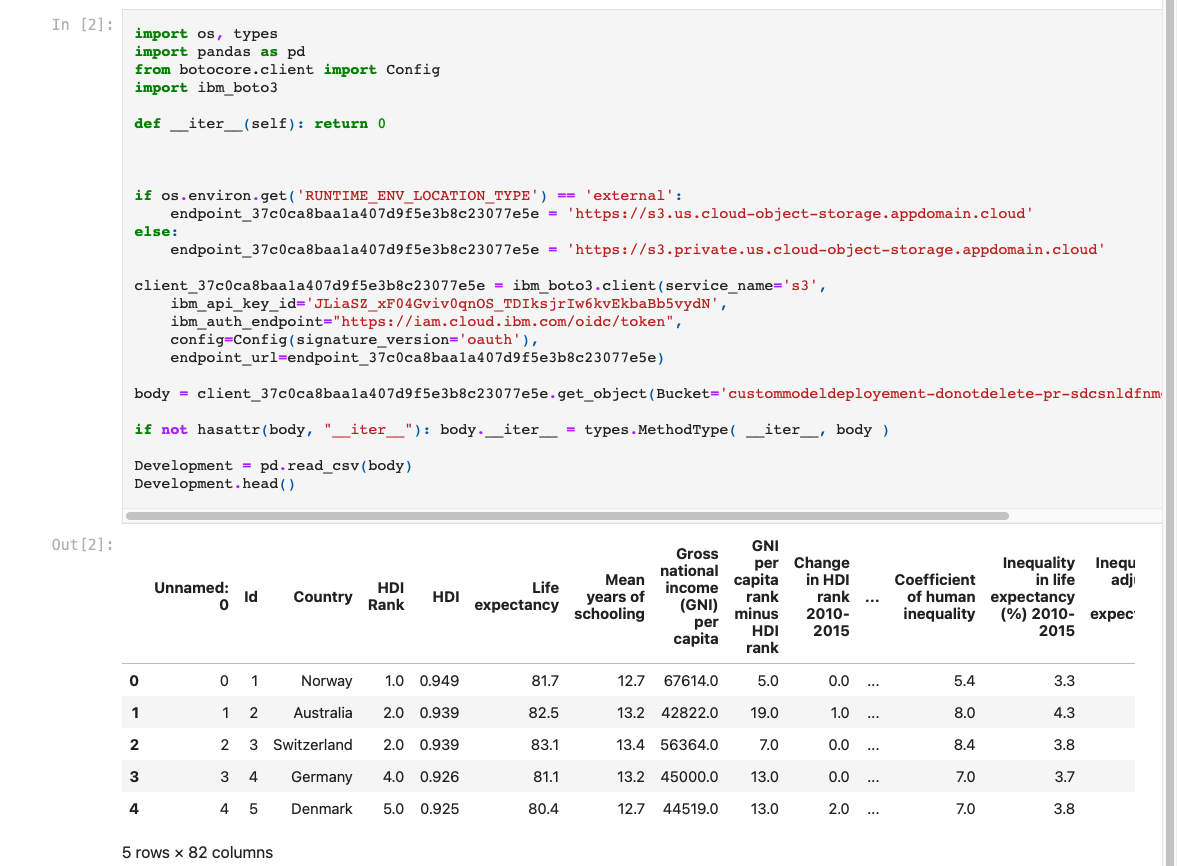
\includegraphics[width=9cm]{existingSol1Jupyter.png}};
    \draw[-{Stealth[length=5mm]}, red] (-1,5) -- (2,5);
    \node[left, red, text width=2cm] at (-1,5) {Input code snippet};
    \draw[-{Stealth[length=5mm]}, red] (-1,1) -- (2,1);
    \node[left, red, text width=2.5cm] at (-1,1) {Some Output};
\end{tikzpicture}
\caption{Jupyter Notebook Format (Not Suitable)}\label{fig:es1a}
\end{figure}
However, for my project, my model needs to be pre-trained and then accessed via a GUI, so a Jupyter Notebook is not suitable.

This solution also has a scatter plot showing the HDI of various countries (Figure \ref{fig:es1b}). It includes a select few countries, which have an HDI $\geq 0.90$, which are each represented by a coloured dot. (The specific colour seems to carry no meaning)
\begin{figure}[H]
\centering
\begin{tikzpicture}
    \node[above right, inner sep=0] (image) at (0,0) {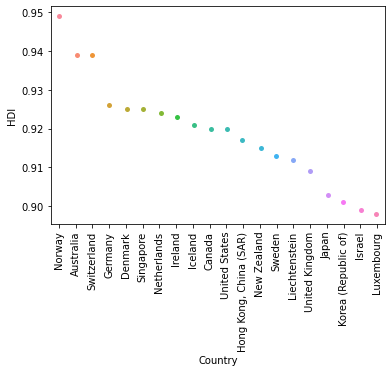
\includegraphics[width=9cm]{existingSol1Scatter.png}};
    \draw[-{Stealth[length=5mm]}, red] (7,7) -- (5,6);
    \node[right, red, text width=3cm] at (7,7) {Coloured Dots representing HDI};
    \draw[-{Stealth[length=5mm]}, red] (-1,2.75) -- (1,2.75);
    \node[left, red, text width=3cm] at (-1,2.75) {Set of High HDI Countries};
\end{tikzpicture}
\caption{HDI Scatter Plot By Country}\label{fig:es1b}
\end{figure}
I believe that a bar graph would be more appropriate, as the $x$-axis is a discrete variable (which country) and the $y$-axis is continuous (HDI). This would be good to implement in my project as the HDI in the user's area could be compared to the HDI of other countries or areas on a similar graph to this, so that if they don't fully understand the HDI scale, they can easily compare with what they know.

This solution also includes the use of a heatmap, describing the relationship between each factor they consider (Figure \ref{fig:es1c}). Brighter cells represent strong positive correlation between the factors, and darker cells represent strong negative correlation.
\begin{figure}[H]
\centering
\begin{tikzpicture}
    \node[above right, inner sep=0] (image) at (0,0) {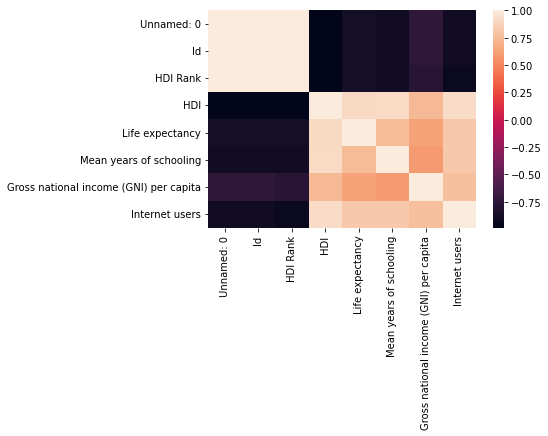
\includegraphics[width=9cm]{existingSol1Heatmap.png}};
    \draw[-{Stealth[length=5mm]}, red] (11,7.5) -- (9,6.5);
    \node[right, red, text width=3cm] at (11,7.5) {Heatmap Key};
    \draw[-{Stealth[length=5mm]}, red] (0,2.75) -- (2,3.5);
    \node[left, red, text width=2.75cm] at (0,2.75) {Some Factors Affecting HDI};
    \draw[-{Stealth[length=5mm]}, red] (9,2.75) -- (7,4);
    \node[right, red, text width=2.75cm] at (9,2.75) {Coloured Cells to Describe Relationship};
\end{tikzpicture}
\caption{HDI Factor Heatmap}\label{fig:es1c}
\end{figure}
I think it would be useful to implement this into my solution, as it would inform which changes the user needs to make to their area, in order to not only increase the general HDI, but also perhaps will improve some other things, which will even further boost the HDI.

Both of the suggested features here (Comparison of predicted HDI to other countries \& Analysis of how much each factor affects the others) will be discussed in the Stakeholder Interview (Section \ref{sec:stakeholderinterview}).

\subsubsection{julieanneco's predictingHDI \cite{existingSol2}}
This solution also has a similar heatmap feature, but here each cell has a pie chart showing the correlation coefficient (Figure \ref{fig:es2a}). The proportion of the pie that is filled carries the same meaning as the colour of the pie, with more filled in pies indicating stronger correlation. This chart also omits half of the possible combinations, as they have already been accounted for (for example, correlation between birth rate and life expectancy will be equal to the correlation between life expectancy and birth rate).
\begin{figure}[H]
\centering
\begin{tikzpicture}
    \node[above right, inner sep=0] (image) at (0,0) {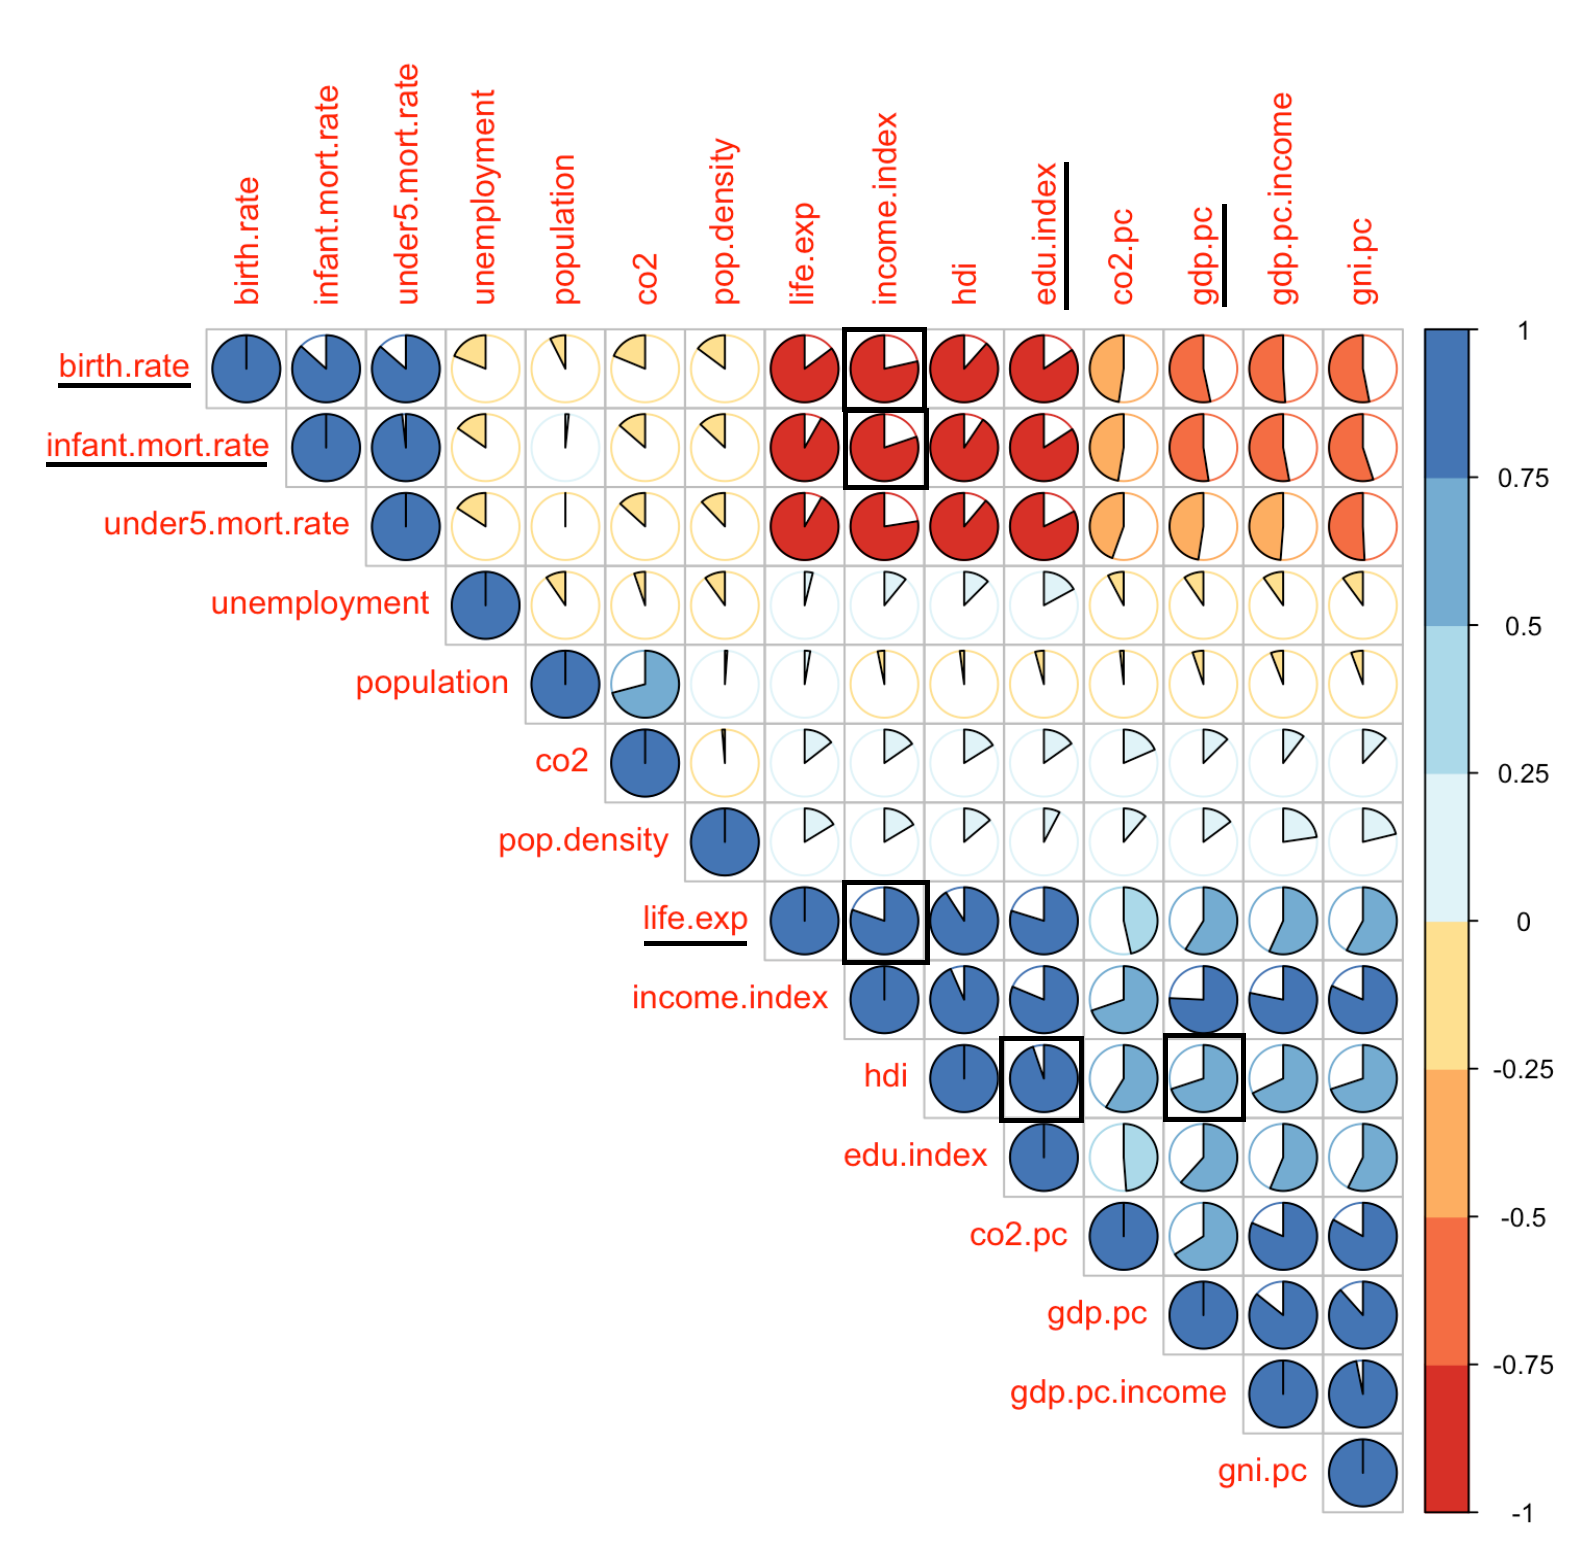
\includegraphics[width=9cm]{existingSol2Pies.png}};
    \draw[-{Stealth[length=5mm]}, red] (11,6.5) -- (9,6.5);
    \node[right, red, text width=3cm] at (11,6.5) {Heatmap Key};
    \draw[-{Stealth[length=5mm]}, red] (0.5,4) -- (2.75,4);
    \node[left, red, text width=2.75cm] at (0.5,4) {Some Factors Affecting HDI};
    \draw[-{Stealth[length=5mm]}, red] (10,4) -- (7,2.75);
    \node[right, red, text width=2.75cm] at (10,4) {Coloured Pies to Describe Relationship};
\end{tikzpicture}
\caption{HDI Factor Pie Chart Heatmap}\label{fig:es2a}
\end{figure}
While omitting half of the combinations of factors is efficient, I believe the use of pie charts in each cell only makes this chart unnecessarily more complex and harder for someone to understand. If I were to add a feature similar to this, I would only include half of it (as shown in this solution), and fill the cells with solid colour (as shown in the previous solution).

The factors that this solution take into account are more social, economic and environmental factors (Figure \ref{fig:es2b}). They have also taken into account multiple time periods (years).
\begin{figure}[H]
\centering
\begin{tikzpicture}
    \node[above right, inner sep=0] (image) at (0,0) {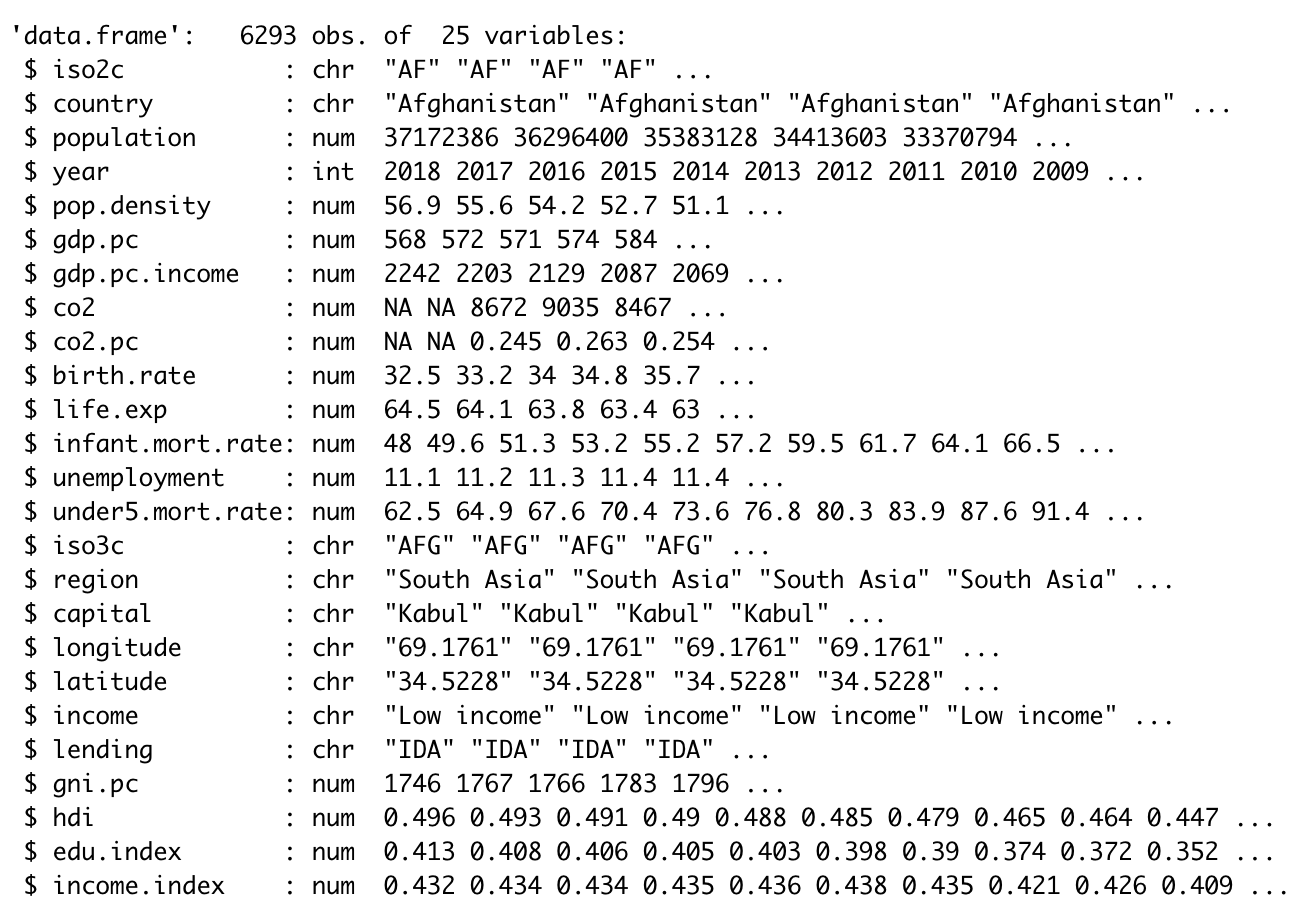
\includegraphics[width=9cm]{existingSol2Factors.png}};
    \draw[-{Stealth[length=5mm]}, red] (-2.5,4) -- (0,4);
    \node[left, red, text width=3.5cm] at (-2.5,4) {Social, Economic \& Environmental Factors};
    \draw[-{Stealth[length=5mm]}, red] (9,3.5) -- (7,5);
    \node[right, red, text width=2.75cm] at (9,3.5) {Multiple Years};
\end{tikzpicture}
\caption{Social, Economic \& Environmental Factors Across Years (Not Suitable)}\label{fig:es2b}
\end{figure}
While these are important factors in calculating HDI, this is not suitable for my project, as all of my factors are going to come from OpenStreetMaps, which only has geographical data. However, some of this geographical data will somewhat represent these factors (for example, school density will be loosely proportional to the education index (\pil{edu.index})). The use of multiple years in this solution is also not suitable for my project, as I will only be accessing the most recent version of OpenStreetMaps. Any previous versions will just be more inaccurate, as new data is constantly being added.

This solution makes use of a Random Forest Classification Algorithm to determine the HDI Class of each country at a particular time, which can either be Low, Mid or High (Figure \ref{fig:es2c}).
\begin{figure}[H]
\centering
\begin{tikzpicture}
    \node[above right, inner sep=0] (image) at (0,0) {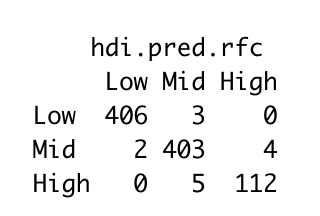
\includegraphics[width=9cm]{existingSol2Classification.png}};
    \draw[-{Stealth[length=5mm]}, red] (-2,2) -- (0.5,2);
    \node[left, red, text width=3cm] at (-2,2) {Discrete Output};
    \draw[-{Stealth[length=5mm]}, red] (9,3.5) -- (6,2);
    \node[right, red, text width=2.75cm] at (9,3.5) {Good Results};
\end{tikzpicture}
\caption{Random Forest Classification (Not Suitable)}\label{fig:es2c}
\end{figure}
While this does seem to produce good results (the HDI Class has been correctly predicted most of the time), this is not suitable for my solution, as I would like the output of my model to be continuous (the actual HDI), so I will instead be using a Multilayer Perceptron model (described later, in Section \ref{sec:mlp}).

\subsubsection{Human Development Reports' Country Insights \cite{existingSol3}}
This solution does not predict HDI, it only visualises it in different graphs. One of those is this ranking chart, which shows the HDI Rank of a particular country compared with the rest (Figure \ref{fig:es3a}).
\begin{figure}[H]
\centering
\begin{tikzpicture}
    \node[above right, inner sep=0] (image) at (0,0) {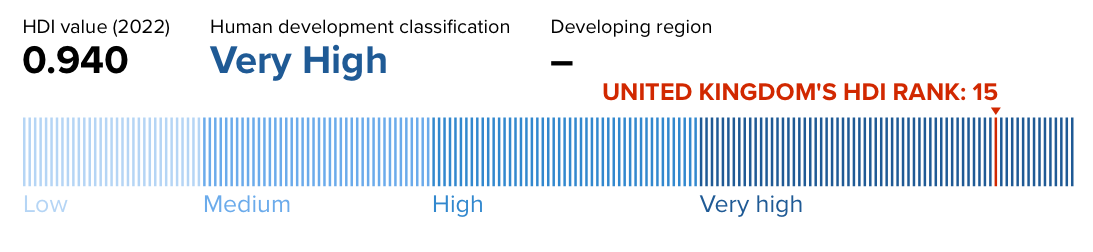
\includegraphics[width=9cm]{existingSol3Rank.png}};
    \draw[-{Stealth[length=5mm]}, red] (-2,0.75) -- (0,0.75);
    \node[left, red, text width=2.5cm] at (-2,0.75) {Bar for each Country};
    \draw[-{Stealth[length=5mm]}, red] (9,3.5) -- (7,1.5);
    \node[right, red, text width=3.25cm] at (9,3.5) {Rank for Selected Country};
\end{tikzpicture}
\caption{HDI Ranking Chart}\label{fig:es3a}
\end{figure}
You can also hover over this chart to reveal additional information for each of the other countries (Figure \ref{fig:es3b}).
\begin{figure}[H]
\centering
\begin{tikzpicture}
    \node[above right, inner sep=0] (image) at (0,0) {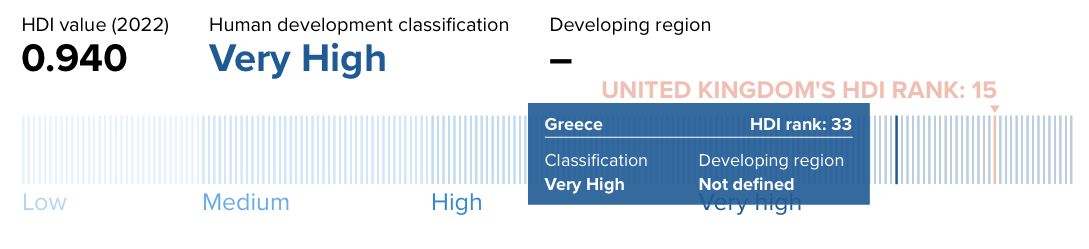
\includegraphics[width=9cm]{existingSol3Hover.png}};
    \draw[-{Stealth[length=5mm]}, red] (2,0.75) -- (4,0.75);
    \node[left, red, text width=3.25cm] at (2,0.75) {More Information};
    \draw[-{Stealth[length=5mm]}, red] (10,0.75) -- (7.5,0.75);
    \node[right, red, text width=3.25cm] at (10,0.75) {Hovered Over Country};
\end{tikzpicture}
\caption{Hovering Over HDI Ranking Chart}\label{fig:es3b}
\end{figure}
I could implement a similar chart to this, except instead of a selected country, it would be whatever region the user is predicting the HDI of, so that they can compare it to the HDI of different countries.

This solution also contains other charts, such as this waterfall chart showing HDI of a particular country over time (Figure \ref{fig:es3c}), however I believe none of these are suitable for my project, as I will only be dealing with present-day data.
\begin{figure}[H]
\centering
\begin{tikzpicture}
    \node[above right, inner sep=0] (image) at (0,0) {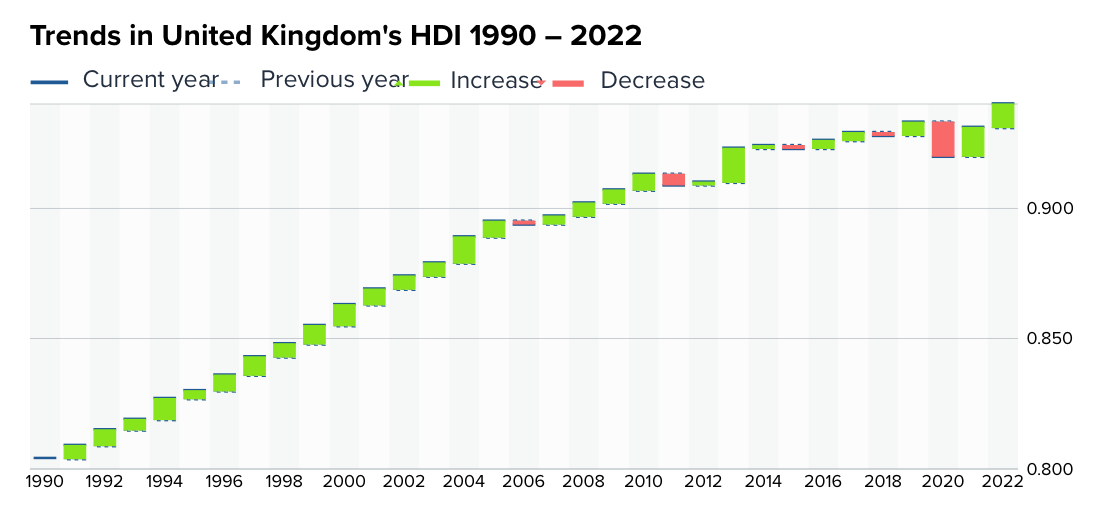
\includegraphics[width=9cm]{existingSol3Waterfall.png}};
    \draw[-{Stealth[length=5mm]}, red] (8,0.75) -- (5,2);
    \node[right, red, text width=3.25cm] at (8,0.75) {Change in HDI Over Time};
\end{tikzpicture}
\caption{HDI Over Time Waterfall Chart (Not Suitable)}\label{fig:es3c}
\end{figure}

\subsection{Stakeholder Interview \& Feedback}\label{sec:stakeholderinterview}
For this interview, coloured quotes will represent each stakeholder, as shown in the Stakeholders Table (Table \ref{table:stakeholders}).

\subsubsection{Question 1}
1. \textit{``Are you familiar with the HDI scale for development?''}
\begin{flushright}
\textit{\textcolor{Sepia}{``Yes''}} \\
\textit{\textcolor{Blue}{``Yes''}} \\
\textit{\textcolor{olive}{``Yes''}} \\
\textit{\textcolor{OliveGreen}{``Yes''}}
\end{flushright}
For each of the following questions, each stakeholder was given the options in a random order, and was made aware that they don't need to rank all of them.

\subsubsection{Question 2}
2. \textit{``Rank the following end-features by how important you believe they are.''}
\begin{center}
\begin{tabular}{c}
    Analysis of how much each factor affects the others \\
    Comparison of predicted HDI to other countries \\
    Ranking of suggested changes to increase development
\end{tabular}
\end{center}
\begin{flushright}
\textit{\textcolor{Sepia}{``1. Ranking of suggested changes to increase development \\ 2. Analysis of how much each factor affects the others \\ 3. Comparison of predicted HDI to other countries''}} \\
\textit{\textcolor{Blue}{``1. Analysis of how much each factor affects the others \\ 2. Comparison of predicted HDI to other countries \\ 3. Ranking of suggested changes to increase development''}} \\
\textit{\textcolor{olive}{``1. Ranking of suggested changes to increase development \\ 2. Analysis of how much each factor affects the others \\ 3. Comparison of predicted HDI to other countries''}} \\
\textit{\textcolor{OliveGreen}{``1. Ranking of suggested changes to increase development \\ 2. Analysis of how much each factor affects the others \\ 3. Comparison of predicted HDI to other countries''}}
\end{flushright}
To decide which feature is the most wanted from this data, each option will be awarded $\left(4-p\right)$ points for each ranking, where $p$ is the place that it was ranked (for example, if it was ranked in first place, it would gain 3 points).
\pgfplotstableread{
Label umanga joel victor kiefer topper
{Ranking Suggested Changes} 3 1 3 3 0.001
{Analysis of Factors affecting each other} 2 3 2 2 0.001
{Comparison to Other Countries} 1 2 1 1 0.001
}\endfeaturedata
\begin{figure}[H]
\centering
\begin{tikzpicture}
\begin{axis}[
    ybar stacked,
    ymin=0,
    ymax=12,
    ylabel=Points,
    xtick=data,
    xticklabels from table={\endfeaturedata}{Label},
    xticklabel style={text width=2cm,align=center},
]
\addplot [fill=red!60] table [y=umanga, meta=Label, x expr=\coordindex] {\endfeaturedata};
\addplot [fill=blue!60] table [y=joel, meta=Label, x expr=\coordindex] {\endfeaturedata};
\addplot [fill=yellow!80] table [y=victor, meta=Label, x expr=\coordindex] {\endfeaturedata};
\addplot [fill=green!80] table [y=kiefer, meta=Label, x expr=\coordindex] {\endfeaturedata};
\addplot [nodes near coords,point meta=y,nodes near coords style={anchor=south}] table [y=topper, meta=Label, x expr=\coordindex] {\endfeaturedata};
\end{axis}
\end{tikzpicture}
\caption{Score for each end-feature}
\end{figure}
Both the Ranking of suggested changes to increase development and the Analysis of how much each factor affects the others seem to be popular.

\subsubsection{Notation Explanation}
The following 2 questions are about various geographical factors which may have an impact on HDI.

As many of the following factors have a similar format, I will use the notation $D\left(x\right)$ to represent ``$x$ Density'', for some object $x$ (the number of $x$ per unit area), and $A\left(x,y\right)$ to represent ``Average Distance from $x$ to nearest $y$'', for some objects $x$, $y$ (Note that $A\left(x,y\right)$ might not be the same as $A\left(y,x\right)$). The functions $A$ and $D$ will be implemented later, in Section \ref{sec:dataCollection}.

There are many factors to consider which are directly linked to HDI, such as $D\left(\text{School}\right)$ or $D\left(\text{Hospital}\right)$, which I believe are essential factors to be considered. Therefore, I have decided to only ask about more ridiculous factors, such as $D\left(\text{Bench}\right)$ or $D\left(\text{Post Box}\right)$ which will have less of an effect on HDI. I have also included $D\left(\text{School}\right)$ as a test to ensure that the stakeholders fully understand the meaning of HDI (it should always rank highly).

\subsubsection{Question 3}
3. \textit{``Rank the following density factors affecting development in a particular area by how much you would like them to be implemented.''}
\begin{center}
\begin{tabular}{c c c c}
    $D\left(\text{Bench}\right)$ & $D\left(\text{Fast-Food Place}\right)$ & $D\left(\text{Lake}\right)$ & $D\left(\text{Place of Worship}\right)$ \\ 
    $D\left(\text{Pond}\right)$ & $D\left(\text{Post Box}\right)$ & $D\left(\text{Restaurant}\right)$ & $D\left(\text{Rock}\right)$ \\
    $D\left(\text{School}\right)$ & $D\left(\text{Toilet}\right)$ & $D\left(\text{Tree}\right)$ & $D\left(\text{Vending Machine}\right)$ \\
\end{tabular}
\end{center}
\begin{flushright}
\textit{\textcolor{Sepia}{``1. $D\left(\text{Toilet}\right)$, 2. $D\left(\text{School}\right)$, 3. $D\left(\text{Place of Worship}\right)$, 4. $D\left(\text{Restaurant}\right)$.''}} \\
\textit{\textcolor{Blue}{``1. $D\left(\text{School}\right)$, 2. $D\left(\text{Toilet}\right)$, 3. $D\left(\text{Restaurant}\right)$, 4. $D\left(\text{Vending Machine}\right)$, 5. $D\left(\text{Bench}\right)$, 6. $D\left(\text{Post Box}\right)$, 7. $D\left(\text{Place of Worship}\right)$, 8. $D\left(\text{Fast-Food Place}\right)$, 9. $D\left(\text{Pond}\right)$, 10. $D\left(\text{Lake}\right)$, 11. $D\left(\text{Rock}\right)$, 12. $D\left(\text{Tree}\right)$.''}} \\
\textit{\textcolor{olive}{``1. $D\left(\text{School}\right)$, 2. $D\left(\text{Restaurant}\right)$, 3. $D\left(\text{Post Box}\right)$, 4. $D\left(\text{Tree}\right)$, 5. $D\left(\text{Place of Worship}\right)$, 6. $D\left(\text{Vending Machine}\right)$, 7. $D\left(\text{Toilet}\right)$, 8. $D\left(\text{Fast-Food Place}\right)$.''}} \\
\textit{\textcolor{OliveGreen}{``1. $D\left(\text{School}\right)$, 2. $D\left(\text{Bench}\right)$, 3. $D\left(\text{Post Box}\right)$, 4. $D\left(\text{Toilet}\right)$, 5. $D\left(\text{Vending Machine}\right)$, 6. $D\left(\text{Fast-Food Place}\right)$, 8. $D\left(\text{Restaurant}\right)$, 9. $D\left(\text{Place of Worship}\right)$, 10. $D\left(\text{Tree}\right)$''}}
\textcolor{gray}{(the abscense of an option at number 7 is not a mistake, he did not seem to put anything there.)}
\end{flushright}
These rankings will be scored similarly, with each option being awarded $\left(13-p\right)$ points, where $p$ is the place that it was ranked, as there are now 12 options instead of 3. If the option was not ranked, then it won't be awarded any points. The points here are not comparable with the points from the previous question, as a different system is being used.
\pgfplotstableread{
Label umanga joel victor kiefer topper
{$D\left(\text{School}\right)$} 11 12 12 12 0.001
{$D\left(\text{Toilet}\right)$} 12 11 6 9 0.001
{$D\left(\text{Restaurant}\right)$} 9 10 11 5 0.001
{$D\left(\text{Place of Worship}\right)$} 10 6 8 4 0.001
{$D\left(\text{Post Box}\right)$} 0 7 10 10 0.001
{$D\left(\text{Vending Machine}\right)$} 0 9 7 8 0.001
{$D\left(\text{Bench}\right)$} 0 8 0 11 0.001
{$D\left(\text{Fast-Food Place}\right)$} 0 5 5 7 0.001
{$D\left(\text{Tree}\right)$} 0 1 9 3 0.001
{$D\left(\text{Pond}\right)$} 0 4 0 0 0.001
{$D\left(\text{Lake}\right)$} 0 3 0 0 0.001
{$D\left(\text{Rock}\right)$} 0 2 0 0 0.001
}\dfactordata
\begin{figure}[H]
\centering
\begin{tikzpicture}
\begin{axis}[
    width=0.75\textwidth,
    height=0.4\textwidth,
    ybar stacked,
    ymin=0,
    ymax=55,
    ylabel=Points,
    xtick=data,
    xticklabels from table={\dfactordata}{Label},
    xticklabel style={rotate=90, text width=4cm, align=right},
]
\addplot [fill=red!60] table [y=umanga, meta=Label, x expr=\coordindex] {\dfactordata};
\addplot [fill=blue!60] table [y=joel, meta=Label, x expr=\coordindex] {\dfactordata};
\addplot [fill=yellow!80] table [y=victor, meta=Label, x expr=\coordindex] {\dfactordata};
\addplot [fill=green!80] table [y=kiefer, meta=Label, x expr=\coordindex] {\dfactordata};
\addplot [nodes near coords,point meta=y,nodes near coords style={anchor=south}] table [y=topper, meta=Label, x expr=\coordindex] {\dfactordata};
\end{axis}
\end{tikzpicture}
\caption{Score for each density factor}
\end{figure}
As Expected, the most popular answer was $D\left(\text{School}\right)$. Among the other answers, $D\left(\text{Toilet}\right)$, $D\left(\text{Restaurant}\right)$, $D\left(\text{Place of Worship}\right)$, $D\left(\text{Post Box}\right)$ and $D\left(\text{Vending Machine}\right)$ all proved to be very popular, with a score $\geq 20$.

\subsubsection{Question 4}
4. \textit{``Rank the following distance factors affecting development in a particular area by how much you would like them to be implemented.''}
\begin{center}
\begin{tabular}{c c c}
    $A\left(\text{Bank},\text{Slot Machine}\right)$ & $A\left(\text{Bench},\text{Tree}\right)$ & $A\left(\text{Fast-Food Place},\text{Toilet}\right)$ \\
    $A\left(\text{House},\text{Fast-Food Place}\right)$ & $A\left(\text{House},\text{Place of Worship}\right)$ & $A\left(\text{House},\text{School}\right)$ \\
    \multicolumn{3}{c}{$A\left(\text{House},\text{Tree}\right)$}
\end{tabular}
\end{center}
\begin{flushright}
\textit{\textcolor{Sepia}{``1. $A\left(\text{House},\text{School}\right)$, 2. $A\left(\text{House},\text{Place of Worship}\right)$, 3. $A\left(\text{Fast-Food Place},\text{Toilet}\right)$.''}} \\
\textit{\textcolor{Blue}{``1. $A\left(\text{House},\text{School}\right)$, 2. $A\left(\text{Bank},\text{Slot Machine}\right)$, 3. $A\left(\text{Fast-Food Place},\text{Toilet}\right)$, 4. $A\left(\text{House},\text{Place of Worship}\right)$, 5. $A\left(\text{House},\text{Fast-Food Place}\right)$, 6. $A\left(\text{Bench},\text{Tree}\right)$, 7. $A\left(\text{House},\text{Tree}\right)$''}} \\
\textit{\textcolor{olive}{``1. $A\left(\text{Bank},\text{Slot Machine}\right)$, 2. $A\left(\text{House},\text{School}\right)$, 3. $A\left(\text{Bench},\text{Tree}\right)$, 4. $A\left(\text{House},\text{Tree}\right)$, 5. $A\left(\text{House},\text{Place of Worship}\right)$, 6. $A\left(\text{House},\text{Fast-Food Place}\right)$, 7. $A\left(\text{Fast-Food Place},\text{Toilet}\right)$''}} \\
\textit{\textcolor{OliveGreen}{``1. $A\left(\text{House},\text{School}\right)$, 2. $A\left(\text{House},\text{Tree}\right)$, 3. $A\left(\text{House},\text{Fast-Food Place}\right)$, 4. $A\left(\text{Bench},\text{Tree}\right)$, 5. $A\left(\text{House},\text{Place of Worship}\right)$, 6. $A\left(\text{Fast-Food Place},\text{Toilet}\right)$, 7. $A\left(\text{Bank},\text{Slot Machine}\right)$''}}
\end{flushright}
The scoring again will work the same as the previous 2 questions, except each option will be awarded $\left(8-p\right)$ points, where $p$ is the place that it was ranked, as there are now 7 options instead of 3 or 12.
\pgfplotstableread{
Label umanga joel victor kiefer topper
{$A\left(\text{House},\text{School}\right)$} 7 7 6 7 0.001
{$A\left(\text{House},\text{Place of Worship}\right)$} 6 4 3 3 0.001
{$A\left(\text{Bank},\text{Slot Machine}\right)$} 0 6 7 1 0.001
{$A\left(\text{Fast-Food Place},\text{Toilet}\right)$} 5 5 1 2 0.001
{$A\left(\text{Bench},\text{Tree}\right)$} 0 2 5 4 0.001
{$A\left(\text{House},\text{Tree}\right)$} 0 1 4 6 0.001
{$A\left(\text{House},\text{Fast-Food Place}\right)$} 0 3 2 5 0.001
}\afactordata
\begin{figure}[H]
\centering
\begin{tikzpicture}
\begin{axis}[
    width=0.6\textwidth,
    height=0.4\textwidth,
    ybar stacked,
    ymin=0,
    ymax=32,
    ylabel=Points,
    xtick=data,
    xticklabels from table={\afactordata}{Label},
    xticklabel style={rotate=90, text width=5.1cm, align=right},
]
\addplot [fill=red!60] table [y=umanga, meta=Label, x expr=\coordindex] {\afactordata};
\addplot [fill=blue!60] table [y=joel, meta=Label, x expr=\coordindex] {\afactordata};
\addplot [fill=yellow!80] table [y=victor, meta=Label, x expr=\coordindex] {\afactordata};
\addplot [fill=green!80] table [y=kiefer, meta=Label, x expr=\coordindex] {\afactordata};
\addplot [nodes near coords,point meta=y,nodes near coords style={anchor=south}] table [y=topper, meta=Label, x expr=\coordindex] {\afactordata};
\end{axis}
\end{tikzpicture}
\caption{Score for each distance factor}
\end{figure}
Again, the serious factor $A\left(\text{House},\text{School}\right)$ was the most popular by far, and will be included among others such as $A\left(\text{House},\text{Shop}\right)$ or $A\left(\text{House},\text{Pharmacy}\right)$. Among the other answers, $A\left(\text{House},\text{Place of Worship}\right)$, $A\left(\text{Bank},\text{Slot Machine}\right)$ and $A\left(\text{Fast-Food Place},\text{Toilet}\right)$ proved to be very popular, with a score $\geq 12$

I may ask further questions to my stakeholders as required, when I am developing my coded solution.

\section{Essential Features}
\begin{center}
\begin{longtable}{ | m{4cm} | m{11cm}| } 
    \hline
    \textbf{Feature} & \textbf{Explanation} \\ 
    \hline
    Area Selection & The user must be able to select the area to predict the HDI of. They should be able to do this by either drawing on a map, or entering the data manually. \\
    \hline
    Multilayer Perceptron & The HDI must be predicted based on a range of scalar factors, which the user has just inputted. \\
    \hline
    Ranking of Suggested Changes to increase Development & This will allow for users to make informed decisions on what needs to be done to increase the development of their area. This feature proved popular in the Stakeholder Interview. \\
    \hline
    Analysis of how much each factor affects the others & Users can determine which factors may affect others, which will further increase the development. This feature was in many of the existing solutions and was also proved popular in the Stakeholder Interview. \\
    \hline
\caption{Essential Features}
\end{longtable}
\end{center}
All of the above (except for the Multilayer Perceptron) will be implemented and accessed using a GUI.

\section{Limitations}\label{sec:limitations}
\begin{itemize}
    \item \textbf{Only 1 Time Period} -- As I am using OpenStreetMaps, I will only be able to access the data as it is now, so I won't be able to train the model on previous year's HDI. Older versions of OpenStreetMaps are only more inaccurate, so the training data will just be dirty and the final product will have a smaller chance of working.
    \item \textbf{Only Geographical Factors} -- Factors such as life expectancy will not be accounted for, as I would like all the data to come from the same place (OpenStreetMaps), such that the user can circle an area on a map and the HDI will be estimated from that.
    \begin{figure}[H]
        \centering
        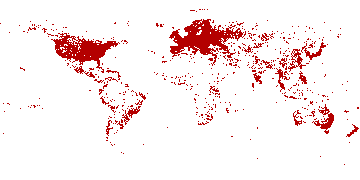
\includegraphics[width=9cm]{limitationShelter.png}
        \caption{Map of all shelters from OpenStreetMaps}\label{fig:skewMap}
    \end{figure}
    \item \textbf{Skew Towards More Developed Countries} -- OpenStreetMaps is not perfect. There will be a skew towards more developed countries because in those places, there are more people with computers who know about OpenStreetMaps, and are contributing to it. The map in Figure \ref{fig:skewMap} shows this, as it suggests that there are many more shelters in Europe than in Africa, however in reality it is likely to be the other way around.
    \item \textbf{Potential Lack of Training Data} -- HDI is only officially calculated for countries or sub-national regions (for example, in the United States, the sub-national regions are the 50 states). Therefore, I only have $\sim 2000$ pieces of data to train on (which is equal to the total number of sub-national regions), which may not be enough to get accurate results.
\end{itemize}

\section{Requirements}
\subsection{Hardware Requirements}
\begin{itemize}
    \item \textbf{Standard Input Devices (Keyboard \& Mouse)} -- I need to be able to write code and the user needs to be able to enter their details.
    \item \textbf{Monitor} -- The user and I need to be able to see the output of the program.
    \item \textbf{Main Memory} -- The program will be loaded into here when booted up.
    \item \textbf{Secondary Storage} -- The pre-trained model must be stored in secondary storage so that it can be called upon at any time.
    \item (For me only) \textbf{Graphical Processing Unit} -- While no complex graphics need to be processed, a GPU would decrease the time taken for the model to be trained, as it would involve lots of the same type of calculation (matrix multiplication) to be carried out simultaneously.
\end{itemize}
I will be using a Mac Mini, M4 to develop this app.

\subsection{Software Requirements}
\begin{itemize}
    \item (For me only) \textbf{IDE (Visual Studio Code)} -- I will write the code for this project (and the documentation) in this IDE, as it provides many useful features such as syntax highlighting, automatic bracket completion and version control (git integration).
    \item (For me only) \textbf{Python 3.10} -- The programming language I intend to write in.
    \item (For me only) \textbf{Python Libraries} Including but not limited to:
    \begin{itemize}
        \item \textbf{Gradio} -- A GUI Library, that will initialise a GUI on a local server, so that the app can be accessed from a web browser.
        \item \textbf{Numpy} -- A Maths Library, which contains many useful mathematical functions and data structures, such as matrices or multidimensional arrays, as well as the operations that come with them.
        \item \textbf{Folium} -- A Mapping Library, which will allow me to create various maps within the Gradio interface, for both input and output.
    \end{itemize}
    \item \textbf{Web Browser} -- The Gradio GUI must be accessed through a web browser. I need to be able to test the code, and the user needs to be able to use it. The user will only require a web browser as I plan to deploy this app once I have finished development.
\end{itemize}
I will be using macOS Sequoia 15.1 to develop this app.

\section{Success Criteria}
\begin{center}
\csvloop{
    file=data/successcriteria.csv,
    no head,
    column count=5,
    column names={1=\scID, 2=\scCriterion, 3=\scJustification, 4=\scSuccess, 5=\scEvaluation},
    %filter ifthen={\equal{\scID}{the thing you want}\OR\equal{\scID}{\textbf{No.}}},
    before reading={
        \begin{longtable}{|m{1cm}|m{5cm}|m{8cm}|H H}
        \hline
    },
    command=\csvlinetotablerow,
    late after line=\\\hline,
    after reading={
        \caption{Success Criteria}
        \end{longtable}
    }
}
\end{center}

\chapter{Design of the \nth{1} Prototype}
\section{Structure Diagram}
\begin{figure}[H]
\centering
\begin{forest}
forked edges,
for tree={draw,align=center,edge={-latex}},where level=0{}{folder,grow'=0}
[Predicting HDI App,fill=red!60
    [Data Collection \&\\Processing (Section \ref{sec:dataCollection}),fill=orange!60
        [Overpass Turbo\\Querier (Section \ref{sec:dataCollectionFullAlgo}),fill=yellow!60]
        [$D\left(x\right)$ (Section \ref{sec:dx}),fill=yellow!60
            [Calculate Area\\of a given Region,fill=green!60]
        ]
        [$A\left(x\comma{}y\right)$ (Section \ref{sec:axy}),fill=yellow!60
            [Calculate distance\\between 2 given\\coordinates,fill=green!60]
        ]
    ]
    [Multilayer Perceptron\\(Section \ref{sec:mlp}),fill=orange!60
        [Prediction,fill=yellow!60
            [Feedforward Algorithm\\(Section \ref{sec:feedforward}),fill=green!60]
        ]
        [Training,fill=yellow!60
            [Backpropogation\\Algorithm (Section \ref{sec:backpropogation}),fill=green!60]
            [Stochastic Gradient\\Descent (Section \ref{sec:sgd}),fill=green!60]
        ]
    ]
    [User Interface (Section \ref{sec:ui}),fill=orange!60
        [Input Map\\for Selection,fill=yellow!60]
        [Predicted HDI Output\\(Section \ref{sec:predictHDIFullAlgo}),fill=yellow!60]
        [Ranking Suggested Changes\\to Improve HDI,fill=yellow!60
            [Find Optimal Place for\\New Building (Section \ref{sec:optimalPlace}),fill=green!60]
            [Quicksort Results,fill=green!60]
        ]
        [Heatmap of how much each\\factor affects the others,fill=yellow!60]
        [Comparison to\\other countries,fill=yellow!60]
    ]
]
\end{forest}
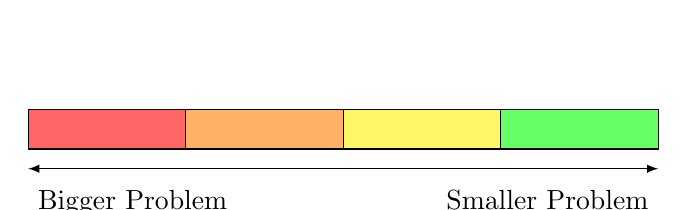
\begin{tikzpicture}
    \draw[draw=white] (-4,1) -- (4,1);
	\draw[draw=black, fill=red!60] (-4,0.5) rectangle (-2,0);
	\draw[draw=black, fill=orange!60] (-2,0.5) rectangle (0,0);
	\draw[draw=black, fill=yellow!60] (0,0.5) rectangle (2,0);
	\draw[draw=black, fill=green!60] (2,0.5) rectangle (4,0);
	\draw[draw=black, latex-latex] (-4,-0.25) -- (4,-0.25);
	\node[black, anchor=north west] at (-4,-0.4) {Bigger Problem};
	\node[black, anchor=north east] at (4,-0.4) {Smaller Problem};
\end{tikzpicture}
\caption{Structure Diagram}\label{fig:structDiagram}
\end{figure}

Figure \ref{fig:structDiagram} shows this project's structure, breaking down the larger problem of the entire app, into a series of smaller problems which are easier to consider. I will go into more detail for each of the smaller problems above (further decomposing them), in the approximate order I would be implementing them.

In this first prototype, I will be going through the algorithms involved in Data Collection \& Processing (Section \ref{sec:dataCollection}) and the Multilayer Perceptron (Section \ref{sec:mlp}), with only the most essential features in the GUI. Various data visualisations such as the Factor Heatmap or Comparisons to Other Countries will be implemented in later prototypes.

\section{Data Collection \& Processing}\label{sec:dataCollection}
\subsection{Full List of Factors to Include}\label{sec:listOfFactors}
After considering the responses from the stakeholder interview (Section \ref{sec:stakeholderinterview}), as well as research on what contributes to a higher HDI, the full list of factors I would like to consider are (in no particular order):
\begin{multicols}{2}
\begin{enumerate}
    \item $A\left(\text{House},\text{School}\right)$
    \item $A\left(\text{House},\text{Hospital}\right)$
    \item $A\left(\text{House},\text{Pharmacy}\right)$
    \item $A\left(\text{House},\text{Restaurant}\right)$
    \item $A\left(\text{School},\text{Hospital}\right)$
    \item $A\left(\text{Police},\text{Hospital}\right)$
    \item $A\left(\text{House},\text{Place of Worship}\right)$
    \item $A\left(\text{Bank},\text{Slot Machine}\right)$
    \item $A\left(\text{Fast-Food Place},\text{Toilet}\right)$
    \item $A\left(\text{House},\text{Police}\right)$
    \item $A\left(\text{University},\text{Library}\right)$
    \item $A\left(\text{House},\text{Library}\right)$
    \item $D\left(\text{School}\right)$
    \item $D\left(\text{Hospital}\right)$
    \item $D\left(\text{Pharmacy}\right)$
    \item $D\left(\text{Police}\right)$
    \item $D\left(\text{Library}\right)$
    \item $D\left(\text{Toilet}\right)$
    \item $D\left(\text{Restaurant}\right)$
    \item $D\left(\text{Place of Worship}\right)$
    \item $D\left(\text{Post Box}\right)$
    \item $D\left(\text{Vending Machine}\right)$
    \item $D\left(\text{Bench}\right)$
    \item $D\left(\text{Tree}\right)$
\end{enumerate}
\end{multicols}

Now we must figure out how to calculate $A\left(x,y\right)$, for some objects $x,y$, and $D\left(x\right)$, for some object $x$.

\subsection{Finding the Average Distance between 2 objects $x,y$, $A\left(x\comma{}y\right)$}\label{sec:axy}
\subsubsection{Finding the distance between 2 given points}
This is a difficult problem to solve, so instead decompose it and consider a simple one, finding the distance between any 2 given points on the Earth's surface (latitude longitude pairs).

First, abstract the earth into a perfectly smooth sphere (which is fairly accurate anyway as $\frac{\text{height difference between Mt. Everest and the Mariana Trench}}{\text{Earth's average radius}}=0.0031$), with centre $O$ and radius $r$, and rotated such that the plane of the equator lies on the $xy$-plane and that the point with 0 latitude and 0 longitude lies on the positive $x$-axis. I am not considering the altitude at each point on the Earth's surface, nor the slight eccentricity in the shape of the Earth.
\begin{figure}[H]
\centering
\begin{tikzpicture}[scale=4,tdplot_main_coords]
    % spherical background
    \tdplotsetrotatedcoords{-10}{90}{0}
    \draw[ball color=cyan,very thin,tdplot_rotated_coords] (0,0,0) circle (1);
    % axis
    \draw[dashed] (-1.25,0,0) -- (1.25,0,0) node[anchor=north west] {$x$};
    \draw[dashed] (0,-1.25,0) -- (0,1.25,0) node[anchor=west] {$y$};
    \draw[dashed] (0,0,-1.25) -- (0,0,1.25) node[anchor=south] {$z$};
    % equator
    \draw[dashed] (0,0,0) node[anchor=north east] {$O$} circle (1);
    % points
    \draw (0,0,0) -- (0.7071,0.7071,0) node[midway,below] {$r$};
\end{tikzpicture}
\caption{Abstracted Model of the Earth}\label{fig:abstractedEarth}
\end{figure}

The 2 points on its surface we are trying to find the distance between are $P_1$ and $P_2$, each with a latitude and longitude ($La_1$, $La_2$, $Lo_1$, $Lo_2$), given in radians.

Construct points $A$ and $B$, such that they lie directly below $P_1$ and $P_2$ respectively, and sit on the plane of the equator. By definition of latitude, $\angle P_{1}OA=La_1$ and $\angle P_{2}OB=La_2$. From right-angled trigonometry, $OA=r\cos\left(La_1\right)$ and $OB=r\cos\left(La_2\right)$
\begin{figure}[H]
\centering
\begin{tikzpicture}[scale=4,tdplot_main_coords]
    % spherical background
    \tdplotsetrotatedcoords{-10}{90}{0}
    \draw[ball color=cyan,very thin,tdplot_rotated_coords] (0,0,0) circle (1);
    % equator
    \draw[dashed] (0,0,0) coordinate (O) node[anchor=south] {$O$} circle (1);
    % points
    \draw (O) -- (0.77,0.43,0.48) coordinate (P1) node[anchor=south west] {$P_1$} node[midway,above] {$r$};
    \draw (O) -- (0.32,-0.51,0.79) coordinate (P2) node[anchor=south east] {$P_2$} node[midway,right] {$r$};
    %constructions
    \draw (O) -- (0.77,0.43,0) coordinate (A) node[anchor=north west] {$A$} -- (P1);
    \path pic["$La_1$",draw,angle radius=1.25cm] {angle=A--O--P1};
    \path pic[draw,angle radius=0.25cm] {right angle=O--A--P1};
    \draw (O) -- (0.32,-0.51,0) coordinate (B) node[anchor=north east] {$B$} -- (P2);
    \path pic["$La_2$",draw,angle radius=1cm] {angle=P2--O--B};
    \path pic[draw,angle radius=0.25cm] {right angle=O--B--P2};
    %labels
    \draw[dashed] (O) -- (-0.79,1.41,0);
    \draw[dashed] (A) -- (-0.02,1.84,0);
    \draw[<->] (-0.73,1.31,0) -- (0.04,1.74,0) node[midway,above right] {$r\cos\left(La_1\right)$};
    \draw[dashed] (O) -- (-1.37,-0.85,0);
    \draw[dashed] (B) -- (-1.05,-1.37,0);
    \draw[<->] (-1.27,-0.80,0) -- (-0.95,-1.31,0) node[midway,above left] {$r\cos\left(La_2\right)$};
\end{tikzpicture}
\caption{$P_1$ and $P_2$}
\end{figure}

Construct the line $AB$, which lies on the plane of the equator. By definition of longitude, $\angle AOB=\lvert Lo_{1}-Lo_{2}\rvert $ (the difference in longitudes). Define $a$ to be the length of the line segment $AB$, which can be found using the cosine rule.
\begin{figure}[H]
\centering
\begin{tikzpicture}[scale=4,tdplot_main_coords]
    % spherical background
    \tdplotsetrotatedcoords{-10}{90}{0}
    \draw[ball color=cyan,very thin,tdplot_rotated_coords] (0,0,0) circle (1);
    % equator
    \draw[dashed] (0,0,0) coordinate (O) node[anchor=south] {$O$} circle (1);
    % points
    \draw (O) -- (0.77,0.43,0.48) coordinate (P1) node[anchor=south west] {$P_1$} node[midway,above] {$r$};
    \draw (O) -- (0.32,-0.51,0.79) coordinate (P2) node[anchor=south east] {$P_2$} node[midway,right] {$r$};
    %constructions
    \draw (O) -- (0.77,0.43,0) coordinate (A) node[anchor=north west] {$A$} -- (P1);
    \path pic[draw,angle radius=0.25cm] {right angle=O--A--P1};
    \draw (O) -- (0.32,-0.51,0) coordinate (B) node[anchor=north east] {$B$} -- (P2);
    \path pic[draw,angle radius=0.25cm] {right angle=O--B--P2};
    \draw (A) -- (B) node[midway,below] {$a$};
    \path pic["$\lvert Lo_{1}-Lo_{2}\rvert$",draw,angle radius=0.5cm,angle eccentricity=1.2] {angle=B--O--A};
    %labels
    \draw[dashed] (O) -- (-0.79,1.41,0);
    \draw[dashed] (A) -- (-0.02,1.84,0);
    \draw[<->] (-0.73,1.31,0) -- (0.04,1.74,0) node[midway,above right] {$r\cos\left(La_1\right)$};
    \draw[dashed] (O) -- (-1.37,-0.85,0);
    \draw[dashed] (B) -- (-1.05,-1.37,0);
    \draw[<->] (-1.27,-0.80,0) -- (-0.95,-1.31,0) node[midway,above left] {$r\cos\left(La_2\right)$};
\end{tikzpicture}
\caption{Line segment $AB$}
\end{figure}
\begin{equation}\label{eq:dist2pointsa}
\begin{split}
    a=AB&=\sqrt{{OA}^2+{OB}^2-2\times OA\times OB\times \cos\left(\angle AOB\right)}\\
    &=\sqrt{{\left(r\cos\left(La_1\right)\right)}^2+{\left(r\cos\left(La_2\right)\right)}^2+2\times r\cos\left(La_1\right)\times r\cos\left(La_2\right)\times\cos\left(\lvert Lo_{1}-Lo_{2}\rvert\right)}\\
    &=\sqrt{r^{2}\cos^{2}\left(La_{1}\right)+r^{2}\cos^{2}\left(La_{2}\right)-2r^{2}\cos \left(La_{1}\right)\cos \left(La_{2}\right)\cos \left(Lo_{1}-Lo_{2}\right)}
\end{split}
\end{equation}

From right-angled trigonometry, $P_{1}A=r\sin\left(La_1\right)$ and $P_{2}B=r\sin\left(La_2\right)$. Construct the line $P_{1}P_{2}$, which will lie in the same vertical plane as $AB$ (as $P_1$ is directly above $A$ and $P_2$ is directly above $B$). If $P_1$ and $P_2$ are in the same hemisphere (north or south), then the shape $P_{1}ABP_{2}$ will be a right-angled trapezium. Define $b$ to be the length of the line segment $P_{1}P_{2}$.
\begin{figure}[H]
\centering
\begin{tikzpicture}[scale=4,tdplot_main_coords]
    % spherical background
    \tdplotsetrotatedcoords{-10}{90}{0}
    \draw[ball color=cyan,very thin,tdplot_rotated_coords] (0,0,0) circle (1);
    % equator
    \draw[dashed] (0,0,0) coordinate (O) node[anchor=south] {$O$} circle (1);
    % points
    \draw (O) -- (0.77,0.43,0.48) coordinate (P1) node[anchor=south west] {$P_1$} node[midway,above] {$r$};
    \draw (O) -- (0.32,-0.51,0.79) coordinate (P2) node[anchor=south east] {$P_2$} node[midway,right] {$r$};
    %constructions
    \draw (O) -- (0.77,0.43,0) coordinate (A) node[anchor=north west] {$A$} -- (P1) node[midway,right] {$r\sin\left(La_1\right)$};
    \path pic["$La_1$",draw,angle radius=1.25cm] {angle=A--O--P1};
    \path pic[draw,angle radius=0.25cm] {right angle=O--A--P1};
    \draw (O) -- (0.32,-0.51,0) coordinate (B) node[anchor=north east] {$B$} -- (P2) node[midway,left] {$r\sin\left(La_2\right)$};
    \path pic["$La_2$",draw,angle radius=1cm] {angle=P2--O--B};
    \path pic[draw,angle radius=0.25cm] {right angle=O--B--P2};
    \draw (A) -- (B) node[midway,below] {$a$};
    \draw (P1) -- (P2) node[midway,above] {$b$};
\end{tikzpicture}
\caption{Line segment $P_{1}P_{2}$}
\end{figure}

$b$ can be found using Pythagoras, by considering moving $AB$ up until it meets either $P_1$ or $P_2$. We don't know which one it will meet first, so the difference in heights is $\lvert P_{1}A-P_{2}B\rvert$. This will still be true even if $P_{1}ABP_{2}$ is not a trapezium (as a result of $P_1$ and $P_2$ being in opposite hemispheres), as the one in the Southern Hemisphere will have a negative height.
\begin{figure}[H]
\centering
\begin{tikzpicture}
    \draw (0,0) coordinate (B) node[anchor=north east] {$B$} -- (4,0) coordinate (A) node[anchor=north west] {$A$} node[midway,below] {$a$} -- (4,3) coordinate (P1) node[anchor=south west] {$P_1$} node[midway,right] {$r\sin\left(La_1\right)$} -- (0,5) coordinate (P2) node[anchor=south east] {$P_2$} node[midway,above] {$b$} -- cycle node[midway,left] {$r\sin\left(La_2\right)$};
    \path pic[draw,angle radius=0.25cm] {right angle=P2--B--A};
    \path pic[draw,angle radius=0.25cm] {right angle=P1--A--B};
    \draw[dashed] (P1) -- (0,3) coordinate (C) node[midway,below] {$a$};
    \path pic[draw,dashed,angle radius=0.25cm] {right angle=P2--C--P1};
    \draw[dashed] (P2) -- (-1.5,5);
    \draw[dashed] (C) -- (-1.5,3);
    \draw[<->] (-1.25,5) -- (-1.25,3) node[midway,left] {$\lvert r\sin\left(La_1\right)-r\sin\left(La_2\right)\rvert$};
\end{tikzpicture}
\caption{Finding $b$}
\end{figure}
\begin{equation}\label{eq:dist2pointsb}
\begin{split}
    b=P_{1}P_{2}&=\sqrt{{\lvert P_{1}A-P_{2}B\rvert}^2+{AB}^2}\\
    &=\sqrt{{\left(\lvert r\sin\left(La_1\right)-r\sin\left(La_2\right)\rvert\right)}^2+{a}^2}\\
    &=\sqrt{{\left(r\sin\left(La_1\right)-r\sin\left(La_2\right)\right)}^2+{a}^2}
\end{split}
\end{equation}

This is not quite what we are after, as this is the straight line distance from $P_1$ to $P_2$, but we want the distance along the surface of the Earth, which will be curved. To find this, we must find the angle $\theta$ between $P_1$ and $P_2$, which we can do by using the cosine rule in reverse.
\begin{figure}[H]
\centering
\begin{tikzpicture}[scale=4,tdplot_main_coords]
    % spherical background
    \tdplotsetrotatedcoords{-10}{90}{0}
    \draw[ball color=cyan,very thin,tdplot_rotated_coords] (0,0,0) circle (1);
    % equator
    \draw[dashed] (0,0,0) coordinate (O) node[anchor=north] {$O$} circle (1);
    % points
    \draw (O) -- (0.77,0.43,0.48) coordinate (P1) node[anchor=south west] {$P_1$} node[midway,below] {$r$};
    \draw (O) -- (0.32,-0.51,0.79) coordinate (P2) node[anchor=south east] {$P_2$} node[midway,below left] {$r$};
    %constructions
    \draw[dashed] (O) -- (0.77,0.43,0) coordinate (A) node[anchor=north west] {$A$} -- (P1);
    \path pic[draw,dashed,angle radius=0.25cm] {right angle=O--A--P1};
    \draw[dashed] (O) -- (0.32,-0.51,0) coordinate (B) node[anchor=north east] {$B$} -- (P2);
    \path pic[draw,dashed,angle radius=0.25cm] {right angle=O--B--P2};
    \draw[dashed] (A) -- (B);
    \draw (P1) -- (P2) node[midway,above] {$b$};
    \path pic["$\theta$",draw,angle radius=0.6cm] {angle=P1--O--P2};
\end{tikzpicture}
\caption{Angle $\theta$ between $P_1$ and $P_2$}
\end{figure}
\begin{equation}\label{eq:dist2pointstheta}
\begin{split}
    \theta=\angle P_{1}OP_{2}&=\arccos\left(\frac{{\left(OP_1\right)}^2+{\left(OP_2\right)}^2-{\left(P_{1}P_{2}\right)}^2}{2\times OP_1\times OP_2}\right)\\
    &=\arccos\left(\frac{{r}^2+{r}^2-{b}^2}{2\times r\times r}\right)\\
    &=\arccos\left(\frac{2{r}^2-{b}^2}{2{r}^2}\right)\\
    &=\arccos\left(1-\frac{{b}^2}{2{r}^2}\right)
\end{split}
\end{equation}

The arclength between 2 points on a circle (in this case, the great circle on the surface of the Earth containing $P_1$ and $P_2$) separated by an angle of $\theta$ is given by $\text{arclength}=r\theta$.
\begin{figure}[H]
\centering
\begin{tikzpicture}[scale=4,tdplot_main_coords]
    % spherical background
    \tdplotsetrotatedcoords{-10}{90}{0}
    \draw[ball color=cyan,very thin,tdplot_rotated_coords] (0,0,0) circle (1);
    % equator
    \draw[dashed] (0,0,0) coordinate (O) node[anchor=north] {$O$} circle (1);
    % points
    \draw (O) -- (0.77,0.43,0.48) coordinate (P1) node[anchor=south west] {$P_1$} node[midway,below] {$r$};
    \draw (O) -- (0.32,-0.51,0.79) coordinate (P2) node[anchor=south east] {$P_2$} node[midway,below left] {$r$};
    %constructions
    \draw[dashed] (O) -- (0.77,0.43,0) coordinate (A) node[anchor=north west] {$A$} -- (P1);
    \path pic[draw,dashed,angle radius=0.25cm] {right angle=O--A--P1};
    \draw[dashed] (O) -- (0.32,-0.51,0) coordinate (B) node[anchor=north east] {$B$} -- (P2);
    \path pic[draw,dashed,angle radius=0.25cm] {right angle=O--B--P2};
    \draw[dashed] (A) -- (B);
    \draw[dashed] (P1) -- (P2) node[midway,below] {$b$};
    \path pic["$\theta$",draw,angle radius=0.6cm] {angle=P1--O--P2};
    \tdplotdefinepoints(0,0,0)(0.77,0.43,0.48)(0.32,-0.51,0.79)
    \tdplotdrawpolytopearc[]{1}{}{}
\end{tikzpicture}
\caption{Arc between $P_1$ and $P_2$}
\end{figure}
Substituting $\theta$ for equation \ref{eq:dist2pointstheta} gives
\begin{equation}
    \text{arclength}=r\arccos \left(1-\frac{b^{2}}{2r^{2}}\right)
\end{equation}

Substituting $b$ for equation \ref{eq:dist2pointsb} gives
\begin{equation}
\begin{split}
    \text{arclength}&=r\arccos \left(1-\frac{{\left(r\sin\left(La_{1}\right)-r\sin\left(La_{2}\right)\right)}^{2}+a^{2}}{2r^{2}}\right)\\
    &=r\arccos \left(1-\frac{r^{2}\sin^{2}\left(La_{1}\right)-2r^{2}\sin\left(La_{1}\right)\sin\left(La_{2}\right)+r^{2}\sin^{2}\left(La_{2}\right)+a^{2}}{2r^{2}}\right)
\end{split}
\end{equation}

Substituting $a$ for equation \ref{eq:dist2pointsa} gives

\begin{equation}
\begin{split}
    \text{arclength}&=r\arccos \left(1-\frac{r^{2}\left(\splitdfrac{\sin^{2}\left(La_{1}\right)-2\sin\left(La_{1}\right)\sin\left(La_{2}\right)+\sin^{2}\left(La_{2}\right)+\cos^{2}\left(La_{1}\right)}{+\cos^{2}\left(La_{2}\right)-2\cos \left(La_{1}\right)\cos \left(La_{2}\right)\cos \left(Lo_{1}-Lo_{2}\right)}\right)}{2r^{2}}\right)\\
    &=r\arccos \left(1-\frac{\splitdfrac{\sin^{2}\left(La_{1}\right)+\cos^{2}\left(La_{1}\right)+\sin^{2}\left(La_{2}\right)+\cos^{2}\left(La_{2}\right)}{-2\sin\left(La_{1}\right)\sin\left(La_{2}\right)-2\cos \left(La_{1}\right)\cos \left(La_{2}\right)\cos \left(Lo_{1}-Lo_{2}\right)}}{2}\right)\\
    &=r\arccos \left(1-\frac{2-2\sin\left(La_{1}\right)\sin\left(La_{2}\right)-2\cos \left(La_{1}\right)\cos \left(La_{2}\right)\cos \left(Lo_{1}-Lo_{2}\right)}{2}\right)\\
    &=r\arccos \left(1-\left(1-\sin\left(La_{1}\right)\sin\left(La_{2}\right)-\cos \left(La_{1}\right)\cos \left(La_{2}\right)\cos \left(Lo_{1}-Lo_{2}\right)\right)\right)\\
    &=r\arccos \left(\sin\left(La_{1}\right)\sin\left(La_{2}\right)+\cos \left(La_{1}\right)\cos \left(La_{2}\right)\cos \left(Lo_{1}-Lo_{2}\right)\right)
\end{split}
\end{equation}

Therefore, the distance in \unit{km} between 2 latitude and longitude coordinates along the surface of the Earth is given by:
\begin{equation}\label{eq:dist2points}
    \text{distance}=r\arccos \left(\sin\left(La_{1}\right)\sin\left(La_{2}\right)+\cos \left(La_{1}\right)\cos \left(La_{2}\right)\cos \left(Lo_{1}-Lo_{2}\right)\right)
\end{equation}
where $r$ is the radius of the Earth in \unit{km} and $La_1$, $La_2$, $Lo_1$ and $Lo_2$ are the 2 points' latitudes and longitudes in radians.

However, the latitude and longitude coordinates returned by OpenStreetMaps are not measured in radians, but instead measured in degrees, so we must use the conversion factor $\left(\text{angle in radians}\right)=\frac{\pi}{180}\times\left(\text{angle in degrees}\right)$ on each one before they are passed into the formula.

\subsubsection{Finding the Average Distance between 2 objects $x,y$, $A\left(x\comma{}y\right)$}
Now that we have the means to find the distance between any 2 points along the Earth's surface, we can consider the average distance between 2 particular types of object. Recall that $A\left(x,y\right)$ is specifically defined as ``Average Distance from $x$ to nearest $y$'' (for example, $x$ might be House, and $y$ might be School), so the input for this function will be 2 sets of lists of latitude and longitude coordinates, corresponding to all the $x$-objects and $y$-objects in a particular area.

As there are likely to be hundreds of thousands of each object (depending on how large of an area the user selects), it will take too long to calculate the average distance over all of these data points. This is important to consider, as this function will be run thousands of times, both in preparing the data (for me only) and when users are using the app.

Therefore, instead of considering every single data point, randomly sample an arbitrary 500 of the $x$-objects (and if there are less than 500, consider all of them), and then find out which of the $y$-objects is closest to each of them. We must consider every $y$-object for each considered $x$-object as we don't know which one will be closest to that $x$. Considering all the $y$-objects should be fine, as for all the factors in the form $A\left(x,y\right)$, there will be many more $x$-objects than $y$-objects (for example, there are many more houses than schools).

\begin{figure}[H]
\centering
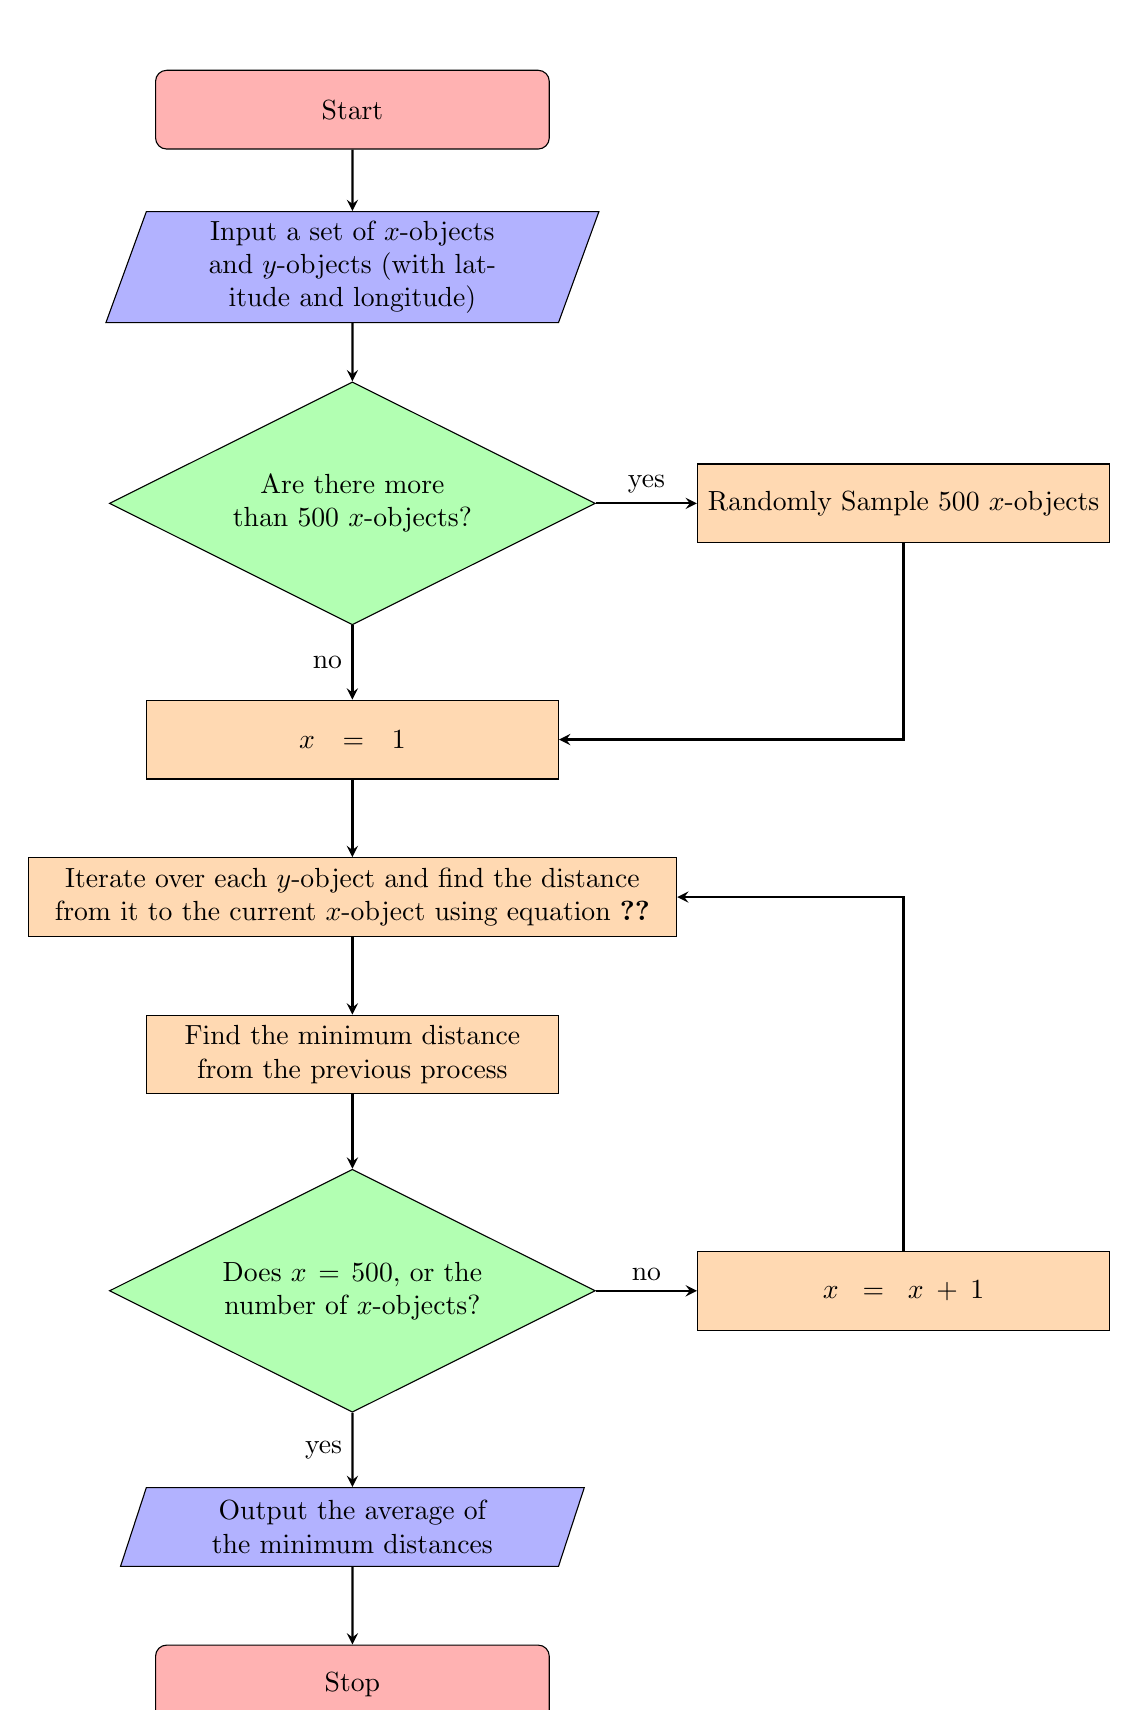
\begin{tikzpicture}[node distance=2cm]
    \node (start) [fStartStop] {Start};
    \node (incoords) [fInputOutput, below of=start] {Input a set of $x$-objects and $y$-objects (with latitude and longitude)};
    \node (decision1) [fDecision, below of=incoords, yshift=-1cm] {Are there more than 500 $x$-objects?};
    \node (randomsample) [fProcess, right of=decision1, xshift=5cm] {Randomly Sample 500 $x$-objects};
    \node (xequals1) [fProcess, below of=decision1, yshift=-1cm] {$x=1$};
    \node (getdistances) [fProcess, below of=xequals1, text width=8cm] {Iterate over each $y$-object and find the distance from it to the current $x$-object using equation \ref{eq:dist2points}};
    \node (findmin) [fProcess, below of=getdistances] {Find the minimum distance from the previous process};
    \node (decision2) [fDecision, below of=findmin, yshift=-1cm] {Does $x=500$, or the number of $x$-objects?};
    \node (incrementx) [fProcess, right of=decision2, xshift=5cm] {$x=x+1$};
    \node (output) [fInputOutput, below of=decision2, yshift=-1cm] {Output the average of the minimum distances};
    \node (stop) [fStartStop, below of=output] {Stop};
    
    \draw [fArrow] (start) -- (incoords);
    \draw [fArrow] (incoords) -- (decision1);
    \draw [fArrow] (decision1) -- node[anchor=south] {yes} (randomsample);
    \draw [fArrow] (randomsample) |- (xequals1);
    \draw [fArrow] (decision1) -- node[anchor=east] {no} (xequals1);
    \draw [fArrow] (xequals1) -- (getdistances);
    \draw [fArrow] (getdistances) -- (findmin);
    \draw [fArrow] (findmin) -- (decision2);
    \draw [fArrow] (decision2) -- node[anchor=east] {yes} (output);
    \draw [fArrow] (decision2) -- node[anchor=south] {no} (incrementx);
    \draw [fArrow] (incrementx) |- (getdistances);
    \draw [fArrow] (output) -- (stop);
\end{tikzpicture}
\caption{$A\left(x,y\right)$ Flowchart}\label{fig:aofxy}
\end{figure}
For validation, if the entered list of $x$-objects is empty (in other words, there does not exist any $x$-objects in the region), the average distance returned should be infinity.

\subsection{Finding the Density of some object $x$, $D\left(x\right)$}\label{sec:dx}
\subsubsection{Definition of $D\left(x\right)$}
The density of some object is defined as ``The number of that object per unit area''. Therefore, $D\left(x\right)$ is
\begin{equation}
    \frac{\text{Total number of }x\text{-objects in a given region}}{\text{Area of that region}}
\end{equation}
Finding the total number of $x$-objects in a region is easy. As they will come in a list, we just need to find the length of that list. However, finding the area of that region is much harder, as the only information we have about it is a list (of unknown size) of its bounding latitude and longitude coordinates.

To do this, I will be using the same abstraction for the Earth, as shown in Figure \ref{fig:abstractedEarth}.

\subsubsection{Area of a Polygon on the Surface of a Sphere}
First, assume that any polygon on the surface of a sphere (any region that the user may draw) can be cut into a series of internal spherical triangles (in fact, a spherical polygon with $n$ sides can always be broken up into $n-2$ spherical triangles).
\begin{figure}[H]
\centering
\begin{tikzpicture}[scale=4,tdplot_main_coords]
    % spherical background
    \tdplotsetrotatedcoords{-10}{90}{0}
    \draw[ball color=cyan,very thin,tdplot_rotated_coords] (0,0,0) circle (1);
    % equator
    \draw[dashed] (0,0,0) node {$O$} circle (1);
    % arcs
    \tdplotdefinepoints(0,0,0)(0.62,-0.62,0.49)(0.56,-0.27,0.78)
    \tdplotdrawpolytopearc[]{1}{}{}
    \tdplotdefinepoints(0,0,0)(0.56,-0.27,0.78)(0.76,0.48,0.44)
    \tdplotdrawpolytopearc[]{1}{}{}
    \tdplotdefinepoints(0,0,0)(0.76,0.48,0.44)(0.96,-0.1,0.27)
    \tdplotdrawpolytopearc[]{1}{}{}
    \tdplotdefinepoints(0,0,0)(0.96,-0.1,0.27)(0.89,0.37,-0.28)
    \tdplotdrawpolytopearc[]{1}{}{}
    \tdplotdefinepoints(0,0,0)(0.89,0.37,-0.28)(0.87,0.03,-0.5)
    \tdplotdrawpolytopearc[]{1}{}{}
    \tdplotdefinepoints(0,0,0)(0.87,0.03,-0.5)(0.92,-0.36,-0.16)
    \tdplotdrawpolytopearc[]{1}{}{}
    \tdplotdefinepoints(0,0,0)(0.92,-0.36,-0.16)(0.61,-0.76,-0.23)
    \tdplotdrawpolytopearc[]{1}{}{}
    \tdplotdefinepoints(0,0,0)(0.61,-0.76,-0.23)(0.62,-0.62,0.49)
    \tdplotdrawpolytopearc[]{1}{}{}
    % cuts
    \tdplotdefinepoints(0,0,0)(0.62,-0.62,0.49)(0.76,0.48,0.44)
    \tdplotdrawpolytopearc[dashed,red]{1}{}{}
    \tdplotdefinepoints(0,0,0)(0.62,-0.62,0.49)(0.96,-0.1,0.27)
    \tdplotdrawpolytopearc[dashed,red]{1}{}{}
    \tdplotdefinepoints(0,0,0)(0.96,-0.1,0.27)(0.87,0.03,-0.5)
    \tdplotdrawpolytopearc[dashed,red]{1}{}{}
    \tdplotdefinepoints(0,0,0)(0.96,-0.1,0.27)(0.92,-0.36,-0.16)
    \tdplotdrawpolytopearc[dashed,red]{1}{}{}
    \tdplotdefinepoints(0,0,0)(0.62,-0.62,0.49)(0.92,-0.36,-0.16)
    \tdplotdrawpolytopearc[dashed,red]{1}{}{}
\end{tikzpicture}
\caption{Cutting into Triangles}
\end{figure}

To find the area of the polygon, we can individually find the area of each triangle and then add them up.

To find the area of a triangle on the surface of the sphere, consider extending the sides of the triangle to make great circles around the sphere.
\begin{figure}[H]
\centering
\begin{tikzpicture}[scale=4,tdplot_main_coords]
    % spherical background
    \tdplotsetrotatedcoords{-10}{90}{0}
    \draw[ball color=cyan,very thin,tdplot_rotated_coords] (0,0,0) circle (1);
    % A = (0.72,-0.66,-0.19), B=(0.9,0.38,-0.19), C=(0.72,-0.09,0.68)
    % arcs
    \tdplotdefinepoints(0,0,0)(0.72,-0.66,-0.19)(0.9,0.38,-0.19) %AB
    \tdplotdrawpolytopearc[]{1}{}{}
    \tdplotdefinepoints(0,0,0)(0.9,0.38,-0.19)(0.72,-0.09,0.68) %BC
    \tdplotdrawpolytopearc[]{1}{}{}
    \tdplotdefinepoints(0,0,0)(0.72,-0.09,0.68)(0.72,-0.66,-0.19) %CA
    \tdplotdrawpolytopearc[]{1}{}{}
    % extensions
    %AB
    \tdplotdefinepoints(0,0,0)(0.72,-0.66,-0.19)(-0.17,-0.99,0)
    \tdplotdrawpolytopearc[]{1}{}{}
    \tdplotdefinepoints(0,0,0)(0.9,0.38,-0.19)(0.01,1,0.04)
    \tdplotdrawpolytopearc[]{1}{}{}
    \tdplotdefinepoints(0,0,0)(-0.17,-0.99,0)(0.01,1,0.04)
    \tdplotdrawpolytopearc[dashed]{1}{}{}
    %BC
    \tdplotdefinepoints(0,0,0)(0.9,0.38,-0.19)(0.5,0.49,-0.71)
    \tdplotdrawpolytopearc[]{1}{}{}
    \tdplotdefinepoints(0,0,0)(0.72,-0.09,0.68)(-0.42,-0.49,0.76)
    \tdplotdrawpolytopearc[]{1}{}{}
    \tdplotdefinepoints(0,0,0)(0.5,0.49,-0.71)(-0.42,-0.49,0.76)
    \tdplotdrawpolytopearc[dashed]{-1}{}{}
    %CA
    \tdplotdefinepoints(0,0,0)(0.72,-0.09,0.68)(-0.23,0.65,0.73)
    \tdplotdrawpolytopearc[]{1}{}{}
    \tdplotdefinepoints(0,0,0)(0.72,-0.66,-0.19)(0.17,-0.62,-0.76)
    \tdplotdrawpolytopearc[]{1}{}{}
    \tdplotdefinepoints(0,0,0)(-0.23,0.65,0.73)(0.17,-0.62,-0.76)
    \tdplotdrawpolytopearc[dashed]{1}{}{}
    % angles
    \coordinate (A) at (0.72,-0.66,-0.19);
    \coordinate (B) at (0.9,0.38,-0.19);
    \coordinate (C) at (0.72,-0.09,0.68);
    \path pic["$\alpha$",draw,angle radius=0.6cm] {angle=B--A--C};
    \path pic["$\beta$",draw,angle radius=0.6cm] {angle=C--B--A};
    \path pic["$\gamma$",draw,angle radius=0.6cm] {angle=A--C--B};
\end{tikzpicture}
\caption{Triangle Edges Extended}\label{fig:areaSphere}
\end{figure}

As you can see from Figure \ref{fig:areaSphere}, the total surface area of the sphere can be given by the sum of these 6 ``spherical lune'' shapes, with an excess of 4 of the triangles we want (at either end of the sphere, the triangle is formed by the intersection of 3 spherical lunes, and so therefore we must subtract 2 for each side to get the full area of the sphere with no excess, which is why we must subtract 4 triangles overall).
\begin{equation}\label{eq:totalAreaSphere}
    A_{\text{Sphere}}=\displaystyle\sum A_{\text{Lune}}-4A_{\text{Triangle}}
\end{equation}

The surface area of a sphere is $4\pi r^2$, and the area of a spherical lune of an angle $\theta$ can be given as a fraction of the full area of the sphere.
\begin{figure}[H]
\centering
\begin{tikzpicture}[scale=4,tdplot_main_coords]
    % spherical background
    \tdplotsetrotatedcoords{-10}{90}{0}
    \draw[ball color=cyan,very thin,tdplot_rotated_coords] (0,0,0) circle (1);
    % A = (0.72,-0.66,-0.19), B=(0.9,0.38,-0.19), C=(0.72,-0.09,0.68)
    % arcs
    \tdplotdefinepoints(0,0,0)(0.9,0.38,-0.19)(0.72,-0.09,0.68) %BC
    \tdplotdrawpolytopearc[]{1}{}{}
    \tdplotdefinepoints(0,0,0)(0.72,-0.09,0.68)(0.72,-0.66,-0.19) %CA
    \tdplotdrawpolytopearc[]{1}{}{}
    % extensions
    %BC
    \tdplotdefinepoints(0,0,0)(0.9,0.38,-0.19)(0.5,0.49,-0.71)
    \tdplotdrawpolytopearc[]{1}{}{}
    \tdplotdefinepoints(0,0,0)(0.5,0.49,-0.71)(-0.72,0.09,-0.68)
    \tdplotdrawpolytopearc[dashed]{1}{}{}
    %CA
    \tdplotdefinepoints(0,0,0)(0.72,-0.66,-0.19)(0.17,-0.62,-0.76)
    \tdplotdrawpolytopearc[]{1}{}{}
    \tdplotdefinepoints(0,0,0)(0.17,-0.62,-0.76)(-0.72,0.09,-0.68)
    \tdplotdrawpolytopearc[dashed]{1}{}{}
    % angles
    \coordinate (A) at (0.72,-0.66,-0.19);
    \coordinate (B) at (0.9,0.38,-0.19);
    \coordinate (C) at (0.72,-0.09,0.68);
    \path pic["$\theta$",draw,angle radius=0.6cm] {angle=A--C--B};
\end{tikzpicture}
\caption{Area of a Spherical Lune}
\end{figure}
\begin{equation}
\begin{split}
    A_{\text{Lune}}&=\frac{\theta}{2\pi}\times 4\pi r^2\\
    &=2\theta r^2
\end{split}
\end{equation}

The 6 lunes shown in Figure \ref{fig:areaSphere} can be broken down into 3 sets of 2 identical lunes, with angles $\alpha$, $\beta$ and $\gamma$. Therefore, from equation \ref{eq:totalAreaSphere}
\begin{equation}
\begin{split}
    A_{\text{Triangle}}&=\frac{\displaystyle\sum A_{\text{Lune}}-A_{\text{Sphere}}}{4}\\
    &=\frac{2\times\left(2\alpha r^2+2\beta r^2+2\gamma r^2\right)-4\pi r^2}{4}\\
    &=\frac{4r^2\left(\alpha+\beta+\gamma-\pi\right)}{4}\\
    &=r^2\left(\displaystyle\sum\theta-\pi\right)
\end{split}
\end{equation}
where $\displaystyle\sum\theta$ represents the sum of the angles in the spherical triangle.

As our original region (an $n$-sided spherical polygon) was split up into $n-2$ spherical triangles, we can see that the area of the region $R$ is given by
\begin{equation}
\begin{split}
    R&=\displaystyle\sum_{i=1}^{n-2} {\left(A_{\text{Triangle}}\right)}_i\\
    &=\displaystyle\sum_{i=1}^{n-2} r^2\left({\left(\displaystyle\sum\theta\right)}_i-\pi\right)\\
    &=r^2\left(\displaystyle\sum_{i=1}^{n-2}{\left(\displaystyle\sum\theta\right)}_i-\left(n-2\right)\pi\right)
\end{split}
\end{equation}
where ${\left(\displaystyle\sum\theta\right)}_i$ represents the sum of the angles in spherical triangle $i$.

As the sum of the angles in a polygon equals the sum of all the sums of angles in the triangles it was broken up into, this simplifies to
\begin{equation}\label{eq:areaRegion}
    R=r^2\left(\displaystyle\sum\theta-\left(n-2\right)\pi\right)
\end{equation}
where $\displaystyle\sum\theta$ represents the sum of the interior angles in the spherical polygon, and $n$ is the number of sides of the spherical polygon.

\subsubsection{Finding the Interior Angles}
To find the interior angles of our polygon, we could use the cosine rule in reverse, as before. However, as $\cos\theta\equiv\cos\left(360-\theta\right)$, this will essentially result in both the interior angle and exterior angle for all the vertices, with no indication of which ones which. Therefore, we must introduce some directionality, by considering vectors.

The vectors we want to consider are those in the plane tangent to the point in which we want to find the interior angle of.
\begin{figure}[H]
\centering
\begin{tikzpicture}[scale=4,tdplot_main_coords]
    % spherical background
    \tdplotsetrotatedcoords{-10}{90}{0}
    \draw[ball color=cyan,very thin,tdplot_rotated_coords] (0,0,0) circle (1);
    % equator
    \draw[dashed] (0,0,0) node {$O$} circle (1);
    % arcs
    \tdplotdefinepoints(0,0,0)(0.29,-0.51,0.81)(0.66,0.21,0.72)
    \tdplotdrawpolytopearc[]{1}{}{}
    \tdplotdefinepoints(0,0,0)(0.66,0.21,0.72)(0.9,0.38,0.2)
    \tdplotdrawpolytopearc[]{1}{}{}
    % plane
    \filldraw[draw=red,fill=red!50,fill opacity=0.5] (0.44,-0.72,1.2) -- (-0.07,0.83,1.21) -- (0.89,1.15,0.23) -- (1.39,-0.4,0.23) -- cycle;
    % vectors
    \draw[->] (0.51,-0.44,1.05) -- (0.66,0.21,0.72);
    \draw[dashed] (0.51,-0.44,1.05) -- (0.29,-0.51,0.81);
    \draw[->] (0.66,0.21,0.72) -- (1.02,0.42,0.33);
    \draw[dashed] (1.02,0.42,0.33) -- (0.9,0.38,0.2);
\end{tikzpicture}
\caption{Considering Vectors}
\end{figure}

To find these vectors, we first must convert each of the coordinates from their latitude-longitude forms into their 3D position vector forms ($xyz$ coordinates).
\begin{equation}\label{eq:convert2vectors}
    \begin{pmatrix}x\\y\\z\end{pmatrix}=\begin{pmatrix}r\cos\left(La\right)\cos\left(Lo\right)\\r\cos\left(La\right)\sin\left(Lo\right)\\r\sin\left(La\right)\end{pmatrix}
\end{equation}
where $La$ is the latitude of the point, $Lo$ is the longitude of the point, and $r$ is the radius of the Earth. As we are only using this to find angles, the radius of the Earth is actually irrelevant, and so to simplify things, we can let $r=1$.

Finding these vectors on a plane which is rotated strangely is difficult, so we can instead rotate the whole system such that this plane lies on the $xy$-plane. This can be done by rotating it about the $z$-axis anticlockwise by an angle of $-Lo$, by using the matrix
\begin{equation}\label{eq:transformCoordsStart}
    \begin{pmatrix}\cos\left(-Lo\right)&-\sin\left(-Lo\right)&0\\\sin\left(-Lo\right)&\cos\left(-Lo\right)&0\\0&0&1\end{pmatrix}
\end{equation}
followed by rotating it about the $y$-axis anticlockwise by an angle of $La-90^{\circ}$, by using the matrix
\begin{equation}
    \begin{pmatrix}\cos\left(La-90^{\circ}\right)&0&\sin\left(La-90^{\circ}\right)\\0&1&0\\-\sin\left(La-90^{\circ}\right)&0&\cos\left(La-90^{\circ}\right)\end{pmatrix}
\end{equation}
finally followed by translating it down by 1 unit (as, for now, $r=1$), by adding the vector
\begin{equation}\label{eq:transformCoordsEnd}
    \begin{pmatrix}0\\0\\-1\end{pmatrix}
\end{equation}

This will have the effect of moving the point we want to find the angle at, to $\left(0,0,0\right)$, while transforming the other points in the same way.

As the plane with the vectors we want to find is now the $xy$-plane, all we need to do to project the other points onto that plane is set their $z$-coordinates to 0.
\begin{figure}[H]
\centering
\begin{tikzpicture}[scale=4,tdplot_main_coords]
    % spherical background
    \tdplotsetrotatedcoords{-10}{90}{0}
    \draw[ball color=cyan,very thin,tdplot_rotated_coords] (0,0,2.7183) circle (1);
    \node[anchor=north east] (0,0,0) {$O$};
    % axis
    \draw[dashed] (-1.25,0,0) -- (1.25,0,0) node[anchor=north west] {$x$};
    \draw[dashed] (0,-1.25,0) -- (0,1.25,0) node[anchor=west] {$y$};
    \draw[dashed] (0,0,-2.25) -- (0,0,0.75) node[anchor=south] {$z$};
    % equator
    \draw[dashed] (0,0,-1) circle (1);
    % plane
    \filldraw[draw=red,fill=red!50,fill opacity=0.5] (1,1,0) -- (-1,1,0) -- (-1,-1,0) -- (1,-1,0) -- cycle;
    % arcs
    \tdplotdefinepoints(0,0,-1)(0.35,-0.9,-0.73)(0,0,0)
    \tdplotdrawpolytopearc[]{1}{}{}
    \tdplotdefinepoints(0,0,-1)(0,0,0)(0.51,0.62,-0.41)
    \tdplotdrawpolytopearc[]{1}{}{}
    % vectors
    \draw[->] (0.35,-0.9,0) node[left] {$A$} -- (0,0,0) node[midway,above] {$\overrightarrow{AO}$};
    \draw[dashed] (0.35,-0.9,-0.73) -- (0.35,-0.9,0);
    \draw[->] (0,0,0) -- (0.51,0.62,0) node[right] {$B$} node[midway,above] {$\overrightarrow{OB}$};
    \draw[dashed] (0.51,0.62,-0.41) -- (0.51,0.62,0);
\end{tikzpicture}
\caption{Projecting the Other Points onto the $xy$-plane}
\end{figure}

As the points will be given in a list, in the other the user has drawn them in the polygon, $\overrightarrow{AO}$ (the vector from the projection of the previous point to the current point) will be given by the coordinates of $A$ times $-1$, and $\overrightarrow{OB}$ (the vector from the current point to the projection of the next point) will be given by the coordinates of $B$.

Imagine travelling along the line segment $AO$. When you get to $O$, you must turn some angle $\theta$ anticlockwise (between $180^{\circ}$ and $-180^{\circ}$) to be facing in the right direction to travel along $OB$. Note that this angle is not the angle between $AO$ and $OB$, but the angle between $\overrightarrow{AO}$ and $\overrightarrow{OB}$. The \textit{anticlockwise} angle $\theta$ between $\overrightarrow{AO}$ and $\overrightarrow{OB}$ is given by
\begin{equation}\label{eq:calcClockwiseAngle}
    \theta=\arctan 2\left(\left(a_{2}b_{3}-a_{3}b_{2}\right)-\left(a_{3}b_{1}-a_{1}b_{3}\right)+\left(a_{1}b_{2}-a_{2}b_{1}\right),a_{1}b_{1}+a_{2}b_{2}+a_{3}b_{3}\right)
\end{equation}
where
\begin{equation}
    \overrightarrow{AO}=\begin{pmatrix}a_1\\a_2\\a_3\end{pmatrix},\overrightarrow{OB}=\begin{pmatrix}b_1\\b_2\\b_3\end{pmatrix}
\end{equation}

Therefore, if the user has drawn the region in an anticlockwise-winding order, then the interior angle of this particular point will be given by $180^{\circ}-\theta$.

However, the user may decide to draw their region in a clockwise-winding order, which would currently result in the wrong area being calculated. To detect if the user has drawn their shape in a clockwise or anticlockwise winding order, we can find the sum of the ``anticlockwise'' angles. If it is positive, they have drawn it anticlockwise, and if it is negative, they must have drawn it clockwise. If it is 0, that means that the shape must self-intersect at some point, which should not be allowed.

If the shape was drawn clockwise, then instead of calculating the anticlockwise angles, this process will have calculated the clockwise angles between the vectors (as the vectors are pointing the other way), which is why I put ``anticlockwise'' in quotation marks. In order to turn them into the correct anticlockwise angles, we must multiply each of them by $-1$, before calculating the interior angles.

\subsubsection{Final Algorithm}
Now that we have all the interior angles, all we need to do is plug them into the formula for the area of the region (equation \ref{eq:areaRegion}), and then divide by the number for $x$-objects to find the density.
\begin{figure}[H]
\centering
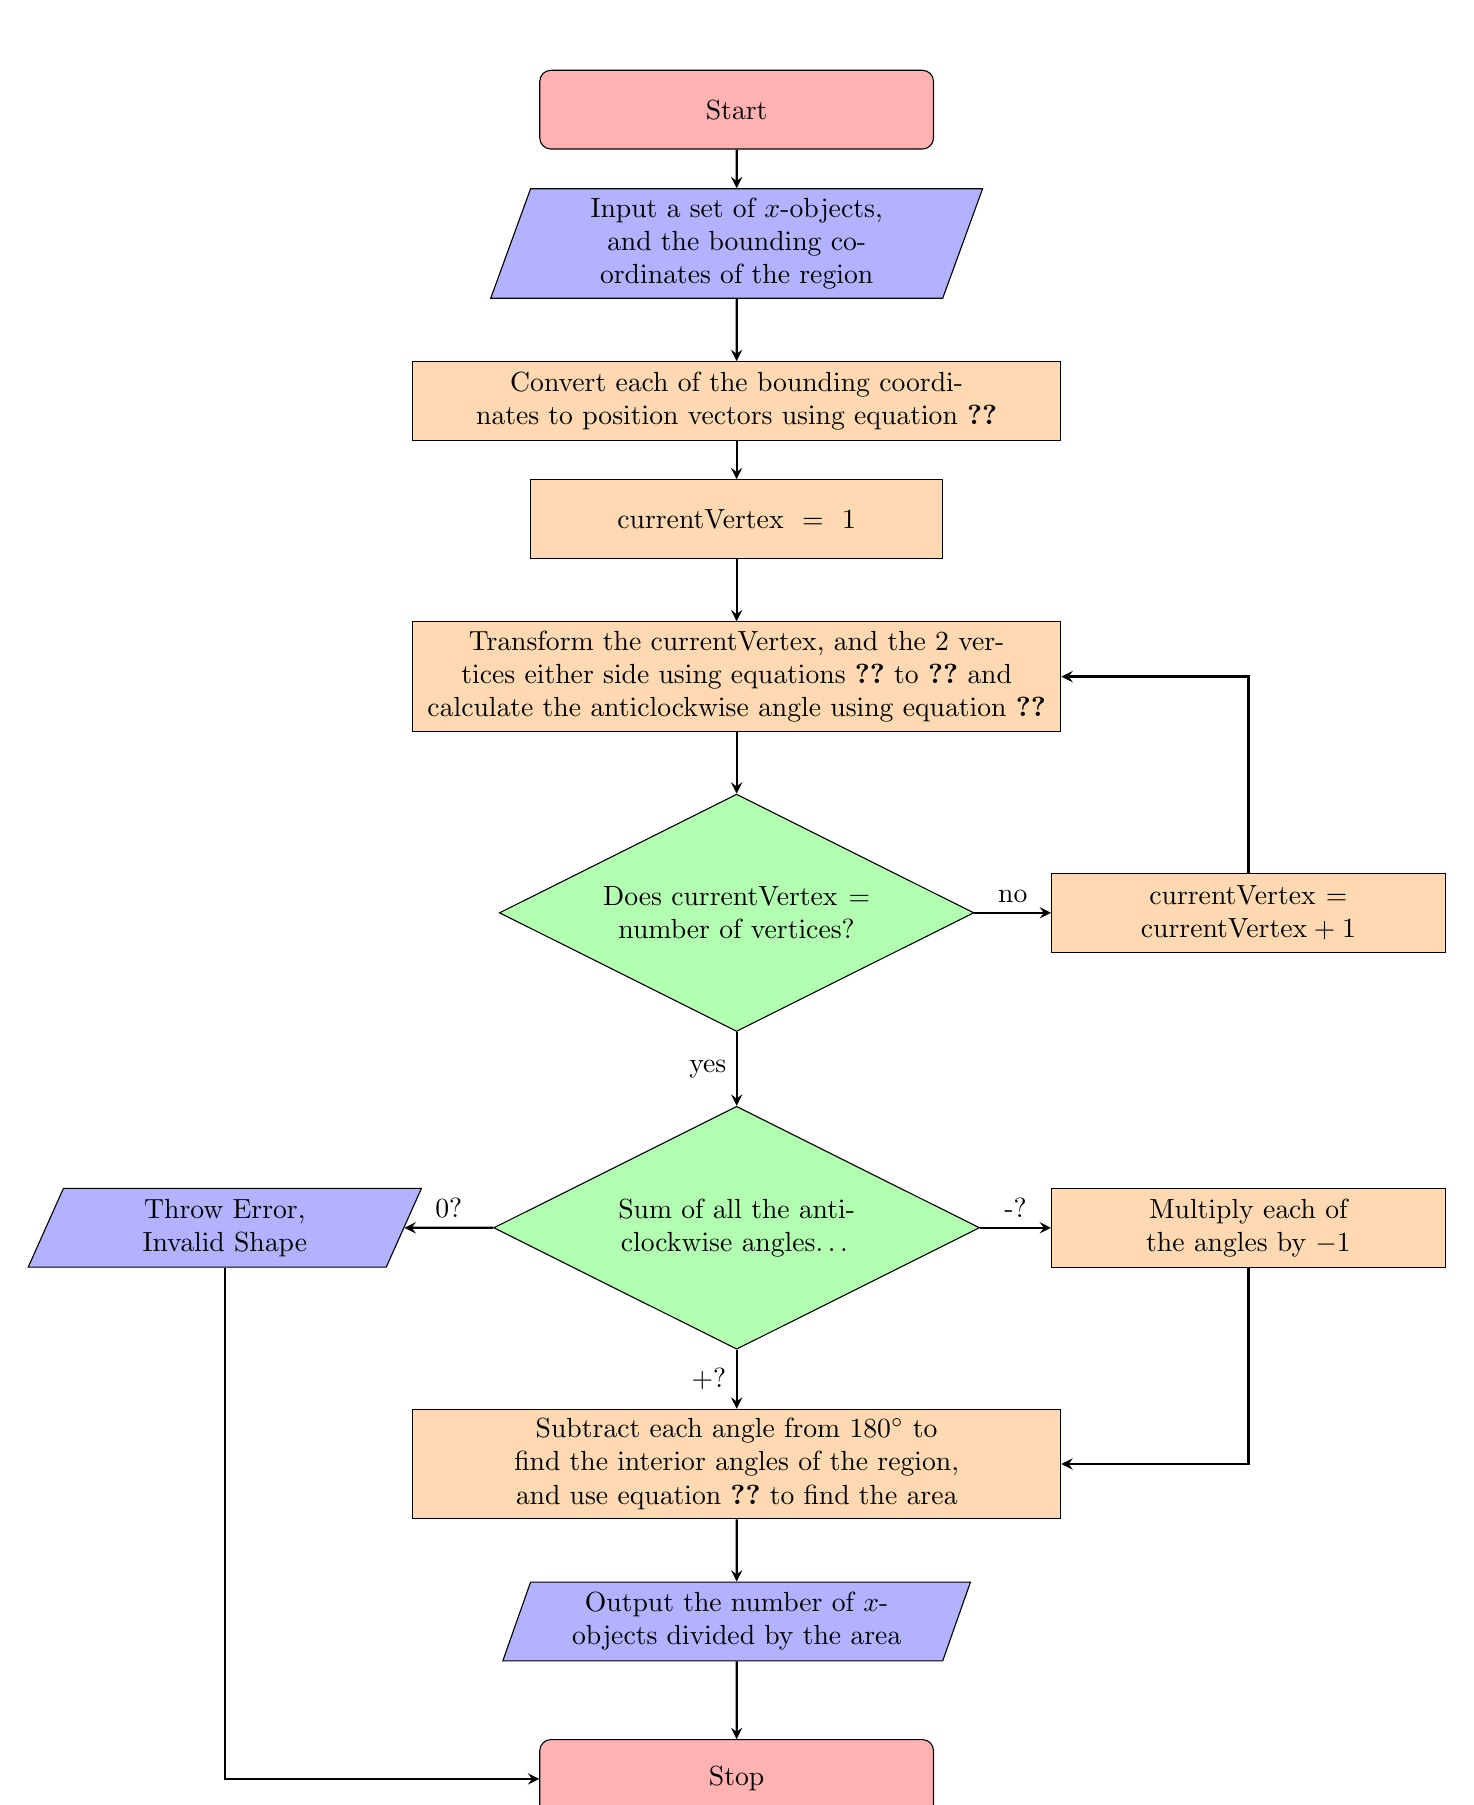
\begin{tikzpicture}[node distance=2cm]
    \node (start) [fStartStop] {Start};
    \node (instuff) [fInputOutput, below of=start, yshift=0.3cm] {Input a set of $x$-objects, and the bounding coordinates of the region};
    \node (convert2vectors) [fProcess, below of=instuff, text width=8cm] {Convert each of the bounding coordinates to position vectors using equation \ref{eq:convert2vectors}};
    \node (vertex1) [fProcess, below of=convert2vectors, yshift=0.5cm] {$\text{currentVertex}=1$};
    \node (transform) [fProcess, below of=vertex1, text width=8cm] {Transform the currentVertex, and the 2 vertices either side using equations \ref{eq:transformCoordsStart} to \ref{eq:transformCoordsEnd} and calculate the anticlockwise angle using equation \ref{eq:calcClockwiseAngle}};
    \node (decision) [fDecision, below of=transform, yshift=-1cm] {Does $\text{currentVertex}=\text{number of vertices}$?};
    \node (incrementVertex) [fProcess, right of=decision, xshift=4.5cm, text width=3cm] {$\text{currentVertex}=\text{currentVertex}+1$};
    \node (totalClockwise) [fDecision, below of=decision, yshift=-2cm] {Sum of all the anticlockwise angles\ldots};
    \node (outInvalid) [fInputOutput, left of=totalClockwise, xshift=-4.5cm, text width=3cm] {Throw Error, Invalid Shape};
    \node (negative) [fProcess, right of=totalClockwise, xshift=4.5cm, text width=3cm] {Multiply each of the angles by $-1$};
    \node (calcArea) [fProcess, below of=totalClockwise, yshift=-1cm, text width=8cm] {Subtract each angle from $180^{\circ}$ to find the interior angles of the region, and use equation \ref{eq:areaRegion} to find the area};
    \node (out) [fInputOutput, below of=calcArea] {Output the number of $x$-objects divided by the area};
    \node (stop) [fStartStop, below of=out] {Stop};
    
    \draw [fArrow] (start) -- (instuff);
    \draw [fArrow] (instuff) -- (convert2vectors);
    \draw [fArrow] (convert2vectors) -- (vertex1);
    \draw [fArrow] (vertex1) -- (transform);
    \draw [fArrow] (transform) -- (decision);
    \draw [fArrow] (decision) -- node[anchor=east] {yes} (totalClockwise);
    \draw [fArrow] (decision) -- node[anchor=south] {no} (incrementVertex);
    \draw [fArrow] (incrementVertex) |- (transform);
    \draw [fArrow] (totalClockwise) -- node[anchor=south] {0?} (outInvalid);
    \draw [fArrow] (totalClockwise) -- node[anchor=south] {-?} (negative);
    \draw [fArrow] (totalClockwise) -- node[anchor=east] {+?} (calcArea);
    \draw [fArrow] (negative) |- (calcArea);
    \draw [fArrow] (calcArea) -- (out);
    \draw [fArrow] (out) -- (stop);
    \draw [fArrow] (outInvalid) |- (stop);
\end{tikzpicture}
\caption{$D\left(x\right)$ Flowchart}\label{fig:dofx}
\end{figure}

\subsection{Overall Algorithm for Data Collection \& Processing}\label{sec:dataCollectionFullAlgo}
In order to train a neural network, I need both input and output data. The input data will be 24 factors listed above, in section \ref{sec:listOfFactors}, and the output data will be the true HDI of the region.

For this, I will be using the subnational region data from the Global Data Lab \cite{hdiData}, in order to maximise the number of training examples. In order to calculate the 24 factors for each of these regions, I will need the bounding coordinates of all the regions. I will also get this data from the Global Data Lab \cite{regionBorders}, which contains shapefile data on all of the subnational regions.

Therefore, all we need to do is for each subnational region, calculate each factor and store it in an external file (e.g a \pil{.csv} file) along with the correct HDI, ready for the neural network to train on.

In order to calculate each factor however, we must first query Overpass Turbo, in order to get the data about the locations objects.
\begin{figure}[H]
\centering
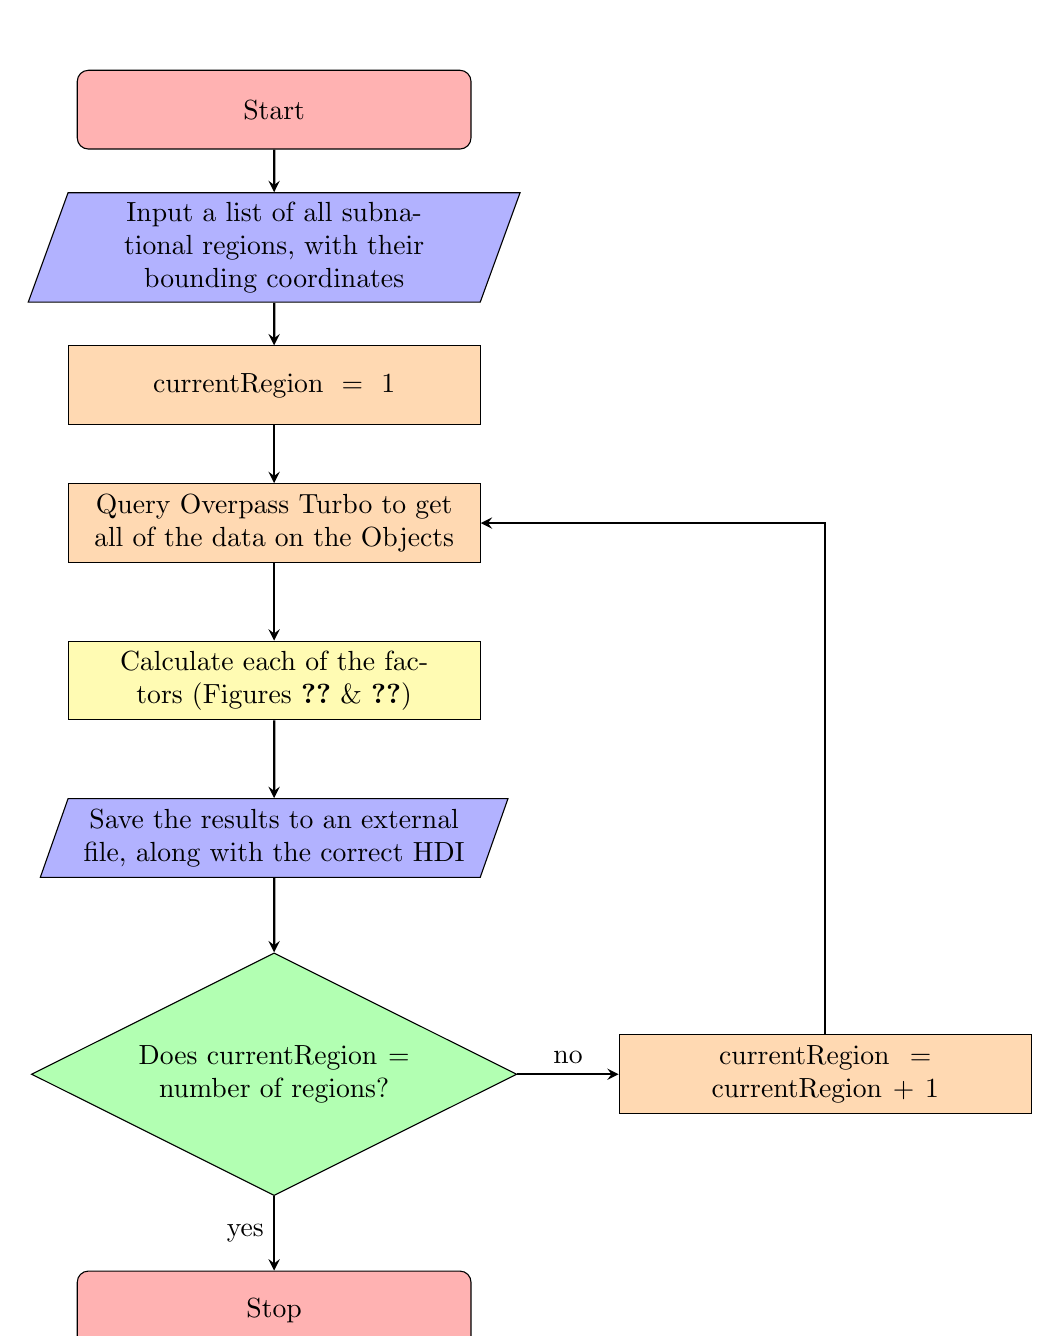
\begin{tikzpicture}[node distance=2cm]
    \node (start) [fStartStop] {Start};
    \node (inRegions) [fInputOutput, below of=start, yshift=0.25cm] {Input a list of all subnational regions, with their bounding coordinates};
    \node (region0) [fProcess, below of=inRegions, yshift=0.25cm] {$\text{currentRegion}=1$};
    \node (overpassTurbo) [fProcess, below of=region0, yshift=0.25cm] {Query Overpass Turbo to get all of the data on the Objects};
    \node (calcFactors) [fSubprocess, below of=overpassTurbo] {Calculate each of the factors (Figures \ref{fig:aofxy} \& \ref{fig:dofx})};
    \node (out) [fInputOutput, below of=calcFactors] {Save the results to an external file, along with the correct HDI};
    \node (decision) [fDecision, below of=out, yshift=-1cm] {Does $\text{currentRegion}=\text{number of regions}$?};
    \node (incrementRegion) [fProcess, right of=decision, xshift=5cm] {$\text{currentRegion}=\text{currentRegion}+1$};
    \node (stop) [fStartStop, below of=decision, yshift=-1cm] {Stop};
    
    \draw [fArrow] (start) -- (inRegions);
    \draw [fArrow] (inRegions) -- (region0);
    \draw [fArrow] (region0) -- (overpassTurbo);
    \draw [fArrow] (overpassTurbo) -- (calcFactors);
    \draw [fArrow] (calcFactors) -- (out);
    \draw [fArrow] (out) -- (decision);
    \draw [fArrow] (decision) -- node[anchor=east] {yes} (stop);
    \draw [fArrow] (decision) -- node[anchor=south] {no} (incrementRegion);
    \draw [fArrow] (incrementRegion) |- (overpassTurbo);
\end{tikzpicture}
\caption{Overall Data Collection \& Processing Algorithm Flowchart}
\end{figure}

\subsection{List of Key Variables}
\subsubsection{Variables in $A\left(x,y\right)$}
\begin{center}
\begin{longtable}{ | m{3cm} | m{4cm}| m{4cm} | m{4cm} |} 
    \hline
    \textbf{Identifier} & \textbf{Data Type} & \textbf{Explanation}  & \textbf{Justification} \\ 
    \hline
    \pil{x_objects} & \pil{list[tuple[float]]} & Parameter of the function, holds a list of the coordinates of all the $x$-objects. & Each coordinate is a tuple as the latitudes and longitudes will never change. \\ 
    \hline
    \pil{y_objects} & \pil{list[tuple[float]]} & Parameter of the function, holds a list of the coordinates of all the $y$-objects. & Each coordinate is a tuple as the latitudes and longitudes will never change. \\ 
    \hline
    \pil{max_x_objects} & \pil{int} & Parameter of the function, holds the maximum number of $x$-object to consider. Was 500 in the explanation above. & Considering every $x$-object would take a long time, and so some random sampling must be done. \\ 
    \hline
    \pil{x_object} & \pil{tuple[float]} & Iterator variable for when looping through \pil{x_objects}. & Is the singular of \pil{x_objects}. \\ 
    \hline
    \pil{y_object} & \pil{tuple[float]} & Iterator variable for when looping through \pil{y_objects}. & Is the singular of \pil{y_objects}. \\ 
    \hline
    \pil{dists_to_ys} & \pil{list[float]} & Holds the distances to each $y$-object for a particular $x$-object. & We must use this to find the minimum distance out of the distances stored. \\ 
    \hline
    \pil{min_dists} & \pil{list[float]} & Holds the minimum distances from each $x$-object to the nearest $y$-object. & $A\left(x,y\right)$ is given by the average of this list. \\ 
    \hline
\caption{List of Key Variables in $A\left(x,y\right)$}
\end{longtable}
\end{center}

\subsubsection{Variables in $D\left(x\right)$}
\begin{center}
\begin{longtable}{ | m{3cm} | m{4cm}| m{4cm} | m{4cm} |} 
    \hline
    \textbf{Identifier} & \textbf{Data Type} & \textbf{Explanation}  & \textbf{Justification} \\ 
    \hline
    \pil{x_objects} & \pil{list[tuple[float]]} & Parameter of the function, holds a list of the coordinates of all the $x$-objects. & Each coordinate is a tuple as the latitudes and longitudes will never change. \\ 
    \hline
    \pil{bounding_coords} & \pil{list[tuple[float]]} & Parameter of the function, holds a list of the bounding coordinates of the region. & Each coordinate is a tuple as the latitudes and longitudes will never change. \\ 
    \hline
    \pil{bounding_vectors} & \pil{list[column_vector]} & Holds the \pil{bounding_coords} once converted into column vectors. & This is so that we can use matrix multiplication to rotate them. \\ 
    \hline
    \pil{current_vertex} & \pil{int} & Iterator variable to keep track of which vertex I am dealing with. & Use it to get the vertex from the \pil{bounding_vectors} as well as the previous and next one. \\ 
    \hline
    \pil{transformed_vertices} & \pil{list[column_vector]} & Holds the transformed \pil{current_vertex} as well as the prevous and next one. & We must compute the vectors and anticlockwise angles from this. \\ 
    \hline
    \pil{anticlockwise_angles} & \pil{list[float]} & Holds all of the anticlockwise angles at each vertex. & We need to sum this to determine if they are actually anticlockwise angles or not. \\ 
    \hline
    \pil{interior_angles} & \pil{list[float]} & Holds the interior angles of the region the user has drawn. & This is one of the terms in the formula to calculate the area of the region. \\ 
    \hline
    \pil{area} & \pil{float} & Holds the area of the region the user has drawn. & $D\left(x\right)$ is given by the length of \pil{x_objects} divided by this. \\ 
    \hline
\caption{List of Key Variables in $D\left(x\right)$}
\end{longtable}
\end{center}

The data structure \pil{column_vector} does not come with python, but can be implemented with the \pil{numpy} module.

\subsubsection{Other Variables}
\begin{center}
\begin{longtable}{ | m{3cm} | m{4cm}| m{4cm} | m{4cm} |} 
    \hline
    \textbf{Identifier} & \textbf{Data Type} & \textbf{Explanation}  & \textbf{Justification} \\ 
    \hline
    \pil{current_region} & \pil{int} & Iterator variable for iterating through the regions. & We must calculate all of the factors for each region. \\ 
    \hline
    \pil{dataset_path} & \pil{str} & Stores the file path to the external file for which the neural network will read the data from. & The neural network may need to be trained more than once, due to mistakes, so storing this in an external file would be beneficial. \\ 
    \hline
\caption{List of Other Key Variables in Data Collection \& Processing}
\end{longtable}
\end{center}

As the user never interacts with this part of the program, there is no validation that needs to be done (e.g. as stuff is automatically in the right type).

\section{Multilayer Perceptron}\label{sec:mlp}
All the information in this section, I learned from 3blue1brown's videos \cite{3blue1brown} and Micheal Nielsen's e-book \cite{backpropogation} on the topic.
\subsection{Structure}\label{sec:mlpStruct}
\subsubsection{Layers \& Neurons}
The structure of a multilayer perceptron is similar to that of a graph, in the sense that it has a series of nodes (neurons) and edges (weights). The neurons are arranged in layers, the first of which being the input layer, the last being the output layer, and any in between being hidden layers.
\begin{figure}[H]
\centering
\begin{neuralnetwork}[nodespacing=15mm,layerspacing=30mm]
\inputlayer[count=5, title=Input Layer, text=\nodetext, bias=false]
\hiddenlayer[count=4, title=Hidden Layer 1, text=\nodetext, bias=false] \linklayers
\hiddenlayer[count=4, title=Hidden Layer 2, text=\nodetext, bias=false] \linklayers
\outputlayer[count=1, title=Output Layer, text=\nodetext, bias=false] \linklayers
\end{neuralnetwork}
\caption{Neural Network Structure}\label{fig:nnStructure}
\end{figure}

Figure \ref{fig:nnStructure} shows an example neural network, with 5 neurons in the input layer (shown in green), 1 neuron in the output layer (shown in red), and 2 hidden layers each with 4 neurons (shown in blue). ``Multilayer Perceptron'' is just the fancy official name for this type of machine learning model.

Each neuron will hold a number, which will represent something. In the input layer, the neurons represent the various inputs to the system. In my case, they will be the various factors that may affect the HDI, so my neural network will have 24 neurons in the input layer. In the output layer, the neuron(s) will represent whatever output the system should have. For example, I only want 1 output, the HDI, so there is 1 neuron in the output layer which will hold the predicted HDI.

In the hidden layers, the hope is that the neurons will represent something intermediate in between the input and the output. For example, if the input neurons represent geographical factors, and the output neuron represents the HDI, the neurons in hidden layer 1 might represent the \textit{gist} of how good the schooling is, or how good the healthcare is, and the neurons in hidden layer 2 might represent the \textit{gist} of how these things work together to result in a higher HDI. This means that the original problem of calculating HDI from a set of factors has been decomposed into a series of smaller tasks.

As shown in Figure \ref{fig:nnStructure}, I will use the notation $a^{\left(l\right)}_i$ to denote a particular neuron, where $l$ is the index of the layer that it is in, and $i$ is its index within the layer. In general, a network will have $L$ layers, not including the input layer (as the layers are 0-indexed).
\subsubsection{Weights}
The value of each neuron (that isn't in the input layer) should be based on all the neurons of the previous layer, as shown by the arrows in Figure \ref{fig:nnStructure}.
\begin{figure}[H]
\centering
\begin{neuralnetwork}[nodespacing=15mm,layerspacing=30mm]
\inputlayer[count=5, title=Input Layer, text=\nodetext, bias=false]
\hiddenlayer[count=4, title=Hidden Layer 1, text=\nodetext, bias=false] \linklayers
\hiddenlayer[count=4, title=Hidden Layer 2, text=\nodetext, bias=false] \linklayers
\outputlayer[count=1, title=Output Layer, text=\nodetext, bias=false] \linklayers
\link[style={black}, labelpos=near start, from layer=0, to layer=1, from node=1, to node=2, label=\weighttext]
\link[style={black}, labelpos=near start, from layer=0, to layer=1, from node=2, to node=2, label=\weighttext]
\link[style={black}, labelpos=near start, from layer=0, to layer=1, from node=3, to node=2, label=\weighttext]
\link[style={black}, labelpos=near start, from layer=0, to layer=1, from node=4, to node=2, label=\weighttext]
\link[style={black}, labelpos=near start, from layer=0, to layer=1, from node=5, to node=2, label=\weighttext]
\link[style={black}, labelpos=near end, from layer=1, to layer=2, from node=2, to node=1, label=\weighttext]
\link[style={black}, labelpos=near end, from layer=1, to layer=2, from node=2, to node=2, label=\weighttext]
\link[style={black}, labelpos=near end, from layer=1, to layer=2, from node=2, to node=3, label=\weighttext]
\link[style={black}, labelpos=near end, from layer=1, to layer=2, from node=2, to node=4, label=\weighttext]
\end{neuralnetwork}
\caption{Neural Network Weights}\label{fig:nnWeights}
\end{figure}

I will use the notation $w^{\left(l\right)}_{i,j}$ to denote a particular weight, where $l$ is the index of the layer it is pointing from, $i$ is the neuron's index within its layer that the weight is pointing to, and $j$ is the neuron's index within its layer that the weight is pointing from, as shown in Figure \ref{fig:nnWeights}.

Each weight will also hold a value (any real number), which will not be calculated during prediction (like neurons' values are), and so the weights are parameters of the system. Initially, they will be set to random values, which will change during training.

\subsection{Feedforward Algorithm \& Prediction}\label{sec:feedforward}
\subsubsection{Weighted Sum}
Again, the value of each neuron (that isn't in the input layer) should be based on all the neurons of the previous layer. This can be done using a weighted sum. For example, the equation to calculate the value of $a^{\left(1\right)}_1$ in this example neural network would be:
\begin{equation}
    a^{\left(1\right)}_1=w^{\left(0\right)}_{1,1}a^{\left(0\right)}_1+w^{\left(0\right)}_{1,2}a^{\left(0\right)}_2+w^{\left(0\right)}_{1,3}a^{\left(0\right)}_3+w^{\left(0\right)}_{1,4}a^{\left(0\right)}_4+w^{\left(0\right)}_{1,5}a^{\left(0\right)}_5
\end{equation}
\begin{figure}[H]
\centering
\begin{neuralnetwork}[nodespacing=15mm,layerspacing=30mm]
\inputlayer[count=5, title=Input Layer, text=\nodetext, bias=false]
\hiddenlayer[count=4, title=Hidden Layer 1, text=\nodetext, bias=false] \linklayers
\hiddenlayer[count=4, title=Hidden Layer 2, text=\nodetext, bias=false] \linklayers
\outputlayer[count=1, title=Output Layer, text=\nodetext, bias=false] \linklayers
\link[style={black}, labelpos=near start, from layer=0, to layer=1, from node=1, to node=1, label=\weighttext]
\link[style={black}, labelpos=near start, from layer=0, to layer=1, from node=2, to node=1, label=\weighttext]
\link[style={black}, labelpos=near start, from layer=0, to layer=1, from node=3, to node=1, label=\weighttext]
\link[style={black}, labelpos=near start, from layer=0, to layer=1, from node=4, to node=1, label=\weighttext]
\link[style={black}, labelpos=near start, from layer=0, to layer=1, from node=5, to node=1, label=\weighttext]
\end{neuralnetwork}
\caption{Calculating $a^{\left(1\right)}_1$ Example}
\end{figure}

In general, the equation to calculate the value of some neuron $a^{\left(l\right)}_i$ in any given network would be:
\begin{equation}
    a^{\left(l\right)}_i=w^{\left(l-1\right)}_{i,1}a^{\left(l-1\right)}_1+w^{\left(l-1\right)}_{i,2}a^{\left(l-1\right)}_2+w^{\left(l-1\right)}_{i,3}a^{\left(l-1\right)}_3+\cdots +w^{\left(l-1\right)}_{i,n}a^{\left(l-1\right)}_n
\end{equation}
where $n$ is the number of neurons in layer $l-1$ (the previous layer).

\subsubsection{Activation Function}
The value of each neuron should also represent how ``activated'' that neuron is, ideally on a continuous scale from 0 to 1. This is to match what happens in biological neural networks (brains), as this is effectively a model for that. The 0 to 1 range is also suitable in this particular instance, as HDI is also measured on a continuous scale from 0 to 1.

However, the result of this weighted sum could be any real number (as the weights can be any real number), so in order to squish it into the 0 to 1 range, it must be passed through some function, the activation function.

There are many activation functions that could be used, but the one I will use is $\sigma \left(x\right)$ (``sigmoid of $x$''), which is defined as:
\begin{equation}\label{eq:sigmoid}
    \sigma \left(x\right)=\frac{1}{1+e^{-x}}
\end{equation}

Why this is suitable is best shown in the graph of $y=\sigma \left(x\right)$:
\begin{figure}[H]
\centering
\begin{tikzpicture}
\begin{axis}[
    axis lines=middle,
    axis line style={-stealth,shorten >=-3mm},
    ymax=1,
    xlabel = $x$,
    ylabel = $y$,
    width=\columnwidth,
    height=2in,
    scale only axis
]
\addplot[
    domain=-8:8,
    samples=100,
    red
]{1/(1+e^(-x))};
\end{axis}
\end{tikzpicture}
\caption{Graph of $y=\sigma \left(x\right)$}\label{fig:sigmoidX}
\end{figure}

As shown in Figure \ref{fig:sigmoidX}, the domain of $\sigma \left(x\right)$ is $\mathbb{R}$ (all real numbers), which is what the evaluation of the weighted sum could be, and the range is $0<\sigma \left(x\right)<1$, which is what we want it to be. Therefore, if the weighted sum is negative, then the activation of the neuron (its value) will be between 0 and 0.5, and if the weighted sum is positive, its activation will be between 0.5 and 1.

As the graph has asymptotes at $y=0$ and $y=1$ (which means that the function approaches it but never reaches it), very negative weighted sums will result in activations $\approx 0$, and very positive weighted sums will result in activations $\approx 1$. The smooth curve in the middle will also mean that the change from 0 to 1 is gradual, and there are no sudden jumps. (The function is also differentiable on its entire domain, which will be helpful in the Backpropogation Algorithm).

Therefore, the equation to calculate the activation of some neuron $a^{\left(l\right)}_i$ in any given network would now be:
\begin{equation}
    a^{\left(l\right)}_i=\sigma \left(w^{\left(l-1\right)}_{i,1}a^{\left(l-1\right)}_1+w^{\left(l-1\right)}_{i,2}a^{\left(l-1\right)}_2+w^{\left(l-1\right)}_{i,3}a^{\left(l-1\right)}_3+\cdots +w^{\left(l-1\right)}_{i,n}a^{\left(l-1\right)}_n\right)
\end{equation}
where $n$ is the number of neurons in layer $l-1$.

\subsubsection{Bias}
A neuron may be considered ``activated'' if its value is $\geq 0.5$. For now, this is where the weighted sum is $\geq 0$, as $\sigma \left(0\right)=0.5$. But what if a particular neuron should be activated when the weighted sum is (for examle) $\geq 5$, or $\geq -87.2$?

To achieve this, each neuron (that isn't in the input layer) has a bias, which is another real number which is added onto the weighted sum before the activation function. I will use the notation $b^{\left(l\right)}_i$ to denote the bias of neuron $a^{\left(l\right)}_i$. The biases (like the weights) are also parameters of the system.

\begin{figure}[H]
\centering
\begin{tikzpicture}
\begin{axis}[
    axis lines=middle,
    axis line style={-stealth,shorten >=-3mm},
    ymax=1,
    xlabel = $x$,
    ylabel = $y$,
    width=\columnwidth,
    height=2in,
    scale only axis
]
\addplot[
    domain=-10:6,
    samples=100,
    red
]{1/(1+e^(-(x+2)))};
\end{axis}
\end{tikzpicture}
\caption{Graph of $y=\sigma \left(x+2\right)$}\label{fig:sigmoidXplus2}
\end{figure}

Figure \ref{fig:sigmoidXplus2} shows the graph of $y=\sigma \left(x+2\right)$, which shows how a particular neuron would be activated if its weighted sum is $\geq -2$.

Therefore, if a particular neuron $a^{\left(l\right)}_i$ should be activated if its weighted sum is $\geq p$, then $b^{\left(l\right)}_i=-p$. However, we have no way of knowing what this value of $p$ should be for any of the neurons in the network, as what the neurons represent are too abstract for us to understand. Like the weights, they will be initially set to random values, and will change during training.

The final equation to calculate the activation of some neuron $a^{\left(l\right)}_i$ in any given network is:
\begin{equation}\label{eq:activationofaneuron}
    a^{\left(l\right)}_i=\sigma \left(w^{\left(l-1\right)}_{i,1}a^{\left(l-1\right)}_1+w^{\left(l-1\right)}_{i,2}a^{\left(l-1\right)}_2+w^{\left(l-1\right)}_{i,3}a^{\left(l-1\right)}_3+\cdots +w^{\left(l-1\right)}_{i,n}a^{\left(l-1\right)}_n+b^{\left(l\right)}_i\right)
\end{equation}
where $n$ is the number of neurons in layer $l-1$.

\subsubsection{Rearranging into Matrices \& Column Vectors}
Instead of calculating the activation of each neuron 1 by 1, consider calculating an entire layer of neurons at once. 
\begin{figure}[H]
\centering
\begin{neuralnetwork}[nodespacing=15mm,layerspacing=30mm]
\inputlayer[count=5, title=Input Layer, text=\nodetext, bias=false]
\hiddenlayer[count=4, title=Hidden Layer 1, text=\nodetext, bias=false] \linklayers[style={black}]
\hiddenlayer[count=4, title=Hidden Layer 2, text=\nodetext, bias=false] \linklayers
\outputlayer[count=1, title=Output Layer, text=\nodetext, bias=false] \linklayers
\end{neuralnetwork}
\caption{Calculating an entire layer of neurons}
\end{figure}

To do this, we can arrange each layer of neurons and their biases into column vectors (transposed arrays), $\mathbf{a}^{\left(l\right)}$ and $\mathbf{b}^{\left(l\right)}$ respectively, where $l$ is the index of their layer:
\begin{equation}
    \mathbf{a}^{\left(l\right)}=\begin{pmatrix}a^{\left(l\right)}_1\\[0.3em]a^{\left(l\right)}_2\\\vdots \\a^{\left(l\right)}_n\end{pmatrix},\mathbf{b}^{\left(l\right)}=\begin{pmatrix}b^{\left(l\right)}_1\\[0.3em]b^{\left(l\right)}_2\\\vdots \\b^{\left(l\right)}_n\end{pmatrix}
\end{equation}
where $n$ is the number of neurons in layer $l$.

Arrange the weights in between each layer into a matrix (2D array), $\mathbf{W}^{\left(l\right)}$, where $l$ is the layer the weights are pointing from:
\begin{equation}
    \mathbf{W}^{\left(l\right)}=\begin{pmatrix}w^{\left(l\right)}_{1,1}&w^{\left(l\right)}_{1,2}&\cdots&w^{\left(l\right)}_{1,n}\\[0.3em]w^{\left(l\right)}_{2,1}&w^{\left(l\right)}_{2,2}&\cdots&w^{\left(l\right)}_{2,n}\\\vdots&\vdots&\ddots&\vdots\\w^{\left(l\right)}_{m,1}&w^{\left(l\right)}_{m,2}&\cdots&w^{\left(l\right)}_{m,n}\end{pmatrix}
\end{equation}
where $n$ is the number of neurons in layer $l$ and $m$ is the number of neurons in layer $l+1$.

Consider the matrix multiplication, $\mathbf{W}^{\left(l\right)}\mathbf{a}^{\left(l\right)}$:
\begin{equation}
    \begin{pmatrix}w^{\left(l\right)}_{1,1}&w^{\left(l\right)}_{1,2}&\cdots&w^{\left(l\right)}_{1,n}\\[0.3em]w^{\left(l\right)}_{2,1}&w^{\left(l\right)}_{2,2}&\cdots&w^{\left(l\right)}_{2,n}\\\vdots&\vdots&\ddots&\vdots\\w^{\left(l\right)}_{m,1}&w^{\left(l\right)}_{m,2}&\cdots&w^{\left(l\right)}_{m,n}\end{pmatrix}\begin{pmatrix}a^{\left(l\right)}_1\\[0.3em]a^{\left(l\right)}_2\\\vdots \\a^{\left(l\right)}_n\end{pmatrix}=\begin{pmatrix}w^{\left(l\right)}_{1,1}a^{\left(l\right)}_1+w^{\left(l\right)}_{1,2}a^{\left(l\right)}_2+\cdots +w^{\left(l\right)}_{1,n}a^{\left(l\right)}_n\\[0.3em]w^{\left(l\right)}_{2,1}a^{\left(l\right)}_1+w^{\left(l\right)}_{2,2}a^{\left(l\right)}_2+\cdots +w^{\left(l\right)}_{2,n}a^{\left(l\right)}_n\\\vdots\\w^{\left(l\right)}_{m,1}a^{\left(l\right)}_1+w^{\left(l\right)}_{m,2}a^{\left(l\right)}_2+\cdots +w^{\left(l\right)}_{m,n}a^{\left(l\right)}_n\end{pmatrix}
\end{equation}
The result is a column vector, where each item is a weighted sum of all the neurons in that layer, which is almost the correct column vector for the activations of the neurons in the next layer! To make it correct, we just need to add the bias column vector for the next layer, and pass it through the activation function.

Therefore, the equation to calculate the activations of all the neurons in the next layer, $l+1$ is:
\begin{equation}
    \begin{pmatrix}a^{\left(l+1\right)}_1\\[0.3em]a^{\left(l+1\right)}_2\\\vdots \\a^{\left(l+1\right)}_m\end{pmatrix}=\sigma \left(\begin{pmatrix}w^{\left(l\right)}_{1,1}&w^{\left(l\right)}_{1,2}&\cdots&w^{\left(l\right)}_{1,n}\\[0.3em]w^{\left(l\right)}_{2,1}&w^{\left(l\right)}_{2,2}&\cdots&w^{\left(l\right)}_{2,n}\\\vdots&\vdots&\ddots&\vdots\\w^{\left(l\right)}_{m,1}&w^{\left(l\right)}_{m,2}&\cdots&w^{\left(l\right)}_{m,n}\end{pmatrix}\begin{pmatrix}a^{\left(l\right)}_1\\[0.3em]a^{\left(l\right)}_2\\\vdots \\a^{\left(l\right)}_n\end{pmatrix}+\begin{pmatrix}b^{\left(l+1\right)}_1\\[0.3em]b^{\left(l+1\right)}_2\\\vdots \\b^{\left(l+1\right)}_m\end{pmatrix}\right)
\end{equation}
where $n$ is the number of neurons in layer $l$, $m$ is the number of neurons in layer $l+1$ and $\sigma$ of a column vector $=\sigma$ of all the items in the column vector.

This can be simply written as:
\begin{equation}\label{eq:activationOfLayer}
    \mathbf{a}^{\left(l+1\right)}=\sigma \left(\mathbf{W}^{\left(l\right)}\mathbf{a}^{\left(l\right)}+\mathbf{b}^{\left(l+1\right)}\right)
\end{equation}
where $\sigma$ of a column vector $=\sigma$ of all the items in the column vector, which is the formula that I will be using in my program.

\subsubsection{Final Algorithm}
In order to fully make a prediction, we just need to iterate this process over all the layers:
\begin{figure}[H]
\centering
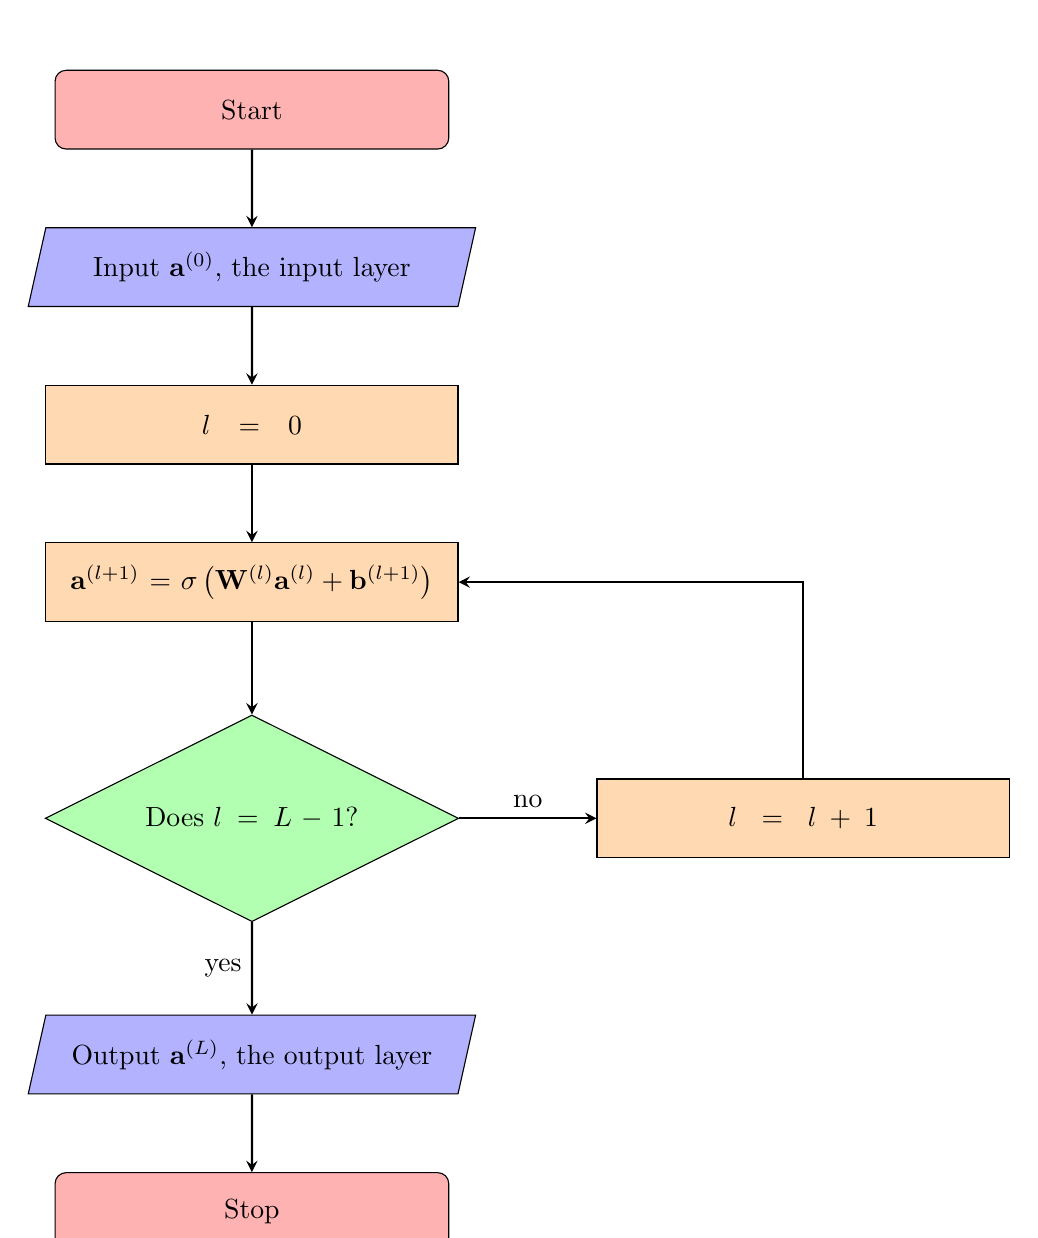
\begin{tikzpicture}[node distance=2cm]
    \node (start) [fStartStop] {Start};
    \node (ina0) [fInputOutput, below of=start] {Input $\mathbf{a}^{\left(0\right)}$, the input layer};
    \node (lequals0) [fProcess, below of=ina0] {$l=0$};
    \node (feedforward) [fProcess, below of=lequals0] {$\mathbf{a}^{\left(l+1\right)}=\sigma \left(\mathbf{W}^{\left(l\right)}\mathbf{a}^{\left(l\right)}+\mathbf{b}^{\left(l+1\right)}\right)$};
    \node (decision) [fDecision, below of=feedforward, yshift=-1cm] {Does $l=L-1$?};
    \node (incrementl) [fProcess, right of=decision, xshift=5cm] {$l=l+1$};
    \node (out) [fInputOutput, below of=decision, yshift=-1cm] {Output $\mathbf{a}^{\left(L\right)}$, the output layer};
    \node (stop) [fStartStop, below of=out] {Stop};
    
    \draw [fArrow] (start) -- (ina0);
    \draw [fArrow] (ina0) -- (lequals0);
    \draw [fArrow] (lequals0) -- (feedforward);
    \draw [fArrow] (feedforward) -- (decision);
    \draw [fArrow] (decision) -- node[anchor=east] {yes} (out);
    \draw [fArrow] (decision) -- node[anchor=south] {no} (incrementl);
    \draw [fArrow] (incrementl) |- (feedforward);
    \draw [fArrow] (out) -- (stop);
\end{tikzpicture}
\caption{Feedforward Algorithm Flowchart}\label{fig:feedforward}
\end{figure}

\subsection{Backpropogation Algorithm \& Training}\label{sec:backpropogation}
\subsubsection{The Cost Function \& Gradient Descent}
This feedforward algorithm to make predictions works, but if you were to test it right now it would return absolute nonsense. This is because all the weights and biases of the network are initially set to random values, so in reality the network isn't doing anything in particular. In order for it to recognise patterns within factors which may contribute to HDI, it must be trained on a set of examples. The network should also know after a prediction how far off it was from the correct answer.

Therefore, define the ``cost'' of a single example, $c$ to be: 
\begin{equation}\label{eq:cdefinition}
    c=\displaystyle\sum_{i=1}^{n}\frac{1}{2}{\left(a^{\left(L\right)}_i-y_i\right)}^2
\end{equation}
where $a^{\left(L\right)}_i$ is the activation of the $i^{\text{th}}$ neuron in the output layer, $y_i$ is the ``correct'' activation, as given by the training example, and $n$ is the number of neurons in layer $L$. As I will only have 1 neuron in the output layer, this simplifies to:
\begin{equation}
    c=\frac{1}{2}{\left(a^{\left(L\right)}_1-y\right)}^2
\end{equation}
where $a^{\left(L\right)}_1$ is the predicted HDI and $y$ is the true HDI. The difference between the true value and the predicted value is squared to always make it positive, as some predictions may be less than the true value and others may be greater than the true value.

Similarly to the activation function, there are many ways of defining the cost, $c$. I have chosen this one as it is simple to understand how it works, it is very quick to compute (as all you have to do is subtract 2 values, square and half) and it is differentiable on its entire domain, which will be helpful later.

Now define the cost function, $C$, to be the average cost over many pieces of training data, in terms of all the weights and biases:
\begin{equation}
    C\left(w^{\left(0\right)}_{1,1},\ldots ,w^{\left(L-1\right)}_{i,j},b^{\left(1\right)}_1,\ldots ,b^{\left(L\right)}_i\right)=\text{??? (depends on what the network does)}
\end{equation}
The goal is to find a minimum to this function, as when this function returns a small value, that means that all the predictions that the network gave were close to the true values.

We can do this by using gradient descent. This is where you find the gradient of the function, and then take a small step in the direction such that the gradient will decrease the most. This will work as the gradient at minimums of functions $=0$. In other words, we must find out how much each of the weights and biases affects the cost, and then using this information, change the weights and biases such that the cost will decrease.

\begin{figure}[H]
\centering
\begin{tikzpicture}
\begin{axis}[
    at={(0cm,0cm)},
    axis lines=middle,
    axis line style={-stealth,shorten >=-3mm},
    ymax=35,
    ymin=0,
    xlabel = $w$,
    ylabel = $C$,
    width=6cm,
    height=2in,
    scale only axis
]
\addplot[
    domain=-9:9,
    samples=100,
    red
]{((x+7)*(x+4)*(x+1)*(x-3)*(x-4)*(x-7))/1000+16};
\addplot[
    domain=-9:9,
    samples=100,
    blue
]{(1848/125)*x-(10936/125)};
\end{axis}
\draw[-stealth] (7,3) -- (9,3);
\begin{axis}[
    at={(10cm,0cm)},
    axis lines=middle,
    axis line style={-stealth,shorten >=-3mm},
    ymax=35,
    ymin=0,
    xlabel = $w$,
    ylabel = $C$,
    width=6cm,
    height=2in,
    scale only axis
]
\addplot[
    domain=-9:9,
    samples=100,
    red
]{((x+7)*(x+4)*(x+1)*(x-3)*(x-4)*(x-7))/1000+16};
\addplot[
    domain=-9:9,
    samples=100,
    blue
]{(15057/3200)*x-(246217/12800)};
\end{axis}
\end{tikzpicture}
\caption{Gradient Descent Example}\label{fig:gradientdescent}
\end{figure}
Figure \ref{fig:gradientdescent} shows how $C$ may vary with some weight $w$, and how gradient descent will be used to find a minimum of $C$ with respect $w$. Note that it may not converge on the absolute minimum, but it will converge onto some local minimum. 

\subsubsection{Error of a Neuron, ${\delta}^{\left(l\right)}_i$}
To do this, it will help to find out how much each neuron affects the output of the network, or the cost. This will be called the error of a neuron.

First, define $z^{\left(l\right)}_i$ to be neuron $a^{\left(l\right)}_i$'s activation before it was passed into the activation function:
\begin{equation}\label{eq:zdefinition}
    z^{\left(l\right)}_i=w^{\left(l-1\right)}_{i,1}a^{\left(l-1\right)}_1+w^{\left(l-1\right)}_{i,2}a^{\left(l-1\right)}_2+w^{\left(l-1\right)}_{i,3}a^{\left(l-1\right)}_3+\cdots +w^{\left(l-1\right)}_{i,n}a^{\left(l-1\right)}_n+b^{\left(l\right)}_i
\end{equation}
Now we can define the error of a neuron $a^{\left(l\right)}_i$, ${\delta}^{\left(l\right)}_i$ to be:
\begin{equation}
    {\delta}^{\left(l\right)}_i=\diff{C}{z^{\left(l\right)}_i}
\end{equation}
which represents the quantity answered by the question: \textit{``If I make a tiny change to $z^{\left(l\right)}_i$, $\Delta z^{\left(l\right)}_i$ what is the resulting change in $C$?''}.

If ${\delta}^{\left(l\right)}_i$, is close to 0, there isn't much we can do to $z^{\left(l\right)}_i$ to have a big effect on $C$. On the other hand, if ${\delta}^{\left(l\right)}_i$ is large, then we only have to change $z^{\left(l\right)}_i$ a little bit to have a big effect on $C$. Therefore, there is a heuristic sense of how ${\delta}^{\left(l\right)}_i$ measures the sensitivity, or error, of a neuron.

The plan is to find the error of the output layer, then backpropogate that to find the error of previous layers, and finally find the change in the cost function $C$ with respect to the weights and biases in terms of these errors.

\subsubsection{Error of the Output Layer, $\bm{\delta}^{\left(L\right)}$}
The error of the neurons in the output layer will therefore be given by:
\begin{equation}
    {\delta}^{\left(L\right)}_i=\diff{C}{z^{\left(L\right)}_i}
\end{equation}
as $L$ is the number of layers in the network (not including the input layer), and therefore represents the output layer. However, this is not easily computable, and should be rearranged into something that is.

We can break up this expression using the chain rule for differentiation:
\begin{equation}\label{eq:chainrule}
    {\delta}^{\left(L\right)}_i=\diff{C}{a^{\left(L\right)}_i}\diff{a^{\left(L\right)}_i}{z^{\left(L\right)}_i}
\end{equation}

As $a^{\left(l\right)}_i=\sigma \left(z^{\left(l\right)}_i\right)$ by definition (from equations \ref{eq:activationofaneuron} and \ref{eq:zdefinition}),
\begin{equation}\label{eq:dabydz}
    \diff{a^{\left(L\right)}_i}{z^{\left(L\right)}_i}={\sigma}^{\prime} \left(z^{\left(L\right)}_i\right)
\end{equation}
where ${\sigma}^{\prime} \left(x\right)$ is the derivative of the sigmoid function.

As the output of $C$ is given by $\displaystyle\sum_{i=1}^{n}\frac{1}{2}{\left(a^{\left(L\right)}_i-y_i\right)}^2$ by definition (from equation \ref{eq:cdefinition}),
\begin{equation}\label{eq:dcbyda}
    \diff{C}{a^{\left(L\right)}_i}=a^{\left(L\right)}_i-y_i
\end{equation}

Therefore, from equations \ref{eq:chainrule}, \ref{eq:dabydz} and \ref{eq:dcbyda},
\begin{equation}
    {\delta}^{\left(L\right)}_i=\left(a^{\left(L\right)}_i-y_i\right)\left({\sigma}^{\prime} \left(z^{\left(L\right)}_i\right)\right)
\end{equation}
which is all easily computable.

As done before with $\mathbf{a}^{\left(l\right)}$ and $\mathbf{b}^{\left(l\right)}$, arrange each of the $z$-values and errors into column vectors, $\mathbf{z}^{\left(l\right)}$ and $\bm{\delta}^{\left(l\right)}$, where $l$ is the index of their layer:
\begin{equation}
    \mathbf{z}^{\left(l\right)}=\begin{pmatrix}z^{\left(l\right)}_1\\[0.3em]z^{\left(l\right)}_2\\\vdots \\z^{\left(l\right)}_n\end{pmatrix},\bm{\delta}^{\left(l\right)}=\begin{pmatrix}{\delta}^{\left(l\right)}_1\\[0.3em]{\delta}^{\left(l\right)}_2\\\vdots \\{\delta}^{\left(l\right)}_n\end{pmatrix}
\end{equation}
where $n$ is the number of neurons in layer $l$.

$\bm{\delta}^{\left(L\right)}$ must therefore be given by:
\begin{equation}\label{eq:errorOutputLayer}
    \bm{\delta}^{\left(L\right)}=\left(\mathbf{a}^{\left(L\right)}-\mathbf{y}\right)\odot \left({\sigma}^{\prime} \left(\mathbf{z}^{\left(L\right)}\right)\right)
\end{equation}
where $\mathbf{y}$ is the column vector of the expected outputs and $\odot$ represents the operation to compute the element-wise product of 2 column vectors with the same dimension. For example,
\begin{equation}
    \begin{pmatrix}2\\6\\3\end{pmatrix}\odot \begin{pmatrix}3\\4\\5\end{pmatrix}=\begin{pmatrix}6\\24\\15\end{pmatrix}
\end{equation}

\subsubsection{Error of the Previous Layer in terms of the current one}
Now that we have the error of the output layer, $\bm{\delta}^{\left(L\right)}$, we can attempt to backpropogate by finding the error of each layer before it. In other words, we want $\bm{\delta}^{\left(l-1\right)}$ in terms of $\bm{\delta}^{\left(l\right)}$ and other easily computable terms. Consider ${\delta}^{\left(l-1\right)}_i$:
\begin{equation}
    {\delta}^{\left(l-1\right)}_i=\diff{C}{z^{\left(l-1\right)}_i}
\end{equation}
We can again break this up using the chain rule:
\begin{equation}\label{eq:sumoverj}
    {\delta}^{\left(l-1\right)}_i=\displaystyle\sum_{j=1}^{n}\diff{C}{z^{\left(l\right)}_j}\diff{z^{\left(l\right)}_j}{z^{\left(l-1\right)}_i}
\end{equation}
except this time we must sum over each $j$ from 1 to $n$, where $n$ is the number of neurons in layer $l$. This is because the activation of all the neurons in layer $l$ is based on $z^{\left(l-1\right)}_i$, so we must add up all the small changes to $C$ from layer $l$ to calculate the overall effect from $z^{\left(l-1\right)}_i$.

\begin{figure}[H]
\centering
\begin{neuralnetwork}[nodespacing=15mm,layerspacing=30mm]
\inputlayer[count=5, title=Input Layer, text=\nodetext, bias=false]
\hiddenlayer[count=4, title=Hidden Layer 1, text=\nodetext, bias=false] \linklayers
\hiddenlayer[count=4, title=Hidden Layer 2, text=\nodetext, bias=false] \linklayers
\outputlayer[count=1, title=Output Layer, text=\nodetext, bias=false] \linklayers[style={black}]
\link[style={black}, labelpos=near end, from layer=1, to layer=2, from node=3, to node=1]
\link[style={black}, labelpos=near end, from layer=1, to layer=2, from node=3, to node=2]
\link[style={black}, labelpos=near end, from layer=1, to layer=2, from node=3, to node=3]
\link[style={black}, labelpos=near end, from layer=1, to layer=2, from node=3, to node=4]
\end{neuralnetwork}
\caption{$z^{\left(l-1\right)}_i$ Affects all neurons in layer $l$, which all affect $C$}
\end{figure}

By definition, $\diff{C}{z^{\left(l\right)}_j}={\delta}^{\left(l\right)}_j$, so equation \ref{eq:sumoverj} simplifies to:
\begin{equation}\label{eq:errorprevlayerpartiallysimplified}
    {\delta}^{\left(l-1\right)}_i=\displaystyle\sum_{j=1}^{n}\diff{z^{\left(l\right)}_j}{z^{\left(l-1\right)}_i}{\delta}^{\left(l\right)}_j
\end{equation}

Using equation \ref{eq:zdefinition}, we can write $z^{\left(l\right)}_j$ as:
\begin{equation}
    z^{\left(l\right)}_j=w^{\left(l-1\right)}_{j,1}a^{\left(l-1\right)}_1+w^{\left(l-1\right)}_{j,2}a^{\left(l-1\right)}_2+\cdots+w^{\left(l-1\right)}_{j,i}a^{\left(l-1\right)}_i+\cdots +w^{\left(l-1\right)}_{j,n}a^{\left(l-1\right)}_n+b^{\left(l\right)}_j
\end{equation}
where $n$ is the number of neurons in layer $l-1$ and $i$ is some index of a particular neuron in the previous layer which we care about.

As $a^{\left(l-1\right)}_i=\sigma \left(z^{\left(l-1\right)}_i\right)$ by definition (from equations \ref{eq:activationofaneuron} and \ref{eq:zdefinition}),
\begin{equation}
    z^{\left(l\right)}_j=w^{\left(l-1\right)}_{j,1}a^{\left(l-1\right)}_1+w^{\left(l-1\right)}_{j,2}a^{\left(l-1\right)}_2+\cdots+w^{\left(l-1\right)}_{j,i}\sigma \left(z^{\left(l-1\right)}_i\right)+\cdots +w^{\left(l-1\right)}_{j,n}a^{\left(l-1\right)}_n+b^{\left(l\right)}_j
\end{equation}
Therefore,
\begin{equation}
    \diff{z^{\left(l\right)}_j}{z^{\left(l-1\right)}_i}=w^{\left(l-1\right)}_{j,i}{\sigma}^{\prime} \left(z^{\left(l-1\right)}_i\right)
\end{equation}

Substituting that into equation \ref{eq:errorprevlayerpartiallysimplified} gives:
\begin{equation}\label{eq:deltalminus1componentform}
    {\delta}^{\left(l-1\right)}_i=\displaystyle\sum_{j=1}^{n}w^{\left(l-1\right)}_{j,i}{\sigma}^{\prime} \left(z^{\left(l-1\right)}_i\right){\delta}^{\left(l\right)}_j
\end{equation}

Consider the matrix multiplication, ${\left(\mathbf{W}^{\left(l-1\right)}\right)}^{T}\bm{\delta}^{\left(l\right)}$, where $\mathbf{M}^T$ represents the transposed matrix of matrix $\mathbf{M}$:
\begin{equation}
    \begin{pmatrix}w^{\left(l-1\right)}_{1,1}&w^{\left(l-1\right)}_{2,1}&\cdots&w^{\left(l-1\right)}_{n,1}\\[0.3em]w^{\left(l-1\right)}_{1,2}&w^{\left(l-1\right)}_{2,2}&\cdots&w^{\left(l-1\right)}_{n,2}\\\vdots&\vdots&\ddots&\vdots\\w^{\left(l-1\right)}_{1,m}&w^{\left(l-1\right)}_{2,m}&\cdots&w^{\left(l-1\right)}_{n,m}\end{pmatrix}\begin{pmatrix}{\delta}^{\left(l\right)}_1\\[0.3em]{\delta}^{\left(l\right)}_2\\\vdots \\{\delta}^{\left(l\right)}_n\end{pmatrix}=\begin{pmatrix}w^{\left(l-1\right)}_{1,1}{\delta}^{\left(l\right)}_1+w^{\left(l-1\right)}_{2,1}{\delta}^{\left(l\right)}_2+\cdots +w^{\left(l-1\right)}_{n,1}{\delta}^{\left(l\right)}_n\\[0.3em]w^{\left(l-1\right)}_{1,2}{\delta}^{\left(l\right)}_1+w^{\left(l-1\right)}_{2,2}{\delta}^{\left(l\right)}_2+\cdots +w^{\left(l-1\right)}_{n,2}{\delta}^{\left(l\right)}_n\\\vdots\\w^{\left(l-1\right)}_{1,m}{\delta}^{\left(l\right)}_1+w^{\left(l-1\right)}_{2,m}{\delta}^{\left(l\right)}_2+\cdots +w^{\left(l-1\right)}_{n,m}{\delta}^{\left(l\right)}_n\end{pmatrix}
\end{equation}
Again, this is almost the result that we want as we just need to multiply each term by ${\sigma}^{\prime} \left(z^{\left(l-1\right)}_i\right)$ to get a column vector of elements in the form of equation \ref{eq:deltalminus1componentform}. Therefore, the equation to backpropogate the error from one layer to the previous is given by:
\begin{equation}\label{eq:backpropogateError}
    \bm{\delta}^{\left(l-1\right)}=\left({\left(\mathbf{W}^{\left(l-1\right)}\right)}^{T}\bm{\delta}^{\left(l\right)}\right)\odot\left({\sigma}^{\prime} \left(\mathbf{z}^{\left(l-1\right)}\right)\right)
\end{equation}
which again, is all easily computable.

\subsubsection{Gradient of the Cost Function}
Now that we have ${\delta}^{\left(l\right)}_i$ for any given $l$ and $i$ in the network in terms of easily computable terms, we can try and find the change in the cost function $C$ with the respect to all the weights and biases, which is the gradient of the cost function, which is what we need to train the model. In other words, we are trying to find $\diff{C}{w^{\left(l\right)}_{i,j}}$ and $\diff{C}{b^{\left(l\right)}_i}$ for any $l$, $i$, $j$ in the network, in terms of errors, in order to take a small step in the opposite direction (as to decrease the gradient and find a minimum).

We can again break up these expressions using the chain rule into:
\begin{equation}
    \diff{C}{z^{\left(l+1\right)}_i}\diff{z^{\left(l+1\right)}_i}{w^{\left(l\right)}_{i,j}} \text{ and } \diff{C}{z^{\left(l\right)}_i}\diff{z^{\left(l\right)}_i}{b^{\left(l\right)}_i} \text{ respectively}
\end{equation}

By definition, $\diff{C}{z^{\left(l\right)}_i}={\delta}^{\left(l\right)}_i$ so this simplifies to:
\begin{equation}\label{eq:dcbydwanddcbydb}
    \diff{z^{\left(l+1\right)}_i}{w^{\left(l\right)}_{i,j}}{\delta}^{\left(l+1\right)}_i \text{ and } \diff{z^{\left(l\right)}_i}{b^{\left(l\right)}_i}{\delta}^{\left(l\right)}_i \text{ respectively}
\end{equation}

From equation \ref{eq:zdefinition},
\begin{equation}\label{eq:dzbydwanddzbydb}
    \diff{z^{\left(l+1\right)}_i}{w^{\left(l\right)}_{i,j}}=a^{\left(l\right)}_j \text{ and } \diff{z^{\left(l\right)}_i}{b^{\left(l\right)}_i}=1
\end{equation}

Therefore, from equations \ref{eq:dcbydwanddcbydb} and \ref{eq:dzbydwanddzbydb},
\begin{equation}
    \diff{C}{w^{\left(l\right)}_{i,j}}=a^{\left(l\right)}_{j}{\delta}^{\left(l+1\right)}_i \text{ and } \diff{C}{b^{\left(l\right)}_i}={\delta}^{\left(l\right)}_i
\end{equation}
which is what we need.

Therefore, for a given training example index $x$, we must change $\mathbf{b}^{\left(l\right)}$ by an amount $-\eta \bm{\delta}^{\left(l\right)}_x$ where $\bm{\delta}^{\left(l\right)}_x$ the error for the neurons in layer $l$ for the specific training example $x$ (this notation also follows for $\mathbf{a}$ and $\mathbf{z}$) and $\eta$ is some constant, the learning rate. The negative sign is involved as to carry out gradient descent we need to take a step in the direction opposite to the gradient.

Similarly, we must change $\mathbf{W}^{\left(l\right)}$ by an amount $-\eta \bm{\delta}^{\left(l+1\right)}_x{\left(\mathbf{a}^{\left(l\right)}_x\right)}^T$. The activations column vector has been transposed so that when the error column vector is multiplied by it the result is a matrix with the same dimensions of the weight matrix.

\subsubsection{Final Algorithm}
Now all we need to do is iterate this process over multiple training examples and then change the gradient by an average over all the pieces of training data.

Therefore, the equations to update the weights and biases are:
\begin{equation}\label{eq:updateWeights}
    \mathbf{W}^{\left(l\right)}=\mathbf{W}^{\left(l\right)}-\frac{\eta}{m}\displaystyle\sum_{x=1}^{m}\bm{\delta}^{\left(l+1\right)}_x{\left(\mathbf{a}^{\left(l\right)}_x\right)}^T
\end{equation}
and
\begin{equation}\label{eq:updateBiases}
    \mathbf{b}^{\left(l\right)}=\mathbf{b}^{\left(l\right)}-\frac{\eta}{m}\displaystyle\sum_{x=1}^{m}\bm{\delta}^{\left(l\right)}_x
\end{equation}
where $m$ is the number of training examples.

Each training example will be given in the format $\left(\mathbf{x},\mathbf{y}\right)$, where $\mathbf{x}$ is a column vector of activations for the input layer and $\mathbf{y}$ is a column vector for the expected outputs for the output layer.

\begin{figure}[H]
\centering
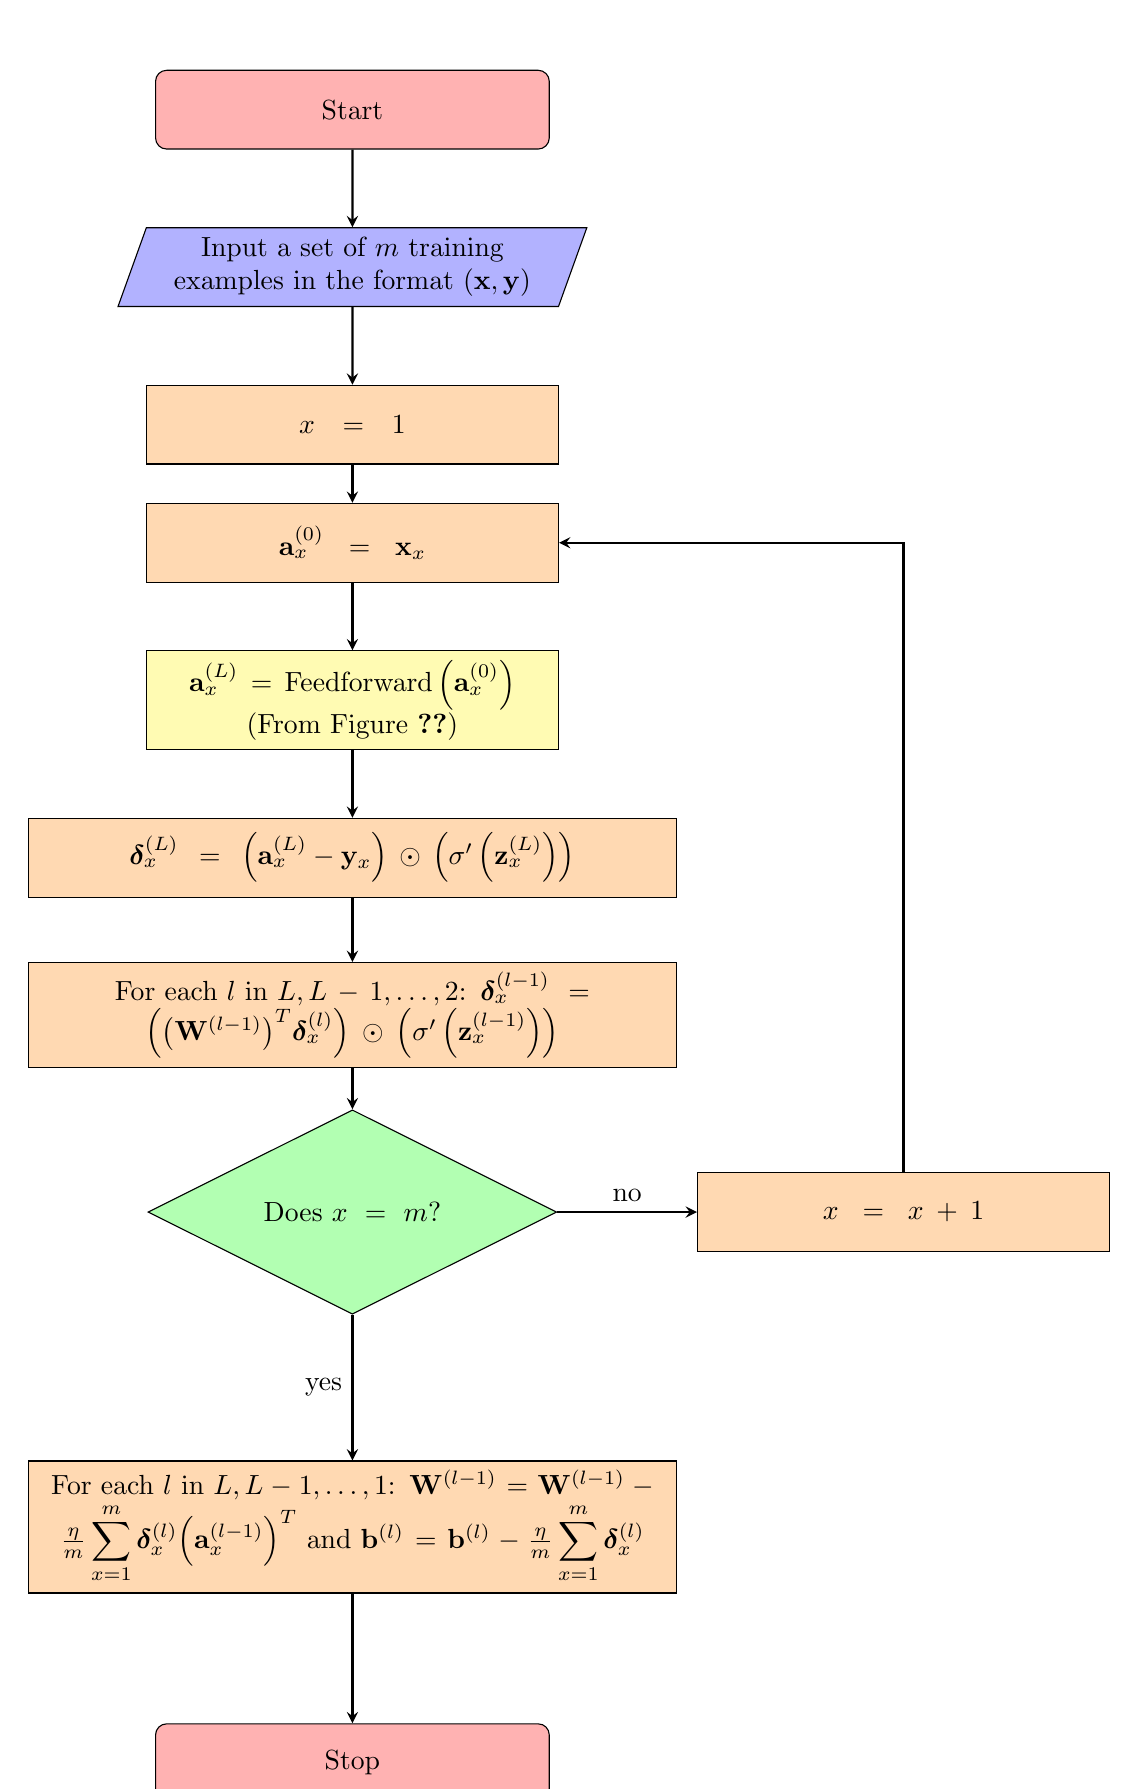
\begin{tikzpicture}[node distance=2cm]
    \node (start) [fStartStop] {Start};
    \node (intrainingexamples) [fInputOutput, below of=start] {Input a set of $m$ training examples in the format $\left(\mathbf{x},\mathbf{y}\right)$};
    \node (xequals1) [fProcess, below of=intrainingexamples] {$x=1$};
    \node (a0equalsx) [fProcess, below of=xequals1, yshift=0.5cm] {$\mathbf{a}^{\left(0\right)}_x=\mathbf{x}_x$};
    \node (feedforward) [fSubprocess, below of=a0equalsx] {$\mathbf{a}^{\left(L\right)}_x=\text{Feedforward}\left(\mathbf{a}^{\left(0\right)}_x\right)$ (From Figure \ref{fig:feedforward})};
    \node (erroroutputlayer) [fProcess, below of=feedforward, text width=8cm] {$\bm{\delta}^{\left(L\right)}_x=\left(\mathbf{a}^{\left(L\right)}_x-\mathbf{y}_x\right)\odot \left({\sigma}^{\prime} \left(\mathbf{z}^{\left(L\right)}_x\right)\right)$};
    \node (backpropogate) [fProcess, below of=erroroutputlayer, text width=8cm] {For each $l$ in $L,L-1,\ldots,2$: $\bm{\delta}^{\left(l-1\right)}_x=\left({\left(\mathbf{W}^{\left(l-1\right)}\right)}^{T}\bm{\delta}^{\left(l\right)}_x\right)\odot\left({\sigma}^{\prime} \left(\mathbf{z}^{\left(l-1\right)}_x\right)\right)$};
    \node (decisionx) [fDecision, below of=backpropogate, yshift=-0.5cm] {Does $x=m$?};
    \node (incrementx) [fProcess, right of=decisionx, xshift=5cm] {$x=x+1$};
    \node (gradientdescent) [fProcess, below of=decisionx, yshift=-2cm, text width=8cm] {For each $l$ in $L,L-1,\ldots,1$: $\mathbf{W}^{\left(l-1\right)}=\mathbf{W}^{\left(l-1\right)}-\frac{\eta}{m}\displaystyle\sum_{x=1}^{m}\bm{\delta}^{\left(l\right)}_x{\left(\mathbf{a}^{\left(l-1\right)}_x\right)}^T$ and $\mathbf{b}^{\left(l\right)}=\mathbf{b}^{\left(l\right)}-\frac{\eta}{m}\displaystyle\sum_{x=1}^{m}\bm{\delta}^{\left(l\right)}_x$};
    \node (stop) [fStartStop, below of=gradientdescent, yshift=-1cm] {Stop};
    
    \draw [fArrow] (start) -- (intrainingexamples);
    \draw [fArrow] (intrainingexamples) -- (xequals1);
    \draw [fArrow] (xequals1) -- (a0equalsx);
    \draw [fArrow] (a0equalsx) -- (feedforward);
    \draw [fArrow] (feedforward) -- (erroroutputlayer);
    \draw [fArrow] (erroroutputlayer) -- (backpropogate);
    \draw [fArrow] (backpropogate) -- (decisionx);
    \draw [fArrow] (decisionx) -- node[anchor=east] {yes} (gradientdescent);
    \draw [fArrow] (decisionx) -- node[anchor=south] {no} (incrementx);
    \draw [fArrow] (incrementx) |- (a0equalsx);
    \draw [fArrow] (gradientdescent) -- (stop);
\end{tikzpicture}
\caption{Backpropogation Algorithm Flowchart}\label{fig:backpropogation}
\end{figure}

\subsection{Stochastic Gradient Descent}\label{sec:sgd}
In practice, averaging over all the training examples is not very efficient, as you have to create a copy of the column vectors $\mathbf{a}$, $\mathbf{z}$ and $\bm{\delta}$ for each layer and training example, which can get very large very fast.

To combat this, instead break up the training data into mini batches which are easier to handle, while still having enough to represent a range of things that the network may want to look for. The training examples are also randomly shuffled before being sorted into mini batches to ensure that the contents of each one are different every time.

\begin{figure}[H]
\centering
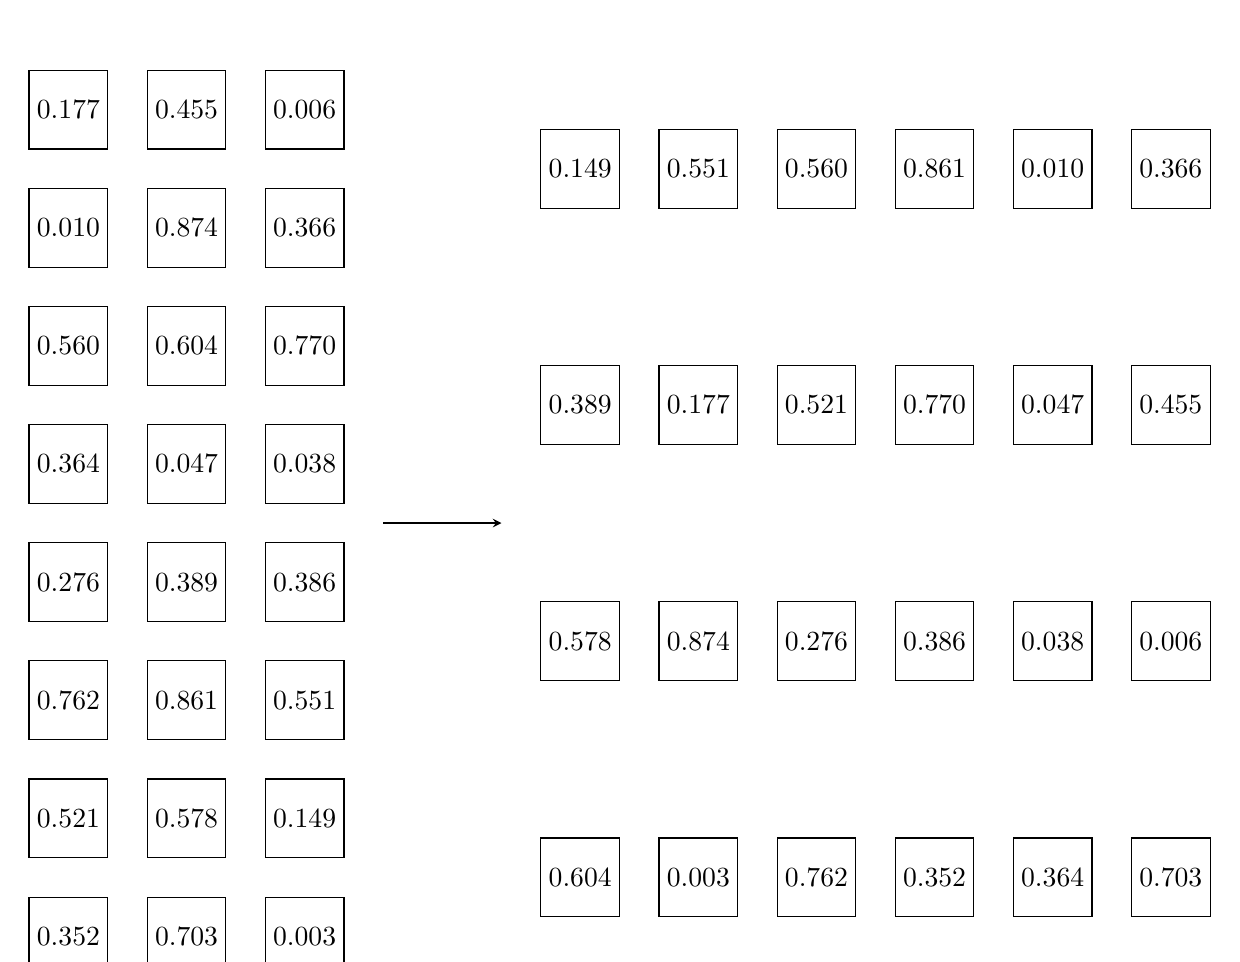
\begin{tikzpicture}
    \draw (0,0) rectangle (1,1) node[pos=.5] {0.352};
    \draw (1.5,0) rectangle (2.5,1) node[pos=.5] {0.703};
    \draw (3,0) rectangle (4,1) node[pos=.5] {0.003};
    \draw (0,1.5) rectangle (1,2.5) node[pos=.5] {0.521};
    \draw (1.5,1.5) rectangle (2.5,2.5) node[pos=.5] {0.578};
    \draw (3,1.5) rectangle (4,2.5) node[pos=.5] {0.149};
    \draw (0,3) rectangle (1,4) node[pos=.5] {0.762};
    \draw (1.5,3) rectangle (2.5,4) node[pos=.5] {0.861};
    \draw (3,3) rectangle (4,4) node[pos=.5] {0.551};
    \draw (0,4.5) rectangle (1,5.5) node[pos=.5] {0.276};
    \draw (1.5,4.5) rectangle (2.5,5.5) node[pos=.5] {0.389};
    \draw (3,4.5) rectangle (4,5.5) node[pos=.5] {0.386};
    \draw (0,6) rectangle (1,7) node[pos=.5] {0.364};
    \draw (1.5,6) rectangle (2.5,7) node[pos=.5] {0.047};
    \draw (3,6) rectangle (4,7) node[pos=.5] {0.038};
    \draw (0,7.5) rectangle (1,8.5) node[pos=.5] {0.560};
    \draw (1.5,7.5) rectangle (2.5,8.5) node[pos=.5] {0.604};
    \draw (3,7.5) rectangle (4,8.5) node[pos=.5] {0.770};
    \draw (0,9) rectangle (1,10) node[pos=.5] {0.010};
    \draw (1.5,9) rectangle (2.5,10) node[pos=.5] {0.874};
    \draw (3,9) rectangle (4,10) node[pos=.5] {0.366};
    \draw (0,10.5) rectangle (1,11.5) node[pos=.5] {0.177};
    \draw (1.5,10.5) rectangle (2.5,11.5) node[pos=.5] {0.455};
    \draw (3,10.5) rectangle (4,11.5) node[pos=.5] {0.006};
    \draw[-stealth] (4.5,5.75) -- (6,5.75);
    \draw (6.5,0.75) rectangle (7.5,1.75) node[pos=0.5] {0.604};
    \draw (8,0.75) rectangle (9,1.75) node[pos=0.5] {0.003};
    \draw (9.5,0.75) rectangle (10.5,1.75) node[pos=0.5] {0.762};
    \draw (11,0.75) rectangle (12,1.75) node[pos=0.5] {0.352};
    \draw (12.5,0.75) rectangle (13.5,1.75) node[pos=0.5] {0.364};
    \draw (14,0.75) rectangle (15,1.75) node[pos=0.5] {0.703};
    \draw (6.5,3.75) rectangle (7.5,4.75) node[pos=0.5] {0.578};
    \draw (8,3.75) rectangle (9,4.75) node[pos=0.5] {0.874};
    \draw (9.5,3.75) rectangle (10.5,4.75) node[pos=0.5] {0.276};
    \draw (11,3.75) rectangle (12,4.75) node[pos=0.5] {0.386};
    \draw (12.5,3.75) rectangle (13.5,4.75) node[pos=0.5] {0.038};
    \draw (14,3.75) rectangle (15,4.75) node[pos=0.5] {0.006};
    \draw (6.5,6.75) rectangle (7.5,7.75) node[pos=0.5] {0.389};
    \draw (8,6.75) rectangle (9,7.75) node[pos=0.5] {0.177};
    \draw (9.5,6.75) rectangle (10.5,7.75) node[pos=0.5] {0.521};
    \draw (11,6.75) rectangle (12,7.75) node[pos=0.5] {0.770};
    \draw (12.5,6.75) rectangle (13.5,7.75) node[pos=0.5] {0.047};
    \draw (14,6.75) rectangle (15,7.75) node[pos=0.5] {0.455};
    \draw (6.5,9.75) rectangle (7.5,10.75) node[pos=0.5] {0.149};
    \draw (8,9.75) rectangle (9,10.75) node[pos=0.5] {0.551};
    \draw (9.5,9.75) rectangle (10.5,10.75) node[pos=0.5] {0.560};
    \draw (11,9.75) rectangle (12,10.75) node[pos=0.5] {0.861};
    \draw (12.5,9.75) rectangle (13.5,10.75) node[pos=0.5] {0.010};
    \draw (14,9.75) rectangle (15,10.75) node[pos=0.5] {0.366};
\end{tikzpicture}
\caption{Shuffling into Mini Batches}
\end{figure}

When carrying out the gradient descent, this will have the effect of taking a step in some direction close to that which decreases the gradient by the most, instead of going directly in that direction. This is called Stochastic Gradient Descent.

Finally, this entire process should be repeated multiple times, over a number of ``epochs'', in order to ensure that it has enough time to learn.

\begin{figure}[H]
\centering
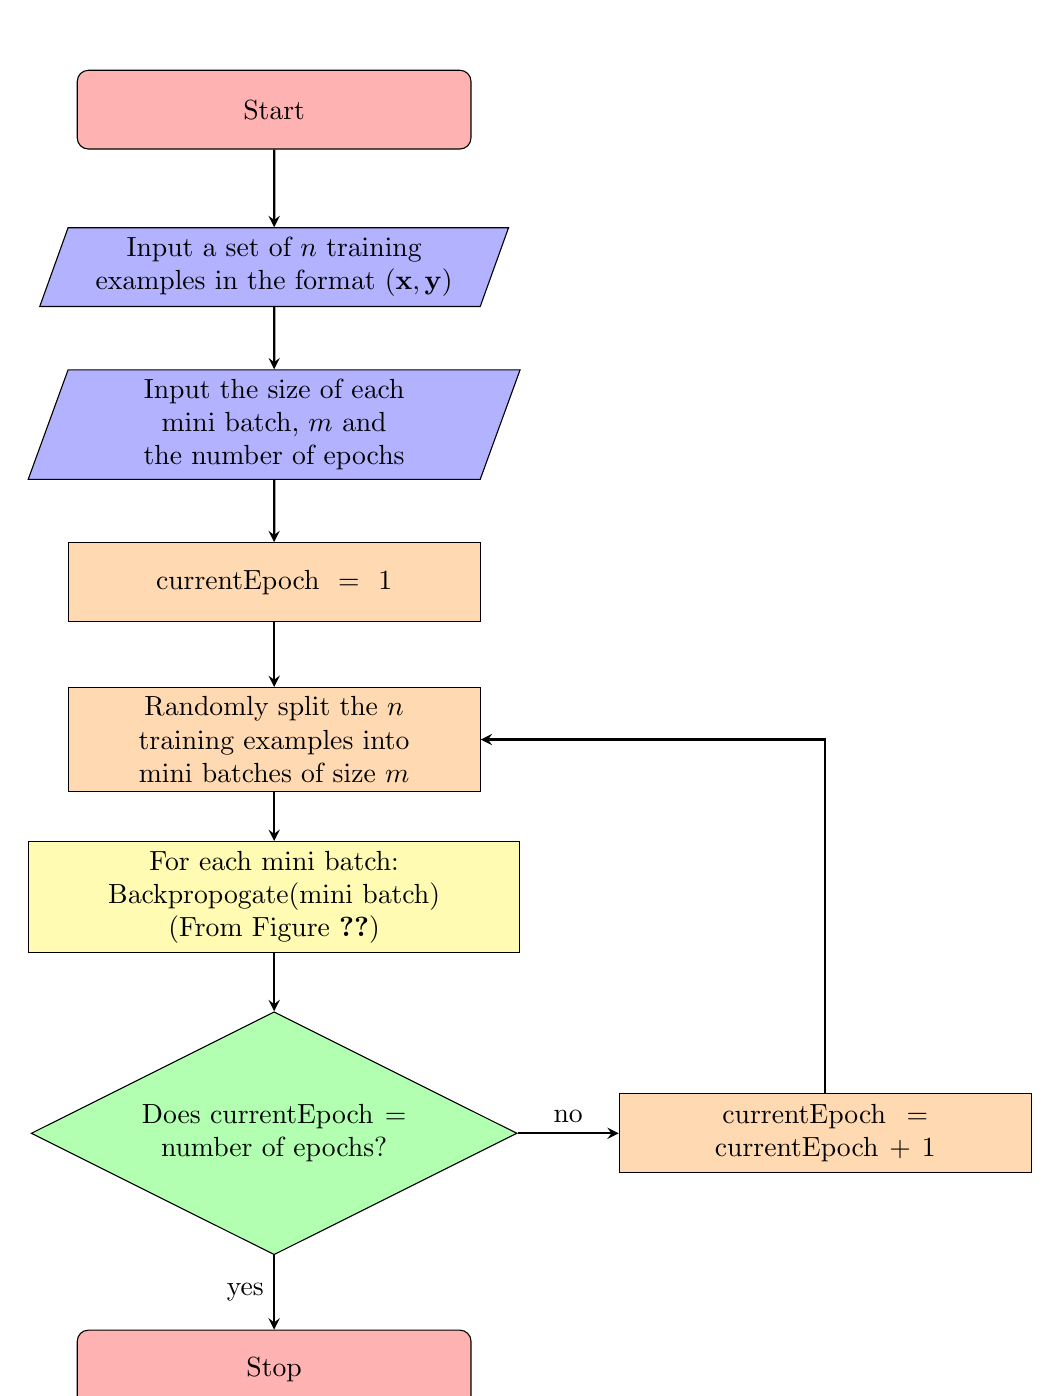
\begin{tikzpicture}[node distance=2cm]
    \node (start) [fStartStop] {Start};
    \node (inexamples) [fInputOutput, below of=start] {Input a set of $n$ training examples in the format $\left(\mathbf{x},\mathbf{y}\right)$};
    \node (inconsts) [fInputOutput, below of=inexamples] {Input the size of each mini batch, $m$ and the number of epochs};
    \node (epoch1) [fProcess, below of=inconsts] {$\text{currentEpoch}=1$};
    \node (minibatches) [fProcess, below of=epoch1] {Randomly split the $n$ training examples into mini batches of size $m$};
    \node (backpropogate) [fSubprocess, below of=minibatches, text width=6cm] {For each mini batch:\\Backpropogate(mini batch)\\(From Figure \ref{fig:backpropogation})};
    \node (decision) [fDecision, below of=backpropogate, yshift=-1cm] {Does $\text{currentEpoch}=\text{number of epochs}$?};
    \node (incrementepoch) [fProcess, right of=decision, xshift=5cm] {$\text{currentEpoch}=\text{currentEpoch}+1$};
    \node (stop) [fStartStop, below of=decision, yshift=-1cm] {Stop};
    
    \draw [fArrow] (start) -- (inexamples);
    \draw [fArrow] (inexamples) -- (inconsts);
    \draw [fArrow] (inconsts) -- (epoch1);
    \draw [fArrow] (epoch1) -- (minibatches);
    \draw [fArrow] (minibatches) -- (backpropogate);
    \draw [fArrow] (backpropogate) -- (decision);
    \draw [fArrow] (decision) -- node[anchor=east] {yes} (stop);
    \draw [fArrow] (decision) -- node[anchor=south] {no} (incrementepoch);
    \draw [fArrow] (incrementepoch) |- (minibatches);
\end{tikzpicture}
\caption{Full Training Algorithm Flowchart}
\end{figure}

\subsection{Class Diagram}
\begin{figure}[H]
\centering
\begin{tabular}{| m{15cm} |} 
    \hline
    \pil{class MultilayerPerceptron(object)} \\
    \hline
    \pil{layer_sizes: list[int]} \\
    \pil{L: int} \\
    \pil{activations: list[column_vector]} \\
    \pil{weights: list[matrix]} \\
    \pil{biases: list[column_vector]} \\
    \pil{z: list[column_vector]} \\
    \pil{errors: list[column_vector]} \\
    \pil{training_activations: list[list[column_vector]]} \\
    \pil{training_z: list[list[column_vector]]} \\
    \pil{training_errors: list[list[column_vector]]} \\
    \hline
    \pil{def __init__(self, layer_sizes)} \\
    \pil{def predict(self, input_data)} \\
    \pil{def train(self, examples, mini_batch_size, num_epochs, learning_rate)} \\
    \pil{def feedforward(self, a0)} \\
    \pil{def backpropogate(self, examples)} \\
    \pil{def sigmoid(self, x)} \\
    \pil{def sigmoid_prime(self, x)} \\
    \pil{def save_model(self, filename)} \\
    \pil{def load_model(self, file_path)} \\
    \hline
\end{tabular}
\caption{Multilayer Perceptron Class Diagram}\label{fig:classDiagram}
\end{figure}

The attribute \pil{layer_sizes} is a list of integers, which represent the number of neurons in each layer. The attributes \pil{L} and \pil{z} represent the respective variables in the mathematical explanation above, \pil{activations} represents the $\mathbf{a}$ vectors, \pil{weights} represents the $\mathbf{W}$ matrices, \pil{biases} represents the $\mathbf{b}$ vectors, and \pil{errors} represents the $\bm{\delta}$ vectors. The data structures \pil{column_vector} and \pil{matrix} are not built into python, but come with the library \pil{numpy}. The attributes \pil{training_activations}, \pil{training_z} and \pil{training_errors} will hold the values for each of the training examples in a mini batch, as all of them need to be computed for each example before the gradient is calculated (which is why they are in an extra \pil{list}).

The constructor method (\pil{def __init__}) only takes in the layer sizes, as everything else will either be defined during training or prediction, or be initially set to random values. The other methods are as you would expect, with functions for prediction and training that are explained above. There are also the methods \pil{def save_model} and \pil{def load_model}, as the model will be trained beforehand and then the GUI will query that model. Therefore, we need a way of saving the weights and biases to an external file and then loading them from it at a later time.

All the methods will be public functions, as python does not allow for anything else. However, in theory, they would all be procedures except for \pil{def predict}, \pil{def sigmoid} and \pil{def sigmoid_prime}, which will all return \pil{float}s, while the rest will return \pil{None}.

There is not a ``List of key variables'' for this section, as all the results of calculations will be stored in the attributes in the \pil{class MultilayerPerceptron}, and have therefore been described above.

\section{User Interface}\label{sec:ui}
There are many features I would like to add eventually, which I have included in the Structure Diagram (Figure \ref{fig:structDiagram}). I will not be including these in this section, and will be saving them for the next prototype. I will only be planning for the user entering their region on a map, the HDI being predicted, and the suggestions for improvements being made, as I believe these are the most essential feautures.
\subsection{Interface Sketch}
\begin{figure}[H]
\centering
\begin{tikzpicture}
    % border
    \draw (0,0) rectangle (15,12);
    % map
    \path[fill stretch image=map] (0.5,11.5) rectangle (9,6);
    \draw (0.5,11.5) rectangle (9,6);
    \draw[fill=white] (0.5,11.5) rectangle (1,11);
    \draw (0.65,11.1) -- (0.588196601125,11.290211303259) -- (0.75,11.4077683537175) -- (0.911803398875,11.290211303259) -- (0.85,11.1) -- cycle;
    \draw[fill=white] (0.5,10.75) rectangle (1,10.25);
    \draw (0.6,10.5) -- (0.9,10.5);
    \draw (0.75,10.65) -- (0.75,10.35);
    \draw[fill=white] (0.5,10.25) rectangle (1,9.75);
    \draw (0.6,10) -- (0.9,10);
    \draw[fill=white] (0.5,9.5) rectangle (1,9);
    \draw (0.6,9.4) -- (0.9,9.1);
    \draw (0.6,9.1) -- (0.9,9.4);
    \draw[blue,fill=blue!80,fill opacity=0.4] (1.65,9.25) rectangle (3,8.5);
    \filldraw[red] (2.3,8.9) circle (0.05); 
    %predict button section
    \draw[fill=orange] (9.5,11.5) rectangle (14.5,10.5) node[pos=0.5] {Predict};
    \draw (9.5,10) node[anchor=north west] {{\scriptsize I believe the HDI of this area is...}};
    \draw (9.5,10) rectangle (14.5,8.5) node[pos=0.5] {0.927};
    \draw (9.5,8) node[anchor=north west] {{\scriptsize That's a similar HDI to...}};
    \draw (9.5,8) rectangle (14.5,6) node[pos=0.5] {The USA};
    %suggestions
    \draw (0.5,4.5) node[anchor=south west] {{\scriptsize New Building}};
    \draw (3,4.5) node[anchor=south west] {{\scriptsize Coordinates}};
    \draw (9,4.5) node[anchor=south west] {{\scriptsize New HDI}};
    \draw (11.5,4.5) node[anchor=south west] {{\scriptsize Change in HDI}};
    \draw (0.5,4.5) rectangle (3,4) node[pos=0.5] {School};
    \draw (3,4.5) rectangle (9,4) node[pos=0.5] {$36.922883^{\circ}\text{N},-101.709461^{\circ}\text{E}$};
    \draw (9,4.5) rectangle (11.5,4) node[pos=0.5] {0.928};
    \draw (11.5,4.5) rectangle (14.5,4) node[pos=0.5] {$+0.001$};
    \draw[fill=cyan!20] (0.5,4) rectangle (3,3.5) node[pos=0.5] {Hospital};
    \draw[fill=cyan!20] (3,4) rectangle (9,3.5) node[pos=0.5] {$43.919052^{\circ}\text{N},-106.264212^{\circ}\text{E}$};
    \draw[fill=cyan!20] (9,4) rectangle (11.5,3.5) node[pos=0.5] {0.929};
    \draw[fill=cyan!20] (11.5,4) rectangle (14.5,3.5) node[pos=0.5] {$+0.002$};
    \draw (0.5,3.5) rectangle (3,3) node[pos=0.5] {Library};
    \draw (3,3.5) rectangle (9,3) node[pos=0.5] {$36.954162^{\circ}\text{N},-87.008695^{\circ}\text{E}$};
    \draw (9,3.5) rectangle (11.5,3) node[pos=0.5] {0.928};
    \draw (11.5,3.5) rectangle (14.5,3) node[pos=0.5] {$+0.001$};
    \draw (7.5,2.5) node {$\vdots$};
    % note
    \draw (0,0) node[anchor=south west] {{\scriptsize (The data presented in this sketch is completely made up but somewhat realistic)}};
    % annotations
    \draw[red,->] (7.5,12.5) node[red,above] {1.} -- (7.5,11.5);
    \draw[red,->] (0.75,12.5) node[red,above] {2.} -- (0.75,11.5);
    \draw[red,->] (-0.5,10.25) node[red,left] {3.} -- (0.5,10.25);
    \draw[red,->] (-0.5,9.25) node[red,left] {4.} -- (0.5,9.25);
    \draw[red,->] (-0.5,8.875) node[red,left] {5.} -- (1.65,8.875);
    \draw[red,->] (15.5,11) node[red,right] {6.} -- (14.5,11);
    \draw[red,->] (15.5,9.25) node[red,right] {7.} -- (14.5,9.25);
    \draw[red,->] (15.5,7) node[red,right] {8.} -- (14.5,7);
    \draw[red,->] (-0.5,5) node[red,left] {9.} -- (0.25,4.75);
    \draw[red,->] (-0.5,3.75) node[red,left] {10.} -- (0.5,3.75);
    \draw[red,->] (3,8.2) node[red,below right] {11.} -- (2.4,8.8);
\end{tikzpicture}
\caption{Technical Interface Sketch}\label{fig:interfaceSketch1}
\end{figure}

The labelled items shown in Figure \ref{fig:interfaceSketch1} are:
\begin{enumerate}
    \item Map for the user to draw on
    \item Button to toggle between using the mouse for polygon drawing and moving
    \item Zoom in and out buttons
    \item Cancel Button
    \item Example area the user may draw
    \item Predict Button
    \item Predicted HDI
    \item A comparison to a country with a similar HDI
    \item A list of suggestions to improve the HDI
    \item A selected suggestion to view in more detail (that the user has selected)
    \item The location on the map for the selected suggestion
\end{enumerate}

Figure \ref{fig:interfaceSketch1} shows the general structure of the user interface, while the style will be provided by the \pil{gradio} python module. Exampled of the style can be seen in Figure \ref{fig:interfaceStyle}. It will automatically adapt to light mode or dark mode based on the device's or browser's settings.
\begin{figure}[H]
\centering
\begin{subfigure}{.8\textwidth}
    \centering
    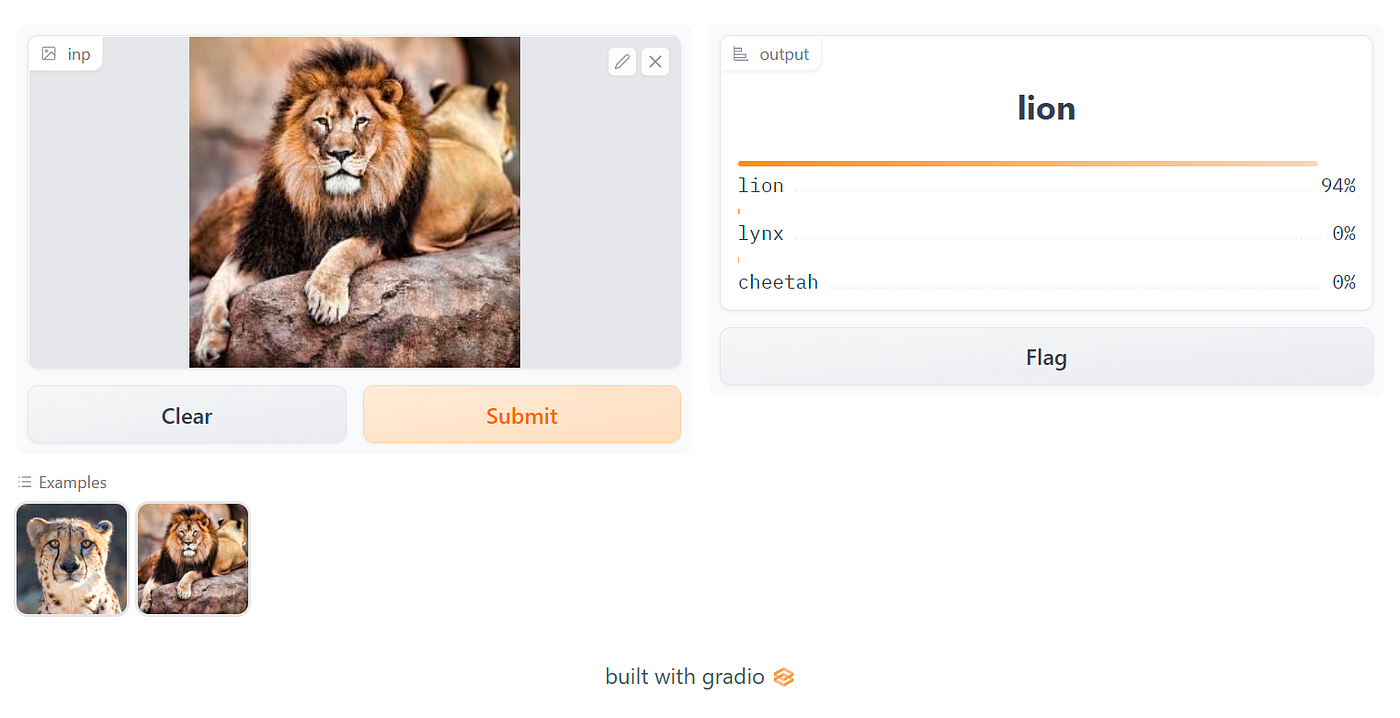
\includegraphics[width=.9\linewidth]{lightModeInterface.png}
    \caption{Light Mode}
\end{subfigure}
\begin{subfigure}{.8\textwidth}
    \centering
    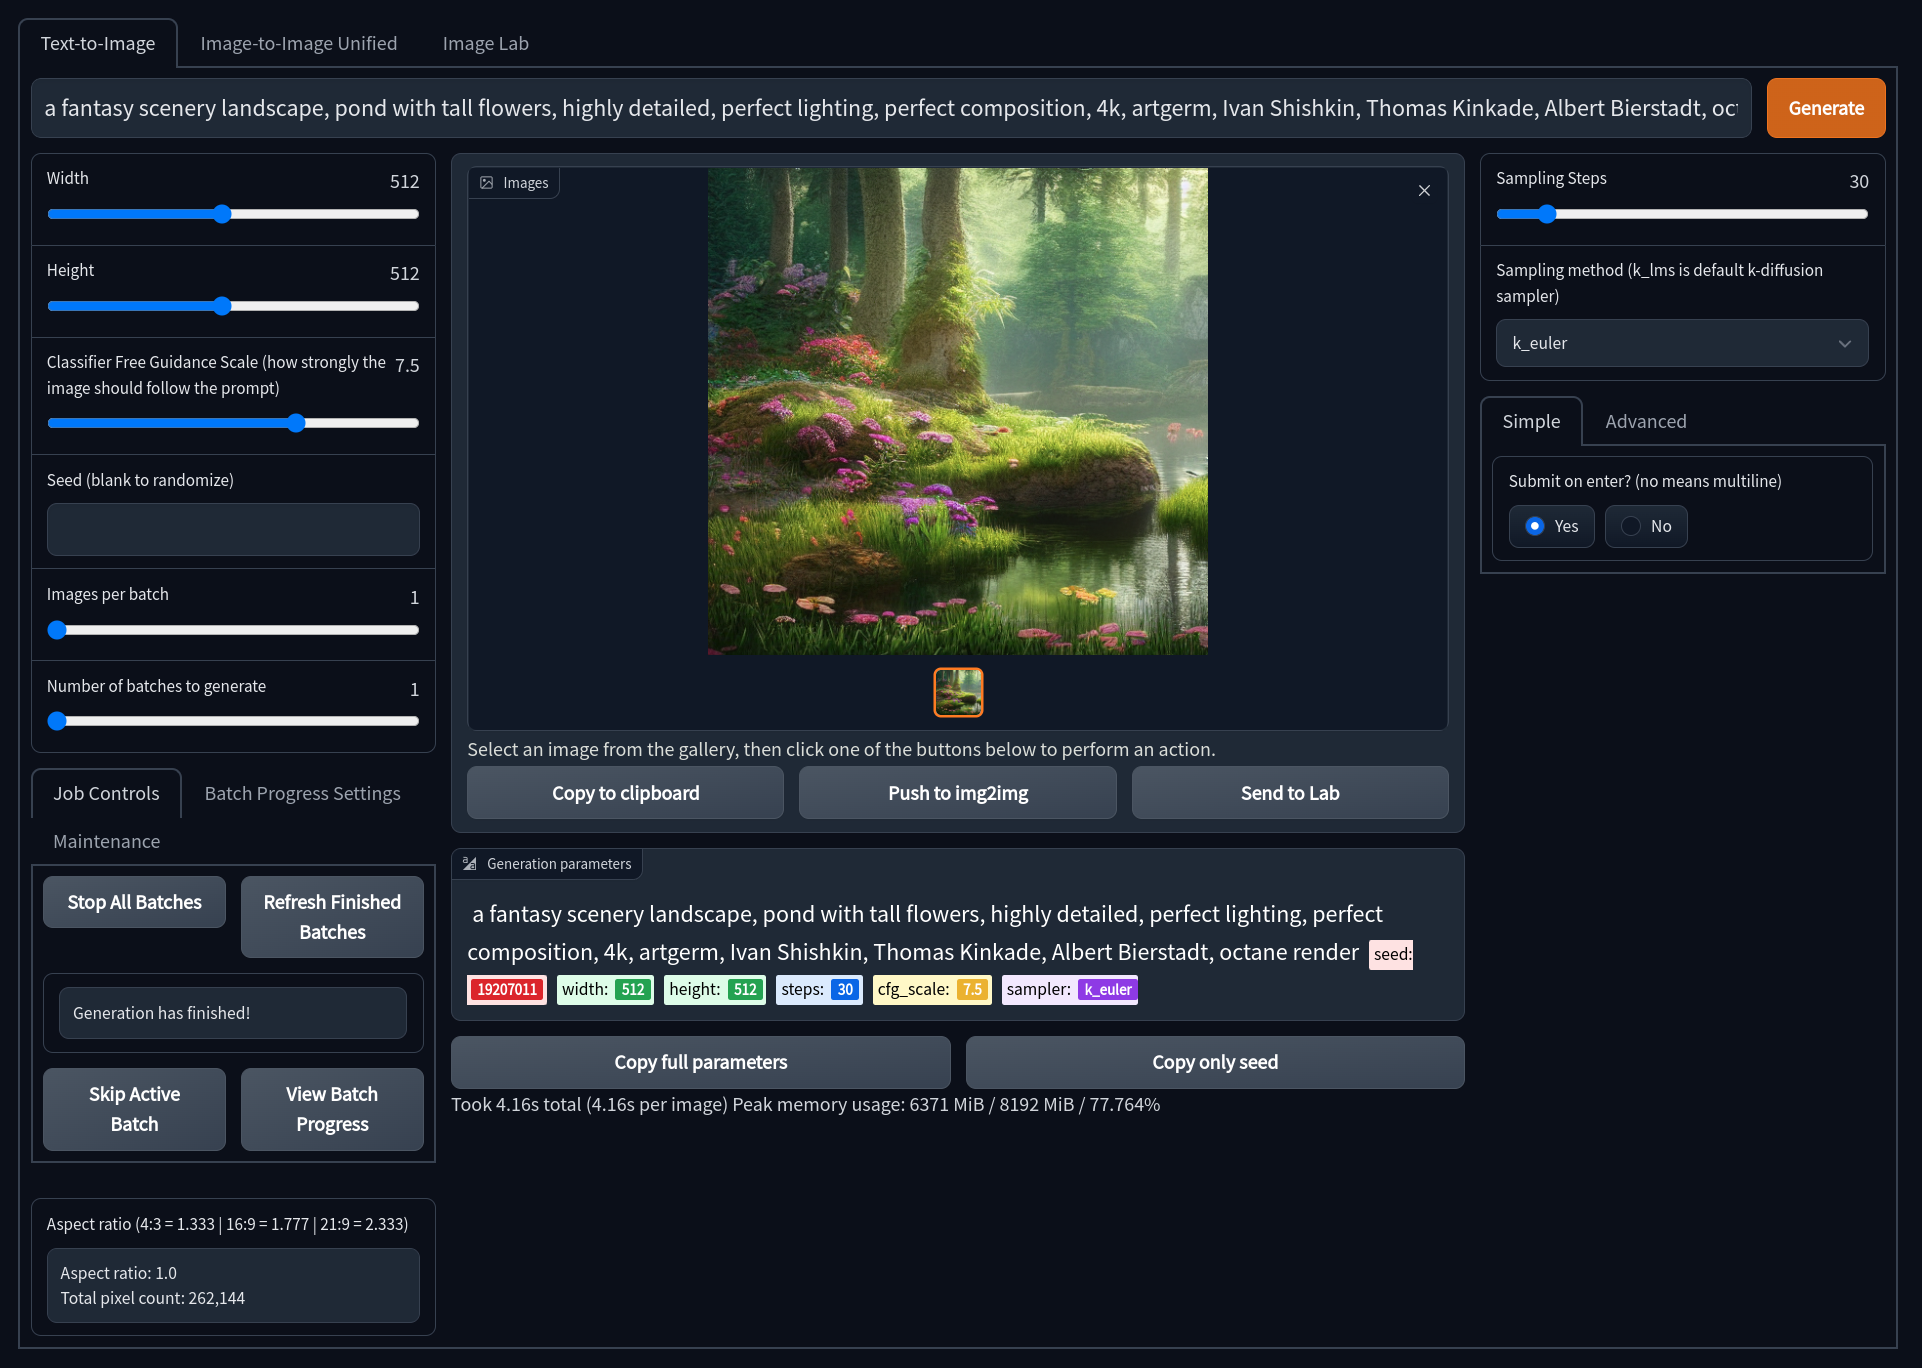
\includegraphics[width=.9\linewidth]{darkModeInterface.png}
    \caption{Dark Mode}
\end{subfigure}
\caption{Interface Style Examples}\label{fig:interfaceStyle}
\end{figure}

Additional features that will be added in later prototypes (such as an analysis of how much each factor affects the others or entering factors manually) will be accessed from different tabs at the top of the interface.

\subsection{Input Validation}
As the only input the user is providing is that of drawing on the map to select their region (for now), only that needs to be validated. I will ensure that the user can only draw polygons on the map, the polygons must be completed, and the polygons cannot self intersect. The mapping module I will be using, \pil{folium} already accounts for this, except for the self intersection. However, this can be detected by using part of the $D\left(x\right)$ algorithm, as shown in Figure \ref{fig:dofx}.

The user should also only be able to interact with the map and any data visualisations. The GUI module I will be using, \pil{gradio} also already accounts for this.

\subsection{Usability Features}
\subsubsection{Map \& Map Buttons}
The map should be the biggest thing on the screen, as it is the main source of input the user will be providing. It should also be as big as possible to accomodate those with smaller screens, so that they can still accurately pinpoint locations.

The button to draw a polygon on the map will be displayed as a regular pentagon. This is because there are often distinct tools to draw rectangles or triangles, which would be represented by regular 4-sided or 3-sided polygons respectively. Therefore, if a regular 5-sided polygon is used (a pentagon) there is less likely to be confusion about what the button does, while still having a small number of sides (a large number of sides will look too similar to a circle). It also suggests that the user will not be able to draw freely (as this is often represented by a pencil), which they will not be able to do.

The buttons to zoom in and out will be represented by a plus and minus sign. This is also the standard design for this type of button. The zoom in button and zoom out buttons will be right next to each other, to minimise the consequence in accidentally zooming in/out one too many times.

The button to cancel will be represented by an X, as this is also a common symbol used for this type of button. It will be in the same approximate location as the other 3 buttons, as they all have similar functions.

The region the user draws will be shown in blue, and filled with a slightly transparent blue. This is so that they can see the region that they are drawing in real time, while also still being able to see the map beneath it.

\subsubsection{Prediction of HDI}
The button to make the prediction (and submit the region they have drawn) will be the largest button on the screen, and in the primary colour. By default, the primary colour of \pil{gradio} interfaces is orange, as it compliments the (default, dark mode) dark blue background. This will make it very easy for the user to see what they need to do.

The 2 pieces of information below the predict button (the predicted HDI and the country comparison) will have the largest text size out of all the elements in the interface. This is because this is most likely the main information the user is trying to find, and so should be easy to find. Placing these elements next to the predict button is for the same reason.

\subsubsection{Suggestions to Improve HDI}
The suggestions to improve the HDI will be given in a table, as they will all follow a similar format: \textit{``Build a new (building) at (these coordinates) to improve the HDI by (this much), which increases it to (this value).''}. This information can be efficiently organised into a table, in order to retrieve the most important information quickly.

Each row of the table (each suggestion) may be selected to show the location of that new building on the map. This is because reading coordinates such as $36.922883^{\circ}\text{N},-101.709461^{\circ}\text{E}$ does not give an intiutive sense of location, especially within a small area.

\subsection{Finding an Optimal Place for a New Building}\label{sec:optimalPlace}
When suggestions are being made to the user to improve the HDI, they will be in the format: ``Build a new \textit{some building} at \textit{some coordinates}''. Which building will be determined from a predefined list of possible suggestions, which will match the factors I am considering. The coordinates at which to place it are harder to determine.

In theory, increasing the Density factor involving this building, and decreasing the Average Distance factors involving this building will increase the HDI. No matter where we place the new building in the region, the Density factor will increase by the same amount, as the number of that building will always increase by 1, and the area of the region will never change.

Therefore, we only need to consider how the position of a new building will affect the Average Distance factors. Any place we choose will decrease it by some amount, but we need to find a place that will decrease it by a significant amount. Finding the \textit{exact} optimal place is very difficult, so instead I will be using a heuristic, ``good enough'' approach.

One way that I would consider is ``good enough'', is finding the midpoint of all the positions of the other objects, to find where to place this new building. For example, if we wish to decrease $A\left(\text{House},\text{Hospital}\right)$, we could place a hospital in the midpoint of all the positions of the houses. This will involve taking a mean of all the latitude and longitude coordinates of all the houses.

However, there may be some other factors involving hospitals, such as $A\left(\text{School},\text{Hospital}\right)$ for which we would need to follow the same procedure. This will result in a different optimal place to what was calculated from the houses.

To make a compromise between all the factors that involve the building we are trying to place, we can average the previously calculated optimal places for each different factor to get an overall optimal place to build the building.
\begin{figure}[H]
\centering
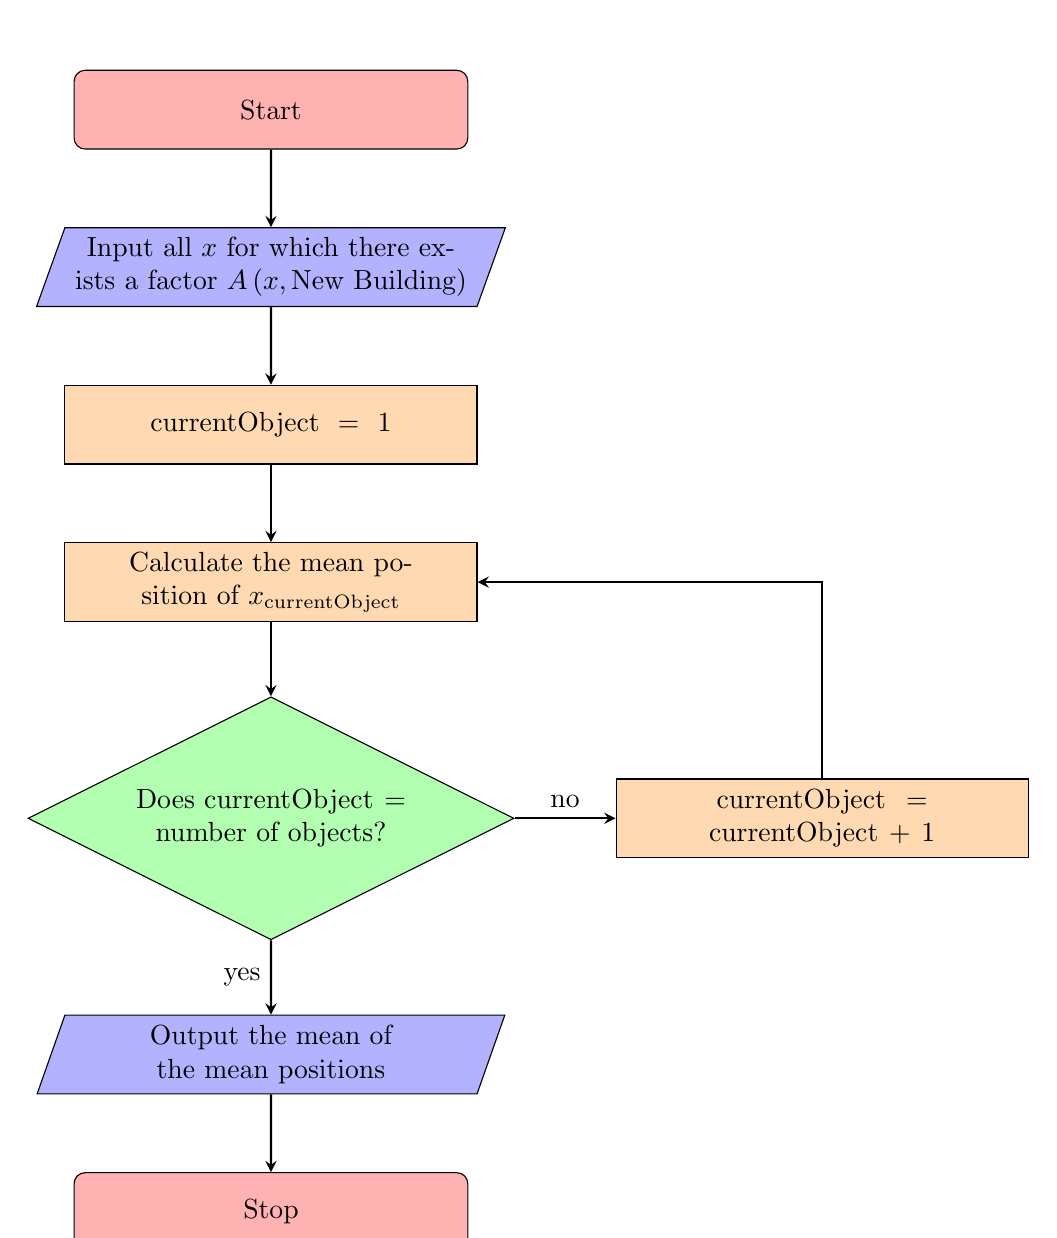
\begin{tikzpicture}[node distance=2cm]
    \node (start) [fStartStop] {Start};
    \node (in) [fInputOutput, below of=start] {Input all $x$ for which there exists a factor $A\left(x,\text{New Building}\right)$};
    \node (object1) [fProcess, below of=in] {$\text{currentObject}=1$};
    \node (meanPos) [fProcess, below of=object1] {Calculate the mean position of $x_{\text{currentObject}}$};
    \node (decision) [fDecision, below of=meanPos, yshift=-1cm] {Does $\text{currentObject}=\text{number of objects}$?};
    \node (incrementobject) [fProcess, right of=decision, xshift=5cm] {$\text{currentObject}=\text{currentObject}+1$};
    \node (out) [fInputOutput, below of=decision, yshift=-1cm] {Output the mean of the mean positions};
    \node (stop) [fStartStop, below of=out] {Stop};
    
    \draw [fArrow] (start) -- (in);
    \draw [fArrow] (in) -- (object1);
    \draw [fArrow] (object1) -- (meanPos);
    \draw [fArrow] (meanPos) -- (decision);
    \draw [fArrow] (decision) -- node[anchor=east] {yes} (out);
    \draw [fArrow] (decision) -- node[anchor=south] {no} (incrementobject);
    \draw [fArrow] (incrementobject) |- (meanPos);
    \draw [fArrow] (out) -- (stop);
\end{tikzpicture}
\caption{Finding an Optimal Place for New Building Flowchart}\label{fig:newBuilding}
\end{figure}
For validation, this function should only be called when there exists at least 1 factor in the form $A\left(x,\text{New Building}\right)$.

I intend to implement a better algorithm to find an optimal place for a new building in future prototypes, however this will do for now.

\subsection{Overall Algorithm for User Predicting HDI}\label{sec:predictHDIFullAlgo}
The user will draw their region on the map, from that the relevant data will be retrieved from OSM using Overpass Turbo, and then the Density and Average Distance factors will be calculated. This will be fed into the pre-trained neural network, which will predict the HDI.

On top of this, a series of suggestions will be made to improve the HDI. The full list of suggestions I would like to make are (in no partucular order):
\begin{multicols}{2}
\begin{enumerate}
    \item Building a new School
    \item Building a new Hospital
    \item Building a new Place of Worship
    \item Building a new Police Station
    \item Building a new Restaurant
    \item Building a new Slot Machine
    \item Building a new Library
    \item Building a new Pharmacy
\end{enumerate}
\end{multicols}
For each of the suggested buildings, the position at which to build it must be calculated, and then the factors must be calculated again before being fed into the pre-trained neural network.
\begin{figure}[H]
\centering
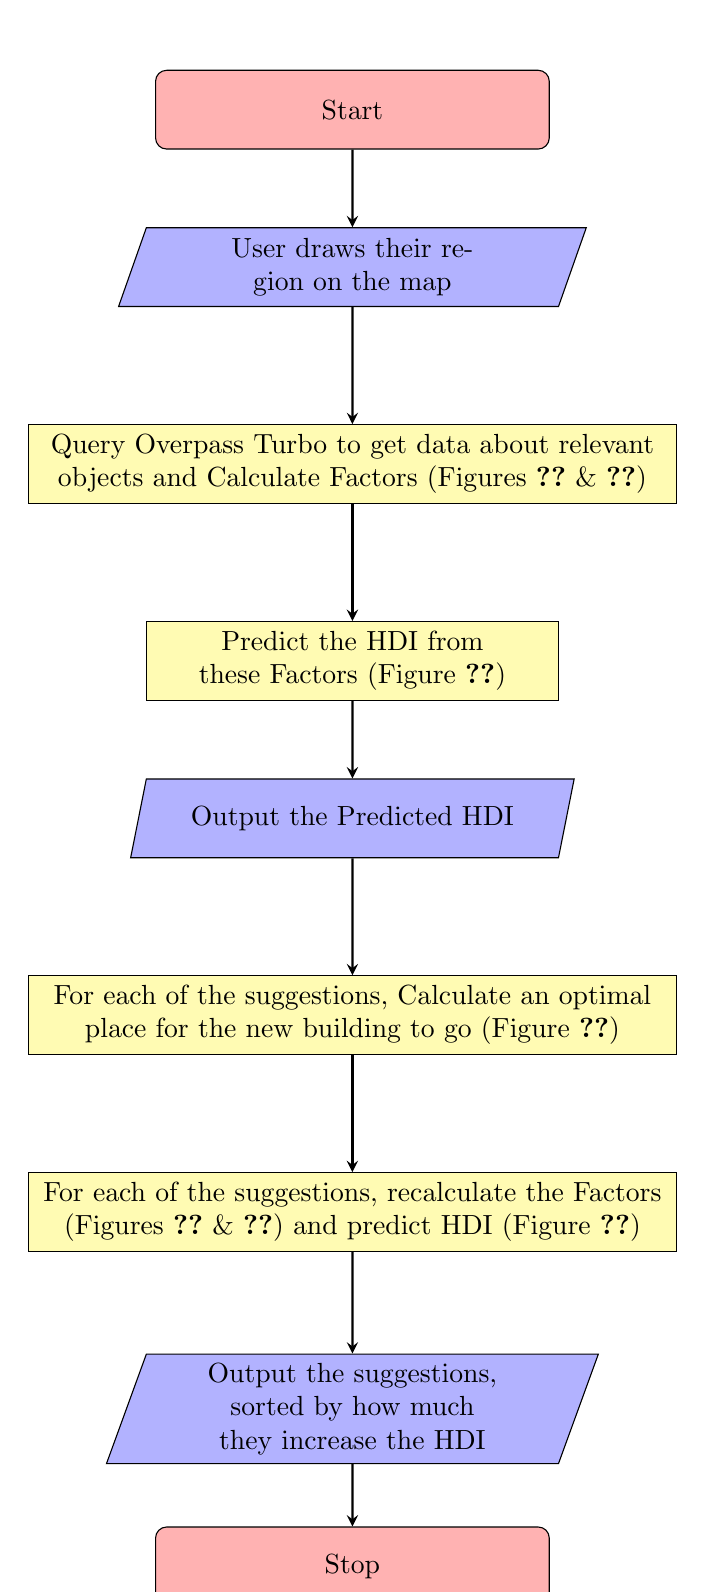
\begin{tikzpicture}[node distance=2cm]
    \node (start) [fStartStop] {Start};
    \node (drawMap) [fInputOutput, below of=start] {User draws their region on the map};
    \node (findFactors) [fSubprocess, below of=drawMap, text width=8cm, yshift=-0.5cm] {Query Overpass Turbo to get data about relevant objects and Calculate Factors (Figures \ref{fig:aofxy} \& \ref{fig:dofx})};
    \node (predictHDI) [fSubprocess, below of=findFactors, yshift=-0.5cm] {Predict the HDI from these Factors (Figure \ref{fig:feedforward})};
    \node (outHDI) [fInputOutput, below of=predictHDI] {Output the Predicted HDI};
    \node (calcPos) [fSubprocess, below of=outHDI, text width=8cm, yshift=-0.5cm] {For each of the suggestions, Calculate an optimal place for the new building to go (Figure \ref{fig:newBuilding})};
    \node (repredict) [fSubprocess, below of=calcPos, text width=8cm, yshift=-0.5cm] {For each of the suggestions, recalculate the Factors (Figures \ref{fig:aofxy} \& \ref{fig:dofx}) and predict HDI (Figure \ref{fig:feedforward})};
    \node (out) [fInputOutput, below of=repredict, yshift=-0.5cm] {Output the suggestions, sorted by how much they increase the HDI};
    \node (stop) [fStartStop, below of=out] {Stop};
    
    \draw [fArrow] (start) -- (drawMap);
    \draw [fArrow] (drawMap) -- (findFactors);
    \draw [fArrow] (findFactors) -- (predictHDI);
    \draw [fArrow] (predictHDI) -- (outHDI);
    \draw [fArrow] (outHDI) -- (calcPos);
    \draw [fArrow] (calcPos) -- (repredict);
    \draw [fArrow] (repredict) -- (out);
    \draw [fArrow] (out) -- (stop);
\end{tikzpicture}
\caption{Overall User Predicting HDI Algorithm Flowchart}
\end{figure}

\subsection{List of Key Variables}
\subsubsection{Variables in Finding Optimal Place for New Building}
\begin{center}
\begin{longtable}{ | m{3cm} | m{4cm}| m{4cm} | m{4cm} |} 
    \hline
    \textbf{Identifier} & \textbf{Data Type} & \textbf{Explanation}  & \textbf{Justification} \\ 
    \hline
    \pil{new_building_type} & \pil{str} & Holds the type of new building to be placed. & This is used to determine if there are any other factors which contain this type of building. \\ 
    \hline
    \pil{other_objects} & \pil{list[str]} & Holds each of the other types of object to consider. & We must iterate over this to find an optimal place for a new building. \\ 
    \hline
    \pil{current_object} & \pil{str} & Iterator variable for \pil{other_objects} & This will be used to keep track of which object we are currently considering \\ 
    \hline
    \pil{mean_positions} & \pil{list[tuple[float]]} & Holds the mean positions of all the other objects we are considering & This is a list of latitude and longitude coordinates, so a tuple is used as before. \\ 
    \hline
\caption{List of Key Variables in Finding Optimal Place for New Building}
\end{longtable}
\end{center}

\subsubsection{Other Variables}
\begin{center}
\begin{longtable}{ | m{3cm} | m{4cm}| m{4cm} | m{4cm} |} 
    \hline
    \textbf{Identifier} & \textbf{Data Type} & \textbf{Explanation}  & \textbf{Justification} \\ 
    \hline
    \pil{app} & \pil{object} & Contains the \pil{gradio} app, which will be ran on the local web server. & The app (highest level ``interface block'') must be stored in a variable to pass to the web server. \\ 
    \hline
    \pil{neural_network} & \pil{object} & Stores the pre-trained model for predicting HDI. & This must be called upon when the user draws their region on the map. \\ 
    \hline
    \pil{suggestions_types} & \pil{list[str]} & List containing the different types of suggestion to be made. & Each \pil{str} will be the name of the new building type to place. \\ 
    \hline
    \pil{suggestions} & \pil{dict[float]} & A dictionary, containing each predicted HDI, each with a key. & The key will be a string containing the type of new building. \\ 
    \hline
\caption{List of Other Key Variables in User Interface}
\end{longtable}
\end{center}

\section{Data}
\subsection{Data Structures}
\subsubsection{Coordinates}
Any time I am dealing with coordinates on the surface of the Earth, I will be using a \pil{tuple[float]}. The latitude and longitude are stored as \pil{float}s, as they are real numbers that may not be integers. They are stored in a \pil{tuple}, as the length of the data structure will never change (as that would correspond to adding a new perpendicular dimension), and the value of the coordinate never needs to be changed, and so \pil{tuple}s being immutable and static is suitable.

Coordinates in 3D space can also be stored as \pil{tuple[float]}, with 3 elements instead of 2 (corresponding to the $xyz$ coordinate space).

\subsubsection{Column Vectors \& Matrices}
A matrix is essentially a 2D array of numbers, which have some special operations. I will be using the \pil{numpy} (as \pil{np}) module's \pil{np.matrix} for this, as it takes in a python 2D \pil{list}, and turns it into a matrix, validating the fact that all of its entries are numbers (\pil{int} or \pil{float}, type check), and that all sublists are the same length (length check). This, along with the \pil{np.matmul()} function (for multiplying matrices) will give all the required functionality of matrices.

A column vector is just a matrix with 1 column, and so \pil{np.matrix} can still be used, except I will need to pass in a python \pil{list} of \pil{list}s of length 1, containing each element of the column vector.

Column vectors and matrices are used in the neural network and for calculating the area of a region.

\subsubsection{Layers of Neurons \& Weights}
The neural network is mainly where column vectors \& matrices will be used, as each layer of activations, biases, errors and $\mathbf{z}$-values will be stored in their own column vectors, with weights being stored in matrices (as each of the neurons in 1 layer is connected to all of the neurons in the next, we need some form of 2D data structure).

\subsubsection{Lists of Things}
Any time I need to store multiple of a similar thing, I will be using a \pil{list}. This is because lists are both dynamic and mutable, so I can add, remove or change elements as I like.

For example, the column vectors corresponding to the layers of neurons will be stored in their own lists, so that they can be easily retrieved from the index of their layer. I will also be using a \pil{list} to store a series of coordinates (\pil{tuple[float]}) which define a particular region, or just contain the positons of objects we are interested in.

\subsubsection{Neural Network \& File Structure}
Once the neural network has been fully trained to predict HDI, I would like to be able to store it in an external file, so that predictions can be made without having to go through the training process again.

Only the weights and biases need to be saved, as the particular activations and errors are dependant on what the input layer's activations are, while the weights and biases define how the network can make predictions.

Therefore, I will first store the network's \pil{weights} and \pil{biases} attributes in a python \pil{dict}, such as \mintinline{python}|{"weights": ..., "biases": ...}|, in order to store them in 1 place. I will then use the \pil{pickle} module in order to save this variable (containing a single \pil{dict}) to a \pil{.pkl} file, which is a binary file that can store variables. When the model needs to be loaded (e.g. in the GUI), this file can be read to get the \pil{dict} back, and then the weights and biases can be retrieved using the keys \pil{"weights"} and \pil{"biases"}.

\subsection{Testing Data for Development}
I plan to have done all the tests under each milestone by the time I reach it. Once all the tests have gone successfuly, across all the milestones (for this prototype), I will ask for my stakeholders' opinions, to see what needs improving.

I will still be testing code in small increments as I am developing, to ensure that I do not make any silly mistakes.
\subsubsection{Milestone 1 -- Data Collection \& Processing}
\begin{center}
\csvloop{
    file=data/testdata.csv,
    no head,
    column count=5,
    column names={1=\testID, 2=\testName, 3=\testInputs, 4=\testOutputs, 5=\testSuccess},
    filter ifthen={\equal{\testID}{$T_{1}$}\OR\equal{\testID}{$T_{2}$}\OR\equal{\testID}{$T_{3}$}\OR\equal{\testID}{$T_{4}$}\OR\equal{\testID}{\textbf{No.}}},
    before reading={
        \begin{longtable}{|m{1cm}|m{3cm}|m{5cm}|m{5cm}|H}
        \hline
    },
    command=\csvlinetotablerow,
    late after line=\\\hline,
    after reading={
        \caption{Testing Data for Milestone 1}
        \end{longtable}
    }
}
\end{center}

\subsubsection{Milestone 2 -- Multilayer Perceptron}
Testing to see if the neural network is actually working is incredibly difficult. Due to the many limitatons as a result of a (relatively) small data set, wrong predictions may be made, while the neural network is working perfectly. Therefore, in order to truly test if it is working, it must be trained on a different data set, which certainly has enough data. This data set will have nothing to do with HDI (as if it did, I would be using it for training anyway), but instead a data set on handwritten digits.

Testing each individual algorithm in the neural network is also very difficult, as there are so many small calculations that go into it, doing it by hand to check would take days. Therefore, I will only be testing the neural network once I have fully implemented it. However, I will still be doing the small, incremental tests to ensure no silly mistakes.
\begin{center}
\csvloop{
    file=data/testdata.csv,
    no head,
    column count=5,
    column names={1=\testID, 2=\testName, 3=\testInputs, 4=\testOutputs, 5=\testSuccess},
    filter ifthen={\equal{\testID}{$T_{5}$}\OR\equal{\testID}{\textbf{No.}}},
    before reading={
        \begin{longtable}{|m{1cm}|m{3cm}|m{5cm}|m{5cm}|H}
        \hline
    },
    command=\csvlinetotablerow,
    late after line=\\\hline,
    after reading={
        \caption{Testing Data for Milestone 2}
        \end{longtable}
    }
}
\end{center}

\subsubsection{Milestone 3 -- Initial User Interface}
\begin{center}
\csvloop{
    file=data/testdata.csv,
    no head,
    column count=5,
    column names={1=\testID, 2=\testName, 3=\testInputs, 4=\testOutputs, 5=\testSuccess},
    filter ifthen={\equal{\testID}{$T_{6}$}\OR\equal{\testID}{$T_{7}$}\OR\equal{\testID}{$T_{8}$}\OR\equal{\testID}{\textbf{No.}}},
    before reading={
        \begin{longtable}{|m{1cm}|m{3cm}|m{5cm}|m{5cm}|H}
        \hline
    },
    command=\csvlinetotablerow,
    late after line=\\\hline,
    after reading={
        \caption{Testing Data for Milestone 3}
        \end{longtable}
    }
}
\end{center}

\newcounter{parts}
\setcounter{parts}{0}
\chapter{Developing the Coded Solution of the \nth{1} Prototype}
\section{Milestone 1 -- Data Collection \& Processing}\label{sec:milestone1}
\subsection{Success Criteria}
By the end of this milestone, I hope to have all the training data for the neural network to train on.
\begin{center}
\csvloop{
    file=data/successcriteria.csv,
    no head,
    column count=5,
    column names={1=\scID, 2=\scCriterion, 3=\scJustification, 4=\scSuccess, 5=\scEvaluation},
    filter ifthen={\equal{\scID}{$S_{1}$}\OR\equal{\scID}{$S_{2}$}\OR\equal{\scID}{$S_{3}$}\OR\equal{\scID}{$S_{4}$}\OR\equal{\scID}{\textbf{No.}}},
    before reading={
        \begin{longtable}{|m{1cm}|m{5cm}|m{8cm}|H H}
        \hline
    },
    command=\csvlinetotablerow,
    late after line=\\\hline,
    after reading={
        \caption{Success Criteria for Milestone 1}
        \end{longtable}
    }
}
\end{center}

To determine if I have met this success criteria, I will be using the following tests:

\begin{center}
\csvloop{
    file=data/testdata.csv,
    no head,
    column count=5,
    column names={1=\testID, 2=\testName, 3=\testInputs, 4=\testOutputs, 5=\testSuccess},
    filter ifthen={\equal{\testID}{$T_{1}$}\OR\equal{\testID}{$T_{2}$}\OR\equal{\testID}{$T_{3}$}\OR\equal{\testID}{$T_{4}$}\OR\equal{\testID}{\textbf{No.}}},
    before reading={
        \begin{longtable}{|m{1cm}|m{3cm}|m{5cm}|m{5cm}|H}
        \hline
    },
    command=\csvlinetotablerow,
    late after line=\\\hline,
    after reading={
        \caption{Testing Data for Milestone 1}
        \end{longtable}
    }
}
\end{center}

\stepcounter{parts}
\subsection{Part \theparts{} -- Collecting HDI Data}\label{sec:collectHDI}
The first thing I need is a list of all subnational regions, with their corresponding true HDI. As stated before, I will download this from the Global Data Lab \cite{hdiData}.

The full dataset contains lots of unnecessary data for my project, as this gives the HDI (and many other indicators) over time, whereas I just want the most recent HDI for each subnational region.

\begin{figure}[H]
\centering
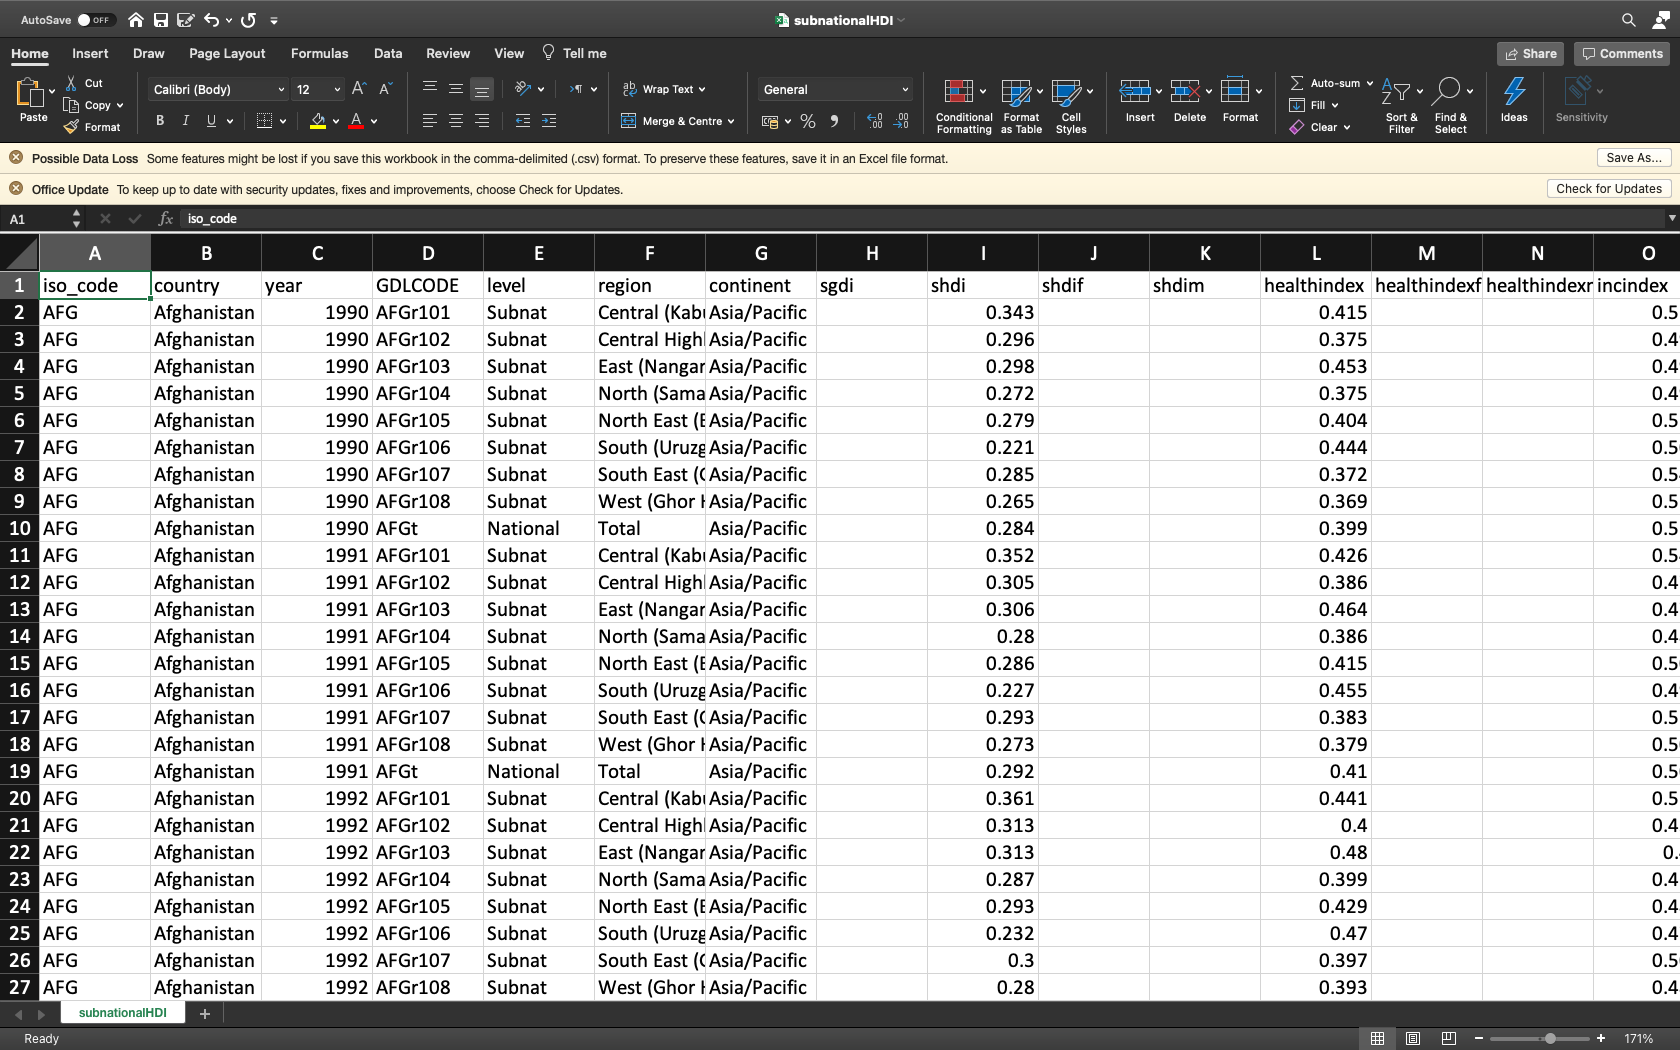
\includegraphics[width=12cm]{ss1.1.png}
\caption{Full dataset containing unnecessary data}
\end{figure}

Therefore, I must write an algorithm to generate a suitable \pil{.csv} file, containing only useful information.

\begin{listing}[H]
\pil{data_processing / process_hdi.py}
\begin{minted}[linenos,breaklines,frame=single,firstnumber=1]{python}
import csv

#retrieve data
with open('data/subnationalHDI.csv', 'r') as file:
    reader = csv.DictReader(file)
\end{minted}
\caption{Initialising \pil{csv} reader}\label{cs:csvReader}
\end{listing}
The \pil{csv} module contains many useful methods for handling \pil{csv} files. I am opening \pil{'data/subnationalHDI.csv'} in read mode, and saving it to the variable \pil{file}. The \pil{with} statement automatically closes the file once I am done with it. The \pil{csv.DictReader} is a class that can read the csv file, and convert each record into a pyton \pil{dict}.

\begin{listing}[H]
\pil{data_processing / process_hdi.py}
\begin{minted}[linenos,breaklines,frame=single,firstnumber=6]{python}
    newcsv = []
    for record in reader:
        if record['year'] == '2022': # the most recent year
            newRecord = {
                "country": record["country"],
                "region": record["region"],
                "code": record["GDLCODE"],
                "hdi": record["shdi"]
            } # only the most useful information
            newcsv.append(newRecord)
            print(newRecord)
\end{minted}
\caption{Refining the HDI Data}\label{cs:refineHDI}
\end{listing}
Here, I define a \pil{list}, \pil{newcsv} to hold all the new (nescessary) records. For each of the records in the full dataset, we must determine if it is from the most recent year (2022). If it is, we make a new record of only the most important information (the region's name, its code (which will be used to uniquely identify it), and its HDI), and append this to \pil{newcsv}.

\begin{figure}[H]
\centering
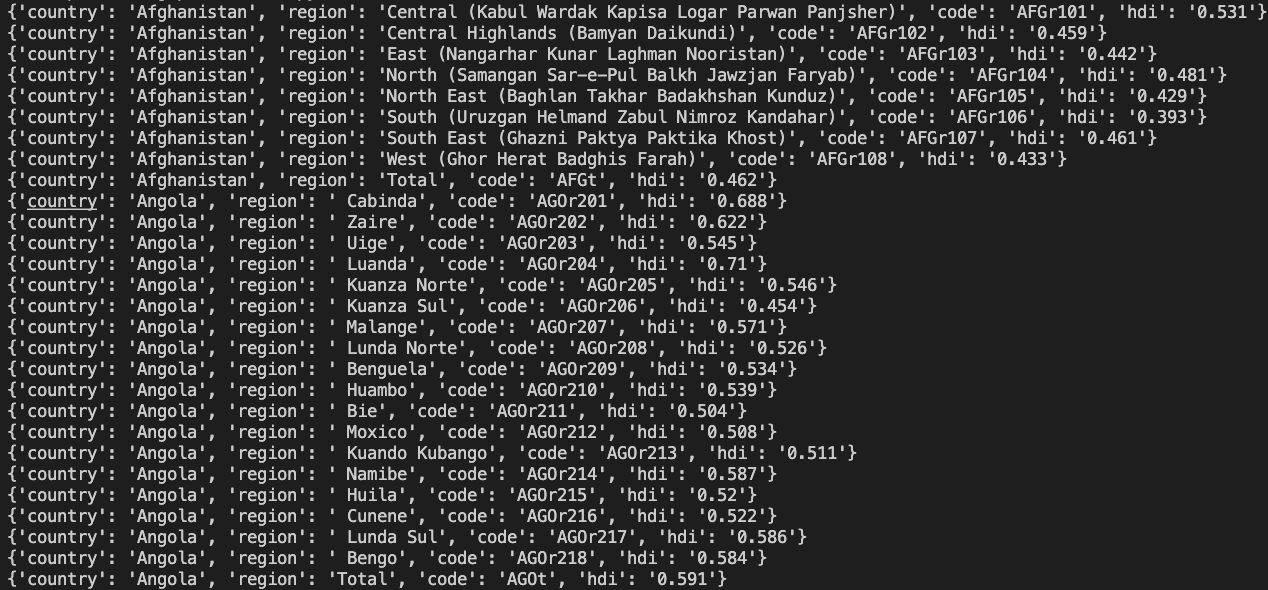
\includegraphics[width=12cm]{ss1.2.png}
\caption{The new records}\label{fig:ss1.2}
\end{figure}
Figure \ref{fig:ss1.2} shows each \pil{newRecord}, which are correct. Therefore, I can now add these to a new \pil{csv} file.

\begin{center}
\csvloop{
    file=data/minitests.csv,
    no head,
    column count=6,
    column names={1=\mtestID, 2=\mtestName, 3=\mtestInputs, 4=\mtestType, 5=\mtestExpectedOutputs, 6=\mtestRealOutputs},
    filter ifthen={\equal{\mtestID}{$t_{1}$}\OR\equal{\mtestID}{\textbf{No.}}},
    before reading={
        \begin{longtable}{|m{1cm}|m{3cm}|m{3cm}|m{2cm}|m{3cm}|m{3cm}|}
        \hline
    },
    command=\csvlinetotablerow,
    late after line=\\\hline,
    after reading={
        \caption{Testing Table for Code Snippets \ref{cs:csvReader} \& \ref{cs:refineHDI}}
        \end{longtable}
    }
}
\end{center}

\begin{listing}[H]
\pil{data_processing / process_hdi.py}
\begin{minted}[linenos,breaklines,frame=single,firstnumber=16]{python}
#write to new csv
with open('data/hdi.csv', 'w') as file:
    field_names = ['country', 'region', 'code', 'hdi']
    writer = csv.DictWriter(file, fieldnames=field_names)
    writer.writeheader()
    for record in newcsv:
        writer.writerow(record)
\end{minted}
\caption{Writing back to \pil{csv}}\label{cs:writingCSV}
\end{listing}
Here, I must open \pil{'data/hdi.csv'} in write mode, to ensure I can make changes to the empty file. The \pil{csv.DictWriter} does the same thing as the \pil{csv.DictReader} but in reverse, so we must specify the field names. After this, we iterate over the \pil{newcsv} \pil{list} and write all of the new records.

\begin{figure}[H]
\centering
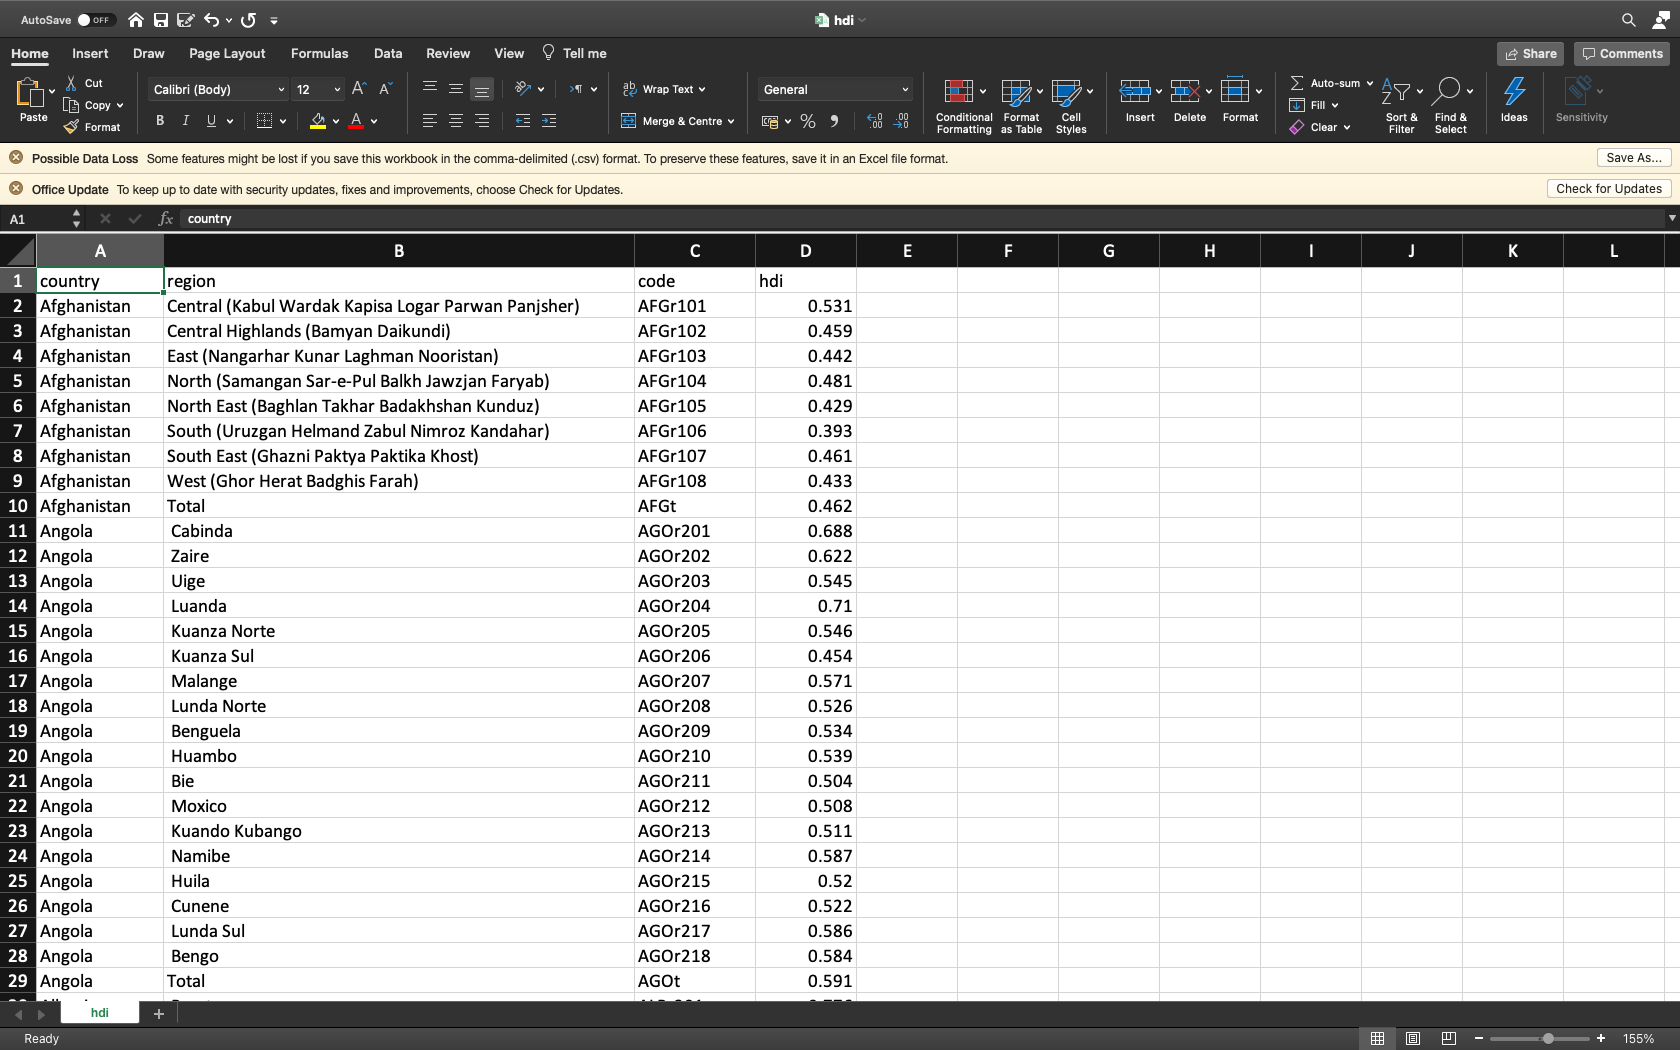
\includegraphics[width=12cm]{ss1.3.png}
\caption{Dataset of only useful HDI information}\label{fig:ss1.3}
\end{figure}
Figure \ref{fig:ss1.3} shows the \pil{csv} file with only the useful information required. Therefore, I can now delete the original \pil{subnatonalHDI.csv} file, as I won't be needing it anymore.

\begin{center}
\csvloop{
    file=data/minitests.csv,
    no head,
    column count=6,
    column names={1=\mtestID, 2=\mtestName, 3=\mtestInputs, 4=\mtestType, 5=\mtestExpectedOutputs, 6=\mtestRealOutputs},
    filter ifthen={\equal{\mtestID}{$t_{2}$}\OR\equal{\mtestID}{\textbf{No.}}},
    before reading={
        \begin{longtable}{|m{1cm}|m{3cm}|m{3cm}|m{2cm}|m{3cm}|m{3cm}|}
        \hline
    },
    command=\csvlinetotablerow,
    late after line=\\\hline,
    after reading={
        \caption{Testing Table for Code Snippet \ref{cs:writingCSV}}
        \end{longtable}
    }
}
\end{center}

\stepcounter{parts}
\subsection{Part \theparts{} -- Collecting OSM Data for a Given Region}\label{sec:get_osm_data}
Next, I need to be able to retrieve the locations of all the objects from OpenStreetMaps, using Overpass Turbo.

\begin{listing}[H]
\pil{data_processing / get_osm_data.py}
\begin{minted}[linenos,breaklines,frame=single,firstnumber=1]{python}
import requests

# makes a request to overpass turbo to get osm data
def get_osm_data(object_type, bounding_coords):
    overpass_url = 'http://overpass-api.de/api/interpreter'
    overpass_query = [
        '(overpass turbo query)'
    ] # placeholder query
    overpass_query = '\n'.join(overpass_query) # concatenates list items into a multi-line string

    response = requests.get(overpass_url, params={'data': overpass_query})
    print(response) # log message, shows the HTTP response code
    data = response.json()
\end{minted}
\caption{Overpass Turbo \pil{GET} Request}\label{cs:overpassRequest}
\end{listing}
Here, I have written a function, \pil{def get_osm_data}, which takes in 2 parameters (the type of object we are looking for, and the region we are looking in). We then must make a query to Overpass Turbo, which often comes in multiple lines. Therefore, I have decided to store each line of the query as a \pil{str}, in a \pil{list}, \pil{overpass_query}, and the join the list with newline characters (\mintinline{python}|'\n'|).

We then make a \pil{GET} request to the URL of Overpass Turbo, passing in the query to ensure we get the correct data. This can be easily done with the \pil{requests} module's \pil{get} function. Once we get a response (hopefully a \pil{200: OK} response, as otherwise something is wrong at Overpass Turbo), we must get the data from it, which will be in a \pil{json} format.

\begin{listing}[H]
\pil{data_processing / get_osm_data.py / def get_osm_data}
\begin{minted}[linenos,breaklines,frame=single,firstnumber=6]{python}
    key_type = ('building' if object_type == 'house' else 'natural' if object_type == 'tree' else 'gambling' if object_type == 'slot_machines' else 'amenity') # get the right key type
    region_poly = ' '.join([' '.join([str(latlong) for latlong in coord]) for coord in bounding_coords]) # converts list of tuples to correct format for overpass turbo
    overpass_query = [
        '[out:json];',
        '(',
        f'   nwr["{key_type}"="{object_type}"](poly:"{region_poly}");',
        ');',
        'out center;'
    ]
\end{minted}
\caption{Overpass Turbo Query}\label{cs:overpassQuery}
\end{listing}

OSM can store data in 3 distinct ways: nodes, ways and relations. A node is a single coordinate, a way is a collection of nodes (which, for example, might represent the outline of a building) and a relation is a collection of nodes, ways or other relations.

The first line of the query \pil{'[out:json];'} specifies that I want the output to be in a \pil{json} format. Using the \pil{'nwr'} command specifies that I want all \textbf{n}odes, \textbf{w}ays and \textbf{r}elations, as what we are looking for could be represented as any of them.

We then must specify that we want only the ways, nodes, and relations of a particular type. Each node/way/relation on OSM has a series of keys, each of which has a value (for example, \pil{"amenity"="restaurant"} would specify that a particular node represents the amenity of a restaurant). The majority of the objects I am looking for are amenities, with a few exceptions. Therefore, I must first determine the correct key before defining the query (as shown on line 6).

We then also need to specify which region we want the ways, nodes and relations to come from. I didn't know how to do this, so I carried out some research on the Overpass Turbo documentation, and found that you can specify a polygon by separating each coordinate with a space (\pil{"La1 Lo1 La2 Lo2 ..."}). This is a different format to how it is passed into the \pil{def get_osm_data} function, so I must first join each of the coordinate pairs with spaces, (\pil{[' '.join(str(latlong) for latlong in coord)]}), and then join each of those with spaces, again before the query is defined (as shown on line 7).

Finally, including \pil{'out center;'} specifies that for each of the ways and relations, their centers should be outputted, instead of their bounding coordinates.

\begin{figure}[H]
\centering
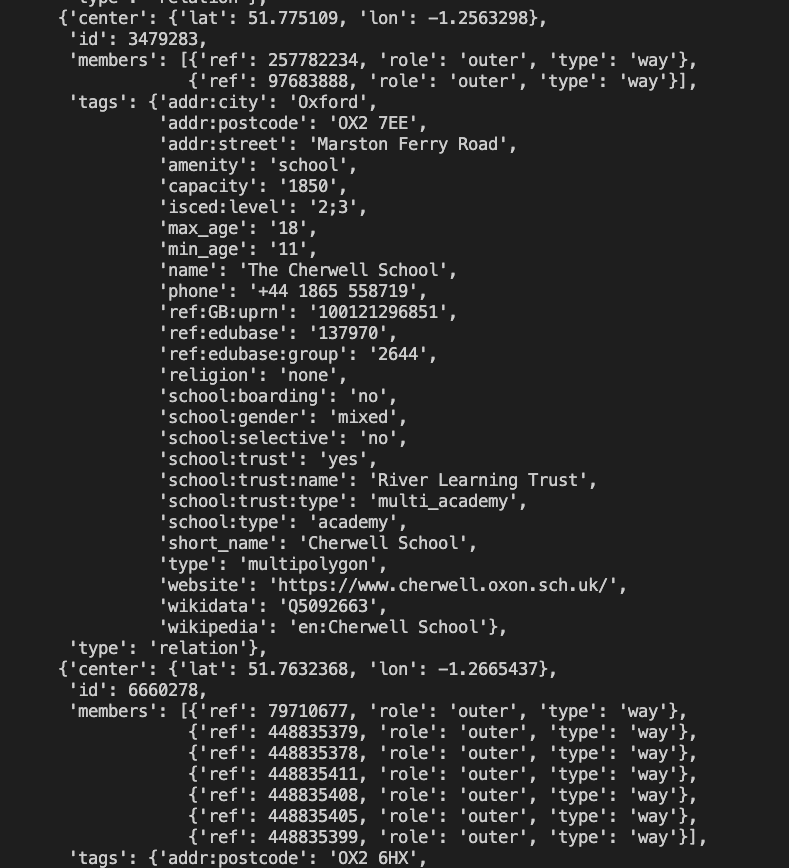
\includegraphics[width=10cm]{ss2.1.png}
\caption{Output of Example Overpass Turbo Query}\label{fig:ss2.1}
\end{figure}
Executing this function, passing in \pil{'school'} for \pil{object_type} and a list of coordinates (in the \pil{list[tuple[float]]} form) of a ring around my local area for \pil{bounding_coords} and printing the what is stored in the variable \pil{data} gives a list of schools in my local area (one of which I go to (and a bit of the next one) is shown in Figure \ref{fig:ss2.1}).

\begin{center}
\csvloop{
    file=data/minitests.csv,
    no head,
    column count=6,
    column names={1=\mtestID, 2=\mtestName, 3=\mtestInputs, 4=\mtestType, 5=\mtestExpectedOutputs, 6=\mtestRealOutputs},
    filter ifthen={\equal{\mtestID}{$T_{1.1}$}\OR\equal{\mtestID}{$T_{1.2}$}\OR\equal{\mtestID}{$T_{1.3}$}\OR\equal{\mtestID}{\textbf{No.}}},
    before reading={
        \begin{longtable}{|m{1cm}|m{3cm}|m{3cm}|m{2cm}|m{3cm}|m{3cm}|}
        \hline
    },
    command=\csvlinetotablerow,
    late after line=\\\hline,
    after reading={
        \caption{$T_{1}$ Testing Table (for Code Snippets \ref{cs:overpassRequest} \& \ref{cs:overpassQuery})}\label{table:t1testing}
        \end{longtable}
    }
}
\end{center}

However, again, there is lots of unnecessary data here (for example names, phone numbers etc.) so we must refine it.

\begin{listing}[H]
\pil{data_processing / get_osm_data.py / def get_osm_data}
\begin{minted}[linenos,breaklines,frame=single,firstnumber=21]{python}
    coords = []
    for nwr in data['elements']:
        if nwr['type'] == 'node':
            coords.append((nwr['lat'], nwr['lon']))
        else: # it is a way or relation
            coords.append((nwr['center']['lat'], nwr['center']['lon']))
    
    return coords
\end{minted}
\caption{Getting a List of Latitude/Longitude Pairs}\label{cs:latlongPairs}
\end{listing}
The objects we are recieving come in a list, which has the key \pil{'elements'}, so I am iterating over \pil{data['elements']}. For each one, we must append only the latitude longitude coordinates (in a \pil{tuple}) to a \pil{list}. If a particular one is stored as a node, then the latitude and longitude coordinates are stored directly, but if it is a way or relation, then they are stored in an additional \pil{dict} with the key \pil{'center'}.

Once we have iterated over each node/way/relation, we can return the \pil{list} of coordinates.

\begin{figure}[H]
\centering
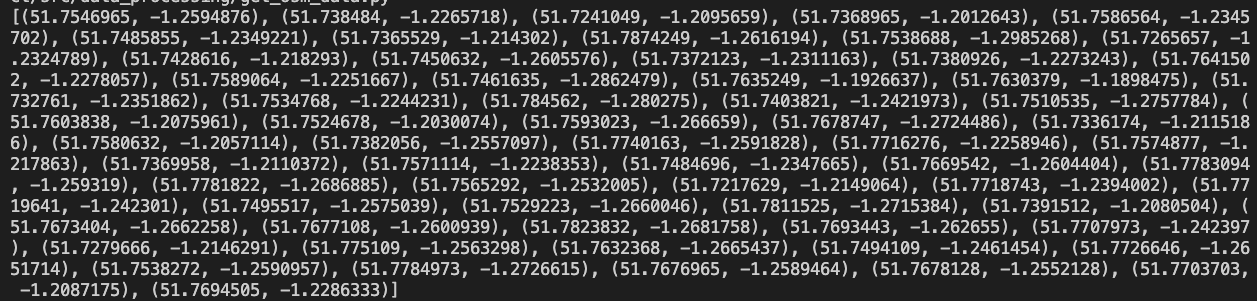
\includegraphics[width=14cm]{ss2.2.png}
\caption{Output of a \pil{list} of Latitude/Longitude pairs}\label{fig:ss2.2}
\end{figure}
Figure \ref{fig:ss2.2} shows the new output of the \pil{def get_osm_data} function with the same input data from Figure \ref{fig:ss2.1}, which is correct.

\begin{center}
\csvloop{
    file=data/minitests.csv,
    no head,
    column count=6,
    column names={1=\mtestID, 2=\mtestName, 3=\mtestInputs, 4=\mtestType, 5=\mtestExpectedOutputs, 6=\mtestRealOutputs},
    filter ifthen={\equal{\mtestID}{$t_{3}$}\OR\equal{\mtestID}{\textbf{No.}}},
    before reading={
        \begin{longtable}{|m{1cm}|m{3cm}|m{3cm}|m{2cm}|m{3cm}|m{3cm}|}
        \hline
    },
    command=\csvlinetotablerow,
    late after line=\\\hline,
    after reading={
        \caption{Testing Table for Code Snippet \ref{cs:latlongPairs}}
        \end{longtable}
    }
}
\end{center}

\stepcounter{parts}
\subsection{Part \theparts{} -- Implementing $A\left(x,y\right)$}\label{sec:aofxyImplementation}
Now, it's time to start calculating the factors from this data. Firstly, the average distance factors.

\begin{listing}[H]
\pil{data_processing / calc_factors.py}
\begin{minted}[linenos,breaklines,frame=single,firstnumber=1]{python}
import numpy as np

EARTH_RADIUS = 6371 # (in km)

# converts angle in degrees to angle in radians
def deg2rad(angle):
    return (np.pi/180)*angle

# finds the distance (in km) along the surface of the earth, between 2 coordinates
def distBetween2Points(p1, p2):
    La1 = deg2rad(p1[0])
    Lo1 = deg2rad(p1[1])
    La2 = deg2rad(p2[0])
    Lo2 = deg2rad(p2[1])
    return EARTH_RADIUS * np.arccos(np.sin(La1)*np.sin(La2) + np.cos(La1)*np.cos(La2)*np.cos(Lo1-Lo2))
\end{minted}
\caption{Finding the Distance between any 2 points}\label{cs:dist2points}
\end{listing}

This code snippet implements equation \ref{eq:dist2points}, which finds the distance along the surface of the Earth, between 2 points (\pil{p1} and \pil{p2}), whose coordinares are given in degrees.

The first thing we need to do, is convert each of these angles into radians, by using the conversion factor $\left(\text{angle in radians}\right)=\frac{\pi}{180}\times\left(\text{angle in degrees}\right)$, and implemented with the function \pil{def deg2rad}.

\begin{center}
\csvloop{
    file=data/minitests.csv,
    no head,
    column count=6,
    column names={1=\mtestID, 2=\mtestName, 3=\mtestInputs, 4=\mtestType, 5=\mtestExpectedOutputs, 6=\mtestRealOutputs},
    filter ifthen={\equal{\mtestID}{$t_{4}$}\OR\equal{\mtestID}{\textbf{No.}}},
    before reading={
        \begin{longtable}{|m{1cm}|m{3cm}|m{3cm}|m{2cm}|m{3cm}|m{3cm}|}
        \hline
    },
    command=\csvlinetotablerow,
    late after line=\\\hline,
    after reading={
        \caption{Testing Table for Code Snippet \ref{cs:dist2points}}
        \end{longtable}
    }
}
\end{center}

We then must calculate the distance with equation \ref{eq:dist2points}, and return it. I am using the module \pil{numpy} for the $\sin$, $\cos$ and $\arccos$ functions, as well as a precise value for $\pi$.

For each of the following tests in $T_{2}$, the 2 points I selected to test were $30^{\circ}$ away from each other, along a great circle. Therefore, the output for all of them should be $\frac{1}{12}\times 2\pi r$, which $\approx 3335.8$ \unit{km}.

\begin{center}
\csvloop{
    file=data/minitests.csv,
    no head,
    column count=6,
    column names={1=\mtestID, 2=\mtestName, 3=\mtestInputs, 4=\mtestType, 5=\mtestExpectedOutputs, 6=\mtestRealOutputs},
    filter ifthen={\equal{\mtestID}{$T_{2.1}$}\OR\equal{\mtestID}{$T_{2.2}$}\OR\equal{\mtestID}{$T_{2.3}$}\OR\equal{\mtestID}{$T_{2.4}$}\OR\equal{\mtestID}{\textbf{No.}}},
    before reading={
        \begin{longtable}{|m{1cm}|m{3cm}|m{3cm}|m{2cm}|m{3cm}|m{3cm}|}
        \hline
    },
    command=\csvlinetotablerow,
    late after line=\\\hline,
    after reading={
        \caption{$T_{2}$ Testing Table (for Code Snippet \ref{cs:dist2points})}\label{table:t2testing}
        \end{longtable}
    }
}
\end{center}

\begin{listing}[H]
\pil{data_processing / calc_factors.py}
\begin{minted}[linenos,breaklines,frame=single,firstnumber=2]{python}
import random
\end{minted}
\pil{data_processing / calc_factors.py}
\begin{minted}[linenos,breaklines,frame=single,firstnumber=18]{python}
# finds the average distance between 2 types of objects, A(x,y)
def averageDistance(x_objects, y_objects, max_x_objects=500):
    if len(x_objects) == 0 or len(y_objects) == 0: # the average distance is undefined
        return None
    if len(x_objects) > max_x_objects: # random sample
        x_objects = random.sample(x_objects, max_x_objects)
\end{minted}
\caption{$A\left(x,y\right)$ Validation}\label{cs:aofxyValidation}
\end{listing}

Here, I am defining the \pil{def averageDistance} function, to calculate $A\left(x,y\right)$. It takes in \pil{x_objects} ($x$), \pil{y_objects} ($y$) and \pil{max_x_objects} as parameters. By default (if nothing is passed in for \pil{max_x_objects}), \pil{max_x_objects} is set to 500, as it was in the flowchart in Figure \ref{fig:aofxy}.

If there are either no $x$-objects, or no $y$-objects, then the average distance between them is undefined, so we must return \pil{None}. When this gets fed into the neural network, it will be replaced by an arbitrarily large number, as (in theory) larger values of $A\left(x,y\right)$ for any $x$, $y$ are ``bad'', and should be decreased.

If there are instead more than (\pil{max_x_objects}) $x$-objects, then we must take a random sample of (\pil{max_x_objects}), as otherwise the function will take too long to execute. To do this, we must first \pil{import random}, and then use its \pil{random.sample()} method.

\begin{center}
\csvloop{
    file=data/minitests.csv,
    no head,
    column count=6,
    column names={1=\mtestID, 2=\mtestName, 3=\mtestInputs, 4=\mtestType, 5=\mtestExpectedOutputs, 6=\mtestRealOutputs},
    filter ifthen={\equal{\mtestID}{$T_{3.1}$}\OR\equal{\mtestID}{$T_{3.2}$}\OR\equal{\mtestID}{$T_{3.3}$}\OR\equal{\mtestID}{$T_{3.4}$}\OR\equal{\mtestID}{\textbf{No.}}},
    before reading={
        \begin{longtable}{|m{1cm}|m{3cm}|m{3cm}|m{2cm}|m{3cm}|m{3cm}|}
        \hline
    },
    command=\csvlinetotablerow,
    late after line=\\\hline,
    after reading={
        \caption{$T_{3}$ Testing Table (for Code Snippet \ref{cs:aofxyValidation})}\label{table:t3testing}
        \end{longtable}
    }
}
\end{center}

\begin{listing}[H]
\pil{data_processing / calc_factors.py / def averageDistance}
\begin{minted}[linenos,breaklines,frame=single,firstnumber=24]{python}
    # iterate over each x_object, and find the closest y_object
    min_dists = []
    for x_object in x_objects:
        dist_to_ys = []
        for y_object in y_objects:
            dist_to_ys.append(distBetween2Points(x_object, y_object))
        min_dists.append(min(dist_to_ys)) # the closest y_object
    return np.mean(min_dists)
\end{minted}
\caption{Calculating $A\left(x,y\right)$}\label{cs:aofxyCalc}
\end{listing}

This code snippet implements the rest of the algorithm to find $A\left(x,y\right)$, as shown in Figure \ref{fig:aofxy}. (We must iterate over each $x$-object, find the closest $y$-object, and return the mean of those distances).

Running this function, passing in the list of schools shown in Figure \ref{fig:ss2.2}, and a list of houses in the same area, returns 0.37311016450362056 \unit{km}, which sounds about right. Running the function again, with the same inputs, but with no random sampling however returns 0.3586665816532994 \unit{km}, which is the true value, but takes longer to calculate. Therefore, in the first run, the random sampling must have (randomly) selected particular houses that happened to be slightly further away from schools than usual (approximately 15 more metres).

\begin{center}
\csvloop{
    file=data/minitests.csv,
    no head,
    column count=6,
    column names={1=\mtestID, 2=\mtestName, 3=\mtestInputs, 4=\mtestType, 5=\mtestExpectedOutputs, 6=\mtestRealOutputs},
    filter ifthen={\equal{\mtestID}{$t_{5}$}\OR\equal{\mtestID}{\textbf{No.}}},
    before reading={
        \begin{longtable}{|m{1cm}|m{3cm}|m{3cm}|m{2cm}|m{3cm}|m{3cm}|}
        \hline
    },
    command=\csvlinetotablerow,
    late after line=\\\hline,
    after reading={
        \caption{Testing Table for Code Snippet \ref{cs:aofxyCalc}}
        \end{longtable}
    }
}
\end{center}

To see the full effect of the random sampling, we can run the function on the same data multiple times, to see the range of values it produces:

\begin{figure}[H]
\centering
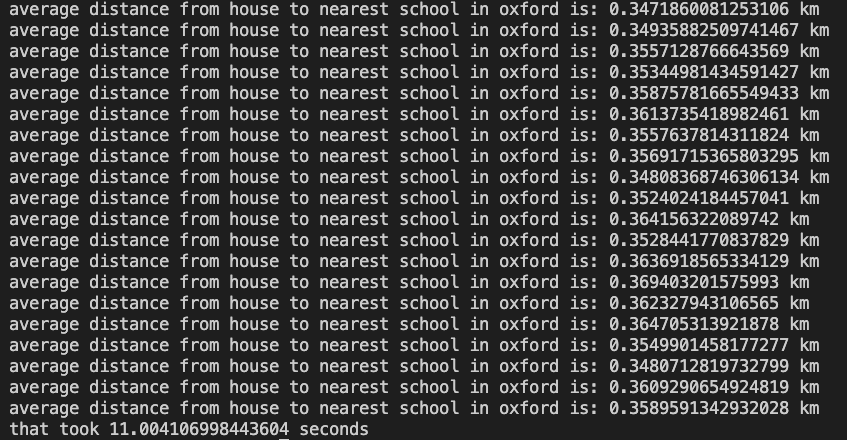
\includegraphics[width=14cm]{ss3.1.png}
\caption{$A\left(x,y\right)$ 20 times, with \pil{max_x_objects} set to 500}\label{fig:ss3.1}
\end{figure}

Figure \ref{fig:ss3.1} shows executing $A\left(x,y\right)$ 20 times, with the same input data as before, and \pil{max_x_objects} set to 500. The value it returns is often correct to 1 significant figure (0.4 \unit{km}), and correct to 2 significant figures about half the time (0.36 \unit{km}). In total, the whole thing took around 11 seconds and so each one took approximately 0.55 seconds.

This is not very accurate, and so I believe we should increase the \pil{max_x_objects}. This will also increase the time for which it takes, so we shouldn't increase it by too much.

\begin{figure}[H]
\centering
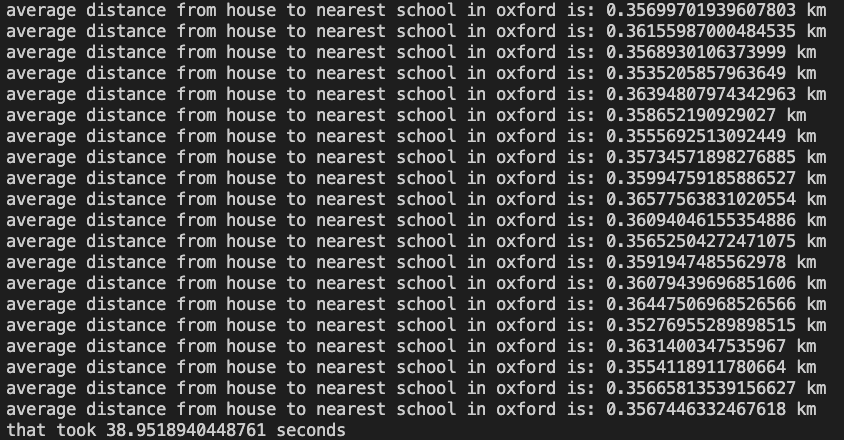
\includegraphics[width=14cm]{ss3.2.png}
\caption{$A\left(x,y\right)$ 20 times, with \pil{max_x_objects} set to 2000}\label{fig:ss3.2}
\end{figure}

Figure \ref{fig:ss3.2} shows executing $A\left(x,y\right)$ 20 times, with the same input data as before, and \pil{max_x_objects} set to 2000. The value it now returns is always correct to 1 significant figure (0.4 \unit{km}), and often correct to 2 significant figures (0.36 \unit{km}). In total, the whole thing took around 39 seconds and so each one took approximately 1.95 seconds. This makes sense, as $A\left(x,y\right)$ should scale linearly with \pil{max_x_objects}, and $0.55\times\frac{2000}{500}\approx 1.95$.

This is a better result, in still a reasonable amount of time, and so I have decided to change the default value for \pil{max_x_value} from \pil{500} to \pil{2000}. The value can of course still be changed at any time, by passing in a different number. When the user comes to predict the HDI of their area in a later prototype, they may be able to change \pil{max_x_objects} with a slider, to make a tradeoff between accuracy and time.

\stepcounter{parts}
\subsection{Part \theparts{} -- Implementing $D\left(x\right)$}\label{sec:dofxImplementation}
Now its time for the harder factors to calculate, the density factors.

First, I decided to make the part of $D\left(x\right)$ that calculates the area of the region a seperate function, as the area will be the same for all density factors of a given area, and so it would be more efficient to calculate it once, beforehand.

\begin{listing}[H]
\pil{data_processing / calc_factors.py}
\begin{minted}[linenos,breaklines,frame=single,firstnumber=33]{python}
# calculates the area (in km^2) of a given region bound by a set of latitude/longitude coordinates
def calcArea(bounding_coords):
    if bounding_coords[0] == bounding_coords[-1]: # if the first and last coordinates are the same, then delete the last one
        bounding_coords.pop(-1)
    # convert lat/lon pairs to 3d position vectors
    bounding_vectors = []
    for coord in bounding_coords:
        La = coord[0]
        Lo = coord[1]
        bounding_vectors.append(np.matrix([
            [np.cos(La)*np.cos(Lo)],
            [np.cos(La)*np.sin(Lo)],
            [np.sin(La)]
        ]))
\end{minted}
\caption{Converting list of bounding coordinates into Column Vectors}\label{cs:dofxVectors}
\end{listing}

Here, I am defining the \pil{def calcArea} function, it takes in the \pil{bounding_coords} as a parameter. The first thing we need to check is if the first and last elements of that list are the same. If they are, then remove the last one, as we don't want to be double-counting a particular vertex.

Next, we must find the absolute position of each coordinate in 3D space, by using equation \ref{eq:convert2vectors} (remembering that $r$ can be set to 1, as the radius of the Earth is irrelevant). As stated before, I am using the \pil{np.matrix} data structure to represent column vectors and matrices.

\begin{center}
\csvloop{
    file=data/minitests.csv,
    no head,
    column count=6,
    column names={1=\mtestID, 2=\mtestName, 3=\mtestInputs, 4=\mtestType, 5=\mtestExpectedOutputs, 6=\mtestRealOutputs},
    filter ifthen={{\equal{\mtestID}{$t_{6}$}\AND\equal{\mtestRealOutputs}{In this example\comma{} (0.276\comma{} 0.445\comma{} 0.851)\comma{} to 3 significant figures}}\OR\equal{\mtestID}{\textbf{No.}}},
    before reading={
        \begin{longtable}{|m{1cm}|m{3cm}|m{3cm}|m{2cm}|m{3cm}|m{3cm}|}
        \hline
    },
    command=\csvlinetotablerow,
    late after line=\\\hline,
    after reading={
        \caption{Testing Table for Code Snippet \ref{cs:dofxVectors}}
        \end{longtable}
    }
}
\end{center}

This is clearly the wrong output. I first thought that maybe equation \ref{eq:convert2vectors} was wrong, but then I checked my working and couldn't find any mistakes. I then realised I hadn't converted from degrees to radians before calculating the vectors.

\begin{listing}[H]
\pil{data_processing / calc_factors.py / def calcArea}
\begin{minted}[linenos,breaklines,frame=single,firstnumber=40]{python}
        La = deg2rad(coord[0])
        Lo = deg2rad(coord[1])
\end{minted}
\caption{Coverting from Degrees to Radians}\label{cs:dofxRadians}
\end{listing}

\begin{center}
\csvloop{
    file=data/minitests.csv,
    no head,
    column count=6,
    column names={1=\mtestID, 2=\mtestName, 3=\mtestInputs, 4=\mtestType, 5=\mtestExpectedOutputs, 6=\mtestRealOutputs},
    filter ifthen={{\equal{\mtestID}{$t_{6}$}\AND\equal{\mtestRealOutputs}{In this example\comma{} (0.5\comma{} 0.5\comma{} 0.707)\comma{} to 3 significant figures\comma{} As Expected}}\OR\equal{\mtestID}{\textbf{No.}}},
    before reading={
        \begin{longtable}{|m{1cm}|m{3cm}|m{3cm}|m{2cm}|m{3cm}|m{3cm}|}
        \hline
    },
    command=\csvlinetotablerow,
    late after line=\\\hline,
    after reading={
        \caption{Testing Table for Code Snippet \ref{cs:dofxRadians}}
        \end{longtable}
    }
}
\end{center}

This now produces correct vectors. We now must iterate over each vertex, and find its anticlockwise angle.

\begin{listing}[H]
\pil{data_processing / calc_factors.py / def calcArea}
\begin{minted}[linenos,breaklines,frame=single,firstnumber=47]{python}
    # iterate over each vertex and find its anticlockwise angle
    for vertex_index, vertex in enumerate(bounding_vectors):
        prev_vertex = bounding_vectors[vertex_index-1]
        next_vertex = bounding_vectors[0 if vertex_index == len(bounding_vectors)-1 else vertex_index+1]
        La = deg2rad(bounding_coords[vertex_index][0])
        Lo = deg2rad(bounding_coords[vertex_index][1])
        # define the rotation and translation matrices
        rotation_matrix_z = np.matrix([
            [np.cos(-Lo), -np.sin(-Lo), 0],
            [np.sin(-Lo), np.cos(-Lo), 0],
            [0, 0, 1]
        ])
        rotation_matrix_y = np.matrix([
            [np.cos(La-np.pi/2), 0, np.sin(La-np.pi/2)],
            [0, 1, 0],
            [-np.sin(La-np.pi/2), 0, np.cos(La-np.pi/2)]
        ])
        translation_vector = np.matrix([
            [0],
            [0],
            [-1]
        ])
\end{minted}
\caption{Defining Key Variables in calculating area}\label{cs:dofxDefinitions}
\end{listing}

Firstly, we need to get the positions 2 vertices adjacent to the one we are considering. To get the previous one, we can just subtract 1 from the index of the current one, (as in the case that we are considering the first vertex, the index \pil{-1} refers to the last element in a list, which is the previous one in the shape). To get the next vertex, the index will usually be 1 more than the current index, except for when we are considering the final vertex, as the next one will be the first vertex.

We then must find the latitude and longitude of the current vertex, so that we can rotate the plane tangent to it to be the $xy$-plane. Luckily, \pil{bounding_coords} and \pil{bounding_vectors} have the same indices, so we just need to pass the \pil{bounding_coord} at the index \pil{vertex_index} through the \pil{def deg2rad} function to get what we need.

Finally, we must define the 3 matries used to transform the plane into the $xy$-plane, as shown in equations \ref{eq:transformCoordsStart} to \ref{eq:transformCoordsEnd}.

\begin{listing}[H]
\pil{data_processing / calc_factors.py / def calcArea}
\begin{minted}[linenos,breaklines,frame=single,firstnumber=69]{python}
        # rotate and translate the plane tangent to the vertex such that it is the xy-plane
        prev_vertex = np.matmul(rotation_matrix_y, np.matmul(rotation_matrix_z, prev_vertex)) + translation_vector
        vertex = np.matmul(rotation_matrix_y, np.matmul(rotation_matrix_z, vertex)) + translation_vector
        next_vertex = np.matmul(rotation_matrix_y, np.matmul(rotation_matrix_z, next_vertex)) + translation_vector
        # project onto the xy-plane
        prev_vertex[2][0] = 0
        next_vertex[2][0] = 0
\end{minted}
\caption{Rotating the plane tangent to each vertex}\label{cs:dofxRotations}
\end{listing}

Now we must transform each of these vertices, using the matrices we just defined. As stated before, the first is to perform a rotation about the $z$-axis, such that it is parrallel to the $y$-axis, the second is to perform a rotation about the $y$-axis such that it is parrallel to the $x$-axis (and hence a translation of the $xy$-plane), and the third is to translate it onto the $xy$-plane.

Then, to project the previous and next vertices onto the $xy$-plane, we can just set their $z$-coordinates to 0. This is at index \pil{[2][0]}, as $z$ is the third axis (second with 0-indexing) and the column vectors are stored as a matrix, so each item in the column vector is actually an array (hence the \pil{[0]} index).

\begin{center}
\csvloop{
    file=data/minitests.csv,
    no head,
    column count=6,
    column names={1=\mtestID, 2=\mtestName, 3=\mtestInputs, 4=\mtestType, 5=\mtestExpectedOutputs, 6=\mtestRealOutputs},
    filter ifthen={\equal{\mtestID}{$t_{7}$}\OR\equal{\mtestID}{$t_{8}$}\OR\equal{\mtestID}{$t_{9}$}\OR\equal{\mtestID}{\textbf{No.}}},
    before reading={
        \begin{longtable}{|m{1cm}|m{3cm}|m{3cm}|m{2cm}|m{3cm}|m{3cm}|}
        \hline
    },
    command=\csvlinetotablerow,
    late after line=\\\hline,
    after reading={
        \caption{Testing Table for Code Snippets \ref{cs:dofxDefinitions} \& \ref{cs:dofxRotations}}
        \end{longtable}
    }
}
\end{center}

\begin{listing}[H]
\pil{data_processing / calc_factors.py / def calcArea}
\begin{minted}[linenos,breaklines,frame=single,firstnumber=48]{python}
    anticlockwise_angles = []
\end{minted}
\pil{data_processing / calc_factors.py / def calcArea}
\begin{minted}[linenos,breaklines,frame=single,firstnumber=77]{python}
        # calculate anticlockwise angle between the vectors
        prev_to_current = vertex - prev_vertex
        current_to_next = next_vertex - vertex
        anticlockwise_angle = np.arctan2((prev_to_current.item(1,0)*current_to_next.item(2,0) - prev_to_current.item(2,0)*current_to_next.item(1,0)) - (prev_to_current.item(2,0)*current_to_next.item(0,0) - prev_to_current.item(0,0)*current_to_next.item(2,0)) + (prev_to_current.item(0,0)*current_to_next.item(1,0) - prev_to_current.item(1,0)*current_to_next.item(0,0)), prev_to_current.item(0,0)*current_to_next.item(0,0) + prev_to_current.item(1,0)*current_to_next.item(1,0) + prev_to_current.item(2,0)*current_to_next.item(2,0))
        anticlockwise_angles.append(anticlockwise_angle)
\end{minted}
\caption{Finding the anticlockwise angles}\label{cs:dofxAnticlockwiseAngles}
\end{listing}

Now we must find the anticlockwise angle between the vertices. First, we find the vector to get from the previous vertex to the current vertex, and the vector to get from the current vertex to the next vertex, and then use equation \ref{eq:calcClockwiseAngle} to find the anticlockwise angle.

\pil{np.arctan2} is the 2-argument form of the arctan function, giving a range of $-\pi$ to $\pi$, instead of the regular $-\frac{\pi}{2}$ to $\frac{\pi}{2}$.

As we will want to find the sum of these anticlockwise angles, we must first declare a \pil{list} before the \pil{for} loop (started in Code Snippet \ref{cs:dofxDefinitions}), and then append each anticlockwise angle to it.

\begin{center}
\csvloop{
    file=data/minitests.csv,
    no head,
    column count=6,
    column names={1=\mtestID, 2=\mtestName, 3=\mtestInputs, 4=\mtestType, 5=\mtestExpectedOutputs, 6=\mtestRealOutputs},
    filter ifthen={\equal{\mtestID}{$t_{10}$}\OR\equal{\mtestID}{\textbf{No.}}},
    before reading={
        \begin{longtable}{|m{1cm}|m{3cm}|m{3cm}|m{2cm}|m{3cm}|m{3cm}|}
        \hline
    },
    command=\csvlinetotablerow,
    late after line=\\\hline,
    after reading={
        \caption{Testing Table for Code Snippet \ref{cs:dofxAnticlockwiseAngles}}
        \end{longtable}
    }
}
\end{center}

\begin{listing}[H]
\pil{data_processing / calc_factors.py / def calcArea}
\begin{minted}[linenos,breaklines,frame=single,firstnumber=82]{python}
    # find the interior angles from the anticlockwise angles
    sum_anticlockwise_angles = sum(anticlockwise_angles)
    if sum_anticlockwise_angles == 0:
        return None
    if sum_anticlockwise_angles < 0:
        anticlockwise_angles = [-1*angle for angle in anticlockwise_angles]
    interior_angles = [np.pi-angle for angle in anticlockwise_angles]
    # return the area
    num_edges = len(bounding_coords)
    return (EARTH_RADIUS ** 2) * (sum(interior_angles) - np.pi*(num_edges-2))
\end{minted}
\caption{Calculating the Area}\label{cs:dofxArea}
\end{listing}

This code snippet implements the bottom half of the flowchart for $D\left(x\right)$, in Figure \ref{fig:dofx}. We find the sum of the anticlockwise angles, if it is 0, then the shape must be invalid and so we \pil{return None}.

If the sum is negative, then the shape must have been drawn the wrong way around, and so we must multiply each of the anticlockwise angles by $-1$, before continuing, which can be done with a list comprehension.

Then, to calculate the interior angles, we subtract each angle from $\pi$, again using a list comprehension. Finally, to calculate the area of the region we use equation \ref{eq:areaRegion}. To find the number of edges of the shape, we just count the number of vertices, as they will always be the same thing.

\begin{center}
\csvloop{
    file=data/minitests.csv,
    no head,
    column count=6,
    column names={1=\mtestID, 2=\mtestName, 3=\mtestInputs, 4=\mtestType, 5=\mtestExpectedOutputs, 6=\mtestRealOutputs},
    filter ifthen={{\equal{\mtestID}{$T_{4.4}$}\AND\equal{\mtestRealOutputs}{Some large area}}\OR\equal{\mtestID}{$T_{4.1}$}\OR\equal{\mtestID}{$T_{4.2}$}\OR\equal{\mtestID}{$T_{4.3}$}\OR\equal{\mtestID}{\textbf{No.}}},
    before reading={
        \begin{longtable}{|m{1cm}|m{3cm}|m{3cm}|m{2cm}|m{3cm}|m{3cm}|}
        \hline
    },
    command=\csvlinetotablerow,
    late after line=\\\hline,
    after reading={
        \caption{$T_{4}$ Testing Table (for Code Snippet \ref{cs:dofxArea})}\label{table:t4testing}
        \end{longtable}
    }
}
\end{center}

For the areas drawn clockwise and anticlockwise, I used the same area that I used to get the data about houses and schools in the $A\left(x,y\right)$ section, which was a polygon around Oxford. The areas they returned were about right, after researching the true area of Oxford. My values turned out greater as I was drawing \textit{around} Oxford. The discrepancy between the clockwise and anticlockwise values is most likely due to floating point arithmetic and calculating things in different orders.

For the area drawn in multiple loops around the Earth, I again used the same area of Oxford, except some of the coordinates had multiples of 360 added to them. Again, the discrepancy between values can be explained by floating point binary.

\begin{figure}[H]
\centering
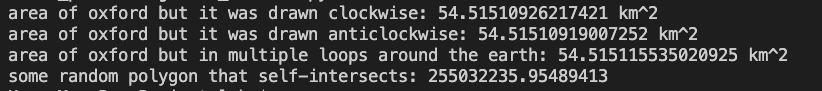
\includegraphics[width=14cm]{ss4.1.png}
\caption{Area of Oxford, with an Invalid Self-Intersection}\label{fig:ss4.1}
\end{figure}

The area that self-intersects must also have not worked as a result of floating point binary. When inspecting the sum of the anticlockwise angles, I found that it was very close to 0, but not quite. Therefore, I must round the sum of the anticlockwise angles before seeing if it is 0.

\begin{listing}[H]
\pil{data_processing / calc_factors.py / def calcArea}
\begin{minted}[linenos,breaklines,frame=single,firstnumber=83]{python}
    sum_anticlockwise_angles = round(sum(anticlockwise_angles), 5)
\end{minted}
\caption{Rounding the sum of anticlockwise angles}\label{cs:dofxRounding}
\end{listing}

5 decimal places should be enough to determine if it is supposed to be 0, while not affecting anything that shouldn't be 0.

\begin{center}
\csvloop{
    file=data/minitests.csv,
    no head,
    column count=6,
    column names={1=\mtestID, 2=\mtestName, 3=\mtestInputs, 4=\mtestType, 5=\mtestExpectedOutputs, 6=\mtestRealOutputs},
    filter ifthen={{\equal{\mtestID}{$T_{4.4}$}\AND\equal{\mtestRealOutputs}{As Expected}}\OR\equal{\mtestID}{\textbf{No.}}},
    before reading={
        \begin{longtable}{|m{1cm}|m{3cm}|m{3cm}|m{2cm}|m{3cm}|m{3cm}|}
        \hline
    },
    command=\csvlinetotablerow,
    late after line=\\\hline,
    after reading={
        \caption{Testing Table for Code Snippet \ref{cs:dofxRounding}}
        \end{longtable}
    }
}
\end{center}

\begin{figure}[H]
\centering
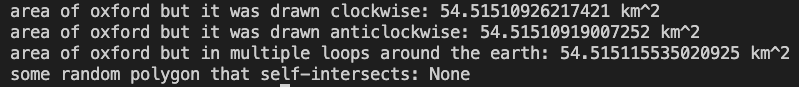
\includegraphics[width=14cm]{ss4.2.png}
\caption{Area of Oxford, with a Valid Self-Intersection}\label{fig:ss4.2}
\end{figure}

Finally, all that is left to do is calculate $D\left(x\right)$.

\begin{listing}[H]
\pil{data_processing / calc_factors.py}
\begin{minted}[linenos,breaklines,frame=single,firstnumber=93]{python}
# finds the density of a type of object, D(x)
def density(x_objects, area):
    return len(x_objects)/area
\end{minted}
\caption{Calculating $D\left(x\right)$}\label{cs:dofx}
\end{listing}

$D\left(x\right)$ is given by the number of $x$-objects per unit area, so we can just find the length of the \pil{x_objects} list and divide by the area to get our answer.

\begin{center}
\csvloop{
    file=data/minitests.csv,
    no head,
    column count=6,
    column names={1=\mtestID, 2=\mtestName, 3=\mtestInputs, 4=\mtestType, 5=\mtestExpectedOutputs, 6=\mtestRealOutputs},
    filter ifthen={\equal{\mtestID}{$t_{11}$}\OR\equal{\mtestID}{\textbf{No.}}},
    before reading={
        \begin{longtable}{|m{1cm}|m{3cm}|m{3cm}|m{2cm}|m{3cm}|m{3cm}|}
        \hline
    },
    command=\csvlinetotablerow,
    late after line=\\\hline,
    after reading={
        \caption{Testing Table for Code Snippet \ref{cs:dofx}}
        \end{longtable}
    }
}
\end{center}

\begin{figure}[H]
\centering

\includegraphics[width=14cm]{ss4.3.png}
\caption{$D\left(\text{School}\right)$ for Oxford}\label{fig:ss4.3}
\end{figure}

\stepcounter{parts}
\subsection{Part \theparts{} -- Iterating over each Subnational Region}\label{sec:iterateRegions}

Now it is time to finally compile all of our training data. We first must be able to find all of the required factors for any given area.

\begin{listing}[H]
\pil{data_processing / calc_factors.py}
\begin{minted}[linenos,breaklines,frame=single,firstnumber=3]{python}
from get_osm_data import get_osm_data
\end{minted}
\pil{data_processing / calc_factors.py}
\begin{minted}[linenos,breaklines,frame=single,firstnumber=98]{python}
# finds all the factors for a given region
def getAllFactors(region):
    # retrieve all relevant osm data
    object_types = ['house', 'school', 'hospital', 'pharmacy', 'restaurant', 'place_of_worship', 'bank', 'slot_machines', 'fast_food', 'toilets', 'police', 'university', 'library', 'post_box', 'vending_machine', 'bench', 'tree']
    all_objects = {}
    for object_type in object_types:
        print(f'getting {object_type} data...') # log message
        all_objects[object_type] = get_osm_data(object_type, region)
\end{minted}
\caption{Retrieving All OSM Data}\label{cs:retrieveAllData}
\end{listing}

To do this, I have defined a function, \pil{def getAllFactors}, which takes in a region (in the \pil{list[tuple[float]]} format), and returns a \pil{dict} of all the factors. We must first retrieve all of the relevant data from OSM (using the \pil{def get_osm_data} function implemented in Section \ref{sec:get_osm_data}).

Here, I define a list of all the object types needed for all of the factors, and an empty dictionary. For each of the object types, a key is created in the dictionary, with the value being the returned \pil{list} of latitude and longitude coordinates

I am also printing a log message, as some of these fetches may take a long time, and so it is useful to keep track of where we are in the process

\begin{center}
\csvloop{
    file=data/minitests.csv,
    no head,
    column count=6,
    column names={1=\mtestID, 2=\mtestName, 3=\mtestInputs, 4=\mtestType, 5=\mtestExpectedOutputs, 6=\mtestRealOutputs},
    filter ifthen={\equal{\mtestID}{$t_{12}$}\OR\equal{\mtestID}{\textbf{No.}}},
    before reading={
        \begin{longtable}{|m{1cm}|m{3cm}|m{3cm}|m{2cm}|m{3cm}|m{3cm}|}
        \hline
    },
    command=\csvlinetotablerow,
    late after line=\\\hline,
    after reading={
        \caption{Testing Table for Code Snippet \ref{cs:retrieveAllData}}
        \end{longtable}
    }
}
\end{center}

\begin{figure}[H]
\centering
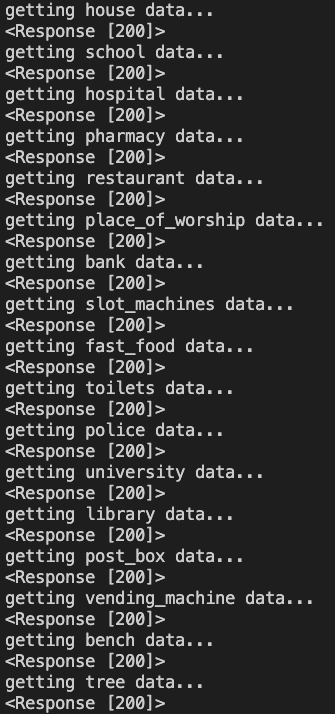
\includegraphics[width=6cm]{ss5.1.png}
\caption{Log messages for Collecting data for all objects}\label{fig:ss5.1}
\end{figure}

Now we must calculate each factor with this information.

\begin{listing}[H]
\pil{data_processing / calc_factors.py / def getAllFactors}
\begin{minted}[linenos,breaklines,frame=single,firstnumber=106]{python}
    # return a dictionary of all the factors
    print('calculating area...') # log message
    area = calcArea(region)
    print('calculating factors...') # log message
    return {
        "A(House School)": averageDistance(all_objects['house'], all_objects['school']),
        "A(House Hospital)": averageDistance(all_objects['house'], all_objects['hospital']),
        "A(House Pharmacy)": averageDistance(all_objects['house'], all_objects['pharmacy']),
        "A(House Restaurant)": averageDistance(all_objects['house'], all_objects['restaurant']),
        "A(School Hospital)": averageDistance(all_objects['school'], all_objects['hospital']),
        "A(Police Hospital)": averageDistance(all_objects['police'], all_objects['hospital']),
        "A(House Place of Worship)": averageDistance(all_objects['house'], all_objects['place_of_worship']),
        "A(Bank Slot Machine)": averageDistance(all_objects['bank'], all_objects['slot_machines']),
        "A(Fast-Food Place Toilet)": averageDistance(all_objects['fast_food'], all_objects['toilets']),
        "A(House Police)": averageDistance(all_objects['house'], all_objects['police']),
        "A(University Library)": averageDistance(all_objects['university'], all_objects['library']),
        "A(House Library)": averageDistance(all_objects['house'], all_objects['library']),
\end{minted}
\caption{Calculating All Average Distance Factors}\label{cs:calcAllAFactors}
\end{listing}

Here, I am returning a \pil{dict} witha key for each factor. For the average distance factors, we can just pass the relevant data into the \pil{def averageDistance} function (implemented in Section \ref{sec:aofxyImplementation}).

The factor names don't have a comma between the 2 parameters of the $A$ function, as that would mess up the \pil{csv} headers.

\begin{listing}[H]
\pil{data_processing / calc_factors.py / def getAllFactors}
\begin{minted}[linenos,breaklines,frame=single,firstnumber=123]{python}
        "D(School)": density(all_objects['school'], area),
        "D(Hospital)": density(all_objects['hospital'], area),
        "D(Pharmacy)": density(all_objects['pharmacy'], area),
        "D(Police)": density(all_objects['police'], area),
        "D(Library)": density(all_objects['library'], area),
        "D(Toilet)": density(all_objects['toilets'], area),
        "D(Restaurant)": density(all_objects['restaurant'], area),
        "D(Place of Worship)": density(all_objects['place_of_worship'], area),
        "D(Post Box)": density(all_objects['post_box'], area),
        "D(Vending Machine)": density(all_objects['vending_machine'], area),
        "D(Bench)": density(all_objects['bench'], area),
        "D(Tree)": density(all_objects['tree'], area),
    }
\end{minted}
\caption{Calculating All Density Factors}\label{cs:calcAllDFactors}
\end{listing}

For the density factors, we can just pass the relevant data into the \pil{def density} function (implemented in Section \ref{sec:dofxImplementation}), along with the area of the region. The area of the region must therefore be calculated before, by using the \pil{def calcArea} function (also implemented in Section \ref{sec:dofxImplementation}).

\begin{center}
\csvloop{
    file=data/minitests.csv,
    no head,
    column count=6,
    column names={1=\mtestID, 2=\mtestName, 3=\mtestInputs, 4=\mtestType, 5=\mtestExpectedOutputs, 6=\mtestRealOutputs},
    filter ifthen={\equal{\mtestID}{$t_{13}$}\OR\equal{\mtestID}{\textbf{No.}}},
    before reading={
        \begin{longtable}{|m{1cm}|m{3cm}|m{3cm}|m{2cm}|m{3cm}|m{3cm}|}
        \hline
    },
    command=\csvlinetotablerow,
    late after line=\\\hline,
    after reading={
        \caption{Testing Table for Code Snippets \ref{cs:calcAllAFactors} \& \ref{cs:calcAllDFactors}}
        \end{longtable}
    }
}
\end{center}

\begin{figure}[H]
\centering
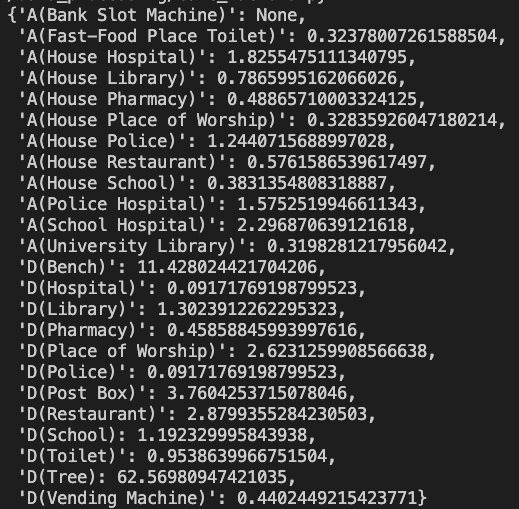
\includegraphics[width=9cm]{ss5.2.png}
\caption{Example all factors \pil{dict} for Oxford}\label{fig:ss5.2}
\end{figure}

Figure \ref{fig:ss5.2} shows the output of the \pil{def getAllFactors} function for the same region I have been testing in previously (a rough ring around Oxford).

I now need a list of all of the subnational regions (that is, a \pil{list} of bounding coordinates for each one). As stated before, I will also download this from the Global Data Lab \cite{regionBorders}.

The full dataset is a shapefile \pil{.shp}, which I didn't know how to read. After researching the problem, I found a StackOverflow solution \cite{stackOverflowConvertShapefile} on how to convert a shapefile into a \pil{.json} file, which I do know how to read.

\begin{listing}[H]
(This code has been adapted from this StackOverflow solution: \cite{stackOverflowConvertShapefile}) \\
\pil{data_processing / process_shapefile.py}
\begin{minted}[linenos,breaklines,frame=single,firstnumber=1]{python}
import shapefile
import json

# read records of shapefile
reader = shapefile.Reader("data/shapefiles/GDL Shapefiles V6.3 large.shp")
fields = reader.fields[1:]
field_names = [field[0] for field in fields]
data = []
for shape_record in reader.shapeRecords():
    print(shape_record.record) # log message
    data.append({
        "type": "Feature",
        "geometry": shape_record.shape.__geo_interface__,
        "properties": dict(zip(field_names, shape_record.record))
    })

# write data to file
print('writing to file...') # log message
with open("data/region_coords.json", "w") as file:
    json.dump(data, file)
print('done!') # log message
\end{minted}
\caption{Processing the Shapefile}\label{cs:processShapefile}
\end{listing}

Code Snippet \ref{cs:processShapefile} shows the code from the StackOverflow solution \cite{stackOverflowConvertShapefile}, with some slight modifications.

First, we must \pil{import shapefile} and \pil{import json}, to be able to handle the 2 different types of files. It then looks like we define a \pil{reader}, similar to what we did with the \pil{.csv} file.

It appears that shapefiles are similarly structured to databases, as we have a set of fields, and records containing values for each field. To turn this into a \pil{.json} file, we can iterate over each record, create a dictionary out of it, and append it to a \pil{list}. Once we have a full list, we can write it to a \pil{.json} file.

\begin{figure}[H]
\centering
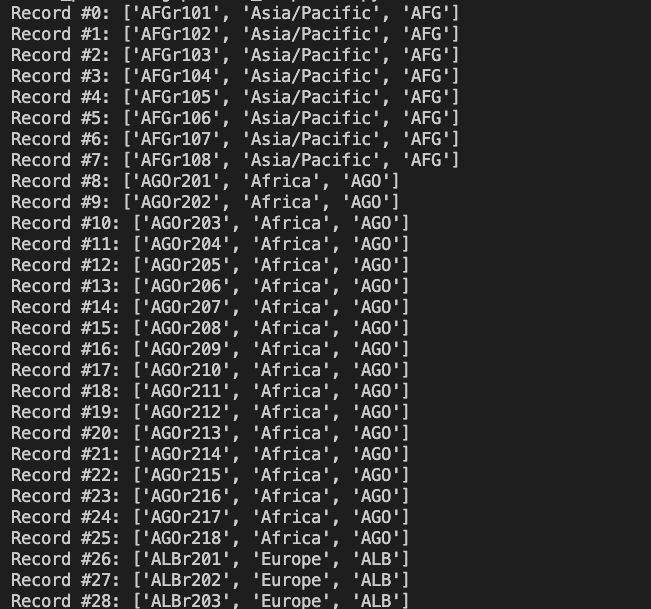
\includegraphics[width=9cm]{ss5.3.png}
\caption{Each record of the shapefile}\label{fig:ss5.3}
\end{figure}

Figure \ref{fig:ss5.3} shows each record being read from the shapefile. The list of coordinates does not appear to be here, so that must be what is stored in the \pil{shape_record.shape.__geo_interface__} attribute.

\begin{center}
\csvloop{
    file=data/minitests.csv,
    no head,
    column count=6,
    column names={1=\mtestID, 2=\mtestName, 3=\mtestInputs, 4=\mtestType, 5=\mtestExpectedOutputs, 6=\mtestRealOutputs},
    filter ifthen={\equal{\mtestID}{$t_{14}$}\OR\equal{\mtestID}{\textbf{No.}}},
    before reading={
        \begin{longtable}{|m{1cm}|m{3cm}|m{3cm}|m{2cm}|m{3cm}|m{3cm}|}
        \hline
    },
    command=\csvlinetotablerow,
    late after line=\\\hline,
    after reading={
        \caption{Testing Table for Code Snippet \ref{cs:processShapefile}}
        \end{longtable}
    }
}
\end{center}

\begin{figure}[H]
\centering
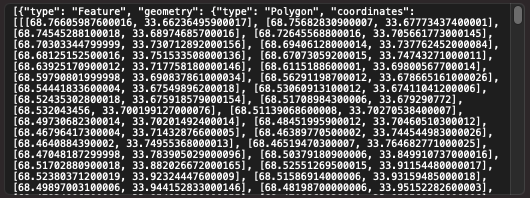
\includegraphics[width=14cm]{ss5.4.png}
\caption{Sample of the resulting \pil{.json} file}\label{fig:ss5.4}
\end{figure}

Now it is time to execute the \pil{def getAllFactors} function on each of these regions, to make our training data.

\begin{listing}[H]
\pil{data_processing / compile_data.py}
\begin{minted}[linenos,breaklines,frame=single,firstnumber=1]{python}
import json
import csv

print('reading files...') # log message
# read json file
with open('data/region_coords.json', 'r') as file:
    regionData = json.load(file)

# read csv file
with open('data/hdi.csv', 'r') as file:
    reader = csv.DictReader(file)
    hdiData = []
    for record in reader:
        hdiData.append(record)
\end{minted}
\caption{Reading the Region \& HDI files}\label{cs:readingRegions}
\end{listing}

Here, I am reading the 2 files I need, to get the region data and the HDI data. We must first \pil{import json} and \pil{import csv}, as those are the 2 types of file we are dealing with. Reading these files is done in the same way as before, by defining a \pil{csv.DictReader} of the file.

\begin{center}
\csvloop{
    file=data/minitests.csv,
    no head,
    column count=6,
    column names={1=\mtestID, 2=\mtestName, 3=\mtestInputs, 4=\mtestType, 5=\mtestExpectedOutputs, 6=\mtestRealOutputs},
    filter ifthen={\equal{\mtestID}{$t_{15}$}\OR\equal{\mtestID}{\textbf{No.}}},
    before reading={
        \begin{longtable}{|m{1cm}|m{3cm}|m{3cm}|m{2cm}|m{3cm}|m{3cm}|}
        \hline
    },
    command=\csvlinetotablerow,
    late after line=\\\hline,
    after reading={
        \caption{Testing Table for Code Snippet \ref{cs:readingRegions}}
        \end{longtable}
    }
}
\end{center}

\begin{listing}[H]
\pil{data_processing / compile_data.py}
\begin{minted}[linenos,breaklines,frame=single,firstnumber=16]{python}
SKIP_THE_FIRST = 0

# iterate over each region
for region_number, region in enumerate(regionData):
    if region_number < SKIP_THE_FIRST:
        continue
    print(f'Processing {region["properties"]["gdlcode"]}...') # log message
\end{minted}
\caption{Iterating over each region}\label{cs:iterateRegions}
\end{listing}

This code will iterate over each \pil{region}, contained within the \pil{region_coords.json} file, by making use of a \pil{for} loop. Carrying this out is likely to take an extremely long time, and so I might want to pause the process, or if it crashes for some reason, I won't want to start from the beginning. Therefore, I have defined a variable, \pil{SKIP_THE_FIRST} $n$, which will tell the program to not calculate the first $n$ regions. We can implement this by using the \pil{enumerate} function, which will allow for us to keep count, and the \pil{continue} key word, which will skip the remaining code of the \pil{for} loop, and continue to the next iteration.

\begin{center}
\csvloop{
    file=data/minitests.csv,
    no head,
    column count=6,
    column names={1=\mtestID, 2=\mtestName, 3=\mtestInputs, 4=\mtestType, 5=\mtestExpectedOutputs, 6=\mtestRealOutputs},
    filter ifthen={\equal{\mtestID}{$t_{16}$}\AND\equal{\mtestExpectedOutputs}{Starts on region $n+1$}\OR\equal{\mtestID}{\textbf{No.}}},
    before reading={
        \begin{longtable}{|m{1cm}|m{3cm}|m{3cm}|m{2cm}|m{3cm}|m{3cm}|}
        \hline
    },
    command=\csvlinetotablerow,
    late after line=\\\hline,
    after reading={
        \caption{Testing Table for Code Snippet \ref{cs:iterateRegions}}
        \end{longtable}
    }
}
\end{center}

I then noticed that from Figure \ref{fig:ss5.4}, the regions seem to be in a different format to what I expected, as they were in \pil{list[list[coordinate]]}, where \pil{coordinate} is a \pil{list[float]}, where I had thought it would have been just a \pil{list[coordinate]}. This must be due to the fact that a region may contain different polygons, which, for example, may represent different islands or exclaves. To store each of these, there must be an extra \pil{list}.

If the region contains multiple polygons (exclaves), it is often the fact that there is 1 main one, and a number of tiny ones that can be considered insignificant. Therefore, I must find which of these \pil{list[coordinate]}s is the main one, in order to use that as my region.

\begin{listing}[H]
\pil{data_processing / compile_data.py}
\begin{minted}[linenos,breaklines,frame=single,firstnumber=23]{python}
    # find the main bit of the region (if it has multiple)
    shapes = region['geometry']['coordinates']
    lengths = [len(polygon) for polygon in shapes]
    mainShape = shapes[lengths.index(max(lengths))]
    mainShape = [coordinate[::-1] for coordinate in mainShape]
\end{minted}
\caption{Finding the Main Area}\label{cs:findMainArea}
\end{listing}

Here, I am getting the lengths of each region, finding the maximum of those lengths, and using the shape at that index (of the maximum length).

After further inspection on Figure \ref{fig:ss5.4}, I also noticed that in each coordinate, the longitude was at index \pil{0}, and the latitude was at index \pil{1}, which is the opposite to how everything else in this program works. Therefore, we must reverse each coordinate, to swap the indices of the latitude and longitude, such that the latitude is first.

\begin{center}
\csvloop{
    file=data/minitests.csv,
    no head,
    column count=6,
    column names={1=\mtestID, 2=\mtestName, 3=\mtestInputs, 4=\mtestType, 5=\mtestExpectedOutputs, 6=\mtestRealOutputs},
    filter ifthen={\equal{\mtestID}{$t_{17}$}\OR\equal{\mtestID}{$t_{18}$}\OR\equal{\mtestID}{\textbf{No.}}},
    before reading={
        \begin{longtable}{|m{1cm}|m{3cm}|m{3cm}|m{2cm}|m{3cm}|m{3cm}|}
        \hline
    },
    command=\csvlinetotablerow,
    late after line=\\\hline,
    after reading={
        \caption{Testing Table for Code Snippet \ref{cs:findMainArea}}
        \end{longtable}
    }
}
\end{center}

\begin{listing}[H]
\pil{data_processing / compile_data.py}
\begin{minted}[linenos,breaklines,frame=single,firstnumber=1]{python}
from calc_factors import getAllFactors
\end{minted}
\pil{data_processing / compile_data.py}
\begin{minted}[linenos,breaklines,frame=single,firstnumber=17]{python}
field_names = ['country', 'region', 'code', 'hdi', 'A(House School)', 'A(House Hospital)', 'A(House Pharmacy)', 'A(House Restaurant)', 'A(School Hospital)', 'A(Police Hospital)', 'A(House Place of Worship)', 'A(Bank Slot Machine)', 'A(Fast-Food Place Toilet)', 'A(House Police)', 'A(University Library)', 'A(House Library)', 'D(School)', 'D(Hospital)', 'D(Pharmacy)', 'D(Police)', 'D(Library)', 'D(Toilet)', 'D(Restaurant)', 'D(Place of Worship)', 'D(Post Box)', 'D(Vending Machine)', 'D(Bench)', 'D(Tree)']
\end{minted}
\pil{data_processing / compile_data.py}
\begin{minted}[linenos,breaklines,frame=single,firstnumber=30]{python}
    # find all the factors
    allFactors = getAllFactors(mainShape)
    # match it with the hdi
    matchingHDI = [record for record in hdiData if record['code'] == region['properties']['gdlcode']]
    if len(matchingHDI) != 0:
        newRecord = matchingHDI[0]
        newRecord.update(allFactors)
        print('writing to file...') # log message
        with open('data/training_data.csv', 'a') as file:
            writer = csv.DictWriter(file, fieldnames=field_names)
            writer.writerow(newRecord)
\end{minted}
\caption{Writing training data to \pil{csv}}\label{cs:writeTrainingData}
\end{listing}

Now we can calculate each of the factors for this region, by passing it into the \pil{def getAllFactors} function. Before we do this however, we must \pil{import} it \pil{from calc_factors}, as it is in a different file (\pil{calc_factors.py}).

We then need to find the ``true'' value for the HDI for this region, which will be in the \pil{.csv} file made in Section \ref{sec:collectHDI}. For each of the records in that \pil{.csv} file, we must check if the \pil{code} is the same as the \pil{gdlcode} stored in this region. The number of records in this file and the number of regions are not the same, and so there may be some double-counting, or missing codes. Therefore, we want to get the first instance of the matching HDI (at index \pil{0}), if there is at least 1 record for which the codes match.

\pil{newRecord} is then a dictionary, representing the record containing the matching HDI. We then call the \pil{update} method, passing in \pil{allFactors}, which will merge the \pil{newRecord} and \pil{allFactors} dictionaries, which will represent a new record in the training data \pil{.csv} file.

Finally, we write to the \pil{.csv} file, in the same way as before, by defining a \pil{csv.DictWriter}, specifying the field names with a \pil{list} of field names, and writing a row. We must \pil{open} the file in \pil{'a'} mode (append), rather than \pil{'w'} mode, as we don't want to erase all previous records each time we write a new one.

\begin{center}
\csvloop{
    file=data/minitests.csv,
    no head,
    column count=6,
    column names={1=\mtestID, 2=\mtestName, 3=\mtestInputs, 4=\mtestType, 5=\mtestExpectedOutputs, 6=\mtestRealOutputs},
    filter ifthen={\equal{\mtestID}{$t_{19}$}\AND\equal{\mtestInputs}{The AFGr101 region}\AND\equal{\mtestRealOutputs}{HTTP \pil{414: URI Too Long} error}\OR\equal{\mtestID}{\textbf{No.}}},
    before reading={
        \begin{longtable}{|m{1cm}|m{3cm}|m{3cm}|m{2cm}|m{3cm}|m{3cm}|}
        \hline
    },
    command=\csvlinetotablerow,
    late after line=\\\hline,
    after reading={
        \caption{Testing Table for Code Snippet \ref{cs:writeTrainingData}}
        \end{longtable}
    }
}
\end{center}

\begin{figure}[H]
\centering
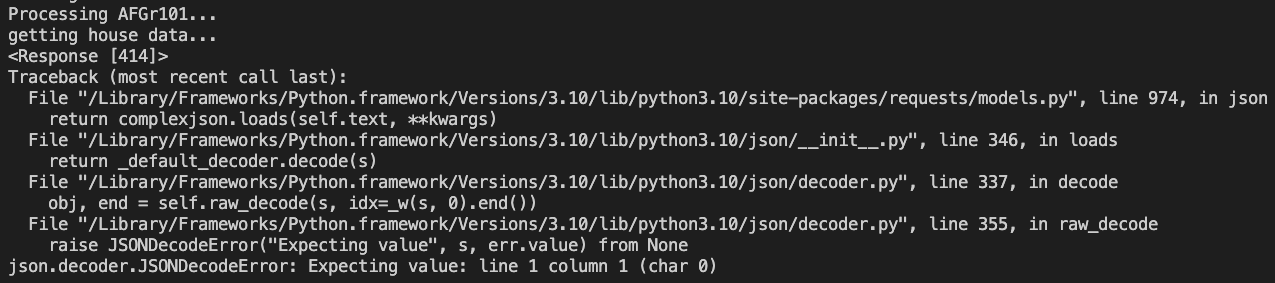
\includegraphics[width=15cm]{ss5.5.png}
\caption{HTTP \pil{414} Error}\label{fig:ss5.5}
\end{figure}

Unfortunately, this did not work and threw a HTTP \pil{414: URI Too Long} error, when trying to get the house data. As a result of this, the \pil{GET} request returned an empty string, and so the rest of the error message is a \pil{JSONDecodeError}, trying to decode an empty string into \pil{json}.

After researching the problem, I found that \pil{GET} requests have a maximum length, and going over it is considered ``abusing \pil{GET}''. I then went to the Overpass Turbo frontend, to test if my query works there, which it does. This lead me to believe that they aren't using a \pil{GET} request.

To find out what type of request they were using, I used the Safari Developer Tools, to see all of the incomming and outgoing traffic in the browser, including all HTTP requests.

\begin{figure}[H]
\centering
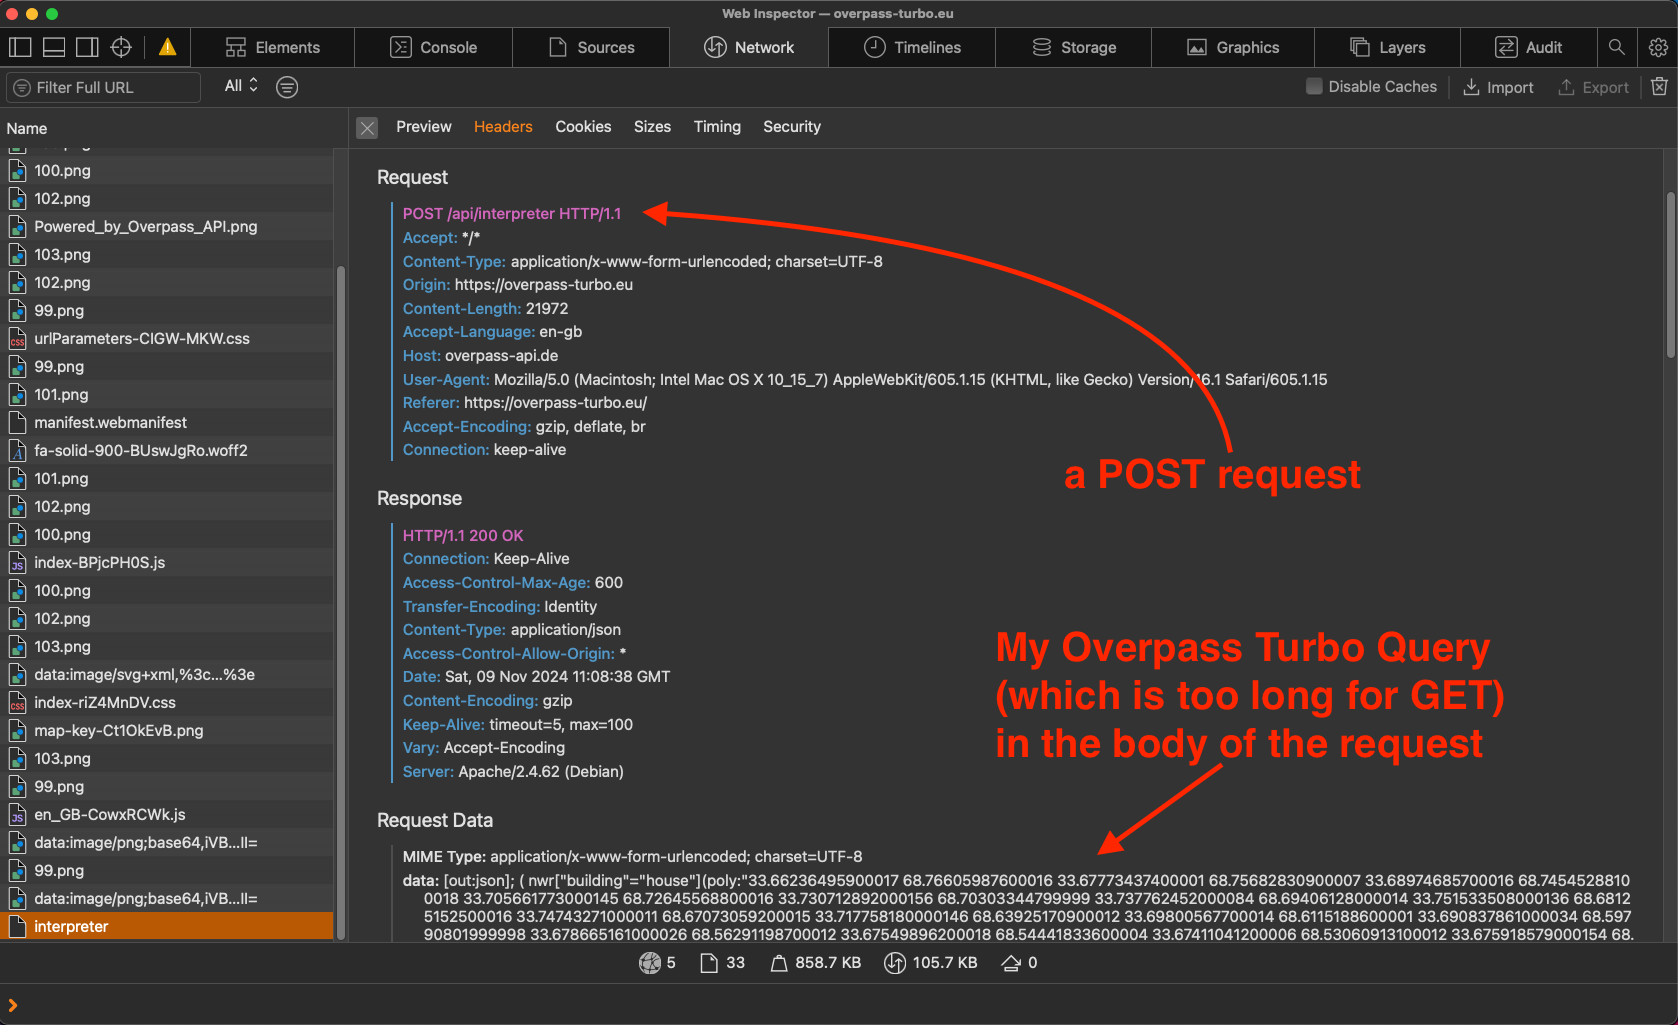
\includegraphics[width=14cm]{ss5.6.png}
\caption{Overpass Turbo's \pil{POST} request}\label{fig:ss5.6}
\end{figure}

It turns out that they are using a \pil{POST} request, and sending the Overpass Turbo query in the body of the request, instead of using a \pil{GET} request, and sending the query in the header.

\begin{listing}[H]
\pil{data_processing / get_osm_data.py / def get_osm_data}
\begin{minted}[linenos,breaklines,frame=single,firstnumber=17]{python}
    response = requests.post(overpass_url, data=overpass_query)
\end{minted}
\caption{Using a \pil{POST} request instead of a \pil{GET} request}\label{cs:postRequest}
\end{listing}

This code snippet replaces the original request, and implements the same thing that Overpass Turbo are doing on their frontend (using a \pil{POST} request and sending the query in the body of the request).

\begin{center}
\csvloop{
    file=data/minitests.csv,
    no head,
    column count=6,
    column names={1=\mtestID, 2=\mtestName, 3=\mtestInputs, 4=\mtestType, 5=\mtestExpectedOutputs, 6=\mtestRealOutputs},
    filter ifthen={\equal{\mtestID}{$t_{19}$}\AND\equal{\mtestInputs}{The AFGr101 region}\AND\equal{\mtestRealOutputs}{As Expected}\OR\equal{\mtestID}{\textbf{No.}}},
    before reading={
        \begin{longtable}{|m{1cm}|m{3cm}|m{3cm}|m{2cm}|m{3cm}|m{3cm}|}
        \hline
    },
    command=\csvlinetotablerow,
    late after line=\\\hline,
    after reading={
        \caption{Testing Table for Code Snippet \ref{cs:postRequest}}
        \end{longtable}
    }
}
\end{center}

\begin{figure}[H]
\centering
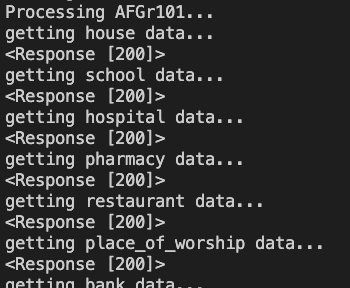
\includegraphics[width=9cm]{ss5.7.png}
\caption{All HTTP Responses now \pil{200: OK}}\label{fig:ss5.7}
\end{figure}

Unfortunately, by the time it reached the \nth{8} region (AFGr108), it came up with another error. This time, a HTTP \pil{400: Bad Request} error, which suggest that the format of my query is incorrect.

After looking into the problem, I found that the line to convert the \pil{list[coordinate]} (where \pil{coordinate} is a \pil{list[float]} or \pil{tuple[float]}) into a \pil{str} (which Overpass Turbo can read as a polygon) had not worked correctly, as each coordinate was still in a \pil{list}, rather than 2 numbers separated by a space. I then found that this region was stored as a \pil{list[list[list[coordinate]]]}, rather than a \pil{list[list[coordinate]]}.

\begin{figure}[H]
\centering
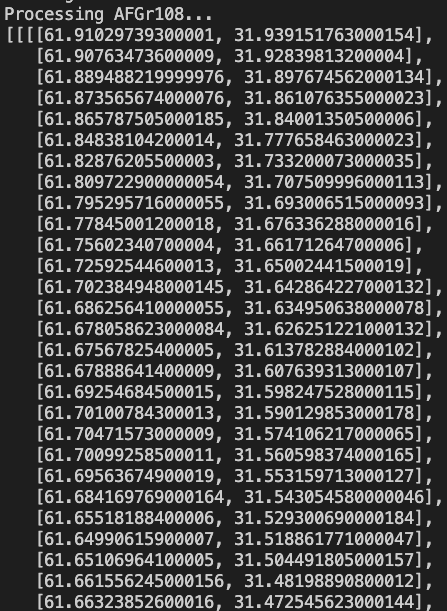
\includegraphics[width=8cm]{ss5.8.png}
\caption{\pil{list[list[list[coordinate]]]} debug print statement}\label{fig:ss5.8}
\end{figure}

Therefore, my initial assumption on how the regions must be stored is incorrect. After looking into the \pil{.geojson} documentation, I found that coordinates can be stored in 1 of 4 ways:
\begin{enumerate}
    \item \pil{'Coordinate'} (as \pil{coordinate}): A point on the Earth's Surface.
    \item \pil{'LineSegment'} (as \pil{list[coordinate]}): A set of \pil{'Coordinate'}s, joined together.
    \item \pil{'Polygon'} (as \pil{list[list[coordinate]]}): A set of \pil{'LineSegment'}s, to create a polygon.
    \item \pil{'MultiPolygon'} (as \pil{list[list[list[coordinate]]]}): A collection of \pil{'Polygon'}s.
\end{enumerate}
where \pil{coordinate} is a \pil{list[float]}. This means that regions AFGr101 to AFGr107 were of type \pil{'Polygon'}, but region AFGr108 is of type \pil{'MultiPolygon'}.

In my initial assumption, I had not accounted for the existance of the \pil{'LineSegment'}, which is why I was off by 1 dimension of \pil{list}s.

\begin{listing}[H]
\pil{data_processing / compile_data.py}
\begin{minted}[linenos,breaklines,frame=single,firstnumber=25]{python}
    # find the main bit of the region (if it has multiple)
    shapes = region['geometry']['coordinates']
    if region['geometry']['type'] == 'Polygon':
        mainShape = shapes[0]
    else:
        lengths = [len(polygon[0]) for polygon in shapes]
        mainShape = shapes[lengths.index(max(lengths))][0]
    mainShape = [coordinate[::-1] for coordinate in mainShape]
\end{minted}
\caption{Correctly finding the Main Area}\label{cs:findMainAreaAgain}
\end{listing}

Each region must either be a \pil{'Polygon'} or \pil{'MultiPolygon'}, with each \pil{'Polygon'} being 1 \pil{'LineSegment'}, as nothing else makes any sense.

If the region is a \pil{'Polygon'}, then it will just be a single \pil{'LineSegment'}, and so we can find it at the index \pil{0}.

Otherwise, it must be a \pil{'MultiPolygon'}, and so this is where we iterate over the lengths and find the main shape. We must also use the \pil{0} index here, to retrive the first (and only) \pil{'LineSegment'} from the \pil{'Polygon'}.

Afterwards, we must of course still reverse each coordinate, as they are still the wrong way around.

\begin{center}
\csvloop{
    file=data/minitests.csv,
    no head,
    column count=6,
    column names={1=\mtestID, 2=\mtestName, 3=\mtestInputs, 4=\mtestType, 5=\mtestExpectedOutputs, 6=\mtestRealOutputs},
    filter ifthen={\equal{\mtestID}{$t_{19}$}\AND\equal{\mtestInputs}{The AFGr108 region}\AND\equal{\mtestRealOutputs}{As Expected}\OR\equal{\mtestID}{\textbf{No.}}},
    before reading={
        \begin{longtable}{|m{1cm}|m{3cm}|m{3cm}|m{2cm}|m{3cm}|m{3cm}|}
        \hline
    },
    command=\csvlinetotablerow,
    late after line=\\\hline,
    after reading={
        \caption{Testing Table for Code Snippet \ref{cs:findMainAreaAgain}}
        \end{longtable}
    }
}
\end{center}

After doing this, I found that it was easier to specify the most recent region, instead of the number of regions done, when not starting from the beginning:

\begin{listing}[H]
\pil{data_processing / compile_data.py}
\begin{minted}[linenos,breaklines,frame=single,firstnumber=17]{python}
MOST_RECENT_REGION = 'AFGr108'
started = False
\end{minted}
\pil{data_processing / compile_data.py}
\begin{minted}[linenos,breaklines,frame=single,firstnumber=23]{python}
    if not started: 
        if region['properties']['gdlcode'] == MOST_RECENT_REGION:
            started = True
        continue
\end{minted}
\caption{Specifying the most recent region}\label{cs:specifyMostRecentRegion}
\end{listing}

\begin{center}
\csvloop{
    file=data/minitests.csv,
    no head,
    column count=6,
    column names={1=\mtestID, 2=\mtestName, 3=\mtestInputs, 4=\mtestType, 5=\mtestExpectedOutputs, 6=\mtestRealOutputs},
    filter ifthen={\equal{\mtestID}{$t_{16}$}\AND\equal{\mtestExpectedOutputs}{Starts on the next region}\OR\equal{\mtestID}{\textbf{No.}}},
    before reading={
        \begin{longtable}{|m{1cm}|m{3cm}|m{3cm}|m{2cm}|m{3cm}|m{3cm}|}
        \hline
    },
    command=\csvlinetotablerow,
    late after line=\\\hline,
    after reading={
        \caption{Testing Table for Code Snippet \ref{cs:specifyMostRecentRegion}}
        \end{longtable}
    }
}
\end{center}

Everything was downloading successfully until I got to Fiji, where it threw another HTTP \pil{400} error, which meant there was something wrong with my prompt again.

When pasting it into the Overpass Turbo frontend, it came back with an error, saying that I could not have coordinates whose longitude is greater that $180^{\circ}$, or less than $-180^{\circ}$. This makes sense as to why this error only came about when processing Fiji, as it almost lies on the international dateline.

\begin{figure}[H]
\centering
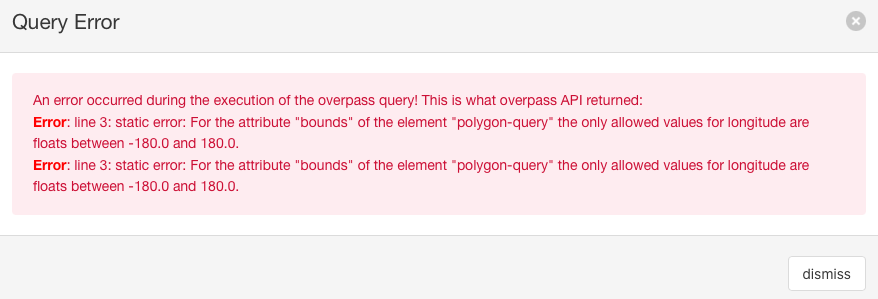
\includegraphics[width=14cm]{ss5.9.png}
\caption{Longitude Error Message}\label{fig:ss5.9}
\end{figure}

To fix this, we can add $180^{\circ}$ to it, and then mod $360^{\circ}$, and then subtract $180^{\circ}$ again, such that $-180^{\circ}\leq Lo\leq 180^{\circ}$. 

\begin{listing}[H]
\pil{data_processing / get_osm_data.py / def get_osm_data}
\begin{minted}[linenos,breaklines,frame=single,firstnumber=7]{python}
    bounding_coords = [(latitude, (longitude + 180) % 360 - 180) for latitude, longitude in bounding_coords]
\end{minted}
\caption{Finding the right Longitude}\label{cs:findRightLongitude}
\end{listing}

\begin{center}
\csvloop{
    file=data/minitests.csv,
    no head,
    column count=6,
    column names={1=\mtestID, 2=\mtestName, 3=\mtestInputs, 4=\mtestType, 5=\mtestExpectedOutputs, 6=\mtestRealOutputs},
    filter ifthen={\equal{\mtestID}{$t_{20}$}\OR\equal{\mtestID}{\textbf{No.}}},
    before reading={
        \begin{longtable}{|m{1cm}|m{3cm}|m{3cm}|m{2cm}|m{3cm}|m{3cm}|}
        \hline
    },
    command=\csvlinetotablerow,
    late after line=\\\hline,
    after reading={
        \caption{Testing Table for Code Snippet \ref{cs:findRightLongitude}}
        \end{longtable}
    }
}
\end{center}

Again, everything was downloading successfully, until this time Scotland caused a problem, throwing yet another HTTP \pil{400} error.

When I went to copy and paste the prompt into Overpass Turbo, in hopes of getting a similar error message, I quickly discovered that this prompt was much larger than the others, and had trouble copy and pasting it, as it was approximately 50 megabytes of text.

This was because Scotland was stored as a polygon with more than 500,000 vertices, most likely due to its irregular shape and jagged coastline, and so Overpass Turbo must have not been able to handle such a massive prompt.

Therefore, I decided to truncate regions with more than 100,000 vertices, by removing every other vertex until there were less than 100,000.

\begin{listing}[H]
\pil{data_processing / get_osm_data.py / def get_osm_data}
\begin{minted}[linenos,breaklines,frame=single,firstnumber=7]{python}
    while len(bounding_coords) >= 100000:
        print(f'truncating region with {len(bounding_coords)} vertices...') # log message
        bounding_coords = [bounding_coord for n, bounding_coord in enumerate(bounding_coords) if n % 2 == 0]
\end{minted}
\caption{Truncating Detailed Regions}\label{cs:truncatingRegions}
\end{listing}

\begin{center}
\csvloop{
    file=data/minitests.csv,
    no head,
    column count=6,
    column names={1=\mtestID, 2=\mtestName, 3=\mtestInputs, 4=\mtestType, 5=\mtestExpectedOutputs, 6=\mtestRealOutputs},
    filter ifthen={\equal{\mtestID}{$t_{21}$}\OR\equal{\mtestID}{\textbf{No.}}},
    before reading={
        \begin{longtable}{|m{1cm}|m{3cm}|m{3cm}|m{2cm}|m{3cm}|m{3cm}|}
        \hline
    },
    command=\csvlinetotablerow,
    late after line=\\\hline,
    after reading={
        \caption{Testing Table for Code Snippet \ref{cs:truncatingRegions}}
        \end{longtable}
    }
}
\end{center}

The rest of the process went smoothly, with no other errors, except for the occasional time out.

\begin{figure}[H]
\centering
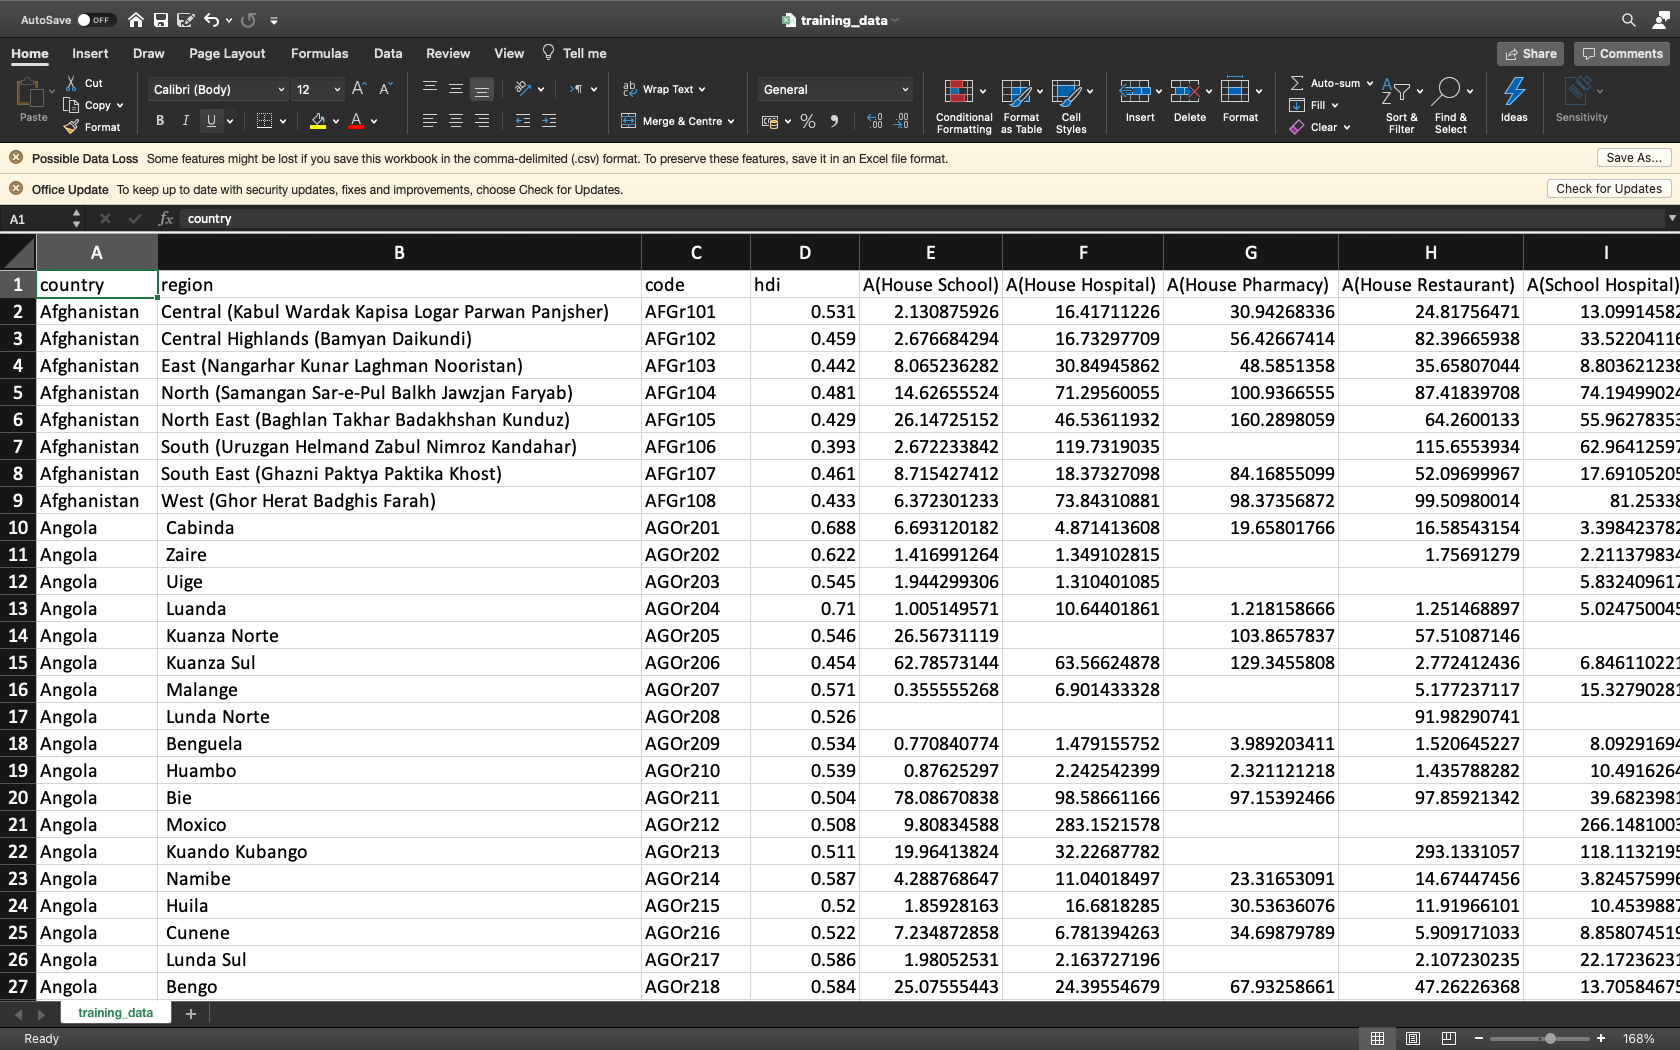
\includegraphics[width=12cm]{ss5.10.png}
\caption{Final Training Data}\label{fig:ss5.10}
\end{figure}

Figure \ref{fig:ss5.10} shows the final \pil{.csv} file, containing the training data for the neural network, which is what I had hoped to have achieved by the end of this milestone.

I can now therefore delete \pil{region_coords.json} and \pil{hdi.csv}, as I only needed them to create \pil{training_data.csv}.

\subsection{Review}

\begin{center}
\csvloop{
    file=data/testdata.csv,
    no head,
    column count=5,
    column names={1=\testID, 2=\testName, 3=\testInputs, 4=\testOutputs, 5=\testSuccess},
    filter ifthen={\equal{\testID}{$T_{1}$}\OR\equal{\testID}{$T_{2}$}\OR\equal{\testID}{$T_{3}$}\OR\equal{\testID}{$T_{4}$}\OR\equal{\testID}{\textbf{No.}}},
    before reading={
        \begin{longtable}{|m{1cm}|m{3cm}|m{8cm}|H|m{2cm}|}
        \hline
    },
    command=\csvlinetotablerow,
    late after line=\\\hline,
    after reading={
        \caption{Passed Testing Data for Milestone 1}
        \end{longtable}
    }
}
\end{center}

After some successful debugging, all 4 of the main tests in Milestone 1 passed. As a result of that, the following success criteria has been met:

\begin{center}
\csvloop{
    file=data/successcriteria.csv,
    no head,
    column count=5,
    column names={1=\scID, 2=\scCriterion, 3=\scJustification, 4=\scSuccess, 5=\scEvaluation},
    filter ifthen={\equal{\scID}{$S_{1}$}\OR\equal{\scID}{$S_{2}$}\OR\equal{\scID}{$S_{3}$}\OR\equal{\scID}{$S_{4}$}\OR\equal{\scID}{\textbf{No.}}},
    before reading={
        \begin{longtable}{|m{1cm}|m{5cm}|m{6cm}|m{2cm}|H}
        \hline
    },
    command=\csvlinetotablerow,
    late after line=\\\hline,
    after reading={
        \caption{Achieved Success Criteria for Milestone 1}
        \end{longtable}
    }
}
\end{center}

I also have a full set of training data, so overall, I believe this milestone has been a success.

\section{Milestone 2 -- Multilayer Perceptron}
\subsection{Success Criteria}
By the end of this milestone, I hope to have a fully trained neural network, which is able of predicting HDI from a set of factors.
\begin{center}
\csvloop{
    file=data/successcriteria.csv,
    no head,
    column count=5,
    column names={1=\scID, 2=\scCriterion, 3=\scJustification, 4=\scSuccess, 5=\scEvaluation},
    filter ifthen={\equal{\scID}{$S_{5}$}\OR\equal{\scID}{$S_{6}$}\OR\equal{\scID}{$S_{7}$}\OR\equal{\scID}{\textbf{No.}}},
    before reading={
        \begin{longtable}{|m{1cm}|m{5cm}|m{8cm}|H H}
        \hline
    },
    command=\csvlinetotablerow,
    late after line=\\\hline,
    after reading={
        \caption{Success Criteria for Milestone 2}
        \end{longtable}
    }
}
\end{center}

To determine if I have met this success criteria, I will be using the following test:

\begin{center}
\csvloop{
    file=data/testdata.csv,
    no head,
    column count=5,
    column names={1=\testID, 2=\testName, 3=\testInputs, 4=\testOutputs, 5=\testSuccess},
    filter ifthen={\equal{\testID}{$T_{5}$}\OR\equal{\testID}{\textbf{No.}}},
    before reading={
        \begin{longtable}{|m{1cm}|m{3cm}|m{5cm}|m{5cm}|H}
        \hline
    },
    command=\csvlinetotablerow,
    late after line=\\\hline,
    after reading={
        \caption{Testing Data for Milestone 2}
        \end{longtable}
    }
}
\end{center}

Again, determining if the neural network is actually working is very difficult, so I indtend to train a neural network to do something else, like recognise handwritten digits, which certainly has enough training data, to determine if it is working in principle.

\stepcounter{parts}
\subsection{Part \theparts{} -- Implementing the Neural Network Structure}

We must first define the constructor method for a Multilayer Pereptron.

\begin{listing}[H]
\pil{neural_network.py}
\begin{minted}[linenos,breaklines,frame=single,firstnumber=1]{python}
import numpy as np

class MultilayerPerceptron(object):
    # constructor method
    def __init__(self, layer_sizes):
        # initialise layer sizes constant
        self.layer_sizes = layer_sizes
        self.L = len(layer_sizes)-1
\end{minted}
\caption{Defining the Constructor Method}\label{cs:definingConstructor}
\end{listing}

Here, I am importing \pil{numpy}, as it will be very useful in all the calculations we will be doing in this class.

Next, we define the \pil{class MultilayerPerceptron}, which inherits from the generic python \pil{object}. As stated before, we must only pass the \pil{layer_sizes} into the constructor method (as well as \pil{self}), as everything else can be defined implicitly from that.

The \pil{layer_sizes} attribute will obviously be set to the \pil{layer_sizes} parameter, and the \pil{L} attribute is the number of layers, not including the input layer, so we subtract 1 from the length of the \pil{layer_sizes} \pil{list}.

\begin{listing}[H]
\pil{neural_network.py / class MultilayerPerceptron / def __init__}
\begin{minted}[linenos,breaklines,frame=single,firstnumber=9]{python}
        # initialise matrices for the different quantities
        self.activations = [np.matrix(np.zeros(shape=(layer_size,1))) for layer_size in layer_sizes]
        self.weights = [np.matrix(np.random.randn(layer_sizes[index+1],layer_size)) for index, layer_size in enumerate(layer_sizes[:-1])]
        self.biases = [np.matrix(np.random.randn(layer_size,1)) for layer_size in layer_sizes]
        self.z = [np.matrix(np.zeros(shape=(layer_size,1))) for layer_size in layer_sizes]
        self.errors = [np.matrix(np.zeros(shape=(layer_size,1))) for layer_size in layer_sizes]
\end{minted}
\caption{Initialising the Matrices}\label{cs:initialisingMatrices}
\end{listing}

Next, I added the attributes of all the \pil{list}s of matrices, and column vectors, representing the activations, weights, biases, $z$-values and errors within the network.

The activations of the neurons are stored as a \pil{list} of column vectors, where the size of each column vector is that layer's size. The activations will initially be set to 0, so we can use the \pil{np.zeros} function to get a multidimensional array of 0s. The size of multidimensional array we want is \pil{layer_size} rows and 1 column, for some \pil{layer_size}. To turn this into a column vector, we pass this into the \pil{np.matrix} function, as done before. To get the full \pil{list}, we must iterate this process for each of the \pil{layer_size}s in \pil{layer_sizes}. The \pil{z} and \pil{errors} attributes are set to the same lists, as they are also quantities stored in neurons and should also be 0s to begin with.

Bias is also a quantity stored in the neurons, but should not be set to 0 to begin with, as it is a parameter of the system. Instead it should be set to a random number, which has been picked from a random distribution. To get a sensible range of values, I used the standard normal distribution (using \pil{np.random.randn} in place of \pil{np.zeros}):

\begin{figure}[H]
\centering
\begin{tikzpicture}
\begin{axis}[
    axis lines=middle,
    axis line style={-stealth,shorten >=-3mm},
    ymax=0.5,
    xlabel = $x$,
    ylabel = Probability Density,
    width=\columnwidth,
    height=2in,
    scale only axis
]
\addplot[
    domain=-4:4,
    samples=100,
    red
]{e^(-(1/2)*(x^2))/sqrt(2*pi)};
\end{axis}
\end{tikzpicture}
\caption{Graph of the Standard Normal Distribution}\label{fig:normalDistribution}
\end{figure}

Figure \ref{fig:normalDistribution} visually shows the normal distribution, and its bell-shaped curve. Most of the random values should therefore be in between $-2$ and 2, with very few being outside that range.

Weights are also paramaters of the system, and so should also get random values from the normal distribution. However, weights should be stored as a matrix between 2 layers, and so the shape must be different. Here, the number of rows must be the size of the next layer (\pil{layer_sizes[index+1]}), and the number of columns must be the size of the current layer (\pil{layer_size}). This time, instead of iterating over all of the layer sizes, we must only go up to 1 before the end, again due to the fact that weights go in between the layers.

\begin{figure}[H]
\centering
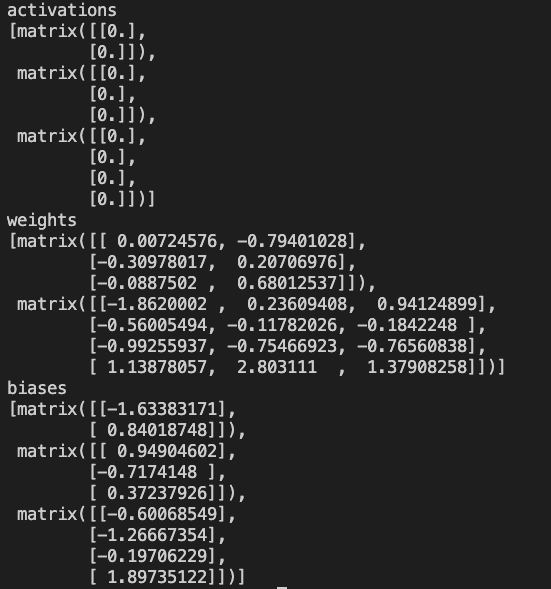
\includegraphics[width=10cm]{ss6.1.png}
\caption{Printing activations, weights and biases}\label{fig:ss6.1}
\end{figure}

Figure \ref{fig:ss6.1} shows the output if we print \pil{self.activations}, \pil{self.weights} and \pil{self.biases}, for a neural network with \pil{layer_sizes = [2,3,4]} (\pil{self.z} and \pil{self.errors} will be the same as \pil{self.activations}).

The final attributes we must define are the copies of the activations, $z$-values and errors used in training.

\begin{listing}[H]
\pil{neural_network.py}
\begin{minted}[linenos,breaklines,frame=single,firstnumber=2]{python}
import copy
\end{minted}
\pil{neural_network.py / class MultilayerPerceptron / def __init__}
\begin{minted}[linenos,breaklines,frame=single,firstnumber=16]{python}
        # initialise lists for training states
        self.training_activations = []
        self.training_z = []
        self.training_errors = []
\end{minted}
\caption{Initialising the Training Lists}\label{cs:initialisingTrainingLists}
\end{listing}

Right now, they are set as empty lists, as we have not done any training yet.

In anticipation of making copies of the attributes, I have also imported the \pil{copy} library.

\begin{center}
\csvloop{
    file=data/minitests.csv,
    no head,
    column count=6,
    column names={1=\mtestID, 2=\mtestName, 3=\mtestInputs, 4=\mtestType, 5=\mtestExpectedOutputs, 6=\mtestRealOutputs},
    filter ifthen={\equal{\mtestID}{$t_{22}$}\OR\equal{\mtestID}{$t_{23}$}\OR\equal{\mtestID}{$t_{24}$}\OR\equal{\mtestID}{$t_{25}$}\OR\equal{\mtestID}{\textbf{No.}}},
    before reading={
        \begin{longtable}{|m{1cm}|m{3cm}|m{3cm}|m{2cm}|m{3cm}|m{3cm}|}
        \hline
    },
    command=\csvlinetotablerow,
    late after line=\\\hline,
    after reading={
        \caption{Testing Table for Code Snippets \ref{cs:definingConstructor}, \ref{cs:initialisingMatrices} \& \ref{cs:initialisingTrainingLists}}
        \end{longtable}
    }
}
\end{center}

We must also define the sigmoid function, to use as our activation function.

\begin{listing}[H]
\pil{neural_network.py}
\begin{minted}[linenos,breaklines,frame=single,firstnumber=21]{python}
# activation function
def sigmoid(x):
    return 1/(1+np.exp(-x))
\end{minted}
\caption{Defining the Sigmoid Function}\label{cs:sigmoidFunction}
\end{listing}

This matches with the definition stated in equation \ref{eq:sigmoid}. In the class diagram (Figure \ref{fig:classDiagram}), I had made this function a method in the \pil{class MultilayerPerceptron}, but now I believe that it makes more sense for it to be a stand-alone function, as it does not use any of the attributes from the class.

We must also define the derivative of the sigmoid function, as it will be used in the backpropogation algorithm. We can differentiate it using the quotient rule, and then rearrange it so that it is in terms of $\sigma\left(x\right)$:

\begin{equation}\label{eq:sigmoidDerivative}
\begin{split}
    {\sigma}^{\prime} \left(x\right)&=\diff{}{x}\left(\frac{1}{1+e^{-x}}\right) \\
    &=\frac{\left(0\right)\left(1+e^{-x}\right)-\left(1\right)\left(-e^{-x}\right)}{{\left(1+e^{-x}\right)}^2} \\
    &=\frac{e^{-x}}{{\left(1+e^{-x}\right)}^2} \\
    &=\left(\frac{e^{-x}}{1+e^{-x}}\right)\left(\frac{1}{1+e^{-x}}\right) \\
    &=\left(\frac{1+e^{-x}-1}{1+e^{-x}}\right)\left(\frac{1}{1+e^{-x}}\right) \\
    &=\left(\frac{1+e^{-x}}{1+e^{-x}}-\frac{1}{1+e^{-x}}\right)\left(\frac{1}{1+e^{-x}}\right) \\
    &=\left(1-\sigma\left(x\right)\right)\left(\sigma\left(x\right)\right)
\end{split}
\end{equation}

\begin{listing}[H]
\pil{neural_network.py}
\begin{minted}[linenos,breaklines,frame=single,firstnumber=25]{python}
# derivative of the activation function
def sigmoid_prime(x):
    return sigmoid(x)*(1-sigmoid(x))
\end{minted}
\caption{Defining the derivative of the Sigmoid Function}\label{cs:sigmoidPrimeFunction}
\end{listing}

Again, this was previously planned to be a method in the \pil{class MultilayerPerceptron}, but I have since decided to move it out.

\begin{center}
\csvloop{
    file=data/minitests.csv,
    no head,
    column count=6,
    column names={1=\mtestID, 2=\mtestName, 3=\mtestInputs, 4=\mtestType, 5=\mtestExpectedOutputs, 6=\mtestRealOutputs},
    filter ifthen={\equal{\mtestID}{$t_{26}$}\OR\equal{\mtestID}{$t_{27}$}\OR\equal{\mtestID}{\textbf{No.}}},
    before reading={
        \begin{longtable}{|m{1cm}|m{3cm}|m{3cm}|m{2cm}|m{3cm}|m{3cm}|}
        \hline
    },
    command=\csvlinetotablerow,
    late after line=\\\hline,
    after reading={
        \caption{Testing Table for Code Snippets \ref{cs:sigmoidFunction} \& \ref{cs:sigmoidPrimeFunction}}
        \end{longtable}
    }
}
\end{center}

We must also create methods for saving and loading weights and biases.

\begin{listing}[H]
\pil{neural_network.py}
\begin{minted}[linenos,breaklines,frame=single,firstnumber=3]{python}
import pickle
\end{minted}
\pil{neural_network.py / class MultilayerPerceptron}
\begin{minted}[linenos,breaklines,frame=single,firstnumber=22]{python}
    # saves weights and biases to an external file in the models folder
    def save_model(self, filename):
        parameters = {
            'weights': self.weights,
            'biases': self.biases
        }
        with open(f'models/{filename}.pkl', 'wb') as file:
            pickle.dump(parameters, file)
\end{minted}
\caption{Saving weights and biases}\label{cs:savingModels}
\end{listing}

As stated before, we can save the weights and biases attributes to a python \pil{dict}, and then write that dictionary to a file. I believe the most suitable file type is the \pil{.pkl} binary file, which can be use to store variables. As this is a binary file, we must open it in \pil{'wb'} mode (w for write, b for binary), and then dump the \pil{parameters} dictionary using the \pil{pickle} module (which we must import first).

\begin{listing}[H]
\pil{neural_network.py / class MultilayerPerceptron}
\begin{minted}[linenos,breaklines,frame=single,firstnumber=31]{python}
    # loads a model from a file path
    def load_model(self, file_path):
        with open(file_path, 'rb') as file:
            parameters = pickle.load(file)
        self.weights = parameters['weights']
        self.biases = parameters['biases']
\end{minted}
\caption{Loading Models}\label{cs:loadingModels}
\end{listing}

To load the model, we can do the same thing but in reverse. First, open the file in \pil{'rb'} mode (r for read, b for binary) and load the dictionary into a \pil{parameters} variable. We can then set the \pil{weights} and \pil{biases} attributes to the respective elements in the dictionary.

\begin{center}
\csvloop{
    file=data/minitests.csv,
    no head,
    column count=6,
    column names={1=\mtestID, 2=\mtestName, 3=\mtestInputs, 4=\mtestType, 5=\mtestExpectedOutputs, 6=\mtestRealOutputs},
    filter ifthen={\equal{\mtestID}{$t_{28}$}\OR\equal{\mtestID}{$t_{29}$}\OR\equal{\mtestID}{\textbf{No.}}},
    before reading={
        \begin{table}[H]
        \centering
        \begin{tabular}{|m{1cm}|m{3cm}|m{3cm}|m{2cm}|m{3cm}|m{3cm}|}
        \hline
    },
    command=\csvlinetotablerow,
    late after line=\\\hline,
    after reading={
        \end{tabular}
        \caption{Testing Table for Code Snippets \ref{cs:savingModels} \& \ref{cs:loadingModels}}
        \end{table}
    }
}
\end{center}

We should only be able to load weights and biases if they originally came from a network with the same layer sizes.

\begin{listing}[H]
\pil{neural_network.py / class MultilayerPerceptron / def save_model}
\begin{minted}[linenos,breaklines,frame=single,firstnumber=24]{python}
        parameters = {
            'weights': self.weights,
            'biases': self.biases,
            'layer_sizes': self.layer_sizes
        }
\end{minted}
\pil{neural_network.py / class MultilayerPerceptron / def load_model}
\begin{minted}[linenos,breaklines,frame=single,firstnumber=36]{python}
        if self.layer_sizes != parameters['layer_sizes']:
            raise Exception('layer sizes do not match!')
\end{minted}
\caption{Ensuring Layer Sizes are the Same}\label{cs:sameLayerSizes}
\end{listing}

To do this, we can also store the \pil{layer_sizes} attribute in the dictionary which is written to file, and then when loading, we can check if the \pil{layer_sizes} in the dictionary matches this instance's \pil{layer_sizes}, before we set the weights and biases. If it does not match, then we can \pil{raise} an \pil{Exception}, to say that the layer sizes do not match.

\begin{center}
\csvloop{
    file=data/minitests.csv,
    no head,
    column count=6,
    column names={1=\mtestID, 2=\mtestName, 3=\mtestInputs, 4=\mtestType, 5=\mtestExpectedOutputs, 6=\mtestRealOutputs},
    filter ifthen={\equal{\mtestID}{$t_{30}$}\OR\equal{\mtestID}{\textbf{No.}}},
    before reading={
        \begin{longtable}{|m{1cm}|m{3cm}|m{3cm}|m{2cm}|m{3cm}|m{3cm}|}
        \hline
    },
    command=\csvlinetotablerow,
    late after line=\\\hline,
    after reading={
        \caption{Testing Table for Code Snippet \ref{cs:sameLayerSizes}}
        \end{longtable}
    }
}
\end{center}

\stepcounter{parts}
\subsection{Part \theparts{} -- Implementing the Feedforward Algorithm \& Prediction}

Now it's time to implement the Feedforward algorithm, as shown in the flowchart in Figure \ref{fig:feedforward}.

\begin{listing}[H]
\pil{neural_network.py / class MultilayerPerceptron}
\begin{minted}[linenos,breaklines,frame=single,firstnumber=22]{python}
    # carry out the feedforward algorithm
    def feedforward(self):
        for layer in range(0, self.L):
            self.z[layer+1] = np.matmul(self.weights[layer], self.activations[layer]) + self.biases[layer+1]
            self.activations[layer+1] = sigmoid(self.z[layer+1])
\end{minted}
\caption{Implementing the Feedforward Algorithm}\label{cs:feedforwardAlgo}
\end{listing}

In the flowchart and the class diagam, I had said the input layer would be an input/parameter to this function, but I have since decided it would make more sense to just directly access it from the \pil{self.activations} attribute (it will be at index \pil{0}).

Next, according to the flowchart, we must iterate for $l$ from 0 to $L-1$, which can be simply done with a python \pil{for} loop (iterator variable renamed to \pil{layer} for greater readability).

Then for each of the values for $l$ (\pil{layer}), we must compute $\mathbf{a}^{\left(l+1\right)}=\sigma \left(\mathbf{W}^{\left(l\right)}\mathbf{a}^{\left(l\right)}+\mathbf{b}^{\left(l+1\right)}\right)$ (equation \ref{eq:activationOfLayer}). As we will also need to get the various values for $z$ during training, I have broken this expression up into $\mathbf{z}^{\left(l+1\right)}=\mathbf{W}^{\left(l\right)}\mathbf{a}^{\left(l\right)}+\mathbf{b}^{\left(l+1\right)}$ and $\mathbf{a}^{\left(l+1\right)}=\sigma \left(\mathbf{z}^{\left(l+1\right)}\right)$, which you can see implemented on lines 25 and 26.

\begin{listing}[H]
\pil{neural_network.py / class MultilayerPerceptron}
\begin{minted}[linenos,breaklines,frame=single,firstnumber=28]{python}
    # run the feedforward algorithm on a set of input data and return the result
    def predict(self, input_data):
        self.activations[0] = input_data
        self.feedforward()
        return self.activations[self.L]
\end{minted}
\caption{Making a Prediction}\label{cs:predictionWrapper}
\end{listing}

If we then want to more formally make a prediction, we must first get the input data (the parameter of this \pil{def predict} function), then feed it forward through the network, and return the activations in the output layer (the layer at index $L$).

\begin{center}
\csvloop{
    file=data/minitests.csv,
    no head,
    column count=6,
    column names={1=\mtestID, 2=\mtestName, 3=\mtestInputs, 4=\mtestType, 5=\mtestExpectedOutputs, 6=\mtestRealOutputs},
    filter ifthen={\equal{\mtestID}{$t_{31}$}\OR\equal{\mtestID}{$t_{32}$}\OR\equal{\mtestID}{\textbf{No.}}},
    before reading={
        \begin{table}[H]
        \centering
        \begin{tabular}{|m{1cm}|m{3cm}|m{3cm}|m{2cm}|m{3cm}|m{3cm}|}
        \hline
    },
    command=\csvlinetotablerow,
    late after line=\\\hline,
    after reading={
        \end{tabular}
        \caption{Testing Table for Code Snippets \ref{cs:feedforwardAlgo} \& \ref{cs:predictionWrapper}}
        \end{table}
    }
}
\end{center}

Again, due to the nature of the caulculations involved in the network, it is difficult to test these algorithms. Therefore, I was only looking for the correct structure of the answers (e.g. the correct dimensions of matrix) to determine if the output is as expected.

\stepcounter{parts}
\subsection{Part \theparts{} -- Implementing the Backpropogation Algorithm \& Training}

If we actually try to make a prediction, the network will return absolute nonsense, and so we must be able to train it, using the backpropogation algorithm.

\begin{listing}[H]
\pil{neural_network.py / class MultilayerPerceptron}
\begin{minted}[linenos,breaklines,frame=single,firstnumber=28]{python}
    # carry out the backpropogation algorithm
    def backpropogate(self, examples):
        # reset the training lists
        # iterate over each example
        for example in examples:
            # reset the activations, z-values and errors
            # make a feedforward pass
            # calculate the error in the output layer
            # backpropogate the error to previous layers
            # save the activations, z-values and errors
        # use gradient descent to update the weights and biases
\end{minted}
\caption{Backpropogation Algorithm Structure}\label{cs:backpropogationShell}
\end{listing}

Here, in Code Snippet \ref{cs:backpropogationShell}, I have outlined the general backpropogation algorithm, as shown in the flowchart in Figure \ref{fig:backpropogation}, with some additional steps we need to consider when practically carrying it out (for example, resetting the lists).

\begin{listing}[H]
\pil{neural_network.py / class MultilayerPerceptron / def backpropogate}
\begin{minted}[linenos,breaklines,frame=single,firstnumber=30]{python}
        # reset the training lists
        self.training_activations = []
        self.training_z = []
        self.training_errors = []
        # iterate over each example
        for example in examples:
            # reset the activations, z-values and errors
            self.activations = [np.matrix(np.zeros(shape=(layer_size,1))) for layer_size in self.layer_sizes]
            self.z = [np.matrix(np.zeros(shape=(layer_size,1))) for layer_size in self.layer_sizes]
            self.errors = [np.matrix(np.zeros(shape=(layer_size,1))) for layer_size in self.layer_sizes]
\end{minted}
\caption{Resetting the Lists}\label{cs:backpropogationResetLists}
\end{listing}

Resetting these lists is easy enough, as all we need to do is ensure the training lists are empty, and reset the activations, $z$-values and errors to 0 when processing each example (by doing the same things as in the constructor method).

\begin{listing}[H]
\pil{neural_network.py / class MultilayerPerceptron / def backpropogate}
\begin{minted}[linenos,breaklines,frame=single,firstnumber=40]{python}
            # make a feedforward pass
            self.activations[0] = example['input']
            self.feedforward()
            # calculate the error in the output layer
            self.errors[self.L] = np.multiply(
                self.activations[self.L] - example['output'],
                sigmoid_prime(self.z[self.L])
            )
\end{minted}
\caption{Calculating the error in the output layer}\label{cs:backpropogationOutputLayer}
\end{listing}

Next, we must feedforward the example's input, to get the network's current prediction, and then compare that with the ``correct'' output to get the error.

We must use the formula $\bm{\delta}^{\left(L\right)}=\left(\mathbf{a}^{\left(L\right)}-\mathbf{y}\right)\odot \left({\sigma}^{\prime} \left(\mathbf{z}^{\left(L\right)}\right)\right)$ (equation \ref{eq:errorOutputLayer}) to calculate the error in the output layer, which has been implemented in lines 44 to 47 (the \pil{np.multiply} function carries out the $\odot$ operation). 

\begin{listing}[H]
\pil{neural_network.py / class MultilayerPerceptron / def backpropogate}
\begin{minted}[linenos,breaklines,frame=single,firstnumber=48]{python}
            # backpropogate the error to previous layers
            for layer in range(self.L, 1, -1):
                self.errors[layer-1] = np.multiply(
                    np.matmul(
                        self.weights[layer-1].T,
                        self.errors[layer]
                    ),
                    sigmoid_prime(self.z[layer-1])
                )
            # save the activations, z-values and errors
            self.training_activations.append( copy.deepcopy(self.activations))
            self.training_z.append(copy.deepcopy(self.z))
            self.training_errors.append(copy.deepcopy(self.errors))
\end{minted}
\caption{Backpropogating the Error}\label{cs:backpropogationBackpropogation}
\end{listing}

After this, we can backpropogate the error, using the formula $\bm{\delta}^{\left(l-1\right)}=\left({\left(\mathbf{W}^{\left(l-1\right)}\right)}^{T}\bm{\delta}^{\left(l\right)}\right)\odot\left({\sigma}^{\prime} \left(\mathbf{z}^{\left(l-1\right)}\right)\right)$ (equation \ref{eq:backpropogateError}), for each $l$ from $L$ to 2. The iteration is easily implemented with a \pil{for} loop on line 49, and the equation is implemented in lines 50 to 56. The attribute \pil{.T} of a \pil{np.matrix} is the transpose of that matrix, as required by the formula.

Now that we have a full set of activations, $z$-values, and errors, we can save them to their respective lists to be able to compute the gradient of the cost function.

\begin{listing}[H]
\pil{neural_network.py / class MultilayerPerceptron}
\begin{minted}[linenos,breaklines,frame=single,firstnumber=29]{python}
    def backpropogate(self, examples, learning_rate):
\end{minted}
\pil{neural_network.py / class MultilayerPerceptron / def backpropogate}
\begin{minted}[linenos,breaklines,frame=single,firstnumber=61]{python}
        # use gradient descent to update the weights and biases
        for layer in range(self.L, 0, -1):
            self.weights[layer-1] -= (learning_rate/len(examples)) * sum(
                [np.matmul(
                    self.training_errors[example][layer],
                    self.training_activations[example][layer-1].T
                ) for example in range(len(examples))],
                np.matrix(np.zeros(self.weights[layer-1].shape)) # (extra argument in sum function to add matrices instead of numbers)
            )
            self.biases[layer] -= (learning_rate/len(examples)) * sum(
                [self.training_errors[example][layer] for example in range(len(examples))],
                np.matrix(np.zeros(self.biases[layer].shape)) # (extra argument in sum function to add matrices instead of numbers)
            )
\end{minted}
\caption{Updating the weights and biases}\label{cs:backpropogationGradientDescent}
\end{listing}

Finally, we must update the weights using the formula $\mathbf{W}^{\left(l-1\right)}=\mathbf{W}^{\left(l-1\right)}-\frac{\eta}{m}\displaystyle\sum_{x=1}^{m}\bm{\delta}^{\left(l\right)}_x{\left(\mathbf{a}^{\left(l-1\right)}_x\right)}^T$ (equation \ref{eq:updateWeights}), implemented on lines 63 to 69.

And we must update the biases using the formula $\mathbf{b}^{\left(l\right)}=\mathbf{b}^{\left(l\right)}-\frac{\eta}{m}\displaystyle\sum_{x=1}^{m}\bm{\delta}^{\left(l\right)}_x$ (equation \ref{eq:updateBiases}), implemented on lines 70 to 73. (for each of the layers from the final layer, to the input layer).

One of the terms in these equations is $\eta$, the learning rate, which is just a constant to determine how fast the network should learn. I had forgotten to add this as a parameter of the \pil{def backpropogate} function in the class diagram, but I have since added it here.

Both of these formulas also involve summing over multiple matrices, which I have implemented with the default python \pil{sum} function. As we are summing matrices instead of numbers, we must also pass in a matrix of 0s, of the same dimension as the matrix we are updating, for the sum to work.

This should be the full backpropogation algorithm, and so we are ready to test it. All I am looking for at the moment is that it does not throw an error, as it is impossible to determine if the answer is correct or not without carrying out the algorithm again.

\begin{center}
\csvloop{
    file=data/minitests.csv,
    no head,
    column count=6,
    column names={1=\mtestID, 2=\mtestName, 3=\mtestInputs, 4=\mtestType, 5=\mtestExpectedOutputs, 6=\mtestRealOutputs},
    filter ifthen={\equal{\mtestID}{$t_{33}$}\AND\equal{\mtestRealOutputs}{An Error}\OR\equal{\mtestID}{\textbf{No.}}},
    before reading={
        \begin{longtable}{|m{1cm}|m{3cm}|m{3cm}|m{2cm}|m{3cm}|m{3cm}|}
        \hline
    },
    command=\csvlinetotablerow,
    late after line=\\\hline,
    after reading={
        \caption{Testing Table for Code Snippets \ref{cs:backpropogationShell}, \ref{cs:backpropogationResetLists}, \ref{cs:backpropogationOutputLayer}, \ref{cs:backpropogationBackpropogation} \& \ref{cs:backpropogationGradientDescent}}
        \end{longtable}
    }
}
\end{center}

\begin{figure}[H]
\centering
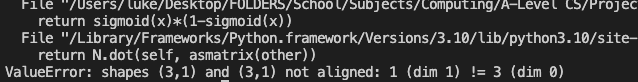
\includegraphics[width=14cm]{ss8.1.png}
\caption{Backpropogation Error}\label{fig:ss8.1}
\end{figure}

The error seems to be that we are attempty to carry out matrix multiplication between $\sigma\left(x\right)$ and $1-\sigma\left(x\right)$.

\begin{listing}[H]
\pil{neural_network.py}
\begin{minted}[linenos,breaklines,frame=single,firstnumber=100]{python}
# derivative of the activation function
def sigmoid_prime(x):
    return np.multiply(sigmoid(x), 1-sigmoid(x))
\end{minted}
\caption{Fixing the ${\sigma}^{\prime}$ function}\label{cs:fixSigmoidPrime}
\end{listing}

We can fix this by specifying we want to do an element-wise multiplication \pil{np.multiply} instead of a matrix multiplication.

\begin{center}
\csvloop{
    file=data/minitests.csv,
    no head,
    column count=6,
    column names={1=\mtestID, 2=\mtestName, 3=\mtestInputs, 4=\mtestType, 5=\mtestExpectedOutputs, 6=\mtestRealOutputs},
    filter ifthen={\equal{\mtestID}{$t_{33}$}\AND\equal{\mtestRealOutputs}{As Expected}\OR\equal{\mtestID}{\textbf{No.}}},
    before reading={
        \begin{longtable}{|m{1cm}|m{3cm}|m{3cm}|m{2cm}|m{3cm}|m{3cm}|}
        \hline
    },
    command=\csvlinetotablerow,
    late after line=\\\hline,
    after reading={
        \caption{Testing Table for Code Snippet \ref{cs:fixSigmoidPrime}}
        \end{longtable}
    }
}
\end{center}

The backpropogation algorithm now does not crash. Whether or not it actually works will be tested shortly, in the next section.

\begin{listing}[H]
\pil{neural_network.py}
\begin{minted}[linenos,breaklines,frame=single,firstnumber=4]{python}
import random
\end{minted}
\pil{neural_network.py / class MultilayerPerceptron}
\begin{minted}[linenos,breaklines,frame=single,firstnumber=82]{python}
    # carry out stochastic gradient descent over a number of epochs to train a model
    def train(self, examples, mini_batch_size, num_epochs, learning_rate):
        for epoch in range(1, num_epochs+1):
            print(f'training epoch {epoch}/{num_epochs}...') # log message
            # randomly split into mini batches
            random.shuffle(examples)
            mini_batches = [examples[(batch_number * mini_batch_size):((batch_number+1) * mini_batch_size)] for batch_number in range(int(np.ceil(len(examples) / mini_batch_size)))]
            # backpropogate for each mini batch
            for mini_batch in mini_batches:
                self.backpropogate(mini_batch, learning_rate)
\end{minted}
\caption{Implementing Stochastic Gradient Descent}\label{cs:stochasticGradientDescent}
\end{listing}

In order to fully train the network, we must split the training examples into mini batches of a particular size, and then carry out the backpropogation algorithm on each of those. We then may repeat the process over a number of ``epochs'', to further train the model.

\begin{center}
\csvloop{
    file=data/minitests.csv,
    no head,
    column count=6,
    column names={1=\mtestID, 2=\mtestName, 3=\mtestInputs, 4=\mtestType, 5=\mtestExpectedOutputs, 6=\mtestRealOutputs},
    filter ifthen={\equal{\mtestID}{$t_{34}$}\OR\equal{\mtestID}{\textbf{No.}}},
    before reading={
        \begin{longtable}{|m{1cm}|m{3cm}|m{3cm}|m{2cm}|m{3cm}|m{3cm}|}
        \hline
    },
    command=\csvlinetotablerow,
    late after line=\\\hline,
    after reading={
        \caption{Testing Table for Code Snippet \ref{cs:stochasticGradientDescent}}
        \end{longtable}
    }
}
\end{center}

\stepcounter{parts}
\subsection{Part \theparts{} -- Testing the Neural Network}\label{sec:testNetwork}

The \pil{class MultilayerPerceptron} is now complete, and can be used to make predictions.

Before training it on my HDI training data, I am going to first test that it actually works, by training it on something else with a lot of training data. Both Grant Sanderson and Micheal Nielsen (who wrote the resources I used to learn about neural networks) used the MNIST handwritten digits data set to test their networks, so I have decided to do the same thing. This is because it has been proven that this method works to make accurate predictions on these handwritten digits.

The MNIST data set contains 70000 images of handwritten digits, each attatched with a number 0 to 9, to say which digit it is supposed to be. Each image is grayscale and 28 by 28 pixels, and so is therefore made of $28^2=784$ numbers between 0 and 1, which represent the brightness of each pixel.

\begin{figure}[H]
\centering
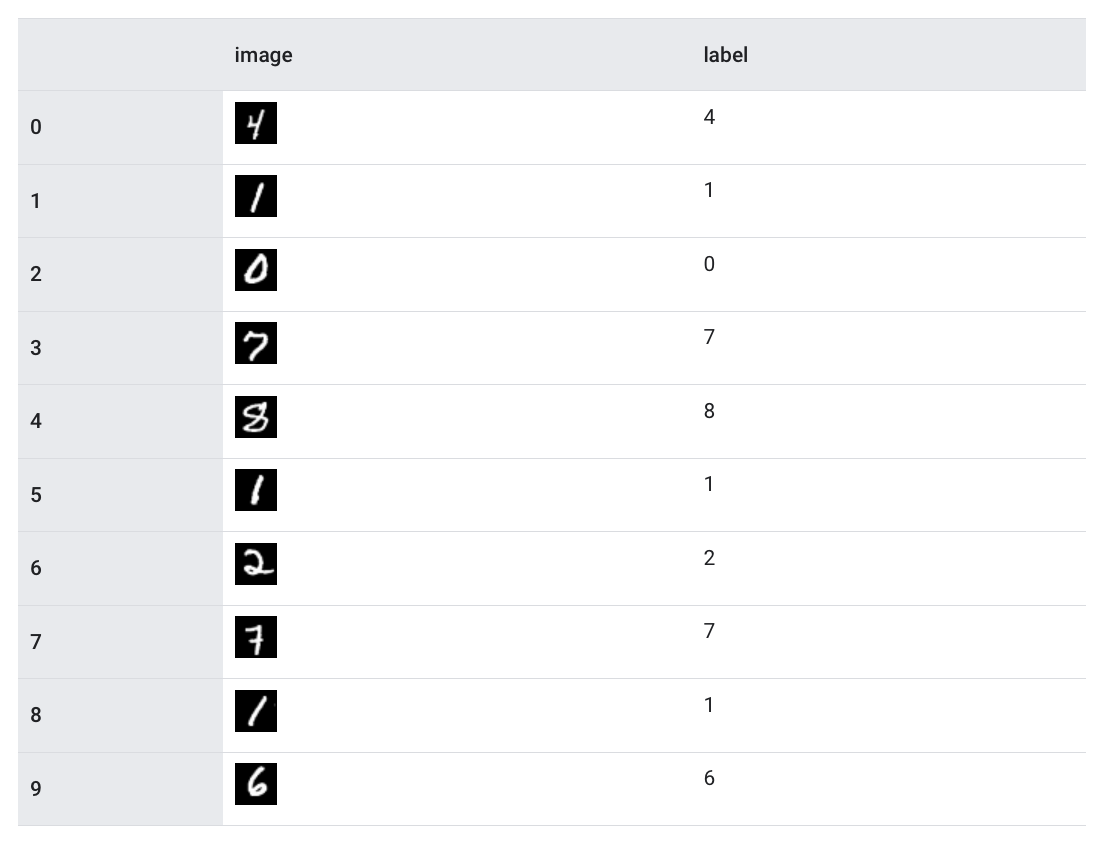
\includegraphics[width=10cm]{mnistExamples.png}
\caption{Examples from the MNIST Data Set}\label{fig:mnistExamples}
\end{figure}

Figure \ref{fig:mnistExamples} shows 10 of the handwritten digits from the MNIST data set, and their respective labels.

I first needed to download the dataset and read it. I decided to retrieve it and some code to read it from Micheal Nielsen's code repository \cite{mnielsenGithub}, to ensure that I get the correct data.

\begin{listing}[H]
(This code has been adapted from Micheal Nielsen's code repository \cite{mnielsenGithub}) \\
\pil{network_training / load_digits_data.py}
\begin{minted}[linenos,breaklines,frame=single,firstnumber=1]{python}
import pickle
import gzip

# loads the MNIST data set
def load_data():
    with gzip.open('data/mnist.pkl.gz', 'rb') as file:
        unpickled = pickle._Unpickler(file)
        unpickled.encoding = 'latin1'
        training_data, validation_data, test_data = unpickled.load()
    return (training_data, validation_data, test_data)
\end{minted}
\caption{Loading in the MNIST data set}\label{cs:loadMNIST}
\end{listing}

The MNIST data set seems to be in the \pil{.pkl.gz} format, which means we must open it with the \pil{gzip} library, and then unpickle it with the \pil{pickle} module.

We can then load the training data, validation data, and testing data from the unpickled and uncompressed file. The 70000 examples are split up into 50000 training examples, 10000 validation examples and 10000 testing examples. I will only be using the 50000 training examples and the 10000 testing examples for the purposes of testing my network.

We now must convert this data into the correct format, to feed into our neural network.

\begin{listing}[H]
\pil{network_training / load_digits_data.py}
\begin{minted}[linenos,breaklines,frame=single,firstnumber=3]{python}
import numpy as np
\end{minted}
(This code has been adapted from Micheal Nielsen's code repository \cite{mnielsenGithub}) \\
\pil{network_training / load_digits_data.py}
\begin{minted}[linenos,breaklines,frame=single,firstnumber=13]{python}
# makes a vector for the output layer from the correct output label
def convert_to_vector(correct_output):
    output_layer = np.zeros((10, 1))
    output_layer[correct_output] = 1
    return output_layer

training_data, _, test_data = load_data()
# convert training data into the right format
training_inputs = [np.reshape(input_data, (784, 1)) for input_data in training_data[0]]
training_outputs = [convert_to_vector(output_data) for output_data in training_data[1]]
training_data = [{
    'input': training_inputs[example],
    'output': training_outputs[example]
} for example in range(len(training_inputs))]
# convert testing data into the right format
test_inputs = [np.reshape(input_data, (784, 1)) for input_data in test_data[0]]
test_outputs = test_data[1]
test_data = [{
    'input': test_inputs[example],
    'output': test_outputs[example]
} for example in range(len(test_inputs))]
\end{minted}
\caption{Converting the MNIST data to the right format}\label{cs:MNISTtoRightFormat}
\end{listing}

First, we must load the data using the function defined in the previous code snippet. It returns all 3 data sets, but I only need the training one and the testing one, so in place of the validation data I have used an underscore, to show that that return variable will not be used.

As each image is made of 784 grayscale pixels, that means our input layer must have 784 neurons, and so should therefore be a matrix with 1 column and 784 rows (hence why we \pil{np.reshape} it).

The neural network will have 10 neurons in the output layer, representing the confidence in each digit. For example, an output layer of \pil{[0, 0, 0.9, 0, 0, 0.1, 0, 0, 0, 0]} would suggest that the network believe that particular digit is a 2, as \pil{0.9} $>$ all of the other activations.

Therefore, we must write a function, \pil{def convert_to_vector}, which takes in the correct output number, and creates the output layer vector from it. This will be a matrix with 10 rows and 1 column, filled with 0s, except for at the index of the correct answer, where it will be 1. This function must then be applied to all items in the training outputs.

We can then save these 2 variables, \pil{training_inputs} and \pil{training_outputs} to a dictionary ready for the neural network to read.

This process must be repeated for the test data, except we don't need to convert the output to a vector, as we will instead be converting the vector generated by the network into a formal prediciton (1 digit).

\begin{listing}[H]
\pil{network_training / load_digits_data.py}
\begin{minted}[linenos,breaklines,frame=single,firstnumber=29]{python}
# save data to a file
with open(f'data/digits.pkl', 'wb') as file:
    pickle.dump({'training': training_data, 'testing': test_data}, file)
\end{minted}
\caption{Saving the MNIST data to a file}\label{cs:MNISTtoFile}
\end{listing}

Once we have all of the training data and testing data, we can save it to a file, again using \pil{pickle}.

\begin{center}
\csvloop{
    file=data/minitests.csv,
    no head,
    column count=6,
    column names={1=\mtestID, 2=\mtestName, 3=\mtestInputs, 4=\mtestType, 5=\mtestExpectedOutputs, 6=\mtestRealOutputs},
    filter ifthen={\equal{\mtestID}{$t_{35}$}\OR\equal{\mtestID}{\textbf{No.}}},
    before reading={
        \begin{longtable}{|m{1cm}|m{3cm}|m{3cm}|m{2cm}|m{3cm}|m{3cm}|}
        \hline
    },
    command=\csvlinetotablerow,
    late after line=\\\hline,
    after reading={
        \caption{Testing Table for Code Snippets \ref{cs:loadMNIST}, \ref{cs:MNISTtoRightFormat} \& \ref{cs:MNISTtoFile}}
        \end{longtable}
    }
}
\end{center}

\begin{listing}[H]
\pil{network_training / train_digits.py}
\begin{minted}[linenos,breaklines,frame=single,firstnumber=1]{python}
import pickle

# load the training data from the file
with open('data/digits.pkl', 'rb') as file:
    data = pickle.load(file)
training_data = data['training']

# import the class MultilayerPerceptron from the neural_network.py file
from neural_network import MultilayerPerceptron
\end{minted}
\caption{Loading the MNIST Training Data}\label{cs:loadTrainingMNIST}
\end{listing}

In a different file, for training the network, we can then read this data and select only the training data from the dictionary.

We then need to import the \pil{class MultilayerPerceptron} from the \pil{neural_network.py} file. Unfortunately, this returned a \pil{ModuleNotFoundError}.

\begin{figure}[H]
\centering
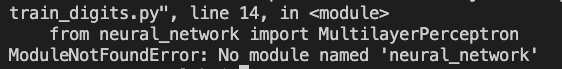
\includegraphics[width=14cm]{ss9.1.png}
\caption{\pil{ModuleNotFoundError}}\label{fig:ss9.1}
\end{figure}

This is because the current file (\pil{train_digits.py}) is in another directory (\pil{network_training}) from \pil{neural_network.py}. We must therefore import from a parent directory.

I did not know how to resolve this issue, but after researching the proble, I found a GeeksforGeeks solution \cite{geeksforGeeksParentDir} on how to import from a parent directory.

\begin{listing}[H]
(This code has been adapted from this GeeksforGeeks solution: \cite{geeksforGeeksParentDir}) \\
\pil{network_training / train_digits.py}
\begin{minted}[linenos,breaklines,frame=single,firstnumber=8]{python}
# import the class MultilayerPerceptron from the neural_network.py file
import os
import sys
current = os.path.dirname(os.path.realpath(__file__))
parent = os.path.dirname(current)
sys.path.append(parent)
from neural_network import MultilayerPerceptron
\end{minted}
\caption{Importing from a Parent Directory}\label{cs:importParent}
\end{listing}

This solution seems to be getting around the problem by finding the ``real path'' of the current file (\pil{__file__}), finding its parent directory, and adding that to the \pil{sys.path}, which means we can now accecss files from the parent directory (namely, \pil{neural_network.py}).

\begin{center}
\csvloop{
    file=data/minitests.csv,
    no head,
    column count=6,
    column names={1=\mtestID, 2=\mtestName, 3=\mtestInputs, 4=\mtestType, 5=\mtestExpectedOutputs, 6=\mtestRealOutputs},
    filter ifthen={\equal{\mtestID}{$t_{36}$}\OR\equal{\mtestID}{\textbf{No.}}},
    before reading={
        \begin{longtable}{|m{1cm}|m{3cm}|m{3cm}|m{2cm}|m{3cm}|m{3cm}|}
        \hline
    },
    command=\csvlinetotablerow,
    late after line=\\\hline,
    after reading={
        \caption{Testing Table for Code Snippets \ref{cs:loadTrainingMNIST} \& \ref{cs:importParent}}
        \end{longtable}
    }
}
\end{center}

\begin{listing}[H]
\pil{network_training / train_digits.py}
\begin{minted}[linenos,breaklines,frame=single,firstnumber=16]{python}
# train the network
network = MultilayerPerceptron([784, 16, 16, 10])
network.train(training_data, 1000, 10, 1)
network.save_model('digits')
\end{minted}
\caption{Training a Neural Network on the MNIST Data Set}\label{cs:trainOnMNIST}
\end{listing}

Now that we have successfully imported the \pil{class MultilayerPerceptron}, we can attempt to train it. We must first instantiate a \pil{MultilayerPerceptron}, with 784 neurons in the input layer and 10 neurons in the output layer. The number of neurons in the hidden layer(s), and the number of hidden layers have no requirements, so I have arbitrarily decided to make 2 hidden layers, each with 16 neurons.

We can then call the \pil{train} method, passing in the training data. Again, I have arbitrarily decided that the mini batch size is 1000, the number of epochs is 10, and the learning rate is 1.

Once it is fully trained, we can save the weights and biases to a file, by calling the \pil{save_model} method.

\begin{listing}[H]
\pil{neural_network.py / class MultilayerPerceptron / def train}
\begin{minted}[linenos,breaklines,frame=single,firstnumber=90]{python}
            for num, mini_batch in enumerate(mini_batches):
                print(f' mini batch {num}/{len(mini_batches)}...') # log message
\end{minted}
\caption{Adding another log message}\label{cs:moreLogs}
\end{listing}

Each epoch was taking a very long time, so I decided to add another log message, for each mini batch.

\begin{center}
\csvloop{
    file=data/minitests.csv,
    no head,
    column count=6,
    column names={1=\mtestID, 2=\mtestName, 3=\mtestInputs, 4=\mtestType, 5=\mtestExpectedOutputs, 6=\mtestRealOutputs},
    filter ifthen={\equal{\mtestID}{$t_{37}$}\OR\equal{\mtestID}{\textbf{No.}}},
    before reading={
        \begin{longtable}{|m{1cm}|m{3cm}|m{3cm}|m{2cm}|m{3cm}|m{3cm}|}
        \hline
    },
    command=\csvlinetotablerow,
    late after line=\\\hline,
    after reading={
        \caption{Testing Table for Code Snippets \ref{cs:trainOnMNIST} \& \ref{cs:moreLogs}}
        \end{longtable}
    }
}
\end{center}

\begin{listing}[H]
\pil{network_training / test_digits.py}
\begin{minted}[linenos,breaklines,frame=single,firstnumber=1]{python}
import pickle

# load the test data from the file
with open('data/digits.pkl', 'rb') as file:
    data = pickle.load(file)
testing_data = data['testing']

# import the class MultilayerPerceptron from the neural_network.py file
import os
import sys
current = os.path.dirname(os.path.realpath(__file__))
parent = os.path.dirname(current)
sys.path.append(parent)
from neural_network import MultilayerPerceptron
\end{minted}
\caption{Loading the MNIST Testing Data}\label{cs:loadTestMNIST}
\end{listing}

In order to test our trained neural network, we must first do the same thing as in the training file, which is loading the testing data from the file, and then importing the \pil{class MultilayerPerceptron} from the parent directory.

\begin{center}
\csvloop{
    file=data/minitests.csv,
    no head,
    column count=6,
    column names={1=\mtestID, 2=\mtestName, 3=\mtestInputs, 4=\mtestType, 5=\mtestExpectedOutputs, 6=\mtestRealOutputs},
    filter ifthen={\equal{\mtestID}{$t_{38}$}\OR\equal{\mtestID}{\textbf{No.}}},
    before reading={
        \begin{longtable}{|m{1cm}|m{3cm}|m{3cm}|m{2cm}|m{3cm}|m{3cm}|}
        \hline
    },
    command=\csvlinetotablerow,
    late after line=\\\hline,
    after reading={
        \caption{Testing Table for Code Snippet \ref{cs:loadTestMNIST}}
        \end{longtable}
    }
}
\end{center}

\begin{listing}[H]
\pil{network_training / test_digits.py}
\begin{minted}[linenos,breaklines,frame=single,firstnumber=16]{python}
# iterate over each of the testing examples and see how many it gets right
network = MultilayerPerceptron([784, 16, 16, 10])
network.load_model('models/digits.pkl')
success = 0
for total_so_far, example in enumerate(testing_data):
    prediction = network.predict(example['input'])
    list_of_probabilities = [prediction.item(x,0) for x in range(10)]
    if list_of_probabilities.index(max(list_of_probabilities)) == example['output']:
        success += 1
    print(f'after {total_so_far+1} examples, the success rate is {(success/(total_so_far+1))*100}%')
\end{minted}
\caption{Testing the Neural Network on the MNIST Data Set}\label{cs:testOnMNIST}
\end{listing}

To test it, again we must first instantiate a \pil{MultilayerPerceptron}, with the same layer sizes, and then use the \pil{load} method to set the weights and biases to that of the trained network.

Then, we must iterate over each of the pieces of testing data, and make a prediction. Currently, this prediction is a column vector with 10 entries, one of which should hopefully be much larger than the rest, which is the network's prediction. To get this prediction, we must find the index of the maximum value of the column vector. If it is the same as the example's output (what the number is supposed to be), then the network has successfully predicted the digit.

After each prediction, we can print the current success rate, to see how it evolves over time.

\begin{center}
\csvloop{
    file=data/minitests.csv,
    no head,
    column count=6,
    column names={1=\mtestID, 2=\mtestName, 3=\mtestInputs, 4=\mtestType, 5=\mtestExpectedOutputs, 6=\mtestRealOutputs},
    filter ifthen={\equal{\mtestID}{$t_{39}$}\OR\equal{\mtestID}{\textbf{No.}}},
    before reading={
        \begin{longtable}{|m{1cm}|m{3cm}|m{3cm}|m{2cm}|m{3cm}|m{3cm}|}
        \hline
    },
    command=\csvlinetotablerow,
    late after line=\\\hline,
    after reading={
        \caption{Testing Table for Code Snippet \ref{cs:testOnMNIST}}
        \end{longtable}
    }
}
\end{center}

\begin{figure}[H]
\centering
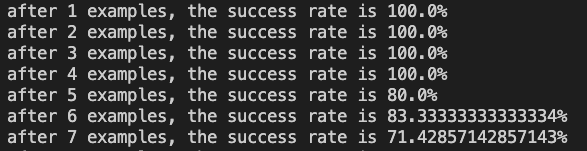
\includegraphics[width=14cm]{ss9.2.png}
\caption{Output for the first 7 training examples}\label{fig:ss9.2}
\end{figure}

Figure \ref{fig:ss9.2} shows the output for the first 7 examples. This shows that it got the first 4 correct, then 1 wrong, then another one correct, and then another one wrong.

\begin{figure}[H]
\centering
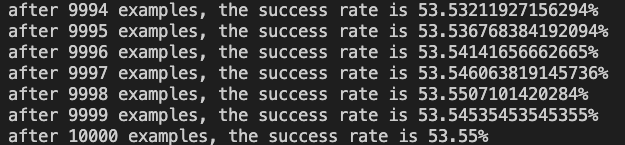
\includegraphics[width=14cm]{ss9.3.png}
\caption{Output for the last 7 training examples}\label{fig:ss9.3}
\end{figure}

Figure \ref{fig:ss9.3} shows the output for the last 7 examples. This shows that it has converged on a success rate of around $53.55\%$. This is a good result, but not great as it still got about half of them wrong.

\begin{listing}[H]
\pil{network_training / train_digits.py}
\begin{minted}[linenos,breaklines,frame=single,firstnumber=18]{python}
network.train(training_data, 10, 30, 3)
\end{minted}
\caption{Improving the Training Paremeters}\label{cs:improveTrainingParameters}
\end{listing}

If we adjust the training parameters, to have smaller mini batches, more epochs and a greater leanring rate, the success rate will increase. (To get a new model, we must of course re-run \pil{train_digits.py} and \pil{test_digits.py})

\begin{figure}[H]
\centering
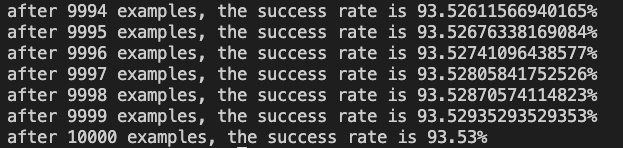
\includegraphics[width=14cm]{ss9.4.png}
\caption{Improved Output for the last 7 training examples}\label{fig:ss9.4}
\end{figure}

Figure \ref{fig:ss9.4} shows the output for the last 7 examples, with new training parameters. We now converge on around $93.53\%$, which is much better.

If the training didn't work, then the success rate should be around $10\%$, as it would just be picking digits at random, and so it would have a $\frac{1}{10}$ chance of getting it right. $93.53\%$ is much greater than $10\%$, and so I believe there is sufficient evidence to suggest that the neural network, and the backpropogation algorithm is in fact working.

\begin{center}
\csvloop{
    file=data/minitests.csv,
    no head,
    column count=6,
    column names={1=\mtestID, 2=\mtestName, 3=\mtestInputs, 4=\mtestType, 5=\mtestExpectedOutputs, 6=\mtestRealOutputs},
    filter ifthen={\equal{\mtestID}{$T_{5}$}\OR\equal{\mtestID}{\textbf{No.}}},
    before reading={
        \begin{longtable}{|m{1cm}|m{3cm}|m{3cm}|m{2cm}|m{3cm}|m{3cm}|}
        \hline
    },
    command=\csvlinetotablerow,
    late after line=\\\hline,
    after reading={
        \caption{$T_{5}$ Testing Table (for Code Snippet \ref{cs:improveTrainingParameters})}\label{table:t5testing}
        \end{longtable}
    }
}
\end{center}

\stepcounter{parts}
\subsection{Part \theparts{} -- Training the Neural Network}\label{sec:trainNetwork}

Now it is time to trian the neural network to predict the HDI of a given area.

\begin{listing}[H]
\pil{network_training / load_hdi_data.py}
\begin{minted}[linenos,breaklines,frame=single,firstnumber=1]{python}
import csv
import numpy as np

# read csv file
with open('data/training_data.csv', 'r') as file:
    reader = csv.DictReader(file)
    hdiData = []
    for record in reader:
        # convert it to the right format
        hdiData.append({
            "input": np.matrix([[1000 if factor == '' else float(factor)] for factor in list(record.values())[4:]]),
            "output": np.matrix([[float(record['hdi'])]])
        })
\end{minted}
\caption{Loading the HDI Data}\label{cs:loadHDIdata}
\end{listing}

First, we must convert the HDI data into the right format. We can read the \pil{.csv} file using the same methods as before, except when we go to append each record, we must slightly change the format.

Currently, each record is a dictionary of all the factors, along with some extra information (such as the name of the region). The input data should be a list of factors (as a column vector), which currently start at index \pil{4}. Each of these factors is currently of type \pil{str}, so we must convert it to a \pil{float}. Some of the factors are also currently an empty string, which correspond to average distance factors in regions that have 0 of that building. I have set these to 1000, as that is larger than every other average distance factor.

The output should just be the HDI, which is located at key \pil{'hdi'}.

\begin{listing}[H]
\pil{network_training / load_hdi_data.py}
\begin{minted}[linenos,breaklines,frame=single,firstnumber=3]{python}
import random
import pickle
\end{minted}
\pil{network_training / load_hdi_data.py}
\begin{minted}[linenos,breaklines,frame=single,firstnumber=17]{python}
# split the data set into training and testing
def test_train_split(data_set, proportion_train):
    random.shuffle(data_set)
    return {
        "training": data_set[:int((len(data_set)*proportion_train)//1)],
        "testing": data_set[int((len(data_set)*proportion_train)//1):]
    }

hdiData = test_train_split(hdiData, 0.9)
# save data to a file
with open(f'data/hdi.pkl', 'wb') as file:
    pickle.dump(hdiData, file)
\end{minted}
\caption{Splitting into Testing and Training Data}\label{cs:testTrainSplit}
\end{listing}

We then must randomly split the data set into training and testing data. For this, I have written a function, \pil{def test_train_split}, which will take in a data set and a proportion which should be training data.

If we multiply the length of the data set by the proportion, we get the index of the final piece of data which should be for training. Therefore, everything before that should be training and everything after it should be testing.

After we have split the data set, we can again save it to file as we have done before.

\begin{center}
\csvloop{
    file=data/minitests.csv,
    no head,
    column count=6,
    column names={1=\mtestID, 2=\mtestName, 3=\mtestInputs, 4=\mtestType, 5=\mtestExpectedOutputs, 6=\mtestRealOutputs},
    filter ifthen={\equal{\mtestID}{$t_{40}$}\OR\equal{\mtestID}{$t_{41}$}\OR\equal{\mtestID}{\textbf{No.}}},
    before reading={
        \begin{longtable}{|m{1cm}|m{3cm}|m{3cm}|m{2cm}|m{3cm}|m{3cm}|}
        \hline
    },
    command=\csvlinetotablerow,
    late after line=\\\hline,
    after reading={
        \caption{Testing Table for Code Snippets \ref{cs:loadHDIdata} \& \ref{cs:testTrainSplit}}
        \end{longtable}
    }
}
\end{center}

\begin{listing}[H]
\pil{network_training / train_hdi.py}
\begin{minted}[linenos,breaklines,frame=single,firstnumber=1]{python}
import pickle

# load the training data from the file
with open('data/hdi.pkl', 'rb') as file:
    data = pickle.load(file)
training_data = data['training']

# import the class MultilayerPerceptron from the neural_network.py file
import os
import sys
current = os.path.dirname(os.path.realpath(__file__))
parent = os.path.dirname(current)
sys.path.append(parent)
from neural_network import MultilayerPerceptron

# train the network
network = MultilayerPerceptron([24, 10, 10, 1])
network.train(training_data, 10, 30, 3)
network.save_model('hdi-temp')
\end{minted}
\caption{Training the Neural Network on HDI}\label{cs:trainHDI}
\end{listing}

We can then train the neural network on the HDI training data in exactly the same way as we did for the MNIST handwritten digits.

Except, this time we must have 24 neurons in the input layer (for each of the 24 factors), and 1 neuron in the output layer. I initially decided to have 2 hidden layers, each with 10 neurons, and to keep the remaining training parameters the same. (mini batch size $=10$, number of epochs $=30$, learning rate $=3$)

\begin{center}
\csvloop{
    file=data/minitests.csv,
    no head,
    column count=6,
    column names={1=\mtestID, 2=\mtestName, 3=\mtestInputs, 4=\mtestType, 5=\mtestExpectedOutputs, 6=\mtestRealOutputs},
    filter ifthen={\equal{\mtestID}{$t_{42}$}\OR\equal{\mtestID}{\textbf{No.}}},
    before reading={
        \begin{table}[H]
        \centering
        \begin{tabular}{|m{1cm}|m{3cm}|m{3cm}|m{2cm}|m{3cm}|m{3cm}|}
        \hline
    },
    command=\csvlinetotablerow,
    late after line=\\\hline,
    after reading={
        \end{tabular}
        \caption{Testing Table for Code Snippet \ref{cs:trainHDI}}
        \end{table}
    }
}
\end{center}

\begin{listing}[H]
\pil{network_training / test_hdi.py}
\begin{minted}[linenos,breaklines,frame=single,firstnumber=1]{python}
import pickle

# load the test data from the file
with open('data/hdi.pkl', 'rb') as file:
    data = pickle.load(file)
testing_data = data['testing']

# import the class MultilayerPerceptron from the neural_network.py file
import os
import sys
current = os.path.dirname(os.path.realpath(__file__))
parent = os.path.dirname(current)
sys.path.append(parent)
from neural_network import MultilayerPerceptron

# iterate over each of the testing examples and see how many it gets right
network = MultilayerPerceptron([24, 10, 10, 1])
network.load_model('models/hdi-temp.pkl')
\end{minted}
\caption{Preparing to Test on the HDI}\label{cs:preTestHDI}
\end{listing}

When we test the network, we should again load it in exactly the same way as with the MNIST Data Set, with the same changes to the hidden layers.

\begin{listing}[H]
\pil{network_training / test_hdi.py}
\begin{minted}[linenos,breaklines,frame=single,firstnumber=19]{python}
differences = []
for num, example in enumerate(testing_data):
    correctAnswer = example["output"].item(0,0)
    prediction = round(network.predict(example['input']).item(0,0), 3)
    difference = round(abs(correctAnswer-prediction), 3)
    print(f'({num}) correct output: {correctAnswer}, prediction: {prediction}, difference: {difference}')
    differences.append(difference)

import numpy as np
print(f'average difference: {np.mean(differences)}')
\end{minted}
\caption{Testing the Neural Network on HDI}\label{cs:testHDI}
\end{listing}

As the output for this network is slightly different, we should test it in a different way. The correct HDI is given by the \pil{'output'} of the testing example, and we can compare that with the prediction.

At each stage, we round our values to 3 decimal places, as this is what HDI is most commonly quoted to. At the end, we can take the mean to find an average differene.

\begin{center}
\csvloop{
    file=data/minitests.csv,
    no head,
    column count=6,
    column names={1=\mtestID, 2=\mtestName, 3=\mtestInputs, 4=\mtestType, 5=\mtestExpectedOutputs, 6=\mtestRealOutputs},
    filter ifthen={\equal{\mtestID}{$t_{43}$}\OR\equal{\mtestID}{\textbf{No.}}},
    before reading={
        \begin{longtable}{|m{1cm}|m{3cm}|m{3cm}|m{2cm}|m{3cm}|m{3cm}|}
        \hline
    },
    command=\csvlinetotablerow,
    late after line=\\\hline,
    after reading={
        \caption{Testing Table for Code Snippets \ref{cs:preTestHDI} \& \ref{cs:testHDI}}
        \end{longtable}
    }
}
\end{center}

\begin{figure}[H]
\centering
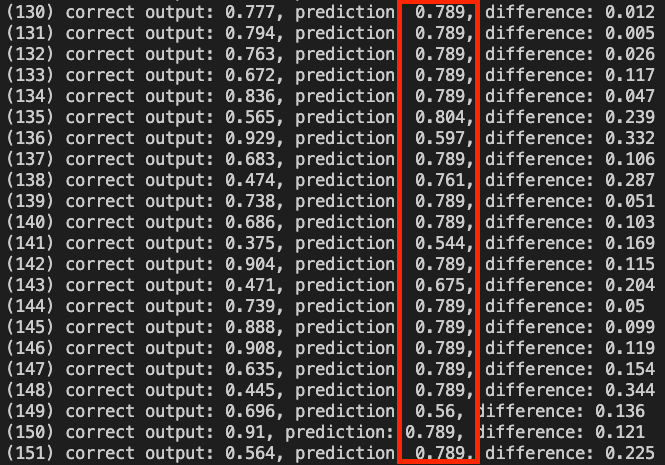
\includegraphics[width=13cm]{ss10.1.png}
\caption{Some HDI Predictions}\label{fig:ss10.1}
\end{figure}

Figure \ref{fig:ss10.1} shows some of the network's predictons. As you can see, most of them are the same, with a prediction of 0.789, which is obviously not ideal.

The first thing I thought of to ammend this is to change the scale of the factors.

\begin{listing}[H]
\pil{network_training / load_hdi_data.py}
\begin{minted}[linenos,breaklines,frame=single,firstnumber=11]{python}
        # convert it to the right format
        hdiData.append({
            "input": np.matrix([[100 if factor == '' else float(factor)/10 if index <= 11 else float(factor)] for index, factor in enumerate(list(record.values())[4:])]),
            "output": np.matrix([[float(record['hdi'])]])
        })
\end{minted}
\caption{Dividing some factors by 10}\label{cs:divFactorsBy10}
\end{listing}

Each of the average distance factors often take values in between 1 and 10, but this particular type of neural network often works best with numbers between 0 and 1. Therefore, I have divided each of the average distance factors (at indexes \pil{0} to \pil{11}) by 10, to get most of them in this range.

\begin{center}
\csvloop{
    file=data/minitests.csv,
    no head,
    column count=6,
    column names={1=\mtestID, 2=\mtestName, 3=\mtestInputs, 4=\mtestType, 5=\mtestExpectedOutputs, 6=\mtestRealOutputs},
    filter ifthen={\equal{\mtestID}{$t_{44}$}\OR\equal{\mtestID}{\textbf{No.}}},
    before reading={
        \begin{table}[H]
        \centering
        \begin{tabular}{|m{1cm}|m{3cm}|m{3cm}|m{2cm}|m{3cm}|m{3cm}|}
        \hline
    },
    command=\csvlinetotablerow,
    late after line=\\\hline,
    after reading={
        \end{tabular}
        \caption{Testing Table for Code Snippet \ref{cs:divFactorsBy10}}
        \end{table}
    }
}
\end{center}

The network was still not predicting very well, so I had to adjust the training parameters.

\begin{listing}[H]
\pil{network_training / train_hdi.py}
\begin{minted}[linenos,breaklines,frame=single,firstnumber=16]{python}
# train the network
network = MultilayerPerceptron([24, 18, 12, 6, 3, 1])
network.train(training_data, 5, 50, 0.2)
network.save_model('hdi-temp')
\end{minted}
\pil{network_training / test_hdi.py}
\begin{minted}[linenos,breaklines,frame=single,firstnumber=16]{python}
# iterate over each of the testing examples and see how many it gets right
network = MultilayerPerceptron([24, 18, 12, 6, 3, 1])
network.load_model('models/hdi-temp.pkl')
\end{minted}
\caption{Adjusting the Training Parameters}\label{cs:adjustParameters}
\end{listing}

After many attempts, I ended up with a neural network with 4 hidden layers, each with 18, 12, 6 and 3 neurons respectively, which was trained with a mini batch size of 5, over 50 epochs and a learning rate of 0.2.

\begin{center}
\csvloop{
    file=data/minitests.csv,
    no head,
    column count=6,
    column names={1=\mtestID, 2=\mtestName, 3=\mtestInputs, 4=\mtestType, 5=\mtestExpectedOutputs, 6=\mtestRealOutputs},
    filter ifthen={\equal{\mtestID}{$t_{42}$}\OR\equal{\mtestID}{\textbf{No.}}},
    before reading={
        \begin{longtable}{|m{1cm}|m{3cm}|m{3cm}|m{2cm}|m{3cm}|m{3cm}|}
        \hline
    },
    command=\csvlinetotablerow,
    late after line=\\\hline,
    after reading={
        \caption{Testing Table for Code Snippet \ref{cs:adjustParameters}}
        \end{longtable}
    }
}
\end{center}

\begin{figure}[H]
\centering
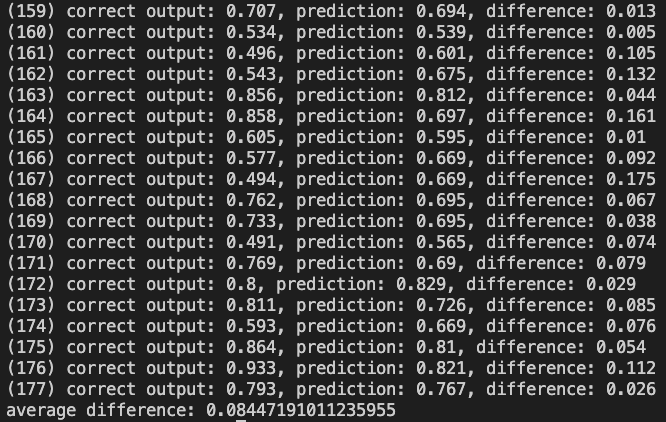
\includegraphics[width=13cm]{ss10.2.png}
\caption{Improved HDI Predictions}\label{fig:ss10.2}
\end{figure}

The variance in these predictions was very high, and the average difference is very low, which is what we need.

\subsection{Review}

\begin{center}
\csvloop{
    file=data/testdata.csv,
    no head,
    column count=5,
    column names={1=\testID, 2=\testName, 3=\testInputs, 4=\testOutputs, 5=\testSuccess},
    filter ifthen={\equal{\testID}{$T_{5}$}\OR\equal{\testID}{\textbf{No.}}},
    before reading={
        \begin{longtable}{|m{1cm}|m{3cm}|m{8cm}|H|m{2cm}|}
        \hline
    },
    command=\csvlinetotablerow,
    late after line=\\\hline,
    after reading={
        \caption{Passed Testing Data for Milestone 2}
        \end{longtable}
    }
}
\end{center}

The fact that we successfully predicted $93.53\%$ of MNIST handwritten digits suggests that $T_{5}$ has been passed, which implies the Success Criteria $S_{5}$ and $S_{6}$ have been met

\begin{center}
\csvloop{
    file=data/successcriteria.csv,
    no head,
    column count=5,
    column names={1=\scID, 2=\scCriterion, 3=\scJustification, 4=\scSuccess, 5=\scEvaluation},
    filter ifthen={\equal{\scID}{$S_{5}$}\OR\equal{\scID}{$S_{6}$}\OR\equal{\scID}{$S_{7}$}\OR\equal{\scID}{\textbf{No.}}},
    before reading={
        \begin{longtable}{|m{1cm}|m{5cm}|m{6cm}|m{2cm}|H}
        \hline
    },
    command=\csvlinetotablerow,
    late after line=\\\hline,
    after reading={
        \caption{Achieved Success Criteria for Milestone 2}
        \end{longtable}
    }
}
\end{center}

I believe $S_{7}$ has also been met, as we have been able to train a neural network which can (vaguely) predict the HDI of a given area.

\section{Milestone 3 -- Initial User Interface}
\subsection{Success Criteria}
By the end of this milestone, I hope to have a fully functioning user interface, in which the user can select their region on a map, predict the HDI of it, and have suggestions made to improve it.
\begin{center}
\csvloop{
    file=data/successcriteria.csv,
    no head,
    column count=5,
    column names={1=\scID, 2=\scCriterion, 3=\scJustification, 4=\scSuccess, 5=\scEvaluation},
    filter ifthen={\equal{\scID}{$S_{8}$}\OR\equal{\scID}{$S_{9}$}\OR\equal{\scID}{$S_{10}$}\OR\equal{\scID}{$S_{11}$}\OR\equal{\scID}{\textbf{No.}}},
    before reading={
        \begin{longtable}{|m{1cm}|m{5cm}|m{8cm}|H H}
        \hline
    },
    command=\csvlinetotablerow,
    late after line=\\\hline,
    after reading={
        \caption{Success Criteria for Milestone 3}
        \end{longtable}
    }
}
\end{center}

To determine if I have met this success criteria, I will be using the following tests:

\begin{center}
\csvloop{
    file=data/testdata.csv,
    no head,
    column count=5,
    column names={1=\testID, 2=\testName, 3=\testInputs, 4=\testOutputs, 5=\testSuccess},
    filter ifthen={\equal{\testID}{$T_{6}$}\OR\equal{\testID}{$T_{7}$}\OR\equal{\testID}{$T_{8}$}\OR\equal{\testID}{\textbf{No.}}},
    before reading={
        \begin{longtable}{|m{1cm}|m{3cm}|m{5cm}|m{5cm}|H}
        \hline
    },
    command=\csvlinetotablerow,
    late after line=\\\hline,
    after reading={
        \caption{Testing Data for Milestone 3}
        \end{longtable}
    }
}
\end{center}

\stepcounter{parts}
\subsection{Part \theparts{} -- Drawing on the Map}

I believe that having a map to draw on is the most important thing in the GUI, so I will be implemented that first.

\begin{listing}[H]
\pil{app.py}
\begin{minted}[linenos,breaklines,frame=single,firstnumber=1]{python}
import gradio as gr

# structure of the UI
with gr.Blocks() as app:
    pass

# launch the UI
app.launch()
\end{minted}
\caption{Initial Gradio Framework}\label{cs:gradioFramework}
\end{listing}

Here, I am using the \pil{gradio} library to begin to define the interface. Gradio uses context managers (\pil{with} statement) to make the structure of the GUI very readable and easy to understand (this will become more apparent when we add more and more elements).

Gradio offers many types of interface, but the one I will be using is the \pil{Blocks} interface, which allows for the most customisation. For now, we have no structure to add, so we can just \pil{pass}.

Once we have defined the GUI, we can call the \pil{launch} method on the app.

\begin{figure}[H]
\centering
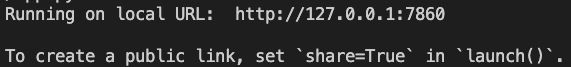
\includegraphics[width=14cm]{ss11.1.png}
\caption{Launching the Gradio App}\label{fig:ss11.1}
\end{figure}

Running this code produces the output shown in Figure \ref{fig:ss11.1}. When we called the \pil{launch} method, it initialised the gradio interface on port \pil{7860}, of the localhost IP address (\pil{127.0.0.1}). It also tells us that we could create a public link, which I will be doing later to share with my stakeholders.

\begin{figure}[H]
\centering
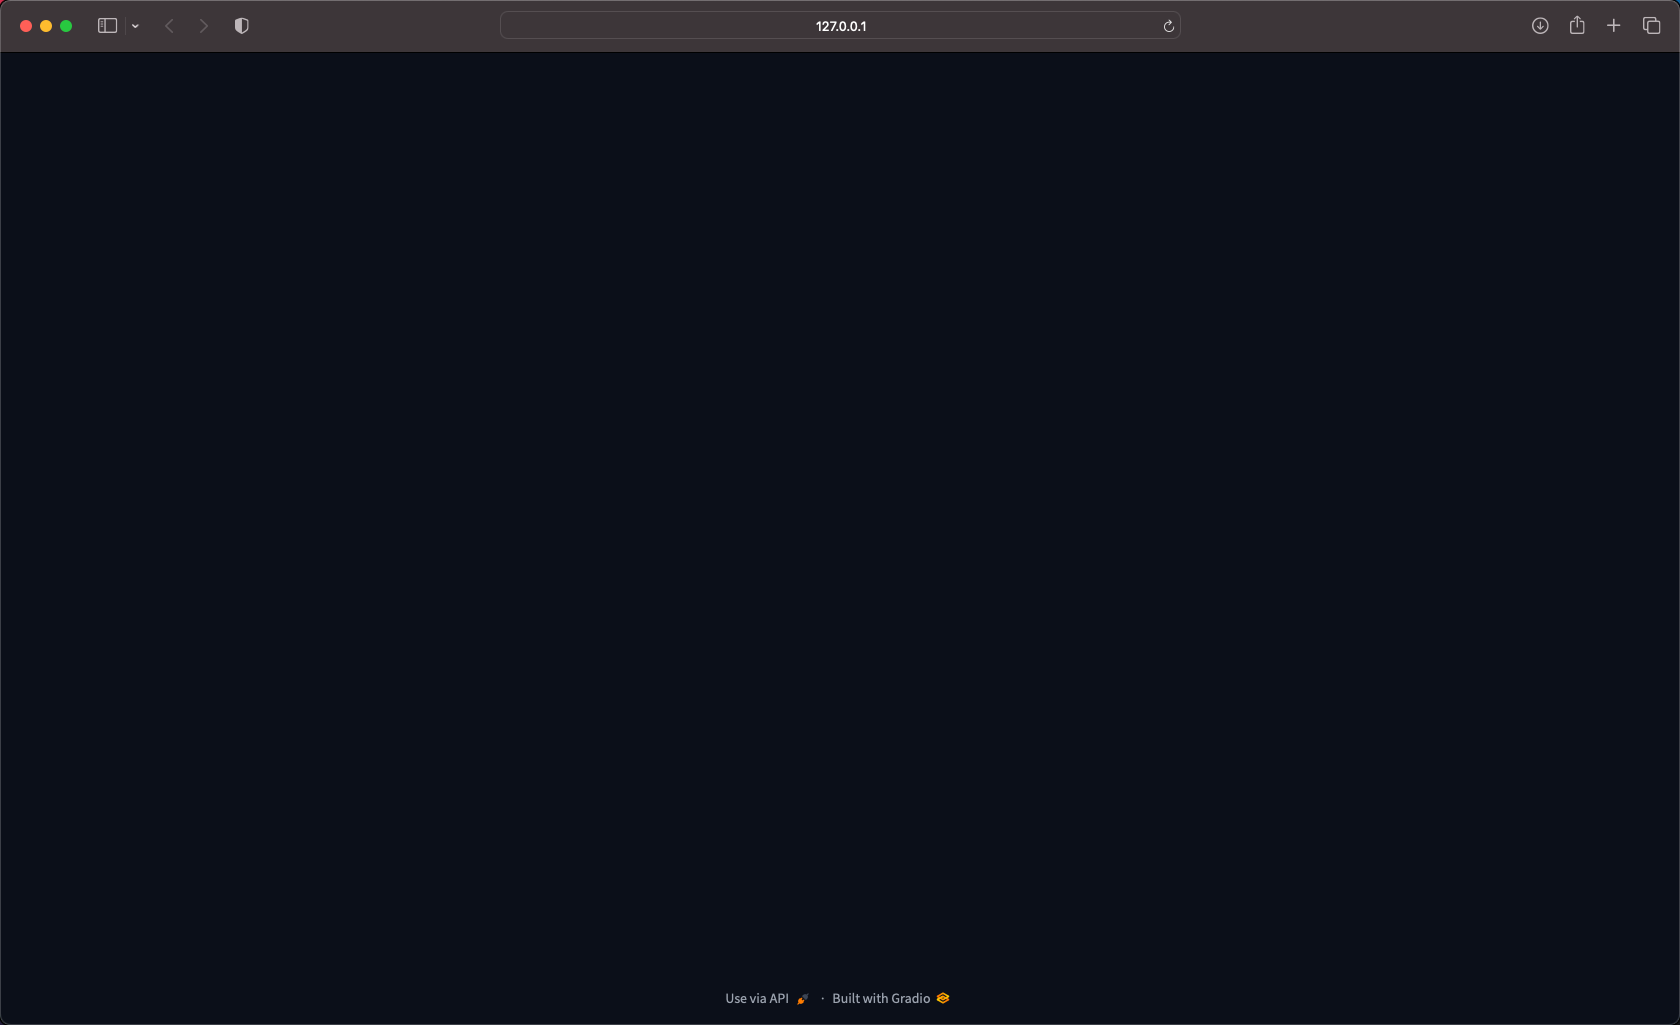
\includegraphics[width=14cm]{ss11.2.png}
\caption{Empty Gradio UI}\label{fig:ss11.2}
\end{figure}

Following the link \pil{http://127.0.0.1:7860} takes us to this empty gradio interface. Once we add components, they will show up here.

\begin{center}
\csvloop{
    file=data/minitests.csv,
    no head,
    column count=6,
    column names={1=\mtestID, 2=\mtestName, 3=\mtestInputs, 4=\mtestType, 5=\mtestExpectedOutputs, 6=\mtestRealOutputs},
    filter ifthen={\equal{\mtestID}{$t_{45}$}\OR\equal{\mtestID}{\textbf{No.}}},
    before reading={
        \begin{longtable}{|m{1cm}|m{3cm}|m{3cm}|m{2cm}|m{3cm}|m{3cm}|}
        \hline
    },
    command=\csvlinetotablerow,
    late after line=\\\hline,
    after reading={
        \caption{Testing Table for Code Snippet \ref{cs:gradioFramework}}
        \end{longtable}
    }
}
\end{center}

\begin{listing}[H]
\pil{app.py}
\begin{minted}[linenos,breaklines,frame=single,firstnumber=2]{python}
import folium
from folium.plugins import Draw

# initialise the map for drawing on
foliumMap = folium.Map()
draw = Draw(
    export=False,
    position='topleft',
    draw_options={
        'polyline': False,
        'circlemarker': False,
        'polygon': {'allowIntersection': False},
        'marker': False,
        'circle': False,
        'rectangle': False,
    },
    edit_options={'poly': {'allowIntersection': False}}
)
draw.add_to(foliumMap)
\end{minted}
\caption{Initialising the Map}\label{cs:initialiseDrawingMap}
\end{listing}

Next, we must also import the \pil{folium} library, which lets us create interactive maps.

First, we can make an instance of the \pil{class Map}, and save that to a variable. To be able to draw on it, we must also make an instance of the \pil{class Draw}, and then add that to the map at the end.

The \pil{class Draw} has many attributes which must be set. Namely, specifying \pil{position} to be \pil{'topleft'} will make the drawing tools appear on the top left. Setting most of the \pil{draw_options} to \pil{False} except for \pil{'polygon'} (which in turn has \pil{'allowIntersection'} set to \pil{False}) ensures that the user can only draw polygons, and the polygons should not be able to self intersect.

\begin{listing}[H]
\pil{app.py}
\begin{minted}[linenos,breaklines,frame=single,firstnumber=2]{python}
from gradio_folium import Folium
\end{minted}
\pil{app.py}
\begin{minted}[linenos,breaklines,frame=single,firstnumber=23]{python}
# structure of the UI
with gr.Blocks() as app:
    map = Folium(value=foliumMap)
\end{minted}
\caption{Adding the Map to the GUI}\label{cs:addMapToGUI}
\end{listing}

To add this to the gradio interface, we must first import the \pil{Folium} element from the \pil{gradio_folium} library, and then add this to our \pil{Blocks} interface. If we save this to a variable, \pil{map}, we will be able to access and update it. We also have zoom in and out buttons in the top left as well.

\begin{figure}[H]
\centering
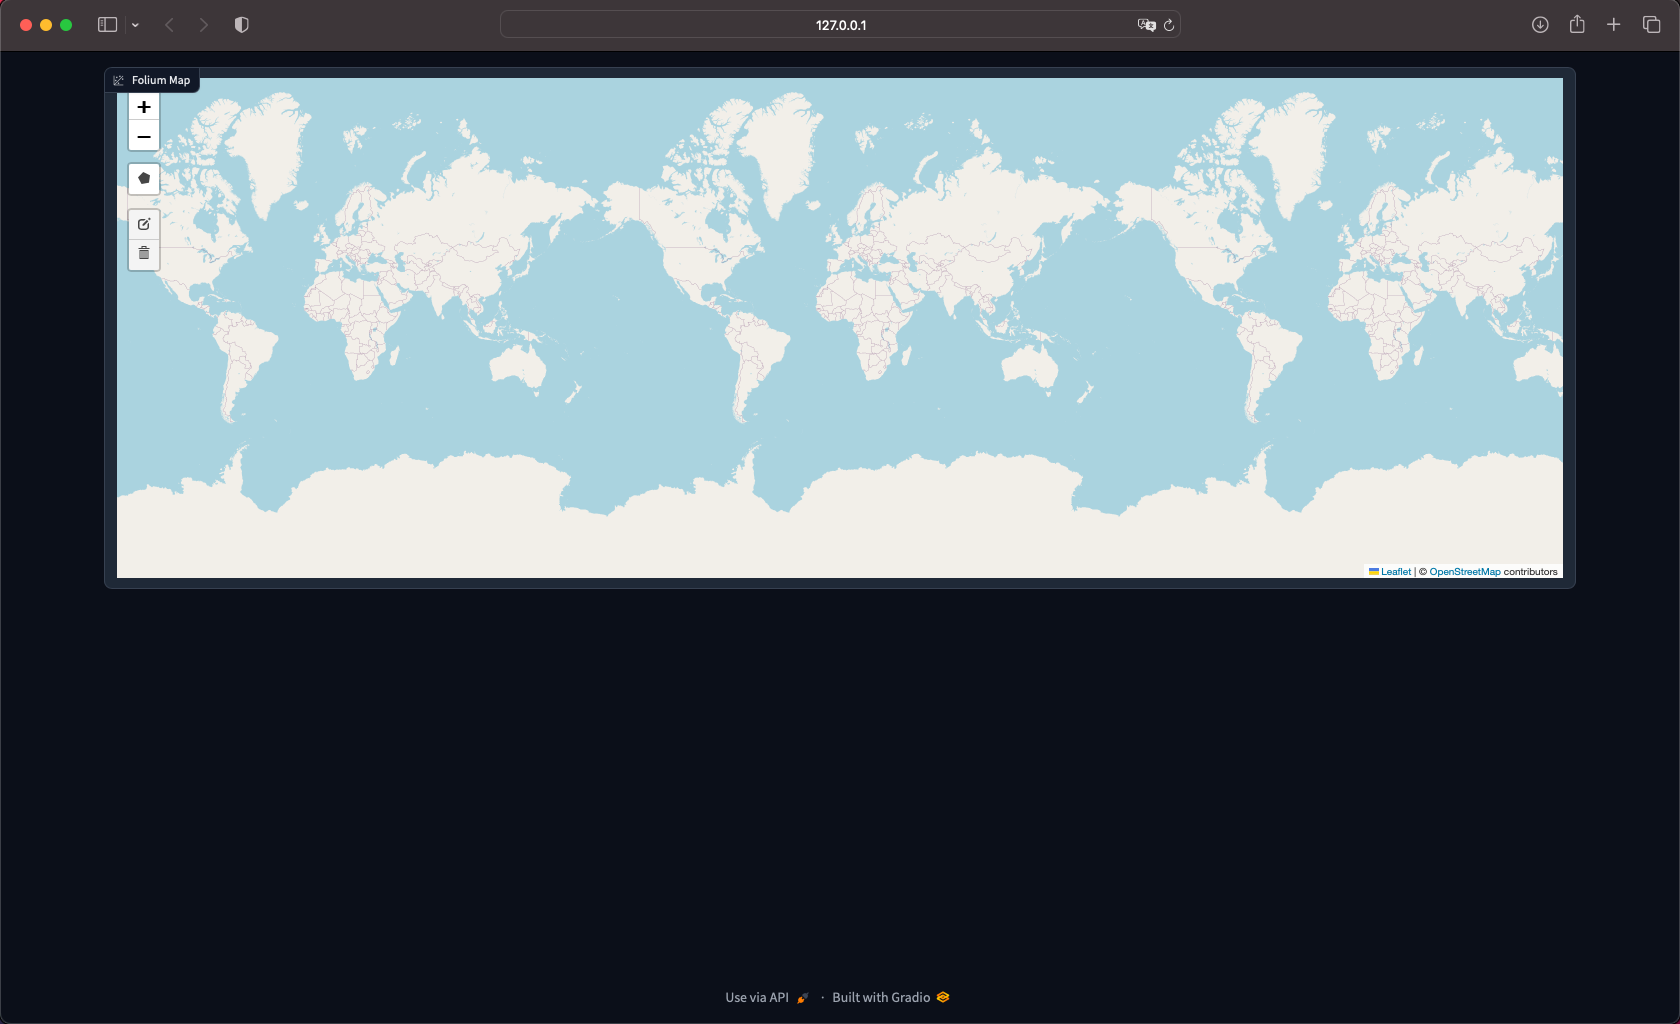
\includegraphics[width=14cm]{ss11.3.png}
\caption{Map Added to GUI}\label{fig:ss11.3}
\end{figure}

Figure \ref{fig:ss11.3} shows the current output for the program, with the drawing tools shown in the top left of the map.

Users can also use the scroll wheel to zoom in and out of the map if they wish. By default, the mouse will drag around the map, but if the user clicks the pentagon icon, using the mouse will then begin to draw a polygon.

\begin{figure}[H]
\centering
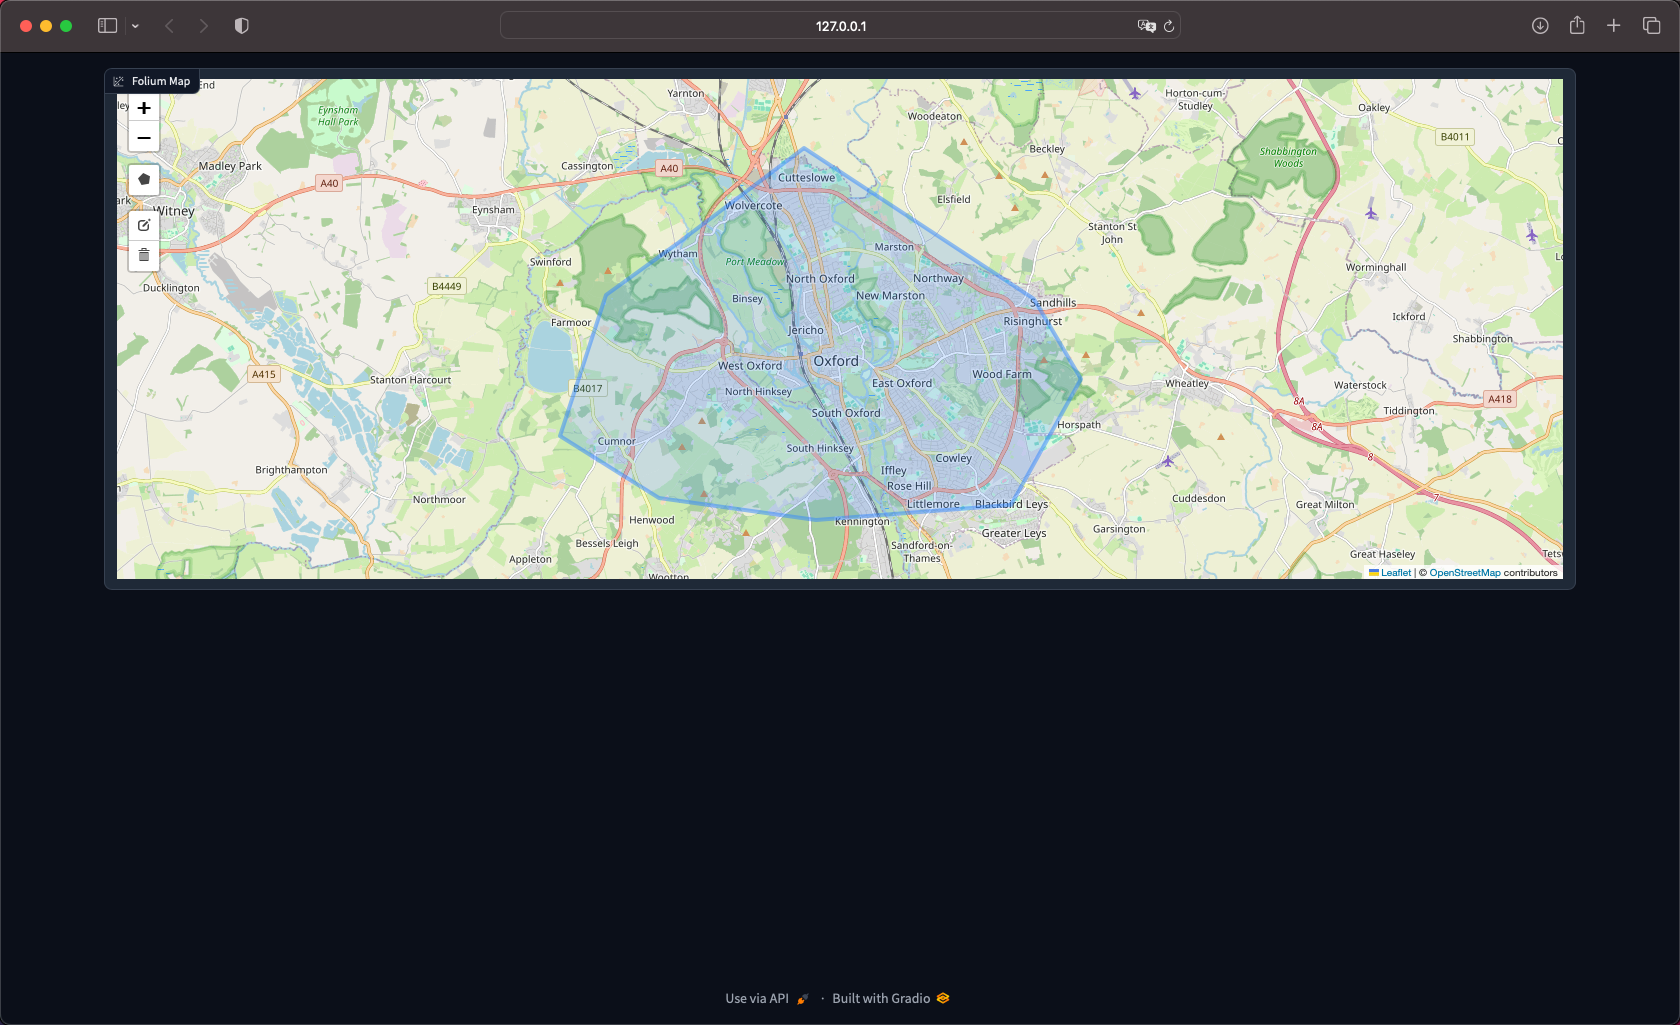
\includegraphics[width=14cm]{ss11.4.png}
\caption{Drawing a Region}\label{fig:ss11.4}
\end{figure}

\begin{center}
\csvloop{
    file=data/minitests.csv,
    no head,
    column count=6,
    column names={1=\mtestID, 2=\mtestName, 3=\mtestInputs, 4=\mtestType, 5=\mtestExpectedOutputs, 6=\mtestRealOutputs},
    filter ifthen={\equal{\mtestID}{$t_{46}$}\OR\equal{\mtestID}{$t_{47}$}\OR\equal{\mtestID}{\textbf{No.}}},
    before reading={
        \begin{longtable}{|m{1cm}|m{3cm}|m{3cm}|m{2cm}|m{3cm}|m{3cm}|}
        \hline
    },
    command=\csvlinetotablerow,
    late after line=\\\hline,
    after reading={
        \caption{Testing Table for Code Snippets \ref{cs:initialiseDrawingMap} \& \ref{cs:addMapToGUI}}
        \end{longtable}
    }
}
\end{center}

Instead of the map starting very zoomed out, I would like for the map to start at a random city.

\begin{listing}[H]
\pil{app.py}
\begin{minted}[linenos,breaklines,frame=single,firstnumber=5]{python}
import random

# define some starting locations
locations = [[51.5360, -0.1196], [40.8093, -73.9678], [34.0069, -118.2304], [25.7617, -80.1918], [48.8488, 2.3470], [41.8840, 12.4790], [52.5078, 13.4003], [37.9964, 23.7293], [59.3265, 18.0680], [40.4172, -3.6867], [41.3940, 2.1606], [38.7253, -9.1403], [55.7476, 37.6209], [31.2230, 121.4860], [39.8958, 116.4000], [37.5467, 126.9901], [35.6777, 139.7685], [1.3294, 103.8081], [-33.8782, 151.1754], [30.0465, 31.2246], [6.5047, 3.3732], [-1.2873, 36.8198], [-33.9425, 18.5065],  [19.3916, -99.1279], [-23.5727, -46.6207], [36.1458, -115.1832], [38.8939, -77.0372], [49.2501, -123.1164], [43.6888, -79.4190]]

# initialise the map for drawing on
foliumMap = folium.Map(location=random.choice(locations))
\end{minted}
\caption{Setting the Initial Location to a Random City}\label{cs:randomCity}
\end{listing}

Here, the \pil{list} \pil{locations} specifies the latitude/longitude coordinates of many famous cities across the world. To pick a random one, we must first import the \pil{random} library and get a random choice from the \pil{locations}. If we set the attribute \pil{location} of the \pil{Map} class to this, then the map will initialise at that location.

\begin{figure}[H]
\centering
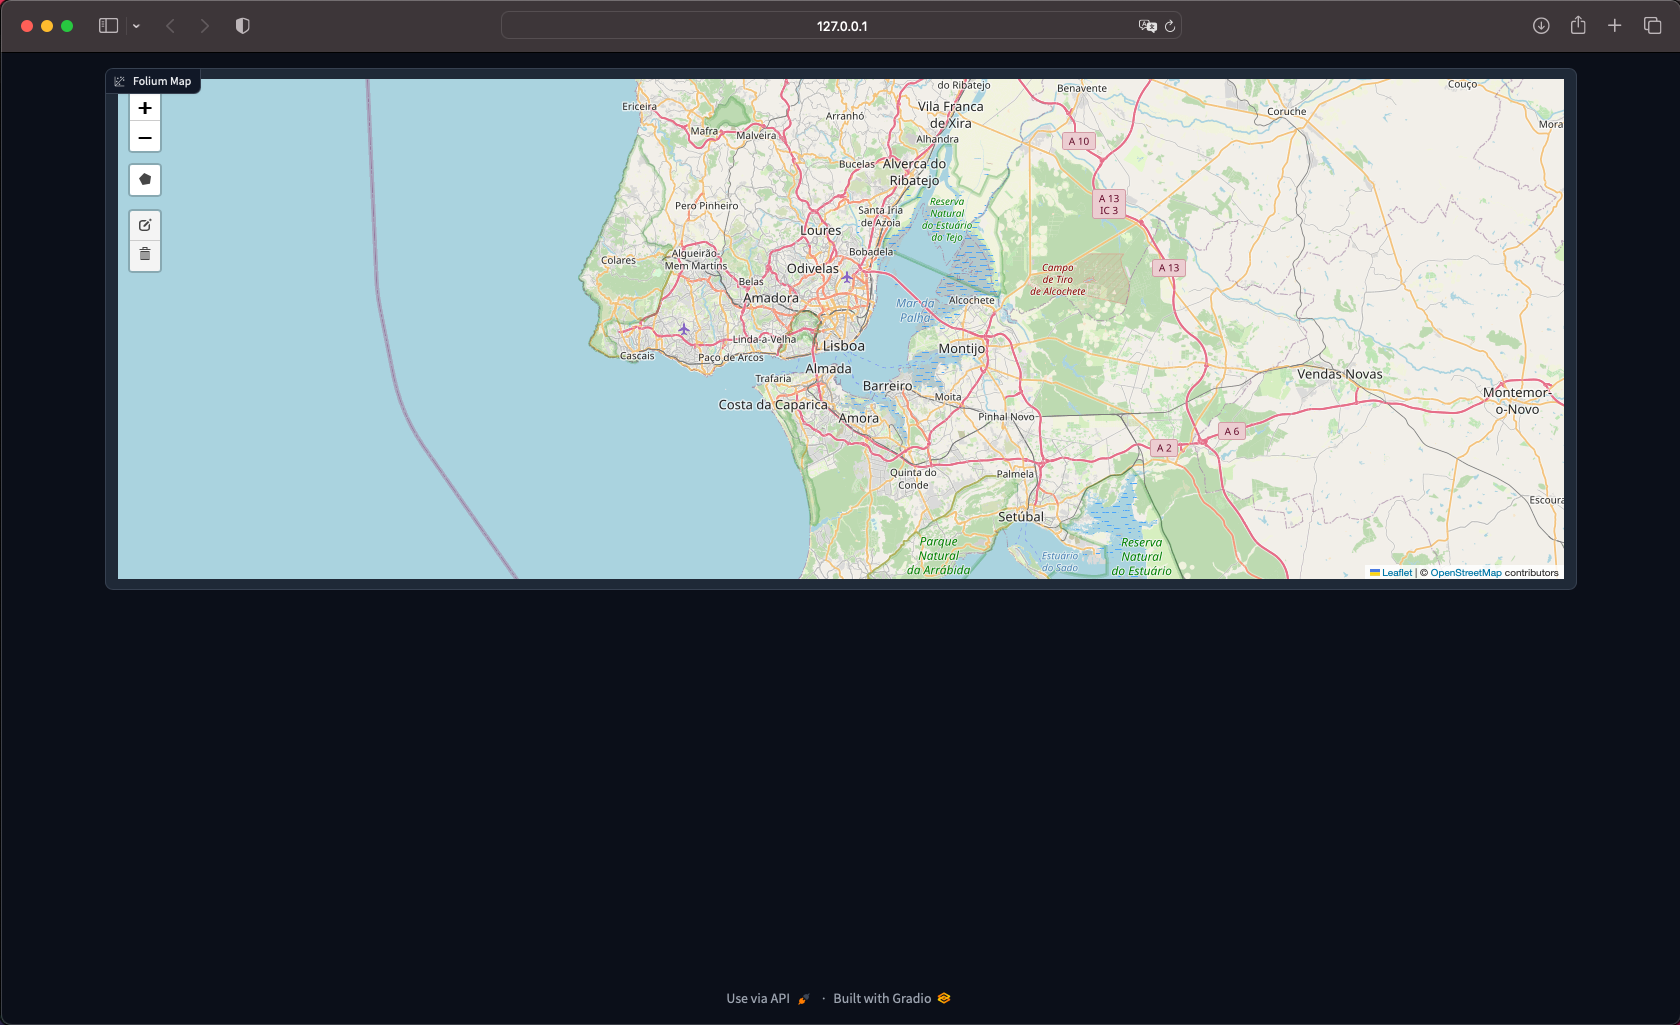
\includegraphics[width=14cm]{ss11.5.png}
\caption{Map Starting at a Random City}\label{fig:ss11.5}
\end{figure}

\begin{center}
\csvloop{
    file=data/minitests.csv,
    no head,
    column count=6,
    column names={1=\mtestID, 2=\mtestName, 3=\mtestInputs, 4=\mtestType, 5=\mtestExpectedOutputs, 6=\mtestRealOutputs},
    filter ifthen={\equal{\mtestID}{$t_{48}$}\OR\equal{\mtestID}{\textbf{No.}}},
    before reading={
        \begin{longtable}{|m{1cm}|m{3cm}|m{3cm}|m{2cm}|m{3cm}|m{3cm}|}
        \hline
    },
    command=\csvlinetotablerow,
    late after line=\\\hline,
    after reading={
        \caption{Testing Table for Code Snippet \ref{cs:randomCity}}
        \end{longtable}
    }
}
\end{center}

Now I need to retrieve the region the user draws on the map, in order to process it and make predictions. I did not know how to do this, so I began to research the problem.

After looking through many forums and StackOverflow pages, it seems that accessing the region drawn in the folium map dynamically is impossible.

\begin{listing}[H]
\pil{app.py}
\begin{minted}[linenos,breaklines,frame=single,firstnumber=13]{python}
    export=True,
    filename='region.geojson',
\end{minted}
\pil{app.py}
\begin{minted}[linenos,breaklines,frame=single,firstnumber=28]{python}
# structure of the UI
with gr.Blocks() as app:
    map = Folium(value=foliumMap)
    uploadButton = gr.UploadButton(label='Upload the GeoJSON file', file_count='single')
\end{minted}
\caption{Reading the Map for the Region}\label{cs:readingMapForRegion}
\end{listing}

Instead, I have decided to set the \pil{export} attribute (in \pil{Draw}) to \pil{True}, meaning that there will now be an export button on the top right of the map. This will download a \pil{.geojson} file to the user's computer containing the region.

The user can then upload their \pil{.geojson} file to be read and processed.

\begin{figure}[H]
\centering
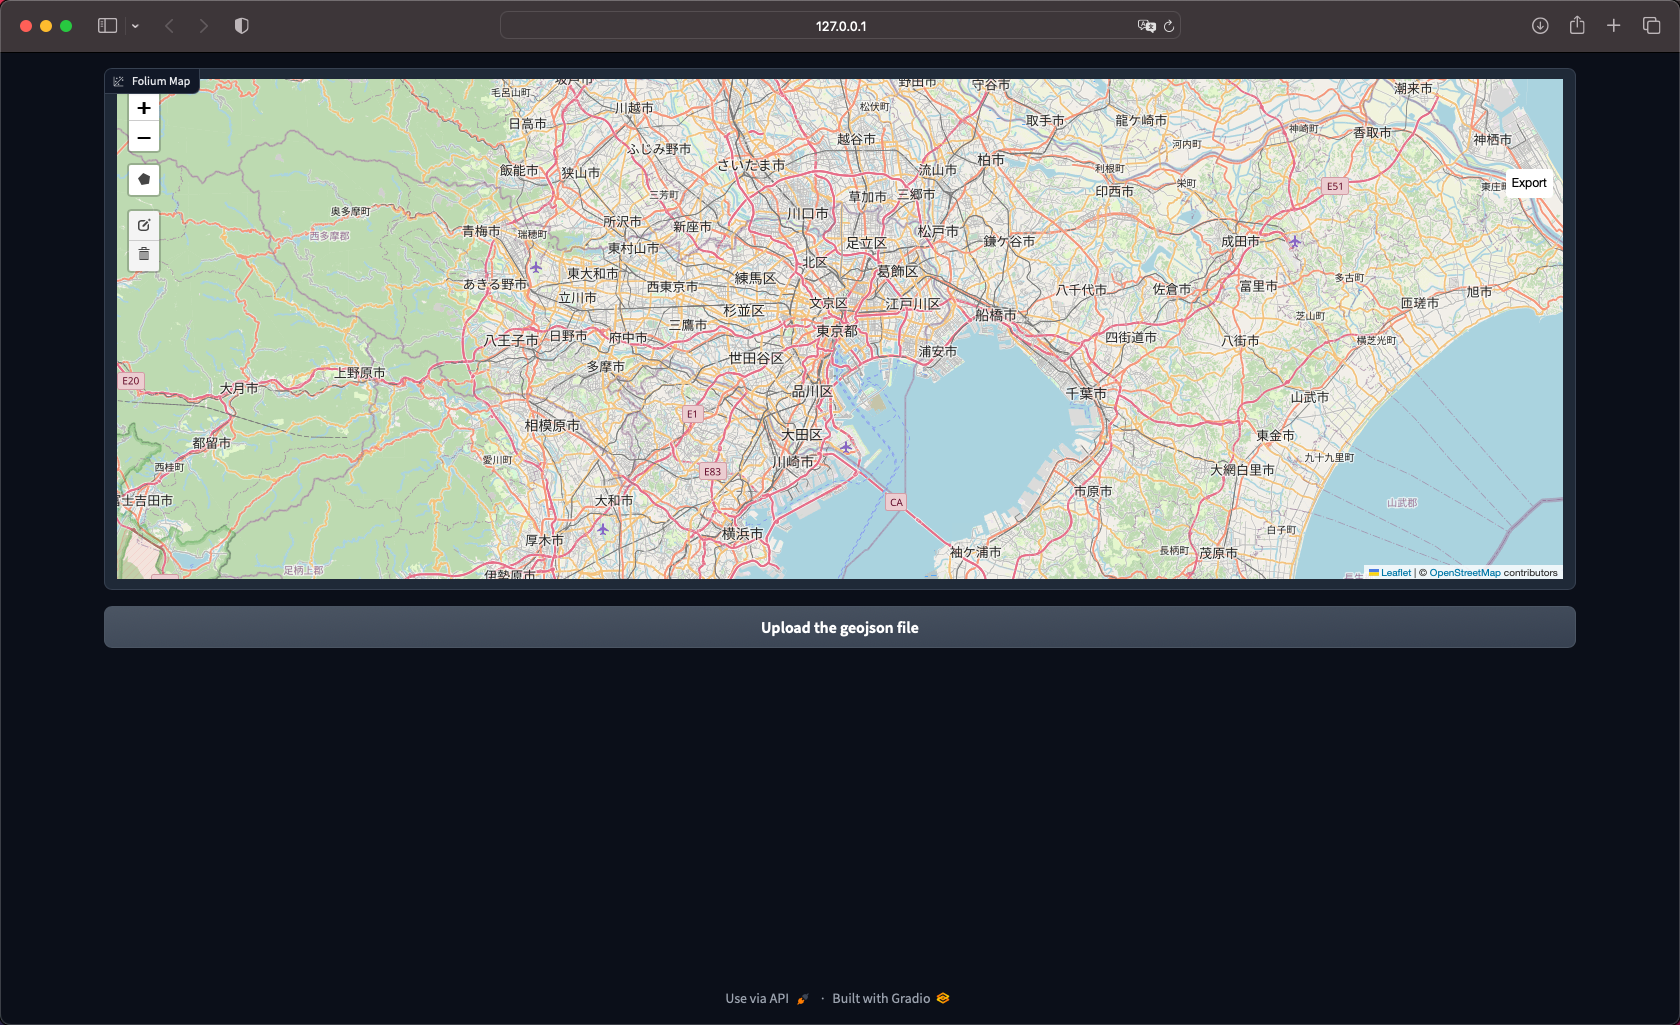
\includegraphics[width=14cm]{ss11.6.png}
\caption{Upload Button Added}\label{fig:ss11.6}
\end{figure}

Figure \ref{fig:ss11.6} shows the output with these new changes. This is not an ideal solution, as the way the user uses the main function of the app has become a bit cumbersome. However, I cannot see a way around this, for now at least.

\begin{center}
\csvloop{
    file=data/minitests.csv,
    no head,
    column count=6,
    column names={1=\mtestID, 2=\mtestName, 3=\mtestInputs, 4=\mtestType, 5=\mtestExpectedOutputs, 6=\mtestRealOutputs},
    filter ifthen={\equal{\mtestID}{$t_{49}$}\OR\equal{\mtestID}{\textbf{No.}}},
    before reading={
        \begin{longtable}{|m{1cm}|m{3cm}|m{3cm}|m{2cm}|m{3cm}|m{3cm}|}
        \hline
    },
    command=\csvlinetotablerow,
    late after line=\\\hline,
    after reading={
        \caption{Testing Table for Code Snippet \ref{cs:readingMapForRegion}}
        \end{longtable}
    }
}
\end{center}

The button to export the \pil{.geojson} file does not work and will be implemented in the next part.

\stepcounter{parts}
\subsection{Part \theparts{} -- Predicting the HDI}

\begin{listing}[H]
\pil{app.py}
\begin{minted}[linenos,breaklines,frame=single,firstnumber=32]{python}
    log = gr.Textbox(label='Log Messages', value='', interactive=False)
\end{minted}
\caption{Adding a Log Textbox}\label{cs:logTextbox}
\end{listing}

I first wanted to add a Log Textbox to the GUI, which will show messages when executing operations successfully. For this, we can use the gradio \pil{Textbox}, with the \pil{interactice} argument set to \pil{False}. This will make it so that the user cannot write in the text box.

This was added below the other elements, and should appear below them on the screen.

\begin{figure}[H]
\centering
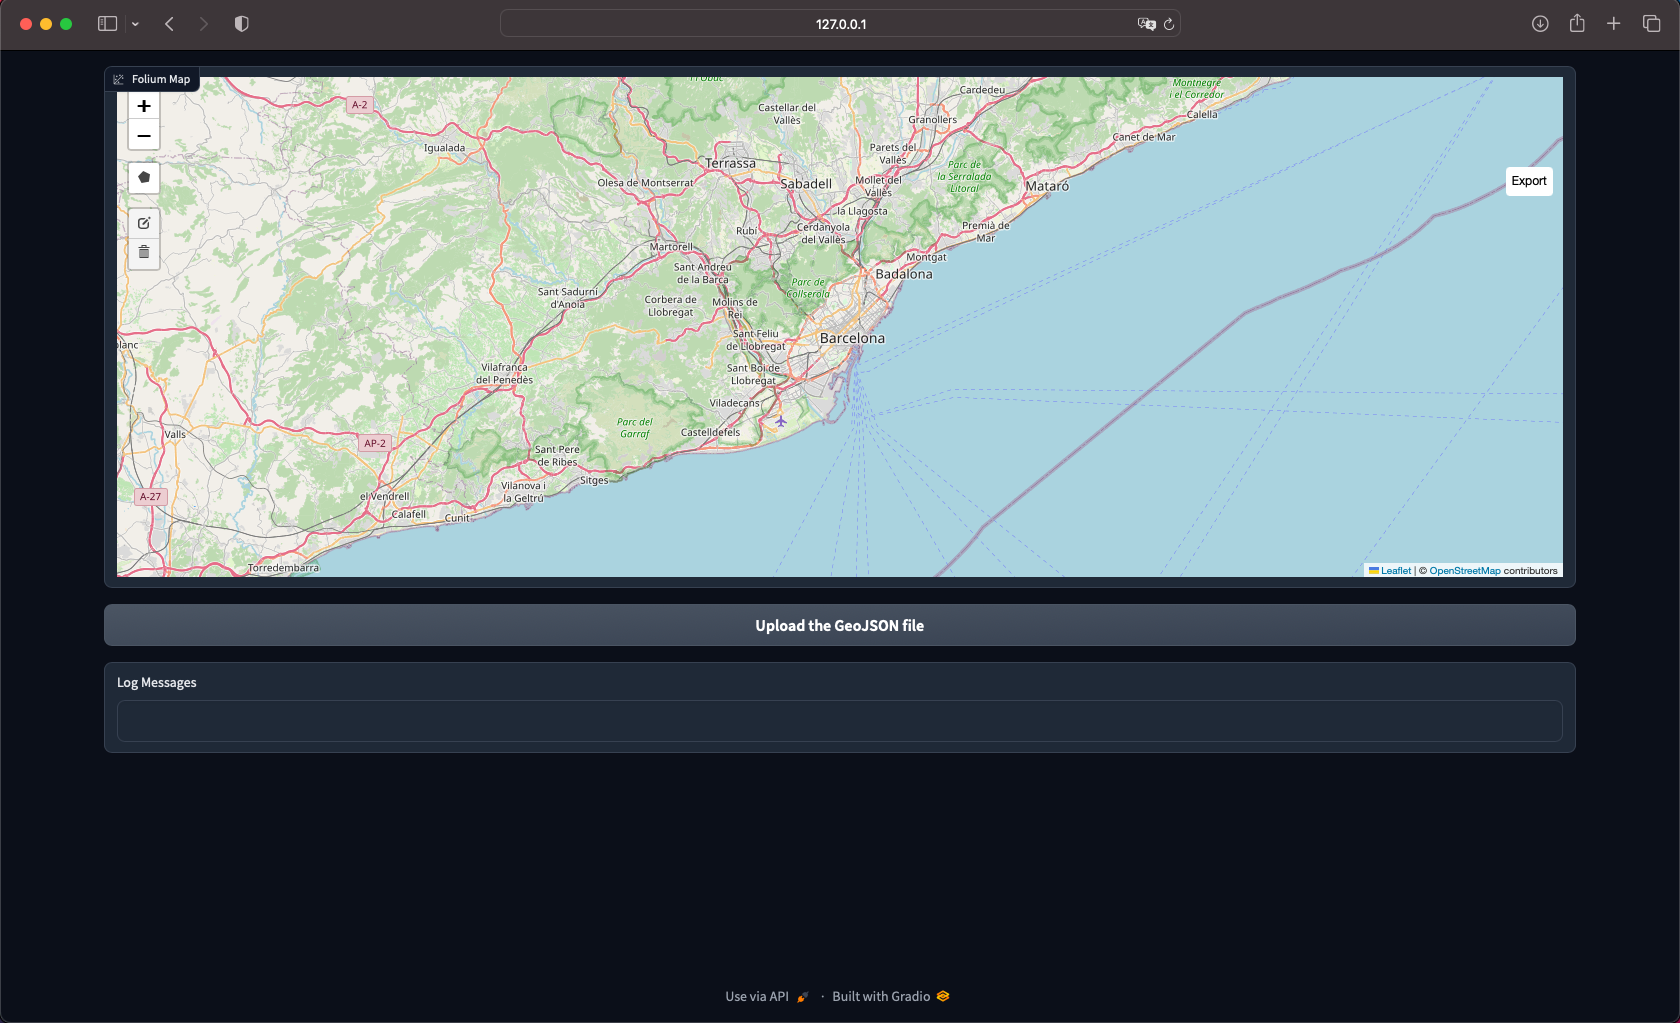
\includegraphics[width=14cm]{ss12.1.png}
\caption{Log Textbox Added}\label{fig:ss12.1}
\end{figure}

\begin{center}
\csvloop{
    file=data/minitests.csv,
    no head,
    column count=6,
    column names={1=\mtestID, 2=\mtestName, 3=\mtestInputs, 4=\mtestType, 5=\mtestExpectedOutputs, 6=\mtestRealOutputs},
    filter ifthen={\equal{\mtestID}{$t_{50}$}\OR\equal{\mtestID}{\textbf{No.}}},
    before reading={
        \begin{longtable}{|m{1cm}|m{3cm}|m{3cm}|m{2cm}|m{3cm}|m{3cm}|}
        \hline
    },
    command=\csvlinetotablerow,
    late after line=\\\hline,
    after reading={
        \caption{Testing Table for Code Snippet \ref{cs:logTextbox}}
        \end{longtable}
    }
}
\end{center}

Now we must add functionality to the upload button.

\begin{listing}[H]
\pil{app.py}
\begin{minted}[linenos,breaklines,frame=single,firstnumber=6]{python}
import json

# define global vars
currentRegion = []

# code to process the user uploading their geojson file
def uploadGeoJSON(filename):
    global currentRegion
    with open(filename, 'r') as file:
        data = json.load(file)
        currentRegion = [coordinate[::-1] for coordinate in data['features'][0]['geometry']['coordinates'][0]]
    return f'Successfully Uploaded {filename[filename.rindex("/")+1:]}'

\end{minted}
\pil{app.py}
\begin{minted}[linenos,breaklines,frame=single,firstnumber=46]{python}
    # functionality
    uploadButton.upload(uploadGeoJSON, inputs=[uploadButton], outputs=[log])
\end{minted}
\caption{Adding Functionality to the Upload Button}\label{cs:uploadButtonFunctionality}
\end{listing}

All of the functionalities in the gradio interface will be of the format: \pil{component.action( function, inputs=[...], outputs=[...])}, where the inputs and outputs are lists of components, and still contained within the \pil{with gr.Blocks()} statement. Therefore, the code to make the upload button interactive is that shown on line 47, where \pil{uploadGeoJSON} is the identifier of some function.

To store the current region, we can use a \pil{global} variable, \pil{currentRegion}. Recalling how \pil{.geojson} files are structured, to get the coordinates into the right format, we must reverse each coordinate before storing it.

Once we have read the contents of the uploaded file, we can return a string to be displayed in the log textbox. The filename given by the parameter will be its full path, so we only want to take a substring of that starting with the character after the last \pil{'/'}.

\begin{figure}[H]
\centering
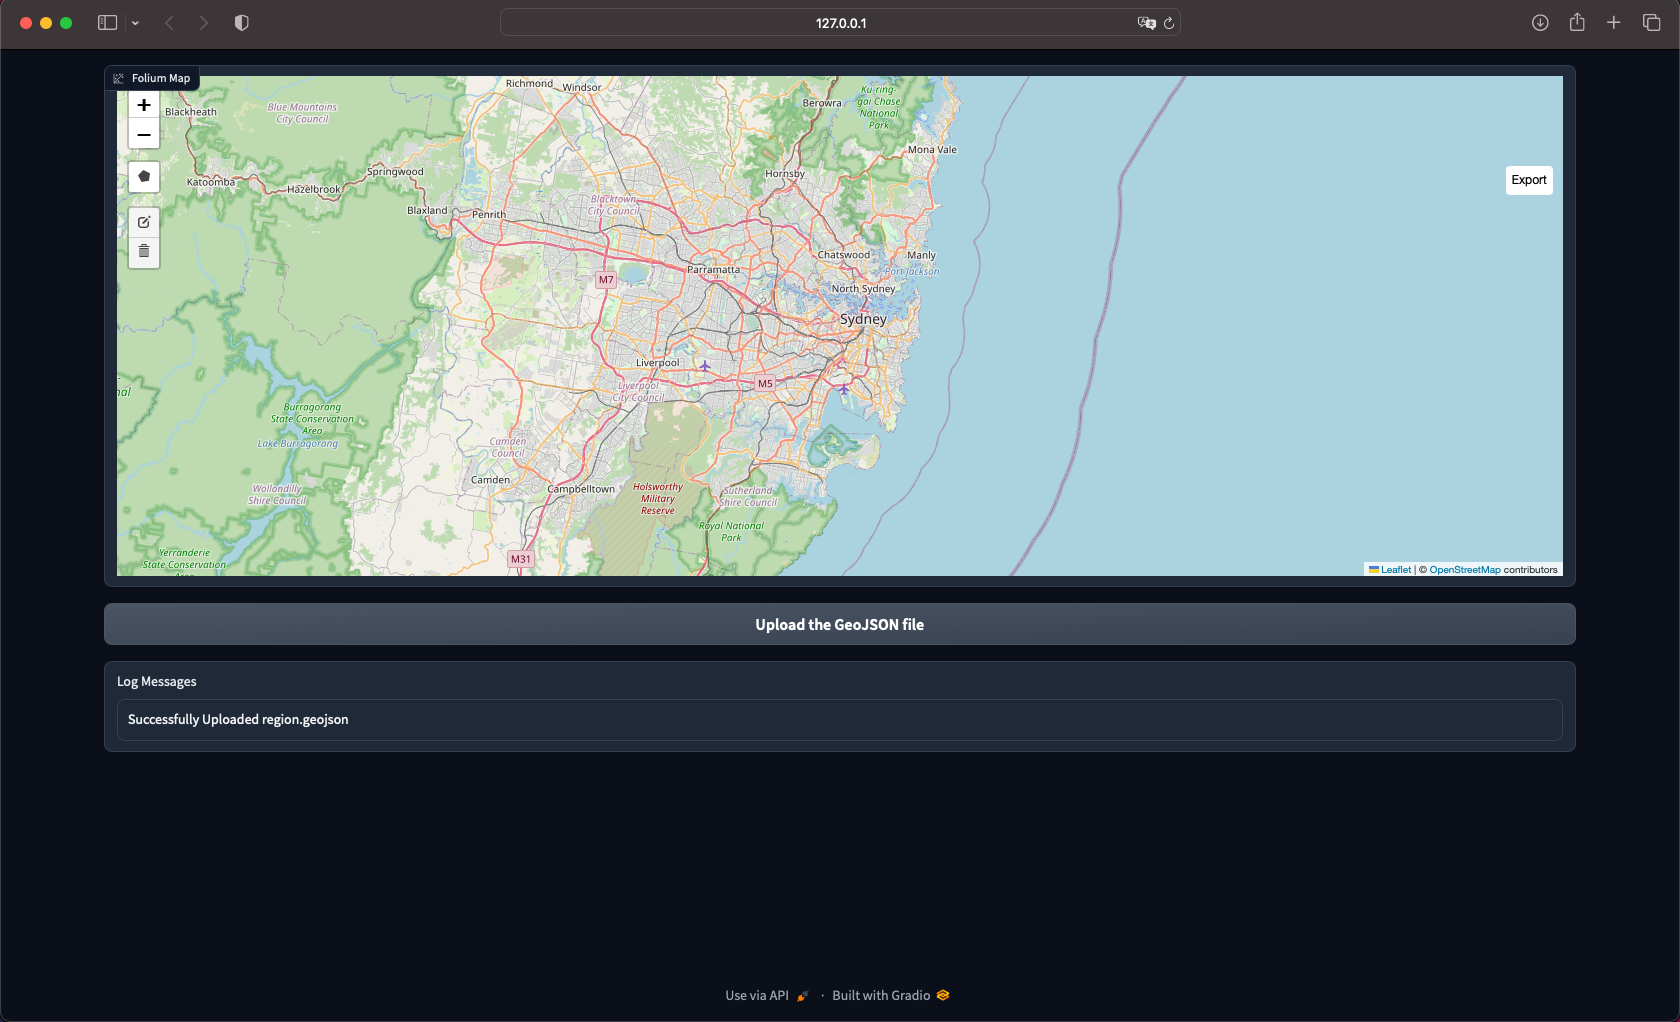
\includegraphics[width=14cm]{ss12.2.png}
\caption{Uploading GeoJSON Files}\label{fig:ss12.2}
\end{figure}

\begin{center}
\csvloop{
    file=data/minitests.csv,
    no head,
    column count=6,
    column names={1=\mtestID, 2=\mtestName, 3=\mtestInputs, 4=\mtestType, 5=\mtestExpectedOutputs, 6=\mtestRealOutputs},
    filter ifthen={\equal{\mtestID}{$t_{51}$}\OR\equal{\mtestID}{\textbf{No.}}},
    before reading={
        \begin{longtable}{|m{1cm}|m{3cm}|m{3cm}|m{2cm}|m{3cm}|m{3cm}|}
        \hline
    },
    command=\csvlinetotablerow,
    late after line=\\\hline,
    after reading={
        \caption{Testing Table for Code Snippet \ref{cs:uploadButtonFunctionality}}
        \end{longtable}
    }
}
\end{center}

\begin{listing}[H]
\pil{app.py}
\begin{minted}[linenos,breaklines,frame=single,firstnumber=40]{python}
# structure of the UI
with gr.Blocks() as app:
    with gr.Row():
        with gr.Column(scale=3):
            map = Folium(value=foliumMap)
            uploadButton = gr.UploadButton(label='Upload the GeoJSON file', file_count='single')
        with gr.Column(scale=1):
            predictHDIbutton = gr.Button(value='Predict HDI', variant='primary')
            HDIprediction = gr.Textbox(label='I believe that the HDI of this region is...', value='', interactive=False)
    log = gr.Textbox(label='Log Messages', value='', interactive=False)
\end{minted}
\caption{Placing the Predict Button}\label{cs:placePredict}
\end{listing}

In order to place the prediction button as shown by the Interface Sketch (Figure \ref{fig:interfaceSketch1}), we must make use of gradio \pil{Row}s and \pil{Column}s.

As we want out map and upload button to be arranged vertically, we can place them in a \pil{Column}. The same goes fro the button to predict HDI and the output textbox for the HDI prediction. As we want these two columns to be arranged side by side, we can put them in a \pil{Row}. As the log textbox should be below everything, it should be placed outside of the \pil{Row}. In my opinion, this use of context managers (\pil{with gr.Row()} and \pil{with gr.Column()}) makes the code extremely readable, and easy to understand where elements will end up.

If we want the width of the first column (containing the map) to be larger than the width of the second, we can use the \pil{scale} attribute, to specify the ratio of the widths. Here, I have specified that the width of the map column should be 3 times the width of the prediciton column.

For the actual button, setting the \pil{variant} attribute to \pil{'primary'} makes the button appear in the primary colour of the app, which is orange.

\begin{figure}[H]
\centering
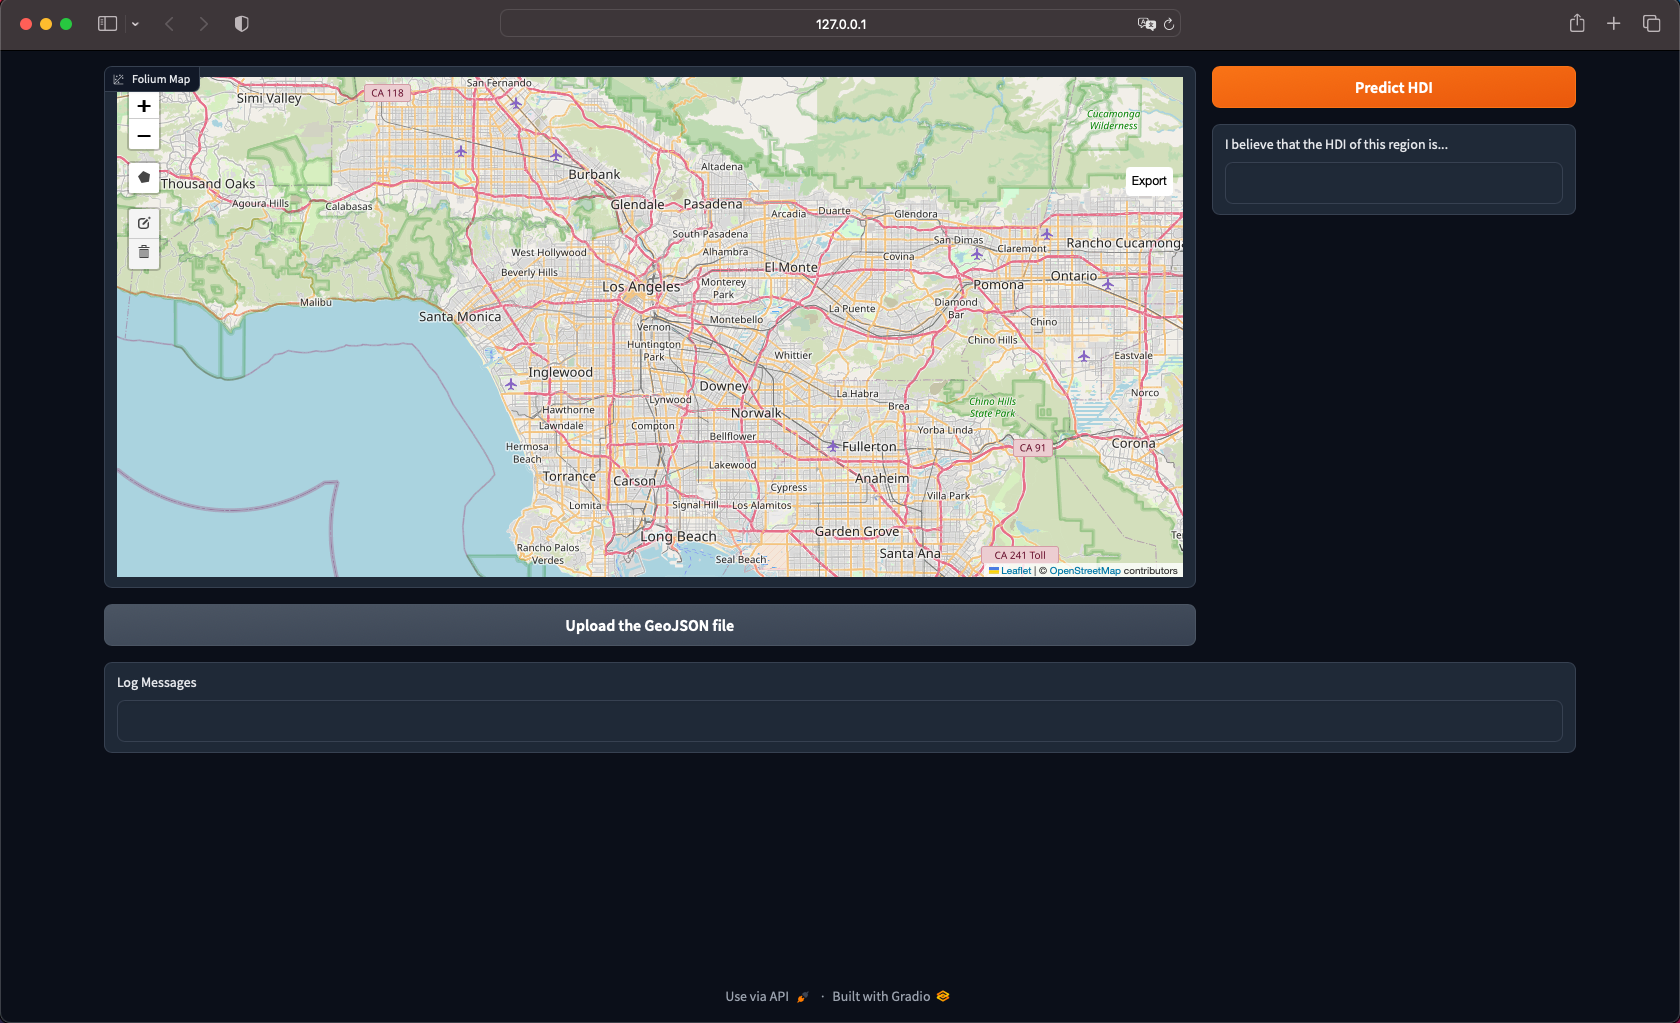
\includegraphics[width=14cm]{ss12.3.png}
\caption{New Structure of the GUI}\label{fig:ss12.3}
\end{figure}

\begin{center}
\csvloop{
    file=data/minitests.csv,
    no head,
    column count=6,
    column names={1=\mtestID, 2=\mtestName, 3=\mtestInputs, 4=\mtestType, 5=\mtestExpectedOutputs, 6=\mtestRealOutputs},
    filter ifthen={\equal{\mtestID}{$t_{52}$}\OR\equal{\mtestID}{\textbf{No.}}},
    before reading={
        \begin{longtable}{|m{1cm}|m{3cm}|m{3cm}|m{2cm}|m{3cm}|m{3cm}|}
        \hline
    },
    command=\csvlinetotablerow,
    late after line=\\\hline,
    after reading={
        \caption{Testing Table for Code Snippet \ref{cs:placePredict}}
        \end{longtable}
    }
}
\end{center}

Now it is time to implement the functionality of the predict HDI button.

\begin{listing}[H]
\pil{app.py}
\begin{minted}[linenos,breaklines,frame=single,firstnumber=19]{python}
# predict the HDI of the given region
def processPrediction(progress=gr.Progress()):
    global currentRegion
    if currentRegion == []:
        return 'You have not uploaded a region!'
    progress(0, desc='Starting...')
\end{minted}
\caption{Processing the Prediction}\label{cs:processPrediction}
\end{listing}

Again, we must define a funciton, to pass into the gradio interface, which will carry out the required processes.

We must first determine if the user had in fact uploaded a region. If they haven't, it will still be an empty \pil{list}, and so we should return an error message before any calculations are carried out.

I imagine this function will take a lot of time to run, and so I would like for it to show a progress bar to the user. We can do this by using a \pil{gr.Progress()} bar. This allows us to set the progress bar to different percentages at different times within the function (as shown on line 24).

The rest of this function will be very similar to stuff we have written before, mainly \pil{def getAllFactors}, with some small changes.

\begin{listing}[H]
\pil{app.py}
\begin{minted}[linenos,breaklines,frame=single,firstnumber=7]{python}
from data_processing.get_osm_data import get_osm_data
\end{minted}
\pil{app.py}
\begin{minted}[linenos,breaklines,frame=single,firstnumber=11]{python}
all_objects = {}
\end{minted}
\pil{app.py / def processPrediction}
\begin{minted}[linenos,breaklines,frame=single,firstnumber=23]{python}
    global all_objects
\end{minted}
\pil{app.py / def processPrediction}
\begin{minted}[linenos,breaklines,frame=single,firstnumber=27]{python}
    # retrieve all relevant osm data
    object_types = ['house', 'school', 'hospital', 'pharmacy', 'restaurant', 'place_of_worship', 'bank', 'slot_machines', 'fast_food', 'toilets', 'police', 'university', 'library', 'post_box', 'vending_machine', 'bench', 'tree']
    all_objects = {}
    for num, object_type in enumerate(object_types):
        progress(0.3*(num/len(object_types)), desc=f'Downloading {object_type} data...')
        print(f'getting {object_type} data...') # log message
        all_objects[object_type] = get_osm_data(object_type, currentRegion)
\end{minted}
\caption{Retrieving All Relevant OSM Data}\label{cs:retrieveOSMdata}
\end{listing}

The first thing we must do is download all of the different objects from OpenStreetMaps, by calling the \pil{def get_osm_data} function written in Section \ref{sec:get_osm_data}. We must also initialise a global dictionary to contain all of these objects, as we will need to use them later, to improve the HDI.

Again, we can use the \pil{progress} function to set the length of the progress bar according to how far through the list of object types to download we are.

\begin{center}
\csvloop{
    file=data/minitests.csv,
    no head,
    column count=6,
    column names={1=\mtestID, 2=\mtestName, 3=\mtestInputs, 4=\mtestType, 5=\mtestExpectedOutputs, 6=\mtestRealOutputs},
    filter ifthen={\equal{\mtestID}{$t_{12}$}\OR\equal{\mtestID}{\textbf{No.}}},
    before reading={
        \begin{longtable}{|m{1cm}|m{3cm}|m{3cm}|m{2cm}|m{3cm}|m{3cm}|}
        \hline
    },
    command=\csvlinetotablerow,
    late after line=\\\hline,
    after reading={
        \caption{Testing Table for Code Snippets \ref{cs:processPrediction} \& \ref{cs:retrieveOSMdata}}
        \end{longtable}
    }
}
\end{center}

\begin{listing}[H]
\pil{app.py}
\begin{minted}[linenos,breaklines,frame=single,firstnumber=8]{python}
from calc_factors import averageDistance
\end{minted}
\pil{app.py}
\begin{minted}[linenos,breaklines,frame=single,firstnumber=13]{python}
averageDistanceFactors = [['house', 'school'], ['house', 'hospital'], ['house', 'pharmacy'], ['house', 'restaurant'], ['school', 'hospital'], ['police', 'hospital'], ['house', 'place_of_worship'], ['bank', 'slot_machines'], ['fast_food', 'toilets'], ['house', 'police'], ['university', 'library'], ['house', 'library']]
\end{minted}
\pil{app.py / def processPrediction}
\begin{minted}[linenos,breaklines,frame=single,firstnumber=36]{python}
    # calculate average distances
    allFactors = []
    for num, averageDistanceFactor in enumerate(averageDistanceFactors):
        progress(0.3+0.6*(num/len(averageDistanceFactors)), desc=f'Calculating Average Distance between {averageDistanceFactor[0]} and {averageDistanceFactor[1]}...')
        print(f'finding A({averageDistanceFactor[0]}, {averageDistanceFactor[1]})...') # log message
        allFactors.append(averageDistance( all_objects[averageDistanceFactor[0]], all_objects[averageDistanceFactor[1]]))
\end{minted}
\caption{Calculating $A\left(x,y\right)$ Factors}\label{cs:predictionAverageDistance}
\end{listing}

Next, we must calculate each of the average distance factors. I have defined a \pil{list} of the pairs of each object type, and so they can just be fed into the function to calculate the average distance. We can again use the \pil{progress()} function to update the progress bar.

At this point, I decided to make a copy of the \pil{calc_factors.py} file, and placed it in the main directory, instead of the \pil{data_processing} directory. This is because I plan to make small edits to how some of these functions are going to work.

\begin{listing}[H]
\pil{app.py}
\begin{minted}[linenos,breaklines,frame=single,firstnumber=8]{python}
from calc_factors import averageDistance, calcArea, density
\end{minted}
\pil{app.py}
\begin{minted}[linenos,breaklines,frame=single,firstnumber=14]{python}
densityFactors = ['school', 'hospital', 'pharmacy', 'police', 'library', 'toilets', 'restaurant', 'place_of_worship', 'post_box', 'vending_machine', 'bench', 'tree']
\end{minted}
\pil{app.py / def processPrediction}
\begin{minted}[linenos,breaklines,frame=single,firstnumber=43]{python}
    # calculate area
    progress(0.9, desc='Calculating Area...')
    print('calculating area...') # log message
    area = calcArea(currentRegion)
    # calculate density factors
    for num, densityFactor in enumerate(densityFactors):
        progress(0.91+0.05*(num/len(densityFactors)), desc=f'Calculating {densityFactor} Density...')
        print(f'finding D({densityFactor})') # log message
        allFactors.append(density(all_objects[densityFactor], area))
\end{minted}
\caption{Calculating $D\left(x\right)$ Factors}\label{cs:predictionDensity}
\end{listing}

We can also calculate the density factors in a similar way, by defining a \pil{list} of all the factors, and iterating over them. We must first however calculate the area of the region, to pass into the \pil{def density} function.

\begin{center}
\csvloop{
    file=data/minitests.csv,
    no head,
    column count=6,
    column names={1=\mtestID, 2=\mtestName, 3=\mtestInputs, 4=\mtestType, 5=\mtestExpectedOutputs, 6=\mtestRealOutputs},
    filter ifthen={\equal{\mtestID}{$t_{13}$}\OR\equal{\mtestID}{\textbf{No.}}},
    before reading={
        \begin{longtable}{|m{1cm}|m{3cm}|m{3cm}|m{2cm}|m{3cm}|m{3cm}|}
        \hline
    },
    command=\csvlinetotablerow,
    late after line=\\\hline,
    after reading={
        \caption{Testing Table for Code Snippets \ref{cs:predictionAverageDistance} \& \ref{cs:predictionDensity}}
        \end{longtable}
    }
}
\end{center}

Now that we have a full list of factors, we can predict the HDI

\begin{listing}[H]
\pil{app.py}
\begin{minted}[linenos,breaklines,frame=single,firstnumber=9]{python}
import numpy as np
from neural_network import MultilayerPerceptron

# initialise neural network
network = MultilayerPerceptron([24, 18, 12, 6, 3, 1])
network.load_model('models/hdi.pkl')
\end{minted}
\pil{app.py / def processPrediction}
\begin{minted}[linenos,breaklines,frame=single,firstnumber=58]{python}
    # predict HDI
    progress(0.96, desc='Predicting HDI...')
    inputLayer = np.matrix([[100 if factor == None else float(factor)/10 if index <= 11 else float(factor)] for index, factor in enumerate(allFactors)])
    prediction = round(network.predict(inputLayer).item(0,0), 3)
    return prediction
\end{minted}
\caption{Predicting the HDI}\label{cs:predictingHDI}
\end{listing}

For this, we must first import the \pil{MultilayerPerceptron} from \pil{neural_network.py}, and set the layer sizes to the right values. We can then use the \pil{load_model} method to load the model we trained in Section \ref{sec:trainNetwork}.

Then, at the end of the \pil{def processPrediction} function, we can get a matrix for the input layer (dividing the average distance factors by 10 in the same way as done before), and then we can make a prediction, to be returned. 

\begin{listing}[H]
\pil{app.py / def processPrediction}
\begin{minted}[linenos,breaklines,frame=single,firstnumber=99]{python}
    predictHDIbutton.click(processPrediction, inputs=[], outputs=[HDIprediction])
\end{minted}
\caption{Adding Functionality to the Prediction Button}\label{cs:predictionButton}
\end{listing}

To make the button actually work, we must add a gradio functionality. This line of code makes it so that when the \pil{predictHDIbutton} is \pil{click}ed, it calles the \pil{processPrediction} function, passing in no inputs (as the region is already a global variable), and outputting to the \pil{HDIprediction} textbox.

\begin{figure}[H]
\centering
\includegraphics[width=12cm]{ss12.4.png}
\caption{Progress Bar}\label{fig:ss12.4}
\end{figure}

Figure \ref{fig:ss12.4} shows the progress bar as the prediction is taking place. Gradio, by default, also provides a timer for these processes (as shown in the top right).

\begin{figure}[H]
\centering
\includegraphics[width=14cm]{ss12.5.png}
\caption{Successful Prediction from a Region}\label{fig:ss12.5}
\end{figure}

Figure \ref{fig:ss12.5} shows the prediction for Oxford, which is pretty close.

\begin{center}
\csvloop{
    file=data/minitests.csv,
    no head,
    column count=6,
    column names={1=\mtestID, 2=\mtestName, 3=\mtestInputs, 4=\mtestType, 5=\mtestExpectedOutputs, 6=\mtestRealOutputs},
    filter ifthen={\equal{\mtestID}{$T_{6.1}$}\OR\equal{\mtestID}{$T_{6.2}$}\OR\equal{\mtestID}{$T_{6.3}$}\OR\equal{\mtestID}{\textbf{No.}}},
    before reading={
        \begin{longtable}{|m{1cm}|m{3cm}|m{3cm}|m{2cm}|m{3cm}|m{3cm}|}
        \hline
    },
    command=\csvlinetotablerow,
    late after line=\\\hline,
    after reading={
        \caption{$T_{6}$ Testing Table (for Code Snippets \ref{cs:predictingHDI} \& \ref{cs:predictionButton})}
        \end{longtable}
    }
}
\end{center}

Unfortunately however, this took about 9 minutes to fully complete, which is too much time to wait. By looking at the progress bar, I found that the majority of the time taken was spent in calculating the average distance factors. Therefore, I plan to let the user change the \pil{max_x_objects} variable with a slider, along with a new \pil{max_y_objects} variable, which must first be implemented.

\begin{listing}[H]
\pil{calc_factors.py}
\begin{minted}[linenos,breaklines,frame=single,firstnumber=18]{python}
# finds the average distance between 2 types of objects, A(x,y)
def averageDistance(x_objects, y_objects, max_x_objects=2000, max_y_objects=2000):
\end{minted}
\pil{calc_factors.py / def averageDistance}
\begin{minted}[linenos,breaklines,frame=single,firstnumber=58]{python}
        if len(y_objects) > max_y_objects:
            y_objects_in_consideration = random.sample(y_objects, max_y_objects)
        else:
            y_objects_in_consideration = y_objects
        for y_object in y_objects_in_consideration:
            dist_to_ys.append(distBetween2Points(x_object, y_object))
\end{minted}
\caption{Implementing a Maximum for $y$-objects}\label{cs:maxYobjects}
\end{listing}

In the \pil{def averageDistance} function (in the new \pil{calc_factors.py} file), we can pass in \pil{max_y_objects} in as a parameter, with a default value of 2000. When we iterate for each \pil{x_object}, we can random sample the \pil{y_objects} if nescessary.

This means that we are no longer finding the absolute Average Shortest Distance from $x$ to $y$, as the $y$-objects we select may not include the closest one to the current $x$-object. However, this may actually make the metric more realistic, for a reason which is best shown with an example. The closest school to my house is my primary school, which I no longer attend. Therefore, when I travel to school, I must travel further than the distance from my house to the closest school. This would be reflected in the code by the fact that my primary school may not be selected in the random sample of all the schools ($y$-objects in this example).

\begin{center}
\csvloop{
    file=data/minitests.csv,
    no head,
    column count=6,
    column names={1=\mtestID, 2=\mtestName, 3=\mtestInputs, 4=\mtestType, 5=\mtestExpectedOutputs, 6=\mtestRealOutputs},
    filter ifthen={\equal{\mtestID}{$t_{53}$}\OR\equal{\mtestID}{\textbf{No.}}},
    before reading={
        \begin{longtable}{|m{1cm}|m{3cm}|m{3cm}|m{2cm}|m{3cm}|m{3cm}|}
        \hline
    },
    command=\csvlinetotablerow,
    late after line=\\\hline,
    after reading={
        \caption{Testing Table for Code Snippet \ref{cs:maxYobjects}}
        \end{longtable}
    }
}
\end{center}

\begin{listing}[H]
\pil{app.py}
\begin{minted}[linenos,breaklines,frame=single,firstnumber=28]{python}
# predict the HDI of the given region
def processPrediction(max_x_objects, max_y_objects, progress=gr.Progress()):
\end{minted}
\pil{app.py / def processPrediction}
\begin{minted}[linenos,breaklines,frame=single,firstnumber=48]{python}
        allFactors.append(averageDistance( all_objects[averageDistanceFactor[0]], all_objects[averageDistanceFactor[1]], max_x_objects, max_y_objects))
\end{minted}
\caption{Passing in the \pil{max_y_objects}}\label{cs:passingMaxYobjects}
\end{listing}

To then take these variables into account when calculating factors, we must pass the \pil{max_x_objects} and \pil{max_y_objects} variables into the \pil{def processPrediction} function.

Then, inside that function, we must pass them into the the \pil{def averageDistance} function.

\begin{listing}[H]
\pil{app.py}
\begin{minted}[linenos,breaklines,frame=single,firstnumber=93]{python}
            predictHDIbutton = gr.Button(value='Predict HDI', variant='primary')
            with gr.Group():
                max_x_objectsSlider = gr.Slider(minimum=10, maximum=5000, value=500, label='Maximum x-buildings', info='When calculating the average distance between 2 types of building, it will find the average of this many pairs. Increasing this value may make the prediction take much longer, but may make the prediction more acurate.')
                max_y_objectsSlider = gr.Slider(minimum=10, maximum=5000, value=500, label='Maximum y-buildings', info='When calculating the average distance between 2 types of building, it will find the closest of the second type of building out of this many options. Increasing this value may make the prediction take much longer, but may make the prediction more acurate.')
            with gr.Group():
                HDIprediction = gr.Textbox(label='I believe that the HDI of this region is...', value='', interactive=False)
                similarHDI = gr.Textbox(label='That\'s a similar HDI to...', value='', interactive=False)
\end{minted}
\caption{Adding Sliders}\label{cs:addSliders}
\end{listing}

To let the user decide the values for \pil{max_x_objects} and \pil{max_y_objects}, we can add some sliders. For each of them, I have set the minimum value to 10 and the maximum value to 5000, with a default value of 500. They also each come with an information label, as their function may not be clear to the user.

The use of the \pil{gr.Group()} block will place these elements together, as shown in Figure \ref{fig:ss12.6}. I have also added an output textbox for the similar HDI region, but I will not be implementing this until the \nth{2} prototype.

\begin{figure}[H]
\centering
\includegraphics[width=14cm]{ss12.6.png}
\caption{\pil{max_x_objects} and \pil{max_y_objects} Sliders}\label{fig:ss12.6}
\end{figure}

\begin{listing}[H]
\pil{app.py}
\begin{minted}[linenos,breaklines,frame=single,firstnumber=104]{python}
    predictHDIbutton.click(processPrediction, inputs=[max_x_objectsSlider, max_y_objectsSlider], outputs=[HDIprediction])
\end{minted}
\caption{Updating Functionality for Predicting HDI Button}\label{cs:addNewInputsToButton}
\end{listing}

To take these slider values into account, we must now pass them as inputs to the \pil{predictHDIbutton.click} method.

\begin{figure}[H]
\centering
\includegraphics[width=14cm]{ss12.7.png}
\caption{Prediction with lower \pil{max_x_objects} and \pil{max_y_objects} values}\label{fig:ss12.7}
\end{figure}

\begin{center}
\csvloop{
    file=data/minitests.csv,
    no head,
    column count=6,
    column names={1=\mtestID, 2=\mtestName, 3=\mtestInputs, 4=\mtestType, 5=\mtestExpectedOutputs, 6=\mtestRealOutputs},
    filter ifthen={\equal{\mtestID}{$t_{54}$}\OR\equal{\mtestID}{\textbf{No.}}},
    before reading={
        \begin{longtable}{|m{1cm}|m{3cm}|m{3cm}|m{2cm}|m{3cm}|m{3cm}|}
        \hline
    },
    command=\csvlinetotablerow,
    late after line=\\\hline,
    after reading={
        \caption{Testing Table for Code Snippets \ref{cs:passingMaxYobjects}, \ref{cs:addSliders} \& \ref{cs:addNewInputsToButton}}
        \end{longtable}
    }
}
\end{center}

This prediction 1 minute instead of 9, 50 seconds of which were spent downloading the locations of all the objects, which I have no control over how long it takes.

\stepcounter{parts}
\subsection{Part \theparts{} -- Suggesting Improvements}

In order to make suggestions, we must first define the inputs and the outputs the user will be interacting with.

\begin{listing}[H]
\pil{app.py}
\begin{minted}[linenos,breaklines,frame=single,firstnumber=100]{python}
    makeSuggestionsButton = gr.Button(value='Make Suggestions')
    suggestionsTable = gr.Dataframe(label='Suggestions', headers=['New Building', 'Coordinates', 'New HDI', 'Change in HDI'], type='array', interactive=False)
\end{minted}
\caption{Adding a Suggestions Table}\label{cs:suggestionsTable}
\end{listing}

Here, I am defining a button in the same way as before, along with a \pil{Dataframe}. This will create a table for us to output to, with headers that we can specify. The \pil{type} of this \pil{Dataframe} is set to \pil{'array'}, as I will be returning a python \pil{list} (as opposed to a \pil{np.ndarray} or similar). To ensure that the user cannot edit the data in each cell, or add new rows and columns, \pil{interactive} has been set to \pil{False}.

\begin{figure}[H]
\centering
\includegraphics[width=14cm]{ss13.1.png}
\caption{Suggestions Table}\label{fig:ss13.1}
\end{figure}

Figure \ref{fig:ss13.1} shows the user interface with these new additions. Unfortunately, there is a small bug in \pil{gradio}, which causes the \pil{Dataframe} to have a small white border for scroll bars, even when they are not required (as in this case). Unfortunately, I cannot do anything about this.

\begin{center}
\csvloop{
    file=data/minitests.csv,
    no head,
    column count=6,
    column names={1=\mtestID, 2=\mtestName, 3=\mtestInputs, 4=\mtestType, 5=\mtestExpectedOutputs, 6=\mtestRealOutputs},
    filter ifthen={\equal{\mtestID}{$t_{55}$}\OR\equal{\mtestID}{\textbf{No.}}},
    before reading={
        \begin{table}[H]
        \centering
        \begin{tabular}{|m{1cm}|m{3cm}|m{3cm}|m{2cm}|m{3cm}|m{3cm}|}
        \hline
    },
    command=\csvlinetotablerow,
    late after line=\\\hline,
    after reading={
        \end{tabular}
        \caption{Testing Table for Code Snippet \ref{cs:suggestionsTable}}
        \end{table}
    }
}
\end{center}

Now we must add functionality to this button.

\begin{listing}[H]
\pil{app.py}
\begin{minted}[linenos,breaklines,frame=single,firstnumber=65]{python}
# make suggestions from a prediction
def makeSuggestions(max_x_objects, max_y_objects, progress=gr.Progress()):
    global all_objects
    suggestions = ['school', 'hospital', 'place_of_worship', 'police', 'restaurant', 'slot_machines', 'library', 'pharmacy']
    returnTable = []
    for num, suggestion in enumerate(suggestions):
        progress(num/len(suggestions), desc=f'Suggesting building a {suggestion}...')
\end{minted}
\caption{Defining the Suggestions Function}\label{cs:suggestionsFunction}
\end{listing}

Here, I am defining the \pil{def makeSuggestions} function, which will be called when the user clicks the make suggestions button. It must take in \pil{max_x_objects} and \pil{max_y_objects} again, as we will be computing average distances. It will also use \pil{gr.Progress} again, as it may take a while.

To avoid downloading all of the objects again, we can use the global variable, \pil{all_objects}, which we saved them to, when predicting the HDI. Then, we must define each of the suggestions, as well as the return list, which will be displayed in the \pil{Dataframe}. We will then iterate over each suggestion and calculate its new HDI (for now however, all we can do is update the progress bar).

\begin{center}
\csvloop{
    file=data/minitests.csv,
    no head,
    column count=6,
    column names={1=\mtestID, 2=\mtestName, 3=\mtestInputs, 4=\mtestType, 5=\mtestExpectedOutputs, 6=\mtestRealOutputs},
    filter ifthen={\equal{\mtestID}{$t_{56}$}\OR\equal{\mtestID}{\textbf{No.}}},
    before reading={
        \begin{longtable}{|m{1cm}|m{3cm}|m{3cm}|m{2cm}|m{3cm}|m{3cm}|}
        \hline
    },
    command=\csvlinetotablerow,
    late after line=\\\hline,
    after reading={
        \caption{Testing Table for Code Snippet \ref{cs:suggestionsFunction}}
        \end{longtable}
    }
}
\end{center}

The first thing we must do for each suggestion is find the optimal place for it to go.

\begin{listing}[H]
\pil{app.py}
\begin{minted}[linenos,breaklines,frame=single,firstnumber=65]{python}
# helper function to calculate mean of coordinates
def calcMeanOfCoords(coords):
    return [np.mean([coord[0] for coord in coords]), np.mean([coord[1] for coord in coords])]
\end{minted}
\caption{Finding the mean of coordinates}\label{cs:meanOfCoordinates}
\end{listing}

To do this, we must be able to calculate the mean of coordinates (that is, the latitude will be the mean of all the latitudes, and the longitude will be the mean of all the longitudes).

\begin{listing}[H]
\pil{app.py}
\begin{minted}[linenos,breaklines,frame=single,firstnumber=69]{python}
# calculate the optimal place for a new building to go when suggesting
def calcOptimalPlaceFor(building):
    global all_objects
    means = []
    for averageDistanceFactor in averageDistanceFactors:
        if averageDistanceFactor[1] == building:
            means.append(calcMeanOfCoords( all_objects[averageDistanceFactor[0]]))
    return calcMeanOfCoords(means)
\end{minted}
\pil{app.py / def makeSuggestions}
\begin{minted}[linenos,breaklines,frame=single,firstnumber=85]{python}
        # find optimal place
        progress((num/len(suggestions))+(0*(1/32)), desc=f'Suggesting building a {suggestion} (finding optimal position)...')
        position = calcOptimalPlaceFor(suggestion)
\end{minted}
\caption{Finding the Optimal Place for a New Building}\label{cs:optimalPlaceForNewBuilding}
\end{listing}

To then find the optimal place (according the the algorithm shown in Figure \ref{fig:newBuilding}), we must iterate over each average distance factor, for which the second parameter is the new building, and find the mean position of the first parameter. The optimal position will then be the mean of those means.

We then must call this function in the actual \pil{def makeSuggestions} function for each of the suggestions.

\begin{center}
\csvloop{
    file=data/minitests.csv,
    no head,
    column count=6,
    column names={1=\mtestID, 2=\mtestName, 3=\mtestInputs, 4=\mtestType, 5=\mtestExpectedOutputs, 6=\mtestRealOutputs},
    filter ifthen={\equal{\mtestID}{$T_{7.1}$}\OR\equal{\mtestID}{$T_{7.2}$}\OR\equal{\mtestID}{$T_{7.3}$}\OR\equal{\mtestID}{\textbf{No.}}},
    before reading={
        \begin{table}[H]
        \centering
        \begin{tabular}{|m{1cm}|m{3cm}|m{3cm}|m{2cm}|m{3cm}|m{3cm}|}
        \hline
    },
    command=\csvlinetotablerow,
    late after line=\\\hline,
    after reading={
        \end{tabular}
        \caption{$T_{7}$ Testing Table (for Code Snippets \ref{cs:meanOfCoordinates} \& \ref{cs:optimalPlaceForNewBuilding})}\label{table:t7testing}
        \end{table}
    }
}
\end{center}

The next step is to calculate the new average distances. As we are making use of random sampling, it would not guaranteed that the new building is considered, if we just add it to the list. Therefore, we must add it to the considered objects after we random sample, which will require some extra parameters:

\begin{listing}[H]
\pil{calc_factors.py}
\begin{minted}[linenos,breaklines,frame=single,firstnumber=18]{python}
# finds the average distance between 2 types of objects, A(x,y)
def averageDistance(x_objects, y_objects, max_x_objects=2000, max_y_objects=2000, must_include_x=None, must_include_y=None):
\end{minted}
\pil{calc_factors.py / def averageDistance}
\begin{minted}[linenos,breaklines,frame=single,firstnumber=24]{python}
    if must_include_x != None: # include the new building when making suggestions
        x_objects[0] = must_include_x
\end{minted}
\pil{calc_factors.py / def averageDistance}
\begin{minted}[linenos,breaklines,frame=single,firstnumber=34]{python}
        if must_include_y != None: # include the new building when making suggestions
            y_objects_in_consideration[0] = must_include_y
\end{minted}
\caption{Updating the Average Distance Function}\label{cs:updateAverageDistance}
\end{listing}

Here, in the \pil{def averageDistance} function, the parameters \pil{must_include_x} and \pil{must_include_y} are set to \pil{None} by default (as to not break the previous function calls). If we pass something in however, we want to include it in the calculations. We can do this by setting the first item in the list to be the new building, as each element in those lists are random ones anyway, so it is irrelevant which one we override.

\begin{listing}[H]
\pil{app.py / def makeSuggestions}
\begin{minted}[linenos,breaklines,frame=single,firstnumber=88]{python}
        # calculate average distances
        progress((num/len(suggestions))+(1*(1/32)), desc=f'Suggesting building a {suggestion} (calculating new average distances)...')
        allFactors = []
        for averageDistanceFactor in averageDistanceFactors:
            # ensure that we include the new building
            if suggestion == averageDistanceFactor[0]:
                allFactors.append(averageDistance( all_objects[averageDistanceFactor[0]], all_objects[averageDistanceFactor[1]], max_x_objects, max_y_objects, must_include_x=position))
            elif suggestion == averageDistanceFactor[1]:
                allFactors.append(averageDistance( all_objects[averageDistanceFactor[0]], all_objects[averageDistanceFactor[1]], max_x_objects, max_y_objects, must_include_y=position))
            else:
                allFactors.append(averageDistance( all_objects[averageDistanceFactor[0]], all_objects[averageDistanceFactor[1]], max_x_objects, max_y_objects))
\end{minted}
\caption{Calculating the New Average Distances}\label{cs:newAverageDistances}
\end{listing}

Then, when we calculate the new average distances, we can pass in the position of the new building as required (either as an \pil{x_object}, \pil{y_object} or neither).

\begin{center}
\csvloop{
    file=data/minitests.csv,
    no head,
    column count=6,
    column names={1=\mtestID, 2=\mtestName, 3=\mtestInputs, 4=\mtestType, 5=\mtestExpectedOutputs, 6=\mtestRealOutputs},
    filter ifthen={\equal{\mtestID}{$t_{57}$}\OR\equal{\mtestID}{\textbf{No.}}},
    before reading={
        \begin{longtable}{|m{1cm}|m{3cm}|m{3cm}|m{2cm}|m{3cm}|m{3cm}|}
        \hline
    },
    command=\csvlinetotablerow,
    late after line=\\\hline,
    after reading={
        \caption{Testing Table for Code Snippets \ref{cs:updateAverageDistance} \& \ref{cs:newAverageDistances}}
        \end{longtable}
    }
}
\end{center}

\begin{listing}[H]
\pil{app.py / def makeSuggestions}
\begin{minted}[linenos,breaklines,frame=single,firstnumber=99]{python}
        # calculate density factors
        progress((num/len(suggestions))+(2*(1/32)), desc=f'Suggesting building a {suggestion} (calculating new densities)...')
        area = calcArea(currentRegion)
        for densityFactor in densityFactors:
            # ensure that we include the new building
            if suggestion == densityFactor:
                allFactors.append(density(all_objects[densityFactor] + [position], area))
            else:
                allFactors.append(density(all_objects[densityFactor], area))
\end{minted}
\caption{Calculating the New Densities}\label{cs:newDensities}
\end{listing}

When calculating the density factors, we must add the position of the new building to the list if and only if the current density factor we are calculating is about the new building. Otherwise, we can just calculate it as normal.

\begin{center}
\csvloop{
    file=data/minitests.csv,
    no head,
    column count=6,
    column names={1=\mtestID, 2=\mtestName, 3=\mtestInputs, 4=\mtestType, 5=\mtestExpectedOutputs, 6=\mtestRealOutputs},
    filter ifthen={\equal{\mtestID}{$t_{58}$}\OR\equal{\mtestID}{\textbf{No.}}},
    before reading={
        \begin{longtable}{|m{1cm}|m{3cm}|m{3cm}|m{2cm}|m{3cm}|m{3cm}|}
        \hline
    },
    command=\csvlinetotablerow,
    late after line=\\\hline,
    after reading={
        \caption{Testing Table for Code Snippet \ref{cs:newDensities}}
        \end{longtable}
    }
}
\end{center}

\begin{listing}[H]
\pil{app.py / def makeSuggestions}
\begin{minted}[linenos,breaklines,frame=single,firstnumber=108]{python}
        # predict HDI
        progress((num/len(suggestions))+(3*(1/32)), desc=f'Suggesting building a {suggestion} (predicting new HDI)...')
        inputLayer = np.matrix([[100 if factor == None else float(factor)/10 if index <= 11 else float(factor)] for index, factor in enumerate(allFactors)])
        prediction = round(network.predict(inputLayer).item(0,0), 3)
\end{minted}
\caption{Predicting the New HDI}\label{cs:newHDI}
\end{listing}

Predicting the HDI from these factors is exactly the same again.

\begin{center}
\csvloop{
    file=data/minitests.csv,
    no head,
    column count=6,
    column names={1=\mtestID, 2=\mtestName, 3=\mtestInputs, 4=\mtestType, 5=\mtestExpectedOutputs, 6=\mtestRealOutputs},
    filter ifthen={\equal{\mtestID}{$T_{8}$}\OR\equal{\mtestID}{\textbf{No.}}},
    before reading={
        \begin{longtable}{|m{1cm}|m{3cm}|m{3cm}|m{2cm}|m{3cm}|m{3cm}|}
        \hline
    },
    command=\csvlinetotablerow,
    late after line=\\\hline,
    after reading={
        \caption{$T_{8}$ Testing Table (for Code Snippet \ref{cs:newHDI})}
        \end{longtable}
    }
}
\end{center}

We now must return these HDI predictions to the table.

\begin{listing}[H]
\pil{app.py}
\begin{minted}[linenos,breaklines,frame=single,firstnumber=19]{python}
currentHDI = -1
\end{minted}
\pil{app.py / def processPrediction}
\begin{minted}[linenos,breaklines,frame=single,firstnumber=35]{python}
    global currentHDI
\end{minted}
\pil{app.py / def processPrediction}
\begin{minted}[linenos,breaklines,frame=single,firstnumber=65]{python}
    currentHDI = prediction
\end{minted}
\pil{app.py / def makeSuggestions}
\begin{minted}[linenos,breaklines,frame=single,firstnumber=115]{python}
        returnTable.append([suggestion, position, prediction, round(prediction-currentHDI, 3)])
    return returnTable
\end{minted}
\caption{Storing the Current HDI Globally \& Returing a Table}\label{cs:returnTable}
\end{listing}

One of the columns of the table is the change in HDI. In order to calculate this, we must know the predicted HDI of the region. To do this I have used a \pil{global} variable, \pil{currentHDI}. It is initially set to \pil{-1}, and updated when we make a predicton.

Once we have this, we can create a row of the table, with all of the required information, and append it to the return variable defined at the start of the function (\pil{returnTable}).

\begin{listing}[H]
\pil{app.py}
\begin{minted}[linenos,breaklines,frame=single,firstnumber=160]{python}
    makeSuggestionsButton.click(makeSuggestions, inputs=[max_x_objectsSlider, max_y_objectsSlider], outputs=[suggestionsTable])
\end{minted}
\caption{Adding Functionality to the Suggestions Button}\label{cs:functionalityToSuggestionsButton}
\end{listing}

To make the button actually work, we can add a functionality, to call the \pil{def makeSuggestions} function, passing in the values held by the sliders, and outputting to the table.

\begin{center}
\csvloop{
    file=data/minitests.csv,
    no head,
    column count=6,
    column names={1=\mtestID, 2=\mtestName, 3=\mtestInputs, 4=\mtestType, 5=\mtestExpectedOutputs, 6=\mtestRealOutputs},
    filter ifthen={\equal{\mtestID}{$t_{59}$}\AND\equal{\mtestRealOutputs}{JSON Error}\OR\equal{\mtestID}{\textbf{No.}}},
    before reading={
        \begin{longtable}{|m{1cm}|m{3cm}|m{3cm}|m{2cm}|m{3cm}|m{3cm}|}
        \hline
    },
    command=\csvlinetotablerow,
    late after line=\\\hline,
    after reading={
        \caption{Testing Table for Code Snippets \ref{cs:returnTable} \& \ref{cs:functionalityToSuggestionsButton}}
        \end{longtable}
    }
}
\end{center}

\begin{figure}[H]
\centering
\includegraphics[width=13cm]{ss13.2.png}
\caption{Invalid Table Format}\label{fig:ss13.2}
\end{figure}

This returned an error, which made me realise I had forgotten to format the locaiton.

\begin{listing}[H]
\pil{app.py / def makeSuggestions}
\begin{minted}[linenos,breaklines,frame=single,firstnumber=115]{python}
        returnTable.append([suggestion, f'{round(position[0], 7)}°N, {round(position[1], 7)}°E', str(prediction), str(round(prediction-currentHDI, 3))])
\end{minted}
\caption{Creating a Readable Format for the Coordinates}\label{cs:readableCoordinates}
\end{listing}

This is the ammended line for creating a new row in the table, with the coordinate being formatted as a string, stating the latitude (in degrees North) and longitude (in degrees East).

\begin{center}
\csvloop{
    file=data/minitests.csv,
    no head,
    column count=6,
    column names={1=\mtestID, 2=\mtestName, 3=\mtestInputs, 4=\mtestType, 5=\mtestExpectedOutputs, 6=\mtestRealOutputs},
    filter ifthen={\equal{\mtestID}{$t_{59}$}\AND\equal{\mtestRealOutputs}{As Expected}\OR\equal{\mtestID}{\textbf{No.}}},
    before reading={
        \begin{longtable}{|m{1cm}|m{3cm}|m{3cm}|m{2cm}|m{3cm}|m{3cm}|}
        \hline
    },
    command=\csvlinetotablerow,
    late after line=\\\hline,
    after reading={
        \caption{Testing Table for Code Snippet \ref{cs:readableCoordinates}}
        \end{longtable}
    }
}
\end{center}

\begin{figure}[H]
\centering
\includegraphics[width=14cm]{ss13.3.png}
\caption{Suggestions Table Successfully Generated}\label{fig:ss13.3}
\end{figure}

Figure \ref{fig:ss13.3} shows a table of suggestions. This has \textit{functionally} worked perfectly, however you may notice that for each suggestion, the predicted HDI has not changed. I will therefore need to be improving the way we make suggestions in the next prototype.

The user may also attempt to press the suggest button before predicting the HDI, which should not be able to happen.

\begin{listing}[H]
\pil{app.py / def makeSuggestions}
\begin{minted}[linenos,breaklines,frame=single,firstnumber=84]{python}
    if currentHDI == -1:
        return [['You have not yet predicted an HDI!', None, None, None]]
\end{minted}
\caption{Validating the \pil{def makeSuggestions} function}\label{cs:validateMakeSuggestions}
\end{listing}

If the HDI has not yet been predicted, the value of the \pil{currentHDI} variable will be \pil{-1}. It is impossible for it to ever be \pil{-1} again, as HDI will be between 0 and 1. Therefore, at the start of the \pil{def makeSuggestions} function, if the user has not predicted the HDI yet, we can return an error message. The message is formatted in this list so that it is in the right format for the table.

\begin{figure}[H]
\centering
\includegraphics[width=14cm]{ss13.4.png}
\caption{Error Message Shown in Table}\label{fig:ss13.4}
\end{figure}

\begin{center}
\csvloop{
    file=data/minitests.csv,
    no head,
    column count=6,
    column names={1=\mtestID, 2=\mtestName, 3=\mtestInputs, 4=\mtestType, 5=\mtestExpectedOutputs, 6=\mtestRealOutputs},
    filter ifthen={\equal{\mtestID}{$t_{60}$}\AND\equal{\mtestRealOutputs}{As Expected}\OR\equal{\mtestID}{\textbf{No.}}},
    before reading={
        \begin{longtable}{|m{1cm}|m{3cm}|m{3cm}|m{2cm}|m{3cm}|m{3cm}|}
        \hline
    },
    command=\csvlinetotablerow,
    late after line=\\\hline,
    after reading={
        \caption{Testing Table for Code Snippet \ref{cs:validateMakeSuggestions}}
        \end{longtable}
    }
}
\end{center}

The final thing I would like to do in this prototype is letting the user select one of the suggestions locations, and show it on the map.

\begin{listing}[H]
\pil{app.py}
\begin{minted}[linenos,breaklines,frame=single,firstnumber=11]{python}
import copy
\end{minted}
\pil{app.py}
\begin{minted}[linenos,breaklines,frame=single,firstnumber=121]{python}
# place a pin on the map when user clicks the suggestion
def selectSuggestionsTable(evt: gr.SelectData):
    cellData = evt.value
    newMap = copy.deepcopy(foliumMap)
    if '°' in cellData: # it is a coordinate
        coordinates = [float(coord[:-2]) for coord in cellData.split(', ')] # convert it to floats, remove formatting
        folium.Marker(location=coordinates).add_to(newMap)
        newMap.location=coordinates
    return newMap
\end{minted}
\caption{Placing a Pin on the Map}\label{cs:placePinOnMap}
\end{listing}

To do this, we can write a function, which takes in some \pil{gr.SelectData}, which is the cell the user has clicked on. We will update the map by changing the value of the \pil{map} component, to have a marker at the new location. To do this, we will be returning a copy of the map, (which must be copied with the \pil{copy} module).

This should only happen if the user selects a cell which has coordinates. This will be the case only when it includes the \pil{'°'} character. If they have selected a valid cell, we can extract the coordinates from the string, and add a marker to the new map. We can also set the map's location to the marker, so that the user doesn't have to scroll around to find it.

\begin{listing}[H]
\pil{app.py / def makeSuggestions}
\begin{minted}[linenos,breaklines,frame=single,firstnumber=174]{python}
    suggestionsTable.select(selectSuggestionsTable, inputs=[], outputs=[map])
\end{minted}
\caption{Adding Functionality to the Suggestions Table}\label{cs:functionalityToSuggestionsTable}
\end{listing}

We call this function, when the \pil{suggestionsTable} is \pil{select}ed, and we want to return to the \pil{map} component.

\begin{figure}[H]
\centering
\includegraphics[width=14cm]{ss13.5.png}
\caption{Pin Shown on Map for Suggestion}\label{fig:ss13.5}
\end{figure}

\begin{center}
\csvloop{
    file=data/minitests.csv,
    no head,
    column count=6,
    column names={1=\mtestID, 2=\mtestName, 3=\mtestInputs, 4=\mtestType, 5=\mtestExpectedOutputs, 6=\mtestRealOutputs},
    filter ifthen={\equal{\mtestID}{$t_{61}$}\AND\equal{\mtestRealOutputs}{As Expected}\OR\equal{\mtestID}{\textbf{No.}}},
    before reading={
        \begin{longtable}{|m{1cm}|m{3cm}|m{3cm}|m{2cm}|m{3cm}|m{3cm}|}
        \hline
    },
    command=\csvlinetotablerow,
    late after line=\\\hline,
    after reading={
        \caption{Testing Table for Code Snippets \ref{cs:placePinOnMap} \& \ref{cs:functionalityToSuggestionsTable}}
        \end{longtable}
    }
}
\end{center}

\subsection{Review}
\begin{center}
\csvloop{
    file=data/testdata.csv,
    no head,
    column count=5,
    column names={1=\testID, 2=\testName, 3=\testInputs, 4=\testOutputs, 5=\testSuccess},
    filter ifthen={\equal{\testID}{$T_{6}$}\OR\equal{\testID}{$T_{7}$}\OR\equal{\testID}{$T_{8}$}\OR\equal{\testID}{\textbf{No.}}},
    before reading={
        \begin{table}[H]
        \centering
        \begin{tabular}{|m{1cm}|m{3cm}|m{8cm}|H|m{2cm}|}
        \hline
    },
    command=\csvlinetotablerow,
    late after line=\\\hline,
    after reading={
        \end{tabular}
        \caption{Passed Testing Data for Milestone 3}
        \end{table}
    }
}
\end{center}

All 3 of the main tests in Milestone 3 passed. As a result of that, the following success criteria has been met:

\begin{center}
\csvloop{
    file=data/successcriteria.csv,
    no head,
    column count=5,
    column names={1=\scID, 2=\scCriterion, 3=\scJustification, 4=\scSuccess, 5=\scEvaluation},
    filter ifthen={\equal{\scID}{$S_{8}$}\OR\equal{\scID}{$S_{9}$}\OR\equal{\scID}{$S_{10}$}\OR\equal{\scID}{$S_{11}$}\OR\equal{\scID}{\textbf{No.}}},
    before reading={
        \begin{longtable}{|m{1cm}|m{5cm}|m{6cm}|m{2cm}|H}
        \hline
    },
    command=\csvlinetotablerow,
    late after line=\\\hline,
    after reading={
        \caption{Achieved Success Criteria for Milestone 3}
        \end{longtable}
    }
}
\end{center}

$S_{9}$ and $S_{11}$ have only been given partial \checkmark{}s, as I believe that the predictions and suggestions could be more accurate, if I spent more time training the network.

I also have an initial user interface, which allows for the user to draw any region on a map, predict the HDI of it, and make suggestions on how to improve it, so overall, I believe this milestone has been a success.

However, the suggestions made often do not make any change to the predicted HDI, so in the next milestone, I plan to come up with a better method for generating suggestions.

\section{Feedback from Stakeholders}
In order for my stakeholders to give feedback, I need to be able to share this application with them. Gradio again makes this very easy, as all I have to do is pass \pil{share=True} into \pil{app.launch()} (in Code Snippet \ref{cs:gradioFramework}), and a public link (as opposed to the localhost IP adress I have been using) will be generated.

\begin{figure}[H]
\centering
\includegraphics[width=14cm]{shareTrue.png}
\caption{Output for when we set \pil{share=True}}\label{fig:shareTrue}
\end{figure}

I then shared this link with my stakeholders, and asked for general feeback about the experience of using the app, and what could be better. (Again, coloured quotes will represent each stakeholder, as shown in the Stakeholders Table (Table \ref{table:stakeholders})).

\begin{flushright}
\textit{\textcolor{Sepia}{``I thought that the user interface had a very modern and clean design, which made it pretty easy to use. However, the fact that I had to export the map and then upload it made it a little harder to understand. The processes were quite slow, but in the end made fairly accurate predictions. The main thing that needs improving is the suggestions, as all of them returned no change in HDI.''}} \\
\textit{\textcolor{Blue}{``I did not think that it was very usable, and it took me a bit to figure out the part where you export and upload the region. I think it would be helpful to add a help screen, which gives step by step instructions on how to use the various features, similar to how the sliders are labelled. While they are slightly innacurate, the predictions are still very impressive, considering the limited data I inputted.''}} \\
\textit{\textcolor{olive}{``My first impressions of the user interface were pretty good, as it looked quite professional. The thing I would improve most is the time taken to make predictios, but I understand not much more can be done about it. I therefore think it would be a good idea to let the user have the option to manually enter these factors, in case they have problems (such as a poor internet connection).''}} \\
\textit{\textcolor{OliveGreen}{``Overall, I thought that the experience of using this app was pretty good, except for the fact that I ran into an error when predicting the HDI. I was told that this was caused by timing out with the Overpass Turbo server, and that I just had to try again, which then worked. I think that the user should be made aware of this, but otherwise everything went well.''}}
\end{flushright}

Overall, it seems like the main thing I need to improve from this prototype is the quality of suggestions. The stakeholders also gave some ideas on what to further add to the next prototype, such as a help menu and a way to enter factors manually.

\chapter{Design of the \nth{2} Prototype}
\section{Structure Diagram}
\begin{figure}[H]
\centering
\begin{forest}
forked edges,
for tree={draw,align=center,edge={-latex}},where level=0{}{folder,grow'=0}
[Predicting HDI App,fill=red!60
    [Authentication System\\(Section \ref{sec:authenticationSystem}),fill=orange!60
        [Storing Data in a Database,fill=yellow!60]
        [Encryption (Section \ref{sec:encryption}),fill=yellow!60
            [Hashing,fill=green!60]
            [Salting,fill=green!60]
        ]
        [Account Management\\(Section \ref{sec:accountManagement}),fill=yellow!60
            [Creating an Account,fill=green!60]
            [Logging In,fill=green!60]
        ]
    ]
    [User Interface (Section \ref{sec:ui2}),fill=orange!60
        [Manually Enter Factors,fill=yellow!60]
        [Ranking Suggested Changes to\\Improve HDI (Section \ref{sec:betterSuggestions}),fill=yellow!60
            [Improve Algorithm to\\Generate Suggestions,fill=green!60]
            [Quicksort Results,fill=green!60]
        ]
        [Heatmap of how much each\\factor affects the others\\(Section \ref{sec:analysisOfFactors}),fill=yellow!60]
        [Comparison to other\\countries (Section \ref{sec:comparisonToRegions}),fill=yellow!60]
        [Help Menu,fill=yellow!60]
    ]
    [Everything in the\\First Structure Diagram\\(Figure \ref{fig:structDiagram}),fill=orange!60]
]
\end{forest}
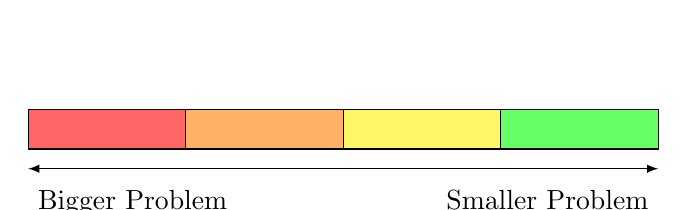
\begin{tikzpicture}
    \draw[draw=white] (-4,1) -- (4,1);
    \draw[draw=black, fill=red!60] (-4,0.5) rectangle (-2,0);
    \draw[draw=black, fill=orange!60] (-2,0.5) rectangle (0,0);
    \draw[draw=black, fill=yellow!60] (0,0.5) rectangle (2,0);
    \draw[draw=black, fill=green!60] (2,0.5) rectangle (4,0);
    \draw[draw=black, latex-latex] (-4,-0.25) -- (4,-0.25);
    \node[black, anchor=north west] at (-4,-0.4) {Bigger Problem};
    \node[black, anchor=north east] at (4,-0.4) {Smaller Problem};
\end{tikzpicture}
\caption{Structure Diagram (\nth{2} prototype)}\label{fig:structDiagram2}
\end{figure}

Figure \ref{fig:structDiagram2} shows this project's structure, breaking down the larger problem of the entire app, into a series of smaller problems which are easier to consider. Some of the problems listed above were present in the first structure diagram, but they have been added to this one as well as I have not yet implemented them. I will go into more detail for each of the smaller problems above (further decomposing them), in the approximate order I would be implementing them.

\section{Authentication System}\label{sec:authenticationSystem}
\subsection{Storing Data \& Encryption}\label{sec:encryption}
In the second prototype, users will be able to create and log into an account, which they can use to save regions they have predicted. I will be using MongoDB to store this data, which allows for \pil{json} objects to be stored in ``collections'' (tables).

Most of the data I will be entering can just be stored as it is, but the user's password must be encrypted, to ensure security. One thing we can do to encrypt the password is to pass it through a hashing function.

Hashing functions (such as \pil{sha256} or \pil{MD5}) take in an input and generate a unique, fixed-length key as an output, obscuring the original meaning. Hashing functions are also impossible to reverse-engineer, meaning that if a hacker gets a hold of hashed passwords, they will not be able to find the original password.

\begin{figure}[H]
\centering
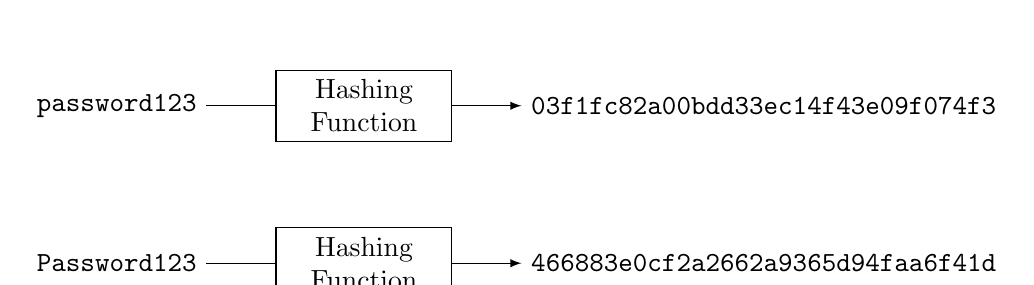
\begin{tikzpicture}
    % example 1
    \node[anchor=east] at (1,0) {\texttt{password123}};
    \draw[-latex] (1,0) -- (5,0);
    \node[anchor=west] at (5,0) {\texttt{03f1fc82a00bdd33ec14f43e09f074f3}};
    \node[draw, text width=2cm, align=center, fill=white] at (3,0) {Hashing Function};
    % example 2
    \node[anchor=east] at (1,-2) {\texttt{Password123}};
    \draw[-latex] (1,-2) -- (5,-2);
    \node[anchor=west] at (5,-2) {\texttt{466883e0cf2a2662a9365d94faa6f41d}};
    \node[draw, text width=2cm, align=center, fill=white] at (3,-2) {Hashing Function};
\end{tikzpicture}
\caption{Hashing Examples}
\end{figure}

As the hashed output is based on the entire input, changing the input only slightly (for example, ``p'' to ``P'') will have a big effect on the output, which makes it harder for hackers to look for patterns.

However, humans are often predictable, and many of them use the same, easy to guess, password (even I have done it in the example). Therefore, if a hacker has a list of common passwords, they can pass them through the hashing function, and compare them against the database. Alternatively, they could use a ``rainbow table'', which is a table of common passwords, along with the hashed versions, which means they don't need to compute any hashes. 

To avoid this, we can add salt to the passwords, before we hash them. This is where we append a random set of characters to the beginning of the password, before hashing. The salt (random characters) will be stored alongside the password, so that we can reconstruct the hashed password.

\begin{figure}[H]
\centering
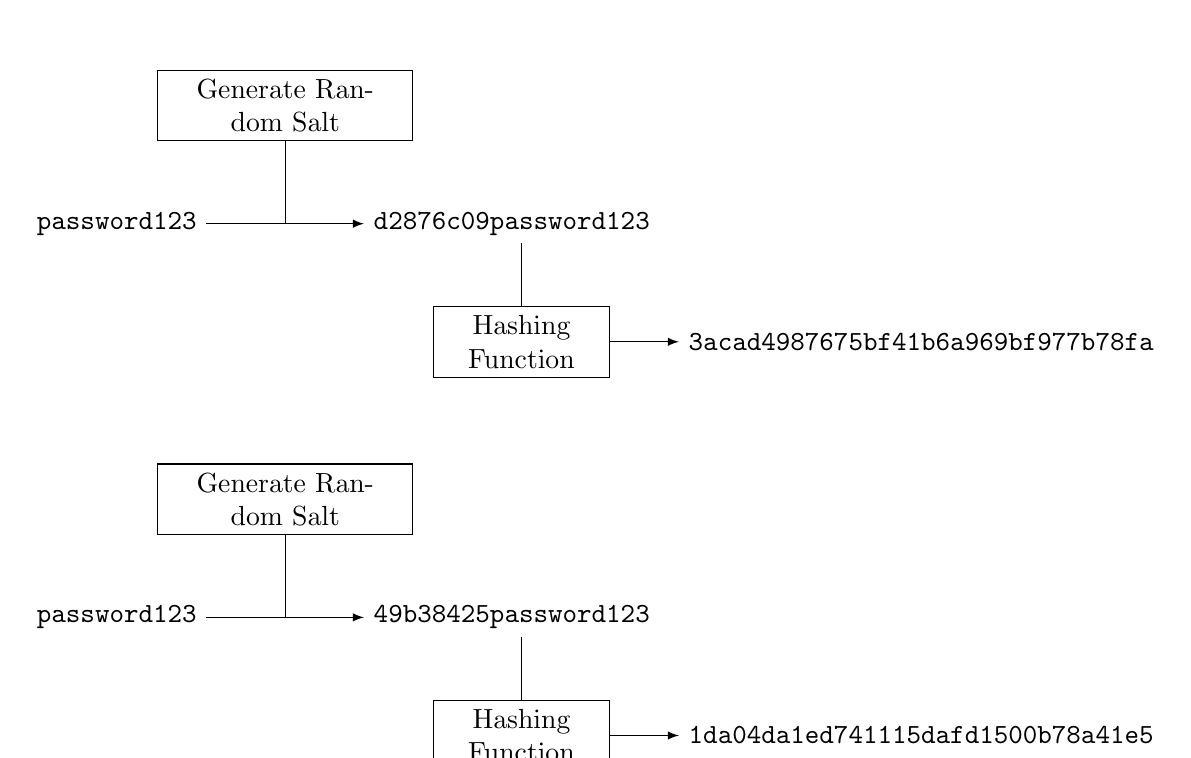
\begin{tikzpicture}
    % example 1
    \node[anchor=east] at (1,0) {\texttt{password123}};
    \draw[] (2,1.5) -- (2,0);
    \draw[-latex] (1,0) -- (3,0);
    \node[anchor=west] at (3,0) {\texttt{d2876c09password123}};
    \draw[] (5,-0.25) -- (5,-1.5);
    \draw[-latex] (5,-1.5) -- (7,-1.5);
    \node[anchor=west] at (7,-1.5) {\texttt{3acad4987675bf41b6a969bf977b78fa}};
    \node[draw, text width=3cm, align=center, fill=white] at (2,1.5) {Generate Random Salt};
    \node[draw, text width=2cm, align=center, fill=white] at (5,-1.5) {Hashing Function};
    % example 2
    \node[anchor=east] at (1,-5) {\texttt{password123}};
    \draw[] (2,-3.5) -- (2,-5);
    \draw[-latex] (1,-5) -- (3,-5);
    \node[anchor=west] at (3,-5) {\texttt{49b38425password123}};
    \draw[] (5,-5.25) -- (5,-6.5);
    \draw[-latex] (5,-6.5) -- (7,-6.5);
    \node[anchor=west] at (7,-6.5) {\texttt{1da04da1ed741115dafd1500b78a41e5}};
    \node[draw, text width=3cm, align=center, fill=white] at (2,-3.5) {Generate Random Salt};
    \node[draw, text width=2cm, align=center, fill=white] at (5,-6.5) {Hashing Function};
\end{tikzpicture}
\caption{Salting Examples}
\end{figure}

In the first example, what would be stored in the database would be \texttt{d2876c09} for the salt and \texttt{3acad4987675bf41b6a969bf977b78fa} for the hashed password.

This protects agains the rainbow tables, as the hackers will then have to add the salt to each of their common passwords, and then run the hashing function, instead of just using a table. However, we should also attempt to protect against doing that, as it is still pretty easy.

One way to do this, is to ensure that we use a slow hashing algorithm. Many high-end GPUs can compute billions of hashes per second, if we don't use a slow hashing algorithm, but can only compute thousands of them if we do. The slow hashing algorithm I will be using is called \pil{bcrypt}.

\subsection{Account Management}\label{sec:accountManagement}
\subsubsection{Creating an Account}
The first thing the user must do when creating an account is select a username, but we must check that the username they select does not already exist. If it doesn't, they can write their password, validating with double entry validation. If they match, the user can submit and the password will be salted and hashed. The username, the hashed password, and the salt will be stored in the MongoDB.

\begin{figure}[H]
\centering
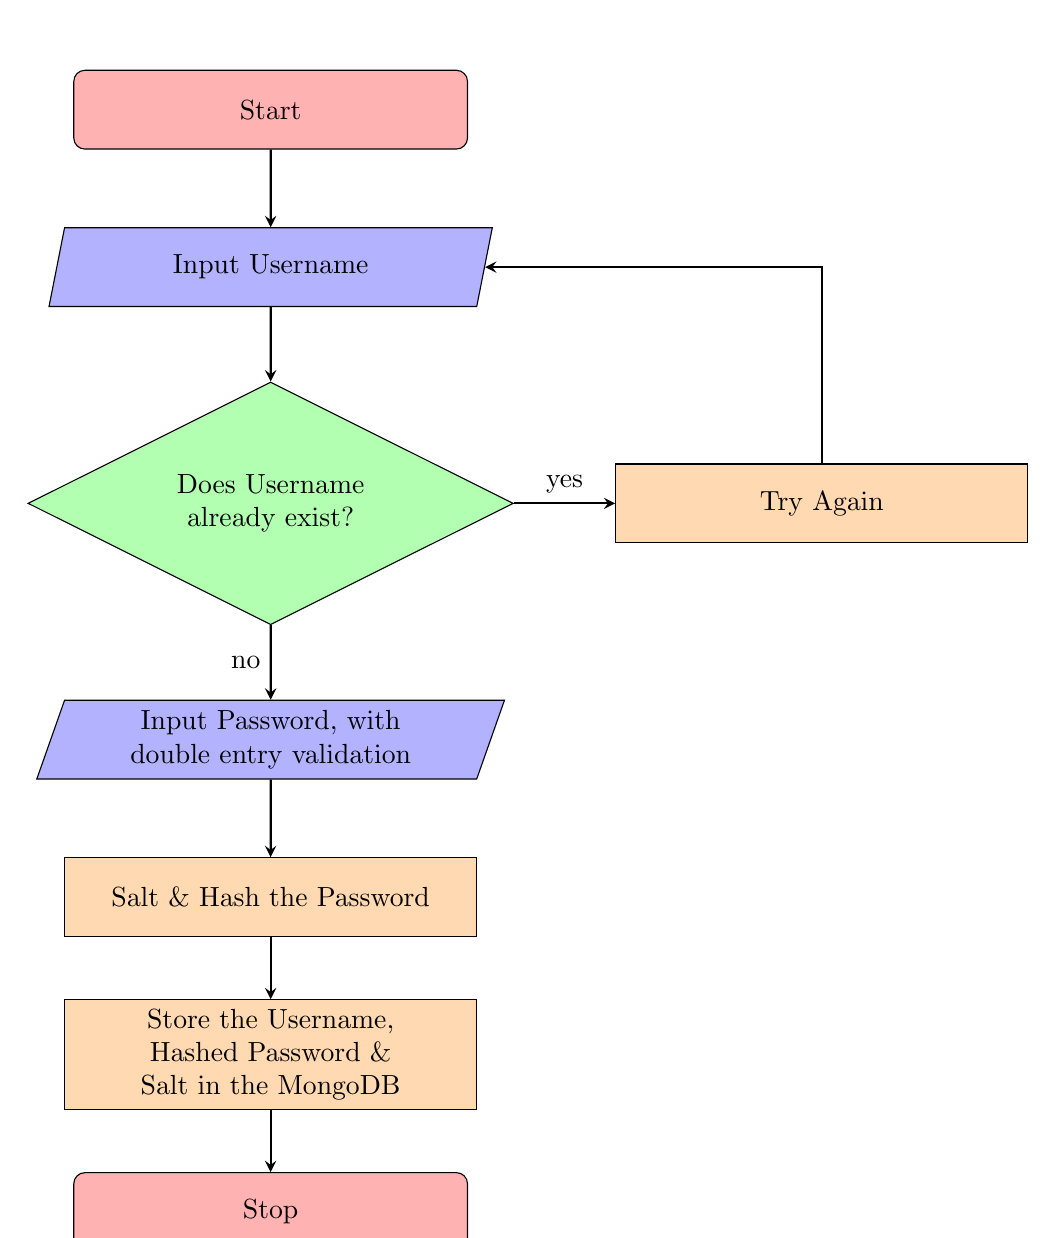
\begin{tikzpicture}[node distance=2cm]
    \node (start) [fStartStop] {Start};
    \node (username) [fInputOutput, below of=start] {Input Username};
    \node (usernameExists) [fDecision, below of=username, yshift=-1cm] {Does Username already exist?};
    \node (tryAgain) [fProcess, right of=usernameExists, xshift=5cm] {Try Again};
    \node (password) [fInputOutput, yshift=-1cm, below of=usernameExists] {Input Password, with double entry validation};
    \node (hashPassword) [fProcess, below of=password] {Salt \& Hash the Password};
    \node (storeDB) [fProcess, below of=hashPassword] {Store the Username, Hashed Password \& Salt in the MongoDB};
    \node (stop) [fStartStop, below of=storeDB] {Stop};
    
    \draw [fArrow] (start) -- (username);
    \draw [fArrow] (username) -- (usernameExists);
    \draw [fArrow] (usernameExists) -- node[anchor=east] {no} (password);
    \draw [fArrow] (usernameExists) -- node[anchor=south] {yes} (tryAgain);
    \draw [fArrow] (tryAgain) |- (username);
    \draw [fArrow] (password) -- (hashPassword);
    \draw [fArrow] (hashPassword) -- (storeDB);
    \draw [fArrow] (storeDB) -- (stop);
\end{tikzpicture}
\caption{Creating an Account Flowchart}
\end{figure}

\subsubsection{Logging in}
When logging in to an existing account, the user will enter their username and password. We must check if the username exists, and if it does, we can retrieve the salt, add it to the password and hash it, and compare that against the hashed password in the database. If it matches, we can grant access, otherwise they can try again.

\begin{figure}[H]
\centering
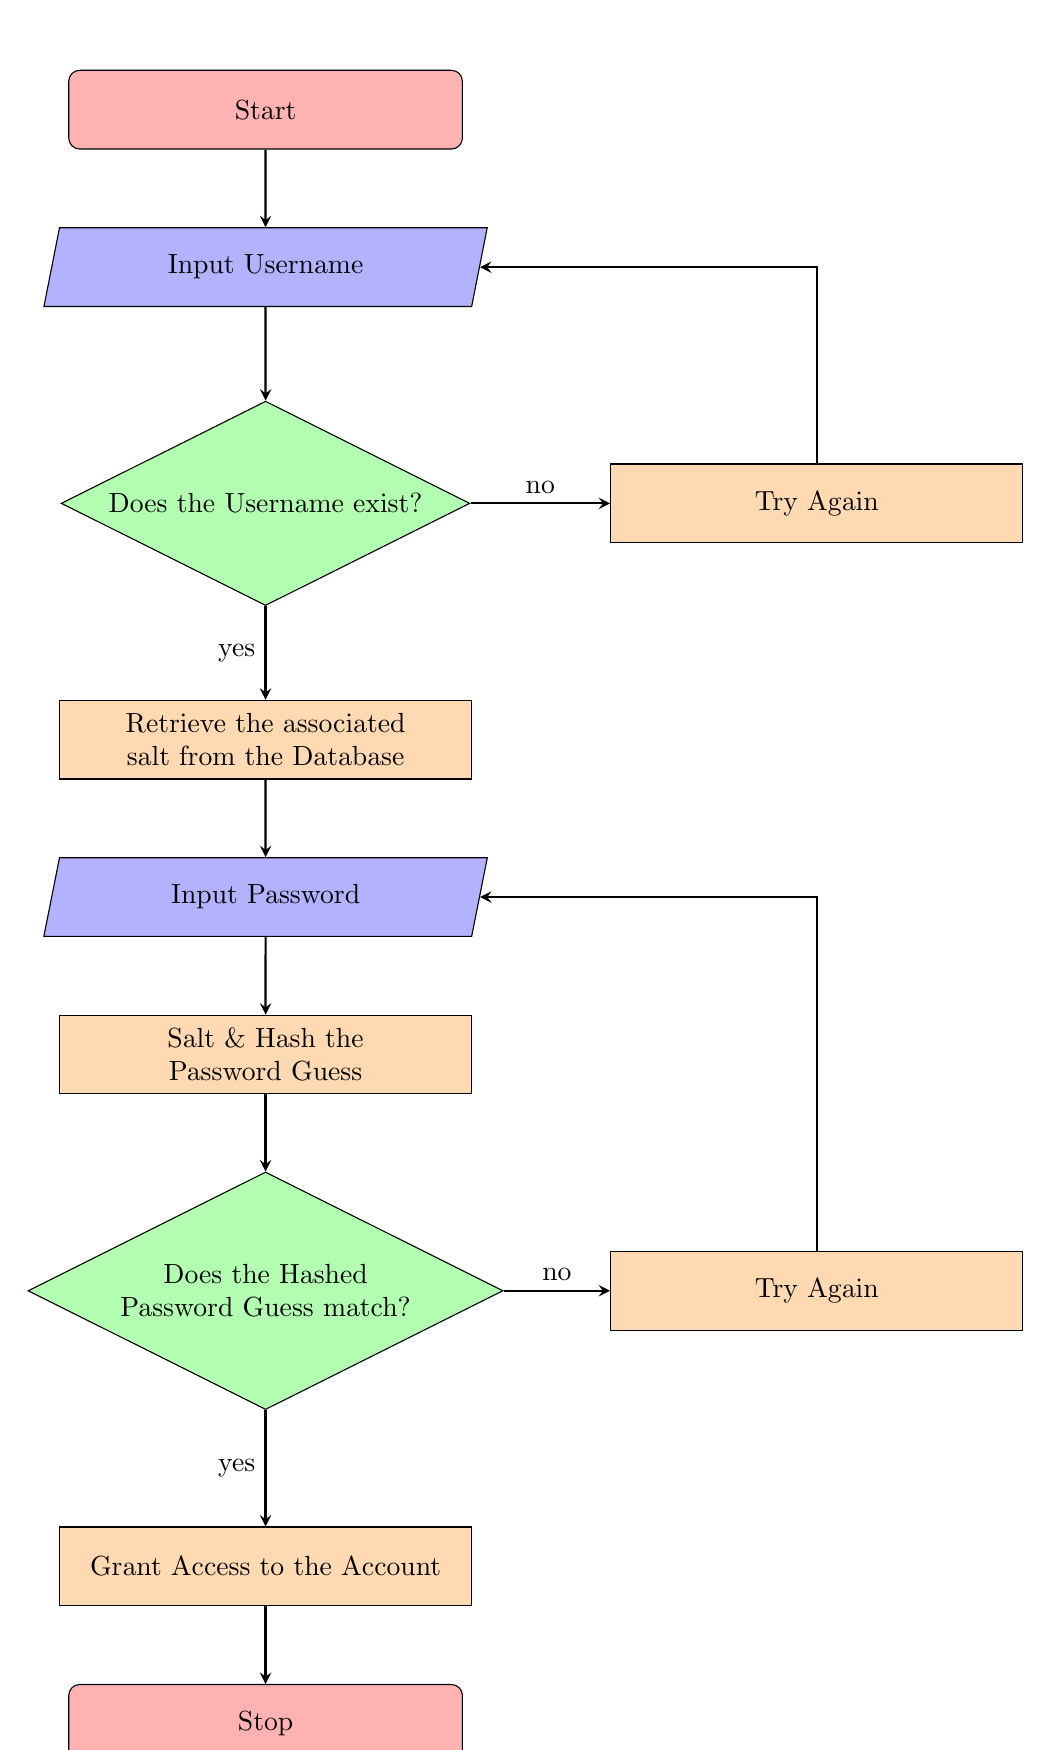
\begin{tikzpicture}[node distance=2cm]
    \node (start) [fStartStop] {Start};
    \node (username) [fInputOutput, below of=start] {Input Username};
    \node (usernameExists) [fDecision, below of=username, yshift=-1cm] {Does the Username exist?};
    \node (tryAgain) [fProcess, right of=usernameExists, xshift=5cm] {Try Again};
    \node (retrieveSalt) [fProcess, yshift=-1cm, below of=usernameExists] {Retrieve the associated salt from the Database};
    \node (password) [fInputOutput, below of=retrieveSalt] {Input Password};
    \node (hashPassword) [fProcess, below of=password] {Salt \& Hash the Password Guess};
    \node (correctGuess) [fDecision, below of=hashPassword, yshift=-1cm] {Does the Hashed Password Guess match?};
    \node (tryAgain2) [fProcess, right of=correctGuess, xshift=5cm] {Try Again};
    \node (grantAccess) [fProcess, below of=correctGuess, yshift=-1.5cm] {Grant Access to the Account};
    \node (stop) [fStartStop, below of=grantAccess] {Stop};
    
    \draw [fArrow] (start) -- (username);
    \draw [fArrow] (username) -- (usernameExists);
    \draw [fArrow] (usernameExists) -- node[anchor=east] {yes} (retrieveSalt);
    \draw [fArrow] (usernameExists) -- node[anchor=south] {no} (tryAgain);
    \draw [fArrow] (tryAgain) |- (username);
    \draw [fArrow] (retrieveSalt) -- (password);
    \draw [fArrow] (password) -- (hashPassword);
    \draw [fArrow] (hashPassword) -- (correctGuess);
    \draw [fArrow] (correctGuess) -- node[anchor=east] {yes} (grantAccess);
    \draw [fArrow] (correctGuess) -- node[anchor=south] {no} (tryAgain2);
    \draw [fArrow] (tryAgain2) |- (password);
    \draw [fArrow] (grantAccess) -- (stop);
\end{tikzpicture}
\caption{Logging In Flowchart}
\end{figure}

\subsection{List of Key Variables}
\subsubsection{Variables in Creating an Account}
\begin{center}
\begin{longtable}{ | m{3cm} | m{4cm}| m{4cm} | m{4cm} |} 
    \hline
    \textbf{Identifier} & \textbf{Data Type} & \textbf{Explanation}  & \textbf{Justification} \\ 
    \hline
    \pil{username} & \pil{str} & Stores what the user entered as their username & Must be checked against the database to see if it exists already \\ 
    \hline
    \pil{password} & \pil{str} & Stores what the user entered as their password & All accounts should have a password for authentication \\ 
    \hline
    \pil{password2} & \pil{str} & Stores what the user enetered as their password, in the second field & This ensures double entry validation \\ 
    \hline
    \pil{salt} & \pil{str} (hex) & Stores the random characters that will be added to the password & The salt must be added to the database with the password \\ 
    \hline
    \pil{hashed_password} & \pil{str} (hex) & Stores the password after it has been salted and hashed & This is what will be stored in the database for us to check against \\ 
    \hline
\caption{List of Key Variables in Creating an Account}
\end{longtable}
\end{center}

\subsubsection{Variables in Logging In}
\begin{center}
\begin{longtable}{ | m{3cm} | m{4cm}| m{4cm} | m{4cm} |} 
    \hline
    \textbf{Identifier} & \textbf{Data Type} & \textbf{Explanation}  & \textbf{Justification} \\ 
    \hline
    \pil{username} & \pil{str} & Stores what the user entered as their username & Must be checked against the database to see if it exists \\ 
    \hline
    \pil{salt} & \pil{str} (hex) & Stores the random characters that were added to the password & Retrieved from the database, to get the same hash \\ 
    \hline
    \pil{password} & \pil{str} & Stores what the user entered as their password & All accounts should have a password for authentication \\ 
    \hline
    \pil{hashed_password} & \pil{str} (hex) & Stores the salted and hashed version of what the user entered as their password & Used to check if what they have entered is correct \\ 
    \hline
    \pil{correct_hashed_password} & \pil{str} (hex) & Stores the correct salted and hashed password & Used to check against the password guess, if they match we can grant access to the account \\ 
    \hline
\caption{List of Key Variables in Logging In}
\end{longtable}
\end{center}

\subsubsection{Other Variables}
\begin{center}
\begin{longtable}{ | m{3cm} | m{4cm}| m{4cm} | m{4cm} |} 
    \hline
    \textbf{Identifier} & \textbf{Data Type} & \textbf{Explanation}  & \textbf{Justification} \\ 
    \hline
    \pil{database} & \pil{object} & Stores the database from MongoDB & We must be able to retrieve values from it, in order to authenticate the user \\ 
    \hline
\caption{List of Other Key Variables in Authentication System}
\end{longtable}
\end{center}

\section{User Interface}\label{sec:ui2}
\subsection{Interface Sketch -- A Tabbed Interface}\label{sec:ui2sketches}
As seen before, when implemeting the GUI, Gradio offers different ways to arrange elements (For example, I have used \pil{gr.Row()}, \pil{gr.Column()} and \pil{gr.Group()}). Another one that we can make use of is \pil{gr.Tab()}, which will place all of its elements inside a tab. Other \pil{gr.Tab()} elements on the same level will appear next to each other, for the user to switch between.  

\begin{figure}[H]
\centering
\begin{tikzpicture}
    % border
    \draw (0,0) rectangle (15,12);
    % tabs
    \draw (0,12) rectangle (2,12.65);
    \draw (1,12.65) node[anchor=north] {Predict};
    \draw (2,12) rectangle (4,12.65);
    \draw (3,12.65) node[black!60,anchor=north] {Compare};
    \draw (4,12) rectangle (6,12.65);
    \draw (5,12.65) node[black!60,anchor=north] {Regions};
    \draw (6,12) rectangle (8,12.65);
    \draw (7,12.65) node[black!60,anchor=north] {Log In};
    \draw (8,12) rectangle (10,12.65);
    \draw (9,12.65) node[black!60,anchor=north] {Sign Up};
    \draw (10,12) rectangle (12,12.65);
    \draw (11,12.65) node[black!60,anchor=north] {Help};
    % map
    \path[fill stretch image=map] (0.5,11.5) rectangle (9,6);
    \draw (0.5,11.5) rectangle (9,6);
    \draw[fill=white] (0.5,11.5) rectangle (1,11);
    \draw (0.65,11.1) -- (0.588196601125,11.290211303259) -- (0.75,11.4077683537175) -- (0.911803398875,11.290211303259) -- (0.85,11.1) -- cycle;
    \draw[fill=white] (0.5,10.75) rectangle (1,10.25);
    \draw (0.6,10.5) -- (0.9,10.5);
    \draw (0.75,10.65) -- (0.75,10.35);
    \draw[fill=white] (0.5,10.25) rectangle (1,9.75);
    \draw (0.6,10) -- (0.9,10);
    \draw[fill=white] (0.5,9.5) rectangle (1,9);
    \draw (0.6,9.4) -- (0.9,9.1);
    \draw (0.6,9.1) -- (0.9,9.4);
    \draw[blue,fill=blue!80,fill opacity=0.4] (1.65,9.25) rectangle (3,8.5);
    \filldraw[red] (2.3,8.9) circle (0.05); 
    %predict button section
    \draw[fill=orange] (9.5,11.5) rectangle (14.5,10.5) node[pos=0.5] {Predict};
    \draw (9.5,10) node[anchor=north west] {{\scriptsize I believe the HDI of this area is...}};
    \draw (9.5,10) rectangle (14.5,8.5) node[pos=0.5] {0.927};
    \draw (9.5,8) node[anchor=north west] {{\scriptsize That's a similar HDI to...}};
    \draw (9.5,8) rectangle (14.5,6) node[pos=0.5] {The USA};
    %suggestions
    \draw (0.5,4.5) node[anchor=south west] {{\scriptsize New Building}};
    \draw (3,4.5) node[anchor=south west] {{\scriptsize Coordinates}};
    \draw (9,4.5) node[anchor=south west] {{\scriptsize New HDI}};
    \draw (11.5,4.5) node[anchor=south west] {{\scriptsize Change in HDI}};
    \draw (0.5,4.5) rectangle (3,4) node[pos=0.5] {School};
    \draw (3,4.5) rectangle (9,4) node[pos=0.5] {$36.922883^{\circ}\text{N},-101.709461^{\circ}\text{E}$};
    \draw (9,4.5) rectangle (11.5,4) node[pos=0.5] {0.928};
    \draw (11.5,4.5) rectangle (14.5,4) node[pos=0.5] {$+0.001$};
    \draw[fill=cyan!20] (0.5,4) rectangle (3,3.5) node[pos=0.5] {Hospital};
    \draw[fill=cyan!20] (3,4) rectangle (9,3.5) node[pos=0.5] {$43.919052^{\circ}\text{N},-106.264212^{\circ}\text{E}$};
    \draw[fill=cyan!20] (9,4) rectangle (11.5,3.5) node[pos=0.5] {0.929};
    \draw[fill=cyan!20] (11.5,4) rectangle (14.5,3.5) node[pos=0.5] {$+0.002$};
    \draw (0.5,3.5) rectangle (3,3) node[pos=0.5] {Library};
    \draw (3,3.5) rectangle (9,3) node[pos=0.5] {$36.954162^{\circ}\text{N},-87.008695^{\circ}\text{E}$};
    \draw (9,3.5) rectangle (11.5,3) node[pos=0.5] {0.928};
    \draw (11.5,3.5) rectangle (14.5,3) node[pos=0.5] {$+0.001$};
    \draw (7.5,2.5) node {$\vdots$};
    % note
    \draw (0,0) node[anchor=south west] {{\scriptsize (The data presented in this sketch is completely made up but somewhat realistic)}};
    % annotations
    \draw[red,->] (1,13.65) node[red,above] {1.} -- (1,12.65);
    \draw[red,->] (7,13.65) node[red,above] {2.} -- (7,13);
\end{tikzpicture}
\caption{Technical Interface Sketch (\nth{2} prototype, main page)}\label{fig:interfaceSketch2.1}
\end{figure}

Figure \ref{fig:interfaceSketch2.1} shows the main prediction page for the app, which I have already implemented, and so most of these elements are not labelled. The elements that are labelled are:

\begin{enumerate}
    \item Currently Selected Tab
    \item Other Tabs
\end{enumerate}
The contents of the other 5 tabs are illustrated below, in Figures \ref{fig:interfaceSketch2.2} to \ref{fig:interfaceSketch2.6}.

\begin{figure}[H]
\centering
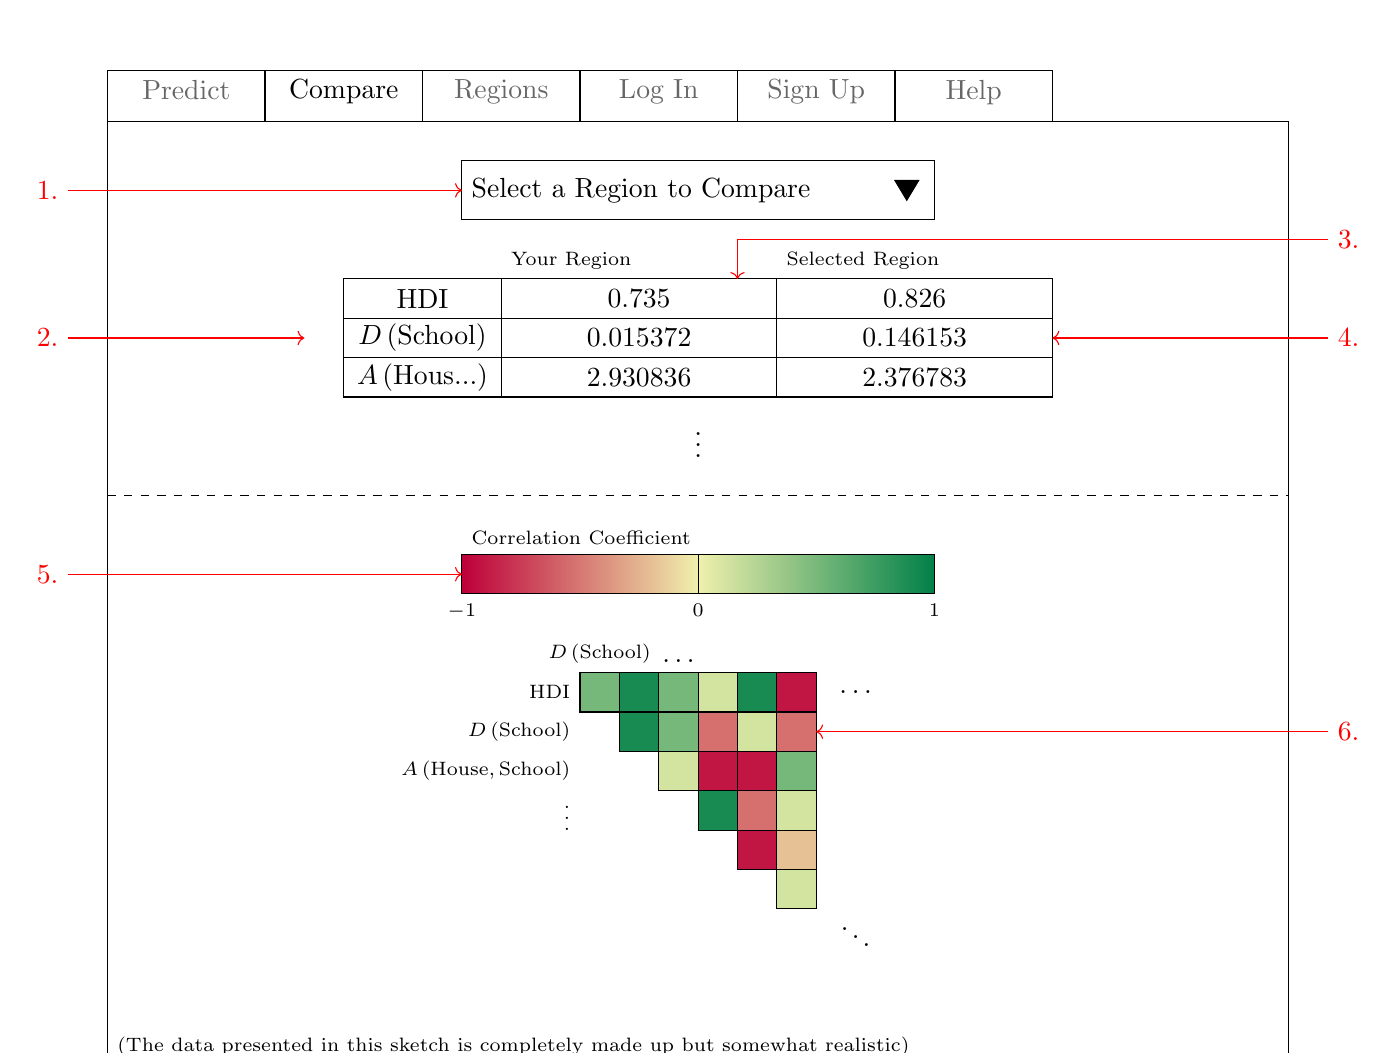
\begin{tikzpicture}
    % border
    \draw (0,0) rectangle (15,12);
    % tabs
    \draw (0,12) rectangle (2,12.65);
    \draw (1,12.65) node[black!60,anchor=north] {Predict};
    \draw (2,12) rectangle (4,12.65);
    \draw (3,12.65) node[anchor=north] {Compare};
    \draw (4,12) rectangle (6,12.65);
    \draw (5,12.65) node[black!60,anchor=north] {Regions};
    \draw (6,12) rectangle (8,12.65);
    \draw (7,12.65) node[black!60,anchor=north] {Log In};
    \draw (8,12) rectangle (10,12.65);
    \draw (9,12.65) node[black!60,anchor=north] {Sign Up};
    \draw (10,12) rectangle (12,12.65);
    \draw (11,12.65) node[black!60,anchor=north] {Help};
    % dropdown
    \draw (4.5,11.5) rectangle (10.5,10.75);
    \draw (4.5,11.125) node[anchor=west] {Select a Region to Compare};
    \draw[black,fill=black] (10,11.25) -- (10.3,11.25) -- (10.15,11) -- cycle;
    % comparing to selected region
    \draw (5,10) node[anchor=south west] {{\scriptsize Your Region}};
    \draw (8.5,10) node[anchor=south west] {{\scriptsize Selected Region}};
    \draw (3,10) rectangle (5,9.5) node[pos=0.5] {HDI};
    \draw (5,10) rectangle (8.5,9.5) node[pos=0.5] {0.735};
    \draw (8.5,10) rectangle (12,9.5) node[pos=0.5] {0.826};
    \draw (3,9.5) rectangle (5,9) node[pos=0.5] {$D\left(\text{School}\right)$};
    \draw (5,9.5) rectangle (8.5,9) node[pos=0.5] {0.015372};
    \draw (8.5,9.5) rectangle (12,9) node[pos=0.5] {0.146153};
    \draw (3,9) rectangle (5,8.5) node[pos=0.5] {$A\left(\text{Hous...}\right)$};
    \draw (5,9) rectangle (8.5,8.5) node[pos=0.5] {2.930836};
    \draw (8.5,9) rectangle (12,8.5) node[pos=0.5] {2.376783};
    \draw (7.5,8) node {$\vdots$};
    % separator
    \draw[dashed] (0,7.25) -- (15,7.25);
    % gradient key
    \definecolor{gradient1}{RGB}{189, 0, 57}
    \definecolor{gradient2}{RGB}{240, 240, 173}
    \definecolor{gradient3}{RGB}{0, 128, 72}
    \draw[shading=axis, left color=gradient1, right color=gradient2] (4.5,6.5) rectangle (7.5,6);
    \draw[shading=axis, left color=gradient2, right color=gradient3] (7.5,6.5) rectangle (10.5,6);
    \draw (4.5,6.5) node[anchor=south west] {{\scriptsize Correlation Coefficient}};
    \draw (4.5,6) node[anchor=north] {{\scriptsize $-1$}};
    \draw (7.5,6) node[anchor=north] {{\scriptsize $0$}};
    \draw (10.5,6) node[anchor=north] {{\scriptsize $1$}};
    % heatmap
    \definecolor{heatmap1}{RGB}{193,21,67}
    \definecolor{heatmap2}{RGB}{213,112,111}
    \definecolor{heatmap3}{RGB}{230,193,150}
    \definecolor{heatmap4}{RGB}{211,227,160}
    \definecolor{heatmap5}{RGB}{118,183,122}
    \definecolor{heatmap6}{RGB}{24,139,82}
    \draw[fill=heatmap5] (6,5) rectangle (6.5,4.5);
    \draw[fill=heatmap6] (6.5,5) rectangle (7,4.5);
    \draw[fill=heatmap5] (7,5) rectangle (7.5,4.5);
    \draw[fill=heatmap4] (7.5,5) rectangle (8,4.5);
    \draw[fill=heatmap6] (8,5) rectangle (8.5,4.5);
    \draw[fill=heatmap1] (8.5,5) rectangle (9,4.5);
    \draw[fill=heatmap6] (6.5,4.5) rectangle (7,4);
    \draw[fill=heatmap5] (7,4.5) rectangle (7.5,4);
    \draw[fill=heatmap2] (7.5,4.5) rectangle (8,4);
    \draw[fill=heatmap4] (8,4.5) rectangle (8.5,4);
    \draw[fill=heatmap2] (8.5,4.5) rectangle (9,4);
    \draw[fill=heatmap4] (7,4) rectangle (7.5,3.5);
    \draw[fill=heatmap1] (7.5,4) rectangle (8,3.5);
    \draw[fill=heatmap1] (8,4) rectangle (8.5,3.5);
    \draw[fill=heatmap5] (8.5,4) rectangle (9,3.5);
    \draw[fill=heatmap6] (7.5,3.5) rectangle (8,3);
    \draw[fill=heatmap2] (8,3.5) rectangle (8.5,3);
    \draw[fill=heatmap4] (8.5,3.5) rectangle (9,3);
    \draw[fill=heatmap1] (8,3) rectangle (8.5,2.5);
    \draw[fill=heatmap3] (8.5,3) rectangle (9,2.5);
    \draw[fill=heatmap4] (8.5,2.5) rectangle (9,2);
    \draw (9.5,4.75) node {$\hdots$};
    \draw (9.5,1.75) node {$\ddots$};
    \draw (6,4.75) node[anchor=east] {{\scriptsize HDI}};
    \draw (6,4.25) node[anchor=east] {{\scriptsize $D\left(\text{School}\right)$}};
    \draw (6,3.75) node[anchor=east] {{\scriptsize $A\left(\text{House},\text{School}\right)$}};
    \draw (6,3.25) node[anchor=east] {{\scriptsize $\vdots$}};
    \draw (6.25,5) node[anchor=south] {{\scriptsize $D\left(\text{School}\right)$}};
    \draw (7.25,5) node[anchor=south] {$\hdots$};
    % note
    \draw (0,0) node[anchor=south west] {{\scriptsize (The data presented in this sketch is completely made up but somewhat realistic)}};
    % annotations
    \draw[red,->] (-0.5,11.125) node[red,left] {1.} -- (4.5,11.125);
    \draw[red,->] (-0.5,9.25) node[red,left] {2.} -- (2.5,9.25);
    \draw[red,->] (15.5,10.5) node[red,right] {3.} -| (8,10);
    \draw[red,->] (15.5,9.25) node[red,right] {4.} -- (12,9.25);
    \draw[red,->] (-0.5,6.25) node[red,left] {5.} -- (4.5,6.25);
    \draw[red,->] (15.5,4.25) node[red,right] {6.} -- (9,4.25);
\end{tikzpicture}
\caption{Technical Interface Sketch (\nth{2} prototype, compare page)}\label{fig:interfaceSketch2.2}
\end{figure}

The labelled items shown on Figure \ref{fig:interfaceSketch2.2} are:

\begin{enumerate}
    \item Dropdown menu to Select a Region to Compare
    \item Table showing the HDI and each of the factors for your region and the chosen region
    \item Column for your region
    \item Column for the chosen region
    \item Key for the correlation between factors and HDI
    \item Correlation Heatmap (Analysis of how much each factor affects the others)
\end{enumerate}

I will go into more detail about the meaning of the key \& heatmap in Section \ref{sec:analysisOfFactors}.

\begin{figure}[H]
\centering
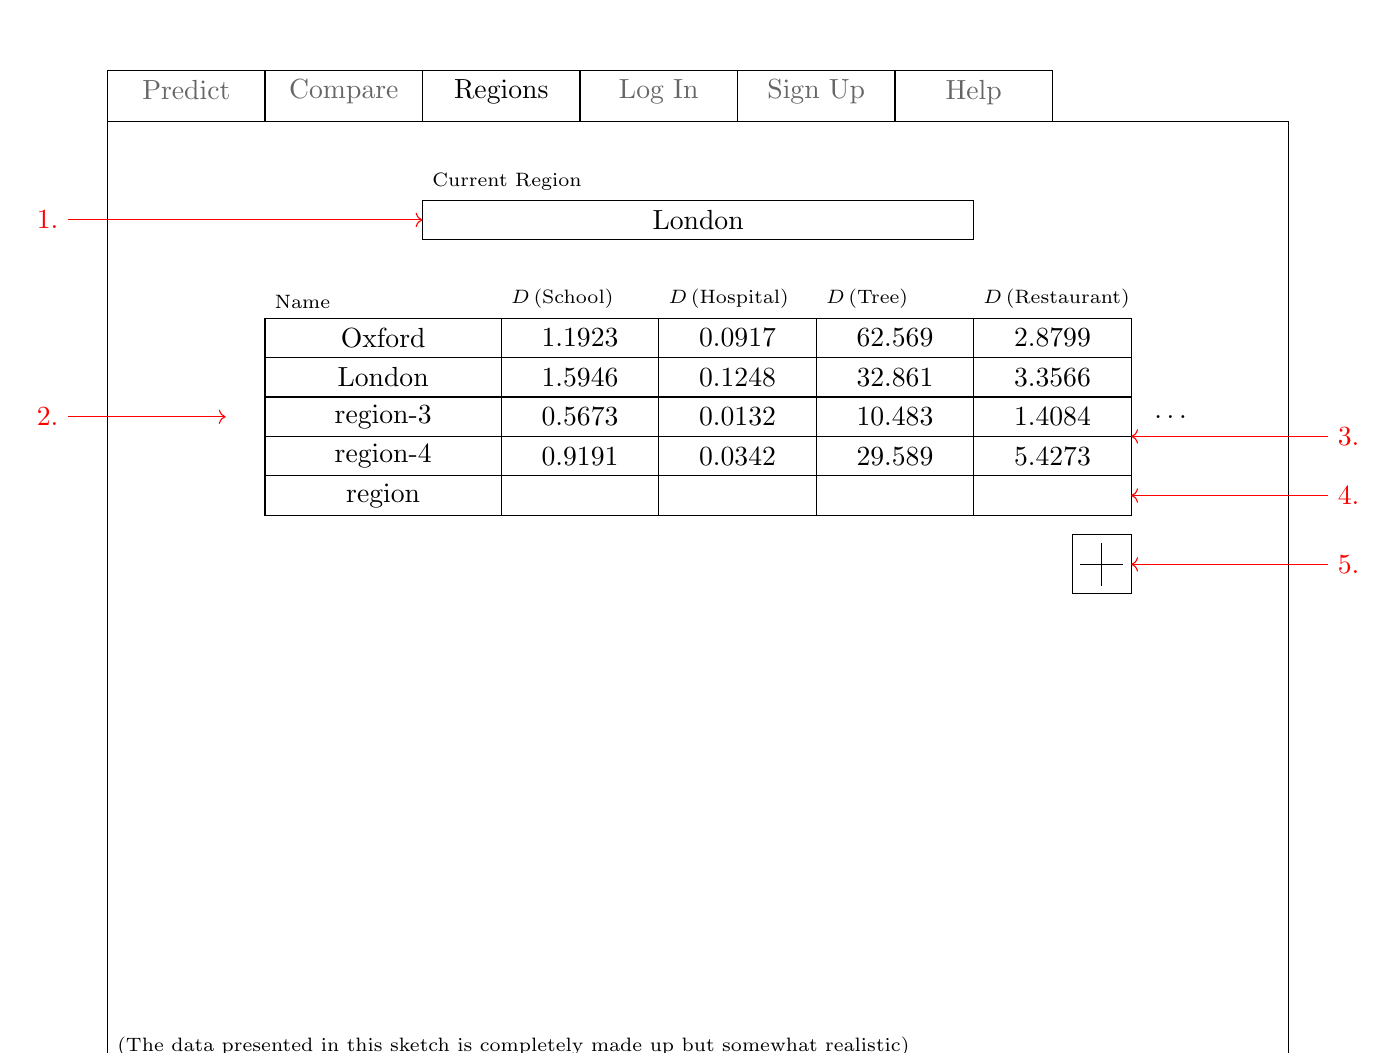
\begin{tikzpicture}
    % border
    \draw (0,0) rectangle (15,12);
    % tabs
    \draw (0,12) rectangle (2,12.65);
    \draw (1,12.65) node[black!60,anchor=north] {Predict};
    \draw (2,12) rectangle (4,12.65);
    \draw (3,12.65) node[black!60,anchor=north] {Compare};
    \draw (4,12) rectangle (6,12.65);
    \draw (5,12.65) node[anchor=north] {Regions};
    \draw (6,12) rectangle (8,12.65);
    \draw (7,12.65) node[black!60,anchor=north] {Log In};
    \draw (8,12) rectangle (10,12.65);
    \draw (9,12.65) node[black!60,anchor=north] {Sign Up};
    \draw (10,12) rectangle (12,12.65);
    \draw (11,12.65) node[black!60,anchor=north] {Help};
    % current region box
    \draw (4,11) node[anchor=south west] {{\scriptsize Current Region}};
    \draw (4,11) rectangle (11,10.5) node[pos=0.5] {London};
    % table
    \draw (2,9.5) node[anchor=south west] {{\scriptsize Name}};
    \draw (5,9.5) node[anchor=south west] {{\scriptsize $D\left(\text{School}\right)$}};
    \draw (7,9.5) node[anchor=south west] {{\scriptsize $D\left(\text{Hospital}\right)$}};
    \draw (9,9.5) node[anchor=south west] {{\scriptsize $D\left(\text{Tree}\right)$}};
    \draw (11,9.5) node[anchor=south west] {{\scriptsize $D\left(\text{Restaurant}\right)$}};
    \draw (2,9.5) rectangle (5,9) node[pos=0.5] {Oxford};
    \draw (5,9.5) rectangle (7,9) node[pos=0.5] {1.1923};
    \draw (7,9.5) rectangle (9,9) node[pos=0.5] {0.0917};
    \draw (9,9.5) rectangle (11,9) node[pos=0.5] {62.569};
    \draw (11,9.5) rectangle (13,9) node[pos=0.5] {2.8799};
    \draw (2,9) rectangle (5,8.5) node[pos=0.5] {London};
    \draw (5,9) rectangle (7,8.5) node[pos=0.5] {1.5946};
    \draw (7,9) rectangle (9,8.5) node[pos=0.5] {0.1248};
    \draw (9,9) rectangle (11,8.5) node[pos=0.5] {32.861};
    \draw (11,9) rectangle (13,8.5) node[pos=0.5] {3.3566};
    \draw (2,8.5) rectangle (5,8) node[pos=0.5] {region-3};
    \draw (5,8.5) rectangle (7,8) node[pos=0.5] {0.5673};
    \draw (7,8.5) rectangle (9,8) node[pos=0.5] {0.0132};
    \draw (9,8.5) rectangle (11,8) node[pos=0.5] {10.483};
    \draw (11,8.5) rectangle (13,8) node[pos=0.5] {1.4084};
    \draw (2,8) rectangle (5,7.5) node[pos=0.5] {region-4};
    \draw (5,8) rectangle (7,7.5) node[pos=0.5] {0.9191};
    \draw (7,8) rectangle (9,7.5) node[pos=0.5] {0.0342};
    \draw (9,8) rectangle (11,7.5) node[pos=0.5] {29.589};
    \draw (11,8) rectangle (13,7.5) node[pos=0.5] {5.4273};
    \draw (2,7.5) rectangle (5,7) node[pos=0.5] {region};
    \draw (5,7.5) rectangle (7,7);
    \draw (7,7.5) rectangle (9,7);
    \draw (9,7.5) rectangle (11,7);
    \draw (11,7.5) rectangle (13,7);
    \draw (13.5,8.25) node {$\hdots$};
    % button
    \draw (12.25,6.75) rectangle (13,6);
    \draw (12.625,6.65) -- (12.625,6.1);
    \draw (12.35,6.375) -- (12.9, 6.375);
    % note
    \draw (0,0) node[anchor=south west] {{\scriptsize (The data presented in this sketch is completely made up but somewhat realistic)}};
    % annotations
    \draw[red,->] (-0.5,10.75) node[red,left] {1.} -- (4,10.75);
    \draw[red,->] (-0.5,8.25) node[red,left] {2.} -- (1.5,8.25);
    \draw[red,->] (15.5,8) node[red,right] {3.} -- (13,8);
    \draw[red,->] (15.5,7.25) node[red,right] {4.} -- (13,7.25);
    \draw[red,->] (15.5,6.375) node[red,right] {5.} -- (13,6.375);
\end{tikzpicture}
\caption{Technical Interface Sketch (\nth{2} prototype, regions page)}\label{fig:interfaceSketch2.3}
\end{figure}

The labelled items shown on Figure \ref{fig:interfaceSketch2.3} are:

\begin{enumerate}
    \item A Textbox showing the region the user has currently selected (it may not always be obvious)
    \item Table for each of the user's regions. The user can choose the name of each one, by typing it into the ``Name'' column.
    \item Examples of regions where the user has not chosen a name
    \item Example of a region where the user has not yet entered the factors
    \item Button to add a row to the table, so that the user can manually enter factors
\end{enumerate}

In this page, the user will be able to switch between the different regions they have processed before. If they are logged in with an account, regions they have processed in a previous session will also appear here. Users can also use this to manually enter factors, by adding rows to this table.

\begin{figure}[H]
\centering
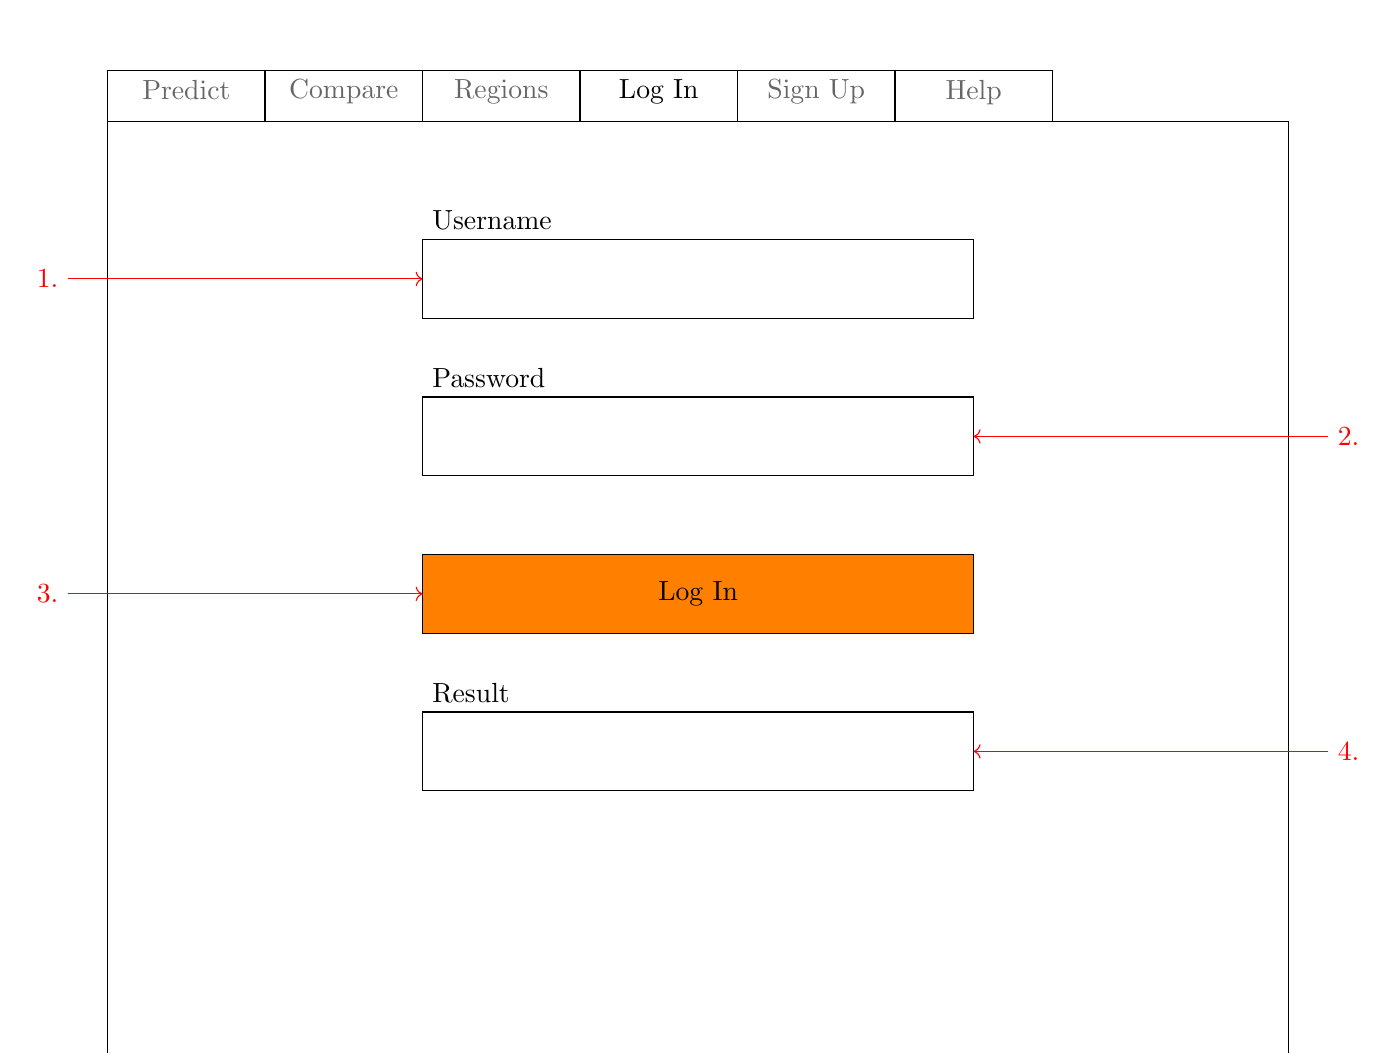
\begin{tikzpicture}
    % border
    \draw (0,0) rectangle (15,12);
    % tabs
    \draw (0,12) rectangle (2,12.65);
    \draw (1,12.65) node[black!60,anchor=north] {Predict};
    \draw (2,12) rectangle (4,12.65);
    \draw (3,12.65) node[black!60,anchor=north] {Compare};
    \draw (4,12) rectangle (6,12.65);
    \draw (5,12.65) node[black!60,anchor=north] {Regions};
    \draw (6,12) rectangle (8,12.65);
    \draw (7,12.65) node[anchor=north] {Log In};
    \draw (8,12) rectangle (10,12.65);
    \draw (9,12.65) node[black!60,anchor=north] {Sign Up};
    \draw (10,12) rectangle (12,12.65);
    \draw (11,12.65) node[black!60,anchor=north] {Help};
    % elements
    \draw (4,10.5) node[anchor=south west] {Username};
    \draw (4,10.5) rectangle (11,9.5);
    \draw (4,8.5) node[anchor=south west] {Password};
    \draw (4,8.5) rectangle (11,7.5);
    \draw[fill=orange] (4,6.5) rectangle (11,5.5) node[pos=0.5] {Log In};
    \draw (4,4.5) node[anchor=south west] {Result};
    \draw (4,4.5) rectangle (11,3.5);
    % annotations
    \draw[red,->] (-0.5,10) node[red,left] {1.} -- (4,10);
    \draw[red,->] (15.5,8) node[red,right] {2.} -- (11,8);
    \draw[red,->] (-0.5,6) node[red,left] {3.} -- (4,6);
    \draw[red,->] (15.5,4) node[red,right] {4.} -- (11,4);
\end{tikzpicture}
\caption{Technical Interface Sketch (\nth{2} prototype, log in page)}\label{fig:interfaceSketch2.4}
\end{figure}

The labelled items shown on Figure \ref{fig:interfaceSketch2.4} are:

\begin{enumerate}
    \item Field for the user to enter their username
    \item Field for the user to enter their password
    \item Log in Button
    \item Output Button showing the result of pressing the button (e.g. Login Success, Username does not exist, or Incorrect Password)
\end{enumerate}

\begin{figure}[H]
\centering
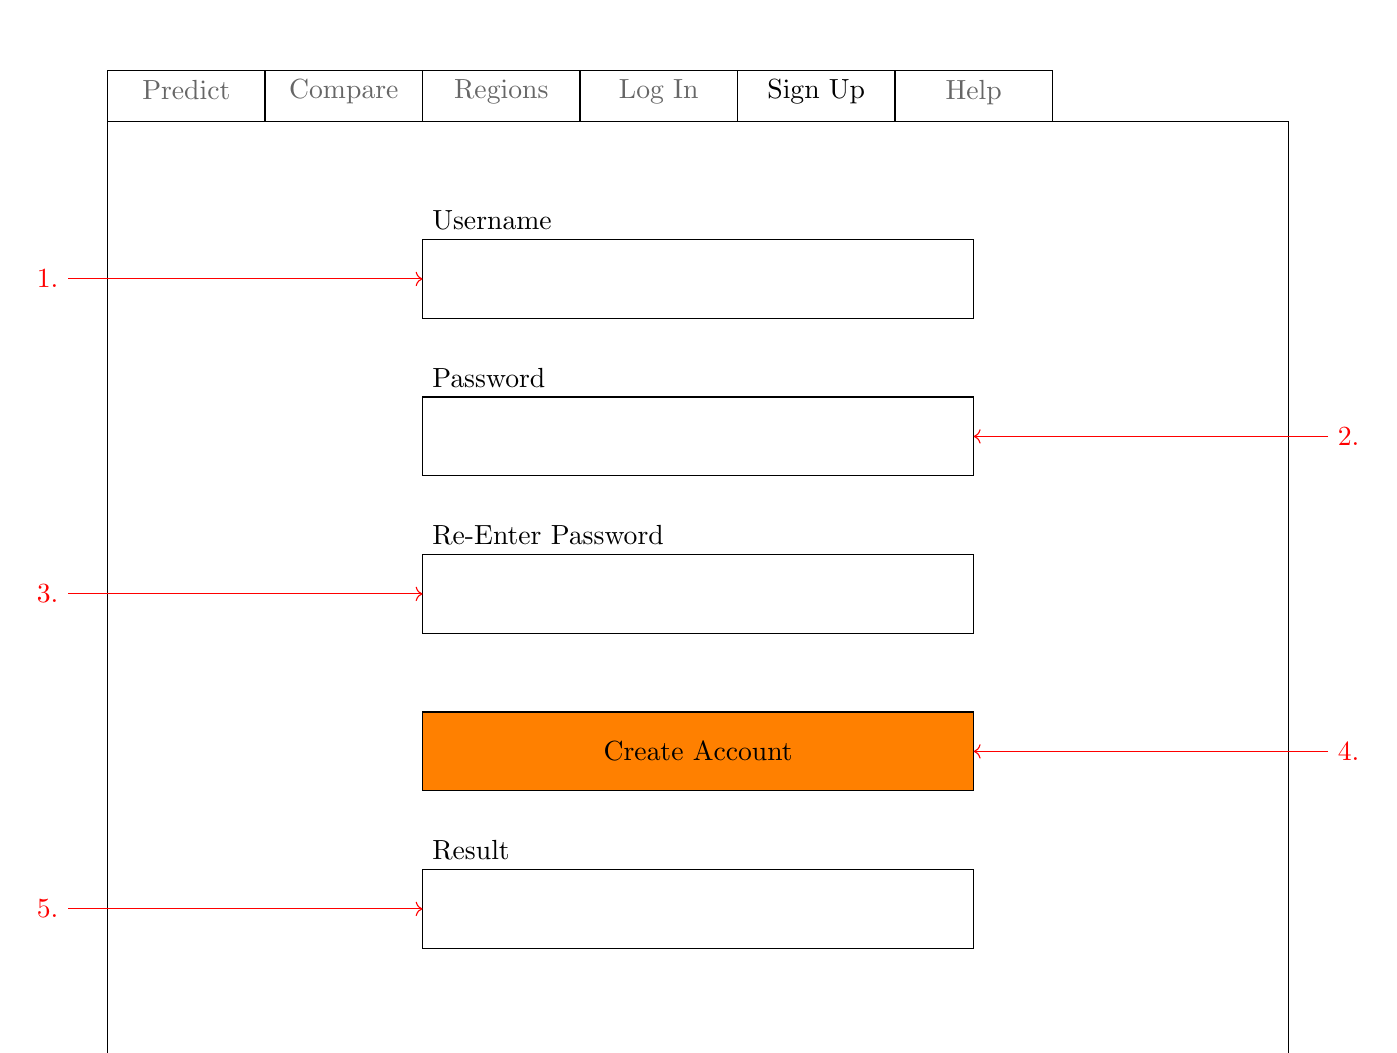
\begin{tikzpicture}
    % border
    \draw (0,0) rectangle (15,12);
    % tabs
    \draw (0,12) rectangle (2,12.65);
    \draw (1,12.65) node[black!60,anchor=north] {Predict};
    \draw (2,12) rectangle (4,12.65);
    \draw (3,12.65) node[black!60,anchor=north] {Compare};
    \draw (4,12) rectangle (6,12.65);
    \draw (5,12.65) node[black!60,anchor=north] {Regions};
    \draw (6,12) rectangle (8,12.65);
    \draw (7,12.65) node[black!60,anchor=north] {Log In};
    \draw (8,12) rectangle (10,12.65);
    \draw (9,12.65) node[anchor=north] {Sign Up};
    \draw (10,12) rectangle (12,12.65);
    \draw (11,12.65) node[black!60,anchor=north] {Help};
    % elements
    \draw (4,10.5) node[anchor=south west] {Username};
    \draw (4,10.5) rectangle (11,9.5);
    \draw (4,8.5) node[anchor=south west] {Password};
    \draw (4,8.5) rectangle (11,7.5);
    \draw (4,6.5) node[anchor=south west] {Re-Enter Password};
    \draw (4,6.5) rectangle (11,5.5);
    \draw[fill=orange] (4,4.5) rectangle (11,3.5) node[pos=0.5] {Create Account};
    \draw (4,2.5) node[anchor=south west] {Result};
    \draw (4,2.5) rectangle (11,1.5);
    % annotations
    \draw[red,->] (-0.5,10) node[red,left] {1.} -- (4,10);
    \draw[red,->] (15.5,8) node[red,right] {2.} -- (11,8);
    \draw[red,->] (-0.5,6) node[red,left] {3.} -- (4,6);
    \draw[red,->] (15.5,4) node[red,right] {4.} -- (11,4);
    \draw[red,->] (-0.5,2) node[red,left] {5.} -- (4,2);
\end{tikzpicture}
\caption{Technical Interface Sketch (\nth{2} prototype, sign up page)}\label{fig:interfaceSketch2.5}
\end{figure}

The labelled items shown on Figure \ref{fig:interfaceSketch2.5} are:

\begin{enumerate}
    \item Field for the user to enter their username
    \item Field for the user to enter their password
    \item Field for the user to re-enter their password (for double-entry validation)
    \item Sign up Button
    \item Output Button showing the result of pressing the button (e.g. Sign Up Success, Username already exists, or Password not Strong Enough, Passwords Do Not Match)
\end{enumerate}

\begin{figure}[H]
\centering
\begin{tikzpicture}
    % border
    \draw (0,0) rectangle (15,12);
    % tabs
    \draw (0,12) rectangle (2,12.65);
    \draw (1,12.65) node[black!60,anchor=north] {Predict};
    \draw (2,12) rectangle (4,12.65);
    \draw (3,12.65) node[black!60,anchor=north] {Compare};
    \draw (4,12) rectangle (6,12.65);
    \draw (5,12.65) node[black!60,anchor=north] {Regions};
    \draw (6,12) rectangle (8,12.65);
    \draw (7,12.65) node[black!60,anchor=north] {Log In};
    \draw (8,12) rectangle (10,12.65);
    \draw (9,12.65) node[black!60,anchor=north] {Sign Up};
    \draw (10,12) rectangle (12,12.65);
    \draw (11,12.65) node[anchor=north] {Help};
    % help
    \draw (2,10.5) -- (8,10.5);
    \draw (3,9.5) -- (14,9.5);
    \draw (3,9) -- (14,9);
    \draw (3,8.5) -- (10,8.5);
    \draw (4,8) -- (14,8);
    \draw (4,7.5) -- (12,7.5);
    \draw (3,7) -- (14,7);
    \draw (3,6.5) -- (7,6.5);
    \draw (4,6) rectangle (12,3);
    \draw (3,2.5) -- (14,2.5);
    \draw (3,2) -- (14,2);
    \draw (3,1.5) -- (8,1.5);
    % annotations
    \draw[red,->] (-0.5,8) node[red,left] {1.} -- (2.5,8);
    \draw[red,->] (15.5,4.5) node[red,right] {2.} -- (12,4.5);
\end{tikzpicture}
\caption{Technical Interface Sketch (\nth{2} prototype, help page)}\label{fig:interfaceSketch2.6}
\end{figure}

The labelled items shown on Figure \ref{fig:interfaceSketch2.6} are:

\begin{enumerate}
    \item Text describing the features of the app (Actual help text not included in this sketch, as I will be writing it as part of the development)
    \item An Image or Diagram to help the understanding
\end{enumerate}

This tab will be written in markdown (which gradio supports), as it allows for basic text formatting, such as different levels of headings, bullet points, ordered lists and tables.

\subsection{Input Validation}
\subsubsection{Authentication System}
When the user creates an account, they will first be prompted to enter a username, which must be a string. Gradio textboxes can only hold strings, so no matter what the user inputs, it will be validated. They must then enter a password, and then re-enter their password, for double entry validation. This is where the user enters data twice, to ensure they have entered the correct data (if the 2 copies do not match, they may have not entered the correct data). In order to ensure that the user uses a secure password, I will be enforcing that the password must be at least 8 characters, using a length check, and that it contains at least 1 number and 1 special character, using a format check. I will also be using a presence check to see if all 3 fields have been filled, otherwise they cannot create an account.

When the user logs into an account, they will again be prompted to enter a username and password. The only input validation that must be done here is a presence check, to ensure they have entered both a username and password.

\subsubsection{Manually Entering Regions}
On the Regions tab (Figure \ref{fig:interfaceSketch2.3}), I will be using a gradio Dataframe for the regions table (which is the same thing we used for the suggestions table), except this time it will be interactive. This means that the user will be able to enter data into any of the cells, as well as create new rows.

To ensure that the data in each column is of the right type (\pil{str} for the Name column, and \pil{float} for everything else), we can specify the datatype of each column. When the user creates a new region by drawing on the map, the name of it will be the same as the filename they uploaded. When the user creates a new region by adding a new row to the dataframe, it will be called ``region''.

\subsubsection{Comparing Regions}
When comparing regions, the only thing the user has to input is which region they wish to compare to. It should only be one of the $\sim 2000$ regions processed in Milestone 1 (Section \ref{sec:milestone1}), and not anything else. I will therefore be using a dropdown menu, instead of something like a textbox. The gradio dropdown menu however can act like a textbox, where the user types to filter the options.

\subsection{Usabilty Features}
\subsubsection{Comparison Page}
On the comparison page, users will be able to choose a region from the training data to compare their region to. They will be presented with a dropdown menu, which will be the top element in the screen (to draw their attention to it), to choose an element from. On the right side of the dropdown menu, there will be a small triangle pointing down, to suggest that clicking on this element will show a dropdown menu. A cursor will also appear when the element is selected, which suggests that they can type to search for a particular region.

The rest of the elements on this page (the table, the correlation coefficient key and the correlation heatmap) will be not be interactive, as all they do is convey information (as opposed to take in information from the user). Everything will be labelled accordingly, and if the user does not understand something (for example, the correlation heatmap), they can go to the help page.

In short, a correlation coefficient of $1$ means the 2 variables have a very strong positive correlation, a correlation coefficient of $-1$ means the 2 variables have a very strong negative correlation, and a correlation coefficient of $0$ means they have no correlaiton. I have therefore chosen the colour to represent 1 to be green and the colour to represent -1 to be deep red, as green often symbolises good and red bad. In the middle, for 0, there is a neutral off-white yellow, to make the gradient from red to green smoother.

\subsubsection{Regions Page}
On the regions page, users will be able to switch between different regions they have previously processed, by selecting rows in the table. They will also be able to add new regions without drawing on the map by adding new rows to the table. It may not be obvious which of their regions is the one they have currently selected, so there will be a textbox at the top of the screen showing which one they have chosen.

Users will know they can add new regions by the fact that there will be a ``+'' button below the table, which suggests they can add a new row. When they add a new row, it will be empty, which will lead them to the fact that they can edit cells and change the factors.

\subsubsection{Log In \& Sign Up Pages}
On the log in page, the user will only be presented with 2 fields to fill in, a username and a password. Typically, the username comes first, so I have put that above the password. The password textbox will have the characters hidden (each chatacter will appear as a dot instead of itself), so that any onlookers cannot see the user's password as they type it in.

Below both the username and passwords fields will be the log in button. It will be coloured in the same ``call to action'' colour as the predict HDI button on the main page, to suggest that this is the main function of the page. Finally, at the bottom, is a results textbox, which will tell the user if they have access, or if they have entered incorrect details.

The sign in page is very similar, with fields on top of each other, followed by a ``call to action'' button to create the account, followed by the result box. Except here, there will be 2 password fields to ensure double entry verificaiton. The second one will have a slightly different label (``Re-Enter Password'' as opposed to ``Password''), to show the need for this field. This is also typical when creating accounts, so once the user reads this, they will understand why they must enter it again.

\subsubsection{Help Page}
On the help page, users can read about each feature in more detail. This will allow them to have a greater understanding of how to use the app, if they were confused. It will also clear up any misconceptions the user may have about what they can or cannot do. The help page will also include various images, to further get any points across, for those who prefer to learn things visually. Nothing on this page will be interactive, so the user must only be able to read or look at the pictures or diagrams to use it.

\subsubsection{Other Usability Features}
I also plan on adding emojis to various pieces of text all across the app. This can help in many different ways, such as further conveying a call to action, or describing further what a particular section is about.

\subsection{Analysis of how much Each Factor affects the Others}\label{sec:analysisOfFactors}
In order to see how much each factor affects the others, and how much each factor affects the HDI, we can calculate the Product Moment Correlation Coefficient, $\rho$, for each pair of factors. $\rho$ is a number between $-1$ and $1$, which tells us how correlated 2 variables are. It is important to note that, if 2 variables are correlated, it is not the case that increasing 1 will \textit{cause} the other to increase. It may be that (and most likely will be that) they both increase due to a \nth{3} variable (for example, both $D\left(\text{School}\right)$ and $A\left(\text{House},\text{School}\right)$ may increase together when a new school is built, but increasing $A\left(\text{House},\text{School}\right)$ on its own may not increase $D\left(\text{School}\right)$).

If $\rho=1$, that means the 2 variables have stong positive correlation, if $\rho=-1$, that means the 2 variables have strong negative correlation, and if $\rho=0$, that means the 2 variables have no correlation. This follows for any values in between $-1$ and $1$ (for example, $\rho=-0.3$ would mean the 2 variables have weak negative correlation).

\begin{figure}[H]
\centering
\begin{tikzpicture}
    % negative correlation
    \draw[-latex] (0,-0.5) -- (0,4);
    \draw[-latex] (-0.5,0) -- (4,0);
    \filldraw[red] (0.6,3.6) circle (0.05);
    \filldraw[red] (1.2,2.9) circle (0.05);
    \filldraw[red] (1.4,2.5) circle (0.05);
    \filldraw[red] (2,2.1) circle (0.05);
    \filldraw[red] (2.5,1.4) circle (0.05);
    \filldraw[red] (3.2,0.9) circle (0.05);
    \filldraw[red] (3.4,0.7) circle (0.05);
    \draw[blue] (0.25,3.75) -- (3.75,0.25);
    \draw (2,0) node[anchor=north] {$\rho=-0.9$};
    % no correlation
    \draw[-latex] (5,-0.5) -- (5,4);
    \draw[-latex] (4.5,0) -- (9,0);
    \filldraw[red] (5.5,2) circle (0.05);
    \filldraw[red] (6,2.5) circle (0.05);
    \filldraw[red] (6.5,0.3) circle (0.05);
    \filldraw[red] (7,2.1) circle (0.05);
    \filldraw[red] (7.5,3.1) circle (0.05);
    \filldraw[red] (8,2.9) circle (0.05);
    \filldraw[red] (8.5,1.5) circle (0.05);
    \filldraw[red] (5.8,0.9) circle (0.05);
    \filldraw[red] (6.7,1.2) circle (0.05);
    \filldraw[red] (5.8,3.6) circle (0.05);
    \filldraw[red] (8.7,3.2) circle (0.05);
    \draw (7,0) node[anchor=north] {$\rho=0$};
    % positive correlation
    \draw[-latex] (10,-0.5) -- (10,4);
    \draw[-latex] (9.5,0) -- (14,0);
    \filldraw[red] (10.5,0.6) circle (0.05);
    \filldraw[red] (11.1,1) circle (0.05);
    \filldraw[red] (11.5,1.4) circle (0.05);
    \filldraw[red] (12,2.2) circle (0.05);
    \filldraw[red] (12.4,2.6) circle (0.05);
    \filldraw[red] (13,2.9) circle (0.05);
    \filldraw[red] (13.5,3.6) circle (0.05);
    \draw[blue] (10.25,0.25) -- (13.75,3.75);
    \draw (12,0) node[anchor=north] {$\rho=0.9$};
\end{tikzpicture}
\caption{PMCC Examples}
\end{figure}

To calculate the PMCC, we can use the formula:

\begin{equation}\label{eq:pmcc}
    \rho=\frac{\sum_{i}\left(x_i-\bar{x}\right)\left(y_i-\bar{y}\right)}{\sqrt{\sum_{i}{\left(x_i-\bar{x}\right)}^{2}\sum_{i}{\left(y_i-\bar{y}\right)}^{2}}}
\end{equation}
where $x$ and $y$ are the lists of our variables we are comparing (and, for example, $x_i$ is the $i^{\text{th}}$ element in that list and $\bar{x}$ denotes the mean of that list).

Once we have the values for $\rho$ for each of the pairs of factors, we can use a library for generating graphs and charts, such as \pil{matplotlib} to create the heatmap. This will be done in advance, instead of each time the program is run, similar to how we generated the training data and the trained model. 

\begin{figure}[H]
\centering
\begin{tikzpicture}[node distance=2cm]
    \node (start) [fStartStop] {Start};
    \node (allPairs) [fInputOutput, below of=start] {Input All Pairs of Factors \& HDI};
    \node (allValues) [fProcess, below of=allPairs] {Find pairs $\left(x,y\right)$ of those factors for each region in the training data};
    \node (calcPMCC) [fProcess, below of=allValues] {Calculate $\rho$ using equation \ref{eq:pmcc}};
    \node (done) [fDecision, below of=calcPMCC, yshift=-1cm] {Have we calculated $\rho$ for all pairs?};
    \node (nextFactor) [fProcess, right of=done, xshift=5cm] {Move onto the next pair};
    \node (generateChart) [fProcess, yshift=-1cm, below of=done] {Use a library to create a correlation heatmap};
    \node (stop) [fStartStop, below of=generateChart] {Stop};
    
    \draw [fArrow] (start) -- (allPairs);
    \draw [fArrow] (allPairs) -- (allValues);
    \draw [fArrow] (allValues) -- (calcPMCC);
    \draw [fArrow] (calcPMCC) -- (done);
    \draw [fArrow] (done) -- node[anchor=east] {yes} (generateChart);
    \draw [fArrow] (done) -- node[anchor=south] {no} (nextFactor);
    \draw [fArrow] (nextFactor) |- (allValues);
    \draw [fArrow] (generateChart) -- (stop);
\end{tikzpicture}
\caption{Analysis of how much Each Factor Affects the Others Flowchart}
\end{figure}

Once the image has been generated, I will add it to the gradio interface, at the bottom of the Compare tab.

\subsection{Comparison to Similar Regions}\label{sec:comparisonToRegions}
As well as directly comparing 2 regions in the Compare tab, I would also like to show the user 1 similar region on the main page (I have already added the textbox for this output, but have not done any of the functionality yet).

In order to choose a region with a similar HDI, we should first see if there are any that have exactly the same HDI, and if there are we can randomly choose from them. If there aren't we can find whichever one is closest. If there is a tie for that, we can again choose randomly.

\begin{figure}[H]
\centering
\begin{tikzpicture}[node distance=2cm]
    \node (start) [fStartStop] {Start};
    \node (predictedHDI) [fInputOutput, below of=start] {Input Predicted HDI};
    \node (anyMatches) [fDecision, below of=predictedHDI, yshift=-1cm] {Are there any regions in the training data with the same HDI?};
    \node (tie) [fDecision, yshift=-3cm, below of=anyMatches] {Is there a tie for the region which is closest in HDI};
    \node (randomChoice1) [fProcess, right of=tie, xshift=6cm] {Randomly choose one from them to display};
    \node (notRandomChoice) [fProcess, below of=tie, yshift=-1cm] {Choose that one};
    \node (stop) [fStartStop, below of=notRandomChoice] {Stop};
    
    \draw [fArrow] (start) -- (predictedHDI);
    \draw [fArrow] (predictedHDI) -- (anyMatches);
    \draw [fArrow] (anyMatches) -- node[anchor=east] {no} (tie);
    \draw [fArrow] (anyMatches) -| node[anchor=south] {yes} (randomChoice1);
    \draw [fArrow] (tie) -- node[anchor=east] {no} (notRandomChoice);
    \draw [fArrow] (tie) -- node[anchor=south] {yes} (randomChoice1);
    \draw [fArrow] (randomChoice1) |- (stop);
    \draw [fArrow] (notRandomChoice) -- (stop);
\end{tikzpicture}
\caption{Finding Similar Regions Flowchart}
\end{figure}

\subsection{Improved Algorithm for Suggestions}\label{sec:betterSuggestions}
The first improvement I would like to make for suggestions is placing multiple new buildings instead of just 1. The user will be able to choose how many, with another slider (by default, I believe 5 is a good number). However, with the current algorithm for finding where to place new buildings, all 5 of them will end up in the same place. Furthermore, some positions were unable to be calculated, as they depended on the positions of buildings such as universities, which smaller regions may not have. Therefore, we need a new algorithm to find where to place a new building.

Again, placing a certain number of buildings in a region will increase the corresponding density factor by the same amount no matter where we place them, so we should focus on improving the average distance factors. For the remainder of this explanation, I will be using $A\left(\text{House},\text{School}\right)$, as an example. Therefore, the problem we are trying to solve is that of placing a new school, considering the existing positions of all houses and schools.

The current algorithm for finding where to place this school to just place it in the mean position of all the houses. This does not take into account where there are schools missing, and often just puts schools in the middle of the region. We should therefore give more weight to those houses who are further from the closest school when considering the mean position.

If we therefore let the weight we give each house inversely proportional to the distance from it to the nearest school, we can say that the new position for the school should be given by:

\begin{equation}\label{eq:newPos}
    \text{position}=\frac{\displaystyle\sum_{i}\displaystyle\frac{x_i}{\text{dist}\left(x_i,\text{nearest }y\right)}}{\displaystyle\sum_{i}\displaystyle\frac{1}{\text{dist}\left(x_i,\text{nearest }y\right)}}
\end{equation}
where $x_i$ is the position of the $i^\text{th}$ $x$-object (in this case, house), nearest $y$ is the position of the closest $y$-object (in this case, school), to that $x$-object, and $\text{dist}\left(a,b\right)$ is the distance from $a$ to $b$, as given by equaiton \ref{eq:dist2points}.

We will therefore need to know beforehand which of the $y$-objects is closest to each $x$-object before we carry out this calculation, which we can find out in a similar way as we do in finding the average distance factors.

Again, if there are multiple factors which will have an influence, we can repeat this process and take a mean of each of the values.

This will hopefully lead to some better suggestions, but it still does not fix the issue where the new position was not able to be calculated due to the fact that there were no buildings to consider. In this case, we can place one of the required buildings in the middle of the region.

\begin{figure}[H]
\centering
\begin{tikzpicture}[node distance=2cm]
    \node (start) [fStartStop] {Start};
    \node (in) [fInputOutput, below of=start] {Input all types of $x$-object for which there exists a factor $A\left(x,\text{New Building}\right)$};
    \node (calcDists) [fProcess, below of=in, text width=8cm] {Calculate the shortest distance from each $x$-object of this type to the nearest New Building};
    \node (meanPos) [fProcess, below of=calcDists] {Calculate the new position of this new building according to equation \ref{eq:newPos}};
    \node (decision) [fDecision, below of=meanPos, yshift=-1cm] {Have we done this for all types of $x$-object?};
    \node (incrementobject) [fProcess, right of=decision, xshift=5cm] {Move to the next type of $x$-object};
    \node (nothing) [fDecision, below of=decision, yshift=-2cm] {Were there 0 of all types of $x$-object?};
    \node (outputCentre) [fInputOutput, right of=nothing, xshift=5cm] {Output the centre of the region}; 
    \node (out) [fInputOutput, below of=nothing, yshift=-1cm] {Output the mean of the calculated positions};
    \node (stop) [fStartStop, below of=out] {Stop};
    
    \draw [fArrow] (start) -- (in);
    \draw [fArrow] (in) -- (calcDists);
    \draw [fArrow] (calcDists) -- (meanPos);
    \draw [fArrow] (meanPos) -- (decision);
    \draw [fArrow] (decision) -- node[anchor=east] {yes} (nothing);
    \draw [fArrow] (decision) -- node[anchor=south] {no} (incrementobject);
    \draw [fArrow] (incrementobject) |- (calcDists);
    \draw [fArrow] (nothing) -- node[anchor=east] {no} (out);
    \draw [fArrow] (nothing) -- node[anchor=south] {yes} (outputCentre);
    \draw [fArrow] (out) -- (stop);
    \draw [fArrow] (outputCentre) |- (stop);
\end{tikzpicture}
\caption{Finding a Better Optimal Place for New Building Flowchart}\label{fig:newBuildingBetter}
\end{figure}

Now that we can calculate the position of new buildings, in order to make suggestions we must calculate the top $n$ positions to place the new building, where $n$ is the number of new buildings, as selected by the user, recalculate the factors, and re-predict the HDI, which is similar for what we are already doing.

\subsection{List of Key Variables}
\subsubsection{Variables in Calculating PMCC}
\begin{center}
\begin{longtable}{ | m{3cm} | m{4cm}| m{4cm} | m{4cm} |} 
    \hline
    \textbf{Identifier} & \textbf{Data Type} & \textbf{Explanation}  & \textbf{Justification} \\ 
    \hline
    \pil{training_data} & \pil{list[dict[float]]} & Stores the data we used to train the network, as it has all of the factors for each region & We must have many pairs of values to calculate an accurate value for $\rho$, and the training data had many \\ 
    \hline
    \pil{all_pairs} & \pil{list[list[str]]} & A \pil{list} of all possible pairs of factors & We must iterate over this list, and calculate the PMCC for each pair, to display in the heatmap \\ 
    \hline
    \pil{pmcc_grid} & \pil{list[list[float]]} & A 2-dimensional \pil{list}, which will store each of the values for $\rho$ & This will be passed into the graphics library, to create the chart. If we print this variable, it will look similar to how the heatmap will look, but without the colours. \\ 
    \hline
    \pil{file_path} & \pil{str} & A path to store the image of the heatmap & Once we generate the heatmap, we must save it to an image, so that we can add it to the gradio interface \\ 
    \hline
\caption{List of Key Variables in Calculating PMCC}
\end{longtable}
\end{center}

\subsubsection{Variables in Finding Similar Regions}
\begin{center}
\begin{longtable}{ | m{3cm} | m{4cm}| m{4cm} | m{4cm} |} 
    \hline
    \textbf{Identifier} & \textbf{Data Type} & \textbf{Explanation}  & \textbf{Justification} \\ 
    \hline
    \pil{predictedHDI} & \pil{float} & Stores the predicted HDI ad given by the neural network & We must have a value for the HDI which we are trying to match \\ 
    \hline
    \pil{possible_choices} & \pil{list[str]} & A \pil{list} of regions, all of the same HDI, which are may either be the same as \pil{predictedHDI} or a group that is tied for closest & We will be randomly choosing a region from this list to display \\ 
    \hline
    \pil{similar_region} & \pil{str} & The randomly chosen region from \pil{possible_choices} & Will be returned to the ``similar region'' textbox in the main page \\ 
    \hline
\caption{List of Key Variables in Finding Similar Regions}
\end{longtable}
\end{center}

\subsubsection{Variables in Finding an Optimal Place for a New Building}
\begin{center}
\begin{longtable}{ | m{3cm} | m{4cm}| m{4cm} | m{4cm} |} 
    \hline
    \textbf{Identifier} & \textbf{Data Type} & \textbf{Explanation}  & \textbf{Justification} \\ 
    \hline
    \pil{new_building_type} & \pil{str} & Holds the type of new building to be placed. & This is used to determine if there are any other factors which contain this type of building. \\ 
    \hline
    \pil{other_objects} & \pil{list[str]} & Holds each of the other types of object to consider. & We must iterate over this to find an optimal place for a new building. \\ 
    \hline
    \pil{current_object} & \pil{str} & Iterator variable for \pil{other_objects} & This will be used to keep track of which object we are currently considering \\ 
    \hline
    \pil{new_positions} & \pil{list[tuple[float]]} & Holds the new calculated positions when considering each of the other objects & This is a list of latitude and longitude coordinates, so a tuple is used as before. \\ 
    \hline
    \pil{final_position} & \pil{tuple[float]} & Holds the mean position of those newly calculated positions & If there are multiple factors to consider, we will need to find a middle position to satisfy all of them \\ 
    \hline
\caption{List of Key Variables in Finding an Optimal Place for a New Building}
\end{longtable}
\end{center}

\subsubsection{Other Variables}
\begin{center}
\begin{longtable}{ | m{3cm} | m{4cm}| m{4cm} | m{4cm} |} 
    \hline
    \textbf{Identifier} & \textbf{Data Type} & \textbf{Explanation}  & \textbf{Justification} \\ 
    \hline
    \pil{number_new_buildings} & \pil{int} & Stores the number of new buildings to generate when making suggestions & Building more will hopefully lead to better suggestions, but will take longer to make. Users should therefore be able to change this value with a slider. \\ 
    \hline
    \pil{region_to_compare} & \pil{str} & Stores the region the user is comparing theirs with, in the Compare page. & We must use this, to get the right row from the training data \\ 
    \hline
\caption{List of Other Key Variables in User Interface}
\end{longtable}
\end{center}

\section{Data}
\subsection{Storing Data in the MongoDB}
MongoDB uses JSON format, instead of SQL. Therefore, each record can be represented with a python \pil{dict}, with the keys being the field names. The dictionary structure I will be using will be: \mintinline{python}|{"username": str, "hashedPassword": str, "salt": str, "regions": list}|. This is because we must store the user's login informaiton, as well as their previously processed regions.

When the user logs into an account, the previously processed regions list will be added to the table in the Regions tab. Similarly, when a new region is added in the regions tab, it will also be added in to their account in the MongoDB.

\subsection{Testing Data for Development}
I plan to have done all the tests under each milestone by the time I reach it. Once all the tests have gone successfuly, across all the milestones, I will ask for my stakeholders' opinions, to help with my evaluation.

I will still be testing code in small increments as I am developing, to ensure that I do not make any silly mistakes.
\subsubsection{Milestone 4 -- Authentication System}
\begin{center}
\csvloop{
    file=data/testdata.csv,
    no head,
    column count=5,
    column names={1=\testID, 2=\testName, 3=\testInputs, 4=\testOutputs, 5=\testSuccess},
    filter ifthen={\equal{\testID}{$T_{9}$}\OR\equal{\testID}{$T_{10}$}\OR\equal{\testID}{$T_{11}$}\OR\equal{\testID}{$T_{12}$}\OR\equal{\testID}{\textbf{No.}}},
    before reading={
        \begin{longtable}{|m{1cm}|m{3cm}|m{5cm}|m{5cm}|H}
        \hline
    },
    command=\csvlinetotablerow,
    late after line=\\\hline,
    after reading={
        \caption{Testing Data for Milestone 4}
        \end{longtable}
    }
}
\end{center}

\subsubsection{Milestone 5 -- Final User Interface}
\begin{center}
\csvloop{
    file=data/testdata.csv,
    no head,
    column count=5,
    column names={1=\testID, 2=\testName, 3=\testInputs, 4=\testOutputs, 5=\testSuccess},
    filter ifthen={\equal{\testID}{$T_{13}$}\OR\equal{\testID}{$T_{14}$}\OR\equal{\testID}{$T_{15}$}\OR\equal{\testID}{$T_{16}$}\OR\equal{\testID}{\textbf{No.}}},
    before reading={
        \begin{table}[H]
        \centering
        \begin{tabular}{|m{1cm}|m{3cm}|m{5cm}|m{5cm}|H}
        \hline
    },
    command=\csvlinetotablerow,
    late after line=\\\hline,
    after reading={
        \end{tabular}
        \caption{Testing Data for Milestone 5}
        \end{table}
    }
}
\end{center}

\subsection{Testing Data for Post-Development}
At the end of development, I will be testing for function, robustness, and usability.

\subsubsection{Testing for Function}
In testing for function, I will be checking that each feature functions as intended, when the correct inputs are carried out. Incorrect inputs will be tested as part of testing for robustness.

\begin{center}
\csvloop{
    file=data/testdata.csv,
    no head,
    column count=5,
    column names={1=\testID, 2=\testName, 3=\testInputs, 4=\testOutputs, 5=\testSuccess},
    filter ifthen={\equal{\testID}{$FT_{1}$}\OR\equal{\testID}{$FT_{2}$}\OR\equal{\testID}{$FT_{3}$}\OR\equal{\testID}{$FT_{4}$}\OR\equal{\testID}{$FT_{5}$}\OR\equal{\testID}{$FT_{6}$}\OR\equal{\testID}{$FT_{7}$}\OR\equal{\testID}{$FT_{8}$}\OR\equal{\testID}{$FT_{9}$}\OR\equal{\testID}{$FT_{10}$}\OR\equal{\testID}{\textbf{No.}}},
    before reading={
        \begin{longtable}{|m{1cm}|m{5cm} H|m{8cm}|H}
        \hline
    },
    command=\csvlinetotablerow,
    late after line=\\\hline,
    after reading={
        \caption{Final Testing Data for Function}
        \end{longtable}
    }
}
\end{center}

Each final test matches with a success criterion, from $S_{8}$ to $S_{18}$. Note, this is not all of the success criteria, as $S_{1}$ to $S_{7}$ are to do with the backend, and $S_{19}$ is to be determined during the evaluation.

\subsubsection{Testing for Robustness}
In testing for robustness, I will be checking that the program cannot break or crash at any point, no matter what the user does. The app should handle any invalid and erroneous inputs, and instead return a suitable message for the user to fix their error.

\begin{center}
\csvloop{
    file=data/testdata.csv,
    no head,
    column count=5,
    column names={1=\testID, 2=\testName, 3=\testInputs, 4=\testOutputs, 5=\testSuccess},
    filter ifthen={\equal{\testID}{$RT_{1}$}\OR\equal{\testID}{$RT_{2}$}\OR\equal{\testID}{$RT_{3}$}\OR\equal{\testID}{$RT_{4}$}\OR\equal{\testID}{$RT_{5}$}\OR\equal{\testID}{$RT_{6}$}\OR\equal{\testID}{$RT_{7}$}\OR\equal{\testID}{$RT_{8}$}\OR\equal{\testID}{\textbf{No.}}},
    before reading={
        \begin{longtable}{|m{1cm}|m{3cm}|m{5cm}|m{5cm}|H}
        \hline
    },
    command=\csvlinetotablerow,
    late after line=\\\hline,
    after reading={
        \caption{Final Testing Data for Robustness}
        \end{longtable}
    }
}
\end{center}

\subsubsection{Testing for Usability}
In testing for usability, I will be asking my stakeholders a series of questions, on how usable they believe the app is. They will be asked to rank the following features on a scale from 1 to 10. The scale having an even number of options (1 to 10) was intentional, as that way the stakeholders cannot submit a choose opinion (5 is slightly lower than neutral and 6 is slightly above neutral).

\begin{center}
\csvloop{
    file=data/testdata.csv,
    no head,
    column count=5,
    column names={1=\testID, 2=\testName, 3=\testInputs, 4=\testOutputs, 5=\testSuccess},
    filter ifthen={\equal{\testID}{$UT_{1}$}\OR\equal{\testID}{$UT_{2}$}\OR\equal{\testID}{$UT_{3}$}\OR\equal{\testID}{$UT_{4}$}\OR\equal{\testID}{$UT_{5}$}\OR\equal{\testID}{$UT_{6}$}\OR\equal{\testID}{$UT_{7}$}\OR\equal{\testID}{$UT_{8}$}\OR\equal{\testID}{\textbf{No.}}},
    before reading={
        \begin{longtable}{|m{1cm}|m{5cm} H|m{8cm}|H}
        \hline
    },
    command=\csvlinetotablerow,
    late after line=\\\hline,
    after reading={
        \caption{Final Testing Data for Usability}\label{table:usabilityTests}
        \end{longtable}
    }
}
\end{center}

After I have gotten a response for each stakeholder, I will add up the scores they gave each feature to get a total out of 40. Tests that end up getting higher scores will therefore be more usable.

\chapter{Developing the Coded Solution of the \nth{2} Prototype}
\section{Milestone 4 -- Authentication System}
\subsection{Success Criteria}
By the end of this milestone, I hope to have a fully functioning authentication system, where the user can create an account and log in. 
\begin{center}
\csvloop{
    file=data/successcriteria.csv,
    no head,
    column count=5,
    column names={1=\scID, 2=\scCriterion, 3=\scJustification, 4=\scSuccess, 5=\scEvaluation},
    filter ifthen={\equal{\scID}{$S_{12}$}\OR\equal{\scID}{$S_{13}$}\OR\equal{\scID}{\textbf{No.}}},
    before reading={
        \begin{longtable}{|m{1cm}|m{5cm}|m{8cm}|H H}
        \hline
    },
    command=\csvlinetotablerow,
    late after line=\\\hline,
    after reading={
        \caption{Success Criteria for Milestone 4}
        \end{longtable}
    }
}
\end{center}

To determine if I have met this success criteria, I will be using the following tests:

\begin{center}
\csvloop{
    file=data/testdata.csv,
    no head,
    column count=5,
    column names={1=\testID, 2=\testName, 3=\testInputs, 4=\testOutputs, 5=\testSuccess},
    filter ifthen={\equal{\testID}{$T_{9}$}\OR\equal{\testID}{$T_{10}$}\OR\equal{\testID}{$T_{11}$}\OR\equal{\testID}{$T_{12}$}\OR\equal{\testID}{\textbf{No.}}},
    before reading={
        \begin{longtable}{|m{1cm}|m{3cm}|m{5cm}|m{5cm}|H}
        \hline
    },
    command=\csvlinetotablerow,
    late after line=\\\hline,
    after reading={
        \caption{Testing Data for Milestone 4}
        \end{longtable}
    }
}
\end{center}

\stepcounter{parts}
\subsection{Part \theparts{} -- Authentication Frontend}

The first thing we must do is implement the tab structure, as shown in the interface sketches.

\begin{listing}[H]
\pil{app.py}
\begin{minted}[linenos,breaklines,frame=single,firstnumber=152]{python}
# structure of the UI
with gr.Blocks() as app:
    with gr.Tab(label='Predict'):
        (the entirety of the ui so far, indented)
\end{minted}
\caption{Embedding the current UI into a Tab}\label{cs:addingTabs}
\end{listing}

In the \pil{gr.Blocks} environment, if we put the entirety of the user interface so far into a \pil{gr.Tab}, everything will be incased in a tab, with a label as specified.

\begin{figure}[H]
\centering
\includegraphics[width=12cm]{ss14.1.png}
\caption{Predict Tab}\label{fig:ss14.1}
\end{figure}

Figure \ref{fig:ss14.1} shows how the tab has been added in the top left of the screen.

\begin{listing}[H]
\pil{app.py}
\begin{minted}[linenos,breaklines,frame=single,firstnumber=170]{python}
    with gr.Tab(label='Log In'):
        gr.Markdown('there\'s nothing here yet!') # placeholder text
    with gr.Tab(label='Sign Up'):
        gr.Markdown('there\'s nothing here yet!') # placeholder text
\end{minted}
\caption{Adding the Log In \& Sign Up Tabs}\label{cs:logInSignUpTabs}
\end{listing}

To then add new tabs, we can add them on the same level as the first one (1 indent, inside the \pil{gr.Blocks}), after the content of the first tab. We must specify at least one element in the tab, otherwise we will have an indentation error (the python interpreter will expect at least 1 line of code to be indented by 2, after each \pil{with} statement). For now, I have added a \pil{gr.Markdown} element, which will allow us to add text to the UI. I plan on using this element for the help tab, as well as any headers that may be useful.

\begin{figure}[H]
\centering
\includegraphics[width=12cm]{ss14.2.png}
\caption{Log In \& Sign Up Tabs}\label{fig:ss14.2}
\end{figure}

Figure \ref{fig:ss14.2} shows how the new tabs have been added next to the first one

\begin{figure}[H]
\centering
\includegraphics[width=12cm]{ss14.3.png}
\caption{Placeholder Markdown}\label{fig:ss14.3}
\end{figure}

If we click on one of the tabs, we see the text as specified by the markdown (``there's nothing here yet!'').

\begin{center}
\csvloop{
    file=data/minitests.csv,
    no head,
    column count=6,
    column names={1=\mtestID, 2=\mtestName, 3=\mtestInputs, 4=\mtestType, 5=\mtestExpectedOutputs, 6=\mtestRealOutputs},
    filter ifthen={\equal{\mtestID}{$t_{62}$}\OR\equal{\mtestID}{$t_{63}$}\OR\equal{\mtestID}{\textbf{No.}}},
    before reading={
        \begin{longtable}{|m{1cm}|m{3cm}|m{3cm}|m{2cm}|m{3cm}|m{3cm}|}
        \hline
    },
    command=\csvlinetotablerow,
    late after line=\\\hline,
    after reading={
        \caption{Testing Table for Code Snippets \ref{cs:addingTabs} \& \ref{cs:logInSignUpTabs}}
        \end{longtable}
    }
}
\end{center}

\begin{listing}[H]
\pil{app.py}
\begin{minted}[linenos,breaklines,frame=single,firstnumber=172]{python}
    with gr.Tab(label='Sign Up'):
        signUpUsername = gr.Textbox(label='Username', placeholder='Enter your username...')
        signUpPassword = gr.Textbox(label='Password', placeholder='Enter your password...', type='password')
        signUpPassword2 = gr.Textbox(label='Re-Enter Password', placeholder='Re-Enter your password...', type='password')
        signUpButton = gr.Button(value='Create an Account', variant='primary')
        signUpResult = gr.Textbox(label='Result', interactive=False)
\end{minted}
\caption{Adding the Content of the Sign Up Tab}\label{cs:signUpContent}
\end{listing}

For the sign in tab, we must add 3 textboxes, one for the username, and 2 for the password. For each textbox, we can specify a label, to add text above the field, and a placeholder, to add temporary, grayed-out text inside the field. For the 2 password fields, we can also specify \pil{type='password'}, which will censor whatever the user inputs, by showing each character as a dot.

Below the 3 textboxes, we must have a button for the user to press to create an account, again coloured in the primary ``call to action'' colour, so we can set \pil{variant='primary'}. Finally, below the button, we must have a textbox which is the user cannot type in, to show the result of the sign up. To make this happen, we can set \pil{interactive=False}.

\begin{figure}[H]
\centering
\includegraphics[width=14cm]{ss14.4.png}
\caption{Complete Sign Up Tab}\label{fig:ss14.4}
\end{figure}

Figure \ref{fig:ss14.4} shows the complete sign up page, with all of the elements correctly positioned and labelled.

\begin{figure}[H]
\centering
\includegraphics[width=10cm]{ss14.5.png}
\caption{Censorship of the user's password}\label{fig:ss14.5}
\end{figure}

If we try to type in a password, we can see that the censorship also works

\begin{center}
\csvloop{
    file=data/minitests.csv,
    no head,
    column count=6,
    column names={1=\mtestID, 2=\mtestName, 3=\mtestInputs, 4=\mtestType, 5=\mtestExpectedOutputs, 6=\mtestRealOutputs},
    filter ifthen={\equal{\mtestID}{$t_{64}$}\OR\equal{\mtestID}{$t_{65}$}\OR\equal{\mtestID}{\textbf{No.}}},
    before reading={
        \begin{longtable}{|m{1cm}|m{3cm}|m{3cm}|m{2cm}|m{3cm}|m{3cm}|}
        \hline
    },
    command=\csvlinetotablerow,
    late after line=\\\hline,
    after reading={
        \caption{Testing Table for Code Snippet \ref{cs:signUpContent}}
        \end{longtable}
    }
}
\end{center}

\begin{listing}[H]
\pil{app.py}
\begin{minted}[linenos,breaklines,frame=single,firstnumber=170]{python}
    with gr.Tab(label='Log In'):
        logInUsername = gr.Textbox(label='Username', placeholder='Enter your username...')
        logInPassword = gr.Textbox(label='Password', placeholder='Enter your password...', type='password')
        logInButton = gr.Button(value='Log In', variant='primary')
        logInResult = gr.Textbox(label='Result', interactive=False)
\end{minted}
\caption{Adding the Content of the Log In Tab}\label{cs:logInContent}
\end{listing}

The log in page is very similar to the sign up page, except we only have 1 password field instead of 2. Once I deleted the second password textbox, all that needed doing was changing a few labels.

\begin{figure}[H]
\centering
\includegraphics[width=14cm]{ss14.6.png}
\caption{Complete Log In Tab}\label{fig:ss14.6}
\end{figure}

Figure \ref{fig:ss14.6} shows the complete log in page, with all of the elements correctly positioned and labelled.

\begin{center}
\csvloop{
    file=data/minitests.csv,
    no head,
    column count=6,
    column names={1=\mtestID, 2=\mtestName, 3=\mtestInputs, 4=\mtestType, 5=\mtestExpectedOutputs, 6=\mtestRealOutputs},
    filter ifthen={\equal{\mtestID}{$t_{66}$}\OR\equal{\mtestID}{\textbf{No.}}},
    before reading={
        \begin{longtable}{|m{1cm}|m{3cm}|m{3cm}|m{2cm}|m{3cm}|m{3cm}|}
        \hline
    },
    command=\csvlinetotablerow,
    late after line=\\\hline,
    after reading={
        \caption{Testing Table for Code Snippet \ref{cs:logInContent}}
        \end{longtable}
    }
}
\end{center}

\stepcounter{parts}
\subsection{Part \theparts{} -- Sign Up Backend}

In order to make the sign up page work, I need to create the MongoDB that will store the user's information.

\begin{figure}[H]
\centering
\includegraphics[width=14cm]{ss15.1.png}
\caption{Creating the MongoDB}\label{fig:ss15.1}
\end{figure}

Here, I am creating a cluster on the MongoDB website. The free option should be enough, which allows for 512 megabytes of data. To ensure that the connection is as fast as possible, I chose the location to be Ireland, as it was the closest option to the UK.

\begin{figure}[H]
\centering
\includegraphics[width=12cm]{ss15.2.png}
\caption{Adding a Database User (me)}\label{fig:ss15.2}
\end{figure}

In order to access the database and have read and write privileges, I had to create a database user. This information will be passed into the URI that I will use to connect to the database.

\begin{figure}[H]
\centering
\includegraphics[width=12cm]{ss15.3.png}
\caption{Creating a Database \& Collection (table)}\label{fig:ss15.3}
\end{figure}

Once the cluster was set up, I created a database called \pil{predictingHDI}, and a collection called \pil{users}. Collections are similar to tables in traditional databases.

\begin{listing}[H]
\pil{app.py}
\begin{minted}[linenos,breaklines,frame=single,firstnumber=12]{python}
from pymongo.mongo_client import MongoClient
from pymongo.server_api import ServerApi
\end{minted}
(On line 27, where I define \pil{mongoURI}, my database password has been replaced by \pil{'<db_password>'}) \\
\pil{app.py}
\begin{minted}[linenos,breaklines,frame=single,firstnumber=26]{python}
# connect to mongoDB
mongoURI = "mongodb+srv://lukerhodri:<db_password>@predictinghdi.3nkqe.mongodb .net/?retryWrites=true&w=majority&appName=predictingHDI"
mongoClient = MongoClient(mongoURI, server_api=ServerApi('1'))
users = mongoClient['predictingHDI']['users']
# send a ping to confirm a successful connection
mongoClient.admin.command('ping')
print("Pinged your deployment. You successfully connected to MongoDB!")
\end{minted}
\caption{Connecting to the MongoDB}\label{cs:connectMongo}
\end{listing}

Here, I am connecting to the MongoDB cluster that I just set up. First, I defined the URI to connect to, which contains my database username and password. Then, we can establish a client and use that to find the \pil{users} table.

To check whether or not we have successfully connected, we can use the client to send the server a ping.

\begin{figure}[H]
\centering
\includegraphics[width=14cm]{ss15.4.png}
\caption{SSL Certificate Error}\label{fig:ss15.4}
\end{figure}

\begin{center}
\csvloop{
    file=data/minitests.csv,
    no head,
    column count=6,
    column names={1=\mtestID, 2=\mtestName, 3=\mtestInputs, 4=\mtestType, 5=\mtestExpectedOutputs, 6=\mtestRealOutputs},
    filter ifthen={\equal{\mtestID}{$t_{67}$}\AND\equal{\mtestRealOutputs}{SSL Certificate Error}\OR\equal{\mtestID}{\textbf{No.}}},
    before reading={
        \begin{longtable}{|m{1cm}|m{3cm}|m{3cm}|m{2cm}|m{3cm}|m{3cm}|}
        \hline
    },
    command=\csvlinetotablerow,
    late after line=\\\hline,
    after reading={
        \caption{Testing Table for Code Snippet \ref{cs:connectMongo}}
        \end{longtable}
    }
}
\end{center}

Unfortunately, the ping was unsuccessful, and returned an SSL Certificate Error. After researching the problem, I found a StackOverflow solution \cite{stackOverflowFixSSL} on this problem.

\begin{listing}[H]
\pil{app.py}
\begin{minted}[linenos,breaklines,frame=single,firstnumber=14]{python}
import certifi
\end{minted}
(This code has been adapted from this StackOverflow solution: \cite{stackOverflowFixSSL}) \\
\pil{app.py}
\begin{minted}[linenos,breaklines,frame=single,firstnumber=29]{python}
mongoClient = MongoClient(mongoURI, server_api=ServerApi('1'), tlsCAFile=certifi.where())
\end{minted}
\caption{Fixing the SSL Certificate Error}\label{cs:fixSSL}
\end{listing}

It turns out I had to pass in this extra parameter, which also meant I had to import an additional module, \pil{certifi}

\begin{figure}[H]
\centering
\includegraphics[width=14cm]{ss15.5.png}
\caption{Successful Connection to MongoDB}\label{fig:ss15.5}
\end{figure}

\begin{center}
\csvloop{
    file=data/minitests.csv,
    no head,
    column count=6,
    column names={1=\mtestID, 2=\mtestName, 3=\mtestInputs, 4=\mtestType, 5=\mtestExpectedOutputs, 6=\mtestRealOutputs},
    filter ifthen={\equal{\mtestID}{$t_{67}$}\AND\equal{\mtestRealOutputs}{As Expected}\OR\equal{\mtestID}{\textbf{No.}}},
    before reading={
        \begin{longtable}{|m{1cm}|m{3cm}|m{3cm}|m{2cm}|m{3cm}|m{3cm}|}
        \hline
    },
    command=\csvlinetotablerow,
    late after line=\\\hline,
    after reading={
        \caption{Testing Table for Code Snippet \ref{cs:fixSSL}}
        \end{longtable}
    }
}
\end{center}

Now that I could connect to the MongoDB, it was time to make the sign up button work

\begin{listing}[H]
\pil{app.py}
\begin{minted}[linenos,breaklines,frame=single,firstnumber=142]{python}
# validate sign up & add account to mongoDB
def signUp(username, password, password2):
    # validate username
    # validate password
    # add to mongoDB
    return f'Successfully created an account, with username: {username}!'
\end{minted}
\pil{app.py}
\begin{minted}[linenos,breaklines,frame=single,firstnumber=205]{python}
    signUpButton.click(signUp, inputs=[signUpUsername, signUpPassword, signUpPassword2], outputs=[signUpResult])
\end{minted}
\caption{Adding the \pil{def signUp} function}\label{cs:signUp}
\end{listing}

Here, I am adding a gradio functionality to the sign up button, where we pass in the 3 textboxes, and output to the result textbox. At the end of the function, if everything goes well, we will return that messgage (obviously however, it is not true yet).

\begin{center}
\csvloop{
    file=data/minitests.csv,
    no head,
    column count=6,
    column names={1=\mtestID, 2=\mtestName, 3=\mtestInputs, 4=\mtestType, 5=\mtestExpectedOutputs, 6=\mtestRealOutputs},
    filter ifthen={\equal{\mtestID}{$t_{68}$}\OR\equal{\mtestID}{\textbf{No.}}},
    before reading={
        \begin{longtable}{|m{1cm}|m{3cm}|m{3cm}|m{2cm}|m{3cm}|m{3cm}|}
        \hline
    },
    command=\csvlinetotablerow,
    late after line=\\\hline,
    after reading={
        \caption{Testing Table for Code Snippet \ref{cs:signUp}}
        \end{longtable}
    }
}
\end{center}

\begin{listing}[H]
\pil{app.py / def signUp}
\begin{minted}[linenos,breaklines,frame=single,firstnumber=144]{python}
    # validate no empty fields
    if username == '' or password == '' or password2 == '':
        return 'Please fill in all fields!'
\end{minted}
\caption{Ensuring no Empty Fields}\label{cs:noEmptyFields}
\end{listing}

The first thing we must do when validating this input, is a presence check on all 3 fields. If any of them are empty, then the user shouldn't be able to log in. If that is the case, we return a suitable message, skipping the rest of the funcion.

\begin{listing}[H]
\pil{app.py / def signUp}
\begin{minted}[linenos,breaklines,frame=single,firstnumber=147]{python}
    # validate username - does not already exist
    if users.count_documents({'username': username}) != 0:
        return 'This username is already in use! Please choose another username.'
\end{minted}
\caption{Validating the Username}\label{cs:validateUsername}
\end{listing}

We must also check that the username does not already exist. We can do this by counting the documents (similar to records) in the \pil{users} collection, where the \pil{'username'} is equal to the username that the user typed. If there are not 0 of them, then that means that someone has already claimed an account with this name, and so we should return another suitable message. 

\begin{figure}[H]
\centering
\includegraphics[width=12cm]{ss15.6.png}
\caption{Creating a Temporary, Fake Account}\label{fig:ss15.6}
\end{figure}

In order to test that these validations are working, we must first add a temporary account to the MongoDB. This can be done directly on the MongoDB website, where we can add a document with an \pil{_id} (similar to primary key) which is automatically generated, and a \pil{username}.

\begin{figure}[H]
\centering
\begin{subfigure}{.45\linewidth}
    \centering
    \includegraphics[width=\linewidth]{ss15.7a.png}
    \caption{Existing Username}
\end{subfigure}
\begin{subfigure}{.45\linewidth}
    \centering
    \includegraphics[width=\linewidth]{ss15.7b.png}
    \caption{Non-Existing Username}
\end{subfigure}

\begin{subfigure}{.45\linewidth}
    \centering
    \includegraphics[width=\linewidth]{ss15.7c.png}
    \caption{No Username}
\end{subfigure}
\caption{Validating Username Input}\label{fig:signInUsernameInput}
\end{figure}

\begin{center}
\csvloop{
    file=data/minitests.csv,
    no head,
    column count=6,
    column names={1=\mtestID, 2=\mtestName, 3=\mtestInputs, 4=\mtestType, 5=\mtestExpectedOutputs, 6=\mtestRealOutputs},
    filter ifthen={\equal{\mtestID}{$T_{9.1}$}\OR\equal{\mtestID}{$T_{9.2}$}\OR\equal{\mtestID}{$T_{9.3}$}\OR\equal{\mtestID}{\textbf{No.}}},
    before reading={
        \begin{longtable}{|m{1cm}|m{3cm}|m{3cm}|m{2cm}|m{3cm}|m{3cm}|}
        \hline
    },
    command=\csvlinetotablerow,
    late after line=\\\hline,
    after reading={
        \caption{$T_{9}$ Testing Table (for Code Snippets \ref{cs:noEmptyFields} \& \ref{cs:validateUsername})}
        \end{longtable}
    }
}
\end{center}

Now we must validate the password.

\begin{listing}[H]
\pil{app.py / def signUp}
\begin{minted}[linenos,breaklines,frame=single,firstnumber=150]{python}
    # validate password - double entry validation
    if password != password2:
        return 'The passwords do not match! Please ensure that you have entered the correct password.'
\end{minted}
\caption{Validating the Password -- Double Entry Validation}\label{cs:validatePasswordDoubleEntry}
\end{listing}

Firstly, we must check if the 2 passwords they have entered are the same, for double entry validation. If they are not the same, they must have made a mistake when typing, and so we should return a suitable message.

\begin{listing}[H]
\pil{app.py / def signUp}
\begin{minted}[linenos,breaklines,frame=single,firstnumber=153]{python}
    # validate password - at least 8 characters long
    if len(password) < 8:
        return 'Your password must have at least 8 characters!'
\end{minted}
\caption{Validating the Password -- Length}\label{cs:validatePasswordLength}
\end{listing}

Next, we can do a length check on the password to see if it is at least 8 characters long. If it is not, we should again return a suitable message.

\begin{listing}[H]
\pil{app.py / def signUp}
\begin{minted}[linenos,breaklines,frame=single,firstnumber=156]{python}
    # validate password - at least 1 digit
    digits = '0123456789'
    hasDigit = False
    for digit in digits:
        if digit in password:
            hasDigit = True
    if not hasDigit:
        return 'Your password must include at least 1 digit!''
\end{minted}
\caption{Validating the Password -- Digits}\label{cs:validatePasswordDigits}
\end{listing}

The password must also contain at least 1 digit. To ensure this, we can define a string of all 10 digits, and create a flag \pil{hasDigits}. If we assume the password has no digits, we can iterate over the digits and check if it is in the password. If we find that a certain digit is in the password, we can set the flag to \pil{True}. Once we have checked all of the digits, we can look at the flag to see if there was a digit in the password or not. If there were no digits, we can again return a suitable message.

\begin{listing}[H]
\pil{app.py / def signUp}
\begin{minted}[linenos,breaklines,frame=single,firstnumber=164]{python}
    # validate password - at least 1 special character
    specialChars = '!"#$%&\'()*+,-./:;<=>?@[\\]^_`{|}~'
    hasSpecialChar = False
    for specialChar in specialChars:
        if specialChar in password:
            hasSpecialChar = True
    if not hasSpecialChar:
        return f'Your password must include at least 1 special character! ({specialChars})'
\end{minted}
\caption{Validating the Password -- Special Characters}\label{cs:validatePasswordSpecialChars}
\end{listing}

The password must also contain at least 1 special character. To ensure this, we can do exactly the same thing as with the digits, but starting with a string of all special characters instead of a string of all digits. Note that for the single quote and backslash characters, we must use a backslash before them, to specify we want to use that character.

\begin{figure}[H]
\centering
\begin{subfigure}{.45\linewidth}
    \centering
    \includegraphics[width=\linewidth]{ss15.8a.png}
    \caption{Non-Matching Passwords}
\end{subfigure}
\begin{subfigure}{.45\linewidth}
    \centering
    \includegraphics[width=\linewidth]{ss15.8b.png}
    \caption{Less than 8 Characters (\pil{passwor})}
\end{subfigure}

\begin{subfigure}{.45\linewidth}
    \centering
    \includegraphics[width=\linewidth]{ss15.8c.png}
    \caption{No Digits (\pil{password})}
\end{subfigure}
\begin{subfigure}{.45\linewidth}
    \centering
    \includegraphics[width=\linewidth]{ss15.8d.png}
    \caption{No Special Characters (\pil{password123})}
\end{subfigure}

\begin{subfigure}{.45\linewidth}
    \centering
    \includegraphics[width=\linewidth]{ss15.8e.png}
    \caption{Valid Password (\texttt{password123!})}
\end{subfigure}
\begin{subfigure}{.45\linewidth}
    \centering
    \includegraphics[width=\linewidth]{ss15.8f.png}
    \caption{No Password}
\end{subfigure}
\caption{Validating Password Input}\label{fig:signInPasswordInput}
\end{figure}

\begin{center}
\csvloop{
    file=data/minitests.csv,
    no head,
    column count=6,
    column names={1=\mtestID, 2=\mtestName, 3=\mtestInputs, 4=\mtestType, 5=\mtestExpectedOutputs, 6=\mtestRealOutputs},
    filter ifthen={\equal{\mtestID}{$T_{10.1}$}\OR\equal{\mtestID}{$T_{10.2}$}\OR\equal{\mtestID}{$T_{10.3}$}\OR\equal{\mtestID}{$T_{10.4}$}\OR\equal{\mtestID}{$T_{10.5}$}\OR\equal{\mtestID}{$T_{10.6}$}\OR\equal{\mtestID}{\textbf{No.}}},
    before reading={
        \begin{longtable}{|m{1cm}|m{3cm}|m{3cm}|m{2cm}|m{3cm}|m{3cm}|}
        \hline
    },
    command=\csvlinetotablerow,
    late after line=\\\hline,
    after reading={
        \caption{$T_{10}$ Testing Table (for Code Snippets \ref{cs:validatePasswordDoubleEntry}, \ref{cs:validatePasswordLength}, \ref{cs:validatePasswordDigits} \& \ref{cs:validatePasswordSpecialChars})}
        \end{longtable}
    }
}
\end{center}

Now that the user has entered correct and suitable values for their username and password, we can salt and hash it.

In the design section, I said I planned to use the \pil{bcrypt} algorithm to do this. I didn't know much about how to implement it, so I researched the documentation about it. It turns out that the salt is saved with the hashed password, so we do not actually need to store it in a seperate key in the database. 

\begin{listing}[H]
\pil{app.py}
\begin{minted}[linenos,breaklines,frame=single,firstnumber=15]{python}
import bcrypt
\end{minted}
\pil{app.py / def signUp}
\begin{minted}[linenos,breaklines,frame=single,firstnumber=173]{python}
    # salt & hash password
    salt = bcrypt.gensalt()
    hashed_password = bcrypt.hashpw(password.encode('utf-8'), salt)
\end{minted}
\caption{Salting \& Hashing the Password}\label{cs:saltHashPassword}
\end{listing}

Here, I am importing the \pil{bcrypt} module, which will allow us to generate the salt, and hash the password. We must first encode the password into \pil{'utf-8'}, as the \pil{hashpw} function cannot take in python strings.

\begin{figure}[H]
\centering
\includegraphics[width=14cm]{ss15.9.png}
\caption{Hashed Password}\label{fig:ss15.9}
\end{figure}

Figure \ref{fig:ss15.9} shows the output of the hashing function for \pil{'password123'}, \pil{'Password123'} and \pil{'password123'}.

\begin{center}
\csvloop{
    file=data/minitests.csv,
    no head,
    column count=6,
    column names={1=\mtestID, 2=\mtestName, 3=\mtestInputs, 4=\mtestType, 5=\mtestExpectedOutputs, 6=\mtestRealOutputs},
    filter ifthen={\equal{\mtestID}{$T_{11.1}$}\OR\equal{\mtestID}{$T_{11.2}$}\OR\equal{\mtestID}{$T_{11.3}$}\OR\equal{\mtestID}{\textbf{No.}}},
    before reading={
        \begin{longtable}{|m{1cm}|m{3cm}|m{3cm}|m{2cm}|m{3cm}|m{3cm}|}
        \hline
    },
    command=\csvlinetotablerow,
    late after line=\\\hline,
    after reading={
        \caption{$T_{11}$ Testing Table (for Code Snippet \ref{cs:saltHashPassword})}
        \end{longtable}
    }
}
\end{center}

Now that we have a salted and hashed password, we can add it and the username to the MongoDB.

\begin{listing}[H]
\pil{app.py / def signUp}
\begin{minted}[linenos,breaklines,frame=single,firstnumber=176]{python}
    # add to mongoDB
    user = {
        'username': username,
        'hashedPassword': hashed_password,
        'regions': []
    }
    users.insert_one(user)
    return f'Successfully created an account, with username: {username}!'
\end{minted}
\caption{Adding the User to MongoDB}\label{cs:addToMongo}
\end{listing}

To do this, we must define a \pil{dict} to act as the document, with a key for the username, hashedPassword, and list of regions. For now, this list is empty, but when I implement saving regions, I will add change this to include the regions they have processed so far.

\begin{figure}[H]
\centering
\includegraphics[width=14cm]{ss15.10.png}
\caption{New Account in MongoDB}\label{fig:ss15.10}
\end{figure}

If we check the database on the MongoDB website, we can see the account generated, with username: \pil{'notlukewilliams'}, a hashed password, and an empty array of regions.

\begin{center}
\csvloop{
    file=data/minitests.csv,
    no head,
    column count=6,
    column names={1=\mtestID, 2=\mtestName, 3=\mtestInputs, 4=\mtestType, 5=\mtestExpectedOutputs, 6=\mtestRealOutputs},
    filter ifthen={\equal{\mtestID}{$t_{69}$}\OR\equal{\mtestID}{\textbf{No.}}},
    before reading={
        \begin{longtable}{|m{1cm}|m{3cm}|m{3cm}|m{2cm}|m{3cm}|m{3cm}|}
        \hline
    },
    command=\csvlinetotablerow,
    late after line=\\\hline,
    after reading={
        \caption{Testing Table for Code Snippet \ref{cs:addToMongo}}
        \end{longtable}
    }
}
\end{center}

I can now therefore delete the fake \pil{'lukewilliams'} account, which has no hashed password and no regions array, as we now have a real account to test with.

\stepcounter{parts}
\subsection{Part \theparts{} -- Log In Backend}

\begin{listing}[H]
\pil{app.py}
\begin{minted}[linenos,breaklines,frame=single,firstnumber=185]{python}
# validate & log in the user
def logIn(username, password):
    pass
\end{minted}
\pil{app.py}
\begin{minted}[linenos,breaklines,frame=single,firstnumber=246]{python}
    logInButton.click(logIn, inputs=[logInUsername, logInPassword], outputs=[logInResult])
\end{minted}
\caption{Adding the \pil{def logIn} function}\label{cs:logIn}
\end{listing}

Here, I am adding a gradio functionality to the log in button, where we pass in the 2 textboxes, and output to the result textbox. For now, I am passing, so that there are no indentation errors that follow.

\begin{center}
\csvloop{
    file=data/minitests.csv,
    no head,
    column count=6,
    column names={1=\mtestID, 2=\mtestName, 3=\mtestInputs, 4=\mtestType, 5=\mtestExpectedOutputs, 6=\mtestRealOutputs},
    filter ifthen={\equal{\mtestID}{$t_{70}$}\OR\equal{\mtestID}{\textbf{No.}}},
    before reading={
        \begin{longtable}{|m{1cm}|m{3cm}|m{3cm}|m{2cm}|m{3cm}|m{3cm}|}
        \hline
    },
    command=\csvlinetotablerow,
    late after line=\\\hline,
    after reading={
        \caption{Testing Table for Code Snippet \ref{cs:logIn}}
        \end{longtable}
    }
}
\end{center}

\begin{listing}[H]
\pil{app.py / def logIn}
\begin{minted}[linenos,breaklines,frame=single,firstnumber=187]{python}
    # validate no empty fields
    if username == '' or password == '':
        return 'Please fill in all fields!'
\end{minted}
\caption{Ensuring No Empty Fields in Logging In}\label{cs:noEmptyFieldsLogIn}
\end{listing}

For logging in, we must again first check if any of the fields have been left empty. If any have, we must return a suitable message, prompting the user to fill everything in.

\begin{listing}[H]
\pil{app.py / def logIn}
\begin{minted}[linenos,breaklines,frame=single,firstnumber=190]{python}
    # check username exists
    if users.count_documents({'username': username}) == 0:
        return 'This username does not exist! Please ensure that you have entered the correct username.'
\end{minted}
\caption{Validating the Username's Existance}\label{cs:validateUsernameExists}
\end{listing}

Next, we must check if the username they entered exists in the database. To do this, we can use the same \pil{count_documents} method, but this time check if there \textit{are} 0 instead of checking if there \textit{aren't} 0. If there are 0, then they must have entered the wrong username, and so we should return a suitable message.

\begin{listing}[H]
\pil{app.py / def logIn}
\begin{minted}[linenos,breaklines,frame=single,firstnumber=193]{python}
    # check password
    user = users.find_one({'username': username})
    if not bcrypt.checkpw(password.encode('utf-8'), user['hashedPassword']): # the hashed passwords do not match
        return 'Incorrect Password! Please try again.'
\end{minted}
\caption{Checking the Password is Correct}\label{cs:correctPassword}
\end{listing}

Now we must check the password is correct. To do this, we must first retrieve the user's document from the MongoDB collection. Now that we have ensured that the username does exist, we can pass it into the \pil{find_one} method, and be sure it won't return an error. It will instead return the dictionary we inserted into the MongoDB in the \pil{def signIn} function.

Once we have the user's hashed password (from their dictionary), we must use the \pil{checkpw} function from the \pil{bcrypt} library. This is because the randomly generated salt is stored with the hashed password, and we must use \pil{bcrypt} to retrieve it and check that it is correct. If it is not correct, we should return an error message, saying that the user has entered an incorrect password.

\begin{listing}[H]
\pil{app.py / def logIn}
\begin{minted}[linenos,breaklines,frame=single,firstnumber=197]{python}
    # grant access to the account
    return f'Successfully logged in as {username}!'
\end{minted}
\caption{Granting Access to the Account}\label{cs:grantAccessToAccount}
\end{listing}

If nothing has been returned yet, then that means the user has entered the correct information and can be granted access to the account. Currently this does nothing, as I have not implemented saving regions yet. However, we can add the final return success message, to tell the user they have logged in.

\begin{figure}[H]
\centering
\begin{subfigure}{.45\linewidth}
    \centering
    \includegraphics[width=\linewidth]{ss16.1a.png}
    \caption{Non-Existant Username}
\end{subfigure}
\begin{subfigure}{.45\linewidth}
    \centering
    \includegraphics[width=\linewidth]{ss16.1b.png}
    \caption{Incorrect Password}
\end{subfigure}

\begin{subfigure}{.45\linewidth}
    \centering
    \includegraphics[width=\linewidth]{ss16.1c.png}
    \caption{Valid Login}
\end{subfigure}
\begin{subfigure}{.45\linewidth}
    \centering
    \includegraphics[width=\linewidth]{ss16.1d.png}
    \caption{No Login}
\end{subfigure}
\caption{Validating Login}\label{fig:logInValidation}
\end{figure}

\begin{center}
\csvloop{
    file=data/minitests.csv,
    no head,
    column count=6,
    column names={1=\mtestID, 2=\mtestName, 3=\mtestInputs, 4=\mtestType, 5=\mtestExpectedOutputs, 6=\mtestRealOutputs},
    filter ifthen={\equal{\mtestID}{$T_{12.1}$}\OR\equal{\mtestID}{$T_{12.2}$}\OR\equal{\mtestID}{$T_{12.3}$}\OR\equal{\mtestID}{$T_{12.4}$}\OR\equal{\mtestID}{\textbf{No.}}},
    before reading={
        \begin{longtable}{|m{1cm}|m{3cm}|m{3cm}|m{2cm}|m{3cm}|m{3cm}|}
        \hline
    },
    command=\csvlinetotablerow,
    late after line=\\\hline,
    after reading={
        \caption{$T_{12}$ Testing Table (for Code Snippets \ref{cs:noEmptyFieldsLogIn}, \ref{cs:validateUsernameExists}, \ref{cs:correctPassword} \& \ref{cs:grantAccessToAccount})}
        \end{longtable}
    }
}
\end{center}

\subsection{Review}

\begin{center}
\csvloop{
    file=data/testdata.csv,
    no head,
    column count=5,
    column names={1=\testID, 2=\testName, 3=\testInputs, 4=\testOutputs, 5=\testSuccess},
    filter ifthen={\equal{\testID}{$T_{9}$}\OR\equal{\testID}{$T_{10}$}\OR\equal{\testID}{$T_{11}$}\OR\equal{\testID}{$T_{12}$}\OR\equal{\testID}{\textbf{No.}}},
    before reading={
        \begin{longtable}{|m{1cm}|m{3cm}|m{8cm}|H|m{2cm}|}
        \hline
    },
    command=\csvlinetotablerow,
    late after line=\\\hline,
    after reading={
        \caption{Passed Testing Data for Milestone 4}
        \end{longtable}
    }
}
\end{center}

All 4 of the main tests in Milestone 4 passed. As a result of that, the following success criteria has been met:

\begin{center}
\csvloop{
    file=data/successcriteria.csv,
    no head,
    column count=5,
    column names={1=\scID, 2=\scCriterion, 3=\scJustification, 4=\scSuccess, 5=\scEvaluation},
    filter ifthen={\equal{\scID}{$S_{12}$}\OR\equal{\scID}{$S_{13}$}\OR\equal{\scID}{\textbf{No.}}},
    before reading={
        \begin{table}[H]
        \centering
        \begin{tabular}{|m{1cm}|m{5cm}|m{6cm}|m{2cm}|H}
        \hline
    },
    command=\csvlinetotablerow,
    late after line=\\\hline,
    after reading={
        \end{tabular}
        \caption{Achieved Success Criteria for Milestone 4}
        \end{table}
    }
}
\end{center}

I also have a fully functioning authentication system, where the user can create and log into an account, so overall, I believe this milestone has been a success.

\section{Milestone 5 -- Final User Interface}
\subsection{Success Criteria}
By the end of this milestone, I hope to have a full user interface, with all of the desired features.
\begin{center}
\csvloop{
    file=data/successcriteria.csv,
    no head,
    column count=5,
    column names={1=\scID, 2=\scCriterion, 3=\scJustification, 4=\scSuccess, 5=\scEvaluation},
    filter ifthen={\equal{\scID}{$S_{14}$}\OR\equal{\scID}{$S_{15}$}\OR\equal{\scID}{$S_{16}$}\OR\equal{\scID}{$S_{17}$}\OR\equal{\scID}{$S_{18}$}\OR\equal{\scID}{\textbf{No.}}},
    before reading={
        \begin{longtable}{|m{1cm}|m{5cm}|m{8cm}|H H}
        \hline
    },
    command=\csvlinetotablerow,
    late after line=\\\hline,
    after reading={
        \caption{Success Criteria for Milestone 5}
        \end{longtable}
    }
}
\end{center}

To determine if I have met this success criteria, I will be using the following tests:

\begin{center}
\csvloop{
    file=data/testdata.csv,
    no head,
    column count=5,
    column names={1=\testID, 2=\testName, 3=\testInputs, 4=\testOutputs, 5=\testSuccess},
    filter ifthen={\equal{\testID}{$T_{13}$}\OR\equal{\testID}{$T_{14}$}\OR\equal{\testID}{$T_{15}$}\OR\equal{\testID}{$T_{16}$}\OR\equal{\testID}{\textbf{No.}}},
    before reading={
        \begin{table}[H]
        \centering
        \begin{tabular}{|m{1cm}|m{3cm}|m{5cm}|m{5cm}|H}
        \hline
    },
    command=\csvlinetotablerow,
    late after line=\\\hline,
    after reading={
        \end{tabular}
        \caption{Testing Data for Milestone 5}
        \end{table}
    }
}
\end{center}

\stepcounter{parts}
\subsection{Part \theparts{} -- Comparing a Region to Training Data}

The first thing I would like to do is implement the compare tab, where the user can select a region to compare theirs to.

\begin{listing}[H]
\pil{app.py}
\begin{minted}[linenos,breaklines,frame=single,firstnumber=239]{python}
    with gr.Tab(label='Compare'):
        compareDropdown = gr.Dropdown(choices=['a', 'b', 'c'], label='Select a Region')
        compareTable = gr.DataFrame(label='Comparison', headers=['Factor', 'Your Region', 'Selected Region'], type='array', interactive=False)
\end{minted}
\caption{Adding the Compare Tab}\label{cs:compareTab}
\end{listing}

Here, I am adding the gradio elements that will go inside the compare tab. The first, is a dropdown menu, which prompts the user to select a region. For now, the options are just \pil{'a'}, \pil{'b'} and \pil{'c'}, to show how the element works. Below this, we have another DataFrame, which will act as our output table. Again, we must specify that this is not \pil{interactive}, with type \pil{'array'}, and the headers for the table.

\begin{figure}[H]
\centering
\includegraphics[width=14cm]{ss17.1.png}
\caption{Compare Tab Interface}\label{fig:ss17.1}
\end{figure}

Figure \ref{fig:ss17.1} shows the structure of the Compare Tab. Currently, this is looking pretty empty, but when the table is filled, and the PMCC analysis is added below, the page will look more complete.

\begin{figure}[H]
\centering
\includegraphics[width=10cm]{ss17.2.png}
\caption{Example Options for Dropdown}\label{fig:ss17.2}
\end{figure}

Figure \ref{fig:ss17.2} shows what happens when you select the dropdown, which is that the options we specified appear.

\begin{center}
\csvloop{
    file=data/minitests.csv,
    no head,
    column count=6,
    column names={1=\mtestID, 2=\mtestName, 3=\mtestInputs, 4=\mtestType, 5=\mtestExpectedOutputs, 6=\mtestRealOutputs},
    filter ifthen={\equal{\mtestID}{$t_{71}$}\OR\equal{\mtestID}{\textbf{No.}}},
    before reading={
        \begin{longtable}{|m{1cm}|m{3cm}|m{3cm}|m{2cm}|m{3cm}|m{3cm}|}
        \hline
    },
    command=\csvlinetotablerow,
    late after line=\\\hline,
    after reading={
        \caption{Testing Table for Code Snippet \ref{cs:compareTab}}
        \end{longtable}
    }
}
\end{center}

To make the dropdown menu have the right options (the name of each region), we must first import the training data.

\begin{listing}[H]
\pil{app.py}
\begin{minted}[linenos,breaklines,frame=single,firstnumber=16]{python}
import csv
\end{minted}
\pil{app.py}
\begin{minted}[linenos,breaklines,frame=single,firstnumber=37]{python}
# load the training data
with open('data/training_data.csv', 'r') as file:
    reader = csv.DictReader(file)
    trainingData = []
    for record in reader:
        trainingData.append(record)
\end{minted}
\caption{Importing the Training Data}\label{cs:importTrainingData}
\end{listing}

Here, I am reading the \pil{csv} file of the training data in the same way as before, by defining a \pil{DictReader}, iterating over the records, and appending each one to a list, \pil{trainingData}.

\begin{listing}[H]
\pil{app.py}
\begin{minted}[linenos,breaklines,frame=single,firstnumber=248]{python}
        compareDropdown = gr.Dropdown(choices=[f'{region["region"]}, {region["country"]}' for region in trainingData], label='Select a Region')
\end{minted}
\caption{Adding the Regions to the Dropdown}\label{cs:allRegionsDropdown}
\end{listing}

To construct the list of choices, we can iterate over the \pil{trainingData} list, and format a string to have the name of the region, followed by the name of the country. This is so that users can search for regions by country in addition to region name.

\begin{figure}[H]
\centering
\begin{subfigure}{.45\linewidth}
    \centering
    \includegraphics[width=\linewidth]{ss17.3a.png}
    \caption{No Searching}
\end{subfigure}
\begin{subfigure}{.45\linewidth}
    \centering
    \includegraphics[width=\linewidth]{ss17.3b.png}
    \caption{Searching}
\end{subfigure}
\caption{All Dropdown Options}\label{fig:dropdwonOptions}
\end{figure}

Figure \ref{fig:dropdwonOptions} shows the first few items of the full list, and how typing can narrow down the options.

\begin{center}
\csvloop{
    file=data/minitests.csv,
    no head,
    column count=6,
    column names={1=\mtestID, 2=\mtestName, 3=\mtestInputs, 4=\mtestType, 5=\mtestExpectedOutputs, 6=\mtestRealOutputs},
    filter ifthen={\equal{\mtestID}{$t_{72}$}\OR\equal{\mtestID}{$t_{73}$}\OR\equal{\mtestID}{\textbf{No.}}},
    before reading={
        \begin{longtable}{|m{1cm}|m{3cm}|m{3cm}|m{2cm}|m{3cm}|m{3cm}|}
        \hline
    },
    command=\csvlinetotablerow,
    late after line=\\\hline,
    after reading={
        \caption{Testing Table for Code Snippets \ref{cs:importTrainingData} \& \ref{cs:allRegionsDropdown}}
        \end{longtable}
    }
}
\end{center}

Now we must add the functionality for this page.

\begin{listing}[H]
\pil{app.py}
\begin{minted}[linenos,breaklines,frame=single,firstnumber=25]{python}
allFactors = []
\end{minted}
\pil{app.py / def processPrediction}
\begin{minted}[linenos,breaklines,frame=single,firstnumber=58]{python}
    global allFactors
\end{minted}
\caption{Making \pil{allFactors} a \pil{global} variable}\label{cs:allFactorsGlobal}
\end{listing}

Firstly, we must be able to access the factors we calculated for the user's region. To do this, I will be using a global variable. In the \pil{def processPrediction} function, we already have a variable called \pil{allFactors}, which stores the factors that are calculated. We can therefore define it outside the function, and make the one inside the function global.

There is also a variable called \pil{allFactors} in the \pil{def makeSuggestions} function, which stores the re-calculated factors for each suggestion. This must not be made global, as if it is, it will override the true \pil{allFactors} list.

\begin{listing}[H]
\pil{app.py}
\begin{minted}[linenos,breaklines,frame=single,firstnumber=153]{python}
# user selects an item from the dropdown menu to compare to
def compareRegions(regionName):
    # confirm the user has predicted
    if allFactors == []:
        return [['Please predict a region first!', None, None]]
\end{minted}
\pil{app.py}
\begin{minted}[linenos,breaklines,frame=single,firstnumber=275]{python}
    compareDropdown.input(compareRegions, inputs=[compareDropdown], outputs=[compareTable])
\end{minted}
\caption{Adding the Functionality to the Compare Tab}\label{cs:compareFunctionality}
\end{listing}

Here, I am defining the \pil{def compareRegions} function, which will be executed when the value dropdown menu changes (which is when the user chooses one of the options).

In this function, we must first validate that the user has in fact got a region to compare, and if not, we can return a message to prompt them to make a prediction first. The return is in this format, because we are returning to a DataFrame, instead of a textbox.

\begin{figure}[H]
\centering
\includegraphics[width=12cm]{ss17.4.png}
\caption{Output when the User has not Predicted Yet}\label{fig:ss17.4}
\end{figure}

\begin{center}
\csvloop{
    file=data/minitests.csv,
    no head,
    column count=6,
    column names={1=\mtestID, 2=\mtestName, 3=\mtestInputs, 4=\mtestType, 5=\mtestExpectedOutputs, 6=\mtestRealOutputs},
    filter ifthen={\equal{\mtestID}{$t_{74}$}\OR\equal{\mtestID}{\textbf{No.}}},
    before reading={
        \begin{longtable}{|m{1cm}|m{3cm}|m{3cm}|m{2cm}|m{3cm}|m{3cm}|}
        \hline
    },
    command=\csvlinetotablerow,
    late after line=\\\hline,
    after reading={
        \caption{Testing Table for Code Snippets \ref{cs:allFactorsGlobal} \& \ref{cs:compareFunctionality}}
        \end{longtable}
    }
}
\end{center}

What is passed into the function is the text in the dropdown, which is a string containing both the region name and the country. We must therefore un-concatenate this string to get the country and region back.

\begin{listing}[H]
\pil{app.py / def compareRegions}
\begin{minted}[linenos,breaklines,frame=single,firstnumber=158]{python}
    # undo the concatenation
    split = regionName.split(', ')
    country = split[-1]
    region = ', '.join(split[:-1])
\end{minted}
\caption{Undoing the Concatenation}\label{cs:undoConcat}
\end{listing}

As no countries contain the substring: \pil{', '}, we can split the name at every \pil{', '} and take the last element to be the country name. Everything else before that must have been the region name, so we must join those elements together, putting back the \pil{', '} in between.

\begin{listing}[H]
\pil{app.py / def compareRegions}
\begin{minted}[linenos,breaklines,frame=single,firstnumber=162]{python}
    # find the region record & get lists of factors
    regionRecord = [record for record in trainingData if record['country'] == country and record['region'] == region][0]
    yourFactors = ['undefined' if factor == None else round(float(factor), 5) for factor in allFactors]
    selectedFactors = ['undefined' if factor == '' else round(float(factor), 5) for factor in list(regionRecord.values())[4:]]
\end{minted}
\caption{Getting Lists of Factors}\label{cs:listsOfFactors}
\end{listing}

Next, we must find the correct record from the \pil{csv} file, which can easily be done by finding the record who's region and country matches with what we just found. From this, we can get a list of all factors, similar to the \pil{allFactors} list. Except here, we must replace empty ones with \pil{'undefined'} to make it more readable for the user.

\begin{listing}[H]
\pil{app.py / def compareRegions}
\begin{minted}[linenos,breaklines,frame=single,firstnumber=166]{python}
    # construct the return list
    factorNames = ['Average Distance from House to nearest School (km)','Average Distance from House to nearest Hospital (km)','Average Distance from House to nearest Pharmacy (km)','Average Distance from House to nearest Restaurant (km)','Average Distance from School to nearest Hospital (km)','Average Distance from Police Station to nearest Hospital (km)','Average Distance from House to nearest Place of Worship (km)','Average Distance from Bank to nearest Slot Machine (km)','Average Distance from Fast-Food Place to nearest Toilet (km)','Average Distance from House to nearest Police Station (km)','Average Distance from University to nearest Library (km)','Average Distance from House to nearest Library (km)','Number of Schools per km²','Number of Hospitals per km²','Number of Pharmcies per km²','Number of Police Stations per km²','Number of Libraries per km²','Number of Toilets per km²','Number of Restaurants per km²','Number of Places of Worship per km²','Number of Post Boxes per km²','Number of Vending Machines per km²','Number of Benches per km²','Number of Trees per km²']
    returnList = [['HDI', currentHDI, regionRecord['hdi']]]
    for num, factor in enumerate(factorNames):
        returnList.append([factor, yourFactors[num], selectedFactors[num]])
    return returnList
\end{minted}
\caption{Returning the 2D List of Factors}\label{cs:return2Dlist}
\end{listing}

To then create the list for the table, we can create a list of the factor names, not in terms of $A$ and $D$, to make sure the user understands what is meant by each row. After this, we can iterate over each factor name and get the corresponding values from the user's region and their selected region.

\begin{figure}[H]
\centering
\includegraphics[width=14cm]{ss17.5.png}
\caption{Full Comparison between User's and Selected Regions}\label{fig:ss17.5}
\end{figure}

\begin{center}
\csvloop{
    file=data/minitests.csv,
    no head,
    column count=6,
    column names={1=\mtestID, 2=\mtestName, 3=\mtestInputs, 4=\mtestType, 5=\mtestExpectedOutputs, 6=\mtestRealOutputs},
    filter ifthen={\equal{\mtestID}{$t_{75}$}\OR\equal{\mtestID}{\textbf{No.}}},
    before reading={
        \begin{longtable}{|m{1cm}|m{3cm}|m{3cm}|m{2cm}|m{3cm}|m{3cm}|}
        \hline
    },
    command=\csvlinetotablerow,
    late after line=\\\hline,
    after reading={
        \caption{Testing Table for Code Snippets \ref{cs:undoConcat}, \ref{cs:listsOfFactors} \& \ref{cs:return2Dlist}}
        \end{longtable}
    }
}
\end{center}

\stepcounter{parts}
\subsection{Part \theparts{} -- Analysis of how much Each Factor affects the Others}\label{sec:pmccCode}

\begin{listing}[H]
\pil{data_processing / pmcc.py}
\begin{minted}[linenos,breaklines,frame=single,firstnumber=1]{python}
import csv

# load the training data
with open('data/training_data.csv', 'r') as file:
    reader = csv.DictReader(file)
    trainingData = []
    for record in reader:
        trainingData.append(record)
\end{minted}
\caption{Reading the Training Data}\label{cs:readTraining}
\end{listing}

First, we must again retrieve the training data in the same way as we have done before.

\begin{listing}[H]
\pil{data_processing / pmcc.py}
\begin{minted}[linenos,breaklines,frame=single,firstnumber=10]{python}
# iterate over every pair of factors
factors = list(trainingData[0].keys())[3:]
pmcc_grid = []
for factor1 in factors:
    pmcc_row = []
    for factor2 in factors:
        print(f'calculating pmcc of {factor1} and {factor2}...') # log message
        x_values = [record[factor1] for record in trainingData]
        y_values = [record[factor2] for record in trainingData]
\end{minted}
\caption{Iterating over All the Factors Twice}\label{cs:iterateFactorsTwice}
\end{listing}

In order to get every possible pair of factors, we must iterate over each of them twice. Here, I am using a nested \pil{for} loop, to ensure that I cover all possible pairs. This will include factors paired with themselves, as well as double counting.

Once we have the 2 factors, we can retrieve all of the data points from the training data list. At the beginning of these \pil{for} loops, we must also define variables to store the calculated values for $\rho$.

\begin{center}
\csvloop{
    file=data/minitests.csv,
    no head,
    column count=6,
    column names={1=\mtestID, 2=\mtestName, 3=\mtestInputs, 4=\mtestType, 5=\mtestExpectedOutputs, 6=\mtestRealOutputs},
    filter ifthen={\equal{\mtestID}{$t_{76}$}\OR\equal{\mtestID}{\textbf{No.}}},
    before reading={
        \begin{longtable}{|m{1cm}|m{3cm}|m{3cm}|m{2cm}|m{3cm}|m{3cm}|}
        \hline
    },
    command=\csvlinetotablerow,
    late after line=\\\hline,
    after reading={
        \caption{Testing Table for Code Snippets \ref{cs:readTraining} \& \ref{cs:iterateFactorsTwice}}
        \end{longtable}
    }
}
\end{center}

However, some of these data points will be empty, as a result of some average distances being undefined. If a certain pair of values contains an empty string, it should be removed. Otherwise, both values may be converted into floats, ready to be used in calculations.

\begin{listing}[H]
\pil{data_processing / pmcc.py}
\begin{minted}[linenos,breaklines,frame=single,firstnumber=19]{python}
        # remove pairs with empty values, iterating over the lists in reverse as to not disturb the index numbers
        for index in range(len(x_values)-1, -1, -1):
            if x_values[index] == '' or y_values[index] == '':
                x_values.pop(index)
                y_values.pop(index)
        # convert to float
        x_values = [float(x) for x in x_values]
        y_values = [float(y) for y in y_values]
\end{minted}
\caption{Ensuring Complete Pairs}\label{cs:completePairs}
\end{listing}

Here, I am iterating an index over the length of the \pil{x_values} list, and checking if either of the lists at that index are empty. If at least one of them is, then we must remove both the empty value, and the corresponding value in the other list. However, removing a value like this will cause the index number to no longer be syncronised with the length of the lists, and so we will run into an index out of range error. To get around this, we can iterate over the lists in reverse, so that removing elements will not change the indexes of the elements we have yet to search.

Once all of the empty strings have been removed, we can iterate over each of the lists and convert them to floats.

\begin{center}
\csvloop{
    file=data/minitests.csv,
    no head,
    column count=6,
    column names={1=\mtestID, 2=\mtestName, 3=\mtestInputs, 4=\mtestType, 5=\mtestExpectedOutputs, 6=\mtestRealOutputs},
    filter ifthen={\equal{\mtestID}{$T_{13.1}$}\OR\equal{\mtestID}{$T_{13.2}$}\OR\equal{\mtestID}{$T_{13.3}$}\OR\equal{\mtestID}{$T_{13.4}$}\OR\equal{\mtestID}{\textbf{No.}}},
    before reading={
        \begin{longtable}{|m{1cm}|m{3cm}|m{3cm}|m{2cm}|m{3cm}|m{3cm}|}
        \hline
    },
    command=\csvlinetotablerow,
    late after line=\\\hline,
    after reading={
        \caption{$T_{13}$ Testing Table (for Code Snippet \ref{cs:completePairs})}
        \end{longtable}
    }
}
\end{center}

\begin{listing}[H]
\pil{data_processing / pmcc.py}
\begin{minted}[linenos,breaklines,frame=single,firstnumber=2]{python}
import numpy as np
\end{minted}
\pil{data_processing / pmcc.py}
\begin{minted}[linenos,breaklines,frame=single,firstnumber=28]{python}
        # calculate pmcc and add it to grid
        pmcc = sum([(x_values[index]-np.mean(x_values))*(y_values[index] -np.mean(y_values)) for index in range(len(x_values))])/ np.sqrt((sum([(x_values[index]-np.mean(x_values))**2 for index in range(len(x_values))]))*(sum([(y_values[index] -np.mean(y_values))**2 for index in range(len(x_values))])))
        pmcc_row.append(pmcc)
    pmcc_grid.append(pmcc_row)
\end{minted}
\caption{Calculating the PMCC}\label{cs:calcPMCC}
\end{listing}

Once we have a list of valid pairs, we can calculate the PMCC, using equation \ref{eq:pmcc} (for which we need to import \pil{numpy}). Once the PMCC has been calculated, we can add it to the row, and once the full row has been completed (the \pil{for} loop has finished), we can add the row to the full grid.

\begin{center}
\csvloop{
    file=data/minitests.csv,
    no head,
    column count=6,
    column names={1=\mtestID, 2=\mtestName, 3=\mtestInputs, 4=\mtestType, 5=\mtestExpectedOutputs, 6=\mtestRealOutputs},
    filter ifthen={\equal{\mtestID}{$t_{77}$}\OR\equal{\mtestID}{$t_{78}$}\OR\equal{\mtestID}{\textbf{No.}}},
    before reading={
        \begin{longtable}{|m{1cm}|m{3cm}|m{3cm}|m{2cm}|m{3cm}|m{3cm}|}
        \hline
    },
    command=\csvlinetotablerow,
    late after line=\\\hline,
    after reading={
        \caption{Testing Table for Code Snippet \ref{cs:calcPMCC}}
        \end{longtable}
    }
}
\end{center}

Now we must turn this 2D list into an image of a heatmap. In the design section, I had mentioned that a possible library to do this would be \pil{matplotlib}, but after researching the topic, I believe \pil{seaborn} is a better option.

\begin{listing}[H]
\pil{data_processing / pmcc.py}
\begin{minted}[linenos,breaklines,frame=single,firstnumber=3]{python}
import seaborn
\end{minted}
\pil{data_processing / pmcc.py}
\begin{minted}[linenos,breaklines,frame=single,firstnumber=34]{python}
# generate the image
heatmap = seaborn.heatmap(pmcc_grid, xticklabels=factors, yticklabels=factors, vmin=-1, vmax=1, center=0, cmap='Spectral')
heatmap.get_figure().savefig('data/pmcc.png')
\end{minted}
\caption{Generating \& Exporting the Figure}\label{cs:exportPMCC}
\end{listing}

Here, I am creating a \pil{seaborn.heatmap} of the \pil{pmcc_grid}. The labels on the $x$-axis and the $y$-axis should be the factors, and the range should be $-1$ to 1. For the colour (\pil{cmap}), I believe I can only choose from certain options, instead of having my own colour scheme. I chose \pil{'Spectral'}, as I believe it is the closest to what I used in the design section. Once the heatmap is created, we can save the figure to a \pil{png} file.

\begin{figure}[H]
\centering
\includegraphics[width=13cm]{ss18.1.png}
\caption{Initial Image of the Correlation Heatmap}\label{fig:ss18.1}
\end{figure}

Figure \ref{fig:ss18.1} shows the image generated, which unfortunately has the labels mostly cut off.

\begin{center}
\csvloop{
    file=data/minitests.csv,
    no head,
    column count=6,
    column names={1=\mtestID, 2=\mtestName, 3=\mtestInputs, 4=\mtestType, 5=\mtestExpectedOutputs, 6=\mtestRealOutputs},
    filter ifthen={\equal{\mtestID}{$t_{79}$}\AND\equal{\mtestRealOutputs}{Image of the heatmap\comma{} with the labels cut off}\OR\equal{\mtestID}{\textbf{No.}}},
    before reading={
        \begin{longtable}{|m{1cm}|m{3cm}|m{3cm}|m{2cm}|m{3cm}|m{3cm}|}
        \hline
    },
    command=\csvlinetotablerow,
    late after line=\\\hline,
    after reading={
        \caption{Testing Table for Code Snippet \ref{cs:exportPMCC}}
        \end{longtable}
    }
}
\end{center}

\begin{listing}[H]
\pil{data_processing / pmcc.py}
\begin{minted}[linenos,breaklines,frame=single,firstnumber=36]{python}
heatmap.get_figure().savefig('data/pmcc.png', bbox_inches='tight', dpi=600)
\end{minted}
\caption{Improving the Quality of the Figure}\label{cs:improveQualityOfFigure}
\end{listing}

After looking at the documentation, for the \pil{savefig} method, I discovered you can pass in \pil{bbox_inches = 'tight'} to ensure that the output includes everything. While I was there, I found that you can change the resolution of the output image, by chaging the \pil{dpi} parameter (I set it to an arbitrary 600). 

\begin{figure}[H]
\centering
\includegraphics[width=13cm]{ss18.2.png}
\caption{Final Image of the Correlation Heatmap}\label{fig:ss18.2}
\end{figure}

Figure \ref{fig:ss18.2} shows the new image generated, which is much better, and at much higher resolution.

\begin{center}
\csvloop{
    file=data/minitests.csv,
    no head,
    column count=6,
    column names={1=\mtestID, 2=\mtestName, 3=\mtestInputs, 4=\mtestType, 5=\mtestExpectedOutputs, 6=\mtestRealOutputs},
    filter ifthen={\equal{\mtestID}{$t_{79}$}\AND\equal{\mtestRealOutputs}{As Expected}\OR\equal{\mtestID}{\textbf{No.}}},
    before reading={
        \begin{longtable}{|m{1cm}|m{3cm}|m{3cm}|m{2cm}|m{3cm}|m{3cm}|}
        \hline
    },
    command=\csvlinetotablerow,
    late after line=\\\hline,
    after reading={
        \caption{Testing Table for Code Snippet \ref{cs:improveQualityOfFigure}}
        \end{longtable}
    }
}
\end{center}

\begin{listing}[H]
\pil{app.py}
\begin{minted}[linenos,breaklines,frame=single,firstnumber=272]{python}
        pmccImage = gr.Image('data/pmcc.png', label='Correlation between Factors', height=600, interactive=False)
\end{minted}
\caption{Adding the Image to the Gradio Interface}\label{cs:pmccInGradio}
\end{listing}

Finally, we can add the image to the gradio interface by making use of the \pil{gr.Image} component. By default, this is used for users uploading images, but if we set \pil{interactive=False}, we can use to to just display an image.

\begin{figure}[H]
\centering
\includegraphics[width=14cm]{ss18.3.png}
\caption{Correlation Heatmap in Gradio}\label{fig:ss18.3}
\end{figure}

Figure \ref{fig:ss18.3} shows the heatmap in the gradio interface. It seems that gradio also provides a download button on the image component, which allows for users to download this image and zoom in if they please.

\begin{center}
\csvloop{
    file=data/minitests.csv,
    no head,
    column count=6,
    column names={1=\mtestID, 2=\mtestName, 3=\mtestInputs, 4=\mtestType, 5=\mtestExpectedOutputs, 6=\mtestRealOutputs},
    filter ifthen={\equal{\mtestID}{$t_{80}$}\OR\equal{\mtestID}{\textbf{No.}}},
    before reading={
        \begin{longtable}{|m{1cm}|m{3cm}|m{3cm}|m{2cm}|m{3cm}|m{3cm}|}
        \hline
    },
    command=\csvlinetotablerow,
    late after line=\\\hline,
    after reading={
        \caption{Testing Table for Code Snippet \ref{cs:pmccInGradio}}
        \end{longtable}
    }
}
\end{center}

\stepcounter{parts}
\subsection{Part \theparts{} -- Finding Similar Regions}

In this part, I will be implementing the textbox on the main page, which will output a region which has a similar, if not identical, HDI to the user's. First, we must find a list of possible candidates to choose from.

\begin{listing}[H]
\pil{app.py / def processPrediction}
\begin{minted}[linenos,breaklines,frame=single,firstnumber=89]{python}
    # find similar region
    diff = 0
    possible_choices = []
    while len(possible_choices) == 0:
        # search below & above (round to remove floating point errors)
        possible_choices += [region for region in trainingData if region['hdi'] == str(round(prediction-diff, 3))]
        possible_choices += [region for region in trainingData if region['hdi'] == str(round(prediction+diff, 3))]
        # increment difference (round to remove floating point errors)
        diff = round(diff + 0.001, 3)
\end{minted}
\caption{Iterating over Different Possible HDIs}\label{cs:findPossibleRegions}
\end{listing}

To do this, I have defined a list of the possible choices, and we search further and further from the predicted HDI until we find at least one that matches. Most of the time, due to the vast number of regions, it will not go beyond 1 iteration.

When we add or subtract the difference, or increment the difference, we must round it to 3 decimal places, as there will often be a floating point error, causing the HDI that we are looking for to be slightly off from the ones in the data set.

\begin{listing}[H]
\pil{app.py / def processPrediction}
\begin{minted}[linenos,breaklines,frame=single,firstnumber=98]{python}
    # choose one of the options at random
    chosenRegionRecord = random.choice(possible_choices)
    similar_region = f'{chosenRegionRecord["region"]}, {chosenRegionRecord["country"]}'
\end{minted}
\caption{Choosing a Region to Display}\label{cs:chooseRandomRegion}
\end{listing}

Once we have a list of possible regions, we can randomly choose from one to display. From there, we can format a string in the same way we did in the dropdown menu, when the use is comparing regions.

\begin{center}
\csvloop{
    file=data/minitests.csv,
    no head,
    column count=6,
    column names={1=\mtestID, 2=\mtestName, 3=\mtestInputs, 4=\mtestType, 5=\mtestExpectedOutputs, 6=\mtestRealOutputs},
    filter ifthen={\equal{\mtestID}{$T_{14.1}$}\OR\equal{\mtestID}{$T_{14.2}$}\OR\equal{\mtestID}{$T_{14.3}$}\OR\equal{\mtestID}{\textbf{No.}}},
    before reading={
        \begin{longtable}{|m{1cm}|m{3cm}|m{3cm}|m{2cm}|m{3cm}|m{3cm}|}
        \hline
    },
    command=\csvlinetotablerow,
    late after line=\\\hline,
    after reading={
        \caption{$T_{14}$ Testing Table (for Code Snippets \ref{cs:findPossibleRegions} \& \ref{cs:chooseRandomRegion})}
        \end{longtable}
    }
}
\end{center}

\begin{listing}[H]
\pil{app.py / def processPrediction}
\begin{minted}[linenos,breaklines,frame=single,firstnumber=101]{python}
    return prediction, similar_region
\end{minted}
\pil{app.py}
\begin{minted}[linenos,breaklines,frame=single,firstnumber=299]{python}
    predictHDIbutton.click(processPrediction, inputs=[max_x_objectsSlider, max_y_objectsSlider], outputs=[HDIprediction, similarHDI])
\end{minted}
\caption{Returning to the Textbox}\label{cs:returnToTextbox}
\end{listing}

Then, at the end of the function, when we return the predicted HDI, we must also return this similar region. In the gradio functionality, we must also accept another output, which is to the textbox stored in the variable \pil{similarHDI} (This textbox was added in Code Snippet \ref{cs:addSliders}, but was never functional).

\begin{figure}[H]
\centering
\includegraphics[width=12cm]{ss19.1.png}
\caption{Similar Region Returned to Textbox}\label{fig:ss19.1}
\end{figure}

Figure \ref{fig:ss19.1} shows the output for Oxford.

\begin{center}
\csvloop{
    file=data/minitests.csv,
    no head,
    column count=6,
    column names={1=\mtestID, 2=\mtestName, 3=\mtestInputs, 4=\mtestType, 5=\mtestExpectedOutputs, 6=\mtestRealOutputs},
    filter ifthen={\equal{\mtestID}{$t_{81}$}\OR\equal{\mtestID}{\textbf{No.}}},
    before reading={
        \begin{longtable}{|m{1cm}|m{3cm}|m{3cm}|m{2cm}|m{3cm}|m{3cm}|}
        \hline
    },
    command=\csvlinetotablerow,
    late after line=\\\hline,
    after reading={
        \caption{Testing Table for Code Snippet \ref{cs:returnToTextbox}}
        \end{longtable}
    }
}
\end{center}

\begin{figure}[H]
\centering
\includegraphics[width=14cm]{ss19.2.png}
\caption{Comparison to Bangkok}\label{fig:ss19.2}
\end{figure}

When we look at the compare tab, and choose Bangkok to compare with, we can see that this has in fact worked, as Bangkok also has an HDI of $0.836$.

\stepcounter{parts}
\subsection{Part \theparts{} -- Saving Regions}

In this part, I will allow users to store different regions, and switch between which one they are predicting the HDI of.

\begin{listing}[H]
\pil{app.py / def processPrediction}
\begin{minted}[linenos,breaklines,frame=single,firstnumber=285]{python}
    with gr.Tab(label='Regions'):
        regionsDropdown = gr.Dropdown(choices=[], label='Current Region')
        regionsTable = gr.DataFrame(label='Your Regions', headers=(['Name'] + list(trainingData[0].keys())[4:]), type='array', col_count=(25,'fixed'), interactive=True)
\end{minted}
\caption{Adding the Regions Tab}\label{cs:regionsTab}
\end{listing}

Here, I am creating the gradio interface for the Regions Tab. In the design section I had planned that the user would select their region by clicking in the table, and the interface sketch for this tab (Figure \ref{fig:interfaceSketch2.3}) had a textbox at the top to show which one was selected.

However, I now believe that it is better for the user to select which region they wish to process with a dropdown menu. At the start of the program running, this should have no possible options, as the user has not predicted any regions yet. Below this, is the table which will contain the regions. For this, we must set \pil{interactive=True}, to ensure the user will be able to edit the contents (and hence manually enter their factors). This will also add buttons below the table, to create a new row and new column. I would like the user to create new rows (new regions), but not new columns. If we also set \pil{col_count=(25,'fixed')}, then we will ensure that the number of columns stays at 25, and the new column button will not be present. Finally, the headers of these 25 columns should be ``Name'', followed by the names of all the factors, which we can get from the keys of a record from the training data.

\begin{figure}[H]
\centering
\includegraphics[width=14cm]{ss20.1.png}
\caption{Regions Tab}\label{fig:ss20.1}
\end{figure}

\begin{center}
\csvloop{
    file=data/minitests.csv,
    no head,
    column count=6,
    column names={1=\mtestID, 2=\mtestName, 3=\mtestInputs, 4=\mtestType, 5=\mtestExpectedOutputs, 6=\mtestRealOutputs},
    filter ifthen={\equal{\mtestID}{$t_{82}$}\OR\equal{\mtestID}{\textbf{No.}}},
    before reading={
        \begin{table}[H]
        \centering
        \begin{tabular}{|m{1cm}|m{3cm}|m{3cm}|m{2cm}|m{3cm}|m{3cm}|}
        \hline
    },
    command=\csvlinetotablerow,
    late after line=\\\hline,
    after reading={
        \end{tabular}
        \caption{Testing Table for Code Snippet \ref{cs:regionsTab}}
        \end{table}
    }
}
\end{center}

In order to fill this table, we need to have some \pil{global} variable, which stores a list of all regions. When the user uploads and predicts a region, It would be better for the entirety of this list to be updated at once, and not partially at different times (for example, adding the name of a region at a certain time, and then the factors later).

Currently, the name of the region is processed in the \pil{def uploadGeoJSON} function, and the factors are processed in the \pil{def processPrediction} function, and so the addition of these things will not be at the same time. Therefore, I have decided to move the part of the code that downloads all of the objects, and calculates each of the factors, to the \pil{def uploadGeoJSON} function, which means that we can update this list of all regions at the end of this function.

This will also have the effect of making the upload button be really slow, and the prediction button really fast (as most of the time taken to predict is in downloading the objects). I belive that this is a good change, because users may be more used to uploading taking a while.

\begin{listing}[H]
\pil{app.py}
\begin{minted}[linenos,breaklines,frame=single,firstnumber=45]{python}
# code to process the user uploading their geojson file
def uploadGeoJSON(filename, max_x_objects, max_y_objects, progress=gr.Progress()):
    global currentRegion
    global all_objects
    global allFactors
    progress(0, desc='Starting...')
\end{minted}
\pil{app.py / def uploadGeoJSON}
\begin{minted}[linenos,breaklines,frame=single,firstnumber=54]{python}
    shortFilename = filename[filename.rindex("/")+1:]
\end{minted}
\pil{app.py / def uploadGeoJSON}
\begin{minted}[linenos,breaklines,frame=single,firstnumber=74]{python}
        progress(0.91+0.09*(num/len(densityFactors)), desc=f'Calculating {densityFactor} Density...')
\end{minted}
\pil{app.py / def uploadGeoJSON}
\begin{minted}[linenos,breaklines,frame=single,firstnumber=77]{python}
    return f'Successfully Uploaded {shortFilename}'
\end{minted}
\pil{app.py}
\begin{minted}[linenos,breaklines,frame=single,firstnumber=79]{python}
# predict the HDI of the given region
def processPrediction():
    global currentHDI
\end{minted}
\pil{app.py}
\begin{minted}[linenos,breaklines,frame=single,firstnumber=300]{python}
    uploadButton.upload(uploadGeoJSON, inputs=[uploadButton, max_x_objectsSlider, max_y_objectsSlider], outputs=[log])
    predictHDIbutton.click(processPrediction, inputs=[], outputs=[HDIprediction, similarHDI])
\end{minted}
\caption{Changes to Accomodate the Transition}\label{cs:shiftCode}
\end{listing}

In order to make it still work after this transition, we must make a few changes. The main change is what we pass into each function, where we now need to pass \pil{max_x_objects} and \pil{max_y_objects} into \pil{def uploadGeoJSON} instead of \pil{def processPrediction}. We therefore also need to update the gradio functionalities, at the end of the program, to ensure we pass the values of the sliders in.

On top of these parameters, we must also now pass the \pil{progress} into \pil{def uploadGeoJSON} instead of \pil{def processPrediction}, as this is now the function that will take about a minute instead of \pil{def processPrediction}. As this function does not contain the prediction part, we must also slightly change the numbers in the progress bar update when calculating the density factors, as well as removing the progress bar update in \pil{def processPrediction} for predicting the HDI.

Each function must now also have slightly different \pil{global} variables, as we now must make \pil{all_objects} and \pil{allFactors} global in the \pil{def uploadGeoJSON} function, and so now the only variable that must be global in \pil{def processPrediction} function is \pil{currentHDI}

Finally, while I was making these changes, I also decided to store the shorter filename in its own variable, as I will need to be using it again later.

\begin{figure}[H]
\centering
\includegraphics[width=14cm]{ss20.2.png}
\caption{Progress Bar in the Log Messages}\label{fig:ss20.2}
\end{figure}

This also has the effect of making the progress bar appear over the log messages, instead of the output HDI box.

\begin{center}
\csvloop{
    file=data/minitests.csv,
    no head,
    column count=6,
    column names={1=\mtestID, 2=\mtestName, 3=\mtestInputs, 4=\mtestType, 5=\mtestExpectedOutputs, 6=\mtestRealOutputs},
    filter ifthen={\equal{\mtestID}{$t_{83}$}\OR\equal{\mtestID}{\textbf{No.}}},
    before reading={
        \begin{longtable}{|m{1cm}|m{3cm}|m{3cm}|m{2cm}|m{3cm}|m{3cm}|}
        \hline
    },
    command=\csvlinetotablerow,
    late after line=\\\hline,
    after reading={
        \caption{Testing Table for Code Snippet \ref{cs:shiftCode}}
        \end{longtable}
    }
}
\end{center}

\begin{listing}[H]
\pil{app.py}
\begin{minted}[linenos,breaklines,frame=single,firstnumber=27]{python}
allUserRegions = []
\end{minted}
\pil{app.py / def uploadGeoJSON}
\begin{minted}[linenos,breaklines,frame=single,firstnumber=51]{python}
    global allUserRegions
\end{minted}
\pil{app.py / def uploadGeoJSON}
\begin{minted}[linenos,breaklines,frame=single,firstnumber=79]{python}
    allUserRegions.append({
        'name': shortFilename[:shortFilename.rindex('.')],
        'objects': all_objects,
        'factors': allFactors
    })
\end{minted}
\caption{Storing New Regions when they Upload}\label{cs:storeNewRegions}
\end{listing}

Now that we have adjusted the code such that it processes the entire region in one function, we can create the \pil{allUserRegions} list. In the \pil{def uploadGeoJSON} function, we must specify this as a global variable, and at the end we can append the new region to it. The name of the region will be the name of the file, which is currently (for example) \pil{'region.geojson'}. To get the right part of the name, we must take everything before the last \pil{'.'}.

The next step is to now display this region in the table

\begin{listing}[H]
\pil{app.py}
\begin{minted}[linenos,breaklines,frame=single,firstnumber=191]{python}
# creates a 2d list to put in the regions table, from allUserRegions 
def updateRegionsTable():
    table = []
    for region in allUserRegions:
        table.append([region['name']] + region['factors'])
    return table
\end{minted}
\caption{Creating a 2D List for the Regions Table}\label{cs:regionsTable2DList}
\end{listing}

To do this, I have written a function, \pil{def updateRegionsTable} to generate a 2D array from the \pil{allUserRegions} list. The factors are stored as a \pil{list} anyway, so we can just add this to a list containing the name and that will make up the table row. If we repeat this over all regions, we can construct a full table.

\begin{listing}[H]
\pil{app.py / def uploadGeoJSON}
\begin{minted}[linenos,breaklines,frame=single,firstnumber=84]{python}
    return f'Successfully Uploaded {shortFilename}', updateRegionsTable()
\end{minted}
\pil{app.py}
\begin{minted}[linenos,breaklines,frame=single,firstnumber=314]{python}
    uploadButton.upload(uploadGeoJSON, inputs=[uploadButton, max_x_objectsSlider, max_y_objectsSlider], outputs=[log, regionsTable])
\end{minted}
\caption{Updating the Regions Table}\label{cs:updateRegionsTable}
\end{listing}

To update the table when we upload a region file, we can call the \pil{def updateRegionsTable} function, to get the new table, and then return that in addition to the log message. In the gradio functionality, we should also specify that the second return value should be passed to the regions table.

\begin{figure}[H]
\centering
\includegraphics[width=14cm]{ss20.3.png}
\caption{Region added to the Table}\label{fig:ss20.3}
\end{figure}

Figure \ref{fig:ss20.3} shows the output for when I upload a file, called \pil{region.geojson}, of Oxford.

\begin{center}
\csvloop{
    file=data/minitests.csv,
    no head,
    column count=6,
    column names={1=\mtestID, 2=\mtestName, 3=\mtestInputs, 4=\mtestType, 5=\mtestExpectedOutputs, 6=\mtestRealOutputs},
    filter ifthen={\equal{\mtestID}{$t_{84}$}\OR\equal{\mtestID}{\textbf{No.}}},
    before reading={
        \begin{longtable}{|m{1cm}|m{3cm}|m{3cm}|m{2cm}|m{3cm}|m{3cm}|}
        \hline
    },
    command=\csvlinetotablerow,
    late after line=\\\hline,
    after reading={
        \caption{Testing Table for Code Snippets \ref{cs:storeNewRegions}, \ref{cs:regionsTable2DList} \& \ref{cs:updateRegionsTable}}
        \end{longtable}
    }
}
\end{center}

\begin{listing}[H]
\pil{app.py / def uploadGeoJSON}
\begin{minted}[linenos,breaklines,frame=single,firstnumber=84]{python}
    return f'Successfully Uploaded {shortFilename}', updateRegionsTable(), updateRegionsDropdown()
\end{minted}
\pil{app.py}
\begin{minted}[linenos,breaklines,frame=single,firstnumber=198]{python}
# updates regions dropdown, from allUserRegions
def updateRegionsDropdown():
    names = [region['name'] for region in allUserRegions]
    return gr.update(choices=names)
\end{minted}
\pil{app.py}
\begin{minted}[linenos,breaklines,frame=single,firstnumber=319]{python}
    uploadButton.upload(uploadGeoJSON, inputs=[uploadButton, max_x_objectsSlider, max_y_objectsSlider], outputs=[log, regionsTable, regionsDropdown])
\end{minted}
\caption{Updating the Regions Dropdown}\label{cs:updateRegionsDropdown}
\end{listing}

When the user uploads a new region, the options in the dropdown menu should also update, to reflect the table rows. To do this, I have written another similar function, \pil{def updateRegionsDropdown}, which will generate a list of all the names of the regions, from the \pil{allUserRegions} list.

Updating the choices is slightly more complicated however. Before, when we return something to a gradio component, we have updated the \pil{value} of it, which is the content held in the component. In the case of the dropdown menu, it would be the selected region. However, what we want to do here is change the \pil{choices}, instead of the \pil{value}. To do this, instead of just returning \pil{names}, we can return \pil{gr.update(choices=names)}, which will change the \pil{choices} attribute of whatever component we return to to be \pil{names}.

We must therefore also call \pil{def updateRegionsDropdown} when we return in the \pil{def uploadGeoJSON} function, and specify in the functionality that we want to return this update to the regions dropdown.

\begin{figure}[H]
\centering
\includegraphics[width=16cm]{ss20.4.png}
\caption{Updating the Dropdown Options}\label{fig:ss20.4}
\end{figure}

\begin{center}
\csvloop{
    file=data/minitests.csv,
    no head,
    column count=6,
    column names={1=\mtestID, 2=\mtestName, 3=\mtestInputs, 4=\mtestType, 5=\mtestExpectedOutputs, 6=\mtestRealOutputs},
    filter ifthen={\equal{\mtestID}{$t_{85}$}\AND\equal{\mtestRealOutputs}{Dropdown is no longer interactive\comma{} gradio assumes it's an output}\OR\equal{\mtestID}{\textbf{No.}}},
    before reading={
        \begin{table}[H]
        \centering
        \begin{tabular}{|m{1cm}|m{3cm}|m{3cm}|m{2cm}|m{3cm}|m{3cm}|}
        \hline
    },
    command=\csvlinetotablerow,
    late after line=\\\hline,
    after reading={
        \end{tabular}
        \caption{Testing Table for Code Snippet \ref{cs:updateRegionsDropdown}}
        \end{table}
    }
}
\end{center}

Unfortunately, this has made the dropdown non-interactive. I believe this is because, if we have returned something to it, then gradio assumes it is meant to be an ``output'' component, and so shouldn't be interactive.

\begin{listing}[H]
\pil{app.py}
\begin{minted}[linenos,breaklines,frame=single,firstnumber=304]{python}
        regionsDropdown = gr.Dropdown(choices=[], label='Current Region', interactive=True)
\end{minted}
\caption{Ensuring the Dropdown is Interactive}\label{cs:interactiveDropdown}
\end{listing}

We can fix this by just setting \pil{interactive=True} in the regions dropdown component.

\begin{figure}[H]
\centering
\includegraphics[width=13cm]{ss20.5.png}
\caption{Dropdown Remains Interactive}\label{fig:ss20.5}
\end{figure}

\begin{center}
\csvloop{
    file=data/minitests.csv,
    no head,
    column count=6,
    column names={1=\mtestID, 2=\mtestName, 3=\mtestInputs, 4=\mtestType, 5=\mtestExpectedOutputs, 6=\mtestRealOutputs},
    filter ifthen={\equal{\mtestID}{$t_{85}$}\AND\equal{\mtestRealOutputs}{As Expected}\OR\equal{\mtestID}{\textbf{No.}}},
    before reading={
        \begin{table}[H]
        \centering
        \begin{tabular}{|m{1cm}|m{3cm}|m{3cm}|m{2cm}|m{3cm}|m{3cm}|}
        \hline
    },
    command=\csvlinetotablerow,
    late after line=\\\hline,
    after reading={
        \end{tabular}
        \caption{Testing Table for Code Snippet \ref{cs:interactiveDropdown}}
        \end{table}
    }
}
\end{center}

If the user has just uploaded a region, the selected region (the value of the dropdown menu) should also change, to be the new region.

\begin{listing}[H]
\pil{app.py / def uploadGeoJSON}
\begin{minted}[linenos,breaklines,frame=single,firstnumber=84]{python}
    return f'Successfully Uploaded {shortFilename}', updateRegionsTable(), updateRegionsDropdown(), shortFilename[:shortFilename.rindex('.')]
\end{minted}
\pil{app.py}
\begin{minted}[linenos,breaklines,frame=single,firstnumber=319]{python}
    uploadButton.upload(uploadGeoJSON, inputs=[uploadButton, max_x_objectsSlider, max_y_objectsSlider], outputs=[log, regionsTable, regionsDropdown, regionsDropdown])
\end{minted}
\caption{Updating the Value of the Regions Dropdown}\label{cs:updateRegionsDropdownValue}
\end{listing}

We can do this, by just returning the name of the file to the dropdown menu. Note that this may look strange, as we are outputting to \pil{regionsDropdown} twice, but remember one is to update the \pil{choices}, and the other is now to change its value.

\begin{figure}[H]
\centering
\includegraphics[width=13cm]{ss20.6.png}
\caption{Dropdown Value Updated}\label{fig:ss20.6}
\end{figure}

\begin{center}
\csvloop{
    file=data/minitests.csv,
    no head,
    column count=6,
    column names={1=\mtestID, 2=\mtestName, 3=\mtestInputs, 4=\mtestType, 5=\mtestExpectedOutputs, 6=\mtestRealOutputs},
    filter ifthen={\equal{\mtestID}{$t_{86}$}\OR\equal{\mtestID}{\textbf{No.}}},
    before reading={
        \begin{longtable}{|m{1cm}|m{3cm}|m{3cm}|m{2cm}|m{3cm}|m{3cm}|}
        \hline
    },
    command=\csvlinetotablerow,
    late after line=\\\hline,
    after reading={
        \caption{Testing Table for Code Snippet \ref{cs:updateRegionsDropdownValue}}
        \end{longtable}
    }
}
\end{center}

The next thing to implement is updating the \pil{allUserRegions} list whenever the user makes changes to the table. In the design section, I had planned for this to happen automatically, but now I believe it will be a better idea to let the user make their changes, and have a button to make all of the changes in the backend simultaneously.

\begin{listing}[H]
\pil{app.py}
\begin{minted}[linenos,breaklines,frame=single,firstnumber=306]{python}
        submitEditsButton = gr.Button(value='Submit Table Changes', variant='primary')
        submitEditsResult = gr.Textbox(label='Result', interactive=False)
\end{minted}
\caption{Adding a Button to Submit Edits to the Table}\label{cs:submitEditsButton}
\end{listing}

Therefore, I need to add another button and result box, this time in the regions tab.

\begin{figure}[H]
\centering
\includegraphics[width=14cm]{ss20.7.png}
\caption{Submit Changes Button in Regions Tab}\label{fig:ss20.7}
\end{figure}

\begin{center}
\csvloop{
    file=data/minitests.csv,
    no head,
    column count=6,
    column names={1=\mtestID, 2=\mtestName, 3=\mtestInputs, 4=\mtestType, 5=\mtestExpectedOutputs, 6=\mtestRealOutputs},
    filter ifthen={\equal{\mtestID}{$t_{87}$}\OR\equal{\mtestID}{\textbf{No.}}},
    before reading={
        \begin{longtable}{|m{1cm}|m{3cm}|m{3cm}|m{2cm}|m{3cm}|m{3cm}|}
        \hline
    },
    command=\csvlinetotablerow,
    late after line=\\\hline,
    after reading={
        \caption{Testing Table for Code Snippet \ref{cs:submitEditsButton}}
        \end{longtable}
    }
}
\end{center}

\begin{listing}[H]
\pil{app.py}
\begin{minted}[linenos,breaklines,frame=single,firstnumber=203]{python}
# updates the allUserRegions list, when the regions table is updated
def updateAllUserRegions(table, currentRegionName):
    global allUserRegions
\end{minted}
\pil{app.py}
\begin{minted}[linenos,breaklines,frame=single,firstnumber=330]{python}
    submitEditsButton.click(updateAllUserRegions, inputs=[regionsTable, regionsDropdown], outputs=[submitEditsResult, regionsDropdown, regionsDropdown])
\end{minted}
\caption{Adding the Submit Button Functionality}\label{cs:submitButtonFunctionality}
\end{listing}

To make this button work, we must define another function, for another gradio functionality. On top of updating the \pil{allUserRegions} variable, it should also update the dropdown to choose regions from. That is why the inputs for this function are the table and the dropdown, and the outputs are the result textbox, and the region dropdown twice (again, once to update the choices and the other to update the value).

\begin{listing}[H]
\pil{app.py / def updateAllUserRegions}
\begin{minted}[linenos,breaklines,frame=single,firstnumber=206]{python}
    # store the index of the current region
    if currentRegionName != None:
        currentRegionIndex = [region['name'] for region in allUserRegions].index(currentRegionName)
\end{minted}
\caption{Saving the Index of the Current Region}\label{cs:saveIndex}
\end{listing}

In the case that the user has changed the name of their currently selected region, we must store the index of the row that this region is located it, so that we can keep it selected at the end of the function.

Before we update anything however, we must first validate that the user has entered correct data.

\begin{listing}[H]
\pil{app.py / def updateAllUserRegions}
\begin{minted}[linenos,breaklines,frame=single,firstnumber=209]{python}
    # validate the input - names of regions
    regionNames = [row[0] for row in table]
    if '' in regionNames or len(set(regionNames)) != len(regionNames):
        return 'Please ensure every region has a unique name!', updateRegionsDropdown(), currentRegionName
\end{minted}
\caption{Ensuring Unique Region Names}\label{cs:uniqueRegionNames}
\end{listing}

The first thing I am checking here is that they have correclty named their regions. Regions should not be named empty strings, and there should be no duplicate region names (which makes it easier to keep track of regions).

We can easily check if there are any empty names, but checking if they are all unique is a bit harder. The approach I took was to convert the list of names into a set, which can only hold unique values. If the length of the set is the same as the list, then there must have been no duplicate items. Otherwise, there are, and the user shouldn't be able to continue.

If the user has not satisfied these restrictions, we can return an error, with a message going to the result box, and calling the function to update the regions dropdown and returning the \pil{currentRegionName} (which won't actually do anything, because we haven't changed \pil{allUserRegions} yet. We must still return these however, as gradio is expecting something for each of the 3 components).

\begin{listing}[H]
\pil{app.py / def updateAllUserRegions}
\begin{minted}[linenos,breaklines,frame=single,firstnumber=213]{python}
    # validate the input - type check
    for rowIndex, row in enumerate(table):
        for cellIndex, cell in enumerate(row):
            if cellIndex != 0 and (cellIndex > 12 or cell != ''):
                try:
                    table[rowIndex][cellIndex] = float(cell)
                except ValueError:
                    return f'Please Enter the Data Correctly! Found an error at cell (row {rowIndex}, col {cellIndex})', updateRegionsDropdown(), currentRegionName
\end{minted}
\caption{Type Checking Every Other Cell}\label{cs:typeCheckCells}
\end{listing}

We then must ensure that the user has not entered any erroneous data, in any of the cells. We must therefore iterate over each of the cells, by using a nested \pil{for} loop, and do a type check.

We have already validated the names of the regions (in column \pil{0}), so we don't need to validate them. The next 12 columns are the average distance factors, and the final 12 are the density factors. Average distance factors must either be a float, or an empty string, but density factors can only be floats (this is because average distances may be undefined).

Therefore, if we encounter a cell that is not in column 0, and that either we are considering a density factor, or it is not an empty string, then we must validate that it can be represented as a float.

To do this, I have made use of a \pil{try} \pil{except} block, which will catch any errors thrown in the \pil{try} block, and then run the code in the \pil{except} block. If we use the \pil{try} block to try to turn it into a float, and it doesn't work (due to a \pil{ValueError} caused by the user entering erroneous data), we can return an error, along with the same function call and current region name as before.

\begin{figure}[H]
\centering
\begin{subfigure}{.45\linewidth}
    \centering
    \includegraphics[width=\linewidth]{ss20.8a.png}
    \caption{Region with No Name}
\end{subfigure}
\begin{subfigure}{.45\linewidth}
    \centering
    \includegraphics[width=\linewidth]{ss20.8b.png}
    \caption{Regions with Duplicate Names}
\end{subfigure}

\begin{subfigure}{.45\linewidth}
    \centering
    \includegraphics[width=\linewidth]{ss20.8c.png}
    \caption{Region with Invalid Datatype}
\end{subfigure}
\caption{Validating Regions Table Input}\label{fig:regionsTableInput}
\end{figure}

\begin{center}
\csvloop{
    file=data/minitests.csv,
    no head,
    column count=6,
    column names={1=\mtestID, 2=\mtestName, 3=\mtestInputs, 4=\mtestType, 5=\mtestExpectedOutputs, 6=\mtestRealOutputs},
    filter ifthen={\equal{\mtestID}{$T_{15.1}$}\OR\equal{\mtestID}{$T_{15.2}$}\OR\equal{\mtestID}{$T_{15.3}$}\OR\equal{\mtestID}{$T_{15.4}$}\OR\equal{\mtestID}{$T_{15.5}$}\OR\equal{\mtestID}{\textbf{No.}}},
    before reading={
        \begin{longtable}{|m{1cm}|m{3cm}|m{3cm}|m{2cm}|m{3cm}|m{3cm}|}
        \hline
    },
    command=\csvlinetotablerow,
    late after line=\\\hline,
    after reading={
        \caption{$T_{15}$ Testing Table (for Code Snippets \ref{cs:submitButtonFunctionality}, \ref{cs:saveIndex}, \ref{cs:uniqueRegionNames} \& \ref{cs:typeCheckCells})}
        \end{longtable}
    }
}
\end{center}

Now that the user's input has been validated, we can update \pil{allUserRegions}.

\begin{listing}[H]
\pil{app.py / def updateAllUserRegions}
\begin{minted}[linenos,breaklines,frame=single,firstnumber=221]{python}
    # update the allUserRegions list
    initialLength = len(allUserRegions)
    for index, row in enumerate(table):
        factors = [None if value == '' else value for value in row[1:]]
        # if the user has changed the factors of an existing list, the associated objects should be removed
        if index < initialLength:
            if row[1:] != allUserRegions[index]['factors']:
                allUserRegions[index] = {'name': row[0], 'objects': {}, 'factors': factors}
            else:
                allUserRegions[index]['name'] = row[0]
        # if the user has added a new region, it should have no associated objects
        else:
            allUserRegions.append({'name': row[0], 'objects': {}, 'factors': factors})
\end{minted}
\caption{Updating \pil{allUserRegions}}\label{cs:updateAllUserRegions}
\end{listing}

Each row in the table corresponds to an element in the \pil{allUserRegions} list, so we can just iterate over the rows in the table, and if we get to a point where we have exceeded the original length of the list, we know that these are new regions. It is important to know this information, as if the user has manually entered factors for a region, then there should be no objects associated with it, as the values will no longer reflect them. We should therefore also remove any objects from regions which the user edits in the table.

Therefore, if we haven't exceded the original length yet, we must check if they have been edited. If they have, then we can replace the name and factors, and remove the objects. Otherwise, we just need to replace the name. If we have exceeded the length however, then we must append a new region, with the name, factors, and no object.

\begin{listing}[H]
\pil{app.py / def updateAllUserRegions}
\begin{minted}[linenos,breaklines,frame=single,firstnumber=234]{python}
    # update the name of the selected region
    if currentRegionName == None:
        newRegionName = None
    else:
        newRegionName = allUserRegions[currentRegionIndex]['name']
    return 'Successfully Updated Regions', updateRegionsDropdown(), newRegionName
\end{minted}
\caption{Updating the Name of the Selected Region}\label{cs:updateSelectedRegion}
\end{listing}

If the user has edited the name of their currently selected region, then we must also update the current value of the regions dropdown. If it was \pil{None}, it should stay \pil{None}, otherwise it should be the new name at the index of where the old name was (no matter if it has changed or not).

Once we have a name to return to the dropdown, we can return a success message, along with an update to the dropdown, and the new name of the selected region to the dropdown.

\begin{figure}[H]
\centering
\includegraphics[width=13cm]{ss20.9.png}
\caption{\pil{allUserRegions} \& Dropdown Updated from Table}\label{fig:ss20.9}
\end{figure}

Figure \ref{fig:ss20.9} shows a new region added to the dropdown. You may notice that the value of the dropdown is still empty, but this is in fact correct, because it was empty to begin with.

\begin{center}
\csvloop{
    file=data/minitests.csv,
    no head,
    column count=6,
    column names={1=\mtestID, 2=\mtestName, 3=\mtestInputs, 4=\mtestType, 5=\mtestExpectedOutputs, 6=\mtestRealOutputs},
    filter ifthen={\equal{\mtestID}{$t_{88}$}\OR\equal{\mtestID}{\textbf{No.}}},
    before reading={
        \begin{longtable}{|m{1cm}|m{3cm}|m{3cm}|m{2cm}|m{3cm}|m{3cm}|}
        \hline
    },
    command=\csvlinetotablerow,
    late after line=\\\hline,
    after reading={
        \caption{Testing Table for Code Snippets \ref{cs:updateAllUserRegions} \& \ref{cs:updateSelectedRegion}}
        \end{longtable}
    }
}
\end{center}

Now that we can add regions to the dropdown menu in multiple ways, it is time to actually implement the functionality dropdown menu.

\begin{listing}[H]
\pil{app.py}
\begin{minted}[linenos,breaklines,frame=single,firstnumber=241]{python}
# updates the current region, when the user switches it with the dropdown on the regions tab
def updateCurrentRegion(dropdownValue):
    global all_objects
    global allFactors
    for region in allUserRegions:
        if region['name'] == dropdownValue:
            all_objects = region['objects']
            allFactors = region['factors']
\end{minted}
\pil{app.py}
\begin{minted}[linenos,breaklines,frame=single,firstnumber=373]{python}
    regionsDropdown.change(updateCurrentRegion, inputs=[regionsDropdown], outputs=[])
\end{minted}
\caption{Updating the Current Region}\label{cs:updateCurrentRegion}
\end{listing}

All the dropdown menu needs to do is change the current region, which should be easy enough. All we need to do is iterate over \pil{allUserRegions}, and when we find the one that matched with the new dropdown value, we set the \pil{all_objects} and \pil{allFactors} variable to the values from the list.

This function should be run every time the value of the regions dropdown changes, for whatever reason (e.g. the user updates it, or it gets updated by a function).

\begin{center}
\csvloop{
    file=data/minitests.csv,
    no head,
    column count=6,
    column names={1=\mtestID, 2=\mtestName, 3=\mtestInputs, 4=\mtestType, 5=\mtestExpectedOutputs, 6=\mtestRealOutputs},
    filter ifthen={\equal{\mtestID}{$t_{89}$}\OR\equal{\mtestID}{\textbf{No.}}},
    before reading={
        \begin{table}[H]
        \centering
        \begin{tabular}{|m{1cm}|m{3cm}|m{3cm}|m{2cm}|m{3cm}|m{3cm}|}
        \hline
    },
    command=\csvlinetotablerow,
    late after line=\\\hline,
    after reading={
        \end{tabular}
        \caption{Testing Table for Code Snippet \ref{cs:updateCurrentRegion}}
        \end{table}
    }
}
\end{center}

\begin{listing}[H]
\pil{app.py}
\begin{minted}[linenos,breaklines,frame=single,firstnumber=46]{python}
# code to process the user uploading their geojson file
def uploadGeoJSON(filename, max_x_objects, max_y_objects, currentRegionName, progress=gr.Progress()):
\end{minted}
\pil{app.py / def uploadGeoJSON}
\begin{minted}[linenos,breaklines,frame=single,firstnumber=57]{python}
    if shortFilename[:shortFilename.rindex('.')] in [region['name'] for region in allUserRegions] or shortFilename[:shortFilename.rindex('.')] == '':
        return 'There is already a region with this name! Please rename the file first.', updateRegionsTable(), updateRegionsDropdown(), currentRegionName
\end{minted}
\pil{app.py}
\begin{minted}[linenos,breaklines,frame=single,firstnumber=370]{python}
    uploadButton.upload(uploadGeoJSON, inputs=[uploadButton, max_x_objectsSlider, max_y_objectsSlider, regionsDropdown], outputs=[log, regionsTable, regionsDropdown, regionsDropdown])
\end{minted}
\caption{Ensuring the User doesn't Upload a Duplicate Region Name}\label{cs:uploadExistingName}
\end{listing}

As the input from the table does not allow for empty region names or duplicate region names, the same should be true for when the user uploads a region file.

Here, I am checking if the name is in the list of existing names, or if the name is empty, and if it is, then we can return a suitable error message, along with the nescessary updates (which again, will do nothing as we haven't changed anything yet).

To do this, we must also pass in the \pil{currentRegionName}, so that we can return it back in this case if we need to.

\begin{figure}[H]
\centering
\includegraphics[width=14cm]{ss20.10.png}
\caption{Cannot Upload Region with the Same Name}\label{fig:ss20.10}
\end{figure}

\begin{center}
\csvloop{
    file=data/minitests.csv,
    no head,
    column count=6,
    column names={1=\mtestID, 2=\mtestName, 3=\mtestInputs, 4=\mtestType, 5=\mtestExpectedOutputs, 6=\mtestRealOutputs},
    filter ifthen={\equal{\mtestID}{$t_{90}$}\OR\equal{\mtestID}{\textbf{No.}}},
    before reading={
        \begin{longtable}{|m{1cm}|m{3cm}|m{3cm}|m{2cm}|m{3cm}|m{3cm}|}
        \hline
    },
    command=\csvlinetotablerow,
    late after line=\\\hline,
    after reading={
        \caption{Testing Table for Code Snippet \ref{cs:uploadExistingName}}
        \end{longtable}
    }
}
\end{center}

Now that I have implemented saving regions on a local level, it is time to bring this feature to accounts.

\begin{listing}[H]
\pil{app.py}
\begin{minted}[linenos,breaklines,frame=single,firstnumber=28]{python}
loggedInUsername = ''
\end{minted}
\pil{app.py / def logIn}
\begin{minted}[linenos,breaklines,frame=single,firstnumber=297]{python}
    global loggedInUsername
\end{minted}
\pil{app.py / def logIn}
\begin{minted}[linenos,breaklines,frame=single,firstnumber=309]{python}
    loggedInUsername = username
\end{minted}
\caption{Adding a Global Variable for Logging In}\label{cs:globalLogIn}
\end{listing}

First, I need a way of keeping track of which account the user is currently logged into. Here, I have defined a variable, \pil{loggedInUsername}, which keeps track of the username of the account the user is currently logged into. If it is empty, then that means that the user is not logged in, so therefore it should initially be empty.

When we log in, we must ensure that we are using the \pil{global} variable, and then at the end, once we have verified everything is correct, we can set the \pil{loggedInUsername} to the username that the user has entered.

\begin{listing}[H]
\pil{app.py / def signUp}
\begin{minted}[linenos,breaklines,frame=single,firstnumber=255]{python}
    global loggedInUsername
\end{minted}
\pil{app.py / def signUp}
\begin{minted}[linenos,breaklines,frame=single,firstnumber=294]{python}
    loggedInUsername = username
    return f'Successfully created & logged into an account, with username: {username}!', updateRegionsTable(), updateRegionsDropdown()
\end{minted}
\caption{Logging Into a Newly Created Account}\label{cs:logIntoNewAccount}
\end{listing}

The user should also be logged in when they sign up for an account. This can be easily done by again setting \pil{loggedInUsername} to the username the user entered, at the end of the function.

\begin{center}
\csvloop{
    file=data/minitests.csv,
    no head,
    column count=6,
    column names={1=\mtestID, 2=\mtestName, 3=\mtestInputs, 4=\mtestType, 5=\mtestExpectedOutputs, 6=\mtestRealOutputs},
    filter ifthen={\equal{\mtestID}{$t_{91}$}\OR\equal{\mtestID}{\textbf{No.}}},
    before reading={
        \begin{longtable}{|m{1cm}|m{3cm}|m{3cm}|m{2cm}|m{3cm}|m{3cm}|}
        \hline
    },
    command=\csvlinetotablerow,
    late after line=\\\hline,
    after reading={
        \caption{Testing Table for Code Snippets \ref{cs:globalLogIn} \& \ref{cs:logIntoNewAccount}}
        \end{longtable}
    }
}
\end{center}

\begin{listing}[H]
\pil{app.py / def uploadGeoJSON}
\begin{minted}[linenos,breaklines,frame=single,firstnumber=87]{python}
    # save regions to account, if logged in
    if loggedInUsername != '':
        users.update_one({'username': loggedInUsername}, {'$set': {'regions': allUserRegions}})
\end{minted}
\pil{app.py / def updateAllUserRegions}
\begin{minted}[linenos,breaklines,frame=single,firstnumber=240]{python}
    # save regions to account, if logged in
    if loggedInUsername != '':
        users.update_one({'username': loggedInUsername}, {'$set': {'regions': allUserRegions}})
\end{minted}
\caption{Adding Regions to the Account}\label{cs:regionsIntoAccount}
\end{listing}

When the user uploads a new region, or makes a change in the table, we should update the user's document in the database (if they are logged in). We can do this by calling the \pil{update_one} method, and set the \pil{'regions'} attribute to \pil{allUserRegions}.

\begin{listing}[H]
\pil{app.py / def logIn}
\begin{minted}[linenos,breaklines,frame=single,firstnumber=306]{python}
    global allUserRegions
\end{minted}
\pil{app.py / def logIn}
\begin{minted}[linenos,breaklines,frame=single,firstnumber=319]{python}
    allUserRegions = user['regions']
\end{minted}
\caption{Reading Regions from the Account}\label{cs:regionsOutOfAccount}
\end{listing}

When the user logs into an account, the regions should also be replaced by those in the account. This can be done by just setting \pil{allUserRegions} to the user's \pil{'regions'} at the end of the \pil{def logIn} function.

\begin{listing}[H]
\pil{app.py / def updateRegionsTable}
\begin{minted}[linenos,breaklines,frame=single,firstnumber=202]{python}
    # if allUserRegions is empty, return an empty table
    if table == []:
        table.append([''*25])
\end{minted}
\caption{Handling Empty Region Lists}\label{cs:updateRegionsEmptyTable}
\end{listing}

This also made me realise about a slight oversight, which is that the regions table may be updated when \pil{allUserRegions} is empty. In which case, we should return a \pil{list}, containing a \pil{list} of 25 empty strings.

\begin{figure}[H]
\centering
\includegraphics[width=14cm]{ss20.11.png}
\caption{Region Added to MongoDB}\label{fig:ss20.11}
\end{figure}

Figure \ref{fig:ss20.11} shows a region added to my account, in MongoDB.

\begin{center}
\csvloop{
    file=data/minitests.csv,
    no head,
    column count=6,
    column names={1=\mtestID, 2=\mtestName, 3=\mtestInputs, 4=\mtestType, 5=\mtestExpectedOutputs, 6=\mtestRealOutputs},
    filter ifthen={\equal{\mtestID}{$t_{92}$}\OR\equal{\mtestID}{\textbf{No.}}},
    before reading={
        \begin{longtable}{|m{1cm}|m{3cm}|m{3cm}|m{2cm}|m{3cm}|m{3cm}|}
        \hline
    },
    command=\csvlinetotablerow,
    late after line=\\\hline,
    after reading={
        \caption{Testing Table for Code Snippets \ref{cs:regionsIntoAccount}, \ref{cs:regionsOutOfAccount} \& \ref{cs:updateRegionsEmptyTable}}
        \end{longtable}
    }
}
\end{center}

However, I noticed that here the \pil{'objects'} array is empty, where it shouldn't be, because I generated it by uploading a region. This lead me to believe that the \pil{def updateRegionsTable} function had incorrectly identified that this had been edited, where in fact it had not.

\begin{listing}[H]
\pil{app.py / def updateRegionsTable}
\begin{minted}[linenos,breaklines,frame=single,firstnumber=236]{python}
            if [float(factor) if factor != '' else None for factor in row[1:]] != allUserRegions[index]['factors']:
                allUserRegions[index] = {'name': row[0], 'objects': {}, 'factors': factors}
            else:
                allUserRegions[index]['name'] = row[0]
\end{minted}
\caption{Correctly Identifying when Table Rows have Changed}\label{cs:tableRowsChanging}
\end{listing}

I fixed this by ensuring that we convert all factors to floats, and replace empty strings with \pil{None}s.

\begin{figure}[H]
\centering
\includegraphics[width=14cm]{ss20.12.png}
\caption{Region with Objects Added to MongoDB}\label{fig:ss20.12}
\end{figure}

Figure \ref{fig:ss20.12} shows the new region added to the MongoDB, which now correctly has all of the objects

\begin{center}
\csvloop{
    file=data/minitests.csv,
    no head,
    column count=6,
    column names={1=\mtestID, 2=\mtestName, 3=\mtestInputs, 4=\mtestType, 5=\mtestExpectedOutputs, 6=\mtestRealOutputs},
    filter ifthen={\equal{\mtestID}{$t_{93}$}\OR\equal{\mtestID}{\textbf{No.}}},
    before reading={
        \begin{longtable}{|m{1cm}|m{3cm}|m{3cm}|m{2cm}|m{3cm}|m{3cm}|}
        \hline
    },
    command=\csvlinetotablerow,
    late after line=\\\hline,
    after reading={
        \caption{Testing Table for Code Snippet \ref{cs:tableRowsChanging}}
        \end{longtable}
    }
}
\end{center}

\stepcounter{parts}
\subsection{Part \theparts{} -- Improved Suggestions}

By the end of this section, I hope to have better suggestions returned to the user.

\begin{listing}[H]
\pil{app.py}
\begin{minted}[linenos,breaklines,frame=single,firstnumber=361]{python}
        with gr.Row():
            makeSuggestionsButton = gr.Button(value='Make Suggestions')
            newBuildingsSlider = gr.Slider(minimum=1, maximum=10, value=5, step=1, label='Number of New Buildings', interactive=True)
\end{minted}
\caption{Adding a Slider for Number of New Buildings}\label{cs:numNewBuildings}
\end{listing}

Firstly, I needed to add a slider so that the user can decide how many new buildings they want to place (More buildings will lead to better suggestions, but will take longer to calculate).

Here, I have added a row, which contains the button to make suggestions, as well as this new slider. I set the minimum to be 1 (we must build at least 1 new building), and the maximum to be 10 (an arbitrary upper bound, to ensure it does not take too long). I set the default value to 5, which I believe is a good middle ground between the two. We also need to ensure that we are building an integer number of buildings, so I made the step equal to 1.

\begin{figure}[H]
\centering
\includegraphics[width=14cm]{ss21.1.png}
\caption{Predict Tab with New Slider}\label{fig:ss21.1}
\end{figure}

\begin{center}
\csvloop{
    file=data/minitests.csv,
    no head,
    column count=6,
    column names={1=\mtestID, 2=\mtestName, 3=\mtestInputs, 4=\mtestType, 5=\mtestExpectedOutputs, 6=\mtestRealOutputs},
    filter ifthen={\equal{\mtestID}{$t_{94}$}\OR\equal{\mtestID}{\textbf{No.}}},
    before reading={
        \begin{table}[H]
        \centering
        \begin{tabular}{|m{1cm}|m{3cm}|m{3cm}|m{2cm}|m{3cm}|m{3cm}|}
        \hline
    },
    command=\csvlinetotablerow,
    late after line=\\\hline,
    after reading={
        \end{tabular}
        \caption{Testing Table for Code Snippet \ref{cs:numNewBuildings}}
        \end{table}
    }
}
\end{center}

We now need to re-implement the \pil{def calcOptimalPlaceFor} function, to include the new formula to calculate the optimal position of new buildings (equation \ref{eq:newPos}), as well as lots of validation for various scenarios that could occur.

\begin{listing}[H]
\pil{app.py}
\begin{minted}[linenos,breaklines,frame=single,firstnumber=119]{python}
# calculate the optimal place for a new building to go when suggesting
def calcOptimalPlaceFor(building, extraBuildings):
    global all_objects
    # construct all_objects_in_consideration
    all_objects_in_consideration = {}
    for key in all_objects.keys():
        if key in extraBuildings.keys():
            all_objects_in_consideration[key] = all_objects[key] + extraBuildings[key]
        else:
            all_objects_in_consideration[key] = all_objects[key]
\end{minted}
\caption{Finding All Objects in Consideration}\label{cs:allObjectsInConsideration}
\end{listing}

The first thing we must ensure is that we are considering the right lists of objects. This is slightly more complex as last time, as this time, we may be calling this function for the \nth{2} or \nth{3} (and so on) time, and so we must consider ther previous buildings we have suggested.

To do this, I am adding an extra parameter, \pil{extraBuildings}, which will be a dictionary, containing lists of the new buildings to consider. To construct a dictionary of all objects in consideration, we can iterate over the keys of the \pil{all_objects} dictionary, and add the corresponding list from the \pil{extraBuildings} dictionary if it exists. Otherwise, we can just set it to the original list in the \pil{all_objects} dictionary.

\begin{listing}[H]
\pil{app.py / def calcOptimalPlaceFor}
\begin{minted}[linenos,breaklines,frame=single,firstnumber=129]{python}
    # iterate over the factors
    optimalPositions = []
    zeroOfEverything = True
    zeroOfThings = []
    for averageDistanceFactor in averageDistanceFactors:
        if averageDistanceFactor[1] == building:
            # initialise variables
            x_objects = all_objects_in_consideration[averageDistanceFactor[0]]
            y_objects = all_objects_in_consideration[averageDistanceFactor[1]]
\end{minted}
\caption{Iterating over each Factor}\label{cs:iteratingOverFactors}
\end{listing}

We then need to iterate over each average distance factor, and see which ones are in relation to the new building we are suggesting. If it is, we can define a list of \pil{x_objects} and \pil{y_objects} to process. Before this however, we must define a list of \pil{optimalPositions}, which will store the optimal position according to each factor we consider (we will be returning the mean of this).

We must also create a flag, \pil{zeroOfEverything}, which will tell us if there are 0 of each type of $x$-object, as well as a list of the objects which there are 0 of (\pil{zeroOfThings}). In the design section, I had said that if there was 0 of everything, I would return the centre of the region as the optimal place to put the new building, but now I realise this is not possible, as the only data we are given is the lists of the coordinates of \pil{x_objects} and \pil{y_objects}. We cannot even estimate the centre of the region from these lists, as if the user selects a very small region, they may be empty. Therefore, if there are 0 \pil{x_objects}, I have decided to return another suggestion to the user, instead of a new HDI, which is that they should build some of those \pil{x_objects} first. There may be multiple types of \pil{x_objects} for which there are 0, which is why we must define the list, \pil{zeroOfThings}, to keep track of all of them, and at the end we will return a random one.

\begin{listing}[H]
\pil{app.py / def calcOptimalPlaceFor}
\begin{minted}[linenos,breaklines,frame=single,firstnumber=139]{python}
            if len(x_objects) != 0:
                zeroOfEverything = False
                # calculate the shortest distance from each {averageDistanceFactor[0]} to {averageDistanceFactor[1]}
                shortest_dists = []
                for x_object in x_objects:
                    dists = []
                    if len(y_objects) != 0:
                        for y_object in y_objects:
                            dists.append(distBetween2Points(x_object, y_object))
                    else:
                        dists.append(10000)
                    if min(dists) == 0:
                        shortest_dists.append(0.00001)
                    else:
                        shortest_dists.append(min(dists))
                # calculate the optimal position
                list_of_numpy_arrays = [np.array(x_object) for x_object in x_objects]
                optimalPosition = (sum([x_object/shortest_dists[index] for index, x_object in enumerate(list_of_numpy_arrays)], np.array([0,0])))/(sum([1/shortest_dist for shortest_dist in shortest_dists]))
                optimalPositions.append(optimalPosition)
            else:
                zeroOfThings.append(averageDistanceFactor[0])
\end{minted}
\caption{Calculating the Shortest Distances \& Optimal Position}\label{cs:calcShortestDistances}
\end{listing}

Here, I am calculating the optimal position of the new building. First, we must check if there are 0 $x$-objects, by checking the length of the \pil{x_objects} list. If there are in fact 0, then we can add the name of this type of object to the \pil{zeroOfThings} list, as said before. Otherwise, we can confirm that there isn't zero of \textit{everything}, and so we can set \pil{zeroOfEverything} to \pil{False} and continue to find an optimal position.

The first step is finding the distance from each $x$-object, to its closest $y$-object. For each $x$-object, we must define a list of distances to each $y$-object, and find then minimum. If it turns out that there are no $y$-objects (\pil{y_objects} is empty), then we can add an arbitrarily large distance (\pil{10000}) to the list to act as the shortest distance. Another thing that may go wrong here is if the shortest distance ends up being 0, which will be a problem because we must divide by these numbers in the future. If it is 0, we can set the shortest distance to be an arbitrarily small number (\pil{0.00001}), otherwise it will be the minimum of the distances list.

Once we have a list of the shortest distances, corresponding to each $x$-object, we can implement equation \ref{eq:newPos}. First however, we should convert each coordinate to a \pil{numpy.array}. This is because if we add 2 \pil{numpy} arrays, the result will be a \pil{numpy} array of the same dimension, containing the element-wise sums of the values. For example, \pil{[1,2] + [3,4] = [4,6]}, which is what we need when adding coordinates. Once we have a list of \pil{numpy} arrays, we can calculate the optimal position and add it to the \pil{optimalPositions} list.

\begin{listing}[H]
\pil{app.py / def calcOptimalPlaceFor}
\begin{minted}[linenos,breaklines,frame=single,firstnumber=160]{python}
    # return either something else to build, or the new position
    if zeroOfEverything:
        return random.choice(zeroOfThings)
    return calcMeanOfCoords(optimalPositions)
\end{minted}
\caption{Returning the Optimal Position}\label{cs:returnOptimalPosition}
\end{listing}

Finally, if there was in fact \pil{zeroOfEverything}, we can return a random choice from the \pil{zeroOfThings} list, to be formatted into a string, such as \pil{'Build a new ... first!'}. Otherwise, we can just return the mean position of the optimal positions, as done before. 

\begin{center}
\csvloop{
    file=data/minitests.csv,
    no head,
    column count=6,
    column names={1=\mtestID, 2=\mtestName, 3=\mtestInputs, 4=\mtestType, 5=\mtestExpectedOutputs, 6=\mtestRealOutputs},
    filter ifthen={\equal{\mtestID}{$T_{16.1}$}\OR\equal{\mtestID}{$T_{16.2}$}\OR\equal{\mtestID}{$T_{16.3}$}\OR\equal{\mtestID}{$T_{16.4}$}\OR\equal{\mtestID}{\textbf{No.}}},
    before reading={
        \begin{longtable}{|m{1cm}|m{3cm}|m{3cm}|m{2cm}|m{3cm}|m{3cm}|}
        \hline
    },
    command=\csvlinetotablerow,
    late after line=\\\hline,
    after reading={
        \caption{$T_{16}$ Testing Table (for Code Snippets \ref{cs:allObjectsInConsideration}, \ref{cs:iteratingOverFactors}, \ref{cs:calcShortestDistances} \& \ref{cs:returnOptimalPosition})}\label{table:t16testing}
        \end{longtable}
    }
}
\end{center}

Now that we have a full function to find the optimal place to put a new building, we can adapt the \pil{def makeSuggestions} function, to work with the new requirements.

\begin{listing}[H]
\pil{app.py}
\begin{minted}[linenos,breaklines,frame=single,firstnumber=165]{python}
# make suggestions from a prediction
def makeSuggestions(max_x_objects, max_y_objects, num_new_buildings, progress=gr.Progress()):
    global all_objects
    if currentHDI == -1:
        return [['You have not yet predicted an HDI!', None, None, None]]
    if all_objects == {}:
        return [['This region does not have any associated buildings!', 'Please choose a different region', None, None]]
    suggestions = ['school', 'hospital', 'place_of_worship', 'police', 'restaurant', 'slot_machines', 'library', 'pharmacy']
    returnTable = []
\end{minted}
\pil{app.py}
\begin{minted}[linenos,breaklines,frame=single,firstnumber=427]{python}
    makeSuggestionsButton.click(makeSuggestions, inputs=[max_x_objectsSlider, max_y_objectsSlider, newBuildingsSlider], outputs=[suggestionsTable])
\end{minted}
\caption{New \pil{def makeSuggestions} function}\label{cs:newMakeSuggestions}
\end{listing}

This time, we must pass \pil{num_new_buildings} in, which will be an integer specifying how many new buildings we want to place. As before, we ensured that the user has predicted an HDI, but now we also must ensure that the current region has objects associated with it, as that is what we are using to place the new buildings. If it does not, we should return an error message, along with a prompt for the user to select a different region.

\begin{figure}[H]
\centering
\includegraphics[width=14cm]{ss21.2.png}
\caption{No Associated Buildings Error Message}\label{fig:ss21.2}
\end{figure}

\begin{center}
\csvloop{
    file=data/minitests.csv,
    no head,
    column count=6,
    column names={1=\mtestID, 2=\mtestName, 3=\mtestInputs, 4=\mtestType, 5=\mtestExpectedOutputs, 6=\mtestRealOutputs},
    filter ifthen={\equal{\mtestID}{$t_{95}$}\OR\equal{\mtestID}{\textbf{No.}}},
    before reading={
        \begin{table}[H]
        \centering
        \begin{tabular}{|m{1cm}|m{3cm}|m{3cm}|m{2cm}|m{3cm}|m{3cm}|}
        \hline
    },
    command=\csvlinetotablerow,
    late after line=\\\hline,
    after reading={
        \end{tabular}
        \caption{Testing Table for Code Snippet \ref{cs:newMakeSuggestions}}
        \end{table}
    }
}
\end{center}

\begin{listing}[H]
\pil{app.py / def makeSuggestions}
\begin{minted}[linenos,breaklines,frame=single,firstnumber=174]{python}
    for num, suggestion in enumerate(suggestions):
        extraBuildings = {suggestion: []}
        progress(num/len(suggestions), desc=f'Suggesting building a {suggestion}...')
        # find optimal place
        positions = []
        for buildingNum in range(num_new_buildings):
            # check for other suggestion
            if len(positions) > 0:
                if type(positions[0]) == type(''):
                    continue
            # calc actual position
            progress((num/len(suggestions))+(buildingNum*(1/8) *(1/(num_new_buildings+3))), desc=f'Suggesting building a {suggestion} (finding optimal position, {buildingNum+1}/{num_new_buildings})...')
            position = calcOptimalPlaceFor(suggestion, extraBuildings)
            positions.append(position)
            extraBuildings[suggestion].append(position)
\end{minted}
\caption{Finding more than 1 Optimal Position}\label{cs:moreThanOneOptimalPosition}
\end{listing}

Now that we have validated that the user has a suitable region selected, we can make our suggestions. As usual, we iterate over each type of suggestion, and find the optimal places, but this time we must also iterate for \pil{num_new_buildings} times, to find new suggestions. We can usually do each one as normal, by calling the \pil{def calcOPtimalPlaceFor} function, and then adding that to the \pil{positions} list. However, if the first one returned another suggestion (as a result of there being 0 of all $x$-objects), then we should not attempt to find location again. Therefore, we must first check if we are not on the first iteration (as to avoid an index out of range error), and if its not, we can check if the first element in \pil{positions} is a string. If it is, then that means we returned another suggestion instead of a location, and so we should \pil{continue} (skip the rest of the \pil{for} loop).

\begin{listing}[H]
\pil{app.py / def makeSuggestions}
\begin{minted}[linenos,breaklines,frame=single,firstnumber=189]{python}
        if type(positions[0]) != type(''):
            ... # (continue to calculate factors & predict HDI)
\end{minted}
\pil{app.py / def makeSuggestions}
\begin{minted}[linenos,breaklines,frame=single,firstnumber=215]{python}
        else:
            returnTable.append([suggestion, f'Build a new {positions[0]} first!', '--', '--'])
\end{minted}
\caption{Returning a Different Suggestion}\label{cs:returnDifferentSuggestion}
\end{listing}

Now that we have made a list (of length \pil{num_new_buildings}) of new locations to place new buildings, we can re-calculate the factors and re-predict the HDI as usual. However, again we can only do this if we are not returning another suggestion (which we again check by checking the \pil{type} against an empty string). If it turns out we are returning a different suggestion, we should instead append a string prompting them to build the new building, and no changes to HDI.

\begin{listing}[H]
\pil{calc_factors.py / def averageDistance}
\begin{minted}[linenos,breaklines,frame=single,firstnumber=24]{python}
    if must_include_x != None: # include the new building when making suggestions
        x_objects += must_include_x
\end{minted}
\pil{calc_factors.py / def averageDistance}
\begin{minted}[linenos,breaklines,frame=single,firstnumber=34]{python}
        if must_include_y != None: # include the new building when making suggestions
            y_objects_in_consideration += must_include_y
\end{minted}
\caption{Updating the \pil{must_include} functionality in \pil{def averageDistance}}\label{cs:ensureIncludeAllNewObjects}
\end{listing}

The only thing we must change if we are actually predicting a new HDI is the \pil{def averageDistance} function in \pil{calc_factors.py}, by making it able to handle multiple new buildings. We can simply do this by adding the \pil{must_include_x} list to the \pil{x_objects} list we are considering, and similar for the $y$-objects.

\begin{listing}[H]
\pil{app.py / def makeSuggestions}
\begin{minted}[linenos,breaklines,frame=single,firstnumber=214]{python}
            returnTable.append([suggestion, ', '.join([f'({round(position[0], 7)}°N, {round(position[1], 7)}°E)' for position in positions]), str(prediction), str(round(prediction-currentHDI, 3))])
\end{minted}
\caption{New Return Format for Suggestions Table}\label{cs:returnFormatSuggestionsTable}
\end{listing}

Finally, when we return, we should surround the coordinates with brakcets, and seperate them with commas.

\begin{figure}[H]
\centering
\includegraphics[width=14cm]{ss21.3.png}
\caption{Output for a Region with Many Buildings}\label{fig:ss21.3}
\end{figure}

Figure \ref{fig:ss21.3} shows the output for a typical region, which contains many buildings. As you can see, these suggestions are much better than the ones from the \nth{1} prototype, as they have much more range.

\begin{figure}[H]
\centering
\includegraphics[width=14cm]{ss21.4.png}
\caption{Output for a Region with No Buildings}\label{fig:ss21.4}
\end{figure}

Figure \ref{fig:ss21.4} shows the output for a region which is completely empty. For each suggestion, there are 0 of each type of $x$-object, so we should be returning different suggestions, with no improvement to HDI.

Note, that these 2 options are not exclusive, and may appear in one table. For example, in finding a place to put a new library, the region may not have any universities, and so nothing will be returned for that one, but it does have houses and so the majority of the other ones will have proper suggestions.

\begin{center}
\csvloop{
    file=data/minitests.csv,
    no head,
    column count=6,
    column names={1=\mtestID, 2=\mtestName, 3=\mtestInputs, 4=\mtestType, 5=\mtestExpectedOutputs, 6=\mtestRealOutputs},
    filter ifthen={\equal{\mtestID}{$t_{96}$}\OR\equal{\mtestID}{$t_{97}$}\OR\equal{\mtestID}{\textbf{No.}}},
    before reading={
        \begin{longtable}{|m{1cm}|m{3cm}|m{3cm}|m{2cm}|m{3cm}|m{3cm}|}
        \hline
    },
    command=\csvlinetotablerow,
    late after line=\\\hline,
    after reading={
        \caption{Testing Table for Code Snippets \ref{cs:moreThanOneOptimalPosition}, \ref{cs:returnDifferentSuggestion}, \ref{cs:ensureIncludeAllNewObjects} \& \ref{cs:returnFormatSuggestionsTable}}
        \end{longtable}
    }
}
\end{center}

The final thing we must implement is placing multiple pins on the map, when we select the table.

\begin{listing}[H]
\pil{app.py}
\begin{minted}[linenos,breaklines,frame=single,firstnumber=219]{python}
# place a pin on the map when user clicks the suggestion
def selectSuggestionsTable(evt: gr.SelectData):
    cellData = evt.value
    newMap = copy.deepcopy(foliumMap)
    if '°' in cellData: # it is a coordinate
        splitByCommas = cellData.split(', ')
        coordinates = []
        for halfIndex in range(int(len(splitByCommas)/2)):
            coordinates.append([float(splitByCommas[2*halfIndex][1:-2]), float(splitByCommas[2*halfIndex+1][:-3])])
        for coordinate in coordinates:
            folium.Marker(location=coordinate).add_to(newMap)
        newMap.location=random.choice(coordinates)
    return newMap
\end{minted}
\caption{Placing Multiple Pins on the Map}\label{cs:placeMultiplePins}
\end{listing}

For this, we can do the same thing as before, but when we split every \pil{', '}, we have to be aware that both the coordinates, and the components of the coordinates have that same separator. Therefore, each coordinate will occupy 2 elements in this list generated by the \pil{split} method. We must then iterate over a \pil{halfIndex}, and add the elements of the list to a coordinates list (ensuring we remove any formatting using list splicing).

Once we have all of the coordinates, we can iteratively add them to the map, and set the location to one of them at random.

\begin{figure}[H]
\centering
\includegraphics[width=14cm]{ss21.5.png}
\caption{Output for Placing Pins on the Map}\label{fig:ss21.5}
\end{figure}

\begin{center}
\csvloop{
    file=data/minitests.csv,
    no head,
    column count=6,
    column names={1=\mtestID, 2=\mtestName, 3=\mtestInputs, 4=\mtestType, 5=\mtestExpectedOutputs, 6=\mtestRealOutputs},
    filter ifthen={\equal{\mtestID}{$t_{98}$}\OR\equal{\mtestID}{\textbf{No.}}},
    before reading={
        \begin{longtable}{|m{1cm}|m{3cm}|m{3cm}|m{2cm}|m{3cm}|m{3cm}|}
        \hline
    },
    command=\csvlinetotablerow,
    late after line=\\\hline,
    after reading={
        \caption{Testing Table for Code Snippet \ref{cs:placeMultiplePins}}
        \end{longtable}
    }
}
\end{center}

\stepcounter{parts}
\subsection{Part \theparts{} -- Finishing Touches}
\subsubsection{Bug Fix -- Not Returning Sufficient Items}
When testing out the program, I noticed that some functionalities were returning errors, instead of a prompt for the user to do something different.

\begin{figure}[H]
\centering
\includegraphics[width=13cm]{ss22.1.png}
\caption{Screenshot of an Errored Output}\label{fig:ss22.1}
\end{figure}

Figure \ref{fig:ss22.1} shows the output for when we attempt to make a prediction before uploading any regions, which is an error, instead of a prompt. I then found that this was because I was not returning a sufficient number of values. For example, when we press the predict HDI button, we are expecting to output to the HDI textbox \textit{and} the similar region textbox, and so we should return 2 items (e.g \pil{return 'a', 'b'}).

\begin{listing}[H]
\pil{app.py / def makeSuggestions}
\begin{minted}[linenos,breaklines,frame=single,firstnumber=96]{python}
        return 'You have not uploaded a region!', ''
\end{minted}
\caption{Fixing the Error for \pil{def makeSuggestions}}\label{cs:fixForMakeSuggestions}
\end{listing}

The regular output, for when the user does everything correctly was returning 2 values, but the invalid output, for when the user has not yet uploaded a region only had 1 output, so I added another one to go to the similar regions texbox.

\begin{figure}[H]
\centering
\includegraphics[width=13cm]{ss22.2.png}
\caption{Screenshot of the Corrected Output (\pil{def makeSuggestions})}\label{fig:ss22.2}
\end{figure}

Figure \ref{fig:ss22.2} shows the corrected output.

\begin{center}
\csvloop{
    file=data/minitests.csv,
    no head,
    column count=6,
    column names={1=\mtestID, 2=\mtestName, 3=\mtestInputs, 4=\mtestType, 5=\mtestExpectedOutputs, 6=\mtestRealOutputs},
    filter ifthen={\equal{\mtestID}{$t_{99}$}\OR\equal{\mtestID}{\textbf{No.}}},
    before reading={
        \begin{longtable}{|m{1cm}|m{3cm}|m{3cm}|m{2cm}|m{3cm}|m{3cm}|}
        \hline
    },
    command=\csvlinetotablerow,
    late after line=\\\hline,
    after reading={
        \caption{Testing Table for Code Snippet \ref{cs:fixForMakeSuggestions}}
        \end{longtable}
    }
}
\end{center}

There was also a similar problem for the log in function, and the sign up function, where we were expecting to also update the regions table and the dropdown options, but only returned to the result box.

\begin{listing}[H]
\pil{app.py / def signUp}
\begin{minted}[linenos,breaklines,frame=single,firstnumber=323]{python}
        return 'Please fill in all fields!', updateRegionsTable(), updateRegionsDropdown()
\end{minted}
\pil{app.py / def signUp}
\begin{minted}[linenos,breaklines,frame=single,firstnumber=326]{python}
        return 'This username is already in use! Please choose another username.', updateRegionsTable(), updateRegionsDropdown()
\end{minted}
\pil{app.py / def signUp}
\begin{minted}[linenos,breaklines,frame=single,firstnumber=329]{python}
        return 'The passwords do not match! Please ensure that you have entered the correct password.', updateRegionsTable(), updateRegionsDropdown()
\end{minted}
\pil{app.py / def signUp}
\begin{minted}[linenos,breaklines,frame=single,firstnumber=332]{python}
        return 'Your password must have at least 8 characters!', updateRegionsTable(), updateRegionsDropdown()
\end{minted}
\pil{app.py / def signUp}
\begin{minted}[linenos,breaklines,frame=single,firstnumber=340]{python}
        return 'Your password must include at least 1 digit!', updateRegionsTable(), updateRegionsDropdown()
\end{minted}
\pil{app.py / def signUp}
\begin{minted}[linenos,breaklines,frame=single,firstnumber=348]{python}
        return f'Your password must include at least 1 special character! ({specialChars})', updateRegionsTable(), updateRegionsDropdown()
\end{minted}
\caption{Fixing the Error for \pil{def signUp}}\label{cs:fixForSignUp}
\end{listing}

We can fix this by also returning the result of the \pil{def updateRegionsTable} and \pil{def updateRegionsDropdown} functions, on the invalid returns.

\begin{listing}[H]
\pil{app.py / def logIn}
\begin{minted}[linenos,breaklines,frame=single,firstnumber=368]{python}
        return 'Please fill in all fields!', updateRegionsTable(), updateRegionsDropdown()
\end{minted}
\pil{app.py / def logIn}
\begin{minted}[linenos,breaklines,frame=single,firstnumber=371]{python}
        return 'This username does not exist! Please ensure that you have entered the correct username.', updateRegionsTable(), updateRegionsDropdown()
\end{minted}
\pil{app.py / def logIn}
\begin{minted}[linenos,breaklines,frame=single,firstnumber=375]{python}
        return 'Incorrect Password! Please try again.', updateRegionsTable(), updateRegionsDropdown()
\end{minted}
\caption{Fixing the Error for \pil{def logIn}}\label{cs:fixForLogIn}
\end{listing}

The \pil{def logIn} function had the exact same issue, so I fixed it in the exact same way

\begin{figure}[H]
\centering
\includegraphics[width=12cm]{ss22.3.png}
\caption{Screenshot of the Corrected Output (\pil{def logIn})}\label{fig:ss22.3}
\end{figure}

Figure \ref{fig:ss22.3} shows the corrected output for the \pil{def logIn} function (which before was returning the same error).

\begin{center}
\csvloop{
    file=data/minitests.csv,
    no head,
    column count=6,
    column names={1=\mtestID, 2=\mtestName, 3=\mtestInputs, 4=\mtestType, 5=\mtestExpectedOutputs, 6=\mtestRealOutputs},
    filter ifthen={\equal{\mtestID}{$t_{100}$}\OR\equal{\mtestID}{\textbf{No.}}},
    before reading={
        \begin{table}[H]
        \centering
        \begin{tabular}{|m{1cm}|m{3cm}|m{3cm}|m{2cm}|m{3cm}|m{3cm}|}
        \hline
    },
    command=\csvlinetotablerow,
    late after line=\\\hline,
    after reading={
        \end{tabular}
        \caption{Testing Table for Code Snippets \ref{cs:fixForSignUp} \& \ref{cs:fixForLogIn}}
        \end{table}
    }
}
\end{center}

\subsubsection{Bug Fix -- New Account Doesn't Have Current Regions}
I also noticed that creating a new account with existing regions did not add these regions to the account. I discovered that this was because I had accidentally kept \pil{'regions': []}, when creating a new account, instead of updating it to \pil{allUserRegions}, when I made that list.

\begin{listing}[H]
\pil{app.py / def signUp}
\begin{minted}[linenos,breaklines,frame=single,firstnumber=356]{python}
        'regions': allUserRegions
\end{minted}
\caption{Adding Current Regions to the Account}\label{cs:addCurrentRegionsToAccount}
\end{listing}

To fix this, all I needed to do was pass \pil{allUserRegions} into the dictionary instead of \pil{[]}.

\begin{center}
\csvloop{
    file=data/minitests.csv,
    no head,
    column count=6,
    column names={1=\mtestID, 2=\mtestName, 3=\mtestInputs, 4=\mtestType, 5=\mtestExpectedOutputs, 6=\mtestRealOutputs},
    filter ifthen={\equal{\mtestID}{$t_{101}$}\OR\equal{\mtestID}{\textbf{No.}}},
    before reading={
        \begin{longtable}{|m{1cm}|m{3cm}|m{3cm}|m{2cm}|m{3cm}|m{3cm}|}
        \hline
    },
    command=\csvlinetotablerow,
    late after line=\\\hline,
    after reading={
        \caption{Testing Table for Code Snippet \ref{cs:addCurrentRegionsToAccount}}
        \end{longtable}
    }
}
\end{center}

\subsubsection{Bug Fix -- Switching Between Regions Doesn't Work with Comparing}
Another bug that I noticed is that the Compare Tab doesn't function as intended after switching between regions on the Regions Tab.

\begin{figure}[H]
\centering
\includegraphics[width=14cm]{ss22.4.png}
\caption{HDI is not updating when Comparing}\label{fig:ss22.4}
\end{figure}

Figure \ref{fig:ss22.4} illustrates the problem, where if I switch from region $A$ to region $B$, and then compare the current region to one in the training data, the factors are correct for region $B$, but the HDI is for region $A$.

I found that this is because that cell that isn't being updated is based on the \pil{global} variable, \pil{currentHDI}, which is only updated when the user pressed the predict HDI button on the Predict Tab. Therefore, we should also update it when the current region is changed from the dropdown menu, in the \pil{def updateCurrentRegion} function.

\begin{listing}[H]
\pil{app.py / def updateCurrentRegion}
\begin{minted}[linenos,breaklines,frame=single,firstnumber=313]{python}
    global currentHDI
\end{minted}
\pil{app.py / def updateCurrentRegion}
\begin{minted}[linenos,breaklines,frame=single,firstnumber=318]{python}
            # predict HDI - to update it internally
            inputLayer = np.matrix([[100 if factor == None else float(factor)/10 if index <= 11 else float(factor)] for index, factor in enumerate(allFactors)])
            prediction = round(network.predict(inputLayer).item(0,0), 3)
            currentHDI = prediction
\end{minted}
\caption{Updating \pil{currentHDI}}\label{cs:updateCurrentHDI}
\end{listing}

First, we must ensure that we are using the \pil{global} variable, \pil{currentHDI}, and then after we update \pil{all_objects} and \pil{allFactors}, we can re-predict the HDI in the same way as we have done before.

\begin{figure}[H]
\centering
\includegraphics[width=14cm]{ss22.5.png}
\caption{HDI is now updating when Comparing}\label{fig:ss22.5}
\end{figure}

Figure \ref{fig:ss22.5} shows the output now, for the same regions $A$ and $B$. The HDI it displays is now correct.

\begin{center}
\csvloop{
    file=data/minitests.csv,
    no head,
    column count=6,
    column names={1=\mtestID, 2=\mtestName, 3=\mtestInputs, 4=\mtestType, 5=\mtestExpectedOutputs, 6=\mtestRealOutputs},
    filter ifthen={\equal{\mtestID}{$t_{102}$}\OR\equal{\mtestID}{\textbf{No.}}},
    before reading={
        \begin{longtable}{|m{1cm}|m{3cm}|m{3cm}|m{2cm}|m{3cm}|m{3cm}|}
        \hline
    },
    command=\csvlinetotablerow,
    late after line=\\\hline,
    after reading={
        \caption{Testing Table for Code Snippet \ref{cs:updateCurrentHDI}}
        \end{longtable}
    }
}
\end{center}

\subsubsection{Info Popups}
Gradio also supports the use of Info \& Warning Popups, which will appear on the top right of the screen for a short number of seconds. We can program them to say whatever we want, for example, in the \pil{def processPrediction} function, we can add the following lines right before we make a return:

\begin{listing}[H]
\pil{app.py / def processPrediction}
\begin{minted}[linenos,breaklines,frame=single,firstnumber=96]{python}
        gr.Warning('You have not uploaded a region!')
\end{minted}
\pil{app.py / def processPrediction}
\begin{minted}[linenos,breaklines,frame=single,firstnumber=114]{python}
    gr.Info('Successfully Predicted HDI!', 5)
\end{minted}
\caption{Info Popups in \pil{def processPrediction}}\label{cs:infoPopups1}
\end{listing}

The first being before the return when the user has not yet uploaded a region, and the second being if the function has successfully ran and the HDI has been predicted.

\begin{figure}[H]
\centering
\begin{subfigure}{.8\textwidth}
    \centering
    \includegraphics[width=.9\linewidth]{ss22.6a.png}
    \caption{Warning Example}
\end{subfigure}
\begin{subfigure}{.8\textwidth}
    \centering
    \includegraphics[width=.9\linewidth]{ss22.6b.png}
    \caption{Info Example}
\end{subfigure}
\caption{Info Popup Examples}\label{fig:popupExamples}
\end{figure}

Figure \ref{fig:popupExamples} shows how the popups look. You may have also noticed the extra \pil{5} being passed into the info popup, which is to specify how long it stays on the screen for. By default it is 10 seconds, but when the message just shows a success, the message does not need to stay for very long, as the user does not need to do anything about it (so I decreased it to 5 seconds). The bar at the bottom of the popup shows how long is left until it disappears, with the bar initially being full then moving to the left.

\begin{center}
\csvloop{
    file=data/minitests.csv,
    no head,
    column count=6,
    column names={1=\mtestID, 2=\mtestName, 3=\mtestInputs, 4=\mtestType, 5=\mtestExpectedOutputs, 6=\mtestRealOutputs},
    filter ifthen={\equal{\mtestID}{$t_{103}$}\OR\equal{\mtestID}{$t_{104}$}\OR\equal{\mtestID}{\textbf{No.}}},
    before reading={
        \begin{table}[H]
        \centering
        \begin{tabular}{|m{1cm}|m{3cm}|m{3cm}|m{2cm}|m{3cm}|m{3cm}|}
        \hline
    },
    command=\csvlinetotablerow,
    late after line=\\\hline,
    after reading={
        \end{tabular}
        \caption{Testing Table for Code Snippet \ref{cs:infoPopups1}}
        \end{table}
    }
}
\end{center}

However, while I was adding this feature, I found that if I logged into my account, and then selected a region from there, and then predicted the HDI (as opposed to uploading one using the upload button), I still got the yellow warning box, instead of a predicted HDI.

I found that this was because I was using \pil{currentRegion} to check if the user has a region selected or not, which was sensible in the old function arrangement, but now it makes more sense for it to be \pil{allFactors}, as that is what it is using to make a prediction.

\begin{listing}[H]
\pil{app.py / def processPrediction}
\begin{minted}[linenos,breaklines,frame=single,firstnumber=95]{python}
    if allFactors == []:
        gr.Warning('You have not uploaded a region!')
        return 'You have not uploaded a region!', ''
\end{minted}
\caption{Ensuring \pil{def processPrediction} works with Logging In}\label{cs:processAccountRegion}
\end{listing}

Replacing \pil{currentRegion} with \pil{allFactors} fixed this issue.

\begin{center}
\csvloop{
    file=data/minitests.csv,
    no head,
    column count=6,
    column names={1=\mtestID, 2=\mtestName, 3=\mtestInputs, 4=\mtestType, 5=\mtestExpectedOutputs, 6=\mtestRealOutputs},
    filter ifthen={\equal{\mtestID}{$t_{105}$}\OR\equal{\mtestID}{\textbf{No.}}},
    before reading={
        \begin{longtable}{|m{1cm}|m{3cm}|m{3cm}|m{2cm}|m{3cm}|m{3cm}|}
        \hline
    },
    command=\csvlinetotablerow,
    late after line=\\\hline,
    after reading={
        \caption{Testing Table for Code Snippet \ref{cs:processAccountRegion}}
        \end{longtable}
    }
}
\end{center}

Now that I had fixed this minor error, I could add the popups for the rest of the functions.

\begin{listing}[H]
\pil{app.py / def uploadGeoJSON}
\begin{minted}[linenos,breaklines,frame=single,firstnumber=59]{python}
        gr.Warning('There is already a region with this name! Please rename the file first.')
\end{minted}
\pil{app.py / def uploadGeoJSON}
\begin{minted}[linenos,breaklines,frame=single,firstnumber=91]{python}
    gr.Info(f'Successfully Uploaded {shortFilename}', 5)
\end{minted}
\caption{Info Popups in \pil{def uploadGeoJSON}}\label{cs:infoPopups2}
\end{listing}

For \pil{def uploadGeoJSON}, there was only the success message and the error for when the user attempts to upload a region with an existing name.

\begin{listing}[H]
\pil{app.py / def makeSuggestions}
\begin{minted}[linenos,breaklines,frame=single,firstnumber=173]{python}
        gr.Warning('You have not yet predicted an HDI! Please predict one first.')
\end{minted}
\pil{app.py / def makeSuggestions}
\begin{minted}[linenos,breaklines,frame=single,firstnumber=176]{python}
        gr.Warning('This region does not have any associated buildings! Please choose a different region')
\end{minted}
\pil{app.py / def makeSuggestions}
\begin{minted}[linenos,breaklines,frame=single,firstnumber=225]{python}
    gr.Info('Successfully Made Suggestions!', 5)
\end{minted}
\caption{Info Popups in \pil{def makeSuggestions}}\label{cs:infoPopups3}
\end{listing}

For \pil{def makeSuggestions}, there was the success message, as well as 2 possible errors, depending on the status of the current region.

\begin{listing}[H]
\pil{app.py / def compareRegions}
\begin{minted}[linenos,breaklines,frame=single,firstnumber=244]{python}
        gr.Warning('Please predict a region first!')
\end{minted}
\caption{Info Popups in \pil{def compareRegions}}\label{cs:infoPopups4}
\end{listing}

For \pil{def compareRegions}, I decided not to include a success popup, as the response from selecting a region from the dropdown menu is almost instant, where the other processes take tens of seconds. The only popup I had to implement is the warning where the user hasn't got any region selected, and so cannot compare.

\begin{listing}[H]
\pil{app.py / def updateAllUserRegions}
\begin{minted}[linenos,breaklines,frame=single,firstnumber=285]{python}
        gr.Warning('Please ensure every region has a unique name!')
\end{minted}
\pil{app.py / def updateAllUserRegions}
\begin{minted}[linenos,breaklines,frame=single,firstnumber=294]{python}
                    gr.Warning(f'Please Enter the Data Correctly! Found an error at cell (row {rowIndex}, col {cellIndex})')
\end{minted}
\pil{app.py / def updateAllUserRegions}
\begin{minted}[linenos,breaklines,frame=single,firstnumber=317]{python}
    gr.Info('Successfully Updated Regions', 5)
\end{minted}
\caption{Info Popups in \pil{def updateAllUserRegions}}\label{cs:infoPopups5}
\end{listing}

For \pil{def updateAllUserRegions} (which is called when the user pressed the ``Save Table Changes'' button on the Regions Tab), I added the success message, as well as the 2 possible errors in validating the user's input.

\begin{listing}[H]
\pil{app.py / def signUp}
\begin{minted}[linenos,breaklines,frame=single,firstnumber=339]{python}
        gr.Warning('A field has been left empty! Please fill in all fields.')
\end{minted}
\pil{app.py / def signUp}
\begin{minted}[linenos,breaklines,frame=single,firstnumber=343]{python}
        gr.Warning('This username is already in use! Please choose another username.')
\end{minted}
\pil{app.py / def signUp}
\begin{minted}[linenos,breaklines,frame=single,firstnumber=347]{python}
        gr.Warning('The passwords do not match! Please ensure that you have entered the correct password.')
\end{minted}
\pil{app.py / def signUp}
\begin{minted}[linenos,breaklines,frame=single,firstnumber=351]{python}
        gr.Warning('Your password must have at least 8 characters!')
\end{minted}
\pil{app.py / def signUp}
\begin{minted}[linenos,breaklines,frame=single,firstnumber=360]{python}
        gr.Warning('Your password must include at least 1 digit!')
\end{minted}
\pil{app.py / def signUp}
\begin{minted}[linenos,breaklines,frame=single,firstnumber=369]{python}
        gr.Warning('Your password must include at least 1 special character!')
\end{minted}
\pil{app.py / def signUp}
\begin{minted}[linenos,breaklines,frame=single,firstnumber=382]{python}
    gr.Info('Successfully created & logged into an account', 5)
\end{minted}
\caption{Info Popups in \pil{def signUp}}\label{cs:infoPopups6}
\end{listing}

For \pil{def signUp}, there are many restrictions on the user's username and password, which meant I had to add 6 warning popups, as well as a success info popup at the end.

\begin{listing}[H]
\pil{app.py / def logIn}
\begin{minted}[linenos,breaklines,frame=single,firstnumber=391]{python}
        gr.Warning('A field has been left empty! Please fill in all fields.')
\end{minted}
\pil{app.py / def logIn}
\begin{minted}[linenos,breaklines,frame=single,firstnumber=395]{python}
        gr.Warning('This username does not exist! Please ensure that you have entered the correct username.')
\end{minted}
\pil{app.py / def logIn}
\begin{minted}[linenos,breaklines,frame=single,firstnumber=400]{python}
        gr.Warning('Incorrect Password! Please try again.')
\end{minted}
\pil{app.py / def logIn}
\begin{minted}[linenos,breaklines,frame=single,firstnumber=405]{python}
    gr.Info(f'Successfully logged in as {username}!', 5)
\end{minted}
\caption{Info Popups in \pil{def logIn}}\label{cs:infoPopups7}
\end{listing}

For \pil{def logIn}, there aren't as many things we need to check, but we still need to ensure that the user has entered the correct information, and if not, create a suitable warning popup. Otherwise, we can do another success message.

\begin{center}
\csvloop{
    file=data/minitests.csv,
    no head,
    column count=6,
    column names={1=\mtestID, 2=\mtestName, 3=\mtestInputs, 4=\mtestType, 5=\mtestExpectedOutputs, 6=\mtestRealOutputs},
    filter ifthen={\equal{\mtestID}{$t_{103}$}\OR\equal{\mtestID}{$t_{104}$}\OR\equal{\mtestID}{\textbf{No.}}},
    before reading={
        \begin{longtable}{|m{1cm}|m{3cm}|m{3cm}|m{2cm}|m{3cm}|m{3cm}|}
        \hline
    },
    command=\csvlinetotablerow,
    late after line=\\\hline,
    after reading={
        \caption{Testing Table for Code Snippets \ref{cs:infoPopups2}, \ref{cs:infoPopups3}, \ref{cs:infoPopups4}, \ref{cs:infoPopups5}, \ref{cs:infoPopups6} \& \ref{cs:infoPopups7}}
        \end{longtable}
    }
}
\end{center}

\subsubsection{Emojification}
The next thing I wanted to do to inprove the user interface is add emojis to each of the labels of the components. I found a website (\cite{emojisSearch}) which allowed me to search for emojis that matched a given keyword, even if that word wasn't part of the name of the emoji.

\begin{listing}[H]
\pil{app.py}
\begin{minted}[linenos,breaklines,frame=single,firstnumber=431]{python}
    with gr.Tab(label='\U0001F52E Predict'):
\end{minted}
\pil{app.py}
\begin{minted}[linenos,breaklines,frame=single,firstnumber=449]{python}
    with gr.Tab(label='\U0001F19A Compare'):
\end{minted}
\pil{app.py}
\begin{minted}[linenos,breaklines,frame=single,firstnumber=453]{python}
    with gr.Tab(label='\U0001F30D Regions'):
\end{minted}
\pil{app.py}
\begin{minted}[linenos,breaklines,frame=single,firstnumber=458]{python}
    with gr.Tab(label='\U0001F513 Log In'):
\end{minted}
\pil{app.py}
\begin{minted}[linenos,breaklines,frame=single,firstnumber=463]{python}
    with gr.Tab(label='\U0001F4DD Sign Up'):
\end{minted}
\caption{Emojis in the Tabs}\label{cs:emojis1}
\end{listing}

Using this website, I found suitable emojis for each of the tabs. I added the emoji at the start, by using their respecive unicode codes, ensuring we have a space inbetween the emoji and the name (otherwise it will look too squished together).

\begin{figure}[H]
\centering
\includegraphics[width=13cm]{ss22.7.png}
\caption{Emojis in Tabs}\label{fig:ss22.7}
\end{figure}

Figure \ref{fig:ss22.7} shows the new appearence of the tabs, with the emojis. I believe that this is a very good usability feature, as if the user does not speak english, they may now be able to have a vague understanding of what each tab may contain.

I was happy with how this looked, and so I added it to the rest of the content in the tabs.

\begin{listing}[H]
(Note, the \pil{info} attributes of the sliders on lines 439 and 440 have been removed for this code snippet, as they are quite long) \\
\pil{app.py}
\begin{minted}[linenos,breaklines,frame=single,firstnumber=431]{python}
    with gr.Tab(label='\U0001F52E Predict'):
        with gr.Row():
            with gr.Column(scale=3):
                map = Folium(value=foliumMap)
                uploadButton = gr.UploadButton(label='\U0001F4E4 Upload the GeoJSON file \U0001F4E4', file_count='single')
            with gr.Column(scale=1):
                predictHDIbutton = gr.Button(value='\U0001F52E Predict HDI \U0001F52E', variant='primary')
                with gr.Group():
                    max_x_objectsSlider = gr.Slider(minimum=10, maximum=5000, value=500, label='Maximum x-buildings \U0001F3E0', info='...')
                    max_y_objectsSlider = gr.Slider(minimum=10, maximum=5000, value=500, label='Maximum y-buildings \U0001F3EB', info='...')
                with gr.Group():
                    HDIprediction = gr.Textbox(label='I believe that the HDI of this region is... \U00002728', value='', interactive=False)
                    similarHDI = gr.Textbox(label='That\'s a similar HDI to... \U0001F30D', value='', interactive=False)
        with gr.Row():
            makeSuggestionsButton = gr.Button(value='\U0001F914 Make Suggestions \U0001F914')
            newBuildingsSlider = gr.Slider(minimum=1, maximum=10, value=5, step=1, label='Number of New Buildings \U0001F3D9', interactive=True)
        suggestionsTable = gr.Dataframe(label='Suggestions \U0001F4A1', headers=['New Building', 'Coordinates', 'New HDI', 'Change in HDI'], type='array', interactive=False)
        log = gr.Textbox(label='Log Messages \U0001F4C4', value='', interactive=False)
\end{minted}
\caption{Emojis in the Predict Tab}\label{cs:emojis2}
\end{listing}

While adding the emojis for this tab, I decided on a standard, which is that tabs will have the emoji before the label, most components will have the emoji after the label, and buttons will have the emoji either side of the label. This is to draw attention to the buttons, which is the main source of input.

This was the biggest tab to fill with emojis, as I had to decide on one for the predict button, the maximum $x$-objects and $y$-objects sliders, the HDI output box, the similar region output box, the upload button, the make suggestions button, the number of new buildings slider, the suggestions table and the log messages.

\begin{figure}[H]
\centering
\includegraphics[width=14cm]{ss22.8.png}
\caption{Emojis in the Predict Tab}\label{fig:ss22.8}
\end{figure}

\begin{listing}[H]
\pil{app.py}
\begin{minted}[linenos,breaklines,frame=single,firstnumber=449]{python}
    with gr.Tab(label='\U0001F19A Compare'):
        compareDropdown = gr.Dropdown(choices=[f'{region["region"]}, {region["country"]}' for region in trainingData], label='Select a Region \U0001F30D')
        compareTable = gr.DataFrame(label='Comparison \U0001F4CA', headers=['Factor', 'Your Region', 'Selected Region'], type='array', interactive=False)
        pmccImage = gr.Image('data/pmcc.png', label='Correlation between Factors \U0001F4C8', height=600, interactive=False)
\end{minted}
\caption{Emojis in the Compare Tab}\label{cs:emojis3}
\end{listing}

For the compare tab, I only had to find ones for the region dropdown menu, the comparison table, and the factor heatmap. For the region dropdown menu, I decided to use the same emoji as for the regions tab, as I believe this will create a sense of cohesion around the app.

\begin{figure}[H]
\centering
\includegraphics[width=14cm]{ss22.9.png}
\caption{Emojis in the Compare Tab}\label{fig:ss22.9}
\end{figure}

\begin{listing}[H]
\pil{app.py}
\begin{minted}[linenos,breaklines,frame=single,firstnumber=453]{python}
    with gr.Tab(label='\U0001F30D Regions'):
        regionsDropdown = gr.Dropdown(choices=[], label='Current Region \U0001F30D', interactive=True)
        regionsTable = gr.DataFrame(label='Your Regions \U0001F304', headers=(['Name'] + list(trainingData[0].keys())[4:]), type='array', col_count=(25,'fixed'), interactive=True)
        submitEditsButton = gr.Button(value='\U0001F504 Submit Table Changes \U0001F504', variant='primary')
        submitEditsResult = gr.Textbox(label='Result \U0001F4C4', interactive=False)
\end{minted}
\caption{Emojis in the Regions Tab}\label{cs:emojis4}
\end{listing}

For the regions tab, I needed emojis for the region dropdown menu, the table of the user's regions, the submit table changes button, and the result box. I again used the same emoji for the dropdown, and I also used the same emoji for the result box as the log messages in the Predict Tab, to further the continuity.

\begin{figure}[H]
\centering
\includegraphics[width=14cm]{ss22.10.png}
\caption{Emojis in the Regions Tab}\label{fig:ss22.10}
\end{figure}

\begin{listing}[H]
\pil{app.py}
\begin{minted}[linenos,breaklines,frame=single,firstnumber=458]{python}
    with gr.Tab(label='\U0001F513 Log In'):
        logInUsername = gr.Textbox(label='Username \U0001F50F', placeholder='Enter your username...')
        logInPassword = gr.Textbox(label='Password \U0001F511', placeholder='Enter your password...', type='password')
        logInButton = gr.Button(value='\U0001F4F2 Log In \U0001F4F2', variant='primary')
        logInResult = gr.Textbox(label='Result \U0001F4C4', interactive=False)
\end{minted}
\caption{Emojis in the Log In Tab}\label{cs:emojis5}
\end{listing}

For the log in tab, I needed new emojis for the username, password and log in button (result box re-uses the same one from the region tab and the predict tab).

\begin{figure}[H]
\centering
\includegraphics[width=14cm]{ss22.11.png}
\caption{Emojis in the Log In Tab}\label{fig:ss22.11}
\end{figure}

\begin{listing}[H]
\pil{app.py}
\begin{minted}[linenos,breaklines,frame=single,firstnumber=463]{python}
    with gr.Tab(label='\U0001F4DD Sign Up'):
        signUpUsername = gr.Textbox(label='Username \U0001F50F', placeholder='Enter your username...')
        signUpPassword = gr.Textbox(label='Password \U0001F511', placeholder='Enter your password...', type='password')
        signUpPassword2 = gr.Textbox(label='Re-Enter Password \U0001F510', placeholder='Re-Enter your password...', type='password')
        signUpButton = gr.Button(value='\U0001F680 Create an Account \U0001F680', variant='primary')
        signUpResult = gr.Textbox(label='Result \U0001F4C4', interactive=False)
\end{minted}
\caption{Emojis in the Sign Up Tab}\label{cs:emojis6}
\end{listing}

Finally, for the sign up tab, I only needed new emojis for the re-entering of the password, and the create account button (the others are re-used from the log in tab). 

\begin{figure}[H]
\centering
\includegraphics[width=14cm]{ss22.12.png}
\caption{Emojis in the Sign Up Tab}\label{fig:ss22.12}
\end{figure}

\begin{center}
\csvloop{
    file=data/minitests.csv,
    no head,
    column count=6,
    column names={1=\mtestID, 2=\mtestName, 3=\mtestInputs, 4=\mtestType, 5=\mtestExpectedOutputs, 6=\mtestRealOutputs},
    filter ifthen={\equal{\mtestID}{$t_{106}$}\OR\equal{\mtestID}{\textbf{No.}}},
    before reading={
        \begin{longtable}{|m{1cm}|m{3cm}|m{3cm}|m{2cm}|m{3cm}|m{3cm}|}
        \hline
    },
    command=\csvlinetotablerow,
    late after line=\\\hline,
    after reading={
        \caption{Testing Table for Code Snippets \ref{cs:emojis1}, \ref{cs:emojis2}, \ref{cs:emojis3}, \ref{cs:emojis4}, \ref{cs:emojis5} \& \ref{cs:emojis6}}
        \end{longtable}
    }
}
\end{center}

\subsubsection{Other Interface Changes}
After I added all of the emojis, I thought that the log in \& sign up tabs looked too plain and monotonous, as it was just 4 or 5 elements stacked on top of each other. I therefore decided that I wanted to put the ``submit'' button and the return textbox in a different column, next to the input fields.

\begin{listing}[H]
\pil{app.py}
\begin{minted}[linenos,breaklines,frame=single,firstnumber=458]{python}
    with gr.Tab(label='\U0001F513 Log In'):
        with gr.Row():
            with gr.Column():
                logInUsername = gr.Textbox(label='Username \U0001F50F', placeholder='Enter your username...')
                logInPassword = gr.Textbox(label='Password \U0001F511', placeholder='Enter your password...', type='password')
            with gr.Column():
                logInButton = gr.Button(value='\U0001F4F2 Log In \U0001F4F2', variant='primary')
                logInResult = gr.Textbox(label='Result \U0001F4C4', interactive=False)
    with gr.Tab(label='\U0001F4DD Sign Up'):
        with gr.Row():
            with gr.Column():
                signUpUsername = gr.Textbox(label='Username \U0001F50F', placeholder='Enter your username...')
                signUpPassword = gr.Textbox(label='Password \U0001F511', placeholder='Enter your password...', type='password')
                signUpPassword2 = gr.Textbox(label='Re-Enter Password \U0001F510', placeholder='Re-Enter your password...', type='password')
            with gr.Column():
                signUpButton = gr.Button(value='\U0001F680 Create an Account \U0001F680', variant='primary')
                signUpResult = gr.Textbox(label='Result \U0001F4C4', interactive=False)
\end{minted}
\caption{Restructuring the Log In \& Sign Up Tabs}\label{cs:restructureTabs}
\end{listing}

To do this, we can put the button and the result textbox in a column, and the fields in a column, and put those columns in a row. The same can be done for the sign up page, as well as the log in page.

\begin{figure}[H]
\centering
\begin{subfigure}{.8\textwidth}
    \centering
    \includegraphics[width=.9\linewidth]{ss22.13a.png}
    \caption{Log In Tab}
\end{subfigure}
\begin{subfigure}{.8\textwidth}
    \centering
    \includegraphics[width=.9\linewidth]{ss22.13b.png}
    \caption{Sign Up Tab}
\end{subfigure}
\caption{Restructuring the Log In \& Sign Up Tabs}\label{fig:restructureTabs}
\end{figure}

Figure \ref{fig:restructureTabs} shows the new appearences of the log in and sign up tabs, which I believe are better and more interesting to look at.

\begin{center}
\csvloop{
    file=data/minitests.csv,
    no head,
    column count=6,
    column names={1=\mtestID, 2=\mtestName, 3=\mtestInputs, 4=\mtestType, 5=\mtestExpectedOutputs, 6=\mtestRealOutputs},
    filter ifthen={\equal{\mtestID}{$t_{107}$}\OR\equal{\mtestID}{\textbf{No.}}},
    before reading={
        \begin{longtable}{|m{1cm}|m{3cm}|m{3cm}|m{2cm}|m{3cm}|m{3cm}|}
        \hline
    },
    command=\csvlinetotablerow,
    late after line=\\\hline,
    after reading={
        \caption{Testing Table for Code Snippet \ref{cs:restructureTabs}}
        \end{longtable}
    }
}
\end{center}

I also thought that I should add a few warnings, for some behaviour that may be unexpected.

\begin{listing}[H]
\pil{app.py}
\begin{minted}[linenos,breaklines,frame=single,firstnumber=457]{python}
        gr.Markdown('\U00002757 **WARNING:** You will no longer be able to make suggestions from regions that you edit here. \U00002757')
\end{minted}
\pil{app.py}
\begin{minted}[linenos,breaklines,frame=single,firstnumber=466]{python}
                gr.Markdown('\U00002757 **WARNING:** Logging in will override the regions in the \U0001F30D Regions Tab, and replace them with the ones in the account you log into. \U00002757')
\end{minted}
\pil{app.py}
\begin{minted}[linenos,breaklines,frame=single,firstnumber=474]{python}
                gr.Markdown('''
                Your password must:
                - Be at least 8 characters
                - Contain at least 1 digit
                - Contain at least 1 special character
                ''')
\end{minted}
\caption{Warning Messages}\label{cs:warningMarkdown}
\end{listing}

I thought that the user should know that editing regions in the table directly will cause them to no longer be able to make suggestions, and that if they log into an account, their regions will be replaced by the ones in the account. I also thought that the user should know the password requirements, before they type a password.

To do this, I used \pil{gr.Markdown}, which allows us to add simple text to the interface, and format it with markdown (for example, here, writing \pil{'**WARNING:**'} made ``WARNING:'' bold).

\begin{figure}[H]
\centering
\begin{subfigure}{.8\textwidth}
    \centering
    \includegraphics[width=.9\linewidth]{ss22.14a.png}
    \caption{Update Regions Table}
\end{subfigure}
\begin{subfigure}{.8\textwidth}
    \centering
    \includegraphics[width=.9\linewidth]{ss22.14b.png}
    \caption{Logging Into an Account}
\end{subfigure}
\begin{subfigure}{.8\textwidth}
    \centering
    \includegraphics[width=.9\linewidth]{ss22.14c.png}
    \caption{Sign Up Password Requirements}
\end{subfigure}
\caption{Adding Warnings}\label{fig:warningMessages}
\end{figure}

\begin{center}
\csvloop{
    file=data/minitests.csv,
    no head,
    column count=6,
    column names={1=\mtestID, 2=\mtestName, 3=\mtestInputs, 4=\mtestType, 5=\mtestExpectedOutputs, 6=\mtestRealOutputs},
    filter ifthen={\equal{\mtestID}{$t_{108}$}\OR\equal{\mtestID}{\textbf{No.}}},
    before reading={
        \begin{longtable}{|m{1cm}|m{3cm}|m{3cm}|m{2cm}|m{3cm}|m{3cm}|}
        \hline
    },
    command=\csvlinetotablerow,
    late after line=\\\hline,
    after reading={
        \caption{Testing Table for Code Snippet \ref{cs:warningMarkdown}}
        \end{longtable}
    }
}
\end{center}

\subsubsection{The Help Tab}
The final thing to add to the user interface is the help tab. I wanted to write this last, as I wanted to be sure that all of the other features were in their final state.

\begin{listing}[H]
\pil{app.py}
\begin{minted}[linenos,breaklines,frame=single,firstnumber=429]{python}
# define markdown in help tab
markdown = '''
this is a test that this markdown has been rendered correctly

# this text should be a heading with the crystal ball emoji \U0001F52E

 - this text should be in
 - bullet points
 
![](data/pmcc.png "Alt Text")
'''
\end{minted}
\pil{app.py}
\begin{minted}[linenos,breaklines,frame=single,firstnumber=443]{python}
    with gr.Tab(label='\U0001F64B Help'):
        gr.Markdown(markdown)
\end{minted}
\caption{Adding the Help Tab}\label{cs:helpTab}
\end{listing}

Here, I am adding the Help Tab. In the design section, I had put the help tab at the end of the interface, but I have since decided to put it as the first tab. This is because this is what the user will immediately see, and so they should use this to get started.

For now, I have written a small sample to test out some of the markdown formatting features. The test includes a regular paragraph, a heading, an emoji, bullet points, and an image with alt-text.

\begin{figure}[H]
\centering
\includegraphics[width=14cm]{ss22.15.png}
\caption{Markdown Test Initial Attempt}\label{fig:ss22.15}
\end{figure}

Figure \ref{fig:ss22.15} shows the current output for the help tab. Everything seems to have worked except for the image.

\begin{center}
\csvloop{
    file=data/minitests.csv,
    no head,
    column count=6,
    column names={1=\mtestID, 2=\mtestName, 3=\mtestInputs, 4=\mtestType, 5=\mtestExpectedOutputs, 6=\mtestRealOutputs},
    filter ifthen={\equal{\mtestID}{$t_{109}$}\AND\equal{\mtestRealOutputs}{No Images}\OR\equal{\mtestID}{\textbf{No.}}},
    before reading={
        \begin{table}[H]
        \centering
        \begin{tabular}{|m{1cm}|m{3cm}|m{3cm}|m{2cm}|m{3cm}|m{3cm}|}
        \hline
    },
    command=\csvlinetotablerow,
    late after line=\\\hline,
    after reading={
        \end{tabular}
        \caption{Testing Table for Code Snippet \ref{cs:helpTab}}
        \end{table}
    }
}
\end{center}

I did not know how to resolve this issue, so I researched the problem. I found someone who was having a similar problem to me, who had asked how to fix this problem in the \pil{gradio} GitHub repository \cite{markdownImage}.

\begin{listing}[H]
(Note, the declaration in line 437 is just to show that this is part of the string. In reality, this line is still line 430) \\
\pil{app.py}
\begin{minted}[linenos,breaklines,frame=single,firstnumber=437]{python}
markdown = '''
![](file/data/pmcc.png "Alt Text")
'''
\end{minted}
\pil{app.py}
\begin{minted}[linenos,breaklines,frame=single,firstnumber=509]{python}
# launch the UI
app.launch(allowed_paths=["/"])
\end{minted}
\caption{Allowing for Images in Markdown}\label{cs:allowImages}
\end{listing}

After reading the responses, I found that I needed to add \pil{'file/'} to the start of the file path, as well as pass \pil{allowed_paths=["/"]} into \pil{app.launch()} at the very end of the program.

\begin{figure}[H]
\centering
\includegraphics[width=14cm]{ss22.16.png}
\caption{Markdown Test Successul}\label{fig:ss22.16}
\end{figure}

Figure \ref{fig:ss22.16} shows the correct output for this test.

\begin{center}
\csvloop{
    file=data/minitests.csv,
    no head,
    column count=6,
    column names={1=\mtestID, 2=\mtestName, 3=\mtestInputs, 4=\mtestType, 5=\mtestExpectedOutputs, 6=\mtestRealOutputs},
    filter ifthen={\equal{\mtestID}{$t_{109}$}\AND\equal{\mtestRealOutputs}{As Expected}\OR\equal{\mtestID}{\textbf{No.}}},
    before reading={
        \begin{longtable}{|m{1cm}|m{3cm}|m{3cm}|m{2cm}|m{3cm}|m{3cm}|}
        \hline
    },
    command=\csvlinetotablerow,
    late after line=\\\hline,
    after reading={
        \caption{Testing Table for Code Snippet \ref{cs:allowImages}}
        \end{longtable}
    }
}
\end{center}

\begin{figure}[H]
\centering
\includegraphics[width=14cm]{ss22.17.png}
\caption{Help Tab}\label{fig:ss22.17}
\end{figure}

Figure \ref{fig:ss22.17} shows the top part of the appearance of the Help Tab, now that I have written the full text. I will not include it here, as it is quite long, but it will be included in the Final Code Section (Appendix \ref{sec:finalCode}).

\subsection{Review}

\begin{center}
\csvloop{
    file=data/testdata.csv,
    no head,
    column count=5,
    column names={1=\testID, 2=\testName, 3=\testInputs, 4=\testOutputs, 5=\testSuccess},
    filter ifthen={\equal{\testID}{$T_{13}$}\OR\equal{\testID}{$T_{14}$}\OR\equal{\testID}{$T_{15}$}\OR\equal{\testID}{$T_{16}$}\OR\equal{\testID}{\textbf{No.}}},
    before reading={
        \begin{longtable}{|m{1cm}|m{3cm}|m{8cm}|H|m{2cm}|}
        \hline
    },
    command=\csvlinetotablerow,
    late after line=\\\hline,
    after reading={
        \caption{Passed Testing Data for Milestone 5}
        \end{longtable}
    }
}
\end{center}

All 4 of the main tests in Milestone 5 passed. As a result of that, the following success criteria has been met:

\begin{center}
\csvloop{
    file=data/successcriteria.csv,
    no head,
    column count=5,
    column names={1=\scID, 2=\scCriterion, 3=\scJustification, 4=\scSuccess, 5=\scEvaluation},
    filter ifthen={\equal{\scID}{$S_{14}$}\OR\equal{\scID}{$S_{15}$}\OR\equal{\scID}{$S_{16}$}\OR\equal{\scID}{$S_{17}$}\OR\equal{\scID}{$S_{18}$}\OR\equal{\scID}{\textbf{No.}}},
    before reading={
        \begin{longtable}{|m{1cm}|m{5cm}|m{6cm}|m{2cm}|H}
        \hline
    },
    command=\csvlinetotablerow,
    late after line=\\\hline,
    after reading={
        \caption{Achieved Success Criteria for Milestone 5}
        \end{longtable}
    }
}
\end{center}

I also have a full user interface, with all of the desired features, so overall, I believe this milestone has been a success.

I would now ask my stakeholders for feedback, as I did at the end of the \nth{1} prototype, but this will instead be done while Testing for Usability (Section \ref{sec:testingUsability}).

\chapter{Evaluation}
\section{Testing to Inform Evaluation}
\subsection{Testing for Function \& Robustness}
To carry out these tests, I recorded a short video, which can be found \href{https://www.youtube.com/watch?v=2h3wpsdf_6g}{here}. The timestamps at which I do each test are in the table below. I mention some in the video, but did not for all of them. 

\subsubsection{Testing for Function}
Again, each test for function matches with a success criterion, and will be used to determine if that success criterion has been met. Success criteria $S_{1}$ to $S_{7}$ are to do with the backend, and so are not tested here (but instead, during development). The fact that the features presented here work is enough evidence to suggest that the nescessary backend requirements are met (for example, calculating the distance between 2 points).

\begin{center}
\csvloop{
    file=data/testdata.csv,
    no head,
    column count=5,
    column names={1=\testID, 2=\testName, 3=\testInputs, 4=\testOutputs, 5=\testSuccess},
    filter ifthen={\equal{\testID}{$FT_{1}$}\OR\equal{\testID}{$FT_{2}$}\OR\equal{\testID}{$FT_{3}$}\OR\equal{\testID}{$FT_{4}$}\OR\equal{\testID}{$FT_{5}$}\OR\equal{\testID}{$FT_{6}$}\OR\equal{\testID}{$FT_{7}$}\OR\equal{\testID}{$FT_{8}$}\OR\equal{\testID}{$FT_{9}$}\OR\equal{\testID}{$FT_{10}$}\OR\equal{\testID}{\textbf{No.}}},
    before reading={
        \begin{longtable}{|m{1cm}|m{5cm} H|m{6cm}|m{2cm}|}
        \hline
    },
    command=\csvlinetotablerow,
    late after line=\\\hline,
    after reading={
        \caption{Testing for Function to Inform Evaluation}\label{table:finalTestingFunction}
        \end{longtable}
    }
}
\end{center}

All of the tests $FT_{1}$ to $FT_{10}$ passed, except for $FT_{2}$ and $FT_{3}$, which I decided to only give a partial pass. While the features do function correctly, the quality of the predictions and suggestions is not as good as I initially had hoped. This is most likely due to the limitations, outlined in Section \ref{sec:limitations}.

\subsubsection{Testing for Robustness}

\begin{center}
\csvloop{
    file=data/testdata.csv,
    no head,
    column count=5,
    column names={1=\testID, 2=\testName, 3=\testInputs, 4=\testOutputs, 5=\testSuccess},
    filter ifthen={\equal{\testID}{$RT_{1}$}\OR\equal{\testID}{$RT_{2}$}\OR\equal{\testID}{$RT_{3}$}\OR\equal{\testID}{$RT_{4}$}\OR\equal{\testID}{$RT_{5}$}\OR\equal{\testID}{$RT_{6}$}\OR\equal{\testID}{$RT_{7}$}\OR\equal{\testID}{$RT_{8}$}\OR\equal{\testID}{\textbf{No.}}},
    before reading={
        \begin{longtable}{|m{1cm}|m{2.5cm}|m{4.5cm}|m{4.5cm}|m{1.5cm}|}
        \hline
    },
    command=\csvlinetotablerow,
    late after line=\\\hline,
    after reading={
        \caption{Testing for Robustness to Inform Evaluation}
        \end{longtable}
    }
}
\end{center}

All of the tests $RT_{1}$ to $RT_{8}$ passed, so I believe that this app is robust.

\subsection{Testing for Usability}\label{sec:testingUsability}
I asked my stakeholders 8 questions (described in Table \ref{table:usabilityTests}), on how usable they believe the app is. Again, coloured quotes will represent each stakeholder, as shown in the Stakeholders Table (Table \ref{table:stakeholders}).

\subsubsection{Questions \& Responses}
1. \textit{``On a scale from 1 to 10, How easy is it to predict the HDI of a region?''} ($UT_{1}$)
\begin{flushright}
\textit{\textcolor{Sepia}{``5''}}, \textit{\textcolor{Blue}{``5''}}, \textit{\textcolor{olive}{``6''}}, \textit{\textcolor{OliveGreen}{``5''}}
\end{flushright}
2. \textit{``On a scale from 1 to 10, How easy is it to make suggestions on how to improve a region?''} ($UT_{2}$)
\begin{flushright}
\textit{\textcolor{Sepia}{``8''}}, \textit{\textcolor{Blue}{``9''}}, \textit{\textcolor{olive}{``8''}}, \textit{\textcolor{OliveGreen}{``10''}}
\end{flushright}
3. \textit{``On a scale from 1 to 10, How easy is it to compare your region with another?''} ($UT_{3}$)
\begin{flushright}
\textit{\textcolor{Sepia}{``10''}}, \textit{\textcolor{Blue}{``10''}}, \textit{\textcolor{olive}{``9''}}, \textit{\textcolor{OliveGreen}{``10''}}
\end{flushright}
4. \textit{``On a scale from 1 to 10, How easy is it to switch between regions?''} ($UT_{4}$)
\begin{flushright}
\textit{\textcolor{Sepia}{``9''}}, \textit{\textcolor{Blue}{``10''}}, \textit{\textcolor{olive}{``9''}}, \textit{\textcolor{OliveGreen}{``9''}}
\end{flushright}
5. \textit{``On a scale from 1 to 10, How easy is it to manually create your own region?''} ($UT_{5}$)
\begin{flushright}
\textit{\textcolor{Sepia}{``5''}}, \textit{\textcolor{Blue}{``6''}}, \textit{\textcolor{olive}{``6''}}, \textit{\textcolor{OliveGreen}{``7''}}
\end{flushright}
6. \textit{``On a scale from 1 to 10, How easy is it to create an account?''} ($UT_{6}$)
\begin{flushright}
\textit{\textcolor{Sepia}{``8''}}, \textit{\textcolor{Blue}{``9''}}, \textit{\textcolor{olive}{``8''}}, \textit{\textcolor{OliveGreen}{``10''}}
\end{flushright}
7. \textit{``On a scale from 1 to 10, How easy is it to log into an account?''} ($UT_{7}$)
\begin{flushright}
\textit{\textcolor{Sepia}{``9''}}, \textit{\textcolor{Blue}{``9''}}, \textit{\textcolor{olive}{``8''}}, \textit{\textcolor{OliveGreen}{``10''}}
\end{flushright}
8. \textit{``On a scale from 1 to 10, How much did the help tab improve the usability?''} ($UT_{8}$)
\begin{flushright}
\textit{\textcolor{Sepia}{``9''}}, \textit{\textcolor{Blue}{``10''}}, \textit{\textcolor{olive}{``9''}}, \textit{\textcolor{OliveGreen}{``10''}}
\end{flushright}

\subsubsection{Total Scores}
The total score for each usability test can be found by adding up the score each stakeholder gave. I will give any usability test that scores 30 or above a pass, a usability test that scores 20 or above a partial pass, and a usabilty test that scores below 20 a fail.
\pgfplotstableread{
Label umanga joel victor kiefer topper
{$UT_{1}$} 5 5 6 5 0.001
{$UT_{2}$} 8 9 8 10 0.001
{$UT_{3}$} 10 10 9 10 0.001
{$UT_{4}$} 9 10 9 9 0.001
{$UT_{5}$} 5 6 6 7 0.001
{$UT_{6}$} 8 9 8 10 0.001
{$UT_{7}$} 9 9 8 10 0.001
{$UT_{8}$} 9 10 9 10 0.001
}\usabilitytests
\begin{figure}[H]
\centering
\begin{tikzpicture}
\begin{axis}[
    width=0.75\textwidth,
    height=0.4\textwidth,
    ybar stacked,
    ymin=0,
    ymax=47,
    ylabel=Points,
    xtick=data,
    xticklabels from table={\usabilitytests}{Label},
    xticklabel style={text width=2cm,align=center},
]
\addplot [fill=red!60] table [y=umanga, meta=Label, x expr=\coordindex] {\usabilitytests};
\addplot [fill=blue!60] table [y=joel, meta=Label, x expr=\coordindex] {\usabilitytests};
\addplot [fill=yellow!80] table [y=victor, meta=Label, x expr=\coordindex] {\usabilitytests};
\addplot [fill=green!80] table [y=kiefer, meta=Label, x expr=\coordindex] {\usabilitytests};
\addplot [nodes near coords,point meta=y,nodes near coords style={anchor=south}] table [y=topper, meta=Label, x expr=\coordindex] {\usabilitytests};
\end{axis}
\end{tikzpicture}
\caption{Scores for Usability Tests}\label{fig:usabilityTests}
\end{figure}

As we can see from Figure \ref{fig:usabilityTests}, all usability tests passed, except for $UT_{1}$ and $UT_{5}$, which only partially passed.

\begin{center}
\csvloop{
    file=data/testdata.csv,
    no head,
    column count=5,
    column names={1=\testID, 2=\testName, 3=\testInputs, 4=\testOutputs, 5=\testSuccess},
    filter ifthen={\equal{\testID}{$UT_{1}$}\OR\equal{\testID}{$UT_{2}$}\OR\equal{\testID}{$UT_{3}$}\OR\equal{\testID}{$UT_{4}$}\OR\equal{\testID}{$UT_{5}$}\OR\equal{\testID}{$UT_{6}$}\OR\equal{\testID}{$UT_{7}$}\OR\equal{\testID}{$UT_{8}$}\OR\equal{\testID}{\textbf{No.}}},
    before reading={
        \begin{longtable}{|m{1cm}|m{5cm} H|m{6cm}|m{2cm}|}
        \hline
    },
    command=\csvlinetotablerow,
    late after line=\\\hline,
    after reading={
        \caption{Testing for Usability to Inform Evaluation}\label{table:finalTestingUsability}
        \end{longtable}
    }
}
\end{center}

I believe $UT_{1}$ only partially passed (and nearly failed) due to the fact that you have to export your region and the uplaod it, which seems unnecessary.

I believe $UT_{5}$ only partially passed because it may not have been obvious that you can type into the regions table and edit the values. The rules for what the cells can hold are also not made obvious to the user.

\section{Success Criteria}
\subsection{Cross Referencing with Test Data}

\begin{center}
\csvloop{
    file=data/successcriteria.csv,
    no head,
    column count=5,
    column names={1=\scID, 2=\scCriterion, 3=\scJustification, 4=\scSuccess, 5=\scEvaluation},
    filter ifthen={\NOT\equal{\scID}{$S_{20}$}},
    before reading={
        \begin{longtable}{|m{1cm}|m{5cm} H|m{2cm}|m{6cm}|}
        \hline
    },
    command=\csvlinetotablerow,
    late after line=\\\hline,
    after reading={
        \caption{Met (\checkmark), Partially Met (Partial \checkmark) or Unmet (\ding{55}) Success Criteria}
        \end{longtable}
    }
}
\end{center}

\subsection{Reasoning Behind Outcome of Success Criteria}
The success criteria to do with the backend ($S_{1}$ to $S_{7}$ \& $S_{10}$) were not tested as part of final testing, and so the evidence was found during the development process. If these criteria were not met, no part of the app would function in the first place. Therefore, it was imperative that all 8 of these were fully met, which they were. This is because I implemented these things early on, before the user interface, so any problems that came up could be fixed immediately.

$S_{19}$ is to do with the app's usability, and was determined from the reponses to the usability tests. While the majority of the tests came back as pass, there were a few that came back as only a partial pass, and so I can only give the interface \textit{as a whole} a partial pass.

The other success criteria ($S_{8}$, $S_{9}$ \& $S_{11}$ to $S_{18}$) are to do with the various things the user can do within the app, and were tested as part of final testing for function. Each test corresponded to each of these success criteria, and if it got a pass, the criterion got a pass.

\subsection{Addressing Partially Met Success Criteria in Further Development}
\subsubsection{Accurate Predictions ($S_{9}$)}
In order to make better predictions, the simplest thing I could do is train the network for longer, by attempting different combinations of layer sizes, as well as adjusting the number of training epochs, the learning rate, and the mini batch size.

Furthermore, I could attempt to get more training data, by using unofficial values for HDI for regions smaller than sub-national regions. This will increase the number of training examples from 2000 to much more, which will allow the network to pick up on more patterns, and learn from them.

If none of the above work, a slightly more drastic approach may be to define some new factors, for the network to predict from. This will require slight adjustments all over the app, to accomodate the new factors (for example, the number of columns in the regions table may be different), and so this should only be done if there are no other options.

\subsubsection{Accurate Suggestions ($S_{11}$)}
Making better suggestions is harder, as you cannot guarantee what the network will predict. If we assume that the network \textit{generally} predicts a higher HDI for places with more infrastructure, we can always suggest building even more buildings (more than the 10 the user can do currently).

We could also suggest building different buildings, which would come with the different factors mentioned previously.

The suggestions themselves could also be more sophisticated, where instead of building just a hospital, we could instead suggest building a network of healthcare-related buildings.

\subsubsection{User Interface ($S_{19}$)}
In general, this success criterion can be fully met when users have no problems with the usability of the app. Addressing poor usability features in further development is in Section \ref{sec:poorUsability}. 

\section{Usability Features}
In this section, I will first go through each of the interface sketches from the second design section (in Section \ref{sec:ui2sketches}), and compare them with the what the final interface looks like now. I will then go through each usability feature which has not worked out too well and describe how it can be improved in the future.

\subsection{Comparison to Sketches \& Effective Usability Features}

\subsubsection{Predict Tab}
\begin{figure}[H]
\centering
\begin{subfigure}{\textwidth}
    \centering
    \scalebox{0.9}{\begin{tikzpicture}
        % border
        \draw (0,0) rectangle (15,12);
        % tabs
        \draw (0,12) rectangle (2,12.65);
        \draw (1,12.65) node[anchor=north] {Predict};
        \draw (2,12) rectangle (4,12.65);
        \draw (3,12.65) node[black!60,anchor=north] {Compare};
        \draw (4,12) rectangle (6,12.65);
        \draw (5,12.65) node[black!60,anchor=north] {Regions};
        \draw (6,12) rectangle (8,12.65);
        \draw (7,12.65) node[black!60,anchor=north] {Log In};
        \draw (8,12) rectangle (10,12.65);
        \draw (9,12.65) node[black!60,anchor=north] {Sign Up};
        \draw (10,12) rectangle (12,12.65);
        \draw (11,12.65) node[black!60,anchor=north] {Help};
        % map
        \path[fill stretch image=map] (0.5,11.5) rectangle (9,6);
        \draw (0.5,11.5) rectangle (9,6);
        \draw[fill=white] (0.5,11.5) rectangle (1,11);
        \draw (0.65,11.1) -- (0.588196601125,11.290211303259) -- (0.75,11.4077683537175) -- (0.911803398875,11.290211303259) -- (0.85,11.1) -- cycle;
        \draw[fill=white] (0.5,10.75) rectangle (1,10.25);
        \draw (0.6,10.5) -- (0.9,10.5);
        \draw (0.75,10.65) -- (0.75,10.35);
        \draw[fill=white] (0.5,10.25) rectangle (1,9.75);
        \draw (0.6,10) -- (0.9,10);
        \draw[fill=white] (0.5,9.5) rectangle (1,9);
        \draw (0.6,9.4) -- (0.9,9.1);
        \draw (0.6,9.1) -- (0.9,9.4);
        \draw[blue,fill=blue!80,fill opacity=0.4] (1.65,9.25) rectangle (3,8.5);
        \filldraw[red] (2.3,8.9) circle (0.05); 
        %predict button section
        \draw[fill=orange] (9.5,11.5) rectangle (14.5,10.5) node[pos=0.5] {Predict};
        \draw (9.5,10) node[anchor=north west] {{\scriptsize I believe the HDI of this area is...}};
        \draw (9.5,10) rectangle (14.5,8.5) node[pos=0.5] {0.927};
        \draw (9.5,8) node[anchor=north west] {{\scriptsize That's a similar HDI to...}};
        \draw (9.5,8) rectangle (14.5,6) node[pos=0.5] {The USA};
        %suggestions
        \draw (0.5,4.5) node[anchor=south west] {{\scriptsize New Building}};
        \draw (3,4.5) node[anchor=south west] {{\scriptsize Coordinates}};
        \draw (9,4.5) node[anchor=south west] {{\scriptsize New HDI}};
        \draw (11.5,4.5) node[anchor=south west] {{\scriptsize Change in HDI}};
        \draw (0.5,4.5) rectangle (3,4) node[pos=0.5] {School};
        \draw (3,4.5) rectangle (9,4) node[pos=0.5] {$36.922883^{\circ}\text{N},-101.709461^{\circ}\text{E}$};
        \draw (9,4.5) rectangle (11.5,4) node[pos=0.5] {0.928};
        \draw (11.5,4.5) rectangle (14.5,4) node[pos=0.5] {$+0.001$};
        \draw[fill=cyan!20] (0.5,4) rectangle (3,3.5) node[pos=0.5] {Hospital};
        \draw[fill=cyan!20] (3,4) rectangle (9,3.5) node[pos=0.5] {$43.919052^{\circ}\text{N},-106.264212^{\circ}\text{E}$};
        \draw[fill=cyan!20] (9,4) rectangle (11.5,3.5) node[pos=0.5] {0.929};
        \draw[fill=cyan!20] (11.5,4) rectangle (14.5,3.5) node[pos=0.5] {$+0.002$};
        \draw (0.5,3.5) rectangle (3,3) node[pos=0.5] {Library};
        \draw (3,3.5) rectangle (9,3) node[pos=0.5] {$36.954162^{\circ}\text{N},-87.008695^{\circ}\text{E}$};
        \draw (9,3.5) rectangle (11.5,3) node[pos=0.5] {0.928};
        \draw (11.5,3.5) rectangle (14.5,3) node[pos=0.5] {$+0.001$};
        \draw (7.5,2.5) node {$\vdots$};
        % note
        \draw (0,0) node[anchor=south west] {{\scriptsize (The data presented in this sketch is completely made up but somewhat realistic)}};
    \end{tikzpicture}}
    \caption{Interface Sketch}
\end{subfigure}
\begin{subfigure}{.82\textwidth}
    \centering
    \includegraphics[width=\linewidth]{finalUIpredict.png}
    \caption{Result}
\end{subfigure}
\caption{Comparison to Interface Sketch, predict tab (Figure \ref{fig:interfaceSketch2.1})}\label{fig:compareSketch1}
\end{figure}

In the end, the sketch for this tab was pretty accurate. The map is in large on the left, and the prediction is in a column on the right, with the button to predict.

The main noticeable difference is the inclusion of the upload regions button, below the map. This is the least usable part of the app, but unfortunately it is nescessary.

The sketch also omits the make suggestions button and the number of new buildings slider. At the time of design, I had intended that the suggestions would be made automatically, instead of pressing a button after the prediction has been made. During development, I decided that it should be a different button, to separate the processes that take a long time. I thought of the need for the number of new buildings slider after this sketch, which is why that is omitted.

The final thing missing from this sketch that is included in the final interface is the sliders for \pil{max_x_objects} and \pil{max_y_objects}. This is because I hadn't anticipated the need for them, as I didn't think that calculating the average distance factors would take so long. After I found that it did in fact take a while, I realised that I needed a way for the users to control how long they are willing to wait.

The sketch also shows each suggestion having 1 coordinate, but in the final app, it gives multiple.

Overall, I believe that this tab has turned out pretty good, as it is very similar to what I set out to do in the design section, with the exception of the upload region button.

\subsubsection{Comapare \& Region Tabs}
\begin{figure}[H]
\centering
\begin{subfigure}{\textwidth}
    \centering
    \scalebox{0.9}{\begin{tikzpicture}
        % border
        \draw (0,0) rectangle (15,12);
        % tabs
        \draw (0,12) rectangle (2,12.65);
        \draw (1,12.65) node[black!60,anchor=north] {Predict};
        \draw (2,12) rectangle (4,12.65);
        \draw (3,12.65) node[anchor=north] {Compare};
        \draw (4,12) rectangle (6,12.65);
        \draw (5,12.65) node[black!60,anchor=north] {Regions};
        \draw (6,12) rectangle (8,12.65);
        \draw (7,12.65) node[black!60,anchor=north] {Log In};
        \draw (8,12) rectangle (10,12.65);
        \draw (9,12.65) node[black!60,anchor=north] {Sign Up};
        \draw (10,12) rectangle (12,12.65);
        \draw (11,12.65) node[black!60,anchor=north] {Help};
        % dropdown
        \draw (4.5,11.5) rectangle (10.5,10.75);
        \draw (4.5,11.125) node[anchor=west] {Select a Region to Compare};
        \draw[black,fill=black] (10,11.25) -- (10.3,11.25) -- (10.15,11) -- cycle;
        % comparing to selected region
        \draw (5,10) node[anchor=south west] {{\scriptsize Your Region}};
        \draw (8.5,10) node[anchor=south west] {{\scriptsize Selected Region}};
        \draw (3,10) rectangle (5,9.5) node[pos=0.5] {HDI};
        \draw (5,10) rectangle (8.5,9.5) node[pos=0.5] {0.735};
        \draw (8.5,10) rectangle (12,9.5) node[pos=0.5] {0.826};
        \draw (3,9.5) rectangle (5,9) node[pos=0.5] {$D\left(\text{School}\right)$};
        \draw (5,9.5) rectangle (8.5,9) node[pos=0.5] {0.015372};
        \draw (8.5,9.5) rectangle (12,9) node[pos=0.5] {0.146153};
        \draw (3,9) rectangle (5,8.5) node[pos=0.5] {$A\left(\text{Hous...}\right)$};
        \draw (5,9) rectangle (8.5,8.5) node[pos=0.5] {2.930836};
        \draw (8.5,9) rectangle (12,8.5) node[pos=0.5] {2.376783};
        \draw (7.5,8) node {$\vdots$};
        % separator
        \draw[dashed] (0,7.25) -- (15,7.25);
        % gradient key
        \definecolor{gradient1}{RGB}{189, 0, 57}
        \definecolor{gradient2}{RGB}{240, 240, 173}
        \definecolor{gradient3}{RGB}{0, 128, 72}
        \draw[shading=axis, left color=gradient1, right color=gradient2] (4.5,6.5) rectangle (7.5,6);
        \draw[shading=axis, left color=gradient2, right color=gradient3] (7.5,6.5) rectangle (10.5,6);
        \draw (4.5,6.5) node[anchor=south west] {{\scriptsize Correlation Coefficient}};
        \draw (4.5,6) node[anchor=north] {{\scriptsize $-1$}};
        \draw (7.5,6) node[anchor=north] {{\scriptsize $0$}};
        \draw (10.5,6) node[anchor=north] {{\scriptsize $1$}};
        % heatmap
        \definecolor{heatmap1}{RGB}{193,21,67}
        \definecolor{heatmap2}{RGB}{213,112,111}
        \definecolor{heatmap3}{RGB}{230,193,150}
        \definecolor{heatmap4}{RGB}{211,227,160}
        \definecolor{heatmap5}{RGB}{118,183,122}
        \definecolor{heatmap6}{RGB}{24,139,82}
        \draw[fill=heatmap5] (6,5) rectangle (6.5,4.5);
        \draw[fill=heatmap6] (6.5,5) rectangle (7,4.5);
        \draw[fill=heatmap5] (7,5) rectangle (7.5,4.5);
        \draw[fill=heatmap4] (7.5,5) rectangle (8,4.5);
        \draw[fill=heatmap6] (8,5) rectangle (8.5,4.5);
        \draw[fill=heatmap1] (8.5,5) rectangle (9,4.5);
        \draw[fill=heatmap6] (6.5,4.5) rectangle (7,4);
        \draw[fill=heatmap5] (7,4.5) rectangle (7.5,4);
        \draw[fill=heatmap2] (7.5,4.5) rectangle (8,4);
        \draw[fill=heatmap4] (8,4.5) rectangle (8.5,4);
        \draw[fill=heatmap2] (8.5,4.5) rectangle (9,4);
        \draw[fill=heatmap4] (7,4) rectangle (7.5,3.5);
        \draw[fill=heatmap1] (7.5,4) rectangle (8,3.5);
        \draw[fill=heatmap1] (8,4) rectangle (8.5,3.5);
        \draw[fill=heatmap5] (8.5,4) rectangle (9,3.5);
        \draw[fill=heatmap6] (7.5,3.5) rectangle (8,3);
        \draw[fill=heatmap2] (8,3.5) rectangle (8.5,3);
        \draw[fill=heatmap4] (8.5,3.5) rectangle (9,3);
        \draw[fill=heatmap1] (8,3) rectangle (8.5,2.5);
        \draw[fill=heatmap3] (8.5,3) rectangle (9,2.5);
        \draw[fill=heatmap4] (8.5,2.5) rectangle (9,2);
        \draw (9.5,4.75) node {$\hdots$};
        \draw (9.5,1.75) node {$\ddots$};
        \draw (6,4.75) node[anchor=east] {{\scriptsize HDI}};
        \draw (6,4.25) node[anchor=east] {{\scriptsize $D\left(\text{School}\right)$}};
        \draw (6,3.75) node[anchor=east] {{\scriptsize $A\left(\text{House},\text{School}\right)$}};
        \draw (6,3.25) node[anchor=east] {{\scriptsize $\vdots$}};
        \draw (6.25,5) node[anchor=south] {{\scriptsize $D\left(\text{School}\right)$}};
        \draw (7.25,5) node[anchor=south] {$\hdots$};
        % note
        \draw (0,0) node[anchor=south west] {{\scriptsize (The data presented in this sketch is completely made up but somewhat realistic)}};
    \end{tikzpicture}}
    \caption{Interface Sketch}
\end{subfigure}
\begin{subfigure}{.82\textwidth}
    \centering
    \includegraphics[width=\linewidth]{finalUIcompare.png}
    \caption{Result}
\end{subfigure}
\caption{Comparison to Interface Sketch, compare tab (Figure \ref{fig:interfaceSketch2.2})}\label{fig:compareSketch2}
\end{figure}

\begin{figure}[H]
\centering
\begin{subfigure}{\textwidth}
    \centering
    \scalebox{0.9}{\begin{tikzpicture}
        % border
        \draw (0,0) rectangle (15,12);
        % tabs
        \draw (0,12) rectangle (2,12.65);
        \draw (1,12.65) node[black!60,anchor=north] {Predict};
        \draw (2,12) rectangle (4,12.65);
        \draw (3,12.65) node[black!60,anchor=north] {Compare};
        \draw (4,12) rectangle (6,12.65);
        \draw (5,12.65) node[anchor=north] {Regions};
        \draw (6,12) rectangle (8,12.65);
        \draw (7,12.65) node[black!60,anchor=north] {Log In};
        \draw (8,12) rectangle (10,12.65);
        \draw (9,12.65) node[black!60,anchor=north] {Sign Up};
        \draw (10,12) rectangle (12,12.65);
        \draw (11,12.65) node[black!60,anchor=north] {Help};
        % current region box
        \draw (4,11) node[anchor=south west] {{\scriptsize Current Region}};
        \draw (4,11) rectangle (11,10.5) node[pos=0.5] {London};
        % table
        \draw (2,9.5) node[anchor=south west] {{\scriptsize Name}};
        \draw (5,9.5) node[anchor=south west] {{\scriptsize $D\left(\text{School}\right)$}};
        \draw (7,9.5) node[anchor=south west] {{\scriptsize $D\left(\text{Hospital}\right)$}};
        \draw (9,9.5) node[anchor=south west] {{\scriptsize $D\left(\text{Tree}\right)$}};
        \draw (11,9.5) node[anchor=south west] {{\scriptsize $D\left(\text{Restaurant}\right)$}};
        \draw (2,9.5) rectangle (5,9) node[pos=0.5] {Oxford};
        \draw (5,9.5) rectangle (7,9) node[pos=0.5] {1.1923};
        \draw (7,9.5) rectangle (9,9) node[pos=0.5] {0.0917};
        \draw (9,9.5) rectangle (11,9) node[pos=0.5] {62.569};
        \draw (11,9.5) rectangle (13,9) node[pos=0.5] {2.8799};
        \draw (2,9) rectangle (5,8.5) node[pos=0.5] {London};
        \draw (5,9) rectangle (7,8.5) node[pos=0.5] {1.5946};
        \draw (7,9) rectangle (9,8.5) node[pos=0.5] {0.1248};
        \draw (9,9) rectangle (11,8.5) node[pos=0.5] {32.861};
        \draw (11,9) rectangle (13,8.5) node[pos=0.5] {3.3566};
        \draw (2,8.5) rectangle (5,8) node[pos=0.5] {region-3};
        \draw (5,8.5) rectangle (7,8) node[pos=0.5] {0.5673};
        \draw (7,8.5) rectangle (9,8) node[pos=0.5] {0.0132};
        \draw (9,8.5) rectangle (11,8) node[pos=0.5] {10.483};
        \draw (11,8.5) rectangle (13,8) node[pos=0.5] {1.4084};
        \draw (2,8) rectangle (5,7.5) node[pos=0.5] {region-4};
        \draw (5,8) rectangle (7,7.5) node[pos=0.5] {0.9191};
        \draw (7,8) rectangle (9,7.5) node[pos=0.5] {0.0342};
        \draw (9,8) rectangle (11,7.5) node[pos=0.5] {29.589};
        \draw (11,8) rectangle (13,7.5) node[pos=0.5] {5.4273};
        \draw (2,7.5) rectangle (5,7) node[pos=0.5] {region};
        \draw (5,7.5) rectangle (7,7);
        \draw (7,7.5) rectangle (9,7);
        \draw (9,7.5) rectangle (11,7);
        \draw (11,7.5) rectangle (13,7);
        \draw (13.5,8.25) node {$\hdots$};
        % button
        \draw (12.25,6.75) rectangle (13,6);
        \draw (12.625,6.65) -- (12.625,6.1);
        \draw (12.35,6.375) -- (12.9, 6.375);
        % note
        \draw (0,0) node[anchor=south west] {{\scriptsize (The data presented in this sketch is completely made up but somewhat realistic)}};
    \end{tikzpicture}}
    \caption{Interface Sketch}
\end{subfigure}
\begin{subfigure}{.82\textwidth}
    \centering
    \includegraphics[width=\linewidth]{finalUIregions.png}
    \caption{Result}
\end{subfigure}
\caption{Comparison to Interface Sketch, regions tab (Figure \ref{fig:interfaceSketch2.3})}\label{fig:compareSketch3}
\end{figure}

The compare tab is very similar to its sketch. At the top, there is a dropdown menu, then below that there is a table for comparison, and then below that is a heatmap showing the correlation between factors.

The only difference is that in the final interface, the heatmap is a full square, but in the design section I initially decided that it should be only a triangle. This is because the square will be symmetrical about that diagonal line (as you can see from the final interface), and so the bottom left half conveys no different information than the top right half, so there is no point in including it. When I was actually making the heatmap however, it was easier to just make the square, and so I decided to do that as the redundant information doesn't take up any space that would be used for anything anyway (if it were a triangle, those spaces would just be white).

Overall, I believe the compare tab was a success, as it is almost identical to the sketch. The only difference can be considered to be irrelevant, as no extra space has been wasted.

The regions tab looks a bit more different to its sketch than the compare tab. The only thing that is the same is the main feature of the tab, which is the table containing all of the user's regions, and its new row button below it on the right.

At the top, I had initally planned to have a textbox showing the current region, and the user would switch between regions by clicking on the table. When actually implementing this tab, I decided that it would be more usable if the user selects the current region from a dropdown menu.

The sketch also omits the button to submit the changes made to the table, and its result textbox. This is because I had initially planned for the changes to be made automatically, whenever the user changes the values in the table. In reality, this does not work, because changes would be made to the backend for every character the user types, which is not what the intended behaviour. Instead I decided to let the user to make all of their changes, and then press the submit button. I made the button the ``call to action'' colour, to draw attention to it, alerting the user that changes will not be made automatically.

Overall, I believe that the regions tab is the tab that turned out least similar to its initial design, due to the fact that I hadn't properly thought through how it would work in the backend. Once I realised, the nescessary changes were made and in the end I believe it turned out alright.

\subsubsection{Log In \& Sign Up Tabs}
\begin{figure}[H]
\centering
\begin{subfigure}{\textwidth}
    \centering
    \scalebox{0.9}{\begin{tikzpicture}
        % border
        \draw (0,0) rectangle (15,12);
        % tabs
        \draw (0,12) rectangle (2,12.65);
        \draw (1,12.65) node[black!60,anchor=north] {Predict};
        \draw (2,12) rectangle (4,12.65);
        \draw (3,12.65) node[black!60,anchor=north] {Compare};
        \draw (4,12) rectangle (6,12.65);
        \draw (5,12.65) node[black!60,anchor=north] {Regions};
        \draw (6,12) rectangle (8,12.65);
        \draw (7,12.65) node[anchor=north] {Log In};
        \draw (8,12) rectangle (10,12.65);
        \draw (9,12.65) node[black!60,anchor=north] {Sign Up};
        \draw (10,12) rectangle (12,12.65);
        \draw (11,12.65) node[black!60,anchor=north] {Help};
        % elements
        \draw (4,10.5) node[anchor=south west] {Username};
        \draw (4,10.5) rectangle (11,9.5);
        \draw (4,8.5) node[anchor=south west] {Password};
        \draw (4,8.5) rectangle (11,7.5);
        \draw[fill=orange] (4,6.5) rectangle (11,5.5) node[pos=0.5] {Log In};
        \draw (4,4.5) node[anchor=south west] {Result};
        \draw (4,4.5) rectangle (11,3.5);
    \end{tikzpicture}}
    \caption{Interface Sketch}
\end{subfigure}
\begin{subfigure}{.82\textwidth}
    \centering
    \includegraphics[width=\linewidth]{finalUIlogin.png}
    \caption{Result}
\end{subfigure}
\caption{Comparison to Interface Sketch, log in tab (Figure \ref{fig:interfaceSketch2.4})}\label{fig:compareSketch4}
\end{figure}

\begin{figure}[H]
\centering
\begin{subfigure}{\textwidth}
    \centering
    \scalebox{0.9}{\begin{tikzpicture}
        % border
        \draw (0,0) rectangle (15,12);
        % tabs
        \draw (0,12) rectangle (2,12.65);
        \draw (1,12.65) node[black!60,anchor=north] {Predict};
        \draw (2,12) rectangle (4,12.65);
        \draw (3,12.65) node[black!60,anchor=north] {Compare};
        \draw (4,12) rectangle (6,12.65);
        \draw (5,12.65) node[black!60,anchor=north] {Regions};
        \draw (6,12) rectangle (8,12.65);
        \draw (7,12.65) node[black!60,anchor=north] {Log In};
        \draw (8,12) rectangle (10,12.65);
        \draw (9,12.65) node[anchor=north] {Sign Up};
        \draw (10,12) rectangle (12,12.65);
        \draw (11,12.65) node[black!60,anchor=north] {Help};
        % elements
        \draw (4,10.5) node[anchor=south west] {Username};
        \draw (4,10.5) rectangle (11,9.5);
        \draw (4,8.5) node[anchor=south west] {Password};
        \draw (4,8.5) rectangle (11,7.5);
        \draw (4,6.5) node[anchor=south west] {Re-Enter Password};
        \draw (4,6.5) rectangle (11,5.5);
        \draw[fill=orange] (4,4.5) rectangle (11,3.5) node[pos=0.5] {Create Account};
        \draw (4,2.5) node[anchor=south west] {Result};
        \draw (4,2.5) rectangle (11,1.5);
    \end{tikzpicture}}
    \caption{Interface Sketch}
\end{subfigure}
\begin{subfigure}{.82\textwidth}
    \centering
    \includegraphics[width=\linewidth]{finalUIsignup.png}
    \caption{Result}
\end{subfigure}
\caption{Comparison to Interface Sketch, sign up tab (Figure \ref{fig:interfaceSketch2.5})}\label{fig:compareSketch5}
\end{figure}

The log in tab is quite simple, and so there is not much to change from the sketch to the final interface. The final interface still has a textbox for the user to enter their username, and their password. There is also a button to log in, given they have entered correct information, as well as a result box.

The main difference between them is the structure. At the end, I decided to slightly change the structure of it, to put the button and the result box in a different column to the textboxes.

Below the button, I also added a warning, to let the user know that logging in will override the regions in the regions tab to be the regions held in the account. This is a pretty good usability feature, as it was not obvious before that it would function this way.

The sign up tab is very similar to the log in tab, in its design as well as the changes made to the structure (button and result moved to a different column).

There is no unexpected behaviour here that warrants a warning, but I decided to include the password requirements on this page, so that the user wouldn't recieve multiple error messages when attempting different passwords.

Overall, I believe that the log in and sign up tabs were a success, as they are very similar to the sketch. I belive the changes made actually make it more usable, where the changes made to the previous tabs were made because of how the backend functioned.

\subsubsection{Help Tab}
\begin{figure}[H]
\centering
\begin{subfigure}{\textwidth}
    \centering
    \scalebox{0.9}{\begin{tikzpicture}
        % border
        \draw (0,0) rectangle (15,12);
        % tabs
        \draw (0,12) rectangle (2,12.65);
        \draw (1,12.65) node[black!60,anchor=north] {Predict};
        \draw (2,12) rectangle (4,12.65);
        \draw (3,12.65) node[black!60,anchor=north] {Compare};
        \draw (4,12) rectangle (6,12.65);
        \draw (5,12.65) node[black!60,anchor=north] {Regions};
        \draw (6,12) rectangle (8,12.65);
        \draw (7,12.65) node[black!60,anchor=north] {Log In};
        \draw (8,12) rectangle (10,12.65);
        \draw (9,12.65) node[black!60,anchor=north] {Sign Up};
        \draw (10,12) rectangle (12,12.65);
        \draw (11,12.65) node[anchor=north] {Help};
        % help
        \draw (2,10.5) -- (8,10.5);
        \draw (3,9.5) -- (14,9.5);
        \draw (3,9) -- (14,9);
        \draw (3,8.5) -- (10,8.5);
        \draw (4,8) -- (14,8);
        \draw (4,7.5) -- (12,7.5);
        \draw (3,7) -- (14,7);
        \draw (3,6.5) -- (7,6.5);
        \draw (4,6) rectangle (12,3);
        \draw (3,2.5) -- (14,2.5);
        \draw (3,2) -- (14,2);
        \draw (3,1.5) -- (8,1.5);
    \end{tikzpicture}}
    \caption{Interface Sketch}
\end{subfigure}
\begin{subfigure}{.82\textwidth}
    \centering
    \includegraphics[width=\linewidth]{finalUIhelp.png}
    \caption{Result}
\end{subfigure}
\caption{Comparison to Interface Sketch, help tab (Figure \ref{fig:interfaceSketch2.6})}\label{fig:compareSketch6}
\end{figure}

Initially, the help tab was at the end, as shown in the interface sketch, but when I wrote it I decided to make it first, so that the user would immediately see it when they launch the app.

The sketch of the help tab is not very detailed, as I had not written the contents yet. The sketch includes lines of text, with some indented to represent (for example) ordered lists, as well as a large rectangle in place of an image. The final interface includes all of these elements, and so therefore I believe that this tab has been successful.

\subsection{Addressing Poor Usability Features in Further Development}\label{sec:poorUsability}
\subsubsection{The Upload Button}
This is the main usability feature which did not go as intended, and has decreased the usability of the app the most. In the design section, I described that I wanted the user to just be able to draw a region, and then press the predict button to predict the HDI of it, but unfortunately the process is more complicated, so much so that it requires 5 steps with a labelled diagram to complete it.

The issue stems from the fact that we cannot access the bounding coordinates of the region the user draws on the map, without the user pressing the ``export'' button on the map.

In order to fix this, I could attempt to make my own map, and not use a library. Currently, I am using a library called \pil{folium}, which allows for the creation of these maps.

Moving away from \pil{folium} would also allow me to use a newer version of \pil{gradio}, as \pil{folium} is only compatible with \pil{gradio} up to a certain version (which I am using), which is not the newest version. Newer versions of \pil{gradio} may have more features (such as UI elements) and may contain bug fixes.

\subsubsection{Gradio Dataframes}
One bug in \pil{gradio} that causes the usability of the app to be less than expected is to do with the \pil{gr.Dataframe}. You may have noticed that the dataframes have a vertical and horizontal scroll wheel on the left and bottom, even when they are not needed. This stands out from the rest of the interface and may be distracting.

Furthermore, when new rows are added to a dataframe (e.g. when the suggestions table is filled the number of rows goes from 1 to 8), this change is not automatically made. If the user wishes to see the new rows, they have to select the dataframe and scroll around. Scrolling will cause an update to happen, which will update the size of the dataframe, showing all new rows.

To fix this, \pil{gradio} should be updated, which again requires the removal of \pil{folium}. Alternatively, I could attempt to make my own table, by using \pil{gr.Row}s and \pil{gr.Column}s, but this may not work as well as a dataframe with no bugs.

\subsubsection{Editing \& Creating Regions in the Table}
When asking the stakeholders on how usable they believed the app was, they said that creating new regions, or editing existing ones was also one of the least usable parts of the app.

I believe that this is because the rules for how you could enter data were not clear, and so to fix this in further development, I could make it more clear, by specifying the data types allowed in each column.

\section{Maintenance Issues}
\subsection{Maintainability}
Overall, I believe the code is fairly maintainable, as all variables are appropriately named, and there are many comments describing the code where nescessary. I have also made use of many sub-programs, to ensure a modular design, which further improves the maintainability.

Furthermore, I belive the use of \pil{gradio} makes the code for the UI very maintainable, as its structuring makes it very intuitive to see how it will be structured when it is run. There is no need to consider parent and child elements, or containers, when you can specify if you want to place elements in a \pil{gr.Row} (for example).

\subsection{Documentation}
There is no explicit documentation for this project, and so I could write one to improve the maintainability. It wold specify what each function does, as well as the data types of the parameters and outputs, to ensure that future developers have no trouble understanding what a certain function does.

There does exist documentation on how to use it (the help tab), but no documentation on how to develop it.

\subsection{Code Style Guidelines}
I also did not use any code style guidelines, when writing code. Some of my variable names are in camel case, where others are in snake case, with no real system to distinguish between which variable should be in which case.

In order to make it more maintainable, I could specify an exact code style guideline, and change the case of many identifiers. For example, function names could be written in snake case and variable names could be written in camel case. 

\section{Limitations of the Solution}
\subsection{Data Limitations}
As described in the Analysis Section (Section \ref{sec:limitations}), there are a few limitations to do with the training data, the main one being the bias towards more developed countries, meaning that the network is often unaware of less developed countries. This, along with the fact that there may not have been enough training data, lead to the network not making completelty accurate predictions.

I am also not taking into account the past HDIs of a given region, as OpenStreetMaps can only serve me the data as it is now, and not an arbitrary point in the past. As a result, the network hasn't explicitly learned about how HDI can change over time, and how that change happens. It only learned about why the HDI is what it is at the current moment.

\subsection{Usability Challenges}
As stated before, I believe that the usability of this app has been a partial success, and the main reason that it is not fully successful, is the fact that you have to export your region and then upload it. This prompted the creation of a user manual (the help tab), which includes step by step instructions and a labelled diagram on how to do this. This is unfortunate for the main function of the app, but is unfortunately nescessary.

Other usability challenges include poor signposting for some features, as well as some unexpected behaviour to do with dataframes (as described in Section \ref{sec:poorUsability}).

To overcome these limitations, the main thing that needs to be done is moving away from using the \pil{folium} library, as it is causing minor dependency conflicts, as well as the fact that the user must export and import their regions. I could not find any more suitable alternatives, so I would be forced to create my own map.

\subsection{Scalability \& Technical Constraints}
As this is built with \pil{gradio}, this means that once deployed, the app can be run on any computer with a web browser. As the vast majority of operating systems often come with a web browser, this means that anyone on any device can use the app, including those on mobile devices.

There is also a queue system built into \pil{gradio}, where if there are many users trying to use the app at the same time, the processes are added to a queue, and so therefore are processed in a First In First Out (FIFO) order. This is suitable as users who pressed the button first should be the first to recieve a response.

\section{Conclusion}
Overall, I believe that the development of this app has been a success, as I have done what I originally set out to do, which is predict the HDI of a region, given only its geographical factors. While there are some limitations, such as the predictions not being 100\% accurate, as well as some parts of the app which are not very usable, such as the export \& upload process, I believe that these hindrances are not very major, and can be fixed in a future update. Therefore, I think that this app is now in a position where it is ready to be deployed, for everyone to interact with.

\appendix
\chapter{Final Code}\label{sec:finalCode}
\section{Data Processing}
This section will include all files in the \pil{data_processing} folder, which were mostly only run once to create the dataset in Section \ref{sec:iterateRegions}.

\subsection{\pil{data_processing / calc_factors.py}}
\begin{longlisting}
(This code was only used when calculating the factors for the training data. There is a more up-to-date version which is used directly by the app in Section \ref{sec:updatedCalcFactors})
\begin{minted}[linenos,breaklines,firstnumber=1,fontsize=\small]{python}
import numpy as np
import random
from get_osm_data import get_osm_data

EARTH_RADIUS = 6371 # (in km)

# converts angle in degrees to angle in radians
def deg2rad(angle):
    return (np.pi/180)*angle

# finds the distance (in km) along the surface of the earth, between 2 coordinates
def distBetween2Points(p1, p2):
    La1 = deg2rad(p1[0])
    Lo1 = deg2rad(p1[1])
    La2 = deg2rad(p2[0])
    Lo2 = deg2rad(p2[1])
    return EARTH_RADIUS * np.arccos(np.sin(La1)*np.sin(La2) + np.cos(La1)*np.cos(La2)*np.cos(Lo1-Lo2))

# finds the average distance between 2 types of objects, A(x,y)
def averageDistance(x_objects, y_objects, max_x_objects=2000):
    if len(x_objects) == 0 or len(y_objects) == 0: # the average distance is undefined
        return None
    if len(x_objects) > max_x_objects: # random sample
        x_objects = random.sample(x_objects, max_x_objects)
    # iterate over each x_object, and find the closest y_object
    min_dists = []
    for x_object in x_objects:
        dist_to_ys = []
        for y_object in y_objects:
            dist_to_ys.append(distBetween2Points(x_object, y_object))
        min_dists.append(min(dist_to_ys)) # the closest y_object
    return np.mean(min_dists)

# calculates the area (in km^2) of a given region bound by a set of latitude/longitude coordinates
def calcArea(bounding_coords):
    if bounding_coords[0] == bounding_coords[-1]: # if the first and last coordinates are the same, then delete the last one
        bounding_coords.pop(-1)
    # convert lat/lon pairs to 3d position vectors
    bounding_vectors = []
    for coord in bounding_coords:
        La = deg2rad(coord[0])
        Lo = deg2rad(coord[1])
        bounding_vectors.append(np.matrix([
            [np.cos(La)*np.cos(Lo)],
            [np.cos(La)*np.sin(Lo)],
            [np.sin(La)]
        ]))
    # iterate over each vertex and find its anticlockwise angle
    anticlockwise_angles = []
    for vertex_index, vertex in enumerate(bounding_vectors):
        prev_vertex = bounding_vectors[vertex_index-1]
        next_vertex = bounding_vectors[0 if vertex_index == len(bounding_vectors)-1 else vertex_index+1]
        La = deg2rad(bounding_coords[vertex_index][0])
        Lo = deg2rad(bounding_coords[vertex_index][1])
        # define the rotation and translation matrices
        rotation_matrix_z = np.matrix([
            [np.cos(-Lo), -np.sin(-Lo), 0],
            [np.sin(-Lo), np.cos(-Lo), 0],
            [0, 0, 1]
        ])
        rotation_matrix_y = np.matrix([
            [np.cos(La-np.pi/2), 0, np.sin(La-np.pi/2)],
            [0, 1, 0],
            [-np.sin(La-np.pi/2), 0, np.cos(La-np.pi/2)]
        ])
        translation_vector = np.matrix([
            [0],
            [0],
            [-1]
        ])
        # rotate and translate the plane tangent to the vertex such that it is the xy-plane
        prev_vertex = np.matmul(rotation_matrix_y, np.matmul(rotation_matrix_z, prev_vertex)) + translation_vector
        vertex = np.matmul(rotation_matrix_y, np.matmul(rotation_matrix_z, vertex)) + translation_vector
        next_vertex = np.matmul(rotation_matrix_y, np.matmul(rotation_matrix_z, next_vertex)) + translation_vector
        # project onto the xy-plane
        prev_vertex[2][0] = 0
        next_vertex[2][0] = 0
        # calculate anticlockwise angle between the vectors
        prev_to_current = vertex - prev_vertex
        current_to_next = next_vertex - vertex
        anticlockwise_angle = np.arctan2((prev_to_current.item(1,0)*current_to_next.item(2,0) - prev_to_current.item(2,0)*current_to_next.item(1,0)) - (prev_to_current.item(2,0)*current_to_next.item(0,0) - prev_to_current.item(0,0)*current_to_next.item(2,0)) + (prev_to_current.item(0,0)*current_to_next.item(1,0) - prev_to_current.item(1,0)*current_to_next.item(0,0)), prev_to_current.item(0,0)*current_to_next.item(0,0) + prev_to_current.item(1,0)*current_to_next.item(1,0) + prev_to_current.item(2,0)*current_to_next.item(2,0))
        anticlockwise_angles.append(anticlockwise_angle)
    # find the interior angles from the anticlockwise angles
    sum_anticlockwise_angles = round(sum(anticlockwise_angles), 5)
    if sum_anticlockwise_angles == 0:
        return None
    if sum_anticlockwise_angles < 0:
        anticlockwise_angles = [-1*angle for angle in anticlockwise_angles]
    interior_angles = [np.pi-angle for angle in anticlockwise_angles]
    # return the area
    num_edges = len(bounding_coords)
    return (EARTH_RADIUS ** 2) * (sum(interior_angles) - np.pi*(num_edges-2))

# finds the density of a type of object, D(x)
def density(x_objects, area):
    return len(x_objects)/area

# finds all the factors for a given region
def getAllFactors(region):
    # retrieve all relevant osm data
    object_types = ['house', 'school', 'hospital', 'pharmacy', 'restaurant', 'place_of_worship', 'bank', 'slot_machines', 'fast_food', 'toilets', 'police', 'university', 'library', 'post_box', 'vending_machine', 'bench', 'tree']
    all_objects = {}
    for object_type in object_types:
        print(f'getting {object_type} data...') # log message
        all_objects[object_type] = get_osm_data(object_type, region)
    # return a dictionary of all the factors
    print('calculating area...') # log message
    area = calcArea(region)
    print('calculating factors...') # log message
    return {
        "A(House School)": averageDistance(all_objects['house'], all_objects['school']),
        "A(House Hospital)": averageDistance(all_objects['house'], all_objects['hospital']),
        "A(House Pharmacy)": averageDistance(all_objects['house'], all_objects['pharmacy']),
        "A(House Restaurant)": averageDistance(all_objects['house'], all_objects['restaurant']),
        "A(School Hospital)": averageDistance(all_objects['school'], all_objects['hospital']),
        "A(Police Hospital)": averageDistance(all_objects['police'], all_objects['hospital']),
        "A(House Place of Worship)": averageDistance(all_objects['house'], all_objects['place_of_worship']),
        "A(Bank Slot Machine)": averageDistance(all_objects['bank'], all_objects['slot_machines']),
        "A(Fast-Food Place Toilet)": averageDistance(all_objects['fast_food'], all_objects['toilets']),
        "A(House Police)": averageDistance(all_objects['house'], all_objects['police']),
        "A(University Library)": averageDistance(all_objects['university'], all_objects['library']),
        "A(House Library)": averageDistance(all_objects['house'], all_objects['library']),
        "D(School)": density(all_objects['school'], area),
        "D(Hospital)": density(all_objects['hospital'], area),
        "D(Pharmacy)": density(all_objects['pharmacy'], area),
        "D(Police)": density(all_objects['police'], area),
        "D(Library)": density(all_objects['library'], area),
        "D(Toilet)": density(all_objects['toilets'], area),
        "D(Restaurant)": density(all_objects['restaurant'], area),
        "D(Place of Worship)": density(all_objects['place_of_worship'], area),
        "D(Post Box)": density(all_objects['post_box'], area),
        "D(Vending Machine)": density(all_objects['vending_machine'], area),
        "D(Bench)": density(all_objects['bench'], area),
        "D(Tree)": density(all_objects['tree'], area),
    }
\end{minted}
\caption{Final Code for \pil{data_processing / calc_factors.py}}
\end{longlisting}

\subsection{\pil{data_processing / compile_data.py}}
\begin{longlisting}
(This code was only ran once, in Section \ref{sec:iterateRegions})
\begin{minted}[linenos,breaklines,firstnumber=1,fontsize=\small]{python}
from calc_factors import getAllFactors
import json
import csv

print('reading files...') # log message
# read json file
with open('data/region_coords.json', 'r') as file:
    regionData = json.load(file)

# read csv file
with open('data/hdi.csv', 'r') as file:
    reader = csv.DictReader(file)
    hdiData = []
    for record in reader:
        hdiData.append(record)

MOST_RECENT_REGION = 'AFGr108'
started = False
field_names = ['country', 'region', 'code', 'hdi', 'A(House School)', 'A(House Hospital)', 'A(House Pharmacy)', 'A(House Restaurant)', 'A(School Hospital)', 'A(Police Hospital)', 'A(House Place of Worship)', 'A(Bank Slot Machine)', 'A(Fast-Food Place Toilet)', 'A(House Police)', 'A(University Library)', 'A(House Library)', 'D(School)', 'D(Hospital)', 'D(Pharmacy)', 'D(Police)', 'D(Library)', 'D(Toilet)', 'D(Restaurant)', 'D(Place of Worship)', 'D(Post Box)', 'D(Vending Machine)', 'D(Bench)', 'D(Tree)']

# iterate over each region
for region_number, region in enumerate(regionData):
    if not started: 
        if region['properties']['gdlcode'] == MOST_RECENT_REGION:
            started = True
        continue
    print(f'Processing {region["properties"]["gdlcode"]}...') # log message
    # find the main bit of the region (if it has multiple)
    shapes = region['geometry']['coordinates']
    if region['geometry']['type'] == 'Polygon':
        mainShape = shapes[0]
    else:
        lengths = [len(polygon[0]) for polygon in shapes]
        mainShape = shapes[lengths.index(max(lengths))][0]
    mainShape = [coordinate[::-1] for coordinate in mainShape]
    # find all the factors
    allFactors = getAllFactors(mainShape)
    # match it with the hdi
    matchingHDI = [record for record in hdiData if record['code'] == region['properties']['gdlcode']]
    if len(matchingHDI) != 0:
        newRecord = matchingHDI[0]
        newRecord.update(allFactors)
        print('writing to file...') # log message
        with open('src/data/training_data.csv', 'a') as file:
            writer = csv.DictWriter(file, fieldnames=field_names)
            writer.writerow(newRecord)
\end{minted}
\caption{Final Code for \pil{data_processing / compile_data.py}}
\end{longlisting}

\subsection{\pil{data_processing / get_osm_data.py}}\label{sec:getOSMdataCode}
\begin{longlisting}
(This code is used by the main app, all other scripts in this folder were only ran once)
\begin{minted}[linenos,breaklines,firstnumber=1,fontsize=\small]{python}
import requests

# makes a request to overpass turbo to get osm data
def get_osm_data(object_type, bounding_coords):
    overpass_url = 'http://overpass-api.de/api/interpreter'
    key_type = ('building' if object_type == 'house' else 'natural' if object_type == 'tree' else 'gambling' if object_type == 'slot_machines' else 'amenity') # get the right key type
    while len(bounding_coords) >= 100000:
        print(f'truncating region with {len(bounding_coords)} vertices...') # log message
        bounding_coords = [bounding_coord for n, bounding_coord in enumerate(bounding_coords) if n % 2 == 0]
    bounding_coords = [(latitude, (longitude + 180) % 360 - 180) for latitude, longitude in bounding_coords]
    region_poly = ' '.join([' '.join([str(latlong) for latlong in coord]) for coord in bounding_coords]) # converts list of tuples to correct format for overpass turbo
    overpass_query = [
        '[out:json];',
        '(',
        f'   nwr["{key_type}"="{object_type}"](poly:"{region_poly}");',
        ');',
        'out center;'
    ]
    overpass_query = '\n'.join(overpass_query) # concatenates list items into a multi-line string
    
    response = requests.post(overpass_url, data=overpass_query)
    print(response) # log message, shows the HTTP response code
    data = response.json()
    
    coords = []
    for nwr in data['elements']:
        if nwr['type'] == 'node':
            coords.append((nwr['lat'], nwr['lon']))
        else: # it is a way or relation
            coords.append((nwr['center']['lat'], nwr['center']['lon']))
    
    return coords
\end{minted}
\caption{Final Code for \pil{data_processing / get_osm_data.py}}
\end{longlisting}

\subsection{\pil{data_processing / pmcc.py}}
\begin{longlisting}
(This code was only ran once, in Section \ref{sec:pmccCode})
\begin{minted}[linenos,breaklines,firstnumber=1,fontsize=\small]{python}
import csv
import numpy as np
import seaborn

# load the training data
with open('data/training_data.csv', 'r') as file:
    reader = csv.DictReader(file)
    trainingData = []
    for record in reader:
        trainingData.append(record)

# iterate over every pair of factors
factors = list(trainingData[0].keys())[3:]
pmcc_grid = []
for factor1 in factors:
    pmcc_row = []
    for factor2 in factors:
        print(f'calculating pmcc of {factor1} and {factor2}...') # log message
        x_values = [record[factor1] for record in trainingData]
        y_values = [record[factor2] for record in trainingData]
        # remove pairs with empty values, iterating over the lists in reverse as to not disturb the index numbers
        for index in range(len(x_values)-1, -1, -1):
            if x_values[index] == '' or y_values[index] == '':
                x_values.pop(index)
                y_values.pop(index)
        # convert to float
        x_values = [float(x) for x in x_values]
        y_values = [float(y) for y in y_values]
        # calculate pmcc and add it to grid
        pmcc = sum([(x_values[index]-np.mean(x_values))*(y_values[index] -np.mean(y_values)) for index in range(len(x_values))])/np.sqrt( (sum([(x_values[index]-np.mean(x_values))**2 for index in range(len(x_values))]))*(sum([(y_values[index]-np.mean(y_values))**2 for index in range(len(x_values))])))
        pmcc_row.append(pmcc)
    pmcc_grid.append(pmcc_row)

# generate the image
heatmap = seaborn.heatmap(pmcc_grid, xticklabels=factors, yticklabels=factors, vmin=-1, vmax=1, center=0, cmap='Spectral')
heatmap.get_figure().savefig('data/pmcc.png', bbox_inches='tight', dpi=600)
\end{minted}
\caption{Final Code for \pil{data_processing / pmcc.py}}
\end{longlisting}

\subsection{\pil{data_processing / process_hdi.py}}
\begin{longlisting}
(This code was only ran once, in Section \ref{sec:collectHDI})
\begin{minted}[linenos,breaklines,firstnumber=1,fontsize=\small]{python}
import csv

#retrieve data
with open('data/subnationalHDI.csv', 'r') as file:
    reader = csv.DictReader(file)
    newcsv = []
    for record in reader:
        if record['year'] == '2022': # the most recent year
            newRecord = {
                "country": record["country"],
                "region": record["region"],
                "code": record["GDLCODE"],
                "hdi": record["shdi"]
            } # only the most useful information
            newcsv.append(newRecord)
            print(newRecord)

#write to new csv
with open('data/hdi.csv', 'w') as file:
    field_names = ['country', 'region', 'code', 'hdi']
    writer = csv.DictWriter(file, fieldnames=field_names)
    writer.writeheader()
    for record in newcsv:
        writer.writerow(record)
\end{minted}
\caption{Final Code for \pil{data_processing / process_hdi.py}}
\end{longlisting}

\subsection{\pil{data_processing / process_shapefile.py}}
\begin{longlisting}
(This code was only ran once, in Section \ref{sec:iterateRegions}, and has been adapted from this StackOverflow solution: \cite{stackOverflowConvertShapefile})
\begin{minted}[linenos,breaklines,firstnumber=1,fontsize=\small]{python}
import shapefile
import json

# read records of shapefile
reader = shapefile.Reader("data/shapefiles/GDL Shapefiles V6.3 large.shp")
fields = reader.fields[1:]
field_names = [field[0] for field in fields]
data = []
for shape_record in reader.shapeRecords():
    print(shape_record.record) # log message
    data.append({
        "type": "Feature",
        "geometry": shape_record.shape.__geo_interface__,
        "properties": dict(zip(field_names, shape_record.record))
    })

# write data to file
print('writing to file...') # log message
with open("data/region_coords.json", "w") as file:
    json.dump(data, file)
print('done!') # log message
\end{minted}
\caption{Final Code for \pil{data_processing / process_shapefile.py}}
\end{longlisting}

\section{Training the Neural Network}
This section will include all files in the \pil{network_training} folder, which were all only run a limited number of times to train and test the neural network, in Sections \ref{sec:testNetwork} \& \ref{sec:trainNetwork}. The actual code for the neural network can be found in Section \ref{sec:neuralNetworkCode}.

For each set of files (\pil{digits} or \pil{hdi}), \pil{load_x_data.py} was ran first, then \pil{train_x.py}, and finally \pil{test_x.py}.

\subsection{\pil{network_training / load_digits_data.py}}
\begin{longlisting}
(This code was only ran a limited number of times, in Section \ref{sec:testNetwork}, and has been adapted from Micheal Nielsen's code repository \cite{mnielsenGithub})
\begin{minted}[linenos,breaklines,firstnumber=1,fontsize=\small]{python}
import pickle
import gzip
import numpy as np

# loads the MNIST data set
def load_data():
    with gzip.open('data/mnist.pkl.gz', 'rb') as file:
        unpickled = pickle._Unpickler(file)
        unpickled.encoding = 'latin1'
        training_data, validation_data, test_data = unpickled.load()
    return (training_data, validation_data, test_data)

# makes a vector for the output layer from the correct output label
def convert_to_vector(correct_output):
    output_layer = np.zeros((10, 1))
    output_layer[correct_output] = 1
    return output_layer

training_data, _, test_data = load_data()
# convert training data into the right format
training_inputs = [np.reshape(input_data, (784, 1)) for input_data in training_data[0]]
training_outputs = [convert_to_vector(output_data) for output_data in training_data[1]]
training_data = [{
    'input': training_inputs[example],
    'output': training_outputs[example]
} for example in range(len(training_inputs))]
# convert testing data into the right format
test_inputs = [np.reshape(input_data, (784, 1)) for input_data in test_data[0]]
test_outputs = test_data[1]
test_data = [{
    'input': test_inputs[example],
    'output': test_outputs[example]
} for example in range(len(test_inputs))]

# save data to a file
with open(f'data/digits.pkl', 'wb') as file:
    pickle.dump({'training': training_data, 'testing': test_data}, file)
\end{minted}
\caption{Final Code for \pil{network_training / load_digits_data.py}}
\end{longlisting}

\subsection{\pil{network_training / load_hdi_data.py}}
\begin{longlisting}
(This code was only ran a limited number of times, in Section \ref{sec:trainNetwork})
\begin{minted}[linenos,breaklines,firstnumber=1,fontsize=\small]{python}
import pickle
import gzip
import numpy as np

# loads the MNIST data set
def load_data():
    with gzip.open('data/mnist.pkl.gz', 'rb') as file:
        unpickled = pickle._Unpickler(file)
        unpickled.encoding = 'latin1'
        training_data, validation_data, test_data = unpickled.load()
    return (training_data, validation_data, test_data)

# makes a vector for the output layer from the correct output label
def convert_to_vector(correct_output):
    output_layer = np.zeros((10, 1))
    output_layer[correct_output] = 1
    return output_layer

training_data, _, test_data = load_data()
# convert training data into the right format
training_inputs = [np.reshape(input_data, (784, 1)) for input_data in training_data[0]]
training_outputs = [convert_to_vector(output_data) for output_data in training_data[1]]
training_data = [{
    'input': training_inputs[example],
    'output': training_outputs[example]
} for example in range(len(training_inputs))]
# convert testing data into the right format
test_inputs = [np.reshape(input_data, (784, 1)) for input_data in test_data[0]]
test_outputs = test_data[1]
test_data = [{
    'input': test_inputs[example],
    'output': test_outputs[example]
} for example in range(len(test_inputs))]

# save data to a file
with open(f'data/digits.pkl', 'wb') as file:
    pickle.dump({'training': training_data, 'testing': test_data}, file)
\end{minted}
\caption{Final Code for \pil{network_training / load_hdi_data.py}}
\end{longlisting}

\subsection{\pil{network_training / test_digits.py}}
\begin{longlisting}
(This code was only ran a limited number of times, in Section \ref{sec:testNetwork})
\begin{minted}[linenos,breaklines,firstnumber=1,fontsize=\small]{python}
import pickle

# load the test data from the file
with open('data/digits.pkl', 'rb') as file:
    data = pickle.load(file)
testing_data = data['testing']

# import the class MultilayerPerceptron from the neural_network.py file
import os
import sys
current = os.path.dirname(os.path.realpath(__file__))
parent = os.path.dirname(current)
sys.path.append(parent)
from neural_network import MultilayerPerceptron

# iterate over each of the testing examples and see how many it gets right
network = MultilayerPerceptron([784, 16, 16, 10])
network.load_model('models/digits.pkl')
success = 0
for total_so_far, example in enumerate(testing_data):
    prediction = network.predict(example['input'])
    list_of_probabilities = [prediction.item(x,0) for x in range(10)]
    if list_of_probabilities.index(max(list_of_probabilities)) == example['output']:
        success += 1
    print(f'after {total_so_far+1} examples, the success rate is {(success/(total_so_far+1))*100}%')
\end{minted}
\caption{Final Code for \pil{network_training / test_digits.py}}
\end{longlisting}

\subsection{\pil{network_training / test_hdi.py}}
\begin{longlisting}
(This code was only ran a limited number of times, in Section \ref{sec:trainNetwork})
\begin{minted}[linenos,breaklines,firstnumber=1,fontsize=\small]{python}
import pickle

# load the test data from the file
with open('data/hdi.pkl', 'rb') as file:
    data = pickle.load(file)
testing_data = data['testing']

# import the class MultilayerPerceptron from the neural_network.py file
import os
import sys
current = os.path.dirname(os.path.realpath(__file__))
parent = os.path.dirname(current)
sys.path.append(parent)
from neural_network import MultilayerPerceptron

# iterate over each of the testing examples and see how many it gets right
network = MultilayerPerceptron([24, 18, 12, 6, 3, 1])
network.load_model('models/hdi-temp.pkl')
differences = []
for num, example in enumerate(testing_data):
    correctAnswer = example["output"].item(0,0)
    prediction = round(network.predict(example['input']).item(0,0), 3)
    difference = round(abs(correctAnswer-prediction), 3)
    print(f'({num}) correct output: {correctAnswer}, prediction: {prediction}, difference: {difference}')
    differences.append(difference)

import numpy as np
print(f'average difference: {np.mean(differences)}')
\end{minted}
\caption{Final Code for \pil{network_training / test_hdi.py}}
\end{longlisting}

\subsection{\pil{network_training / train_digits.py}}
\begin{longlisting}
(This code was only ran a limited number of times, in Section \ref{sec:testNetwork})
\begin{minted}[linenos,breaklines,firstnumber=1,fontsize=\small]{python}
import pickle

# load the training data from the file
with open('data/digits.pkl', 'rb') as file:
    data = pickle.load(file)
training_data = data['training']

# import the class MultilayerPerceptron from the neural_network.py file
import os
import sys
current = os.path.dirname(os.path.realpath(__file__))
parent = os.path.dirname(current)
sys.path.append(parent)
from neural_network import MultilayerPerceptron

# train the network
network = MultilayerPerceptron([784, 16, 16, 10])
network.train(training_data, 10, 30, 3)
network.save_model('digits')
\end{minted}
\caption{Final Code for \pil{network_training / train_digits.py}}
\end{longlisting}

\subsection{\pil{network_training / train_hdi.py}}
\begin{longlisting}
(This code was only ran a limited number of times, in Section \ref{sec:trainNetwork})
\begin{minted}[linenos,breaklines,firstnumber=1,fontsize=\small]{python}
import pickle

# load the training data from the file
with open('data/hdi.pkl', 'rb') as file:
    data = pickle.load(file)
training_data = data['training']

# import the class MultilayerPerceptron from the neural_network.py file
import os
import sys
current = os.path.dirname(os.path.realpath(__file__))
parent = os.path.dirname(current)
sys.path.append(parent)
from neural_network import MultilayerPerceptron

# train the network
network = MultilayerPerceptron([24, 18, 12, 6, 3, 1])
network.train(training_data, 5, 50, 0.2)
network.save_model('hdi-temp')
\end{minted}
\caption{Final Code for \pil{network_training / train_hdi.py}}
\end{longlisting}

\section{The Main App}
This section will include all other files in the source code directory. They are the files which are used by the app while it is running (as well as \pil{data_processing / get_osm_data.py} in Section \ref{sec:getOSMdataCode})

\subsection{\pil{app.py}}
\begin{longlisting}
(Note, on line 33, the password to access the database has been replaced with \pil{'<db_password>'}.)
\begin{minted}[linenos,breaklines,firstnumber=1,fontsize=\small]{python}
import gradio as gr
from gradio_folium import Folium
import folium
from folium.plugins import Draw
import random
import json
from data_processing.get_osm_data import get_osm_data
from calc_factors import averageDistance, calcArea, density, distBetween2Points
import numpy as np
from neural_network import MultilayerPerceptron
import copy
from pymongo.mongo_client import MongoClient
from pymongo.server_api import ServerApi
import certifi
import bcrypt
import csv

# initialise neural network
network = MultilayerPerceptron([24, 18, 12, 6, 3, 1])
network.load_model('models/hdi.pkl')

# define global vars
currentRegion = []
all_objects = {}
allFactors = []
currentHDI = -1
allUserRegions = []
loggedInUsername = ''
averageDistanceFactors = [['house', 'school'], ['house', 'hospital'], ['house', 'pharmacy'], ['house', 'restaurant'], ['school', 'hospital'], ['police', 'hospital'], ['house', 'place_of_worship'], ['bank', 'slot_machines'], ['fast_food', 'toilets'], ['house', 'police'], ['university', 'library'], ['house', 'library']]
densityFactors = ['school', 'hospital', 'pharmacy', 'police', 'library', 'toilets', 'restaurant', 'place_of_worship', 'post_box', 'vending_machine', 'bench', 'tree']

# connect to mongoDB
mongoURI = "mongodb+srv://lukerhodri:<db_password>@predictinghdi.3nkqe.mongodb .net/?retryWrites=true&w=majority&appName=predictingHDI"
mongoClient = MongoClient(mongoURI, server_api=ServerApi('1'), tlsCAFile=certifi.where())
users = mongoClient['predictingHDI']['users']
# send a ping to confirm a successful connection
mongoClient.admin.command('ping')
print("Pinged your deployment. You successfully connected to MongoDB!")

# load the training data
with open('data/training_data.csv', 'r') as file:
    reader = csv.DictReader(file)
    trainingData = []
    for record in reader:
        trainingData.append(record)

# code to process the user uploading their geojson file
def uploadGeoJSON(filename, max_x_objects, max_y_objects, currentRegionName, progress=gr.Progress()):
    global currentRegion
    global all_objects
    global allFactors
    global allUserRegions
    progress(0, desc='Starting...')
    with open(filename, 'r') as file:
        data = json.load(file)
        currentRegion = [coordinate[::-1] for coordinate in data['features'][0]['geometry']['coordinates'][0]]
    shortFilename = filename[filename.rindex("/")+1:]
    if shortFilename[:shortFilename.rindex('.')] in [region['name'] for region in allUserRegions] or shortFilename[:shortFilename.rindex('.')] == '':
        gr.Warning('There is already a region with this name! Please rename the file first.')
        return 'There is already a region with this name! Please rename the file first.', updateRegionsTable(), updateRegionsDropdown(), currentRegionName
    # retrieve all relevant osm data
    object_types = ['house', 'school', 'hospital', 'pharmacy', 'restaurant', 'place_of_worship', 'bank', 'slot_machines', 'fast_food', 'toilets', 'police', 'university', 'library', 'post_box', 'vending_machine', 'bench', 'tree']
    all_objects = {}
    for num, object_type in enumerate(object_types):
        progress(0.3*(num/len(object_types)), desc=f'Downloading {object_type} data...')
        print(f'getting {object_type} data...') # log message
        all_objects[object_type] = get_osm_data(object_type, currentRegion)
    # calculate average distances
    allFactors = []
    for num, averageDistanceFactor in enumerate(averageDistanceFactors):
        progress(0.3+0.6*(num/len(averageDistanceFactors)), desc=f'Calculating Average Distance between {averageDistanceFactor[0]} and {averageDistanceFactor[1]}...')
        print(f'finding A({averageDistanceFactor[0]}, {averageDistanceFactor[1]})...') # log message
        allFactors.append(averageDistance(all_objects[averageDistanceFactor[0]], all_objects[averageDistanceFactor[1]], max_x_objects, max_y_objects))
    # calculate area
    progress(0.9, desc='Calculating Area...')
    print('calculating area...') # log message
    area = calcArea(currentRegion)
    # calculate density factors
    for num, densityFactor in enumerate(densityFactors):
        progress(0.91+0.09*(num/len(densityFactors)), desc=f'Calculating {densityFactor} Density...')
        print(f'finding D({densityFactor})') # log message
        allFactors.append(density(all_objects[densityFactor], area))
    allUserRegions.append({
        'name': shortFilename[:shortFilename.rindex('.')],
        'objects': all_objects,
        'factors': allFactors
    })
    # save regions to account, if logged in
    if loggedInUsername != '':
        users.update_one({'username': loggedInUsername}, {'$set': {'regions': allUserRegions}})
    gr.Info(f'Successfully Uploaded {shortFilename}', 5)
    return f'Successfully Uploaded {shortFilename}', updateRegionsTable(), updateRegionsDropdown(), shortFilename[:shortFilename.rindex('.')]

# predict the HDI of the given region
def processPrediction():
    global currentHDI
    if allFactors == []:
        gr.Warning('You have not uploaded a region!')
        return 'You have not uploaded a region!', ''
    # predict HDI
    inputLayer = np.matrix([[100 if factor == None else float(factor)/10 if index <= 11 else float(factor)] for index, factor in enumerate(allFactors)])
    prediction = round(network.predict(inputLayer).item(0,0), 3)
    currentHDI = prediction
    # find similar region
    diff = 0
    possible_choices = []
    while len(possible_choices) == 0:
        # search below & above (round to remove floating point errors)
        possible_choices += [region for region in trainingData if region['hdi'] == str(round(prediction-diff, 3))]
        possible_choices += [region for region in trainingData if region['hdi'] == str(round(prediction+diff, 3))]
        # increment difference (round to remove floating point errors)
        diff = round(diff + 0.001, 3)
    # choose one of the options at random
    chosenRegionRecord = random.choice(possible_choices)
    similar_region = f'{chosenRegionRecord["region"]}, {chosenRegionRecord["country"]}'
    gr.Info('Successfully Predicted HDI!', 5)
    return prediction, similar_region

# helper function to calculate mean of coordinates
def calcMeanOfCoords(coords):
    return [np.mean([coord[0] for coord in coords]), np.mean([coord[1] for coord in coords])]

# calculate the optimal place for a new building to go when suggesting
def calcOptimalPlaceFor(building, extraBuildings):
    global all_objects
    # construct all_objects_in_consideration
    all_objects_in_consideration = {}
    for key in all_objects.keys():
        if key in extraBuildings.keys():
            all_objects_in_consideration[key] = all_objects[key] + extraBuildings[key]
        else:
            all_objects_in_consideration[key] = all_objects[key]
    # iterate over the factors
    optimalPositions = []
    zeroOfEverything = True
    zeroOfThings = []
    for averageDistanceFactor in averageDistanceFactors:
        if averageDistanceFactor[1] == building:
            # initialise variables
            x_objects = all_objects_in_consideration[averageDistanceFactor[0]]
            y_objects = all_objects_in_consideration[averageDistanceFactor[1]]
            # update zero of everything flag
            if len(x_objects) != 0:
                zeroOfEverything = False
                # calculate the shortest distance from each {averageDistanceFactor[0]} to {averageDistanceFactor[1]}
                shortest_dists = []
                for x_object in x_objects:
                    dists = []
                    if len(y_objects) != 0:
                        for y_object in y_objects:
                            dists.append(distBetween2Points(x_object, y_object))
                    else:
                        dists.append(10000)
                    if min(dists) == 0:
                        shortest_dists.append(0.00001)
                    else:
                        shortest_dists.append(min(dists))
                # calculate the optimal position
                list_of_numpy_arrays = [np.array(x_object) for x_object in x_objects]
                optimalPosition = (sum([x_object/shortest_dists[index] for index, x_object in enumerate(list_of_numpy_arrays)], np.array([0,0])))/(sum([1/shortest_dist for shortest_dist in shortest_dists]))
                optimalPositions.append(optimalPosition)
            else:
                zeroOfThings.append(averageDistanceFactor[0])
    # return either something else to build, or the new position
    if zeroOfEverything:
        return random.choice(zeroOfThings)
    return calcMeanOfCoords(optimalPositions)

# make suggestions from a prediction
def makeSuggestions(max_x_objects, max_y_objects, num_new_buildings, progress=gr.Progress()):
    global all_objects
    if currentHDI == -1:
        gr.Warning('You have not yet predicted an HDI! Please predict one first.')
        return [['You have not yet predicted an HDI!', None, None, None]]
    if all_objects == {}:
        gr.Warning('This region does not have any associated buildings! Please choose a different region')
        return [['This region does not have any associated buildings!', 'Please choose a different region', None, None]]
    suggestions = ['school', 'hospital', 'place_of_worship', 'police', 'restaurant', 'slot_machines', 'library', 'pharmacy']
    returnTable = []
    for num, suggestion in enumerate(suggestions):
        extraBuildings = {suggestion: []}
        progress(num/len(suggestions), desc=f'Suggesting building a {suggestion}...')
        # find optimal place
        positions = []
        for buildingNum in range(num_new_buildings):
            # check for other suggestion
            if len(positions) > 0:
                if type(positions[0]) == type(''):
                    continue
            # calc actual position
            progress((num/len(suggestions))+(buildingNum*(1/8)*(1/( num_new_buildings+3))), desc=f'Suggesting building a {suggestion} (finding optimal position, {buildingNum+1}/{num_new_buildings})...')
            position = calcOptimalPlaceFor(suggestion, extraBuildings)
            positions.append(position)
            extraBuildings[suggestion].append(position)
        if type(positions[0]) != type(''):
            # calculate average distances
            progress((num/len(suggestions))+((num_new_buildings)*(1/8)*(1/( num_new_buildings+3))), desc=f'Suggesting building a {suggestion} (calculating new average distances)...')
            allFactors = []
            for averageDistanceFactor in averageDistanceFactors:
                # ensure that we include the new building
                if suggestion == averageDistanceFactor[0]:
                    allFactors.append(averageDistance(all_objects[ averageDistanceFactor[0]], all_objects[averageDistanceFactor[1]], max_x_objects, max_y_objects, must_include_x=positions))
                elif suggestion == averageDistanceFactor[1]:
                    allFactors.append(averageDistance(all_objects[ averageDistanceFactor[0]], all_objects[averageDistanceFactor[1]], max_x_objects, max_y_objects, must_include_y=positions))
                else:
                    allFactors.append(averageDistance(all_objects[ averageDistanceFactor[0]], all_objects[averageDistanceFactor[1]], max_x_objects, max_y_objects))
            # calculate density factors
            progress((num/len(suggestions))+((num_new_buildings+1)*(1/8)*(1/( num_new_buildings+3))), desc=f'Suggesting building a {suggestion} (calculating new densities)...')
            area = calcArea(currentRegion)
            for densityFactor in densityFactors:
                # ensure that we include the new building
                if suggestion == densityFactor:
                    allFactors.append(density(all_objects[densityFactor] + [position], area))
                else:
                    allFactors.append(density(all_objects[densityFactor], area))
            # predict HDI
            progress((num/len(suggestions))+((num_new_buildings+2)*(1/8)*(1/( num_new_buildings+3))), desc=f'Suggesting building a {suggestion} (predicting new HDI)...')
            inputLayer = np.matrix([[100 if factor == None else float(factor)/10 if index <= 11 else float(factor)] for index, factor in enumerate(allFactors)])
            prediction = round(network.predict(inputLayer).item(0,0), 3)
            returnTable.append([suggestion, ', '.join([f'({round(position[0], 7)}°N, {round(position[1], 7)}°E)' for position in positions]), str(prediction), str(round(prediction-currentHDI, 3))])
        else:
            returnTable.append([suggestion, f'Build a new {positions[0]} first!', '--', '--'])
    gr.Info('Successfully Made Suggestions!', 5)
    return returnTable

# place a pin on the map when user clicks the suggestion
def selectSuggestionsTable(evt: gr.SelectData):
    cellData = evt.value
    newMap = copy.deepcopy(foliumMap)
    if '°' in cellData: # it is a coordinate
        splitByCommas = cellData.split(', ')
        coordinates = []
        for halfIndex in range(int(len(splitByCommas)/2)):
            coordinates.append([float(splitByCommas[2*halfIndex][1:-2]), float(splitByCommas[2*halfIndex+1][:-3])])
        for coordinate in coordinates:
            folium.Marker(location=coordinate).add_to(newMap)
        newMap.location=random.choice(coordinates)
    return newMap

# user selects an item from the dropdown menu to compare to
def compareRegions(regionName):
    # confirm the user has predicted
    if allFactors == []:
        gr.Warning('Please predict a region first!')
        return [['Please predict a region first!', None, None]]
    # undo the concatenation
    split = regionName.split(', ')
    country = split[-1]
    region = ', '.join(split[:-1])
    # find the region record & get lists of factors
    regionRecord = [record for record in trainingData if record['country'] == country and record['region'] == region][0]
    yourFactors = ['undefined' if factor == None else round(float(factor), 5) for factor in allFactors]
    selectedFactors = ['undefined' if factor == '' else round(float(factor), 5) for factor in list(regionRecord.values())[4:]]
    # construct the return list
    factorNames = ['Average Distance from House to nearest School (km)','Average Distance from House to nearest Hospital (km)','Average Distance from House to nearest Pharmacy (km)','Average Distance from House to nearest Restaurant (km)','Average Distance from School to nearest Hospital (km)','Average Distance from Police Station to nearest Hospital (km)','Average Distance from House to nearest Place of Worship (km)','Average Distance from Bank to nearest Slot Machine (km)','Average Distance from Fast-Food Place to nearest Toilet (km)','Average Distance from House to nearest Police Station (km)','Average Distance from University to nearest Library (km)','Average Distance from House to nearest Library (km)','Number of Schools per km²','Number of Hospitals per km²','Number of Pharmcies per km²','Number of Police Stations per km²','Number of Libraries per km²','Number of Toilets per km²','Number of Restaurants per km²','Number of Places of Worship per km²','Number of Post Boxes per km²','Number of Vending Machines per km²','Number of Benches per km²','Number of Trees per km²']
    returnList = [['HDI', currentHDI, regionRecord['hdi']]]
    for num, factor in enumerate(factorNames):
        returnList.append([factor, yourFactors[num], selectedFactors[num]])
    return returnList

# creates a 2d list to put in the regions table, from allUserRegions 
def updateRegionsTable():
    table = []
    for region in allUserRegions:
        table.append([region['name']] + region['factors'])
    # if allUserRegions is empty, return an empty table
    if table == []:
        table.append([''*25])
    return table

# updates regions dropdown, from allUserRegions
def updateRegionsDropdown():
    names = [region['name'] for region in allUserRegions]
    return gr.update(choices=names)

# updates the allUserRegions list, when the regions table is updated
def updateAllUserRegions(table, currentRegionName):
    global allUserRegions
    # store the index of the current region
    if currentRegionName != None:
        currentRegionIndex = [region['name'] for region in allUserRegions].index(currentRegionName)
    # validate the input - names of regions
    regionNames = [row[0] for row in table]
    if '' in regionNames or len(set(regionNames)) != len(regionNames):
        gr.Warning('Please ensure every region has a unique name!')
        return 'Please ensure every region has a unique name!', updateRegionsDropdown(), currentRegionName
    # validate the input - type check
    for rowIndex, row in enumerate(table):
        for cellIndex, cell in enumerate(row):
            if cellIndex != 0 and (cellIndex > 12 or cell != ''):
                try:
                    table[rowIndex][cellIndex] = float(cell)
                except ValueError:
                    gr.Warning(f'Please Enter the Data Correctly! Found an error at cell (row {rowIndex}, col {cellIndex})')
                    return f'Please Enter the Data Correctly! Found an error at cell (row {rowIndex}, col {cellIndex})', updateRegionsDropdown(), currentRegionName
    # update the allUserRegions list
    initialLength = len(allUserRegions)
    for index, row in enumerate(table):
        factors = [None if value == '' else value for value in row[1:]]
        # if the user has changed the factors of an existing list, the associated objects should be removed
        if index < initialLength:
            if [float(factor) if factor != '' else None for factor in row[1:]] != allUserRegions[index]['factors']:
                allUserRegions[index] = {'name': row[0], 'objects': {}, 'factors': factors}
            else:
                allUserRegions[index]['name'] = row[0]
        # if the user has added a new region, it should have no associated objects
        else:
            allUserRegions.append({'name': row[0], 'objects': {}, 'factors': factors})
    # save regions to account, if logged in
    if loggedInUsername != '':
        users.update_one({'username': loggedInUsername}, {'$set': {'regions': allUserRegions}})
    # update the name of the selected region
    if currentRegionName == None:
        newRegionName = None
    else:
        newRegionName = allUserRegions[currentRegionIndex]['name']
    gr.Info('Successfully Updated Regions', 5)
    return 'Successfully Updated Regions', updateRegionsDropdown(), newRegionName

# updates the current region, when the user switches it with the dropdown on the regions tab
def updateCurrentRegion(dropdownValue):
    global all_objects
    global allFactors
    global currentHDI
    for region in allUserRegions:
        if region['name'] == dropdownValue:
            all_objects = region['objects']
            allFactors = region['factors']
            # predict HDI - to update it internally
            inputLayer = np.matrix([[100 if factor == None else float(factor)/10 if index <= 11 else float(factor)] for index, factor in enumerate(allFactors)])
            prediction = round(network.predict(inputLayer).item(0,0), 3)
            currentHDI = prediction

# validate sign up & add account to mongoDB
def signUp(username, password, password2):
    global loggedInUsername
    # validate no empty fields
    if username == '' or password == '' or password2 == '':
        gr.Warning('A field has been left empty! Please fill in all fields.')
        return 'Please fill in all fields!', updateRegionsTable(), updateRegionsDropdown()
    # validate username - does not already exist
    if users.count_documents({'username': username}) != 0:
        gr.Warning('This username is already in use! Please choose another username.')
        return 'This username is already in use! Please choose another username.', updateRegionsTable(), updateRegionsDropdown()
    # validate password - double entry validation
    if password != password2:
        gr.Warning('The passwords do not match! Please ensure that you have entered the correct password.')
        return 'The passwords do not match! Please ensure that you have entered the correct password.', updateRegionsTable(), updateRegionsDropdown()
    # validate password - at least 8 characters long
    if len(password) < 8:
        gr.Warning('Your password must have at least 8 characters!')
        return 'Your password must have at least 8 characters!', updateRegionsTable(), updateRegionsDropdown()
    # validate password - at least 1 digit
    digits = '0123456789'
    hasDigit = False
    for digit in digits:
        if digit in password:
            hasDigit = True
    if not hasDigit:
        gr.Warning('Your password must include at least 1 digit!')
        return 'Your password must include at least 1 digit!', updateRegionsTable(), updateRegionsDropdown()
    # validate password - at least 1 special character
    specialChars = '!"#$%&\'()*+,-./:;<=>?@[\\]^_`{|}~'
    hasSpecialChar = False
    for specialChar in specialChars:
        if specialChar in password:
            hasSpecialChar = True
    if not hasSpecialChar:
        gr.Warning('Your password must include at least 1 special character!')
        return f'Your password must include at least 1 special character! ({specialChars})', updateRegionsTable(), updateRegionsDropdown()
    # salt & hash password
    salt = bcrypt.gensalt()
    hashed_password = bcrypt.hashpw(password.encode('utf-8'), salt)
    # add to mongoDB
    user = {
        'username': username,
        'hashedPassword': hashed_password,
        'regions': allUserRegions
    }
    users.insert_one(user)
    loggedInUsername = username
    gr.Info('Successfully created & logged into an account', 5)
    return f'Successfully created & logged into an account, with username: {username}!', updateRegionsTable(), updateRegionsDropdown()

# validate & log in the user
def logIn(username, password):
    global loggedInUsername
    global allUserRegions
    # validate no empty fields
    if username == '' or password == '':
        gr.Warning('A field has been left empty! Please fill in all fields.')
        return 'Please fill in all fields!', updateRegionsTable(), updateRegionsDropdown()
    # check username exists
    if users.count_documents({'username': username}) == 0:
        gr.Warning('This username does not exist! Please ensure that you have entered the correct username.')
        return 'This username does not exist! Please ensure that you have entered the correct username.', updateRegionsTable(), updateRegionsDropdown()
    # check password
    user = users.find_one({'username': username})
    if not bcrypt.checkpw(password.encode('utf-8'), user['hashedPassword']): # the hashed passwords do not match
        gr.Warning('Incorrect Password! Please try again.')
        return 'Incorrect Password! Please try again.', updateRegionsTable(), updateRegionsDropdown()
    # grant access to the account
    loggedInUsername = username
    allUserRegions = user['regions']
    gr.Info(f'Successfully logged in as {username}!', 5)
    return f'Successfully logged in as {username}!', updateRegionsTable(), updateRegionsDropdown()

# define some starting locations
locations = [[51.5360, -0.1196], [40.8093, -73.9678], [34.0069, -118.2304], [25.7617, -80.1918], [48.8488, 2.3470], [41.8840, 12.4790], [52.5078, 13.4003], [37.9964, 23.7293], [59.3265, 18.0680], [40.4172, -3.6867], [41.3940, 2.1606], [38.7253, -9.1403], [55.7476, 37.6209], [31.2230, 121.4860], [39.8958, 116.4000], [37.5467, 126.9901], [35.6777, 139.7685], [1.3294, 103.8081], [-33.8782, 151.1754], [30.0465, 31.2246], [6.5047, 3.3732], [-1.2873, 36.8198], [-33.9425, 18.5065],  [19.3916, -99.1279], [-23.5727, -46.6207], [36.1458, -115.1832], [38.8939, -77.0372], [49.2501, -123.1164], [43.6888, -79.4190]]

# initialise the map for drawing on
foliumMap = folium.Map(location=random.choice(locations))
draw = Draw(
    export=True,
    filename='region.geojson',
    position='topleft',
    draw_options={
        'polyline': False,
        'circlemarker': False,
        'polygon': {'allowIntersection': False},
        'marker': False,
        'circle': False,
        'rectangle': False,
    },
    edit_options={'poly': {'allowIntersection': False}}
)
draw.add_to(foliumMap)

# define markdown in help tab
markdown = '''
# \U0001F44B Welcome to Predicting HDI! \U0001F44B

This app allows you to predict the HDI of any region you draw on the map. From there, you can make some suggestions on how to improve it.

## Getting Started \U00002728

Head over to the \U0001F52E Predict tab, and find your region on the map. Once you have found your region, you can predict the HDI by following these steps:

1. Select the Draw Tool by Clicking the **Pentagon** \U00002B53 Icon in the Top Left.
2. Draw your Region, by creating vertices. Make sure you close the region by clicking on your first vertex at the end.
3. Press the **Export** button in the Top Right. This will download a file called `region.geojson` to your computer.
4. Press the \U0001F4E4 **Upload the GeoJSON file** \U0001F4E4 button, below the map, and choose your `region.geojson`. You can scroll down to see a progress bar for this upload. Once the upload is complete, you will get a notification in the top right corner.
5. Finally, press the orange \U0001F52E **Predict HDI** \U0001F52E button to predict the HDI of your region!

![](file/data/helpTab1.png "Diagram visually showing the above steps")

## More Detail on The \U0001F52E Predict Tab

### Help! It's Taking Too Long! \U0001F553

If you drew a very large region, it is likely that Uploading it took a **very long** time \U0001F553. This is because, to predict the HDI, we use data about the positions of buildings, such as houses, schools, hospitals and police stations. This data must be downloaded, so if you chose a region with a lot of these things, then it will take quite a while to download it all.

To predict the HDI from these positions, we calculate different different factors, such as the average distance from a house to the nearest school, or nearest hospital, which can also take a while. To decrease the time this may take, you can change the values of the **Maximum x-buildings** \U0001F3E0 and **Maximum y-buildings** \U0001F3EB sliders.

Changing **Maximum x-buildings** \U0001F3E0 will decrease the number of x-buildings we consider. For example, in the case of average distance from house to school, this slider corresponds to the number of houses we consider. Similarly, changing **Maximum y-buildings** \U0001F3EB corresponds to changing the number of schools we consider for each house (in this example). However, this will cause the calculated values for these factors to be less accurate, and therefore may cause the predicted HDI to be less accurate.

### Help! It Just Crashed! \U0000274C

If the progress bar suddenly turned into an **ERROR** when uploading a region, it is likely that you just timed out from the OverpassTurbo servers, which is what we are using to get the location of all these buildings. This is totally normal, and so if this happens, just try to upload it again.

If the issue persists, it is likely something is wrong with your region, so try a different one

### Suggestions \U0001F4A1

Once you have predicted the HDI of a region, you can make some suggestions. Do this, by simply pressing the \U0001F914 **Make Suggestions** \U0001F914 button. The suggestions will be in the format: "Build (a number of) new buildings, in these locations". You can change this value, to anything between 1 and 10, by moving the slider, labelled **Number of New Buildings** \U0001F3D9.

This may also take some time, As we must calculate the optimal position to place these new buildings, and the re-calculate the factors. Once it is finished, the Suggestions \U0001F4A1 Table will be populated with 8 different suggestions, on how to improve the HDI of your region. To view the locations of the suggestion on the map, simply select the cell that contains the coordinates. The map will update to have pins.

![](file/data/helpTab2.png "Typical Output for the Suggestions Table")

If your region is quite empty, you may have got some suggestions that did not return any locations, or a new HDI, but instead a prompt to build some other buildings first. This is because we did not have sufficient data to calculate where a new building should go, and so unfortunately, there is no real suggestion.

### What Makes a Good Region? \U0001F914

This brings me onto how to select a region, which will yield good results.

- **Don't make your region too large.** Larger regions will take longer to download, and longer to calculate the factors of. You will therefore want to decrease the **Maximum x-buildings** \U0001F3E0 and **Maximum y-buildings** \U0001F3EB sliders, leading to a less accurate prediction. You will then also not get very good suggestions, as building 5 schools in a large metropolitan area isn't going to do anything.
- **Ensure your region doesn't self-intersect.** Your region should be a simple 2D shape.
- **Use Small Towns.** I believe this works best with small towns, as the suggestions will often increase the HDI by a more significant amount. Downloading the Region and Calculating the Factors also won't take too long.
- **Don't Make Empty Regons.** Predicting the HDI of an empty field or the ocean is not going to yield any useful results.

### Drawing Regions \U0001F58B

If you make a mistake while drawing your region, you can press the "Delete last point" button, next to the Pentagon \U00002B53 icon. If you wish to delete your region, press the Bin \U0001F5D1 icon in the top left.

You can zoom in and out of the map, by using the scroll wheel, or by using the + and - buttons in the top right.

If you draw multiple regions before pressing Export, we will only consider the first one you drew. If you wish to predict the HDI of 2 disconnected regions, you can get around this by connecting them with a very thin line.

## The \U0001F19A Compare Tab

### Comparing your Region \U0001F4CA

You can use the \U0001F19A Compare tab to compare your region to an existing sub-national region. Sub-national regions are 1 level below countries, so for example, the sub-national regions of the United States are the 50 states.

To do this, simply select a region from the dropdown menu at the top of the screen. To search for a specific region, you can also type into this dropdown menu. When you select one, the table below will populate with the HDI of your region and the selected region, as well as each of the factors that contribute to it.

![](file/data/helpTab3.png "Typical Output for the Comparison Table")

\U0001F4C4 **Note:** You must predict the HDI of a region first, before you do this.

### Correlation Heatmap \U0001F4C8

At the bottom of this tab, you will also find a graph, showing the correlation between each factor, and HDI. You can use this to find out which factors contribute most towards the HDI, as well as which ones contribute towards each other.

Each cell has a colour, which corresponds to a number between -1 and 1, as shown by the key on the right. A value of 1 means that the 2 factors are very positively correlated, a value of -1 means that the 2 factors are very negatively correlated, and a value of 0 means that the 2 factors are not correlated. All values in between are as you would expect (for example, a value of -0.3 would mean that the 2 factors are slightly negatively correlated).

## The \U0001F30D Regions Tab

In the \U0001F30D Regions tab, you can switch between different regions that you have predicted the HDI of. To do this, simply select one from the dropdown menu at the top of the screen.

This tab also allows you to manually edit the factors of your regions, rename your regions, and add new ones. You can edit any cell in the table, so long as they follow these rules:

- The values in the columns for A(... ...) must either be a number or empty
- The values in the columns for D(...) must be a number
- The values in the name column must be unique

(A(x y) means "Average distance from x to nearest y", and D(x) means "Number of x per unit area")

Once you have made your changes, you can press the \U0001F504 **Submit Table Changes** \U0001F504 button, to make your changes. If any of the rules above have not been met, the changes will not go through, and you will be told which cell is causing an error.

\U00002757 **WARNING:** You will no longer be able to make suggestions from regions that you edit in the table. \U00002757 This is because the factors no longer reflect the positions of the buildings in the region, and so they are no longer accurate. We therefore cannot make any suggestions, as there are no buildings associated with the region.

## Account Management \U0001F510

You can also create an account, to save your regions.

### Creating an Account \U0001F4DD

To create an account, simply head to the \U0001F4DD Sign Up tab. Here, you get to choose a username and password. Your username must be unique, and your password must:

- Be at least 8 characters long
- Contain at least 1 digit
- Contain at least 1 special character. The characters that count as special characters are: ! " # $ % & \' ( ) * + , - . / : ; < = > ? @ [ \\ ] ^ _ ` { | } ~

When you create an account, you will automatically be logged in. Any changes you make while logged in will be saved to your account.

### Logging Into an Account \U0001F513

To log into your account, head to the \U0001F513 Log In tab, and enter your username and password.

\U00002757 **WARNING:** Logging in will override the regions in the \U0001F30D Regions Tab, and replace them with the ones in the account you log into. \U00002757
'''

# structure of the UI
with gr.Blocks() as app:
    with gr.Tab(label='\U0001F64B Help'):
        gr.Markdown(markdown)
    with gr.Tab(label='\U0001F52E Predict'):
        with gr.Row():
            with gr.Column(scale=3):
                map = Folium(value=foliumMap)
                uploadButton = gr.UploadButton(label='\U0001F4E4 Upload the GeoJSON file \U0001F4E4', file_count='single')
            with gr.Column(scale=1):
                predictHDIbutton = gr.Button(value='\U0001F52E Predict HDI \U0001F52E', variant='primary')
                with gr.Group():
                    max_x_objectsSlider = gr.Slider(minimum=10, maximum=5000, value=500, label='Maximum x-buildings \U0001F3E0', info='When calculating the average distance between 2 types of building, it will find the average of this many pairs. Increasing this value may make the prediction take much longer, but may make the prediction more acurate.')
                    max_y_objectsSlider = gr.Slider(minimum=10, maximum=5000, value=500, label='Maximum y-buildings \U0001F3EB', info='When calculating the average distance between 2 types of building, it will find the closest of the second type of building out of this many options. Increasing this value may make the prediction take much longer, but may make the prediction more acurate.')
                with gr.Group():
                    HDIprediction = gr.Textbox(label='I believe that the HDI of this region is... \U00002728', value='', interactive=False)
                    similarHDI = gr.Textbox(label='That\'s a similar HDI to... \U0001F30D', value='', interactive=False)
        with gr.Row():
            makeSuggestionsButton = gr.Button(value='\U0001F914 Make Suggestions \U0001F914')
            newBuildingsSlider = gr.Slider(minimum=1, maximum=10, value=5, step=1, label='Number of New Buildings \U0001F3D9', interactive=True)
        suggestionsTable = gr.Dataframe(label='Suggestions \U0001F4A1', headers=['New Building', 'Coordinates', 'New HDI', 'Change in HDI'], type='array', interactive=False)
        log = gr.Textbox(label='Log Messages \U0001F4C4', value='', interactive=False)
    with gr.Tab(label='\U0001F19A Compare'):
        compareDropdown = gr.Dropdown(choices=[f'{region["region"]}, {region["country"]}' for region in trainingData], label='Select a Region \U0001F30D')
        compareTable = gr.DataFrame(label='Comparison \U0001F4CA', headers=['Factor', 'Your Region', 'Selected Region'], type='array', interactive=False)
        pmccImage = gr.Image('data/pmcc.png', label='Correlation between Factors \U0001F4C8', height=600, interactive=False)
    with gr.Tab(label='\U0001F30D Regions'):
        regionsDropdown = gr.Dropdown(choices=[], label='Current Region \U0001F30D', interactive=True)
        regionsTable = gr.DataFrame(label='Your Regions \U0001F304', headers=(['Name'] + list(trainingData[0].keys())[4:]), type='array', col_count=(25,'fixed'), interactive=True)
        submitEditsButton = gr.Button(value='\U0001F504 Submit Table Changes \U0001F504', variant='primary')
        gr.Markdown('\U00002757 **WARNING:** You will no longer be able to make suggestions from regions that you edit here. \U00002757')
        submitEditsResult = gr.Textbox(label='Result \U0001F4C4', interactive=False)
    with gr.Tab(label='\U0001F513 Log In'):
        with gr.Row():
            with gr.Column():
                logInUsername = gr.Textbox(label='Username \U0001F50F', placeholder='Enter your username...')
                logInPassword = gr.Textbox(label='Password \U0001F511', placeholder='Enter your password...', type='password')
            with gr.Column():
                logInButton = gr.Button(value='\U0001F4F2 Log In \U0001F4F2', variant='primary')
                gr.Markdown('\U00002757 **WARNING:** Logging in will override the regions in the \U0001F30D Regions Tab, and replace them with the ones in the account you log into. \U00002757')
                logInResult = gr.Textbox(label='Result \U0001F4C4', interactive=False)
    with gr.Tab(label='\U0001F4DD Sign Up'):
        with gr.Row():
            with gr.Column():
                signUpUsername = gr.Textbox(label='Username \U0001F50F', placeholder='Enter your username...')
                signUpPassword = gr.Textbox(label='Password \U0001F511', placeholder='Enter your password...', type='password')
                signUpPassword2 = gr.Textbox(label='Re-Enter Password \U0001F510', placeholder='Re-Enter your password...', type='password')
                gr.Markdown('''
                Your password must:
                - Be at least 8 characters
                - Contain at least 1 digit
                - Contain at least 1 special character
                ''')
            with gr.Column():
                signUpButton = gr.Button(value='\U0001F680 Create an Account \U0001F680', variant='primary')
                signUpResult = gr.Textbox(label='Result \U0001F4C4', interactive=False)
    
    # functionality
    uploadButton.upload(uploadGeoJSON, inputs=[uploadButton, max_x_objectsSlider, max_y_objectsSlider, regionsDropdown], outputs=[log, regionsTable, regionsDropdown, regionsDropdown])
    predictHDIbutton.click(processPrediction, inputs=[], outputs=[HDIprediction, similarHDI])
    makeSuggestionsButton.click(makeSuggestions, inputs=[max_x_objectsSlider, max_y_objectsSlider, newBuildingsSlider], outputs=[suggestionsTable])
    suggestionsTable.select(selectSuggestionsTable, inputs=[], outputs=[map])
    compareDropdown.input(compareRegions, inputs=[compareDropdown], outputs=[compareTable])
    regionsDropdown.change(updateCurrentRegion, inputs=[regionsDropdown], outputs=[])
    submitEditsButton.click(updateAllUserRegions, inputs=[regionsTable, regionsDropdown], outputs=[submitEditsResult, regionsDropdown, regionsDropdown])
    signUpButton.click(signUp, inputs=[signUpUsername, signUpPassword, signUpPassword2], outputs=[signUpResult, regionsTable, regionsDropdown])
    logInButton.click(logIn, inputs=[logInUsername, logInPassword], outputs=[logInResult, regionsTable, regionsDropdown])

# launch the UI
app.launch(allowed_paths=["/"])
\end{minted}
\caption{Final Code for \pil{app.py}}
\end{longlisting}

\subsection{\pil{calc_factors.py}}\label{sec:updatedCalcFactors}
\begin{longlisting}
(This is the code for the up-to-date version of \pil{calc_factors.py}, which is used by the app)
\begin{minted}[linenos,breaklines,firstnumber=1,fontsize=\small]{python}
import numpy as np
import random

EARTH_RADIUS = 6371 # (in km)

# converts angle in degrees to angle in radians
def deg2rad(angle):
    return (np.pi/180)*angle

# finds the distance (in km) along the surface of the earth, between 2 coordinates
def distBetween2Points(p1, p2):
    La1 = deg2rad(p1[0])
    Lo1 = deg2rad(p1[1])
    La2 = deg2rad(p2[0])
    Lo2 = deg2rad(p2[1])
    return EARTH_RADIUS * np.arccos(np.sin(La1)*np.sin(La2) + np.cos(La1)*np.cos(La2)*np.cos(Lo1-Lo2))

# finds the average distance between 2 types of objects, A(x,y)
def averageDistance(x_objects, y_objects, max_x_objects=2000, max_y_objects=2000, must_include_x=None, must_include_y=None):
    if len(x_objects) == 0 or len(y_objects) == 0: # the average distance is undefined
        return None
    if len(x_objects) > max_x_objects: # random sample
        x_objects = random.sample(x_objects, max_x_objects)
    if must_include_x != None: # include the new building when making suggestions
        x_objects += must_include_x
    # iterate over each x_object, and find the closest y_object
    min_dists = []
    for x_object in x_objects:
        dist_to_ys = []
        if len(y_objects) > max_y_objects:
            y_objects_in_consideration = random.sample(y_objects, max_y_objects)
        else:
            y_objects_in_consideration = y_objects
        if must_include_y != None: # include the new building when making suggestions
            y_objects_in_consideration += must_include_y
        for y_object in y_objects_in_consideration:
            dist_to_ys.append(distBetween2Points(x_object, y_object))
        min_dists.append(min(dist_to_ys)) # the closest y_object
    return np.mean(min_dists)

# calculates the area (in km^2) of a given region bound by a set of latitude/longitude coordinates
def calcArea(bounding_coords):
    if bounding_coords[0] == bounding_coords[-1]: # if the first and last coordinates are the same, then delete the last one
        bounding_coords.pop(-1)
    # convert lat/lon pairs to 3d position vectors
    bounding_vectors = []
    for coord in bounding_coords:
        La = deg2rad(coord[0])
        Lo = deg2rad(coord[1])
        bounding_vectors.append(np.matrix([
            [np.cos(La)*np.cos(Lo)],
            [np.cos(La)*np.sin(Lo)],
            [np.sin(La)]
        ]))
    # iterate over each vertex and find its anticlockwise angle
    anticlockwise_angles = []
    for vertex_index, vertex in enumerate(bounding_vectors):
        prev_vertex = bounding_vectors[vertex_index-1]
        next_vertex = bounding_vectors[0 if vertex_index == len(bounding_vectors)-1 else vertex_index+1]
        La = deg2rad(bounding_coords[vertex_index][0])
        Lo = deg2rad(bounding_coords[vertex_index][1])
        # define the rotation and translation matrices
        rotation_matrix_z = np.matrix([
            [np.cos(-Lo), -np.sin(-Lo), 0],
            [np.sin(-Lo), np.cos(-Lo), 0],
            [0, 0, 1]
        ])
        rotation_matrix_y = np.matrix([
            [np.cos(La-np.pi/2), 0, np.sin(La-np.pi/2)],
            [0, 1, 0],
            [-np.sin(La-np.pi/2), 0, np.cos(La-np.pi/2)]
        ])
        translation_vector = np.matrix([
            [0],
            [0],
            [-1]
        ])
        # rotate and translate the plane tangent to the vertex such that it is the xy-plane
        prev_vertex = np.matmul(rotation_matrix_y, np.matmul(rotation_matrix_z, prev_vertex)) + translation_vector
        vertex = np.matmul(rotation_matrix_y, np.matmul(rotation_matrix_z, vertex)) + translation_vector
        next_vertex = np.matmul(rotation_matrix_y, np.matmul(rotation_matrix_z, next_vertex)) + translation_vector
        # project onto the xy-plane
        prev_vertex[2][0] = 0
        next_vertex[2][0] = 0
        # calculate anticlockwise angle between the vectors
        prev_to_current = vertex - prev_vertex
        current_to_next = next_vertex - vertex
        anticlockwise_angle = np.arctan2((prev_to_current.item(1,0)*current_to_next.item(2,0) - prev_to_current.item(2,0)*current_to_next.item(1,0)) - (prev_to_current.item(2,0)*current_to_next.item(0,0) - prev_to_current.item(0,0)*current_to_next.item(2,0)) + (prev_to_current.item(0,0)*current_to_next.item(1,0) - prev_to_current.item(1,0)*current_to_next.item(0,0)), prev_to_current.item(0,0)*current_to_next.item(0,0) + prev_to_current.item(1,0)*current_to_next.item(1,0) + prev_to_current.item(2,0)*current_to_next.item(2,0))
        anticlockwise_angles.append(anticlockwise_angle)
    # find the interior angles from the anticlockwise angles
    sum_anticlockwise_angles = round(sum(anticlockwise_angles), 5)
    if sum_anticlockwise_angles == 0:
        return None
    if sum_anticlockwise_angles < 0:
        anticlockwise_angles = [-1*angle for angle in anticlockwise_angles]
    interior_angles = [np.pi-angle for angle in anticlockwise_angles]
    # return the area
    num_edges = len(bounding_coords)
    return (EARTH_RADIUS ** 2) * (sum(interior_angles) - np.pi*(num_edges-2))

# finds the density of a type of object, D(x)
def density(x_objects, area):
    return len(x_objects)/area
\end{minted}
\caption{Final Code for \pil{calc_factors.py}}
\end{longlisting}

\subsection{\pil{neural_network.py}}\label{sec:neuralNetworkCode}
\begin{longlisting}
\begin{minted}[linenos,breaklines,firstnumber=1,fontsize=\small]{python}
import numpy as np
import copy
import pickle
import random

class MultilayerPerceptron(object):
    # constructor method
    def __init__(self, layer_sizes):
        # initialise layer sizes constant
        self.layer_sizes = layer_sizes
        self.L = len(layer_sizes)-1
        # initialise matrices for the different quantities
        self.activations = [np.matrix(np.zeros(shape=(layer_size,1))) for layer_size in layer_sizes]
        self.weights = [np.matrix(np.random.randn(layer_sizes[index+1],layer_size)) for index, layer_size in enumerate(layer_sizes[:-1])]
        self.biases = [np.matrix(np.random.randn(layer_size,1)) for layer_size in layer_sizes]
        self.z = [np.matrix(np.zeros(shape=(layer_size,1))) for layer_size in layer_sizes]
        self.errors = [np.matrix(np.zeros(shape=(layer_size,1))) for layer_size in layer_sizes]
        # initialise lists for training states
        self.training_activations = []
        self.training_z = []
        self.training_errors = []

    # carry out the feedforward algorithm
    def feedforward(self):
        for layer in range(0, self.L):
            self.z[layer+1] = np.matmul(self.weights[layer], self.activations[layer]) + self.biases[layer+1]
            self.activations[layer+1] = sigmoid(self.z[layer+1])
    
    # carry out the backpropogation algorithm
    def backpropogate(self, examples, learning_rate):
        # reset the training lists
        self.training_activations = []
        self.training_z = []
        self.training_errors = []
        # iterate over each example
        for example in examples:
            # reset the activations, z-values and errors
            self.activations = [np.matrix(np.zeros(shape=(layer_size,1))) for layer_size in self.layer_sizes]
            self.z = [np.matrix(np.zeros(shape=(layer_size,1))) for layer_size in self.layer_sizes]
            self.errors = [np.matrix(np.zeros(shape=(layer_size,1))) for layer_size in self.layer_sizes]
            # make a feedforward pass
            self.activations[0] = example['input']
            self.feedforward()
            # calculate the error in the output layer
            self.errors[self.L] = np.multiply(
                self.activations[self.L] - example['output'],
                sigmoid_prime(self.z[self.L])
            )
            # backpropogate the error to previous layers
            for layer in range(self.L, 1, -1):
                self.errors[layer-1] = np.multiply(
                    np.matmul(
                        self.weights[layer-1].T,
                        self.errors[layer]
                    ),
                    sigmoid_prime(self.z[layer-1])
                )
            # save the activations, z-values and errors
            self.training_activations.append(copy.deepcopy(self.activations))
            self.training_z.append(copy.deepcopy(self.z))
            self.training_errors.append(copy.deepcopy(self.errors))
        # use gradient descent to update the weights and biases
        for layer in range(self.L, 0, -1):
            self.weights[layer-1] -= (learning_rate/len(examples)) * sum(
                [np.matmul(
                    self.training_errors[example][layer],
                    self.training_activations[example][layer-1].T
                ) for example in range(len(examples))],
                np.matrix(np.zeros(self.weights[layer-1].shape)) # (extra argument in sum function to add matrices instead of numbers)
            )
            self.biases[layer] -= (learning_rate/len(examples)) * sum(
                [self.training_errors[example][layer] for example in range(len(examples))],
                np.matrix(np.zeros(self.biases[layer].shape)) # (extra argument in sum function to add matrices instead of numbers)
            )
    
    # run the feedforward algorithm on a set of input data and return the result
    def predict(self, input_data):
        self.activations[0] = input_data
        self.feedforward()
        return self.activations[self.L]
    
    # carry out stochastic gradient descent over a number of epochs to train a model
    def train(self, examples, mini_batch_size, num_epochs, learning_rate):
        for epoch in range(1, num_epochs+1):
            print(f'training epoch {epoch}/{num_epochs}...') # log message
            # randomly split into mini batches
            random.shuffle(examples)
            mini_batches = [examples[(batch_number * mini_batch_size):((batch_number+1) * mini_batch_size)] for batch_number in range(int(np.ceil(len(examples) / mini_batch_size)))]
            # backpropogate for each mini batch
            for num, mini_batch in enumerate(mini_batches):
                print(f' mini batch {num}/{len(mini_batches)}...') # log message
                self.backpropogate(mini_batch, learning_rate)
    
    # saves weights and biases to an external file in the models folder
    def save_model(self, filename):
        parameters = {
            'weights': self.weights,
            'biases': self.biases,
            'layer_sizes': self.layer_sizes
        }
        with open(f'models/{filename}.pkl', 'wb') as file:
            pickle.dump(parameters, file)
    
    # loads a model from a file path
    def load_model(self, file_path):
        with open(file_path, 'rb') as file:
            parameters = pickle.load(file)
        if self.layer_sizes != parameters['layer_sizes']:
            raise Exception('layer sizes do not match!')
        self.weights = parameters['weights']
        self.biases = parameters['biases']

# activation function
def sigmoid(x):
    return 1/(1+np.exp(-x))

# derivative of the activation function
def sigmoid_prime(x):
    return np.multiply(sigmoid(x), 1-sigmoid(x))
\end{minted}
\caption{Final Code for \pil{neural_network.py}}
\end{longlisting}

\cleardoublepage{}
\phantomsection{}
\addcontentsline{toc}{chapter}{Index}
\addcontentsline{toc}{section}{\listfigurename}
\listoffigures{}

\cleardoublepage{}
\phantomsection{}
\addcontentsline{toc}{section}{\listlistingname}
\listoflistings{}

\cleardoublepage{}
\phantomsection{}
\addcontentsline{toc}{section}{\listtablename}
\listoftables{}

\cleardoublepage{}
\phantomsection{}
\addcontentsline{toc}{chapter}{Bibliography}
\bibliographystyle{unsrt}
\bibliography{main}

\end{document}
